% Options for packages loaded elsewhere
\PassOptionsToPackage{unicode}{hyperref}
\PassOptionsToPackage{hyphens}{url}
\PassOptionsToPackage{dvipsnames,svgnames*,x11names*}{xcolor}
%
\documentclass[
  11pt,
]{krantz}
\usepackage{lmodern}
\usepackage{amssymb,amsmath}
\usepackage{ifxetex,ifluatex}
\ifnum 0\ifxetex 1\fi\ifluatex 1\fi=0 % if pdftex
  \usepackage[T1]{fontenc}
  \usepackage[utf8]{inputenc}
  \usepackage{textcomp} % provide euro and other symbols
\else % if luatex or xetex
  \usepackage{unicode-math}
  \defaultfontfeatures{Scale=MatchLowercase}
  \defaultfontfeatures[\rmfamily]{Ligatures=TeX,Scale=1}
\fi
% Use upquote if available, for straight quotes in verbatim environments
\IfFileExists{upquote.sty}{\usepackage{upquote}}{}
\IfFileExists{microtype.sty}{% use microtype if available
  \usepackage[]{microtype}
  \UseMicrotypeSet[protrusion]{basicmath} % disable protrusion for tt fonts
}{}
\makeatletter
\@ifundefined{KOMAClassName}{% if non-KOMA class
  \IfFileExists{parskip.sty}{%
    \usepackage{parskip}
  }{% else
    \setlength{\parindent}{0pt}
    \setlength{\parskip}{6pt plus 2pt minus 1pt}}
}{% if KOMA class
  \KOMAoptions{parskip=half}}
\makeatother
\usepackage{xcolor}
\IfFileExists{xurl.sty}{\usepackage{xurl}}{} % add URL line breaks if available
\IfFileExists{bookmark.sty}{\usepackage{bookmark}}{\usepackage{hyperref}}
\hypersetup{
  pdftitle={통계 프로그래밍 언어},
  pdfauthor={한국한의학연구원, 구본초},
  colorlinks=true,
  linkcolor=Maroon,
  filecolor=Maroon,
  citecolor=Blue,
  urlcolor=Blue,
  pdfcreator={LaTeX via pandoc}}
\urlstyle{same} % disable monospaced font for URLs
\usepackage{color}
\usepackage{fancyvrb}
\newcommand{\VerbBar}{|}
\newcommand{\VERB}{\Verb[commandchars=\\\{\}]}
\DefineVerbatimEnvironment{Highlighting}{Verbatim}{commandchars=\\\{\}}
% Add ',fontsize=\small' for more characters per line
\usepackage{framed}
\definecolor{shadecolor}{RGB}{248,248,248}
\newenvironment{Shaded}{\begin{snugshade}}{\end{snugshade}}
\newcommand{\AlertTok}[1]{\textcolor[rgb]{0.33,0.33,0.33}{#1}}
\newcommand{\AnnotationTok}[1]{\textcolor[rgb]{0.37,0.37,0.37}{\textbf{\textit{#1}}}}
\newcommand{\AttributeTok}[1]{\textcolor[rgb]{0.61,0.61,0.61}{#1}}
\newcommand{\BaseNTok}[1]{\textcolor[rgb]{0.06,0.06,0.06}{#1}}
\newcommand{\BuiltInTok}[1]{#1}
\newcommand{\CharTok}[1]{\textcolor[rgb]{0.5,0.5,0.5}{#1}}
\newcommand{\CommentTok}[1]{\textcolor[rgb]{0.37,0.37,0.37}{\textit{#1}}}
\newcommand{\CommentVarTok}[1]{\textcolor[rgb]{0.37,0.37,0.37}{\textbf{\textit{#1}}}}
\newcommand{\ConstantTok}[1]{\textcolor[rgb]{0,0,0}{#1}}
\newcommand{\ControlFlowTok}[1]{\textcolor[rgb]{0.27,0.27,0.27}{\textbf{#1}}}
\newcommand{\DataTypeTok}[1]{\textcolor[rgb]{0.27,0.27,0.27}{#1}}
\newcommand{\DecValTok}[1]{\textcolor[rgb]{0.06,0.06,0.06}{#1}}
\newcommand{\DocumentationTok}[1]{\textcolor[rgb]{0.37,0.37,0.37}{\textbf{\textit{#1}}}}
\newcommand{\ErrorTok}[1]{\textcolor[rgb]{0.14,0.14,0.14}{\textbf{#1}}}
\newcommand{\ExtensionTok}[1]{#1}
\newcommand{\FloatTok}[1]{\textcolor[rgb]{0.06,0.06,0.06}{#1}}
\newcommand{\FunctionTok}[1]{\textcolor[rgb]{0,0,0}{#1}}
\newcommand{\ImportTok}[1]{#1}
\newcommand{\InformationTok}[1]{\textcolor[rgb]{0.37,0.37,0.37}{\textbf{\textit{#1}}}}
\newcommand{\KeywordTok}[1]{\textcolor[rgb]{0.27,0.27,0.27}{\textbf{#1}}}
\newcommand{\NormalTok}[1]{#1}
\newcommand{\OperatorTok}[1]{\textcolor[rgb]{0.43,0.43,0.43}{\textbf{#1}}}
\newcommand{\OtherTok}[1]{\textcolor[rgb]{0.37,0.37,0.37}{#1}}
\newcommand{\PreprocessorTok}[1]{\textcolor[rgb]{0.37,0.37,0.37}{\textit{#1}}}
\newcommand{\RegionMarkerTok}[1]{#1}
\newcommand{\SpecialCharTok}[1]{\textcolor[rgb]{0,0,0}{#1}}
\newcommand{\SpecialStringTok}[1]{\textcolor[rgb]{0.5,0.5,0.5}{#1}}
\newcommand{\StringTok}[1]{\textcolor[rgb]{0.5,0.5,0.5}{#1}}
\newcommand{\VariableTok}[1]{\textcolor[rgb]{0,0,0}{#1}}
\newcommand{\VerbatimStringTok}[1]{\textcolor[rgb]{0.5,0.5,0.5}{#1}}
\newcommand{\WarningTok}[1]{\textcolor[rgb]{0.37,0.37,0.37}{\textbf{\textit{#1}}}}
\usepackage{longtable,booktabs}
% Correct order of tables after \paragraph or \subparagraph
\usepackage{etoolbox}
\makeatletter
\patchcmd\longtable{\par}{\if@noskipsec\mbox{}\fi\par}{}{}
\makeatother
% Allow footnotes in longtable head/foot
\IfFileExists{footnotehyper.sty}{\usepackage{footnotehyper}}{\usepackage{footnote}}
\makesavenoteenv{longtable}
\usepackage{graphicx,grffile}
\makeatletter
\def\maxwidth{\ifdim\Gin@nat@width>\linewidth\linewidth\else\Gin@nat@width\fi}
\def\maxheight{\ifdim\Gin@nat@height>\textheight\textheight\else\Gin@nat@height\fi}
\makeatother
% Scale images if necessary, so that they will not overflow the page
% margins by default, and it is still possible to overwrite the defaults
% using explicit options in \includegraphics[width, height, ...]{}
\setkeys{Gin}{width=\maxwidth,height=\maxheight,keepaspectratio}
% Set default figure placement to htbp
\makeatletter
\def\fps@figure{htbp}
\makeatother
\setlength{\emergencystretch}{3em} % prevent overfull lines
\providecommand{\tightlist}{%
  \setlength{\itemsep}{0pt}\setlength{\parskip}{0pt}}
\setcounter{secnumdepth}{5}
\usepackage{kotex}
\usepackage{dhucs-cmap}
\usepackage{booktabs}
\usepackage{placeins}
\usepackage{enumerate}
\usepackage{amssymb}
\usepackage{amsmath}
\usepackage{mathtools}
\usepackage{float}
% \usepackage{setspace} \doublespacing
\usepackage{relsize}
\usepackage{bigints}
\usepackage{bm}
\usepackage{amsmath}
% \usepackage{titlesec}
\usepackage{lipsum}
\usepackage{longtable}
 \usepackage[font=small,labelfont=bf]{caption}
\usepackage{dcolumn}
\usepackage{array}
\usepackage{gensymb}
\usepackage{makecell}
\usepackage{multirow}
\usepackage{natbib}
\usepackage{rotating}
\usepackage[most]{tcolorbox}

\renewcommand\theadalign{cb}
\renewcommand\theadfont{\bfseries}
\renewcommand\theadgape{\Gape[4pt]}
\renewcommand\cellgape{\Gape[4pt]}
\DeclareMathAlphabet{\mathpzc}{OT1}{pzc}{m}{it}

\renewcommand\theadalign{cb}
\renewcommand\theadfont{\bfseries}
\renewcommand\theadgape{\Gape[4pt]}
\renewcommand\cellgape{\Gape[4pt]}

\newcolumntype{L}[1]{>{\raggedright\let\newline\\
\arraybackslash\hspace{0pt}}m{#1}}
\newcolumntype{C}[1]{>{\centering\let\newline\\
\arraybackslash\hspace{0pt}}m{#1}}
\newcolumntype{R}[1]{>{\raggedleft\let\newline\\
\arraybackslash\hspace{0pt}}m{#1}}
\newcolumntype{P}[1]{>{\raggedright\tabularxbackslash}p{#1}}
\newcommand{\specialcell}[2][c]{%
  \begin{tabular}[#1]{@{}c@{}}#2\end{tabular}}
\newcommand{\specialcelll}[2][l]{%
  \begin{tabular}[#1]{@{}l@{}}#2\end{tabular}}

\captionsetup[table]{aboveskip=0pt}
\captionsetup[table]{belowskip=10pt}

\linespread{1.5}

% \setmainfont[UprightFeatures={SmallCapsFont=AlegreyaSC-Regular}]{Alegreya}

\usepackage{framed,color}
\definecolor{shadecolor}{RGB}{248,248,248}

\renewcommand{\textfraction}{0.05}
\renewcommand{\topfraction}{0.8}
\renewcommand{\bottomfraction}{0.8}
\renewcommand{\floatpagefraction}{0.75}

% \renewenvironment{quote}{\begin{VF}}{\end{VF}}
\let\oldhref\href
\renewcommand{\href}[2]{#2\footnote{\url{#1}}}

\ifxetex
  \usepackage{letltxmacro}
  \setlength{\XeTeXLinkMargin}{1pt}
  \LetLtxMacro\SavedIncludeGraphics\includegraphics
  \def\includegraphics#1#{% #1 catches optional stuff (star/opt. arg.)
    \IncludeGraphicsAux{#1}%
  }%
  \newcommand*{\IncludeGraphicsAux}[2]{%
    \XeTeXLinkBox{%
      \SavedIncludeGraphics#1{#2}%
    }%
  }%
\fi

\makeatletter
\newenvironment{kframe}{%
\medskip{}
\setlength{\fboxsep}{.8em}
 \def\at@end@of@kframe{}%
 \ifinner\ifhmode%
  \def\at@end@of@kframe{\end{minipage}}%
  \begin{minipage}{\columnwidth}%
 \fi\fi%
 \def\FrameCommand##1{\hskip\@totalleftmargin \hskip-\fboxsep
 \colorbox{shadecolor}{##1}\hskip-\fboxsep
     % There is no \\@totalrightmargin, so:
     \hskip-\linewidth \hskip-\@totalleftmargin \hskip\columnwidth}%
 \MakeFramed {\advance\hsize-\width
   \@totalleftmargin\z@ \linewidth\hsize
   \@setminipage}}%
 {\par\unskip\endMakeFramed%
 \at@end@of@kframe}
\makeatother

\makeatletter
\@ifundefined{Shaded}{
}{\renewenvironment{Shaded}{\begin{kframe}}{\end{kframe}}}
\makeatother

\newenvironment{rmdblock}[1]
  {
  \begin{itemize}
  \renewcommand{\labelitemi}{
    \raisebox{-.7\height}[0pt][0pt]{
      {\setkeys{Gin}{width=3em,keepaspectratio}\includegraphics{images/#1}}
    }
  }
  \setlength{\fboxsep}{1em}
  \begin{kframe}
  \item
  }
  {
  \end{kframe}
  \end{itemize}
  }
  
\newenvironment{rmdnote}
  {\begin{rmdblock}{note}}
  {\end{rmdblock}}
  
\newenvironment{rmdcaution}
  {\begin{rmdblock}{caution}}
  {\end{rmdblock}}
  
\newenvironment{rmdimportant}
  {\begin{rmdblock}{important}}
  {\end{rmdblock}}
  
\newenvironment{rmdtip}
  {\begin{rmdblock}{tip}}
  {\end{rmdblock}}
  
\newenvironment{rmdwarning}
  {\begin{rmdblock}{warning}}
  {\end{rmdblock}}

\renewenvironment{quote}{\begin{kframe}}{\end{kframe}}

% \newenvironment{quoteshade}
%   {
%   \begin{itemize}
%   \begin{kframe}
%   \item
%   }
%   {
%   \end{kframe}
%   \end{itemize}
%   }
%   
% \newenvironment{rmdquote}
%  {\begin{quoteshade}}
%  {\end{quoteshade}}

\usepackage{makeidx}
\makeindex

\urlstyle{tt}

\usepackage{amsthm}
\makeatletter
\def\thm@space@setup{%
  \thm@preskip=8pt plus 2pt minus 4pt
  \thm@postskip=\thm@preskip
}
\makeatother

\frontmatter
\usepackage{booktabs}
\usepackage{longtable}
\usepackage{array}
\usepackage{multirow}
\usepackage{wrapfig}
\usepackage{float}
\usepackage{colortbl}
\usepackage{pdflscape}
\usepackage{tabu}
\usepackage{threeparttable}
\usepackage{threeparttablex}
\usepackage[normalem]{ulem}
\usepackage{makecell}
\usepackage{xcolor}
\usepackage[]{natbib}
\bibliographystyle{apalike}

\title{통계 프로그래밍 언어}
\usepackage{etoolbox}
\makeatletter
\providecommand{\subtitle}[1]{% add subtitle to \maketitle
  \apptocmd{\@title}{\par {\large #1 \par}}{}{}
}
\makeatother
\subtitle{2020년도 1학기 충남대학교 정보통계학과 강의 노트}
\author{한국한의학연구원, 구본초}
\date{2020-06-10}

\begin{document}
\maketitle

{
\hypersetup{linkcolor=}
\setcounter{tocdepth}{2}
\tableofcontents
}
\listoftables
\listoffigures
\hypertarget{overview}{%
\chapter*{Course Overview}\label{overview}}


\begin{rmdnote}
\begin{rmdnote}

본 문서는 2020년도 1학기 정보통계학과에서 개설한 ``통계 프로그래밍 언어'' 강의를 위해 개발한 강의 노트이고 주 단위로 업데이트될 예정임. 본 강의 노트는 \url{https://zorba78.github.io/cnu-r-programming-lecture-note/} 에서 확인할 수 있고, 해당 페이지에서 pdf 파일 다운로드가 가능함. 본 문서는 Yihui Xie가 개발한 \textbf{bookdown} 패키지 \citep{xie-2016}를 활용하여 생성한 문서이고 Google Chrome 또는 Firefox 브라우저에 최적화 됨. 아울러 충남대학교 정보통계학과 이상인 교수님의 2019년도 2학기 ``통계패키지활용'' 강의 노트와 동국대학교 ICT빅데이터학부 김진석 교수님의 \href{http://datamining.dongguk.ac.kr/lectures/R/_book/index.html}{R 프로그래밍 및 실습} 강의 자료 내용과 구성을 참고하여 작성함.

재택 수업 시 학생들이 사용하고 있는 컴퓨터의 인터넷 접속이 원활하다는 가정 하에서 강의를 진행할 예정이기 때문에 수강 시 온라인 상태 유지가 필수임.

\end{rmdnote}
\end{rmdnote}

\hypertarget{intro-lec}{%
\subsubsection*{강의소개}\label{intro-lec}}


R은 뉴질랜드 오클랜드 대학의 Robert Gentleman 과 Ross Ihaka 가 AT\&T 벨 연구소에서 개발한 S 언어를 기반으로 개발한 GNU 환경의 통계 계산 및 프로그래밍 언어이다. 현재 R 소프트웨어는 통계학 뿐 아니라 데이터 과학을 포함한 의학, 생물학 등 다양한 분야에서 활용되고 있으며 특히 통계 소프트웨어 개발과 데이터 분석에 많이 활용되고 있다. 본 강의는 데이터 분석을 위한 R의 기초 문법과 통계학 입문에서 학습한 몇 가지 중요한 통계적 이론에 대한 시뮬레이션 방법을 다룬다. 아울러 R package를 활용한 데이터 헨들링 및 시각화 그리고 Rmarkdown을 활용한 재현가능(reproducible)한 문서 작성법에 대해 학습하고자 한다.

\hypertarget{purpose-course}{%
\subsubsection*{교과 목표}\label{purpose-course}}


\begin{quote}
\begin{itemize}
\tightlist
\item
  \textbf{R 기초 문법 습득}
\item
  \textbf{R package를 활용한 데이터 핸들링 및 자료 시각화}
\item
  \textbf{R 시뮬레이션을 통한 통계학 기초 이론 확인}
\item
  \textbf{R을 이용한 데이터 분석 실습}
\item
  \textbf{R markdown을 이용한 재현가능(reproducible)한 보고서 작성 방법 습득}
\end{itemize}
\end{quote}

\hypertarget{pre-course}{%
\subsubsection*{선수과목}\label{pre-course}}


\begin{quote}
\textbf{통계학 개론}
\end{quote}

\hypertarget{course-method}
\item
  \textbf{실험/실습: 50\%}
\end{itemize}

\hypertarget{grade-method}
\item
  \textbf{기말고사: 40 \%}
\item
  \textbf{출석: 10 \%}
\item
  \textbf{과제: 10 \%}
\end{itemize}
\end{quote}

\hypertarget{policy-course}{%
\subsubsection*{수업 규정}\label{policy-course}}


\begin{quote}
\begin{itemize}
\tightlist
\item
  3번 지각은 1번 결석으로 처리
\item
  특별한 사유 없이 수업 중간에 이탈한 경우 결석으로 처리
\item
  특별한 사유로 인해 결석 또는 지각을 할 경우 사유를 증빙할 수 있는 서류 제출 시 출석으로 인정
\item
  출결 미달, 중간 또는 기말고사 미 응시인 경우 F 학점으로 처리
\item
  수업 중 휴대폰 및 각종 모바일 기기 사용 금지
\end{itemize}
\end{quote}

\hypertarget{material-course}{%
\subsubsection*{교재 및 참고문헌}\label{material-course}}


\begin{quote}
별도의 교재 없이 본 강의 노트로 수업을 진행할 예정이며, 수업의 이해도 향상을 위해 아래 소개할 도서 및 웹 문서 등을 참고할 것을 권장함.
\end{quote}

\textbf{참고 자료}

\begin{itemize}
\tightlist
\item
  빅데이터 분석 도구 R 프로그래밍 \citep{noman-2012}
\item
  실리콘밸리 데이터과학자가 알려주는 따라하며 배우는 데이터 과학 \citep{kwon-2017}
\item
  R을 이용한 데이터 처리\&분석 \citep{seo-2014}
\item
  R 그래픽스 \citep{ryu-2005}
\item
  \href{https://ggplot2-book.org/}{ggplot2: elegant graphics for data analysis} \citep{wickham-2016}
\item
  \href{https://r4ds.had.co.nz/}{R for data science} \citep{wickham-2016r}
\item
  Statistical Computing with R \citep{rizzo-2019}
\end{itemize}

\hypertarget{course-schedule}{%
\subsubsection*{강의 계획}\label{course-schedule}}


\begin{table}[H]

\caption{\label{tab:make-schedule-tab}강의 계획표}
\centering
\fontsize{10}{12}\selectfont
\begin{tabular}[t]{c>{\raggedright\arraybackslash}p{6cm}c}
\toprule
주차 & 강의 내용 & 과제\\
\midrule
\rowcolor{gray!6}  Week 1 & R 소개, R/R Studio 설치, R 패키지 설치, R 맛보기 및 markdown 문서 만들기 & 과제 1\\
Week 2 & R 자료형: 스칼라, 벡터, 리스트 & \\
\rowcolor{gray!6}  Week 3 & R 자료형: 행렬 및 배열 & 과제 2\\
Week 4 & R 자료형: 팩터, 테이블, 데이터 프레임 & \\
\rowcolor{gray!6}  Week 5 & R 자료형: 문자열과 정규 표현식 & 과제 3\\
\addlinespace
Week 6 & 데이터 프레임 가공 및 시각화 I & \\
\rowcolor{gray!6}  Week 7 & 데이터 프레임 가공 및 시각화 II & 과제 4\\
Week 8 & 중간고사 & \\
\rowcolor{gray!6}  Week 9 & 데이터 프레임 가공 및 시각화 III & \\
Week 10 & R 프로그래밍: 조건문, 반복문, 함수 & 과제 5\\
\addlinespace
\rowcolor{gray!6}  Week 11 & 통계시뮬레이션 I: 표본분포 및 중심극한정리 & \\
Week 12 & 통계시뮬레이션 2: 신뢰구간과 가설검정 & 과제 6\\
\rowcolor{gray!6}  Week 13 & R을 이용한 기초통계 분석 & \\
Week 14 & R markdown 활용 & 과제 7\\
\rowcolor{gray!6}  Week 15 & 기말고사 & \\
\bottomrule
\end{tabular}
\end{table}

\mainmatter

\hypertarget{part-get-started}{%
\part{Get Started}\label{part-get-started}}

\hypertarget{intro-chap}{%
\chapter{Introduction}\label{intro-chap}}

\textbf{1. R프로그램}

\begin{itemize}
\tightlist
\item
  데이터 분석을 위한 자료 전처리, 통계 및 시각화를 지원하는 컴퓨터 언어 및 환경
\item
  1980년 AT\&T 벨 연구소의 John Chambers가 개발한 S 언어를 기반으로 1995년 뉴질랜드 Auckland 대학의 통계학과 교수 Robert Gentleman과 Ross Ihaka 가 개발
\item
  \href{https://en.wikipedia.org/wiki/GNU_Project}{GNU} 기반의 오픈 소스
\item
  통계학, 전산학, 생물학, 의학 등 거의 모든 학문분야에서 분석도구로 활용되고 있고, 최근 data science 분야에서 널리 활용
\end{itemize}

\textbf{2. R 언어의 특징}

\begin{itemize}
\tightlist
\item
  \textbf{무료 소프트웨어}
\item
  \href{http://cran.r-project.org/web/view}{CRAN (Comprehensive R Archive Network)}에서 배포
\item
  특정 vendor가 아닌 전 세계 연구자들이 개발한 알고리즘 및 최신 함수 활용 가능(packaging system)
\item
  범용적으로 사용되는 거의 대부분의 운영체제(Windows, Mac, Linux)에서 작동 가능
\item
  방대한 개발 및 사용 생태계 형성
\item
  강력한 그래픽 기능
\end{itemize}

\footnotesize

\begin{rmdtip}
\begin{rmdtip}

\textbf{유용한 웹 사이트}: R과 관련한 거의 모든 문제는 Googling (구글을 이용한 검색)을 통해 해결 가능(검색주제 + ``in R'' or ``in R software'')하고 많은 해답들이 아래 열거한 웹 페이지에 게시되어 있음.

\begin{itemize}
\tightlist
\item
  R 프로그래밍에 대한 Q\&A: \href{https://stackoverflow.com}{Stack Overflow}
\item
  R 관련 웹 문서 모음: \href{https://rpubs.com/}{Rpubs}
\item
  R package에 대한 raw source code 제공: \href{https://github.com}{Github}
\item
  R을 이용한 통계 분석: \href{http://www.sthda.com/english/}{Statistical tools for high-throughput data analysis (STHDA)}
\end{itemize}

\end{rmdtip}
\end{rmdtip}

\normalsize

\hypertarget{installation}{%
\section{R 설치하기}\label{installation}}

R 다운로드 사이트: \url{https://www.r-project.org} 또는 \url{https://cran.r-project.org}

\begin{enumerate}
\def\labelenumi{\arabic{enumi}.}
\item
  웹 브라우저(i.e.~Explore, Chrome, Firefox 등)의 주소 입력창에 \url{https://www.r-project.org}
\item
  좌측 R Logo 하단 Download 아래 CRAN 클릭
\end{enumerate}

\footnotesize

\begin{center}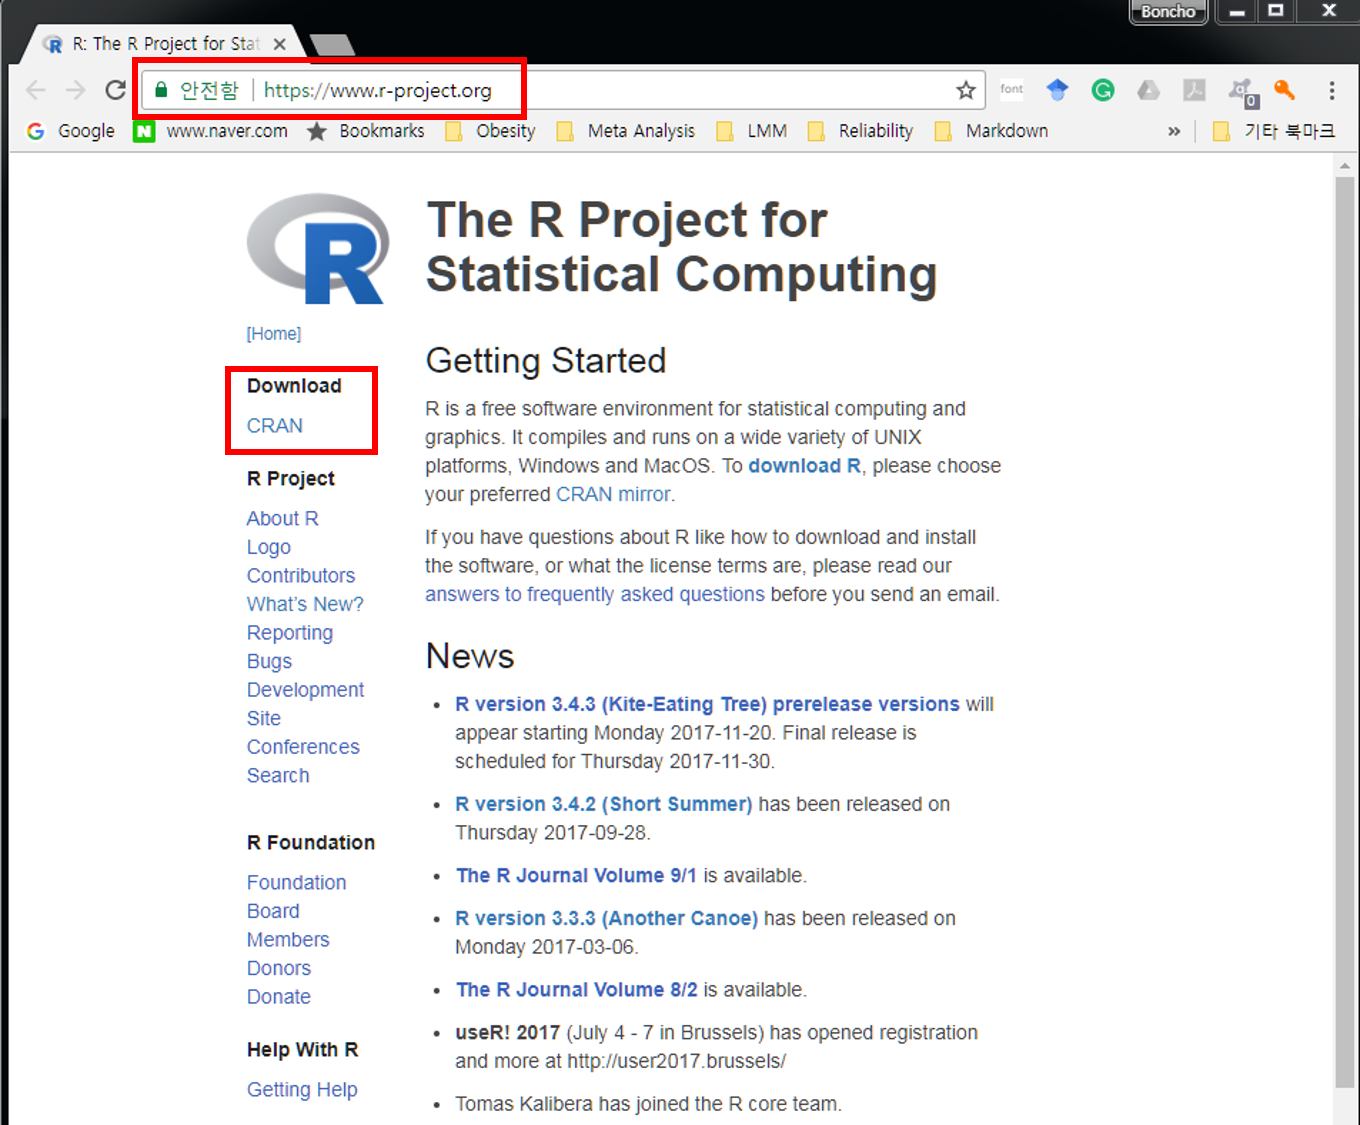
\includegraphics[width=0.9\linewidth]{figures/Rorg-main-add} \end{center}

\normalsize

\begin{enumerate}
\def\labelenumi{\arabic{enumi}.}
\setcounter{enumi}{2}
\tightlist
\item
  클릭 후 연결한 페이지를 스크롤 후 Korea 아래 링크\footnote{해당 링크들은 접속 시점에 따라 변경될 수 있음} 클릭
\end{enumerate}

\footnotesize

\begin{center}
\includegraphics[width=0.9\linewidth]{figures/CRAN-korea-01} \end{center}

\normalsize

\begin{enumerate}
\def\labelenumi{\arabic{enumi}.}
\setcounter{enumi}{3}
\tightlist
\item
  클릭 후 세 가지 운영체제(Linux, Mac OS X, Windowns)에 따른 R 버전 선택 가능\footnote{본 노트는 Windows 버전 설치만 다룸}
\end{enumerate}

\footnotesize

\begin{center}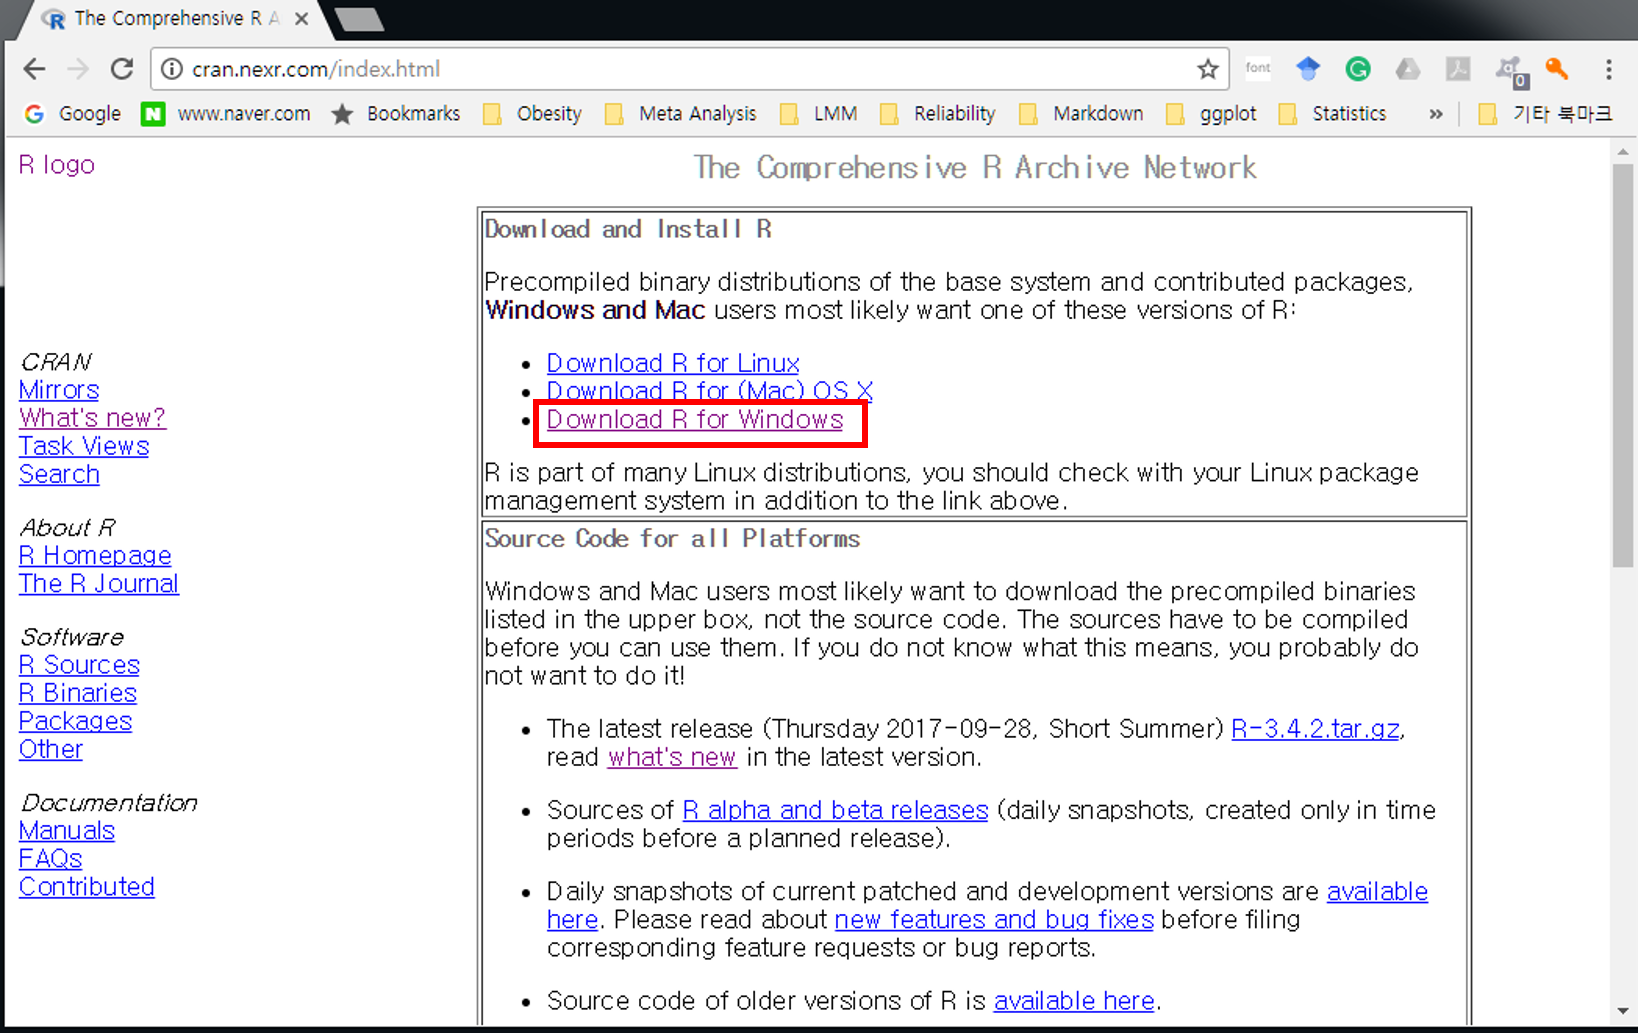
\includegraphics[width=0.9\linewidth]{figures/Rinstall-01} \end{center}

\normalsize

\begin{enumerate}
\def\labelenumi{\arabic{enumi}.}
\setcounter{enumi}{4}
\tightlist
\item
  \textbf{Downloads R for Windows} 링크 클릭하면 다음과 같은 화면으로 이동
\end{enumerate}

\footnotesize

\begin{center}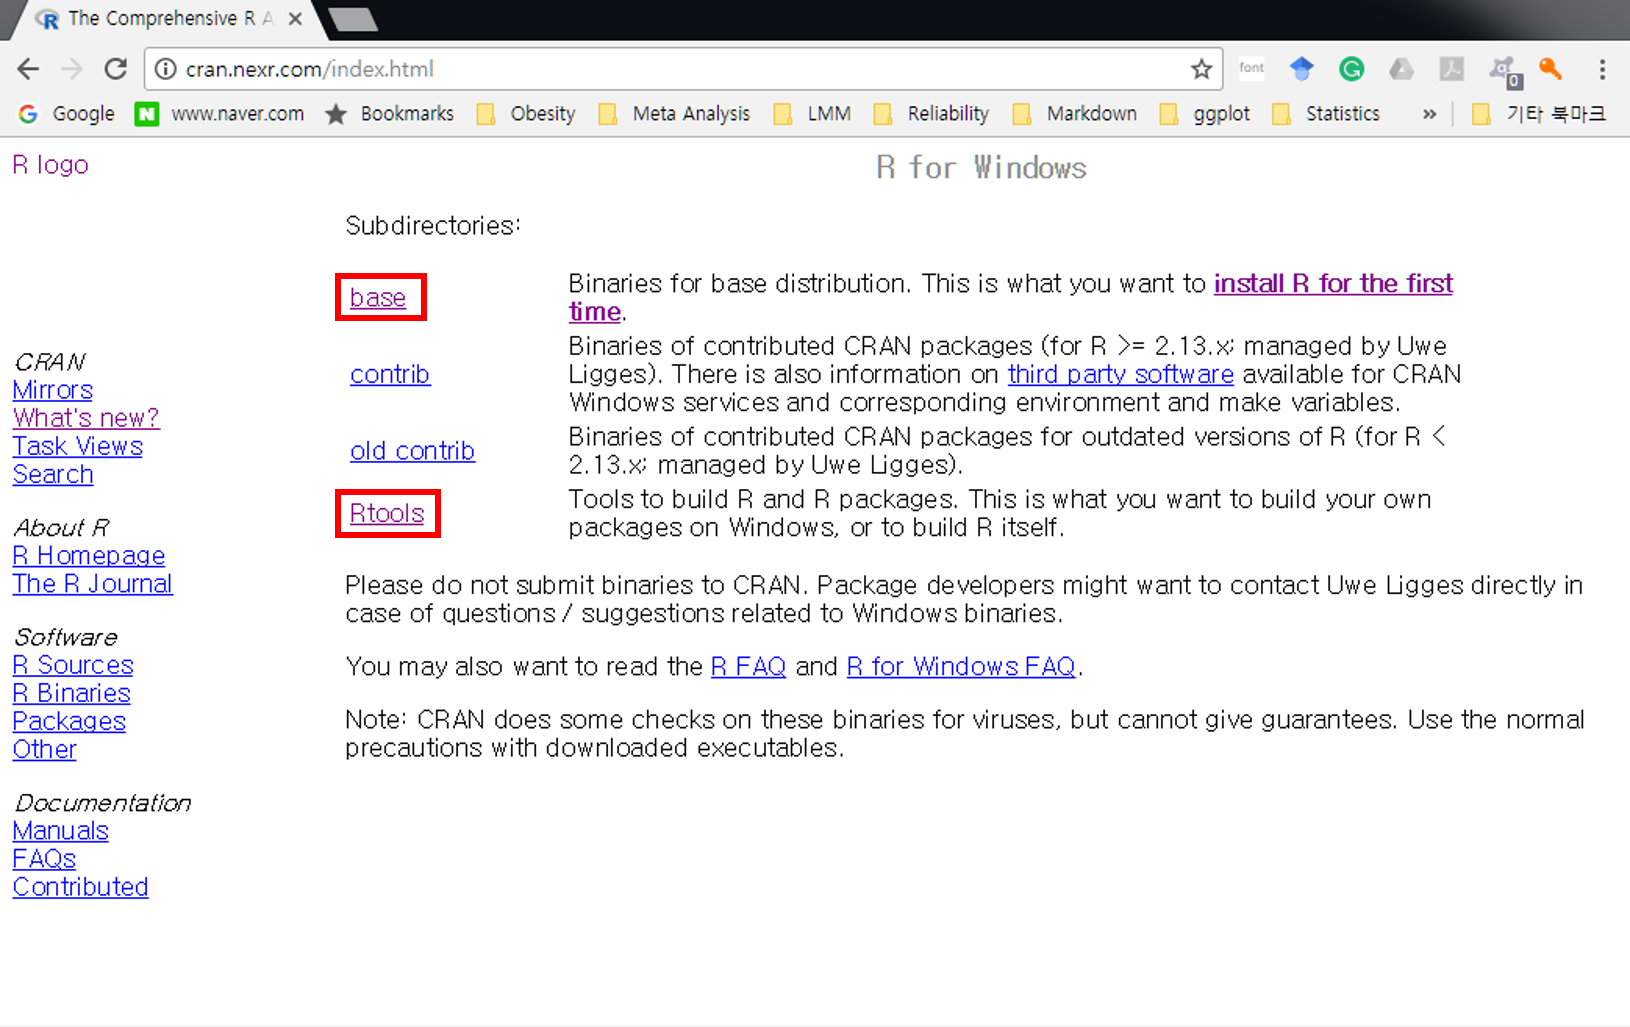
\includegraphics[width=0.9\linewidth]{figures/Rinstall-02} \end{center}

\normalsize

\footnotesize

\begin{rmdtip}
\begin{rmdtip}

다음 하위폴더에 대한 간략 설멍

\begin{itemize}
\tightlist
\item
  \textbf{\texttt{base}}: R 실행 프로그램
\item
  \textbf{\texttt{contrib}}: R package의 바이너리 파일
\item
  \textbf{\texttt{Rtools}}: R package 개발 및 배포를 위한 프로그램
\end{itemize}

\end{rmdtip}
\end{rmdtip}

\normalsize

\begin{enumerate}
\def\labelenumi{\arabic{enumi}.}
\setcounter{enumi}{5}
\tightlist
\item
  위 화면에서 \textbf{base} 링크 클릭 후 아래 화면에서 \textbf{Downloads R 3.x.x for Windows} 를 클릭 후 설치 파일을 임의의 디렉토리에 저장 및 실행
\end{enumerate}

\footnotesize

\begin{center}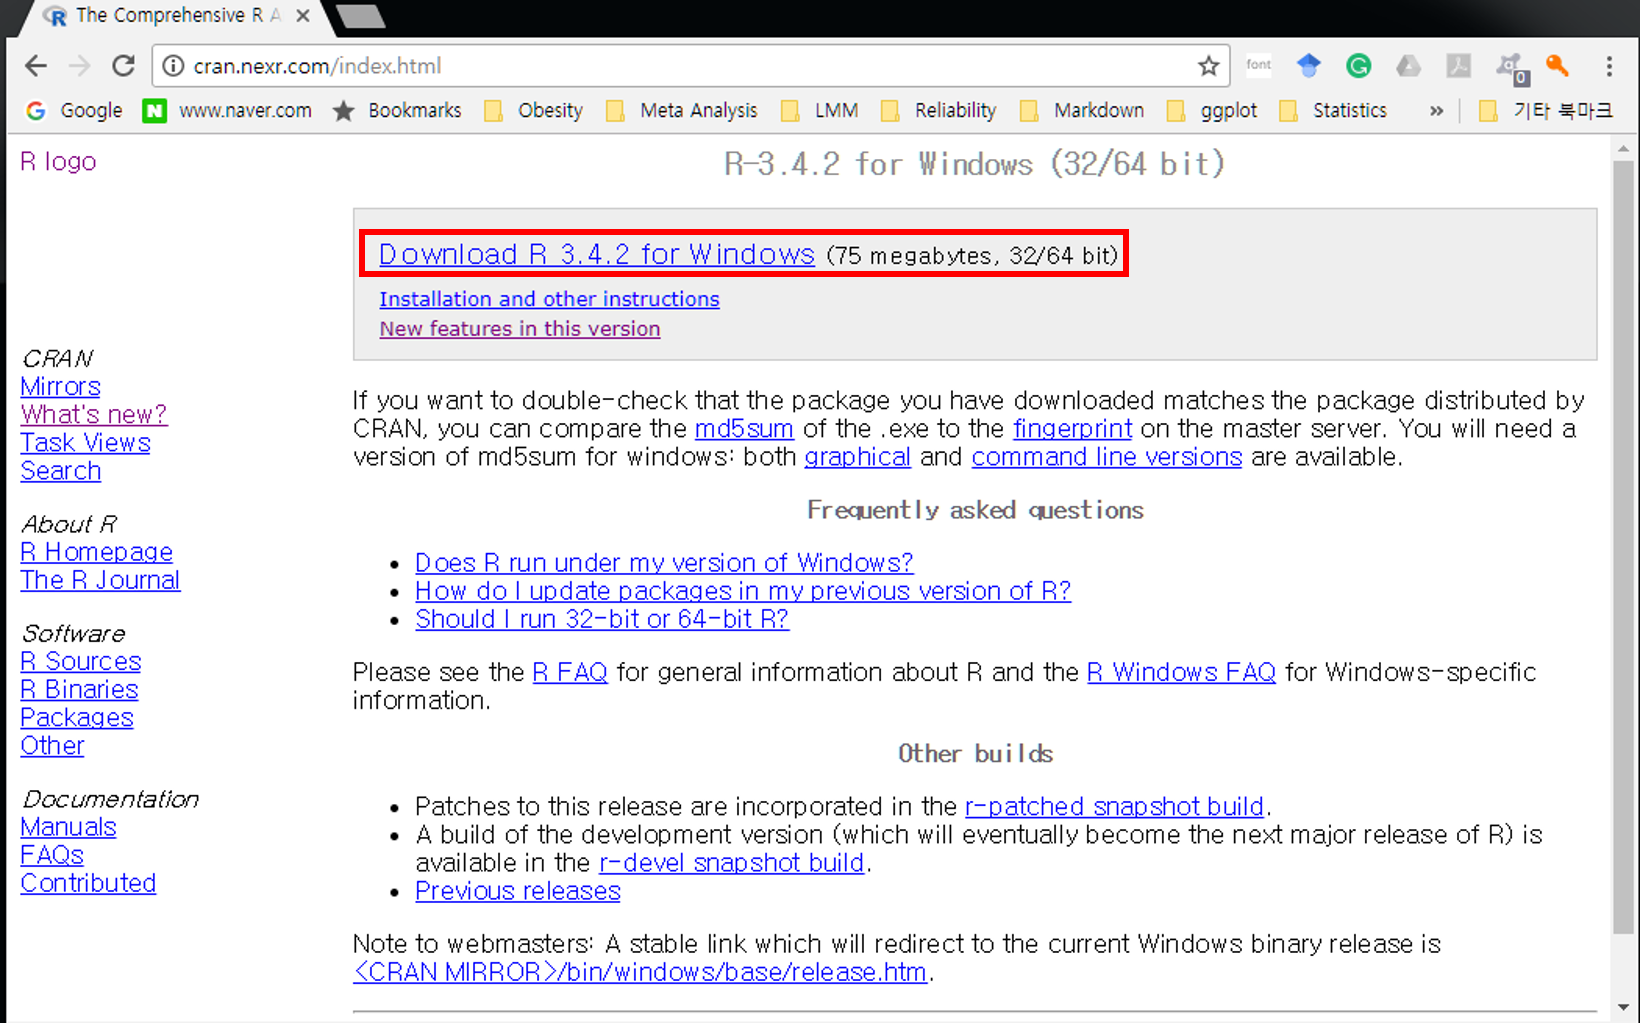
\includegraphics[width=0.9\linewidth]{figures/Rinstall-03} \end{center}

\normalsize

\begin{enumerate}
\def\labelenumi{\arabic{enumi}.}
\setcounter{enumi}{6}
\tightlist
\item
  다운로드한 파일을 실행하면 아래와 같은 대화창이 나타남

  \begin{itemize}
  \tightlist
  \item
    한국어 선택 \(\rightarrow\) 환영 화면에서 {[}다음(N)\textgreater{]} 클릭
  \end{itemize}
\end{enumerate}

\footnotesize

\begin{center}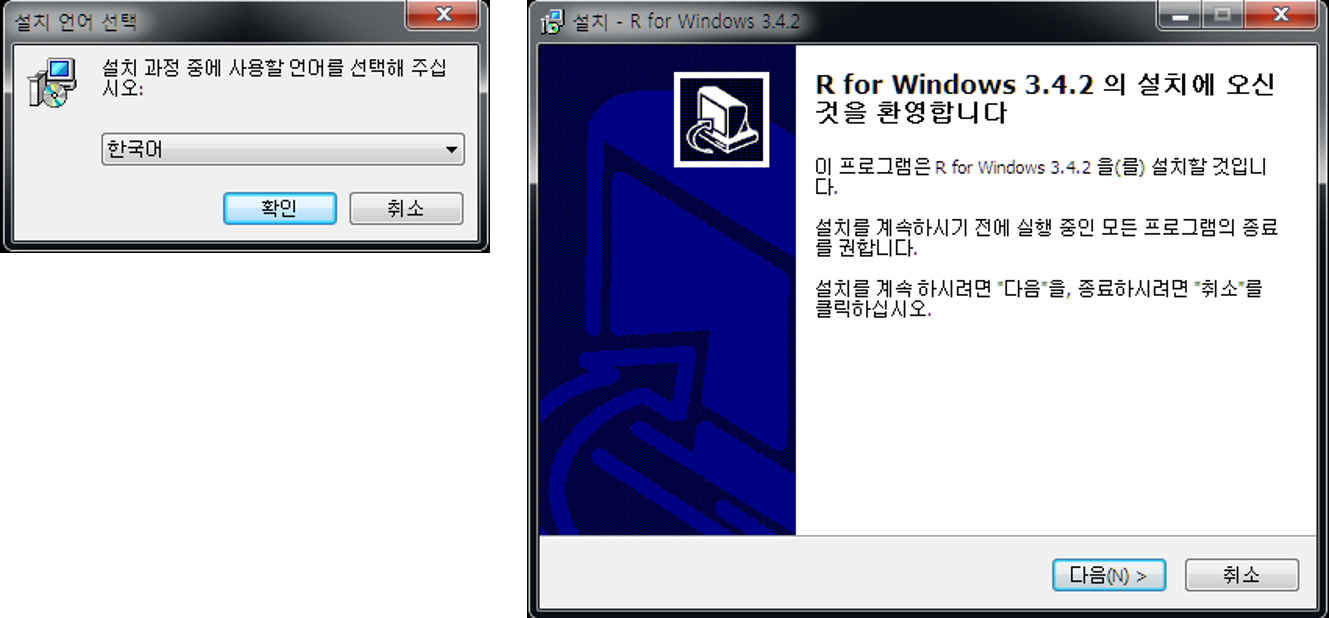
\includegraphics[width=0.9\linewidth]{figures/R-install-F01} \end{center}

\normalsize

\begin{enumerate}
\def\labelenumi{\arabic{enumi}.}
\setcounter{enumi}{7}
\tightlist
\item
  GNU 라이센스에 대한 설명 및 동의 여부({[}다음(N)\textgreater{]}) 클릭
\end{enumerate}

\footnotesize

\begin{center}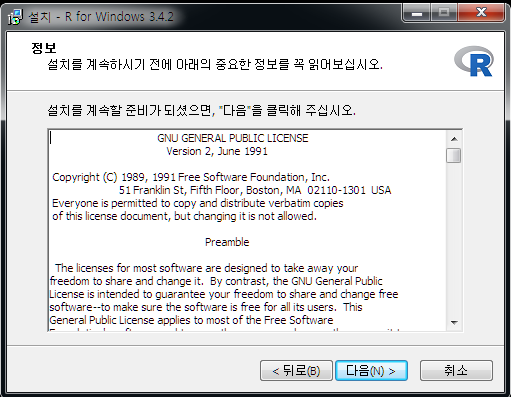
\includegraphics[width=0.9\linewidth]{figures/R-install-F02} \end{center}

\normalsize

\begin{enumerate}
\def\labelenumi{\arabic{enumi}.}
\setcounter{enumi}{8}
\tightlist
\item
  설치 디렉토리 설정 및 구성요소 설지 여부

  \begin{itemize}
  \tightlist
  \item
    원하는 디렉토리 설정(예: \texttt{C:\textbackslash{}R\textbackslash{}R-3.x.x})
  \item
    기본 프로그램(``Core Files''), 32 또는 64 bit 용 설치 파일, R console 한글 번역 모두 체크 뒤 {[}다음(N)\textgreater{]} 클릭
  \end{itemize}
\end{enumerate}

\footnotesize

\begin{center}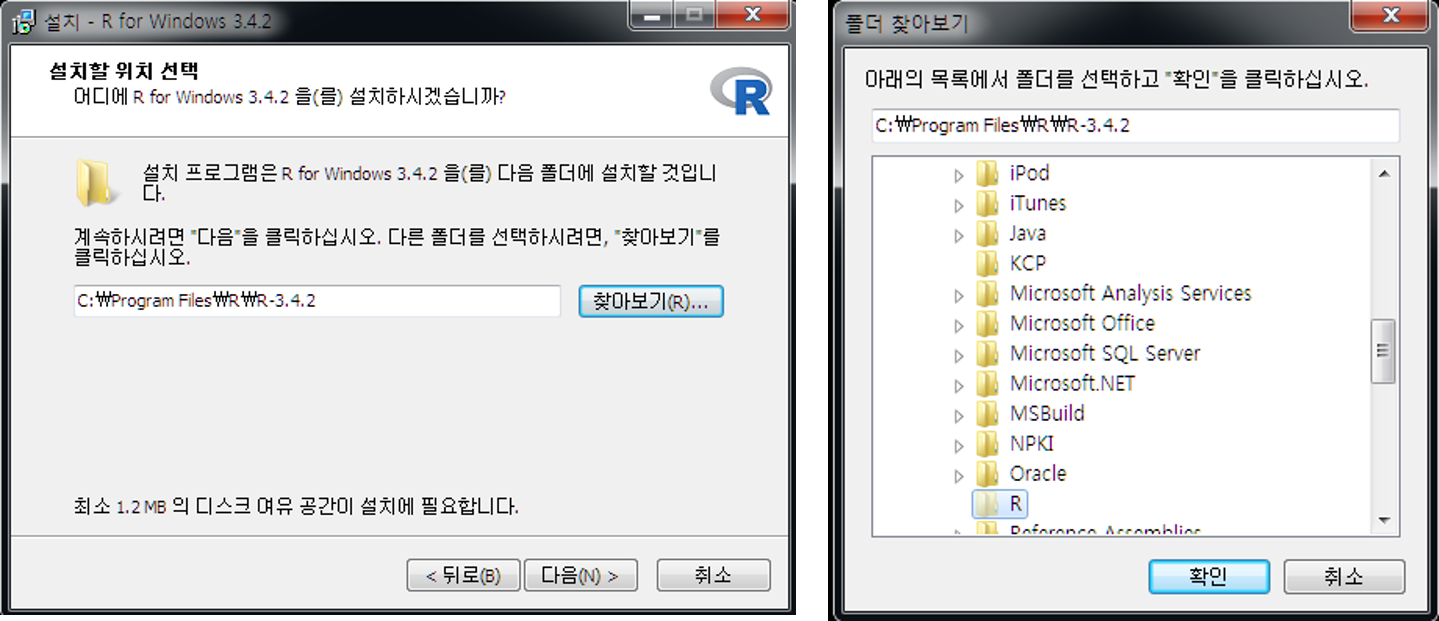
\includegraphics[width=0.9\linewidth]{figures/R-install-F03} \end{center}

\normalsize

\footnotesize

\begin{center}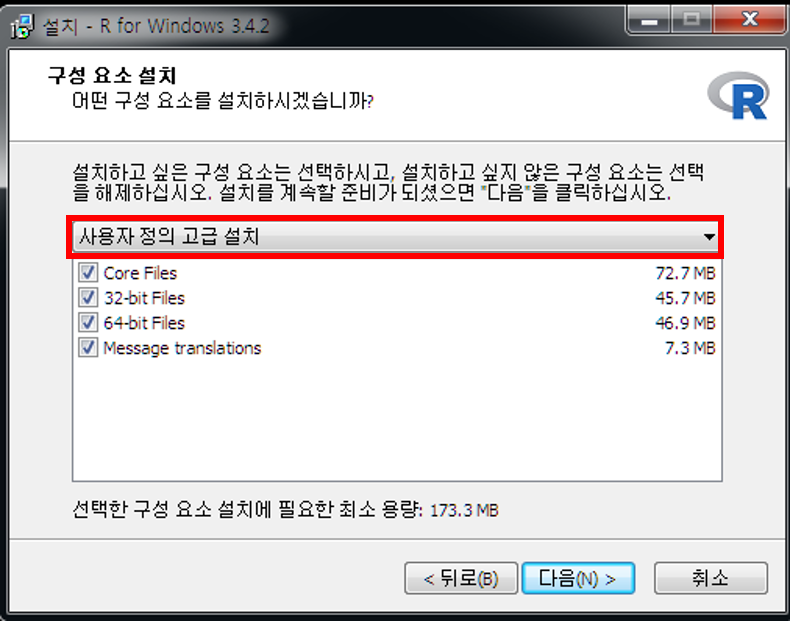
\includegraphics[width=0.9\linewidth]{figures/R-install-F04} \end{center}

\normalsize

\begin{enumerate}
\def\labelenumi{\arabic{enumi}.}
\setcounter{enumi}{9}
\tightlist
\item
  R 스타트업 옵션 지정
\end{enumerate}

\begin{itemize}
\tightlist
\item
  기본값(``No'' check-button)으로도 설치 진행 가능
\item
  본 문서에서는 스타트업 옵션 변경으로 진행
\end{itemize}

\footnotesize

\begin{center}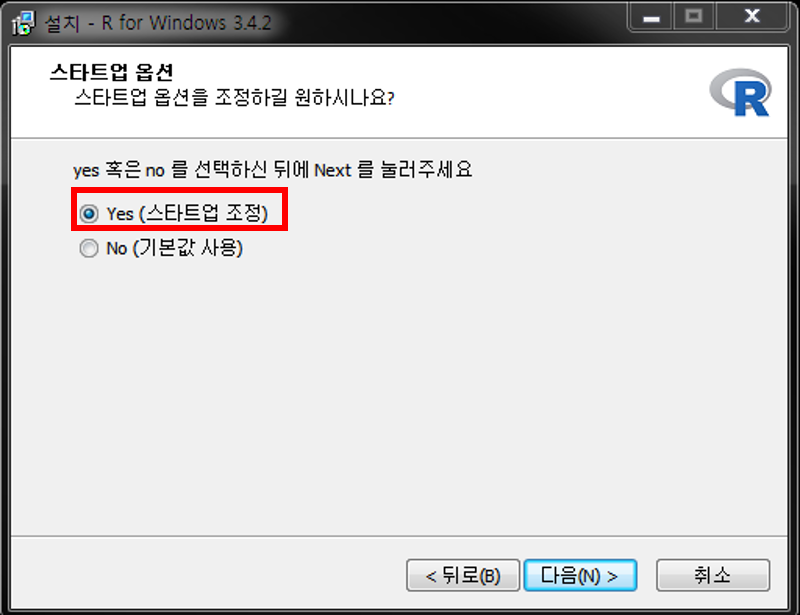
\includegraphics[width=0.9\linewidth]{figures/R-install-F05} \end{center}

\normalsize

\begin{enumerate}
\def\labelenumi{\arabic{enumi}.}
\setcounter{enumi}{10}
\tightlist
\item
  화면표시방식(디스플레이 모드) 설정 변경
\end{enumerate}

\begin{itemize}
\tightlist
\item
  MDI: 한 윈도우 내에서 script 편집창, 출력, 도움말 창 사용
\item
  SDI: 다중 창에서 각각 script 편집창, 출력, 도움말 등을 독립적으로 열기
\end{itemize}

\footnotesize

\begin{center}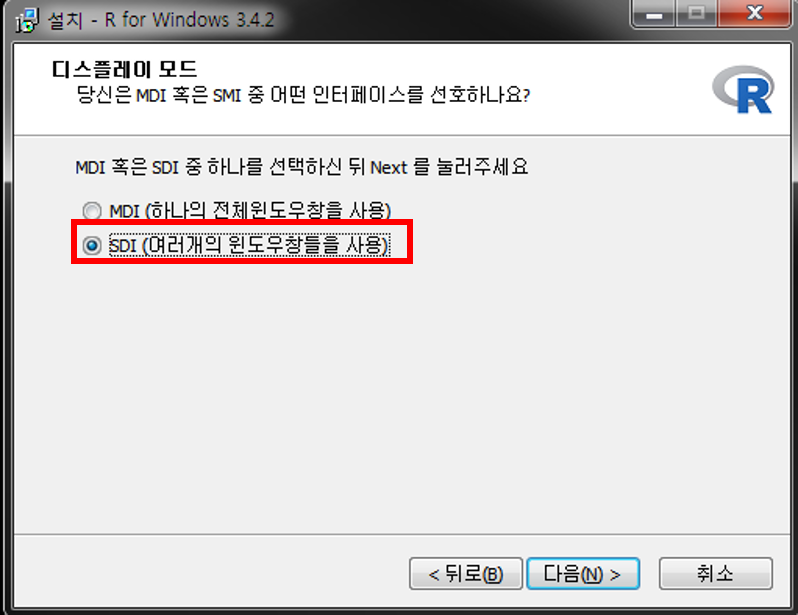
\includegraphics[width=0.9\linewidth]{figures/R-install-F06} \end{center}

\normalsize

\begin{enumerate}
\def\labelenumi{\arabic{enumi}.}
\setcounter{enumi}{11}
\tightlist
\item
  도움말 형식에서 HTML 도움말 기반 선택
\end{enumerate}

\footnotesize

\begin{center}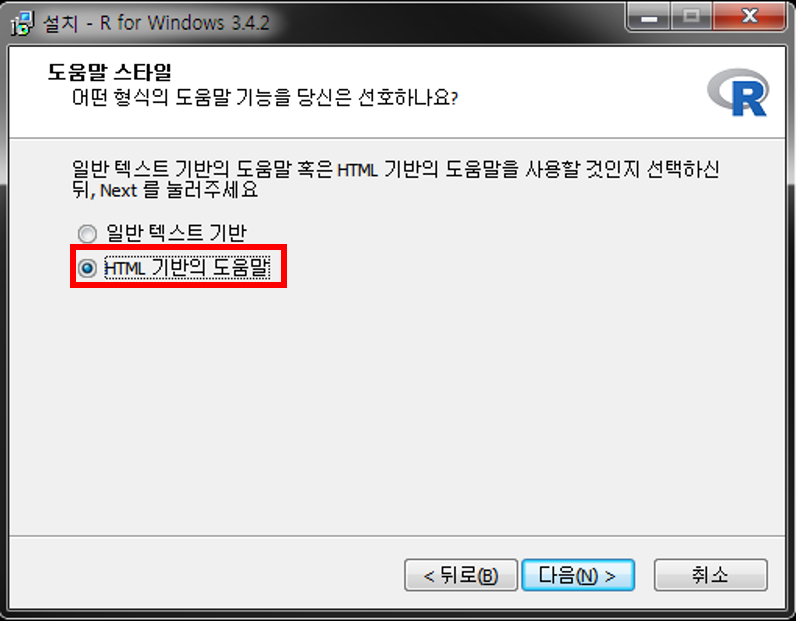
\includegraphics[width=0.9\linewidth]{figures/R-install-F07} \end{center}

\normalsize

\begin{enumerate}
\def\labelenumi{\arabic{enumi}.}
\setcounter{enumi}{12}
\tightlist
\item
  시작메뉴 폴더 선택
\end{enumerate}

\begin{itemize}
\tightlist
\item
  ``바로가기''를 생성할 시작 메뉴 폴더 지정 후 {[}다음(N)\textgreater{]} 클릭 후 설치 진행
\item
  하단 ``시작메뉴 폴더 만들지 않음'' 체크박스 표시 시 시작메뉴에 ``바로가기'' 아이콘이 생성되지 않음(실행에 전혀 지장 없음)
\end{itemize}

\footnotesize

\begin{center}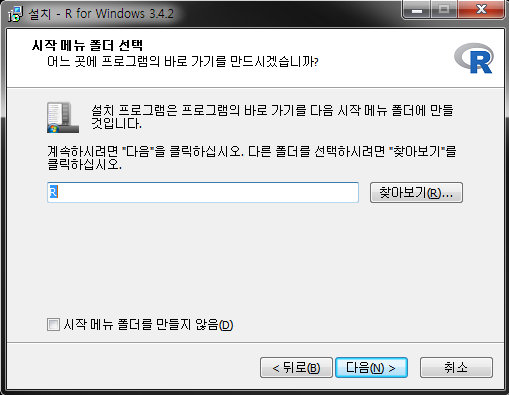
\includegraphics[width=0.9\linewidth]{figures/R-install-F08} \end{center}

\normalsize

\begin{enumerate}
\def\labelenumi{\arabic{enumi}.}
\setcounter{enumi}{13}
\tightlist
\item
  추가 옵션 지정: 바탕화면 아이콘 생성 등 추가적 작업 옵션 체크 후 {[}다음(N)\textgreater{]} 클릭 \(\rightarrow\) 설치 진행
\end{enumerate}

\begin{itemize}
\tightlist
\item
  설치된 R 버전 정보 레지스트리 저장 여부
\item
  \texttt{.Rdata} 확장자를 R 실행파일과 자동 연계
\end{itemize}

\footnotesize

\begin{center}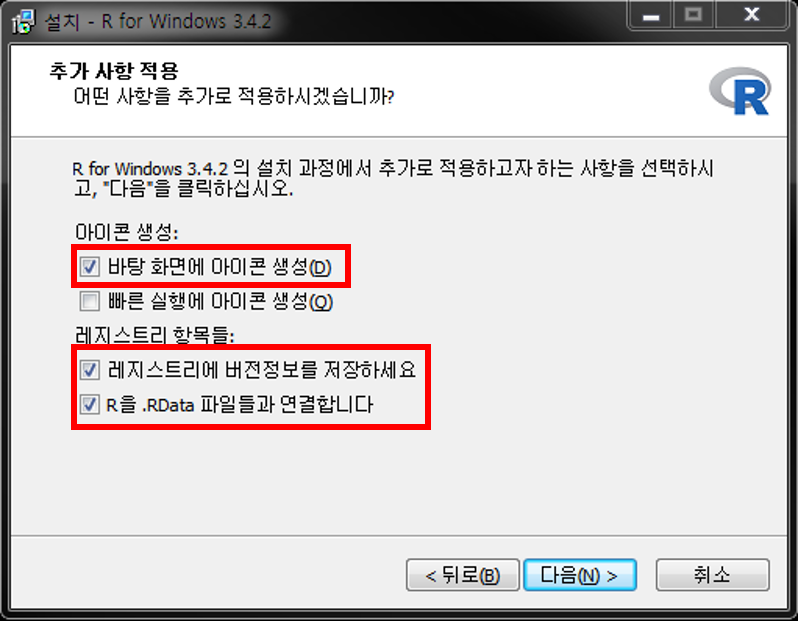
\includegraphics[width=0.9\linewidth]{figures/R-install-F09} \end{center}

\normalsize

\begin{enumerate}
\def\labelenumi{\arabic{enumi}.}
\setcounter{enumi}{14}
\tightlist
\item
  설치 완료 후 바탕화면의 R 아이콘을 더블클릭하면 Rgui가 실행
\end{enumerate}

\footnotesize

\begin{figure}

{\centering 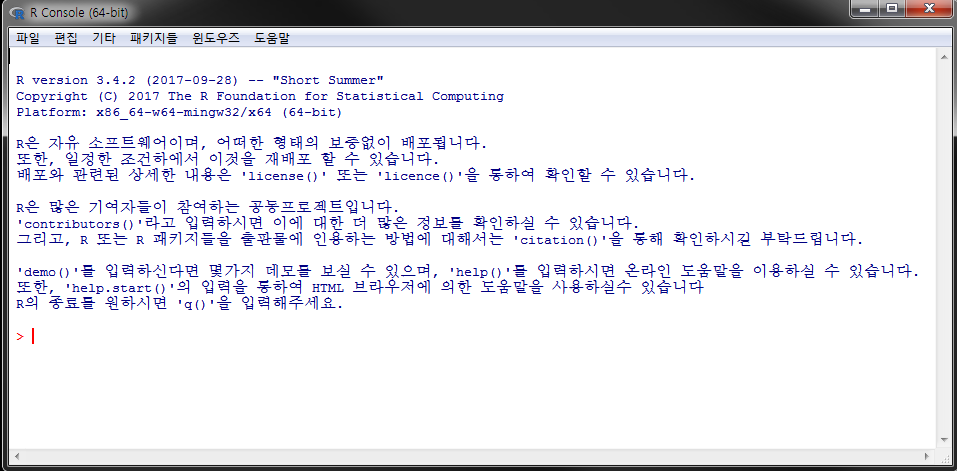
\includegraphics[width=1\linewidth]{figures/Rgui} 

}

\caption{Windows에서 R 실행화면(콘솔 창, SDI 모드)}\label{fig:r-console}
\end{figure}

\normalsize

\hypertarget{r-check}{%
\section{R 시작 및 작동 체크}\label{r-check}}

\begin{rmdimportant}
\begin{rmdimportant}

\textbf{실습}: 설치된 R을 실행 후 보이는 R 콘솔(consle) 창에서 명령어를 실행하고 결과 확인

\end{rmdimportant}
\end{rmdimportant}

Figure \ref{fig:r-console} 에서 \texttt{\textgreater{}} 기호는 R의 명령 프롬프트(command prompt) 임

\begin{itemize}
\tightlist
\item
  \(\rightarrow\) 컴퓨터가 사용자 명령을 기다리고 있다는 기호
\end{itemize}

\begin{enumerate}
\def\labelenumi{\arabic{enumi}.}
\tightlist
\item
  현재 R session\footnote{현재 실행되고 있는 R의 작업공간} 정보(R 설치 버전, locale, 로딩 packages) 출력
\end{enumerate}

\footnotesize

\begin{Shaded}
\begin{Highlighting}[]
\CommentTok{# R의 설치 버전 및 현재 설정된 locale(언어, 시간대) 및 로딩된 R package 정보 출력}
\KeywordTok{sessionInfo}\NormalTok{() }
\end{Highlighting}
\end{Shaded}

\begin{verbatim}
R version 4.0.0 (2020-04-24)
Platform: x86_64-w64-mingw32/x64 (64-bit)
Running under: Windows 10 x64 (build 18363)

Matrix products: default

locale:
[1] LC_COLLATE=Korean_Korea.949  LC_CTYPE=Korean_Korea.949   
[3] LC_MONETARY=Korean_Korea.949 LC_NUMERIC=C                
[5] LC_TIME=Korean_Korea.949    

attached base packages:
[1] stats     graphics  grDevices utils     datasets  methods   base     

other attached packages:
[1] knitr_1.28

loaded via a namespace (and not attached):
 [1] compiler_4.0.0  magrittr_1.5    bookdown_0.19   htmltools_0.4.0
 [5] tools_4.0.0     yaml_2.2.1      Rcpp_1.0.4.6    stringi_1.4.6  
 [9] rmarkdown_2.2   stringr_1.4.0   digest_0.6.25   xfun_0.14      
[13] rlang_0.4.6     evaluate_0.14  
\end{verbatim}

\normalsize

\begin{enumerate}
\def\labelenumi{\arabic{enumi}.}
\setcounter{enumi}{1}
\tightlist
\item
  문자열 출력
\end{enumerate}

\footnotesize

\begin{Shaded}
\begin{Highlighting}[]
\CommentTok{#문자열 출력}
\KeywordTok{print}\NormalTok{(}\StringTok{"Hello R"}\NormalTok{) }\CommentTok{#문자열}
\end{Highlighting}
\end{Shaded}

\begin{verbatim}
[1] "Hello R"
\end{verbatim}

\normalsize

\begin{quote}
\texttt{\#} 기호는 주석의 시작을 의미하고 실제로 실행되지 않음 같은 행에서 \texttt{\#} 뒤 내용의 코드 역시 실행되지 않음
\end{quote}

\begin{enumerate}
\def\labelenumi{\arabic{enumi}.}
\setcounter{enumi}{2}
\tightlist
\item
  \texttt{a} 라는 변수에 숫자 9, \texttt{b}라는 변수에 숫자 7를 할당 후 출력
\end{enumerate}

\footnotesize

\begin{Shaded}
\begin{Highlighting}[]
\CommentTok{# 수치형 값(scalar)을 변수에 할당(assign)}
\CommentTok{# 여러 명령어를 한줄에 입력할 때에는 세미콜론(;)으로 구분}
\NormalTok{a =}\StringTok{ }\DecValTok{9}\NormalTok{; b =}\StringTok{ }\DecValTok{7}
\NormalTok{a}
\end{Highlighting}
\end{Shaded}

\begin{verbatim}
[1] 9
\end{verbatim}

\begin{Shaded}
\begin{Highlighting}[]
\NormalTok{b}
\end{Highlighting}
\end{Shaded}

\begin{verbatim}
[1] 7
\end{verbatim}

\normalsize

\begin{enumerate}
\def\labelenumi{\arabic{enumi}.}
\setcounter{enumi}{3}
\tightlist
\item
  변수 \texttt{a}와 \texttt{b}의 사칙연산
\end{enumerate}

\footnotesize

\begin{Shaded}
\begin{Highlighting}[]
\NormalTok{a}\OperatorTok{+}\NormalTok{b; a}\OperatorTok{-}\NormalTok{b; a}\OperatorTok{*}\NormalTok{b; a}\OperatorTok{/}\NormalTok{b}
\end{Highlighting}
\end{Shaded}

\begin{verbatim}
[1] 16
\end{verbatim}

\begin{verbatim}
[1] 2
\end{verbatim}

\begin{verbatim}
[1] 63
\end{verbatim}

\begin{verbatim}
[1] 1.285714
\end{verbatim}

\normalsize

\begin{enumerate}
\def\labelenumi{\arabic{enumi}.}
\setcounter{enumi}{4}
\tightlist
\item
  R 그래픽 맛보기: 정규분포로부터 난수 100개 생성 후 생성된 데이터에 대한 히스토그램 작성
\end{enumerate}

\footnotesize

\begin{Shaded}
\begin{Highlighting}[]
\CommentTok{# 난수 생성 시 값은 매번 달라지기 때문에 seed를 주어 일정값이 생성되도록 고정}
\CommentTok{# "="과 "<-"는 모두 동일한 기능을 가진 할당 연산자임}
\CommentTok{#평균이 0 이고 분산이 1인 정규분포에서 난수 100개 생성}
\KeywordTok{set.seed}\NormalTok{(}\DecValTok{12345}\NormalTok{) }\CommentTok{# random seed 지정}
\NormalTok{x <-}\StringTok{ }\KeywordTok{rnorm}\NormalTok{(}\DecValTok{100}\NormalTok{) }\CommentTok{# 난수 생성}
\KeywordTok{hist}\NormalTok{(x) }\CommentTok{# 히스토그램}
\end{Highlighting}
\end{Shaded}

\begin{figure}

{\centering 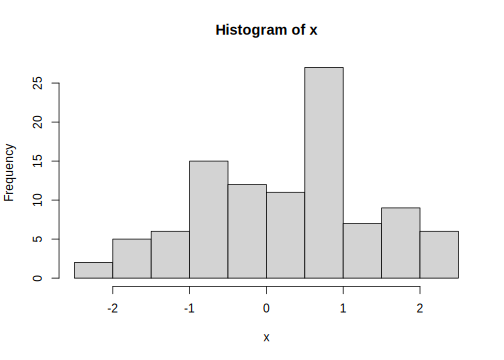
\includegraphics{01-overview_files/figure-latex/check-04-1} 

}

\caption{정규분포 100개의 히스토그램}\label{fig:check-04}
\end{figure}

\normalsize

\footnotesize

\begin{rmdtip}
\begin{rmdtip}

R 명령어 또는 전체 프로그램 소스 실행 시 매우 빈번히 오류가 나타나는데, 이를 해결할 수 있는 가장 좋은 방법은 앞에서 언급한 Google을 이용한 검색 또는 R 설치 시 자체적으로 내장되어 있는 도움말을 참고하는 것이 가장 효율적임.

\end{rmdtip}
\end{rmdtip}

\normalsize

\footnotesize

\begin{table}[H]

\caption{\label{tab:tab-help}R help 관련 명령어 리스트}
\centering
\fontsize{10}{12}\selectfont
\begin{tabular}[t]{l>{\raggedright\arraybackslash}p{5cm}l}
\toprule
도움말 보기 명령어 & 설명 & 사용법\\
\midrule
\rowcolor{gray!6}  `help` 또는 `?` & 도움말 시스템 호출 & `help(함수명)`\\
`help.search` 또는 `??` & 주어진 문자열을 포함한 문서 검색 & `help.search(pattern)`\\
\rowcolor{gray!6}  `example` & topic의 도움말 페이지에 있는 examples section 실행 & `example(함수명)`\\
`vignette` & topic의 pdf 또는 html 레퍼런스 메뉴얼 불러오기 & `vignette(패키지명 또는 패턴)`\\
\bottomrule
\end{tabular}
\end{table}

\normalsize

\footnotesize

\begin{rmdtip}
\begin{rmdtip}

\textbf{Vignette} 의 활용

\begin{itemize}
\tightlist
\item
  \texttt{vignette()}에서 제공하는 문서는 데이터를 기반으로 사용하고자 하는 패키지의 실제 활용 예시를 작성한 문서이기 때문에 초보자들이 R 패키지 활용에 대한 접근성을 높혀줌.
\item
  \texttt{browseVignettes()} 명령어를 통해 vignette을 제공하는 R 패키지 및 해당 vignette 문서 확인 가능
\end{itemize}

\end{rmdtip}
\end{rmdtip}

\normalsize

\hypertarget{rconsle-script}{%
\section{R script 편집기 사용}\label{rconsle-script}}

\begin{rmdimportant}
\begin{rmdimportant}

\textbf{실습}: R 설치 후 Rgui 에서 제공하는 편집기(R editor)에 명령어를 입력하고 실행

\end{rmdimportant}
\end{rmdimportant}

설치된 R을 실행 후 상단 pull-down 메뉴에서 {[}\textbf{File}{]} \(\rightarrow\) {[}\textbf{새 스크립트}{]}를 선택하면 아래 그림과 같이 편집창(R 인스톨 시 SDI 옵션 기준)이 나타남

\footnotesize

\begin{center}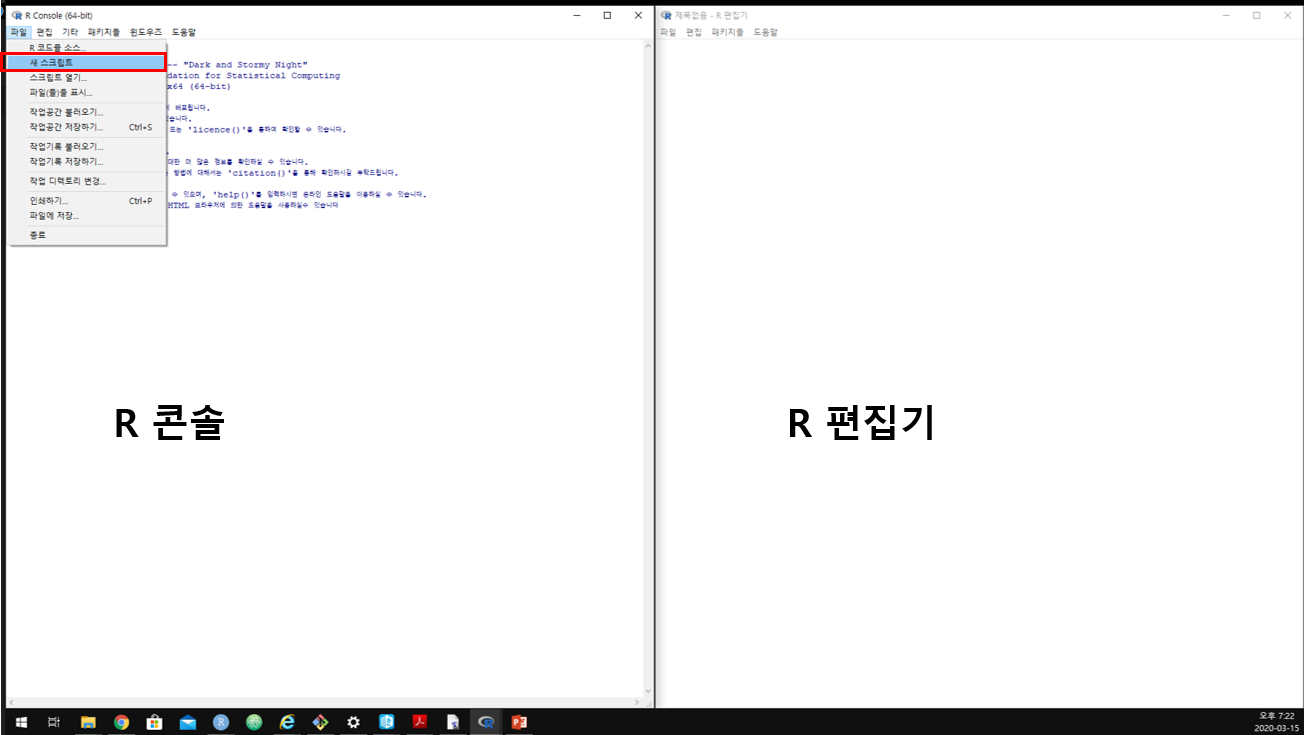
\includegraphics[width=1\linewidth]{figures/r-console-edit} \end{center}

\normalsize

편집기 창에 다음 명령어 입력

\footnotesize

\begin{Shaded}
\begin{Highlighting}[]
\CommentTok{# R에 내장된 cars 데이터셋 불러오기 cars dataset에 포함된 변수들의 기초통계량}
\CommentTok{# 출력 2차원 산점도}
\KeywordTok{data}\NormalTok{(cars)}
\KeywordTok{help}\NormalTok{(cars)  }\CommentTok{# cars 데이터셋에 대한 설명 help 창에 출력}
\KeywordTok{head}\NormalTok{(cars)  }\CommentTok{# cars 데이터셋 처음 6개 행 데이터 출력}
\KeywordTok{summary}\NormalTok{(cars)  }\CommentTok{# cars 데이터셋 요약}
\KeywordTok{plot}\NormalTok{(cars)  }\CommentTok{# 변수가 2개인 경우 산점도 출력}
\end{Highlighting}
\end{Shaded}

\normalsize

\begin{itemize}
\tightlist
\item
  편집창에서 한 줄을 실행시키려면 명령어가 입력된 줄에서 \textbf{{[}Ctrl{]}} + \textbf{{[}R{]}} 입력
\item
  편집창에 입력한 모든 명령어를 실행시키려면 모든 줄을 선택(마우스 또는 {[}Shift{]} + \(\downarrow\))
\end{itemize}

\footnotesize

\begin{verbatim}
  speed dist
1     4    2
2     4   10
3     7    4
4     7   22
5     8   16
6     9   10
\end{verbatim}

\begin{verbatim}
     speed           dist       
 Min.   : 4.0   Min.   :  2.00  
 1st Qu.:12.0   1st Qu.: 26.00  
 Median :15.0   Median : 36.00  
 Mean   :15.4   Mean   : 42.98  
 3rd Qu.:19.0   3rd Qu.: 56.00  
 Max.   :25.0   Max.   :120.00  
\end{verbatim}

\begin{figure}
\centering
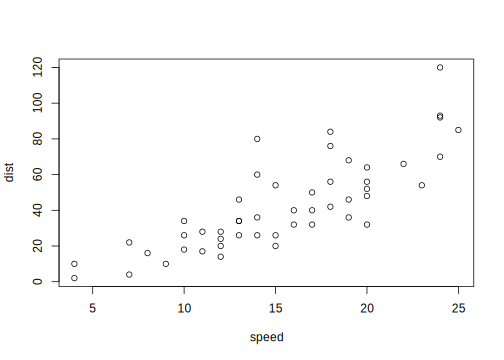
\includegraphics{01-overview_files/figure-latex/check-edit-out-1.pdf}
\caption{\label{fig:check-edit-out}cars 데이터셋의 speed와 dist 간 2차원 산점도: speed는 자동차 속도(mph)이고 dist는 해당 속도에서 브레이크를 밟았을 때 멈출 때 까지 걸린 거리(ft)를 나타냄.}
\end{figure}

\normalsize

\begin{itemize}
\tightlist
\item
  R은 명령어를 입력하고 실행결과를 확인하는 대화형(interpreter) 방식
\item
  콘솔창에서 \(\uparrow\)/\(\downarrow\)를 누르면 이전/이후 실행 명령 기록 확인 가능
\item
  여러 줄 이상 R 명령어라든가 반복적, 장기간 작업을 수행해야 할 경우 R 명령어로 구성된 스크립트 작성 후 일괄 실행하는 것이 일반적
\item
  여러 다중 명령 코딩 시 콘솔창에 직접 입력하는 것은 비효율적이므로 스크립트 에디터를 사용
\item
  위 예시처럼 R 에디터 사용할 수 있으나 가독성 및 코딩 효율이 떨어짐
\item
  과거 많이 사용됐던 R 에디터: \href{http://www.winedt.com}{WinEdt}, \href{https://sourceforge.net/projects/tinn-r/}{Tinn-R}, \href{http://www.vim.org/scripts/script.php?script_id=2628}{Vim}
\item
  현재 가장 범용적 R 에디터: \textbf{Rstudio}
\end{itemize}

\hypertarget{r-studio}{%
\section{RStudio}\label{r-studio}}

\begin{itemize}
\tightlist
\item
  \href{https://rstudio.com/}{RStudio}: R 통합 분석/개발 환경(integrated development environment, IDE)으로 현재 가장 대중적으로 사용되고 있는 R 사용 환경
\item
  명령 곤솔 외 파일 편집, 데이터 객체, 명령 기록(.history), 그래프 등에 쉽게 접근 가능
\item
  RStudio 독자적인 개발 환경 제공: Rmarkdown, Rnotebook, Shiny Web Application 등 다양한 R 환경을 제공
\item
  버전관리(git, subversion)를 통해 project 관리 가능
\item
  \textbf{무료} 및 유료 소프트웨어 제공
\end{itemize}

\hypertarget{rstudio-install}{%
\subsection{RStudio 설치하기}\label{rstudio-install}}

\begin{enumerate}
\def\labelenumi{\arabic{enumi}.}
\tightlist
\item
  웹 브라우저를 통해 \url{https://rstudio.com} 접속 후 상단 \href{https://rstudio.com/products/rstudio/download/}{DOWNLOAD} 링크 클릭
\end{enumerate}

\footnotesize

\begin{center}
\includegraphics[width=0.8\linewidth]{figures/rstudio-homepage} \end{center}

\normalsize

\begin{enumerate}
\def\labelenumi{\arabic{enumi}.}
\setcounter{enumi}{1}
\item
  Desktop 또는 Server 버전 중 택일

  \begin{itemize}
  \tightlist
  \item
    서버용 설치를 위해서는 Server 클릭 \(\rightarrow\) 소규모 자료 분석용으로는 불필요
  \item
    여기서는 \textbf{Desktop} 버전 선택 후 다음 링크로 이동
  \end{itemize}
\end{enumerate}

\footnotesize

\begin{center}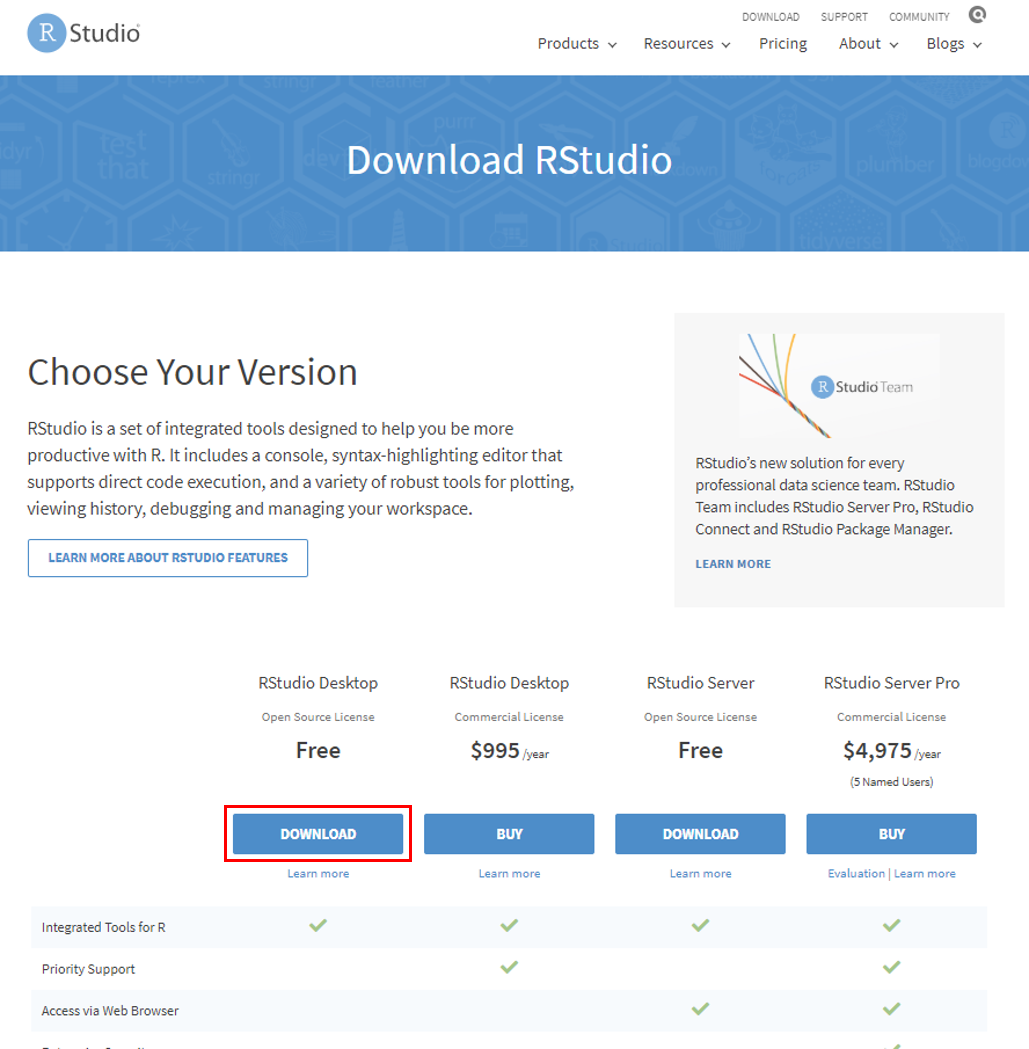
\includegraphics[width=0.7\linewidth]{figures/rstudio-download} \end{center}

\normalsize

\begin{enumerate}
\def\labelenumi{\arabic{enumi}.}
\setcounter{enumi}{2}
\tightlist
\item
  운영체제에 맞는 Rstudio installer 다운로드(여기서는 Windows 버전 다운로드)
\end{enumerate}

\footnotesize

\begin{center}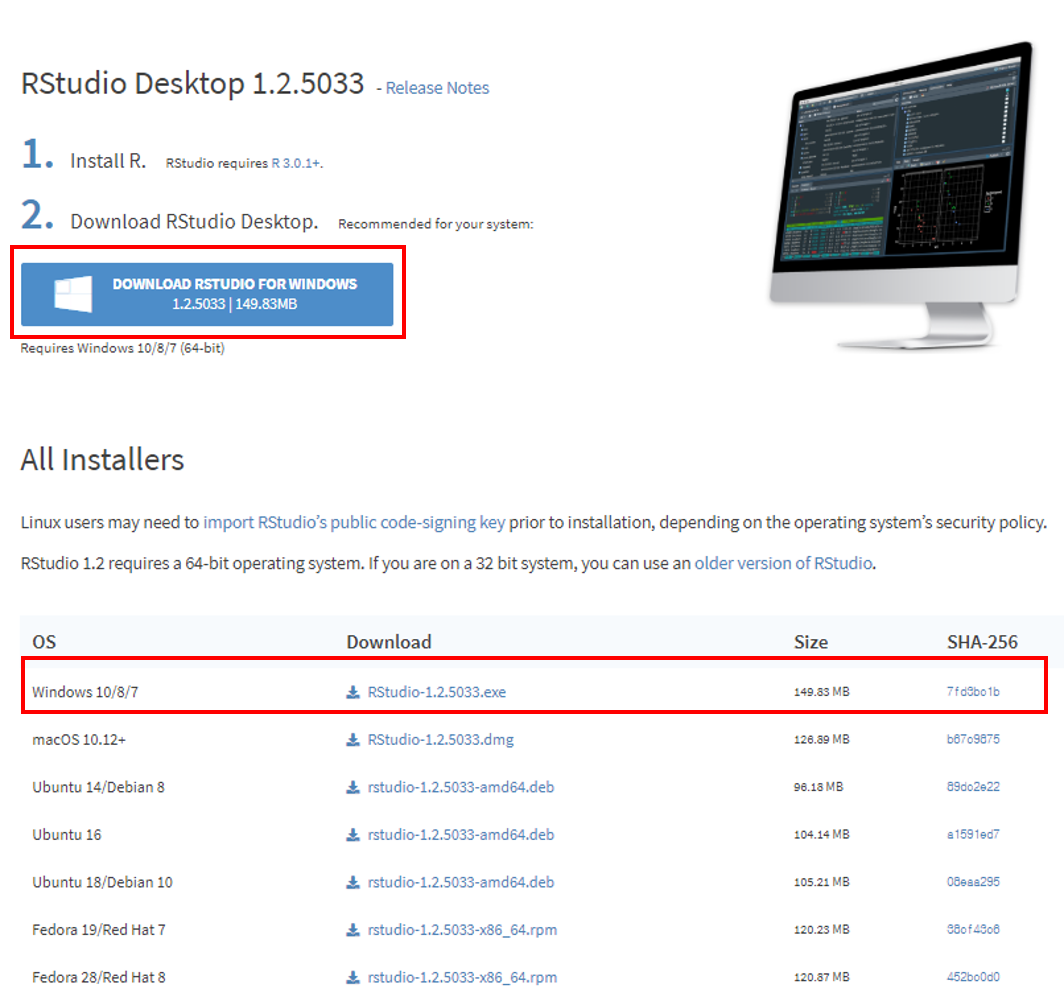
\includegraphics[width=0.6\linewidth]{figures/r-studio-download-02} \end{center}

\normalsize

\begin{enumerate}
\def\labelenumi{\arabic{enumi}.}
\setcounter{enumi}{3}
\tightlist
\item
  RStudio installer 다운로드 시 파일이 저장된 폴더에서 보통 \texttt{RStudio-xx.xx.xxx.exe} 형식의 파일명 확인

  \begin{itemize}
  \tightlist
  \item
    더블 클릭 후 실행
  \item
    \textbf{{[}다음\textgreater{]}} 몇 번 클릭 후 설치 종료
  \end{itemize}
\end{enumerate}

\footnotesize

\begin{center}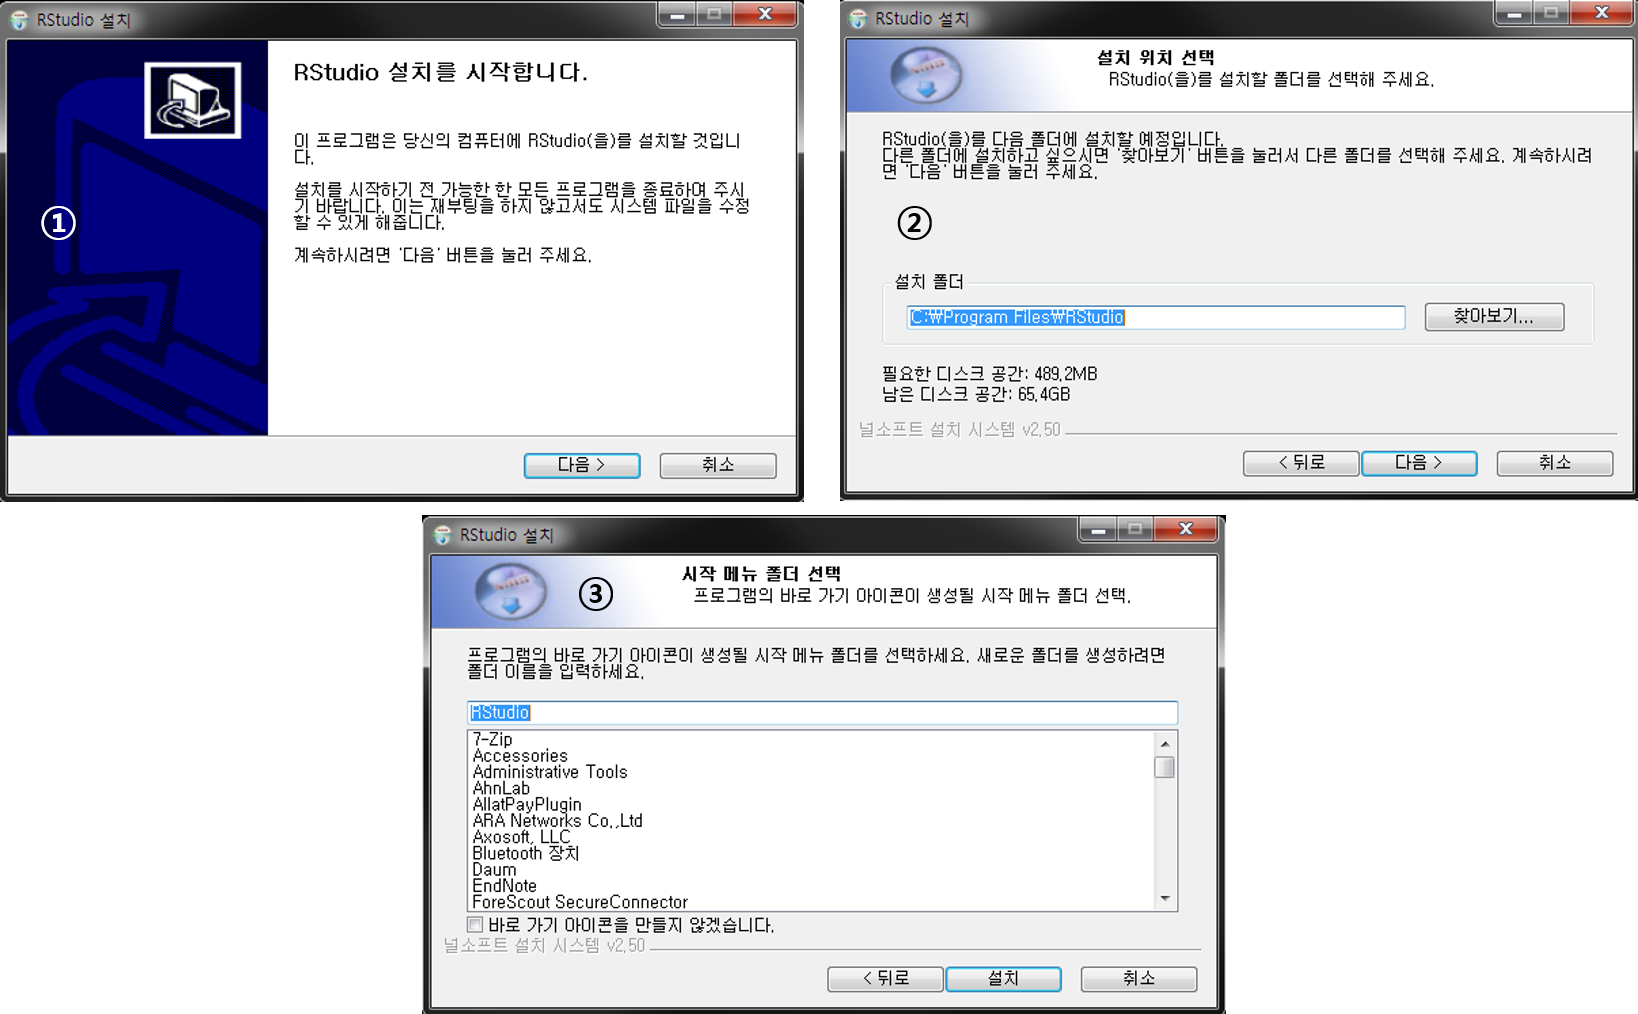
\includegraphics{figures/Rstudio-installer} \end{center}

\normalsize

\begin{enumerate}
\def\labelenumi{\arabic{enumi}.}
\setcounter{enumi}{4}
\tightlist
\item
  바탕화면 혹은 시작 프로그램에 새로 설치된 RStudio 아이콘 클릭 후 아래와 같은 프로그램 창이 나타나면 설치 성공
\end{enumerate}

\footnotesize

\begin{center}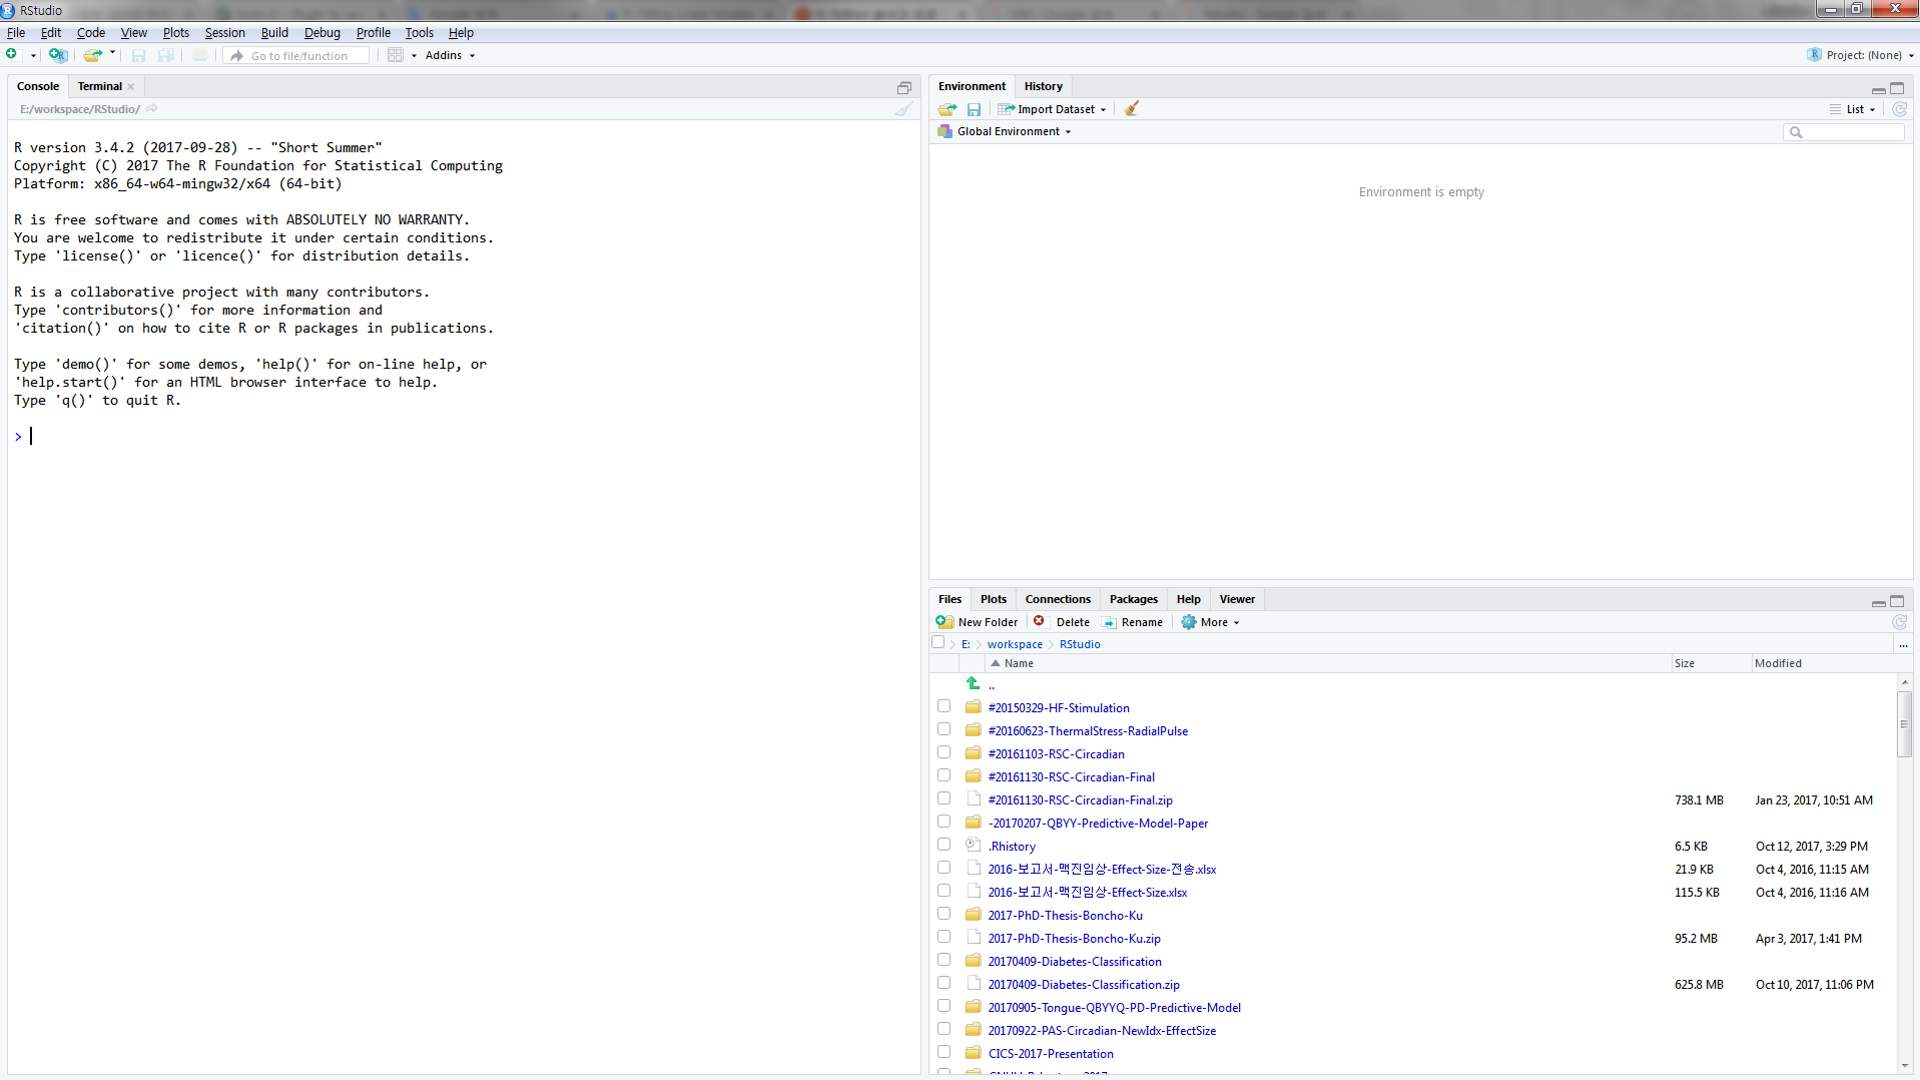
\includegraphics[width=0.8\linewidth]{figures/Rstudio-init} \end{center}

\normalsize

\hypertarget{rstudio-component}{%
\subsection{RStudio IDE 화면 구성}\label{rstudio-component}}

RStudio는 아래 그림과 같이 4개 창으로 구성\footnote{각 창의 위치는 세팅 구성에 따라 달라질 수 있음. 창 구성 방법은 RStudio 환경 옵션 설정에서 설명함.}

\footnotesize

\begin{figure}

{\centering 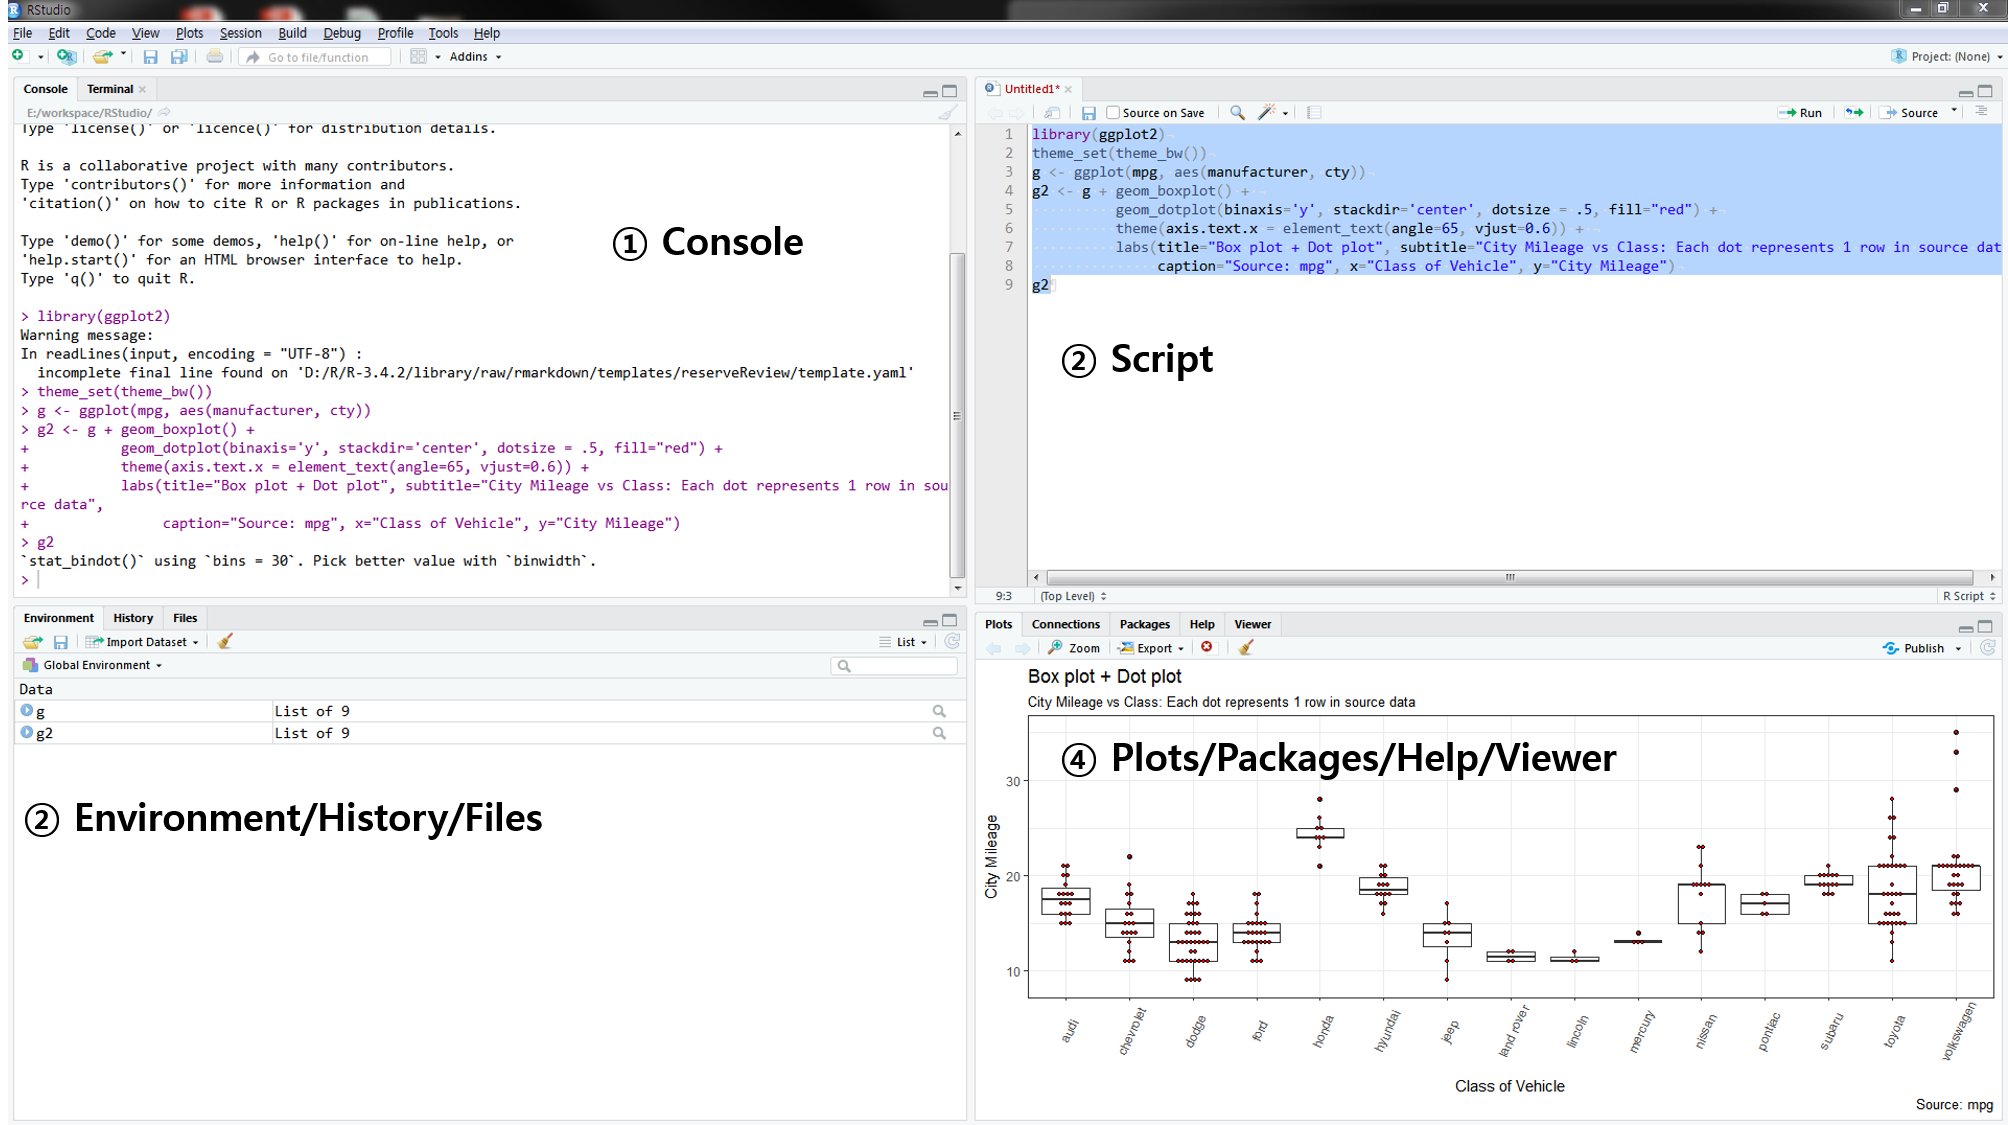
\includegraphics[width=0.9\linewidth]{figures/Rstudio-cap1} 

}

\caption{RStudio 화면구성: 우하단 그림은 http://r-statistics.co/Top50-Ggplot2-Visualizations-MasterList-R-Code.html 에서 발췌}\label{fig:rstudio-windows}
\end{figure}

\normalsize

\textbf{1. 콘솔(console)}

\begin{itemize}
\tightlist
\item
  R 명령어 실행공간(RGui, 정확하게는 R 설치 디렉토리에서 ``\textasciitilde/R/R.x.x/bin/x64/Rterm.exe'' 가 구동되고 있는 공간)
\item
  R script 또는 콘솔 창에서 작성한 명령어(프로그램) 실행 및 그 결과 출력
\item
  경고, 에러/로그 등의 메세지 확인
\end{itemize}

\footnotesize

\begin{figure}

{\centering 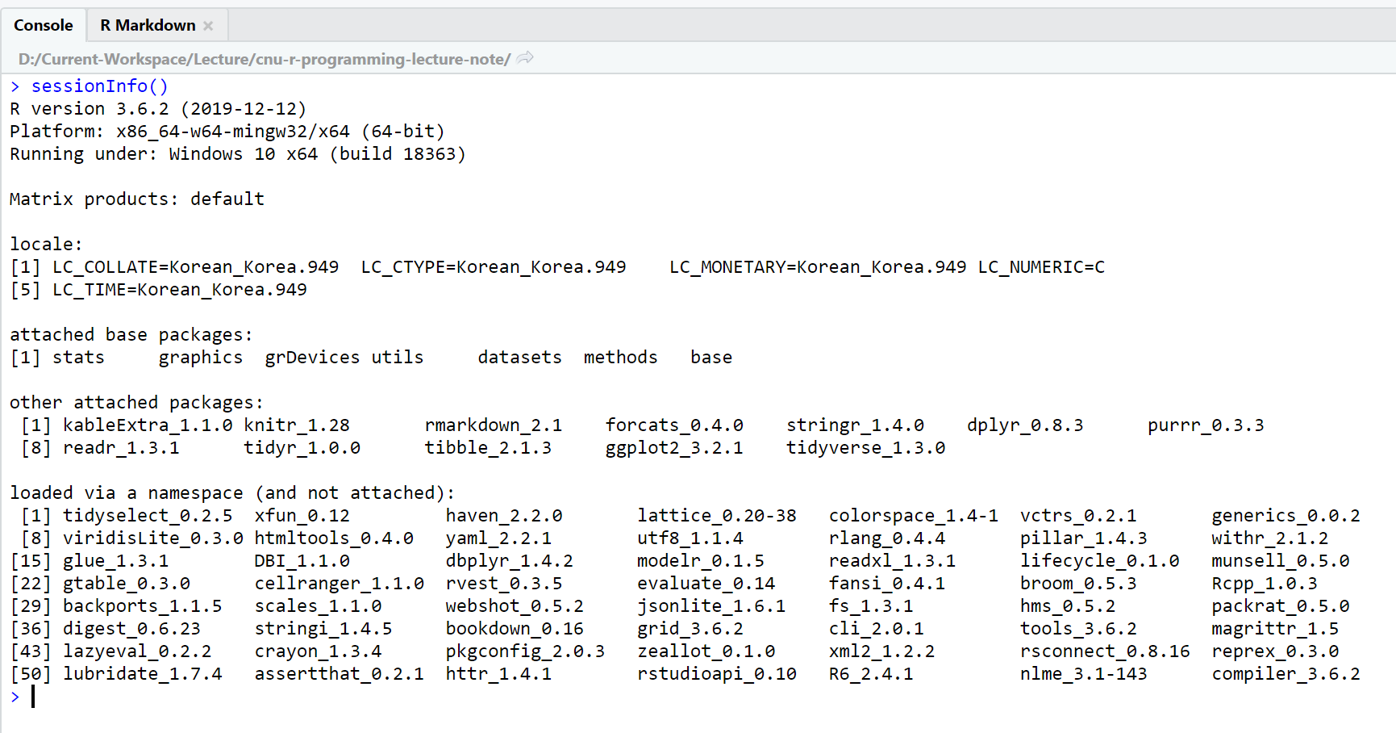
\includegraphics[width=0.8\linewidth]{figures/rstudio-console} 

}

\caption{RStudio 콘솔창에서 명령어 실행 후 출력결과 화면}\label{fig:rstudio-console}
\end{figure}

\normalsize

\textbf{2. 스크립트(script)} (Figure \ref{fig:rstudio-new-script})

\begin{itemize}
\tightlist
\item
  R 명령어 입력 공간으로 일괄처리(batch processing) 가능
\item
  새로운 스크립트 창 열기

  \begin{itemize}
  \tightlist
  \item
    아래 그림과 같이 pull-down 메뉴 좌측 상단 아이콘 클릭 후 {[}R script{]} 선택
  \item
    \texttt{{[}File{]}} \(\rightarrow\) \texttt{{[}New\ File{]}} \(\rightarrow\) \texttt{{[}R\ Script{]}} 선택
  \item
    단축 키: \texttt{{[}Ctrl{]}\ +\ {[}Shift{]}\ +\ {[}N{]}}
  \end{itemize}
\item
  일괄 명령어 처리를 위한 RStudio 제공 단축 키

  \begin{itemize}
  \tightlist
  \item
    \texttt{{[}Ctrl{]}\ +\ {[}Enter{]}}: 선택한 블럭 내 명령어 실행
  \item
    \texttt{{[}Alt{]}\ +\ {[}Enter{]}}: 선택 없이 커서가 위치한 라인의 명령어 실행
  \end{itemize}
\item
  R 스크립트 이외 R Markdown, R Notebook, Shiny web application 등 새 문서의 목적에 따라 다양한 종류의 소스 파일 생성 가능
\item
  저장된 R 스크립트 파일은 \texttt{파일명.R}로 저장됨
\item
  파일 실행 방법

  \begin{itemize}
  \tightlist
  \item
    실행하고자 하는 파일을 읽은 후(\texttt{{[}File{]}} \(\rightarrow\) \texttt{{[}Open\ File{]}} + 파일명 선택 또는 \texttt{파일명.R} 더블 클릭) 입력된 모든 라인을 선택한 뒤 \texttt{{[}Ctrl{]}\ +\ {[}Enter{]}}
  \item
    파일 읽은 후 \texttt{{[}Ctrl{]}\ +\ {[}Shift{]}\ +\ {[}S{]}} (현재 열려있는 \texttt{*.R} 파일에 대해) 또는 \texttt{{[}Ctrl{]}\ +\ {[}Shift{]}\ +\ {[}Enter{]}}
  \end{itemize}
\end{itemize}

\footnotesize

\begin{figure}

{\centering 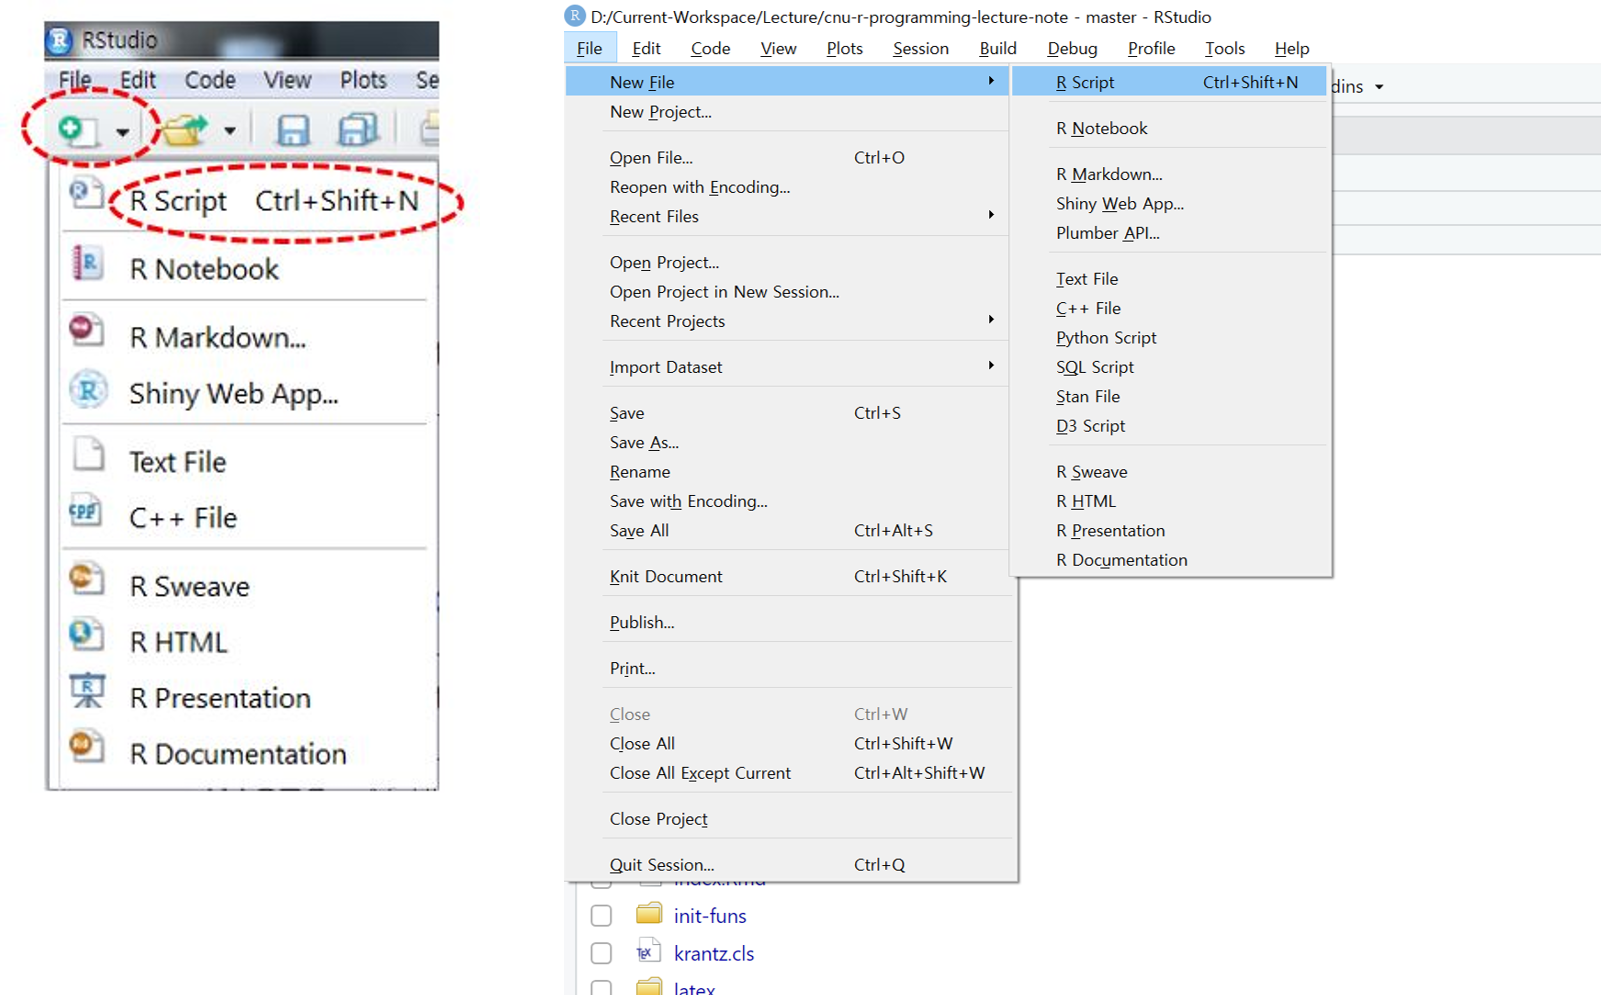
\includegraphics[width=0.8\linewidth]{figures/rstudio-open-new-script} 

}

\caption{RStudio 스크립트 새로 열기}\label{fig:rstudio-new-script}
\end{figure}

\normalsize

\footnotesize

\begin{rmdtip}
\begin{rmdtip}

RStudio는 코딩 및 소스 작성의 효율성을 위해 여러 가지 단축 키를 제공하고 있음. 단축키는 아래 그림과 같이 pull down 메뉴 \texttt{{[}Tools{]}} 또는 \texttt{{[}Help{]}}에서 \texttt{{[}Keyboard\ shortcut\ help{]}} 또는 \texttt{{[}Alt{]}\ +\ {[}Shift{]}\ +\ {[}K{]}} 단축키를 통해 확인할 수 있음. 또는 Rstudio cheatsheet에서 단축키에 대한 정보를 제공하는데 pull down 메뉴 \texttt{{[}Help{]}} \(\rightarrow\) \texttt{{[}Cheatsheets{]}} \(\rightarrow\) \texttt{{[}RStudio\ IDE\ Cheat\ Sheet{]}}을 선택하면 각 아이콘 및 메뉴 기능에 대한 개괄적 설명 확인 가능함.

\end{rmdtip}
\end{rmdtip}

\normalsize

\textbf{3. 환경/명령기록(Environment/History)} (Figure \ref{fig:rstudio-env})

\begin{itemize}
\tightlist
\item
  \textbf{Environment}: 현재 R 작업환경에 저장되어 있는 객체의 특성 및 값 등을 요약 제시

  \begin{itemize}
  \tightlist
  \item
    좌측 아래 화살표 버튼 클릭: 해당 객체의 상세 정보 확인
  \item
    우측 사각형 버튼 또는 객체(데이터셋명) 클릭: 객체가 데이터셋(데이터프레임)인 경우 스프레드 시트 형태로 데이터셋 확인
  \end{itemize}
\end{itemize}

\footnotesize

\begin{figure}

{\centering 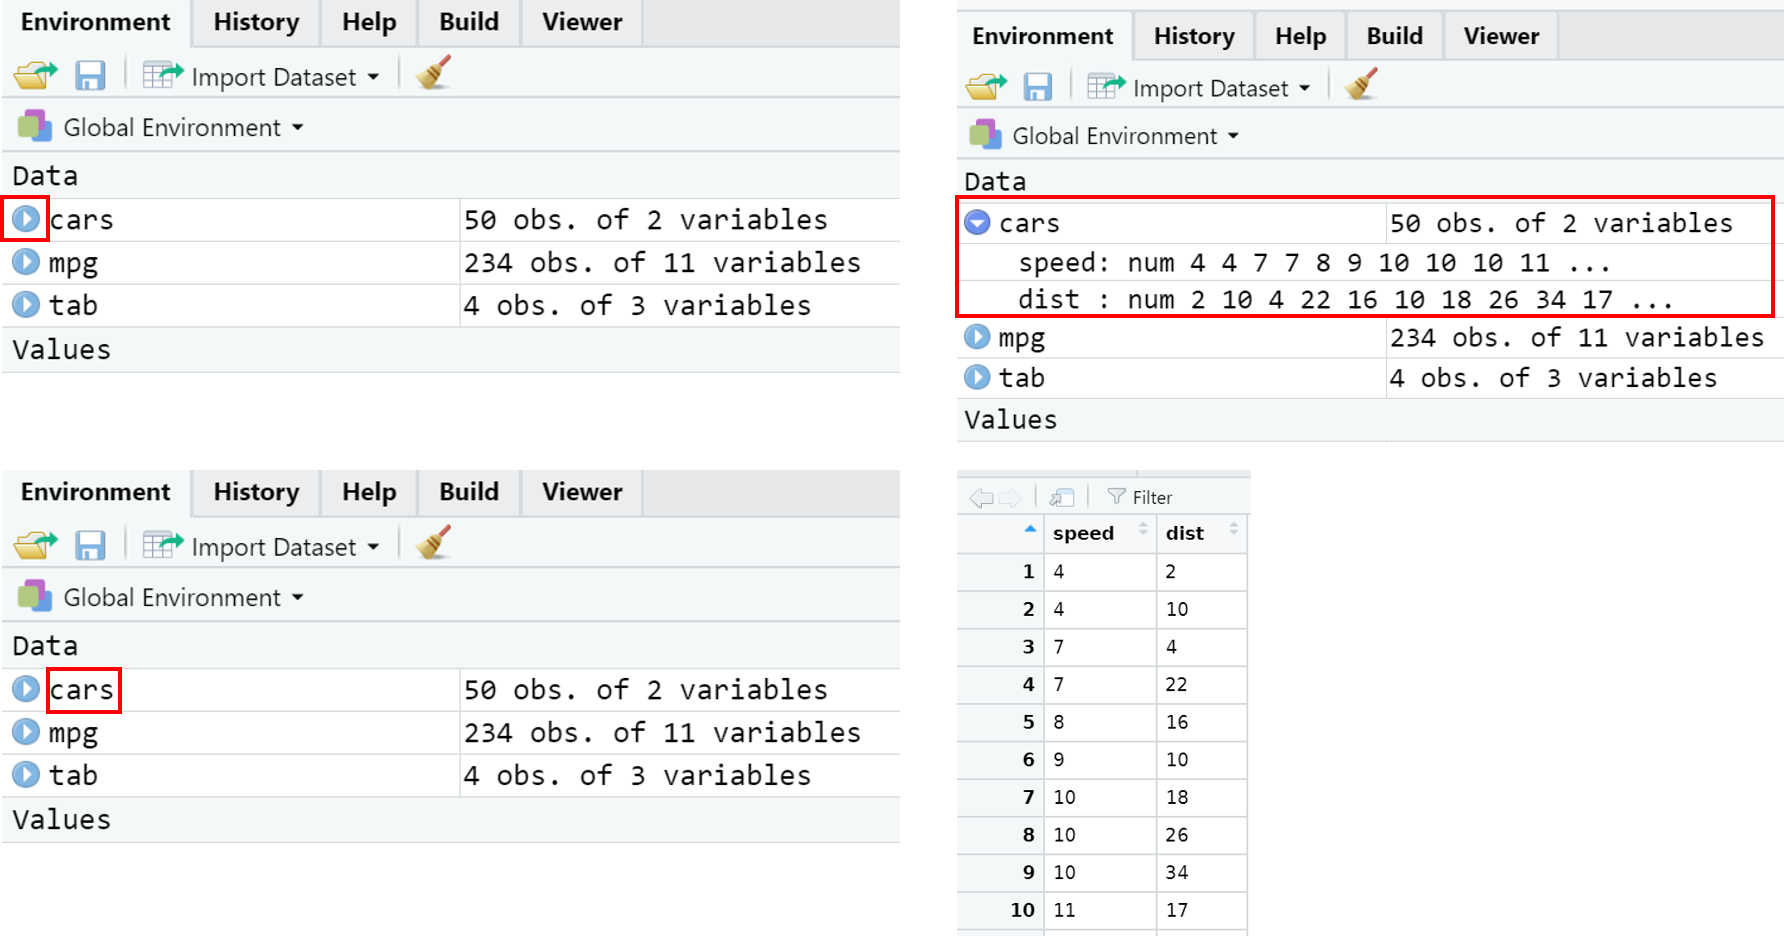
\includegraphics[width=0.9\linewidth]{figures/rstudio-environment} 

}

\caption{RStudio Environment 창 객체 상세 정보 및 스프레드 시트 출력 결과}\label{fig:rstudio-env}
\end{figure}

\normalsize

\begin{itemize}
\tightlist
\item
  History: R 콘솔에서 실행된 명령어(스크립트)들의 이력 확인
\end{itemize}

\footnotesize

\begin{center}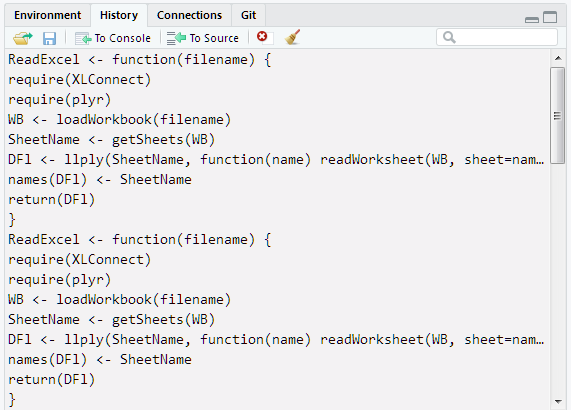
\includegraphics[width=0.9\linewidth]{figures/Rstudio-historywin} \end{center}

\normalsize

\textbf{4. File/Plots/Packages/Help/Viewer}

\begin{itemize}
\tightlist
\item
  File: Windows 파일 탐색기와 유사한 기능 제공

  \begin{itemize}
  \tightlist
  \item
    파일 및 폴더 생성, 삭제/파일 및 폴더명 수정, 그리고 작업경로 설정
  \end{itemize}
\end{itemize}

\footnotesize

\begin{center}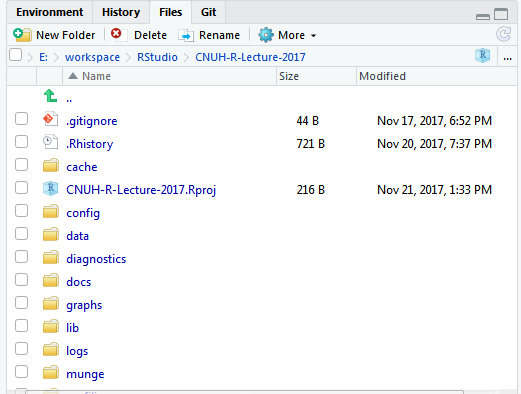
\includegraphics[width=0.8\linewidth]{figures/Rstudio-file} \end{center}

\normalsize

\begin{itemize}
\tightlist
\item
  \textbf{Plots}: 생성한 그래프 출력

  \begin{itemize}
  \tightlist
  \item
    작업 중 생성한 그래프 이력이 Plots 창에 저장: \(\leftarrow\) 이전, \(\rightarrow\) 최근
  \item
    \textbf{\texttt{Zoom}}: 클릭 시 해당 그래프의 팝업창이 생성되고 팝업창의 크기 조정을 통해 그래프의 축소/확대 가능
  \item
    \textbf{\texttt{Export}}: 선택한 그래프를 이미지 파일(\texttt{.png}, \texttt{.jpeg}, \texttt{.pdf} 등)로 저장할 수 있고, 클립보드로 복사 가능
  \end{itemize}
\end{itemize}

\footnotesize

\begin{center}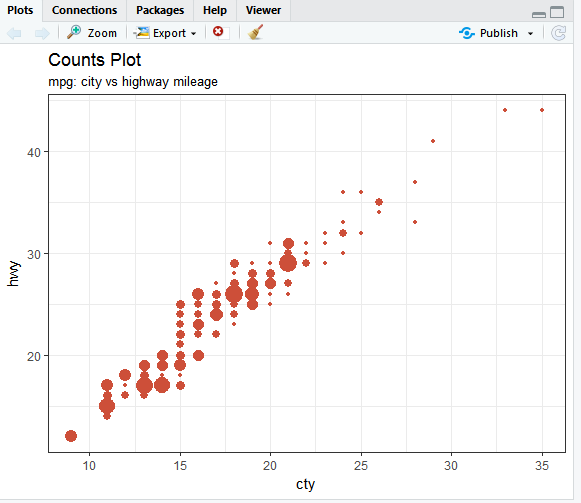
\includegraphics[width=0.8\linewidth]{figures/RStudio-plotwin} \end{center}

\normalsize

\begin{itemize}
\tightlist
\item
  \textbf{Packages}: 현재 컴퓨터에 설치된 R 패키지 목록 출력

  \begin{itemize}
  \tightlist
  \item
    신규 설치 및 업데이트 가능
  \end{itemize}
\end{itemize}

\footnotesize

\begin{center}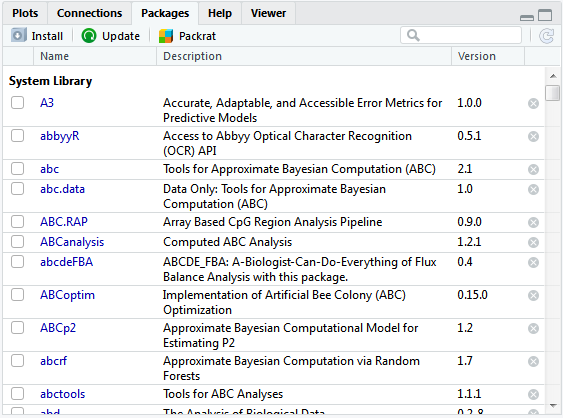
\includegraphics[width=0.8\linewidth]{figures/RStudio-packagewin} \end{center}

\normalsize

\begin{itemize}
\tightlist
\item
  \textbf{Help}: \texttt{help(topic)} 입력 시 도움말 창이 출력되는 공간
\end{itemize}

\footnotesize

\begin{Shaded}
\begin{Highlighting}[]
\KeywordTok{help}\NormalTok{(lm)}
\end{Highlighting}
\end{Shaded}

\normalsize

\footnotesize

\begin{center}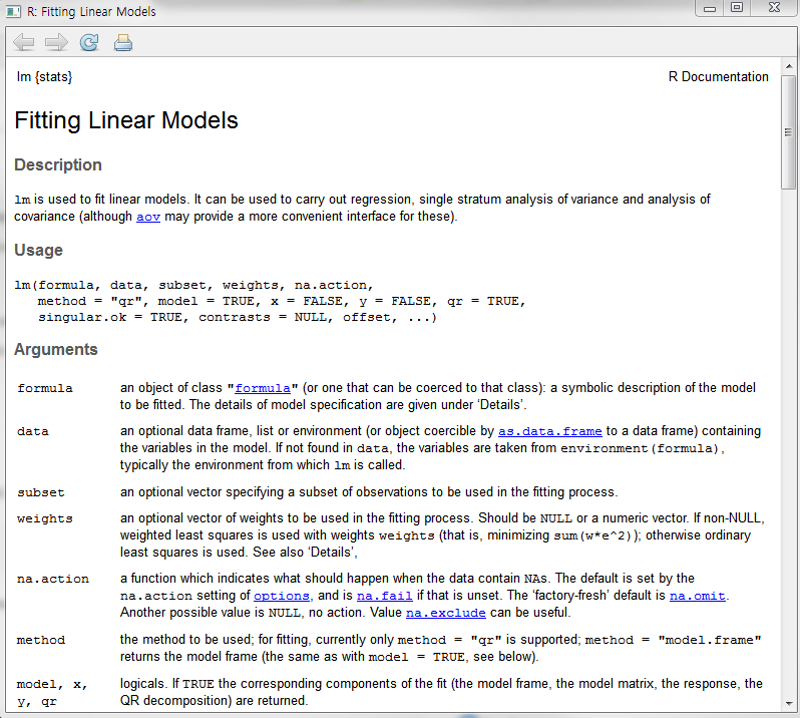
\includegraphics[width=0.8\linewidth]{figures/RStudio-helpwin} \end{center}

\normalsize

\hypertarget{rstudio-glob-options}{%
\subsection{RStudio 환경 설정}\label{rstudio-glob-options}}

Pull-down 메뉴에서 \texttt{{[}Tools{]}} \(\rightarrow\) \texttt{{[}Global\ Options...{]}}를 선택

\footnotesize

\begin{center}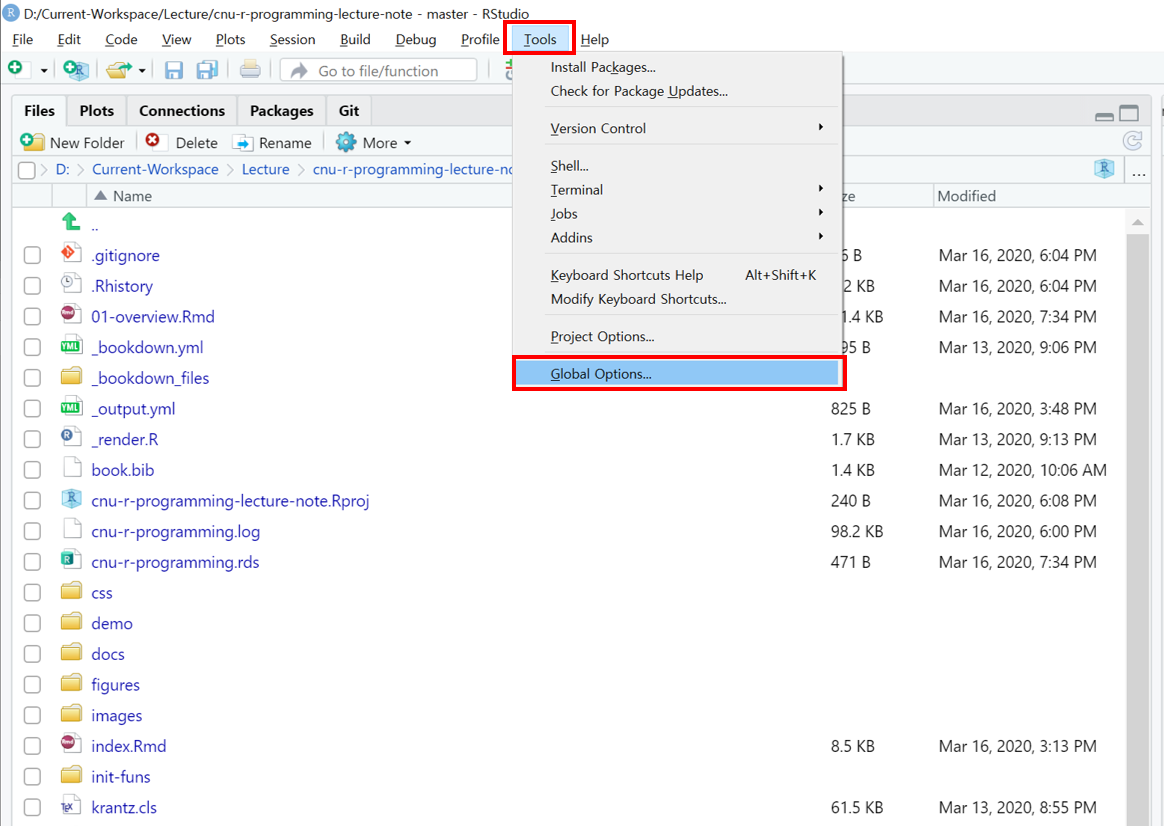
\includegraphics[width=0.8\linewidth]{figures/rstudio-glob-menu} \end{center}

\normalsize

\textbf{General}: RStudio 운용 관련 전반적 설정 세팅

\footnotesize

\begin{figure}

{\centering 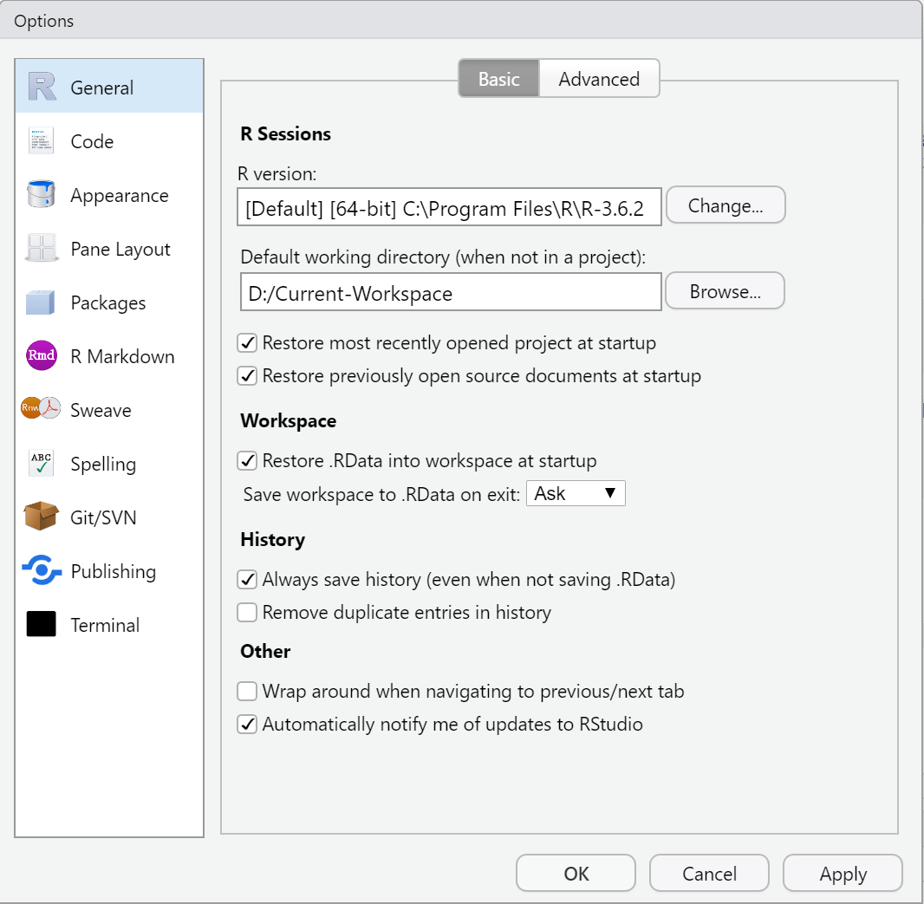
\includegraphics[width=0.8\linewidth]{figures/rstudio-glob-option} 

}

\caption{R General option 팝업 창}\label{fig:rstudio-glob-option}
\end{figure}

\normalsize

\begin{itemize}
\tightlist
\item
  \textbf{R version}: 만약 컴퓨터에 두 개 이상 다른 R 버전이 설치되어 있는 경우 \texttt{{[}Change{]}} 클릭 후 설정 변경 가능
\item
  \textbf{Default Working directory}: 작업 디렉토리 지정({[}\texttt{Browse}{]} 클릭 후 임의 폴더 설정 가능)
\item
  \textbf{Restore most recently opened project at startup}: RStudio 실행 시 가장 최근에 작업한 프로젝트로 이동
\item
  \textbf{Restore previously open source documents at startup}: RStudio 실행 시 현재 프로젝트에서 가장 최근에 작업한 소스코드 문서를 함께 열어줌.
\item
  \textbf{Restore .RData into workspace at startup}: 작업 디렉토리에 존재하는 \texttt{.RData} 파일을 RStudio 실행 시 불러옴
\item
  \textbf{Save workspace to .RData on exit}: R workspace 자동 저장(\texttt{.RData}) 여부
\item
  \textbf{Always save history (even when not saving .RData) }: R 실행 명령 history 저장 여부(Always/Never/Ask)
\item
  \textbf{Remove duplicate entries in history}: history 저장 시 중복 명령 제거 여부
\end{itemize}

작업폴더(Working Directory)는 현재 R session에서 사용하는 기본 폴더로서 R 소스파일 및 데이터의 저장 및 로딩시 기본이 되는 폴더임.

\begin{itemize}
\tightlist
\item
  소스파일이나 데이터를 불러들일 때 작업 폴더에 있는 파일은 경로명을 지정하지 않고 파일명만 사용해도 됨
\item
  작업폴더가 아닌 곳에 있는 파일을 불러들일 때는 경로명까지 써 주어야함.
\item
  R 데이터를 저장할때도 파일명만 쓰면 기본적으로 작업폴더에 저장되며, 다른 폴더에 저장하기 위해서는 경로명까지 써 주어야 함.
\end{itemize}

처음 컴퓨터에 RStudio를 설치하면 Working directory는 Windows 사용자 폴더(예: \texttt{user})의 \texttt{Document} 폴더가 기본값으로 설정되어 있음. 기본 작업폴더를 변경하려면 Figure \ref{fig:rstudio-glob-option}에서 설정 가능.

현재 R session의 작업 디렉토리 설정 방법

\begin{itemize}
\tightlist
\item
  \texttt{{[}Session{]}\ -\textgreater{}\ {[}Set\ Working\ Directoy{]}\ -\textgreater{}\ {[}Choose\ Directory{]}}에서 설정
\end{itemize}

\footnotesize

\begin{center}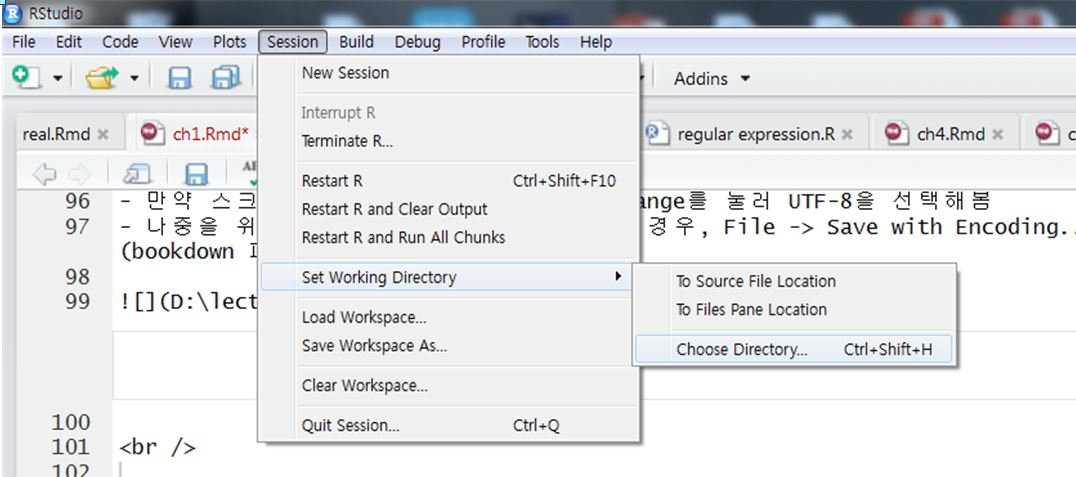
\includegraphics[width=0.8\linewidth]{figures/rstudio-wd-setting} \end{center}

\normalsize

R 콘솔에서 다음과 같은 명령어로 작업폴더를 확인 및 변경 가능

\footnotesize

\begin{Shaded}
\begin{Highlighting}[]
\KeywordTok{getwd}\NormalTok{() }\CommentTok{# 작업폴더 확인}
\end{Highlighting}
\end{Shaded}

\begin{verbatim}
[1] "D:/Current-Workspace/Lecture/cnu-r-programming-lecture-note"
\end{verbatim}

\normalsize

\footnotesize

\begin{Shaded}
\begin{Highlighting}[]
\KeywordTok{setwd}\NormalTok{(}\StringTok{".."}\NormalTok{) }\CommentTok{# 차상위 폴더로 이동}
\KeywordTok{getwd}\NormalTok{()}
\end{Highlighting}
\end{Shaded}

\begin{verbatim}
[1] "D:/Current-Workspace/Lecture"
\end{verbatim}

\begin{Shaded}
\begin{Highlighting}[]
\KeywordTok{setwd}\NormalTok{(}\StringTok{"../.."}\NormalTok{) }\CommentTok{# 차차상위 폴더로 이동}
\KeywordTok{getwd}\NormalTok{()}
\end{Highlighting}
\end{Shaded}

\begin{verbatim}
[1] "D:/"
\end{verbatim}

\begin{Shaded}
\begin{Highlighting}[]
\KeywordTok{setwd}\NormalTok{(}\StringTok{"D:/Current-Workspace/Lecture/misc/"}\NormalTok{) }\CommentTok{# 절대 폴더 명 입력}
\KeywordTok{setwd}\NormalTok{(}\StringTok{".."}\NormalTok{)}
\CommentTok{# dir() # 폴더 내 파일 명 출력}
\KeywordTok{getwd}\NormalTok{()}
\end{Highlighting}
\end{Shaded}

\begin{verbatim}
[1] "D:/Current-Workspace/Lecture"
\end{verbatim}

\begin{Shaded}
\begin{Highlighting}[]
\KeywordTok{setwd}\NormalTok{(}\StringTok{"misc"}\NormalTok{) }\CommentTok{# Current-Workspace 하위폴더인 misc 으로 이동}
\KeywordTok{getwd}\NormalTok{()}
\end{Highlighting}
\end{Shaded}

\begin{verbatim}
[1] "D:/Current-Workspace/Lecture/misc"
\end{verbatim}

\begin{Shaded}
\begin{Highlighting}[]
\KeywordTok{setwd}\NormalTok{(}\StringTok{"D:/Current-Workspace/Lecture/cnu-r-programming-lecture-note/"}\NormalTok{)}
\KeywordTok{getwd}\NormalTok{()}
\end{Highlighting}
\end{Shaded}

\begin{verbatim}
[1] "D:/Current-Workspace/Lecture/cnu-r-programming-lecture-note"
\end{verbatim}

\normalsize

\footnotesize

\begin{rmdcaution}
\begin{rmdcaution}

R에서 디렉토리 또는 폴더 구분자는 \texttt{/} 임. Windows에서 사용하는 구분자는 \texttt{\textbackslash{}}인데, R에서 \texttt{\textbackslash{}}는 특수문자로 간주하기 때문에 Windows 의 폴더명을 그대로 사용 시 에러 메세지를 출력함. 이를 해결하기 위해 Windows 경로명을 그대로 복사한 경우 경로 구분자 \texttt{\textbackslash{}} 대신 \texttt{\textbackslash{}\textbackslash{}}로 변경

\textbf{실습}: \texttt{C:\textbackslash{}r-project}를 컴퓨터에 생성 후 해당 폴더를 default 작업폴더로 설정

\end{rmdcaution}
\end{rmdcaution}

\normalsize

\textbf{Code: Editing}: 들여쓰기, 자동 줄바꿈 등 코드 편집에 대한 전반적 설정

\footnotesize

\begin{center}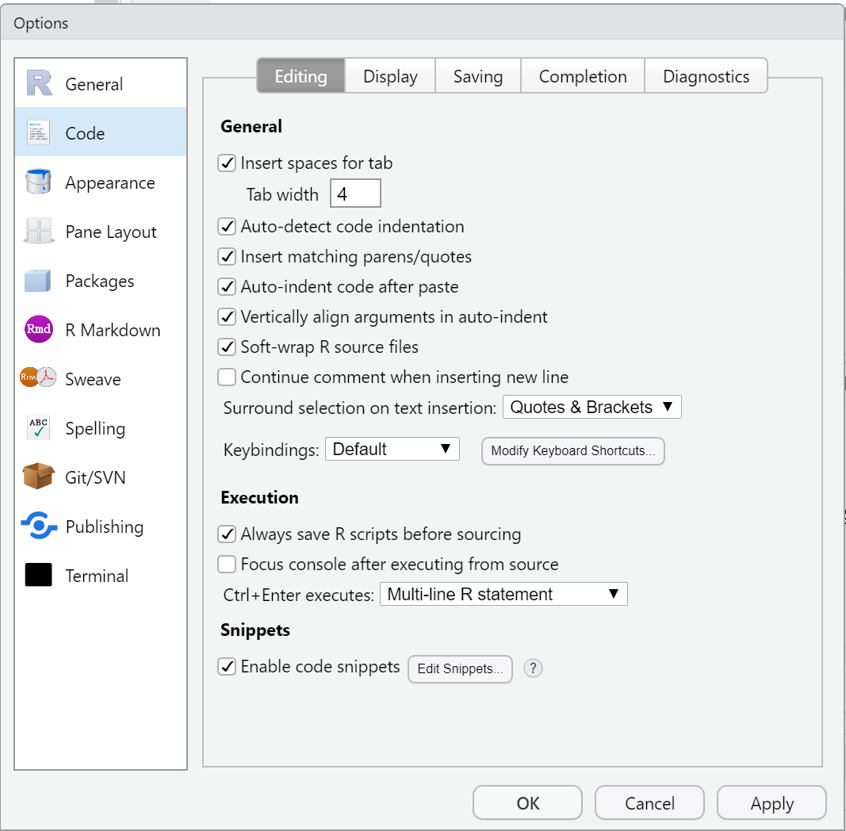
\includegraphics[width=0.8\linewidth]{figures/rstudio-code-edit-option} \end{center}

\normalsize

\begin{itemize}
\tightlist
\item
  \textbf{Insert spaces for tab}: \texttt{{[}Tab{]}} 키를 눌렀을 때 공백(space) 개수 결정(본 강의노트: \texttt{Tab\ width\ =\ 4})
\item
  \textbf{Auto-detect code indentation}: 코들 들여쓰기 자동 감지
\item
  \textbf{Insert matching parens/quotes}: 따옴표, 괄호 입력 시 커서를 따옴표/괄호 사이로 자동 이동
\item
  \textbf{Auto-indent code after paste}: 코드 복사 시 들여쓰기 일괄 적용
\item
  \textbf{Vertically align arguments in auto-indent}: 함수 작성 시 들여쓰기 레벨 유지 여부
\item
  \textbf{Soft-wrap R source file}: 스크립트 편집기 너비를 초과하는 경우 R 코드 행을 자동 줄바꿈
\item
  \textbf{Continue comment when inserting new line}: 주석 표시를 다음 행에도 자동 적용 여부
\item
  \textbf{Surround selection on text insertino}: 스크립트 상 text 선택 후 자동 따옴표 및 괄호 적용 여부
\item
  \textbf{Focus console after executing from source}: 스크립트 실행 후 커서 위치를 콘솔로 이동 여부
\end{itemize}

\textbf{Code: Display}: 스크립트(소스) 에디터 표시 화면 설정

\footnotesize

\begin{center}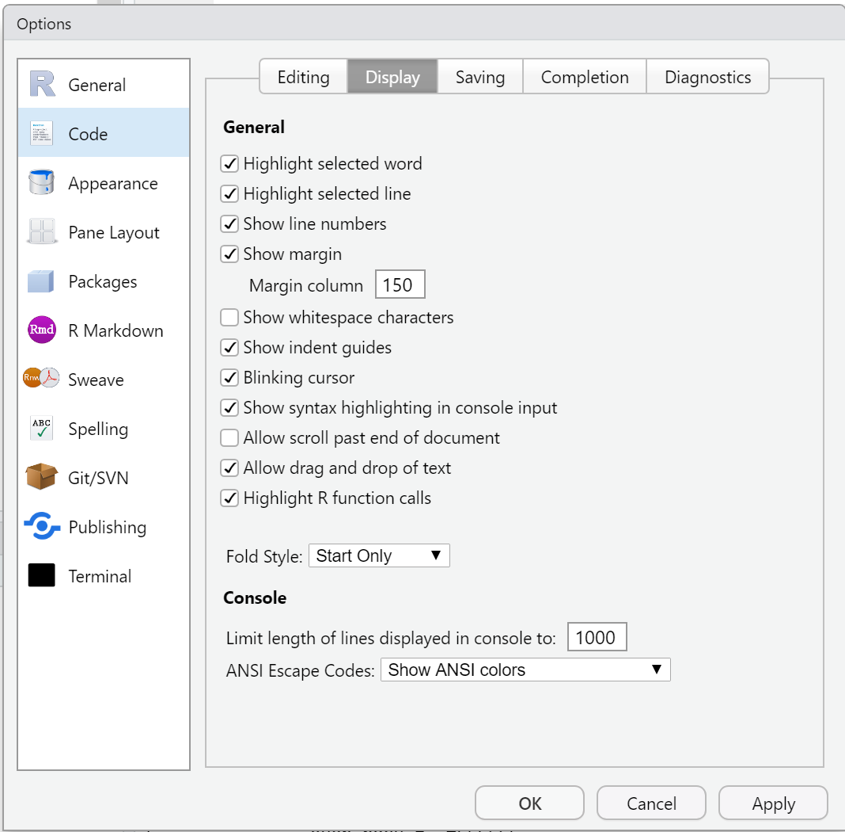
\includegraphics[width=0.8\linewidth]{figures/rstudio-code-display} \end{center}

\normalsize

\begin{itemize}
\tightlist
\item
  \textbf{Highlight selected word}: 스크립트 내 text 선택 시 동일한 text에 대해 배경강조 효과 여부
\item
  \textbf{Highlight selected line}: 선택된 행에 대해 배경 강조효과 여부
\item
  \textbf{Show line numbers}: 행 번호 보여주기 여부
\item
  \textbf{Show margin}: 소스 에디터 오른 쪽에 지정한 margin column 보여주기 여부
\item
  \textbf{Show whitespace characters}: 에디터에 공백 표시 여부
\item
  \textbf{Show indent guides}: 현재 들여쓰기 열 표시 여부
\item
  \textbf{Blinking cursor}: 커서 깜박임 여부
\item
  \textbf{Show syntax highlighting in console output}: 콘솔 입력 라인에 R 구문 강조 표시 적용 여부
\item
  \textbf{Allow scroll past end of document}: 문서 마지막 행 이후 스크롤 허용 여부
\item
  \textbf{Allow drag and drop of text}: 선택한 복수의 행으로 구성된 text에 대해 마우스 drag 허용
\item
  \textbf{Highlight R function calls}: R 내장 및 패키지 제공함수에 대해 강조 여부
\end{itemize}

\textbf{Code: Saving}: 스크립트(소스) 에디터 저장 설정

\footnotesize

\begin{center}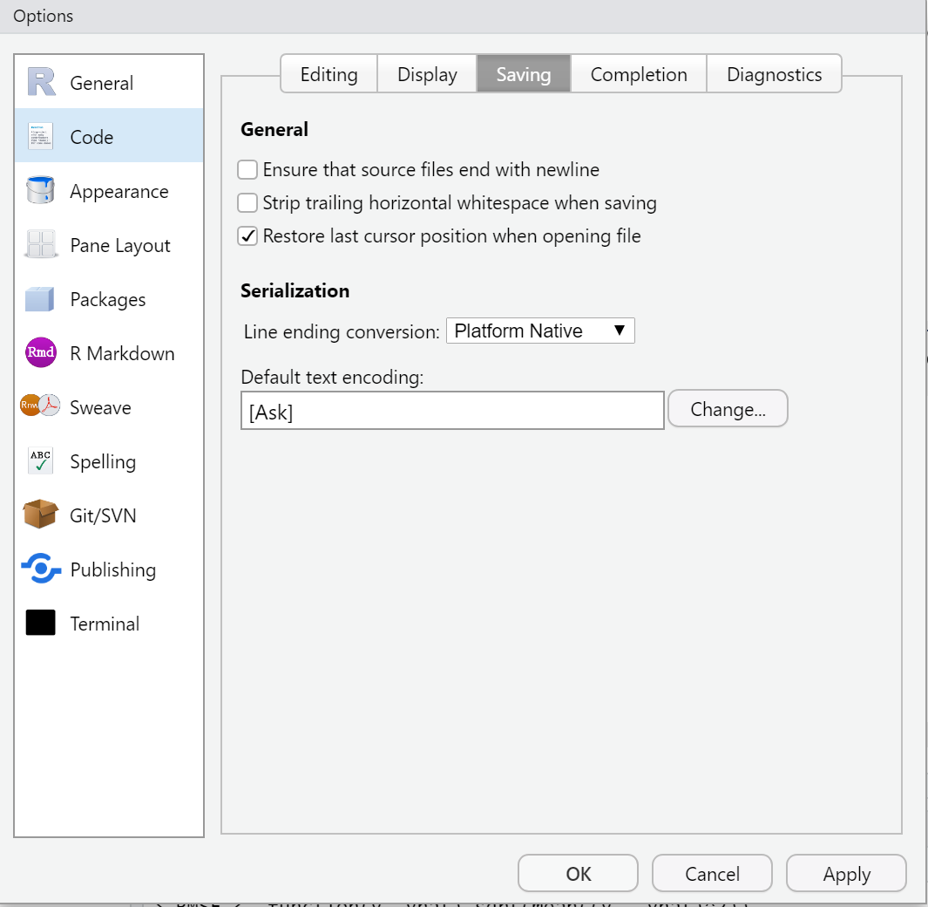
\includegraphics[width=0.8\linewidth]{figures/rstudio-code-saving} \end{center}

\normalsize

\begin{itemize}
\tightlist
\item
  \textbf{Ensure that source file end with newline}
\item
  \textbf{String trailing horizontal whitespace when saving}
\item
  \textbf{Restore last cursor position when opening file}
\item
  \textbf{Default text encoding}: 소스 에디터의 기본 설정 인코딩 설정 변경

  \begin{itemize}
  \tightlist
  \item
    RStudio의 Windows 버전 기본 text encoding은 \texttt{CP949} 임
  \item
    Linux나 Mac OS의 경우 한글은 \texttt{UTF-8}로 인코딩이 설정되어 있음.
  \item
    R 언어는 Linux 환경에서 개발되었기 때문에 \texttt{UTF-8} 인코딩과 호환성이 더 좋음
  \item
    스크립트 파일의 한글이 깨질 때는 \texttt{{[}File{]}\ -\textgreater{}\ {[}Reopen\ with\ Encoding...{]}}에서 encoding 방식 변경
  \end{itemize}
\end{itemize}

\textbf{Appearance}: RStudio 전체 폰트, 폰트 크기, theme 설정

\footnotesize

\begin{center}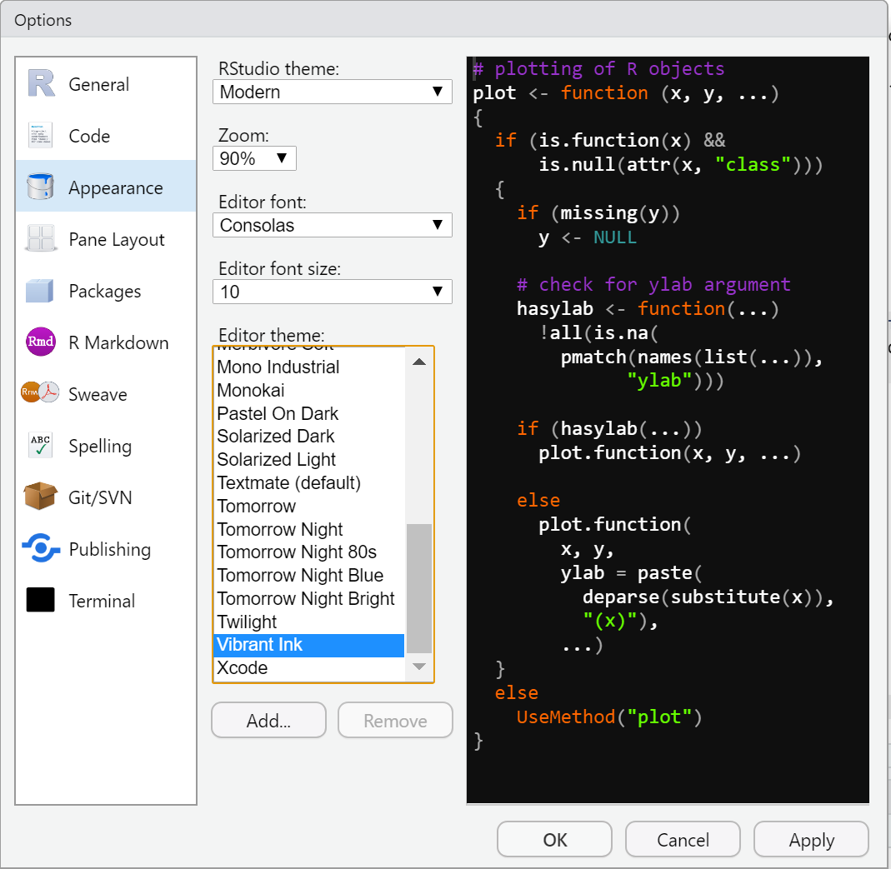
\includegraphics[width=0.8\linewidth]{figures/rstudio-appearance} \end{center}

\normalsize

\begin{itemize}
\tightlist
\item
  본인의 취향에 맞게 폰트 및 테마(theme) 설정
\item
  취향 \(\rightarrow\) 가독성이 제일 좋고 편안한 theme
\end{itemize}

\textbf{Pane Layout}: RStudio 구성 패널들의 위치 및 항목 등을 수정/추가/삭제(4개 페널은 항시 유지)

\footnotesize

\begin{center}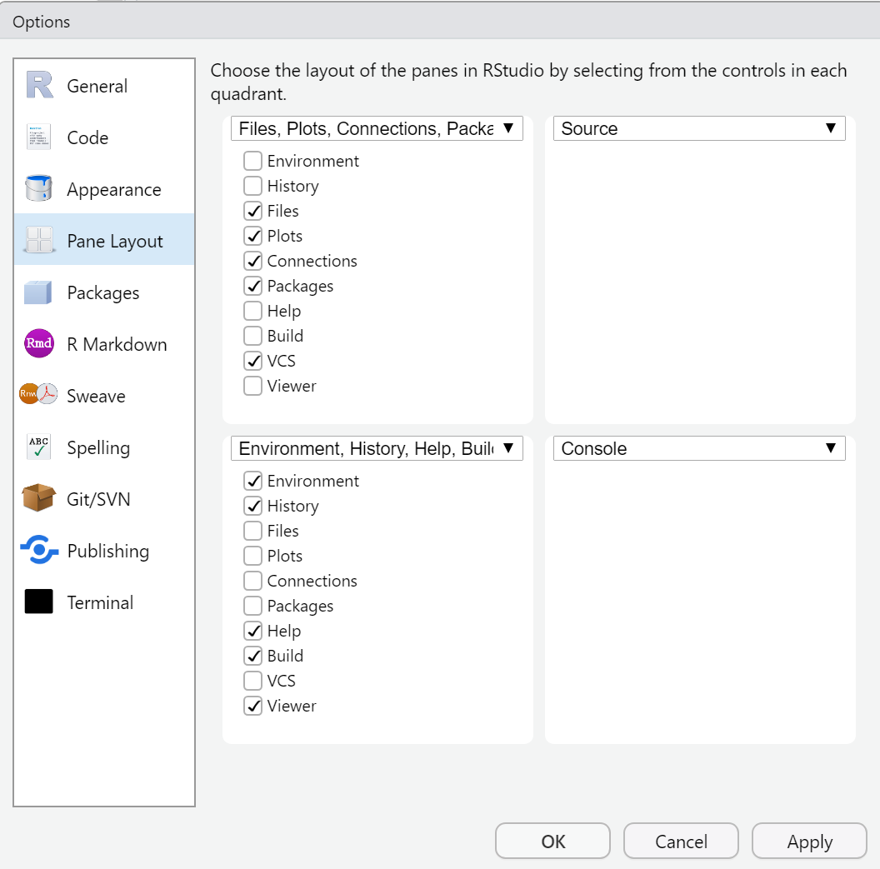
\includegraphics[width=0.8\linewidth]{figures/rstudio-pane-layout} \end{center}

\normalsize

\footnotesize

\begin{rmdimportant}
\begin{rmdimportant}

\textbf{실습}: 개인 취향에 맞게 RStudio 에디터 및 theme을 변경해 보자!!

\end{rmdimportant}
\end{rmdimportant}

\normalsize

\hypertarget{rstudio-project}{%
\subsection{RStudio 프로젝트}\label{rstudio-project}}

\begin{enumerate}
\def\labelenumi{\arabic{enumi}.}
\tightlist
\item
  프로젝트

  \begin{itemize}
  \tightlist
  \item
    물리적 측면: 최종 산출물(문서)를 생성하기 위한 데이터, 사진, 그림 등을 모아 놓은 폴더
  \item
    논리적 측면: R session 및 작업의 버전 관리
  \end{itemize}
\item
  프로젝트의 필요성

  \begin{itemize}
  \tightlist
  \item
    자료의 정합성 보장
  \item
    다양한 확장자를 갖는 파일들이 한 폴더 내에 뒤섞일 때 곤란해 질 수 있음
  \item
    실제 분석 및 그래프 생성에 사용한 정확한 프로그램 또는 코드 연결이 어려움
  \end{itemize}
\item
  좋은 프로젝트 구성을 위한 방법

  \begin{itemize}
  \tightlist
  \item
    원자료(raw data)의 보호: 가급적 자료를 읽기 전용(read only) 형태로 다루기
  \item
    데이터 정제(data wrangling 또는 data munging)를 위한 스크립트와 정제 자료를 보관하는 읽기 전용 데이터 디렉토리 생성
  \item
    작성한 스크립트로 생성한 모든 산출물(테이블, 그래프 등)을 ``일회용품''처럼 처리 \(\rightarrow\) 스크립트로 재현 가능
  \item
    한 프로젝트 내 각기 다른 분석마다 다른 하위 디렉토리에 출력결과 저장하는 것이 유용
  \end{itemize}
\item
  RStudio 새로운 프로젝트 생성

  \begin{itemize}
  \tightlist
  \item
    RStudio의 강력하고 유용한 기능
  \item
    새로운 프로젝트 생성: RStudio 메뉴에서 \texttt{{[}File{]}} \(\rightarrow\) \texttt{{[}New\ Project{]}} 선택하면 아래와 같은 팝업 메뉴 생성
  \end{itemize}
\end{enumerate}

\footnotesize

\begin{center}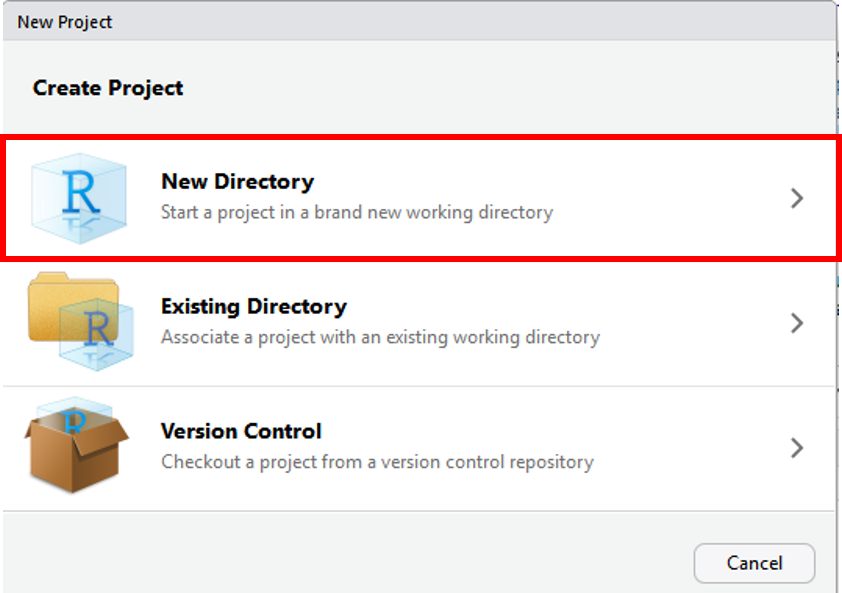
\includegraphics[width=0.8\linewidth]{figures/R-newproject-01} \end{center}

\normalsize

\begin{enumerate}
\def\labelenumi{\arabic{enumi}.}
\setcounter{enumi}{3}
\tightlist
\item
  위 그림에서 \texttt{New\ Directory}를 선택하면 아래와 같은 팝업 창이 나타나면 아래와 같은 프로젝트 유형이 나타남. 여기서는 \texttt{New\ Project} 선택
\end{enumerate}

\footnotesize

\begin{center}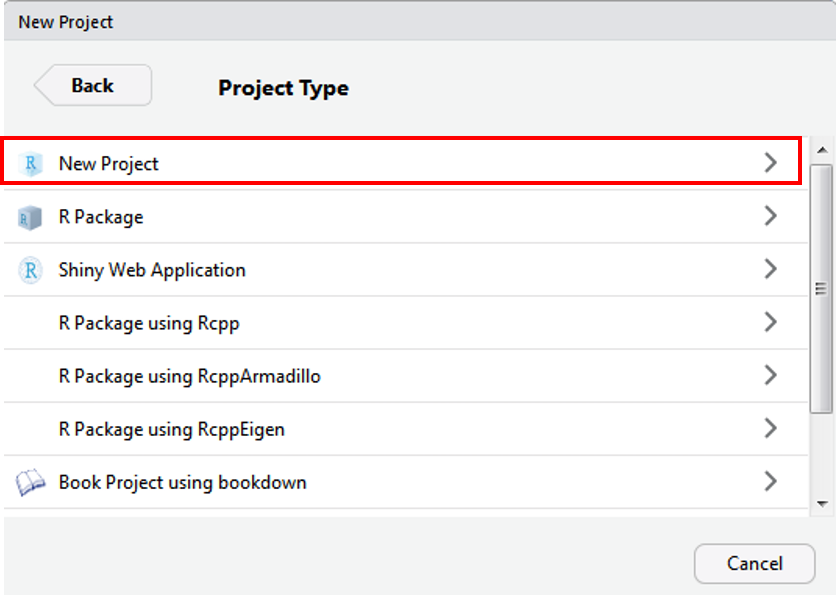
\includegraphics[width=0.8\linewidth]{figures/R-newproject-02} \end{center}

\normalsize

\begin{enumerate}
\def\labelenumi{\arabic{enumi}.}
\setcounter{enumi}{4}
\tightlist
\item
  다음 팝업창에서 새로운 프로젝트의 폴더명을 지정 후 \texttt{Create\ Project} 클릭

  \begin{itemize}
  \tightlist
  \item
    아래 \texttt{{[}Create\ projects\ as\ subdirectories\ of{]}}에서 생성하고자 하는 프로젝트의 상위 디렉토리 설정 \(\rightarrow\) 보통 RStudio의 기본 작업폴더로 설정
  \end{itemize}
\end{enumerate}

\footnotesize

\begin{center}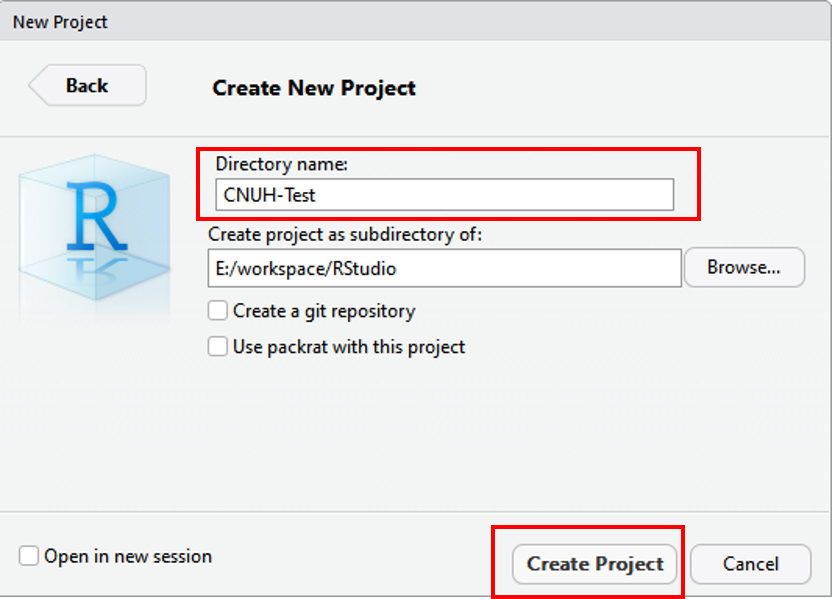
\includegraphics[width=0.8\linewidth]{figures/R-newproject-03} \end{center}

\normalsize

\begin{enumerate}
\def\labelenumi{\arabic{enumi}.}
\setcounter{enumi}{5}
\tightlist
\item
  현재 R session 종료 후 새로운 프로젝트로 session 화면이 열리면 프로젝트 생성 완료
\end{enumerate}

\footnotesize

\begin{rmdimportant}
\begin{rmdimportant}

\textbf{실습}: 프로젝트 생성

\begin{itemize}
\tightlist
\item
  위에서 설정한 작업폴더 내에 \texttt{학번-r-programming} 프로젝트 생성
\item
  생성한 프로젝트 폴더 내에 \texttt{docs}, \texttt{figures}, \texttt{script} 폴더 생성
\end{itemize}

\end{rmdimportant}
\end{rmdimportant}

\normalsize

\hypertarget{r-package}{%
\section{R 패키지}\label{r-package}}

\footnotesize

\begin{rmdnote}
\begin{rmdnote}

\textbf{R 패키지(package)}: 특수 목적을 위한 로직으로 구성된 코드들의 집합으로 R에서 구동되는 분석툴을 통칭

\begin{itemize}
\tightlist
\item
  CRAN을 통해 배포: 3자가 이용하기 쉬움 \(\rightarrow\) R 시스템 환경에서 패키지는 가장 중요한 역할
\item
  CRAN \href{https://cran.r-project.org/web/packages/available_packages_by_date.html}{available package by name} 또는 \href{https://cran.r-project.org/web/packages/available_packages_by_name.html}{available package by date}에서 현재 등재된 패키지 리스트 확인 가능
\item
  R console에서 \texttt{available.packages()} 함수를 통해서도 확인 가능
\item
  현재 CRAN 기준(2020-03-17) 배포된 패키지의 개수는 16045 개임
\end{itemize}

\textbf{목적}: RStudio 환경에서 패키지를 설치하고 불러오기

\end{rmdnote}
\end{rmdnote}

\normalsize

\hypertarget{r-package-path}{%
\subsection{R 패키지 경로 확인 및 변경}\label{r-package-path}}

\begin{itemize}
\tightlist
\item
  패키지 설치 시 일반적으로 R 환경에서 기본값으로 지정한 라이브러리 폴더에 저장
\item
  패키지 설치 전 R 패키지 설치 경로(path) 지정
\item
  \texttt{.libPaths()} 함수를 통해 현재 설정된 패키지 저장 경로 확인
\end{itemize}

\footnotesize

\begin{Shaded}
\begin{Highlighting}[]
\KeywordTok{.libPaths}\NormalTok{()}
\end{Highlighting}
\end{Shaded}

\begin{verbatim}
[1] "C:/Users/user/Documents/R/win-library/4.0"
[2] "C:/Program Files/R/R-4.0.0/library"       
\end{verbatim}

\normalsize

\begin{itemize}
\tightlist
\item
  일반적으로 첫 번째 경로를 디폴트 라이브러리 폴더로 사용
\item
  사용자 지정 라이브러리 경로를 설정 하려면 아래와 같은 절차로 진행
\end{itemize}

\begin{quote}
\textbf{실습: c:/r-library 폴더를 패키지 경로로 지정}
\end{quote}

\begin{enumerate}
\def\labelenumi{\arabic{enumi})}
\item
  \texttt{C:\textbackslash{}}에서 {[}새로 만들기(W){]} -\textgreater{} {[}폴더(F){]} 선택 후 생성 폴더 이름을 \texttt{r-library}로 변경
\item
  윈도우즈 \texttt{{[}제어판{]}\ -\textgreater{}\ {[}시스템\ 및\ 보안{]}\ -\textgreater{}\ {[}시스템{]}\ -\textgreater{}\ {[}고급\ 시스템\ 설정{]}} 클릭
\end{enumerate}

\footnotesize

\begin{center}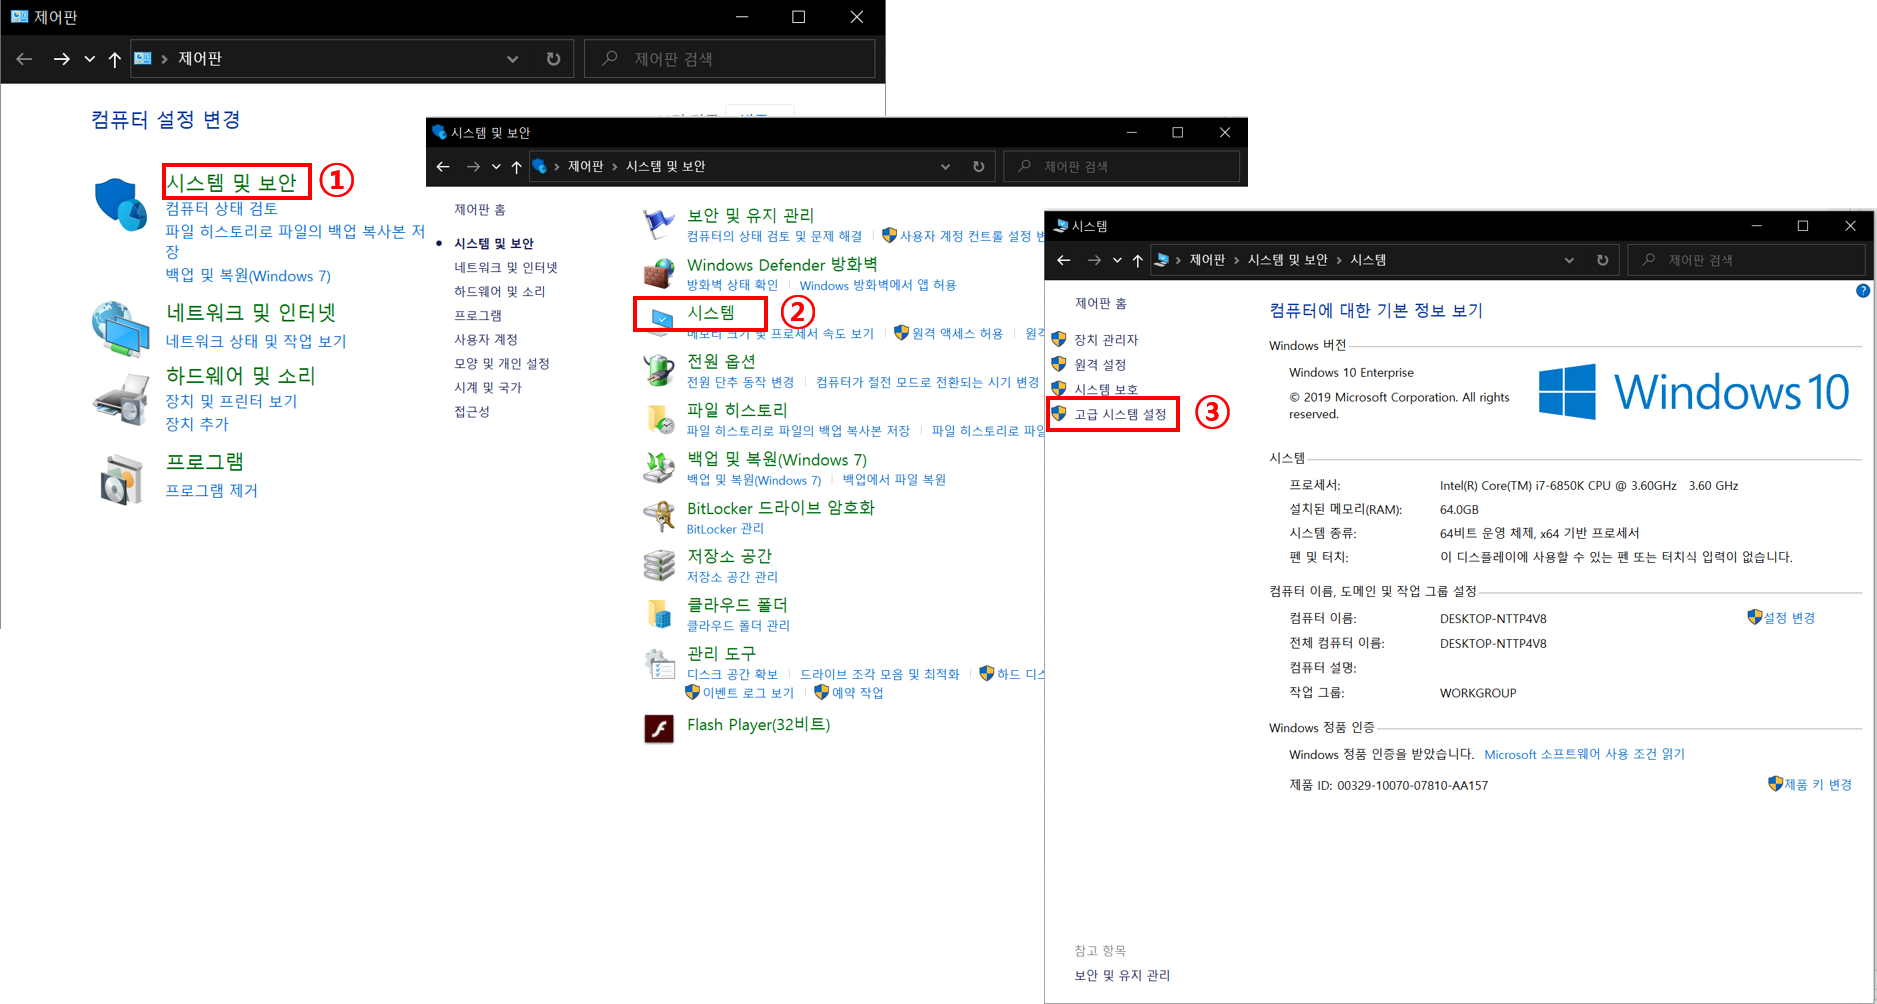
\includegraphics[width=0.8\linewidth]{figures/window-env-system} \end{center}

\normalsize

\begin{enumerate}
\def\labelenumi{\arabic{enumi})}
\setcounter{enumi}{2}
\tightlist
\item
  \texttt{{[}환경변수(N)...{]}} 선택 후 시스템 변수에서 \texttt{{[}새로\ 만들기(W)...{]}} 클릭
\end{enumerate}

\footnotesize

\begin{center}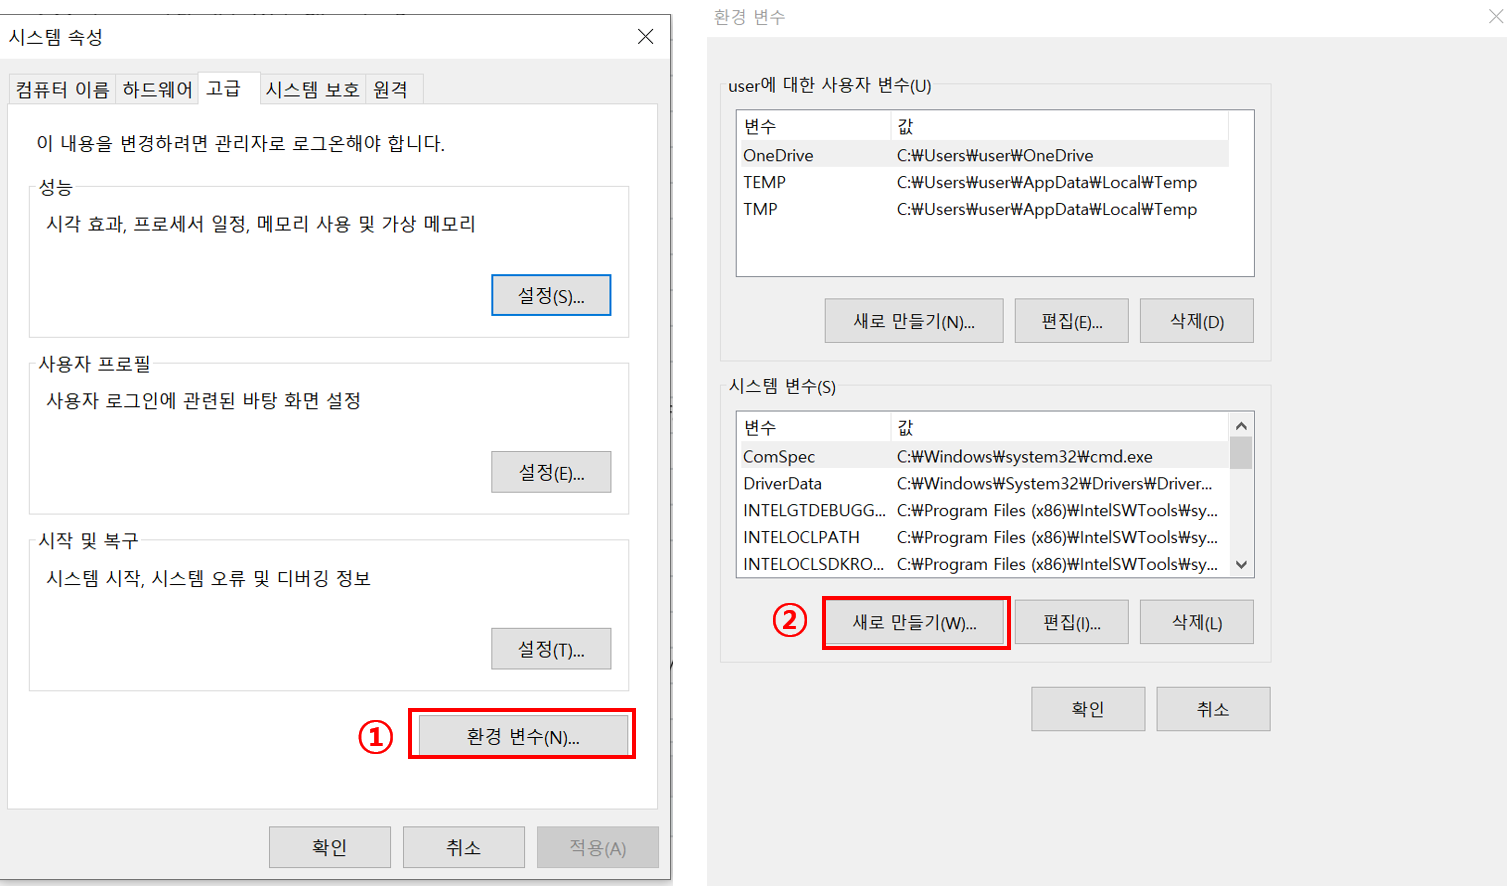
\includegraphics[width=0.8\linewidth]{figures/window-env-var} \end{center}

\normalsize

\begin{enumerate}
\def\labelenumi{\arabic{enumi})}
\setcounter{enumi}{3}
\tightlist
\item
  아래 그림과 같이 변수 이름(N)에 \texttt{R\_LIBS}, 변수 값(V)에 해당 디렉토리 경로 \texttt{C:\textbackslash{}r-library} 입력 후 확인 버튼 클릭
\end{enumerate}

\footnotesize

\begin{center}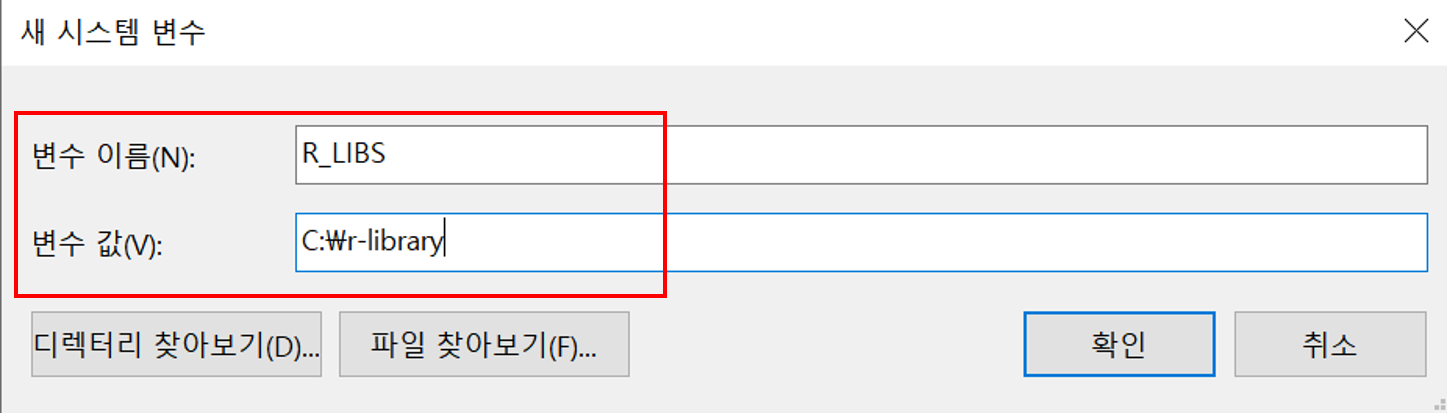
\includegraphics[width=0.9\linewidth]{figures/window-new-system-var} \end{center}

\normalsize

\begin{enumerate}
\def\labelenumi{\arabic{enumi})}
\setcounter{enumi}{4}
\tightlist
\item
  현재 RStudio 종료 후 재실행한 다음 콘솔창에 \texttt{.libPaths()} 입력 후 라이브러리 경로 확인
\end{enumerate}

\hypertarget{r-package-install}{%
\subsection{R 패키지 설치하기}\label{r-package-install}}

\begin{itemize}
\tightlist
\item
  RStudio 메뉴 \texttt{{[}Tools{]}} \(\rightarrow\) \texttt{{[}Install\ packages{]}} 클릭 후 생성된 팝업 창에서 설치하고자 하는 패키지 입력 후 설치
\end{itemize}

\footnotesize

\begin{center}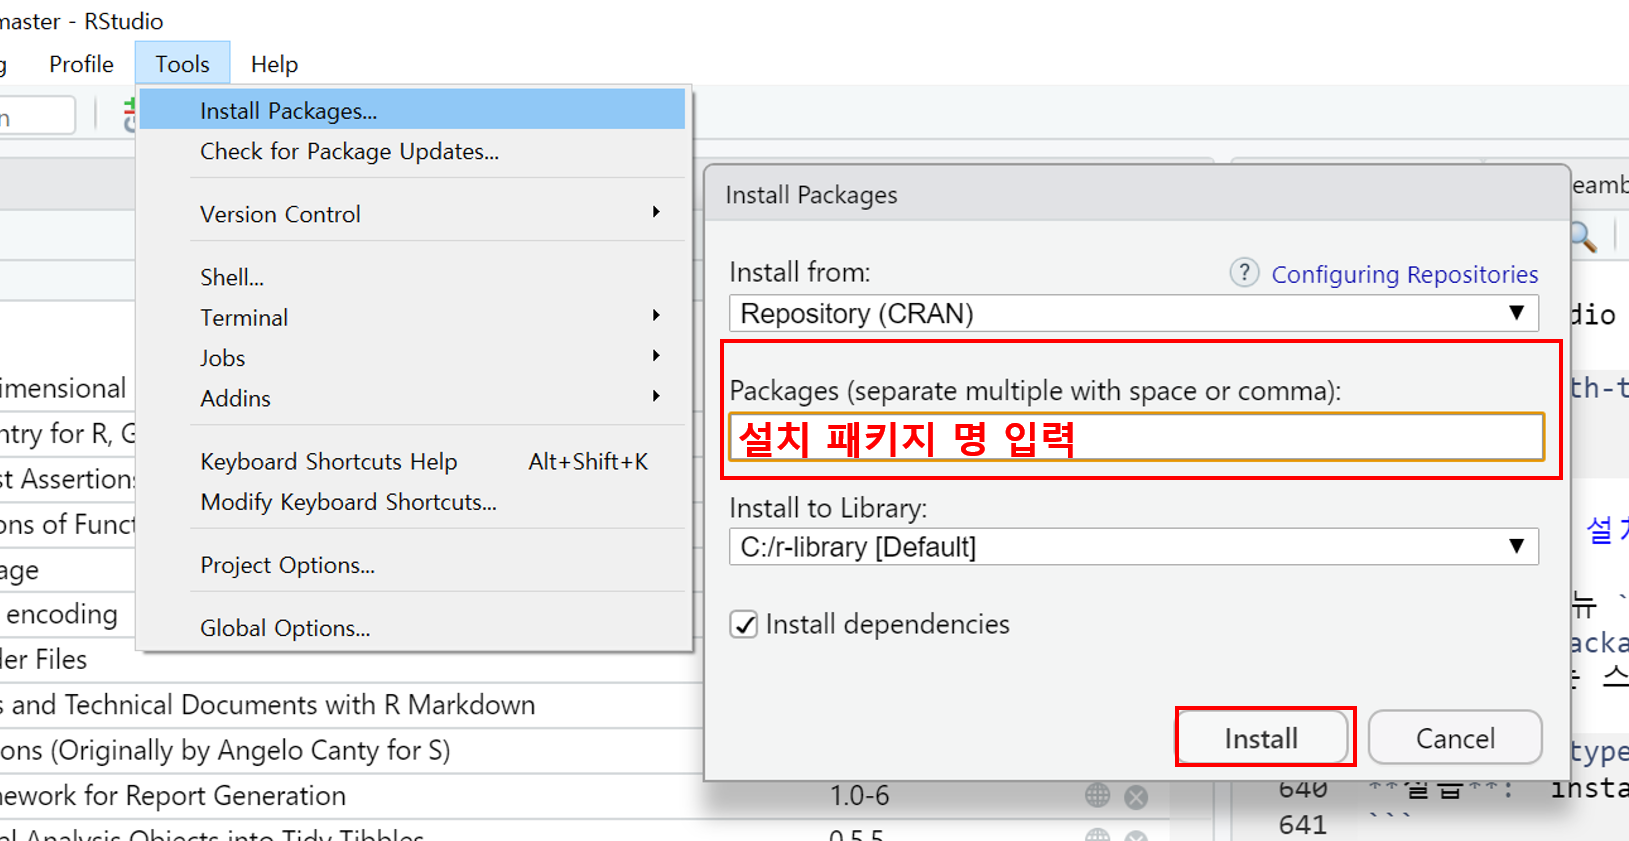
\includegraphics[width=0.8\linewidth]{figures/rstudio-package-install} \end{center}

\normalsize

\begin{itemize}
\tightlist
\item
  RStudio \texttt{Packages} 창에서 \texttt{{[}Install{]}} 버튼 누르면 위와 동일한 팝업창이 나타남(위와 동일)
\end{itemize}

\footnotesize

\begin{center}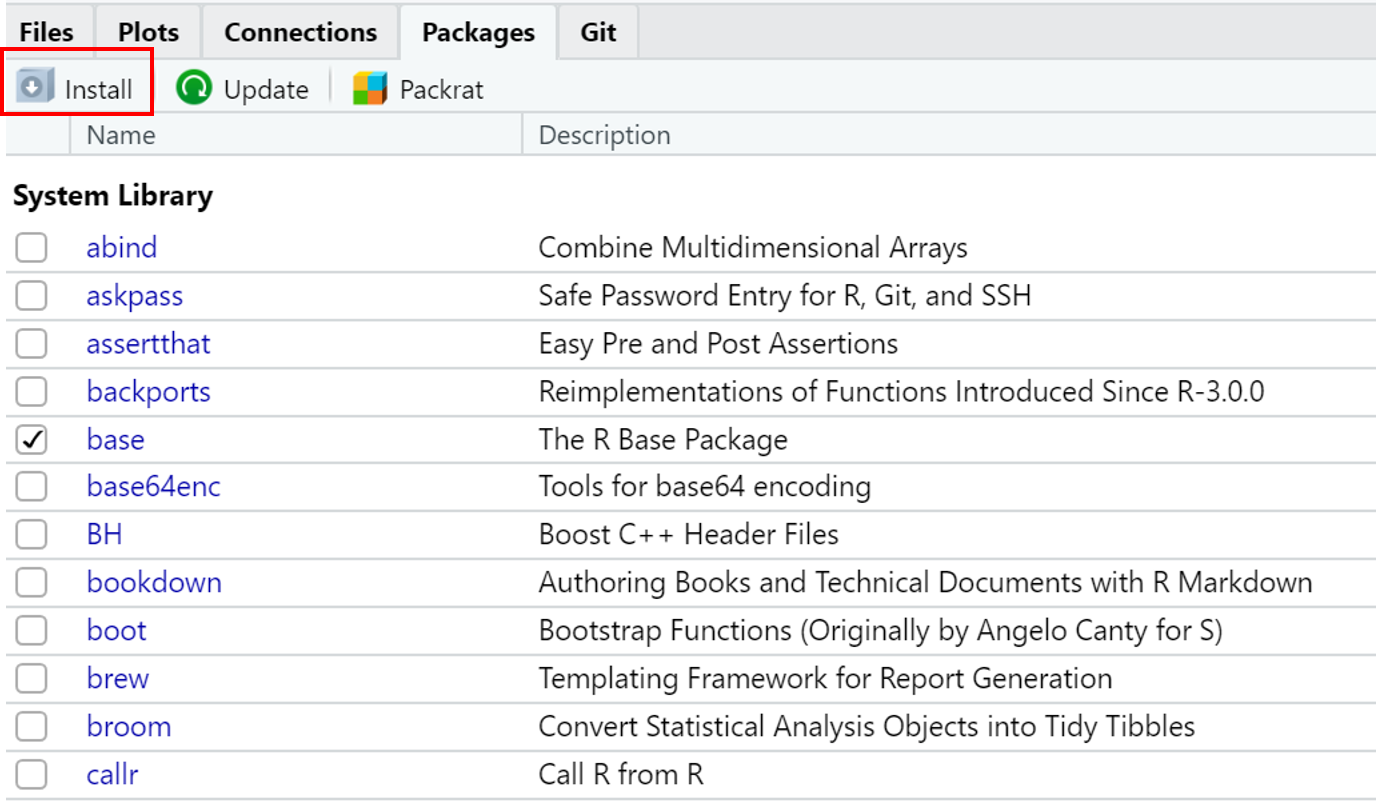
\includegraphics[width=0.8\linewidth]{figures/rstudio-pack-win-02} \end{center}

\normalsize

\begin{itemize}
\tightlist
\item
  R 콘솔 또는 스크립트 창에서 \texttt{install.packages(package\_name)} 함수를 사용해서 패키지 설치
\end{itemize}

\footnotesize

\begin{rmdimportant}
\begin{rmdimportant}

\textbf{실습}: \texttt{install.packages()} 함수를 이용해 \texttt{tidyverse} 패키지 설치

\end{rmdimportant}
\end{rmdimportant}

\normalsize

\footnotesize

\begin{Shaded}
\begin{Highlighting}[]
\KeywordTok{install.packages}\NormalTok{(}\StringTok{"tidyverse"}\NormalTok{)}
\end{Highlighting}
\end{Shaded}

\normalsize

\begin{quote}
위 명령어를 실행하면 \texttt{tidyverse} 패키지 뿐 아니라 연관된 패키지들이 동시에 설치됨
\end{quote}

\hypertarget{r-package-load}{%
\subsection{R 패키지 불러오기}\label{r-package-load}}

\begin{enumerate}
\def\labelenumi{\arabic{enumi}.}
\tightlist
\item
  \texttt{library()} vs.~\texttt{require()}

  \begin{itemize}
  \tightlist
  \item
    \texttt{library()}: 불러오고자 하는 패키지가 시스템에 존재하지 않는 경우 에러 메세지 출력(에러 이후 명령어들이 실행되지 않음)
  \item
    \texttt{require()}: 패키지가 시스템에 존재하지 않는 경우 경고 메세지 출력(경고 이후 명령어 정상적으로 실행)
  \end{itemize}
\item
  다중 패키지 동시에 불러오기

  \begin{itemize}
  \tightlist
  \item
    RStudio \texttt{Packages} 창에서 설치하고자 하는 패키지 선택 버튼 클릭하면 R workspace로 해당 패키지 로드 가능
  \item
    스크립트 이용
  \end{itemize}
\end{enumerate}

\footnotesize

\begin{rmdimportant}
\begin{rmdimportant}

\textbf{실습}: \texttt{tidyverse} 패키지 불러오기

\end{rmdimportant}
\end{rmdimportant}

\normalsize

\footnotesize

\begin{Shaded}
\begin{Highlighting}[]
\KeywordTok{require}\NormalTok{(tidyverse)}
\end{Highlighting}
\end{Shaded}

\begin{verbatim}
필요한 패키지를 로딩중입니다: tidyverse
\end{verbatim}

\begin{verbatim}
-- Attaching packages ------------------------------------------------------------------------------------------------------------- tidyverse 1.3.0 --
\end{verbatim}

\begin{verbatim}
v ggplot2 3.3.1     v purrr   0.3.4
v tibble  3.0.1     v dplyr   1.0.0
v tidyr   1.1.0     v stringr 1.4.0
v readr   1.3.1     v forcats 0.5.0
\end{verbatim}

\begin{verbatim}
-- Conflicts ---------------------------------------------------------------------------------------------------------------- tidyverse_conflicts() --
x dplyr::filter()     masks stats::filter()
x dplyr::group_rows() masks kableExtra::group_rows()
x dplyr::lag()        masks stats::lag()
\end{verbatim}

\normalsize

\footnotesize

\begin{rmdnote}
\begin{rmdnote}

실무에서 R의 활용능력은 패키지 활용 여부에 달려 있음. 즉, 목적에 맞는 업무를 수행하기 위해 가장 적합한 패키지를 찾고 활용하느냐에 따라 R 활용능력의 차이를 보임. 앞서 언급한 바와 같이 CRAN에 등록된 패키지는 16000 개가 넘지만, 이 중 많이 활용되고 있는 패키지의 수는 약 200 \textasciitilde{} 300 개 내외이고, 실제 데이터 분석 시 10 \textasciitilde{} 20개 정도의 패키지가 사용됨. 앞 예제에서 설치하고 불러온 \texttt{tidyverse} 패키지는 Hadley Wickham \citep{tidyverse2019}이 개발한 데이터 전처리 및 시각화 패키지 번들이고, 현재 R 프로그램 환경에 지대한 영향을 미침. 본 강의 ``데이터프레임 가공 및 시각화''에서 해당 패키지 활용 방법을 배울 예정

\end{rmdnote}
\end{rmdnote}

\normalsize

\hypertarget{r-basic}{%
\section{R 기초 문법}\label{r-basic}}

\footnotesize

\begin{rmdnote}
\begin{rmdnote}

본 절에서 다루는 R 문법은 R 입문 시 객체(object)의 명명 규칙과 R 콘솔 창에서 가장 빈번하게 사용되는 기초적인 명령어만 다룰 예정임. 심화 내용은 2-3주 차에 다룰 예정임.

\end{rmdnote}
\end{rmdnote}

\normalsize

\begin{itemize}
\tightlist
\item
  R은 객체지향언어(object-oriented language)

  \begin{itemize}
  \tightlist
  \item
    객체(object): 숫자, 데이터셋, 단어, 테이블, 분석결과 등 모든 것을 칭함
  \item
    ``객체지향''의 의미는 R의 모든 명령어는 객체를 대상으로 이루어진다는 것을 의미
  \end{itemize}
\end{itemize}

\footnotesize

\begin{rmdtip}
\begin{rmdtip}

알아두면 유용한(콘솔창에서 매우 많이 사용되는) 명령어 및 단축키

\begin{itemize}
\tightlist
\item
  \texttt{ls()}: 현재 R 작업공간에 저장된 모든 객체 리스트 출력
\item
  \texttt{rm(object\_name)}: \texttt{object\_name}에 해당하는 객체 삭제
\item
  \texttt{rm(list\ =\ ls())}: R 작업공간에 저장된 모든 객체들을 일괄 삭제
\item
  단축키 \texttt{{[}Ctrl{]}\ +\ {[}L{]}}: R 콘솔 창 일괄 청소
\item
  단축키 \texttt{{[}Ctrl{]}\ +\ {[}Shift{]}\ +\ {[}F10{]}}: R session 초기화
\end{itemize}

\textbf{예시}

\end{rmdtip}
\end{rmdtip}

\normalsize

\footnotesize

\begin{Shaded}
\begin{Highlighting}[]
\NormalTok{x <-}\StringTok{ }\DecValTok{7}
\NormalTok{y <-}\StringTok{ }\DecValTok{1}\OperatorTok{:}\DecValTok{30} \CommentTok{#1에서 30까지 정수 입력}
\KeywordTok{ls}\NormalTok{() }\CommentTok{#현재 작업공간 내 객체명 출력}
\end{Highlighting}
\end{Shaded}

\begin{verbatim}
 [1] "a"                  "b"                  "cars"              
 [4] "def.chunk.hook"     "fig_cap"            "hook_output"       
 [7] "tab"                "x"                  "y"                 
[10] "도움말 보기 명령어" "사용법"             "설명"              
\end{verbatim}

\normalsize

\footnotesize

\begin{Shaded}
\begin{Highlighting}[]
\KeywordTok{rm}\NormalTok{(x) }\CommentTok{# 객체 x 삭제}
\KeywordTok{ls}\NormalTok{()}
\end{Highlighting}
\end{Shaded}

\begin{verbatim}
 [1] "a"                  "b"                  "cars"              
 [4] "def.chunk.hook"     "fig_cap"            "hook_output"       
 [7] "tab"                "y"                  "도움말 보기 명령어"
[10] "사용법"             "설명"              
\end{verbatim}

\begin{Shaded}
\begin{Highlighting}[]
\KeywordTok{rm}\NormalTok{(a,b) }\CommentTok{# 객체 a,b 동시 삭제}
\KeywordTok{ls}\NormalTok{()}
\end{Highlighting}
\end{Shaded}

\begin{verbatim}
[1] "cars"               "def.chunk.hook"     "fig_cap"           
[4] "hook_output"        "tab"                "y"                 
[7] "도움말 보기 명령어" "사용법"             "설명"              
\end{verbatim}

\begin{Shaded}
\begin{Highlighting}[]
\CommentTok{# rm(list = ls()) # 모든 객체 삭제}
\end{Highlighting}
\end{Shaded}

\normalsize

\hypertarget{r-object-nam-rule}{%
\subsubsection*{R 객체 입력 방법 및 변수 설정 규칙}\label{r-object-nam-rule}}


객체를 할당하는 두 가지 방법:\texttt{=}, \texttt{\textless{}-}

\begin{itemize}
\tightlist
\item
  두 할당 지시자의 차이점

  \begin{itemize}
  \tightlist
  \item
    \texttt{=}: 명령의 최상 수준에서만 사용 가능
  \item
    \texttt{\textless{}-}: 어디서든 사용 가능
  \item
    함수 호출과 동시에 변수에 값을 할당할 목적으로는 \texttt{\textless{}-}만 사용 가능
  \end{itemize}
\end{itemize}

\footnotesize

\begin{Shaded}
\begin{Highlighting}[]
\CommentTok{# mean(): 입력 벡터의 평균 계산}
\KeywordTok{mean}\NormalTok{(y <-}\StringTok{ }\DecValTok{1}\OperatorTok{:}\DecValTok{5}\NormalTok{)}
\end{Highlighting}
\end{Shaded}

\begin{verbatim}
[1] 3
\end{verbatim}

\begin{Shaded}
\begin{Highlighting}[]
\NormalTok{y}
\end{Highlighting}
\end{Shaded}

\begin{verbatim}
[1] 1 2 3 4 5
\end{verbatim}

\begin{Shaded}
\begin{Highlighting}[]
\KeywordTok{mean}\NormalTok{(}\DataTypeTok{x =} \DecValTok{1}\OperatorTok{:}\DecValTok{5}\NormalTok{)}
\end{Highlighting}
\end{Shaded}

\begin{verbatim}
[1] 3
\end{verbatim}

\begin{Shaded}
\begin{Highlighting}[]
\NormalTok{x}
\end{Highlighting}
\end{Shaded}

\begin{verbatim}
Error in eval(expr, envir, enclos): 객체 'x'를 찾을 수 없습니다
\end{verbatim}

\normalsize

객체 또는 변수의 명명 규칙

\begin{itemize}
\tightlist
\item
  알파벳, 한글, 숫자, \texttt{\_}, \texttt{.}의 조합으로 구성 가능(\texttt{-}은 사용 불가)
\item
  변수명의 알파벳, 한글, \texttt{.}로 시작 가능
\item
  \texttt{.}로 시작한 경우 뒤에 숫자 올 수 없음(숫자로 인지)
\item
  대소문자 구분
\end{itemize}

\footnotesize

\begin{Shaded}
\begin{Highlighting}[]
\CommentTok{# 1:10은 1부터 10까지 정수 생성}
\CommentTok{# 'c()'는 벡터 생성 함수}
\NormalTok{x <-}\StringTok{ }\KeywordTok{c}\NormalTok{(}\DecValTok{1}\OperatorTok{:}\DecValTok{10}\NormalTok{) }
\CommentTok{# 1:10으로 구성된 행렬 생성}
\NormalTok{X <-}\StringTok{ }\KeywordTok{matrix}\NormalTok{(}\KeywordTok{c}\NormalTok{(}\DecValTok{1}\OperatorTok{:}\DecValTok{10}\NormalTok{), }\DataTypeTok{nrow =} \DecValTok{2}\NormalTok{, }\DataTypeTok{ncol =} \DecValTok{5}\NormalTok{, }\DataTypeTok{byrow =}\NormalTok{ T)}
\NormalTok{x}
\end{Highlighting}
\end{Shaded}

\begin{verbatim}
 [1]  1  2  3  4  5  6  7  8  9 10
\end{verbatim}

\begin{Shaded}
\begin{Highlighting}[]
\NormalTok{X}
\end{Highlighting}
\end{Shaded}

\begin{verbatim}
     [,1] [,2] [,3] [,4] [,5]
[1,]    1    2    3    4    5
[2,]    6    7    8    9   10
\end{verbatim}

\begin{Shaded}
\begin{Highlighting}[]
\CommentTok{# 논리형 객체}
\NormalTok{.x <-}\StringTok{ }\OtherTok{TRUE}
\NormalTok{.x}
\end{Highlighting}
\end{Shaded}

\begin{verbatim}
[1] TRUE
\end{verbatim}

\begin{Shaded}
\begin{Highlighting}[]
\CommentTok{# 알파벳 + 숫자}
\CommentTok{# seq(): 수열을 만드는 함수}
\CommentTok{# 1 에서부터(from) 10 까지(to) 공차가 2(by)인 수열}
\NormalTok{a1 <-}\StringTok{ }\KeywordTok{seq}\NormalTok{(}\DataTypeTok{from =} \DecValTok{1}\NormalTok{, }\DataTypeTok{to =} \DecValTok{10}\NormalTok{, }\DataTypeTok{by =} \DecValTok{2}\NormalTok{)}
\CommentTok{# 한글 변수명}
\NormalTok{가수 <-}\StringTok{ }\KeywordTok{c}\NormalTok{(}\StringTok{"Damian Rice"}\NormalTok{, }\StringTok{"Beatles"}\NormalTok{, }\StringTok{"최백호"}\NormalTok{, }\StringTok{"Queen"}\NormalTok{, }\StringTok{"Carlos Gardel"}\NormalTok{, }\StringTok{"BTS"}\NormalTok{, }\StringTok{"조용필"}\NormalTok{)}
\NormalTok{가수}
\end{Highlighting}
\end{Shaded}

\begin{verbatim}
[1] "Damian Rice" "Beatles" "최백호"
"Queen"
[5] "Carlos Gardel" "BTS" "조용필"
\end{verbatim}

\normalsize

\begin{enumerate}
\def\labelenumi{\arabic{enumi}.}
\setcounter{enumi}{2}
\tightlist
\item
  잘못된 객체 또는 변수 명명 예시
\end{enumerate}

\footnotesize

\begin{Shaded}
\begin{Highlighting}[]
\NormalTok{3x <-}\StringTok{ }\DecValTok{7}
\end{Highlighting}
\end{Shaded}

\begin{verbatim}
Error: <text>:1:2: 예상하지 못한 기호(symbol)입니다.
1: 3x
     ^
\end{verbatim}

\normalsize

\footnotesize

\begin{Shaded}
\begin{Highlighting}[]
\NormalTok{_x <-}\StringTok{ }\KeywordTok{c}\NormalTok{(}\StringTok{"M"}\NormalTok{, }\StringTok{"M"}\NormalTok{, }\StringTok{"F"}\NormalTok{)}
\end{Highlighting}
\end{Shaded}

\begin{verbatim}
Error: <text>:1:1: 예상하지 못한 입력입니다.
1: _
    ^
\end{verbatim}

\normalsize

\footnotesize

\begin{Shaded}
\begin{Highlighting}[]
\FloatTok{.3}\NormalTok{ <-}\StringTok{ }\DecValTok{10}
\end{Highlighting}
\end{Shaded}

\begin{verbatim}
Error in 0.3 <- 10: 대입에 유효하지 않은 (do_set) 좌변입니다
\end{verbatim}

\normalsize

\hypertarget{r-markdown-get-start}{%
\section{R Markdown (맛보기)}\label{r-markdown-get-start}}

\footnotesize

\begin{rmdnote}
\begin{rmdnote}

\protect\hyperlink{r-basic}{R 기초 문법} 절과 마찬가지로 R Markdown을 이용해 최소한의 문서(\texttt{html} 문서)를 작성하고 생성하는 방법에 대해 기술함. R Markdown에 대한 보다 상세한 내용은 본 수업의 마지막 주차에 다룰 예정임.

\end{rmdnote}
\end{rmdnote}

\normalsize

\begin{enumerate}
\def\labelenumi{\arabic{enumi}.}
\tightlist
\item
  R Markdown은 R 코드와 분석 결과(표, 그림 등)을 포함한 문서 또는 컨텐츠를 제작하는 도구로 일반적으로 아래 열거한 형태로 활용함

  \begin{itemize}
  \tightlist
  \item
    문서 또는 논문(\texttt{pdf}, \texttt{html}, \texttt{docx})
  \item
    프리젠테이션(\texttt{pdf}, \texttt{html}, \texttt{pptx})
  \item
    웹 또는 블로그
  \end{itemize}
\item
  재현가능(reproducible)한 분석 및 연구\footnote{과학적 연구의 결과물을 오픈소스로 내놓고 누구라도 검증 가능} 가능

  \begin{itemize}
  \tightlist
  \item
    신뢰성 있는 문서 작성
  \item
    \texttt{Copy\ \&\ paste}를 하지 않고 효율적 작업 가능
  \end{itemize}
\item
  R Markdown 문서를 통해 최종 결과물(\texttt{pdf}, \texttt{html}, \texttt{docx})이 도출되는 process

  \begin{itemize}
  \tightlist
  \item
    현재 공식적인 프로세스는 \texttt{knitr} + \texttt{rmarkdown} + \texttt{pandoc} + \texttt{RStudio} + \texttt{github}
  \end{itemize}
\end{enumerate}

\footnotesize

\begin{figure}

{\centering 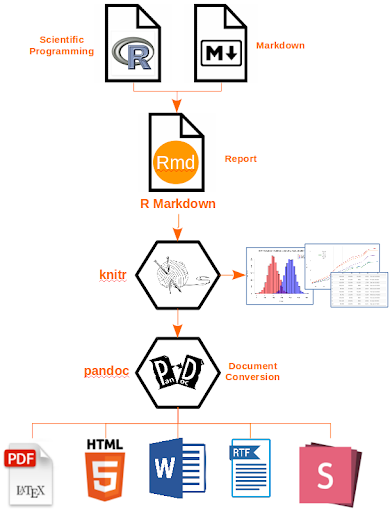
\includegraphics[width=0.6\linewidth]{figures/rmarkdown-flow} 

}

\caption{R Markdown의 최종 결과물 산출과정(http://applied-r.com/project-reporting-template/)}\label{fig:rmarkdown-flow}
\end{figure}

\normalsize

\hypertarget{create-rmd-file}{%
\subsubsection*{R Markdown 문서 시작하기}\label{create-rmd-file}}


\begin{itemize}
\tightlist
\item
  \textbf{R Markdown} 문서 생성: \texttt{{[}File{]}\ -\textgreater{}\ {[}New\ File{]}\ -\textgreater{}\ {[}R\ Markdown..{]}}을 선택
\end{itemize}

\footnotesize

\begin{rmdcaution}
\begin{rmdcaution}

RStudio를 처음 설치하고 위와 같이 진행할 경우 아래와 같은 패키지 설치 여부를 묻는 팝업 창이 나타남. 패키지 설치 여부에 \texttt{{[}Yes{]}}를 클릭하면 R Markdown 문서 생성을 위해 필요한 패키지들이 자동으로 설치

\end{rmdcaution}
\end{rmdcaution}

\normalsize

\footnotesize

\begin{center}\includegraphics[width=0.8\linewidth]{figures/rmarkdown-new-01} \end{center}

\normalsize

\begin{itemize}
\tightlist
\item
  설치 완료 후 R Markdown으로 생성할 최종 문서 유형 선택 질의 창이 나타남. 아래 창에서 제목(Title)과 저자(Author) 이름 입력 후 \texttt{{[}OK{]}} 버튼 클릭(\texttt{Document}, \texttt{html} 문서 선택)
\end{itemize}

\footnotesize

\begin{center}\includegraphics[width=0.8\linewidth]{figures/rmarkdown-new-02} \end{center}

\normalsize

\begin{itemize}
\tightlist
\item
  아래 그림과 같이 새로운 문서 창이 생성되고 \texttt{test.Rmd} 파일로 저장\footnote{\protect\hyperlink{rstudio-project}{RStudio 프로젝트}에서 생성한 폴더 내에 파일 저장}
\end{itemize}

\footnotesize

\begin{center}\includegraphics[width=0.8\linewidth]{figures/rmarkdown-new-03} \end{center}

\normalsize

\begin{itemize}
\tightlist
\item
  문서 상단에 \texttt{Knit} 아이콘을 클릭 후 \texttt{Knit\ to\ HTML} 클릭 또는 문서 아무 곳에 커서를 위치하고 단축키 \texttt{{[}Ctrl{]}\ +\ {[}Shift{]}\ +\ {[}K{]}} 입력
\end{itemize}

\footnotesize

\begin{center}\includegraphics[width=0.8\linewidth]{figures/rmarkdown-new-04} \end{center}

\normalsize

\begin{itemize}
\tightlist
\item
  \texttt{knitr} + \texttt{R\ Markdown} + \texttt{pandoc} \(\rightarrow\) \texttt{html} 파일 생성 결과
\end{itemize}

\footnotesize

\begin{figure}

{\centering \includegraphics[width=0.8\linewidth]{figures/rmarkdown-new-out} 

}

\caption{test.html 문서 화면(저장 폴더 내 `test.html`을 크롬 브라우저로 실행)}\label{fig:rmarkdown-new-out}
\end{figure}

\normalsize

\hypertarget{r-markdown-uxbb38uxc11c-uxad6cuxc131}{%
\subsubsection{R Markdown 문서 구성}\label{r-markdown-uxbb38uxc11c-uxad6cuxc131}}

R Markdown 문서는 아래 그림과 같이 \textbf{YAML}, \textbf{Markdown 텍스트}, \textbf{Code Chunk} 세 부분으로 구성됨.

\footnotesize

\begin{center}\includegraphics[width=0.8\linewidth]{figures/rmarkdown-part} \end{center}

\normalsize

\textbf{1. YAML (YAML Ain't Markup Language)}

\begin{itemize}
\tightlist
\item
  R Markdown 문서의 metadata로 문서의 맨 처음에 항상 포함되어야 함.
\item
  R Markdown 문서의 최종 출력 형태, 제목, 저자, 날짜 등의 정보 등을 포함
\item
  YAML 언어에 대한 사용 예시는 \citet{xie-2016} 의 \href{https://bookdown.org/yihui/bookdown/r-markdown.html}{Appendix B.2} 참고
\item
  최소 형태의 YAML 예시
\end{itemize}

\footnotesize

\begin{Shaded}
\begin{Highlighting}[]
\OtherTok{---}
\FunctionTok{title:}\AttributeTok{ }\StringTok{"Hello R Markdown"}
\FunctionTok{author:}\AttributeTok{ }\StringTok{"Zorba"}
\FunctionTok{date:}\AttributeTok{ }\StringTok{"2020-03-17"}
\FunctionTok{output:}\AttributeTok{ html_document}
\OtherTok{---}
\end{Highlighting}
\end{Shaded}

\normalsize

\textbf{2. Markdown 텍스트}

\begin{itemize}
\tightlist
\item
  Markdown 문법은 15주 차 강의에서 배울 예정임
\item
  \href{https://rstudio.com/wp-content/uploads/2015/03/rmarkdown-reference.pdf}{R Markdown 레퍼런스 가이드} 참조
\item
  그림 삽입: \texttt{!{[}{]}(path/filename)}
\end{itemize}

\begin{Shaded}
\begin{Highlighting}[]
\NormalTok{그립 삽입 구문}
\NormalTok{![](figures/son.jpg)   }
\end{Highlighting}
\end{Shaded}

\includegraphics{figures/son.jpg}

\textbf{3. Code Chunk}

\begin{itemize}
\tightlist
\item
  실제 R code가 실행되는 부분임
\item
  Code chunk 실행 시 다양한 옵션들이 있으나 이 부분 역시 15주 차 강의에서 간략히 다룰 예정임
\item
  Code chunk는 \texttt{\textasciigrave{}\textasciigrave{}\textasciigrave{}\{r\}}로 시작되며 \texttt{r}은 code 언어 이름을 나타냄.
\item
  Code chunk는 \texttt{\textasciigrave{}\textasciigrave{}\textasciigrave{}} 로 종료
\item
  R Markdown 문서 작성 시 단축키 \texttt{{[}Ctrl{]}\ +\ {[}Alt{]}\ +\ {[}I{]}}를 입력하면 Chunk 입력창이 자동 생성됨
\item
  Chunk option에 대한 상세 내용은 \url{https://yihui.org/knitr/options/} 또는 \href{https://rstudio.com/wp-content/uploads/2015/03/rmarkdown-reference.pdf}{R Markdown 레퍼런스 가이드} 참조
\end{itemize}

\begin{Shaded}
\begin{Highlighting}[]
\NormalTok{Code chunk 예시}

\NormalTok{Xie의 R Markdown: The Definitive Guide에서 발췌}

\BaseNTok{```\{r\}}
\BaseNTok{fit = lm(dist ~ speed, data = cars)}
\BaseNTok{b   = coef(fit)}
\BaseNTok{plot(cars)}
\BaseNTok{abline(fit)}
\BaseNTok{```}
\end{Highlighting}
\end{Shaded}

\footnotesize

\begin{Shaded}
\begin{Highlighting}[]
\NormalTok{fit =}\StringTok{ }\KeywordTok{lm}\NormalTok{(dist }\OperatorTok{~}\StringTok{ }\NormalTok{speed, }\DataTypeTok{data =}\NormalTok{ cars)}
\NormalTok{b   =}\StringTok{ }\KeywordTok{coef}\NormalTok{(fit)}
\KeywordTok{plot}\NormalTok{(cars)}
\KeywordTok{abline}\NormalTok{(fit)}
\end{Highlighting}
\end{Shaded}

\includegraphics{01-overview_files/figure-latex/unnamed-chunk-44-1.pdf}

\normalsize

\begin{itemize}
\tightlist
\item
  Code chunk에서 외부 그림 파일 불러오기(\citet{xie-2018} 에서 예시 발췌)
\end{itemize}

\footnotesize

\begin{Shaded}
\begin{Highlighting}[]
\NormalTok{knitr}\OperatorTok{::}\KeywordTok{include_graphics}\NormalTok{(}\KeywordTok{rep}\NormalTok{(}\StringTok{'figures/knit-logo.png'}\NormalTok{, }\DecValTok{3}\NormalTok{))}
\end{Highlighting}
\end{Shaded}

\includegraphics[width=0.328\linewidth]{figures/knit-logo} \includegraphics[width=0.328\linewidth]{figures/knit-logo} \includegraphics[width=0.328\linewidth]{figures/knit-logo}

\normalsize

\footnotesize

\begin{rmdimportant}
\begin{rmdimportant}

\textbf{Homework 1}: R Markdown 문서에 아래 내용을 포함한 문서를 \texttt{html} 파일 형식으로 출력 후 제출

\begin{itemize}
\tightlist
\item
  간략한 자기소개 및 ``통계 프로그래밍 언어'' 수업에 대한 본인만의 목표 기술
\item
  본인이 setting 한 RStudio 구성 캡쳐 화면을 그림 파일로 저장하고 R Markdown 문서에 삽입(화면 캡쳐 시 생성 프로젝트 내 폴더 내용 반드시 포함)
\item
  패키지 \texttt{ggplot2}를 불러오고 \texttt{cars} 데이터셋의 2차원 산점도(\textbf{hint}: \texttt{help(geom\_point)} 또는 googling 활용)를 문서에 포함
\end{itemize}

\end{rmdimportant}
\end{rmdimportant}

\normalsize

\hypertarget{data-type}{%
\chapter{R 객체(R object)}\label{data-type}}

\footnotesize

\begin{rmdnote}
\begin{rmdnote}

\textbf{학습목표(2 주차)}: R에서 사용 가능한 데이터 타입에 대해 알아보고, 고유 데이터 타입으로 구성한 객체(스칼라, 백터, 리스트)와 이와 연관된 함수들을 익힌다.

\end{rmdnote}
\end{rmdnote}

\normalsize

\hypertarget{ch2-abstract}{%
\subsubsection*{학습 필요성}\label{ch2-abstract}}


\begin{itemize}
\tightlist
\item
  R언어는 타 프로그래밍 언어와 유사한 데이터 타입(정수형, 실수형, 문자형 등)을 제공
\item
  R 언어가 다른 언어와 차이점 \(\rightarrow\) \textbf{데이터 분석}에 특화된 벡터(vector), 행렬(matrix), 데이터프레임(data frame), 리스트(list)와 같은 객체\footnote{R에서 사용자가 데이터 입력을 위해 생성 또는 읽어온 객체(object)는 종종 변수(variable)라는 말과 혼용. 본 문서에서는 최상위 데이터 저장장소를 객체라고 명명하며 데이터프레임과 같이 여러 종류의 데이터타입으로 이루어진 객체의 1차원 속성을 변수라고 칭함} 제공
\item
  R 패키지에서 제공되는 함수 사용 방법은 R의 객체에 따라 달라질 수 있음\\
\item
  R 언어를 원활히 다룰 수 있으려면 R에서 데이터 객체의 형태, 자료 할당 및 그 연산 방법에 대한 이해가 필수적으로 선행되어야 함
\end{itemize}

\hypertarget{object-value}{%
\subsubsection*{R의 데이터 타입}\label{object-value}}


\begin{itemize}
\item
  \textbf{수치형(numeric)}: 숫자(정수, 소수)
\item
  \textbf{문자열(string)}: \texttt{"충남대학교"}, \texttt{"R강의"}
\item
  \textbf{논리형(logical)}: \texttt{TRUE}/\texttt{FALSE}
\item
  \textbf{결측값(\texttt{NA})}: 자료에서 발생한 결측 표현
\item
  \textbf{공백(\texttt{NULL})}: 지정하지 않은 값
\item
  \textbf{요인(factor)}: 범주형 자료 표현(수치 + 문자 결합 형태로 이해하면 편함)
\item
  \textbf{기타}: 숫자아님(\texttt{NaN}), 무한대(\texttt{Inf}) 등
\end{itemize}

\hypertarget{ch2-object-type}{%
\subsubsection*{R 객체의 종류}\label{ch2-object-type}}


\begin{itemize}
\tightlist
\item
  스칼라(상수형, scalar 또는 atomic)
\item
  벡터(vector): \textbf{R의 기본연산 단위}
\item
  리스트(list)
\item
  행렬(matrix)
\item
  배열(array)
\item
  데이터프레임(data frame)
\end{itemize}

\textbf{아래 그림은 2\textasciitilde4 주차에 배울 R 주요 객체에 대한 개요도임}

\footnotesize

\begin{figure}

{\centering \includegraphics[width=1\linewidth]{figures/datatype-diagram} 

}

\caption{R 데이터 타입 구조 다이어그램: [R, Python 분석과 프로그래밍 (by R Friend)]( http://rfriend.tistory.com/)에서 발췌 후 수정}\label{fig:rmarkdown-part}
\end{figure}

\normalsize

\hypertarget{scalar}{%
\section{스칼라(scalar)}\label{scalar}}

\begin{itemize}
\tightlist
\item
  단일 차원의 값(하나의 값): \(1 \times 1\) 백터로 표현 \(\rightarrow\) R 데이터 객체의 기본은 벡터!!
\item
  데이터 객체의 유형은 크게 숫자형, 문자열, 논리형이 있음
\end{itemize}

\footnotesize

\begin{rmdtip}
\begin{rmdtip}

스칼라를 입력시 R의 벡터 지정 함수인 \texttt{c()}(벡터 부분에서 상세 내용 학습)를 꼭 사용해서 입력할 필요가 없다. 단, 연속되지 않은 두 개 이상 스칼라면 벡터이므로 꼭 c()를 써야 한다.

\end{rmdtip}
\end{rmdtip}

\normalsize

\hypertarget{definition}{%
\subsection{선언}\label{definition}}

\begin{itemize}
\tightlist
\item
  일반적으로 컴파일이 필요한 언어(예: \texttt{C} 언어)의 경우 변수 또는 객체를 사용 전에 선언이 필요
\end{itemize}

\footnotesize

\begin{Shaded}
\begin{Highlighting}[]
\DataTypeTok{int}\NormalTok{ x; }
\NormalTok{x = }\DecValTok{1}\NormalTok{;}
\end{Highlighting}
\end{Shaded}

\normalsize

\begin{itemize}
\item
  위 코드에서 \texttt{int\ x;} 없이 \texttt{x\ =\ 1}을 입력 후 컴파일 하면 에러가 나타나지만 \texttt{R} 언어에서는 \textbf{변수를 선언할 필요가 전혀 없음}
\item
  \texttt{z} 가 어떤 데이터 타입인지 언급할 필요가 전혀 없음 \(\rightarrow\) \texttt{Python}, \texttt{Perl}, \texttt{Matlab} 등과 같은 스크립트 언어의 특징. 아래 코드 참조
\end{itemize}

\footnotesize

\begin{Shaded}
\begin{Highlighting}[]
\NormalTok{z <-}\StringTok{ }\DecValTok{3}
\NormalTok{z}
\end{Highlighting}
\end{Shaded}

\begin{verbatim}
[1] 3
\end{verbatim}

\normalsize

\hypertarget{numeric}{%
\subsection{숫자형}\label{numeric}}

\begin{itemize}
\tightlist
\item
  정수형(integer)과 실수형(double)로 구분됨
\item
  정수형 구분시 숫자 뒤 \texttt{L}을 표시
\end{itemize}

\footnotesize

\begin{Shaded}
\begin{Highlighting}[]
\CommentTok{# 정수형 구분자 사용 예시}
\CommentTok{# typeof(): R 객체의 데이터 타입 반환하는 함수}
\KeywordTok{typeof}\NormalTok{(10L)}
\end{Highlighting}
\end{Shaded}

\begin{verbatim}
[1] "integer"
\end{verbatim}

\begin{Shaded}
\begin{Highlighting}[]
\KeywordTok{typeof}\NormalTok{(}\DecValTok{10}\NormalTok{)}
\end{Highlighting}
\end{Shaded}

\begin{verbatim}
[1] "double"
\end{verbatim}

\normalsize

\begin{itemize}
\tightlist
\item
  수치연산(\texttt{+,\ -,\ *,\ \^{},\ **,\ /,\ \%\%,\ \%/\%}) 가능: R은 함수형 언어이기 때문에 앞에 기술한 연산자도 하나의 함수로 인식함.
\item
  수치 연산자(operator) 및 기본 수학 함수
\end{itemize}

\footnotesize

\begin{table}[H]

\caption{\label{tab:operation}R언어의 기본 수치 연산자}
\centering
\fontsize{10}{12}\selectfont
\begin{tabular}[t]{>{\raggedright\arraybackslash}p{4cm}>{\raggedright\arraybackslash}p{6cm}}
\toprule
수치형 연산자 & 설명\\
\midrule
\rowcolor{gray!6}  \ttfamily{+, -, *, /} & \ttfamily{사칙연산}\\
\ttfamily{n \%\% m} & \ttfamily{n을 m 으로 나눈 나머지}\\
\rowcolor{gray!6}  \ttfamily{n \%/\% m} & \ttfamily{n을 m 으로 나눈 몫}\\
\ttfamily{n \textasciicircum{} m 또는 n ** m} & \ttfamily{n 의 m 승}\\
\bottomrule
\end{tabular}
\end{table}

\normalsize

\textbf{숫자형 스칼라 연산 적용 예시}

\footnotesize

\begin{Shaded}
\begin{Highlighting}[]
\CommentTok{# 숫자형 스칼라}
\NormalTok{a <-}\StringTok{ }\DecValTok{3}
\NormalTok{b <-}\StringTok{ }\DecValTok{10}
\NormalTok{a; b}
\end{Highlighting}
\end{Shaded}

\begin{verbatim}
[1] 3
\end{verbatim}

\begin{verbatim}
[1] 10
\end{verbatim}

\begin{Shaded}
\begin{Highlighting}[]
\CommentTok{# 덧셈}
\NormalTok{c <-}\StringTok{ }\NormalTok{a }\OperatorTok{+}\StringTok{ }\NormalTok{b}
\NormalTok{c}
\end{Highlighting}
\end{Shaded}

\begin{verbatim}
[1] 13
\end{verbatim}

\begin{Shaded}
\begin{Highlighting}[]
\CommentTok{# 덧셈을 함수로 입력}
\CommentTok{# "+"(a, b)로 입력한 결과}
\NormalTok{c <-}\StringTok{ "+"}\NormalTok{(a, b)}

\CommentTok{# 뺄셈}
\NormalTok{d <-}\StringTok{ }\NormalTok{b }\OperatorTok{-}\StringTok{ }\NormalTok{a}
\NormalTok{d}
\end{Highlighting}
\end{Shaded}

\begin{verbatim}
[1] 7
\end{verbatim}

\begin{Shaded}
\begin{Highlighting}[]
\CommentTok{# 곱셈}
\NormalTok{m <-}\StringTok{ }\NormalTok{a }\OperatorTok{*}\StringTok{ }\NormalTok{b}
\NormalTok{m}
\end{Highlighting}
\end{Shaded}

\begin{verbatim}
[1] 30
\end{verbatim}

\begin{Shaded}
\begin{Highlighting}[]
\CommentTok{# 나누기}
\NormalTok{dd <-}\StringTok{ }\NormalTok{b}\OperatorTok{/}\NormalTok{a}
\NormalTok{dd}
\end{Highlighting}
\end{Shaded}

\begin{verbatim}
[1] 3.333333
\end{verbatim}

\begin{Shaded}
\begin{Highlighting}[]
\CommentTok{# 멱승}
\NormalTok{b}\OperatorTok{^}\NormalTok{a}
\end{Highlighting}
\end{Shaded}

\begin{verbatim}
[1] 1000
\end{verbatim}

\begin{Shaded}
\begin{Highlighting}[]
\CommentTok{# 나누기의 나머지(remainder) 반환}
\NormalTok{r <-}\StringTok{ }\NormalTok{b }\OperatorTok\StringTok{ }\NormalTok{a}
\NormalTok{r}
\end{Highlighting}
\end{Shaded}

\begin{verbatim}
[1] 1
\end{verbatim}

\begin{Shaded}
\begin{Highlighting}[]
\CommentTok{# 나누기의 몫(quotient) 반환}
\NormalTok{q <-}\StringTok{ }\NormalTok{b }\OperatorTok\StringTok{ }\NormalTok{a}
\NormalTok{q}
\end{Highlighting}
\end{Shaded}

\begin{verbatim}
[1] 3
\end{verbatim}

\begin{Shaded}
\begin{Highlighting}[]
\CommentTok{# 연산 우선 순위}
\NormalTok{nn <-}\StringTok{ }\NormalTok{(}\DecValTok{3} \OperatorTok{+}\StringTok{ }\DecValTok{5}\NormalTok{)}\OperatorTok{*}\DecValTok{3} \OperatorTok{-}\StringTok{ }\DecValTok{4}\OperatorTok{**}\DecValTok{2}\OperatorTok{/}\DecValTok{4}
\NormalTok{nn}
\end{Highlighting}
\end{Shaded}

\begin{verbatim}
[1] 20
\end{verbatim}

\normalsize

\hypertarget{character}{%
\subsection{문자형}\label{character}}

\begin{itemize}
\tightlist
\item
  수치형이 아닌 문자 형식의 단일 원소
\item
  C와 같은 언어에서 볼수 있는 한개 문자에 대한 데이터 타입 존재하지 않음
\item
  수치연산 불가능
\item
  따옴표(\texttt{"} 또는 \texttt{\textquotesingle{}})로 문자를 묶어서 문자열 표시
\item
  문자열을 다루는 자세한 설명은 5주차에서 자세히 설명할 예정임
\end{itemize}

\footnotesize

\begin{Shaded}
\begin{Highlighting}[]
\NormalTok{h1 <-}\StringTok{ }\KeywordTok{c}\NormalTok{(}\StringTok{"Hello CNU!!"}\NormalTok{)}
\NormalTok{h2 <-}\StringTok{ }\KeywordTok{c}\NormalTok{(}\StringTok{"R is not too difficult."}\NormalTok{)}
\KeywordTok{typeof}\NormalTok{(h1); }\KeywordTok{typeof}\NormalTok{(h2)}
\end{Highlighting}
\end{Shaded}

\begin{verbatim}
[1] "character"
\end{verbatim}

\begin{verbatim}
[1] "character"
\end{verbatim}

\begin{Shaded}
\begin{Highlighting}[]
\NormalTok{h1}
\end{Highlighting}
\end{Shaded}

\begin{verbatim}
[1] "Hello CNU!!"
\end{verbatim}

\begin{Shaded}
\begin{Highlighting}[]
\NormalTok{h2}
\end{Highlighting}
\end{Shaded}

\begin{verbatim}
[1] "R is not too difficult."
\end{verbatim}

\begin{Shaded}
\begin{Highlighting}[]
\CommentTok{# 문자열의 문자 수 반환}
\KeywordTok{nchar}\NormalTok{(h1); }\KeywordTok{nchar}\NormalTok{(h2)}
\end{Highlighting}
\end{Shaded}

\begin{verbatim}
[1] 11
\end{verbatim}

\begin{verbatim}
[1] 23
\end{verbatim}

\begin{Shaded}
\begin{Highlighting}[]
\CommentTok{# 문자열 연산 error 예시}
\NormalTok{h1 }\OperatorTok{-}\StringTok{ }\NormalTok{h2}
\end{Highlighting}
\end{Shaded}

\begin{verbatim}
Error in h1 - h2: 이항연산자에 수치가 아닌 인수입니다
\end{verbatim}

\normalsize

\hypertarget{logical}{%
\subsection{논리형 스칼라}\label{logical}}

\begin{itemize}
\tightlist
\item
  참(\texttt{TRUE}, \texttt{T}) 또는 거짓(\texttt{FALSE}, \texttt{F})를 나타내는 값
\item
  \texttt{TRUE}/\texttt{FALSE}: 예약어(reserved word)
\item
  \texttt{T}/\texttt{F}: \texttt{TRUE}와 \texttt{FALSE}로 초기화된 전역 변수

  \begin{itemize}
  \tightlist
  \item
    \texttt{T}에 \texttt{FALSE} 또는 어떤 값도 할당 가능 \(\rightarrow\) 가급적 \texttt{TRUE/FALSE}를 명시하는 것이 편함
  \end{itemize}
\item
  논리형 연산자(logical operator)
\end{itemize}

\footnotesize

\begin{table}[H]

\caption{\label{tab:logic-op-tab}R언어의 논리형 연산자}
\centering
\fontsize{10}{12}\selectfont
\begin{tabular}[t]{>{\raggedright\arraybackslash}p{3cm}>{\raggedright\arraybackslash}p{7cm}}
\toprule
논리형 연산자 & 설명\\
\midrule
\rowcolor{gray!6}  \ttfamily{\&} & \ttfamily{AND (vectorized)}\\
\ttfamily{\&\&} & \ttfamily{AND (atomic)}\\
\rowcolor{gray!6}  \ttfamily{|} & \ttfamily{OR (vectorized)}\\
\ttfamily{||} & \ttfamily{OR (atomic)}\\
\rowcolor{gray!6}  \ttfamily{!} & \ttfamily{NOT}\\
\bottomrule
\end{tabular}
\end{table}

\normalsize

\begin{itemize}
\tightlist
\item
  비교 연산자를 적용할 경우 논리값을 반환
\end{itemize}

\footnotesize

\begin{table}[H]

\caption{\label{tab:comp-op-tab}R언어의 비교 연산자}
\centering
\fontsize{10}{12}\selectfont
\begin{threeparttable}
\begin{tabular}[t]{>{\raggedright\arraybackslash}p{3cm}>{\raggedright\arraybackslash}p{7cm}}
\toprule
비교 연산자 & 설명\\
\midrule
\rowcolor{gray!6}  \ttfamily{>} & \ttfamily{크다(greater-than)}\\
\ttfamily{<} & \ttfamily{작다(less-than)}\\
\rowcolor{gray!6}  \ttfamily{==} & \ttfamily{같다(equal)}\\
\ttfamily{>=} & \ttfamily{크거나 같다(greater than equal)}\\
\rowcolor{gray!6}  \ttfamily{<=} & \ttfamily{작거나 같다(less than equal)}\\
\addlinespace
\ttfamily{!=} & \ttfamily{같지 않다(not equal)}\\
\bottomrule
\end{tabular}
\begin{tablenotes}
\item \textit{Note: } 
\item 기술한 비교 연산자는 수치형 및 논리형 데이터 타입 모두에 적용 가능 하지만, 문자형은 비교 연산은 ==, != 만 가능함
\end{tablenotes}
\end{threeparttable}
\end{table}

\normalsize

\footnotesize

\begin{rmdnote}
\begin{rmdnote}

\textbf{참고}

\begin{itemize}
\tightlist
\item
  논리형 스칼라도 숫자형 연산 가능 \(\rightarrow\) 컴퓨터는 \texttt{TRUE}/\texttt{FALSE}를 1과 0 숫자로 인식
\item
  수치 연산자는 스칼라 뿐 아니라 아래에서 다룰 벡터, 행렬, 리스트, 데이터프레임 객체의 연산에 사용 가능
\item
  \texttt{\&}/\texttt{\textbar{}}와 \texttt{\&\&}/\texttt{\textbar{}\textbar{}}는 동일하게 AND/OR를 의미하지만 연산 결과가 다름.
\item
  \texttt{\&}의 연산 대상이 벡터인 경우 백터 구성 값 각각에 대해 \texttt{\&} 연산을 실행 하지만 \texttt{\&\&}는 하나의 값(스칼라)에만 논리 연산이 적용(아래 예시 참고)
\end{itemize}

\end{rmdnote}
\end{rmdnote}

\normalsize

\begin{itemize}
\tightlist
\item
  논리형 스칼라의 논리 및 비교 연산 예시
\end{itemize}

\footnotesize

\begin{Shaded}
\begin{Highlighting}[]
\KeywordTok{typeof}\NormalTok{(}\OtherTok{TRUE}\NormalTok{)  }\CommentTok{# TRUE의 데이터 타입}
\end{Highlighting}
\end{Shaded}

\begin{verbatim}
[1] "logical"
\end{verbatim}

\begin{Shaded}
\begin{Highlighting}[]
\OtherTok{TRUE} \OperatorTok{&}\StringTok{ }\OtherTok{TRUE}  \CommentTok{# TRUE 반환}
\end{Highlighting}
\end{Shaded}

\begin{verbatim}
[1] TRUE
\end{verbatim}

\begin{Shaded}
\begin{Highlighting}[]
\OtherTok{TRUE} \OperatorTok{&}\StringTok{ }\OtherTok{FALSE}  \CommentTok{# FALSE 반환}
\end{Highlighting}
\end{Shaded}

\begin{verbatim}
[1] FALSE
\end{verbatim}

\begin{Shaded}
\begin{Highlighting}[]
\CommentTok{# 아래 연산은 모두 TRUE 반환}
\OtherTok{TRUE} \OperatorTok{|}\StringTok{ }\OtherTok{TRUE}
\end{Highlighting}
\end{Shaded}

\begin{verbatim}
[1] TRUE
\end{verbatim}

\begin{Shaded}
\begin{Highlighting}[]
\OtherTok{TRUE} \OperatorTok{|}\StringTok{ }\OtherTok{FALSE}
\end{Highlighting}
\end{Shaded}

\begin{verbatim}
[1] TRUE
\end{verbatim}

\begin{Shaded}
\begin{Highlighting}[]
\CommentTok{# TRUE와 FALSE의 반대}
\OperatorTok{!}\OtherTok{TRUE}
\end{Highlighting}
\end{Shaded}

\begin{verbatim}
[1] FALSE
\end{verbatim}

\begin{Shaded}
\begin{Highlighting}[]
\OperatorTok{!}\OtherTok{FALSE}
\end{Highlighting}
\end{Shaded}

\begin{verbatim}
[1] TRUE
\end{verbatim}

\begin{Shaded}
\begin{Highlighting}[]
\CommentTok{# 전역변수 T에 FALSE 값 할당}
\NormalTok{T <-}\StringTok{ }\OtherTok{FALSE}
\NormalTok{T}
\end{Highlighting}
\end{Shaded}

\begin{verbatim}
[1] FALSE
\end{verbatim}

\begin{Shaded}
\begin{Highlighting}[]
\NormalTok{T <-}\StringTok{ }\OtherTok{TRUE}  \CommentTok{# 원상복귀}
\CommentTok{# TRUE/FALSE에 값을 할당할 수 없음}
\OtherTok{TRUE}\NormalTok{ <-}\StringTok{ }\DecValTok{1}
\end{Highlighting}
\end{Shaded}

\begin{verbatim}
Error in TRUE <- 1: 대입에 유효하지 않은 (do_set) 좌변입니다
\end{verbatim}

\begin{Shaded}
\begin{Highlighting}[]
\OtherTok{TRUE}\NormalTok{ <-}\StringTok{ }\OtherTok{FALSE}
\end{Highlighting}
\end{Shaded}

\begin{verbatim}
Error in TRUE <- FALSE: 대입에 유효하지 않은 (do_set) 좌변입니다
\end{verbatim}

\begin{Shaded}
\begin{Highlighting}[]
\CommentTok{# &(|)와 &&(||)의 차이}
\NormalTok{l}\FloatTok{.01}\NormalTok{ <-}\StringTok{ }\KeywordTok{c}\NormalTok{(}\OtherTok{TRUE}\NormalTok{, }\OtherTok{TRUE}\NormalTok{, }\OtherTok{FALSE}\NormalTok{, }\OtherTok{TRUE}\NormalTok{)  }\CommentTok{# 논리형 값으로 구성된 벡터}
\NormalTok{l}\FloatTok{.02}\NormalTok{ <-}\StringTok{ }\KeywordTok{c}\NormalTok{(}\OtherTok{FALSE}\NormalTok{, }\OtherTok{TRUE}\NormalTok{, }\OtherTok{TRUE}\NormalTok{, }\OtherTok{TRUE}\NormalTok{)}
\NormalTok{l}\FloatTok{.01} \OperatorTok{&}\StringTok{ }\NormalTok{l}\FloatTok{.02}  \CommentTok{# l.01과 l.02 각 원소 별 & 연산}
\end{Highlighting}
\end{Shaded}

\begin{verbatim}
[1] FALSE  TRUE FALSE  TRUE
\end{verbatim}

\begin{Shaded}
\begin{Highlighting}[]
\NormalTok{l}\FloatTok{.01} \OperatorTok{&&}\StringTok{ }\NormalTok{l}\FloatTok{.02}  \CommentTok{# l.01과 l.02의 첫 번째 원소에 대해 & 연산}
\end{Highlighting}
\end{Shaded}

\begin{verbatim}
[1] FALSE
\end{verbatim}

\begin{Shaded}
\begin{Highlighting}[]
\CommentTok{# 비교 연산자}
\NormalTok{x <-}\StringTok{ }\DecValTok{9}
\NormalTok{y <-}\StringTok{ }\DecValTok{4}
\CommentTok{# x > y 의 반환값 데이터 타입}
\KeywordTok{typeof}\NormalTok{(x }\OperatorTok{>}\StringTok{ }\NormalTok{y)}
\end{Highlighting}
\end{Shaded}

\begin{verbatim}
[1] "logical"
\end{verbatim}

\begin{Shaded}
\begin{Highlighting}[]
\CommentTok{# 논리형 값 반환}
\NormalTok{x }\OperatorTok{>}\StringTok{ }\NormalTok{y}
\end{Highlighting}
\end{Shaded}

\begin{verbatim}
[1] TRUE
\end{verbatim}

\begin{Shaded}
\begin{Highlighting}[]
\NormalTok{x }\OperatorTok{<}\StringTok{ }\NormalTok{y}
\end{Highlighting}
\end{Shaded}

\begin{verbatim}
[1] FALSE
\end{verbatim}

\begin{Shaded}
\begin{Highlighting}[]
\NormalTok{x }\OperatorTok{==}\StringTok{ }\NormalTok{y}
\end{Highlighting}
\end{Shaded}

\begin{verbatim}
[1] FALSE
\end{verbatim}

\begin{Shaded}
\begin{Highlighting}[]
\NormalTok{x }\OperatorTok{!=}\StringTok{ }\NormalTok{y}
\end{Highlighting}
\end{Shaded}

\begin{verbatim}
[1] TRUE
\end{verbatim}

\normalsize

\hypertarget{missing-value}{%
\subsection{결측값(missing value)}\label{missing-value}}

\begin{itemize}
\tightlist
\item
  결측치 지정 \textbf{상수}: \texttt{NA} \(\rightarrow\) R과 다른 언어의 가장 큰 차이점 중 하나
\item
  예를 들어 4명의 통계학과 학생 중 3명의 통계학 개론 중간고사 점수가 각각 80, 90, 75점이고 4번 째 학생의 점수가 없는 경우 \texttt{NA}로 결측값 표현
\item
  \texttt{is.na()} 함수를 이용해 해당 값이 결측을 포함하고 있는지 확인
\end{itemize}

\footnotesize

\begin{Shaded}
\begin{Highlighting}[]
\NormalTok{one <-}\StringTok{ }\DecValTok{80}\NormalTok{; two <-}\StringTok{ }\DecValTok{90}\NormalTok{; three <-}\StringTok{ }\DecValTok{75}\NormalTok{; four <-}\StringTok{ }\OtherTok{NA}
\NormalTok{four}
\end{Highlighting}
\end{Shaded}

\begin{verbatim}
[1] NA
\end{verbatim}

\begin{Shaded}
\begin{Highlighting}[]
\CommentTok{# 'is.na()' 결측 NA가 포함되어 있으면 TRUE }
\KeywordTok{is.na}\NormalTok{(four)}
\end{Highlighting}
\end{Shaded}

\begin{verbatim}
[1] TRUE
\end{verbatim}

\normalsize

\footnotesize

\begin{rmdtip}
\begin{rmdtip}

\texttt{is.na(object\_name)}: 객체를 구성하고 있는 원소 중 \texttt{NA}를 포함하고 있는지 확인 \(\rightarrow\) \texttt{NA}를 포함하면 \texttt{TRUE}, 아니면 \texttt{FALSE} 반환

\textbf{참고}: 자료에 \texttt{NA}가 포함된 경우 연산 결과는 모두 \texttt{NA}가 반환

\end{rmdtip}
\end{rmdtip}

\normalsize

\footnotesize

\begin{Shaded}
\begin{Highlighting}[]
\OtherTok{NA} \OperatorTok{+}\StringTok{ }\DecValTok{1}
\end{Highlighting}
\end{Shaded}

\begin{verbatim}
[1] NA
\end{verbatim}

\begin{Shaded}
\begin{Highlighting}[]
\OtherTok{NA} \OperatorTok{&}\StringTok{ }\OtherTok{TRUE}
\end{Highlighting}
\end{Shaded}

\begin{verbatim}
[1] NA
\end{verbatim}

\begin{Shaded}
\begin{Highlighting}[]
\OtherTok{NA} \OperatorTok{<=}\StringTok{ }\DecValTok{3}
\end{Highlighting}
\end{Shaded}

\begin{verbatim}
[1] NA
\end{verbatim}

\normalsize

\hypertarget{null}{%
\subsection{NULL 값}\label{null}}

\begin{itemize}
\tightlist
\item
  \texttt{NULL}: 초기화 되지 않은 변수 또는 \textbf{객체}를 지칭함
\item
  \texttt{is.null()} 함수를 통해 객체가 \texttt{NULL}인지 판단
\end{itemize}

\footnotesize

\begin{Shaded}
\begin{Highlighting}[]
\NormalTok{x <-}\StringTok{ }\OtherTok{NULL} \CommentTok{# NULL 지정}
\KeywordTok{is.null}\NormalTok{(x) }\CommentTok{# NULL 객체인지 판단}
\end{Highlighting}
\end{Shaded}

\begin{verbatim}
[1] TRUE
\end{verbatim}

\begin{Shaded}
\begin{Highlighting}[]
\NormalTok{x <-}\StringTok{ }\DecValTok{1}
\KeywordTok{is.null}\NormalTok{(x) }
\end{Highlighting}
\end{Shaded}

\begin{verbatim}
[1] FALSE
\end{verbatim}

\normalsize

\footnotesize

\begin{rmdnote}
\begin{rmdnote}

\textbf{\texttt{NA}와 \texttt{NULL}의 차이점}: 자료의 공백을 의미한다는 점에서 유사한 측면이 있으나 아래 내용처럼 큰 차이가 있음

\begin{itemize}
\tightlist
\item
  \texttt{NULL}: 값을 지정하지 않은 객체를 표현하는데 사용. 즉 아직 변수 또는 객체의 상태가 아직 미정인 상태를 나타냄
\item
  \texttt{NA}: 데이터 값이 결측임을 지정해주는 논리형 상수
\end{itemize}

\end{rmdnote}
\end{rmdnote}

\normalsize

\footnotesize

\begin{Shaded}
\begin{Highlighting}[]
\CommentTok{# NA와 NULL은 다름}
\NormalTok{x <-}\StringTok{ }\OtherTok{NA}
\KeywordTok{is.null}\NormalTok{(}\OtherTok{NA}\NormalTok{)}
\end{Highlighting}
\end{Shaded}

\begin{verbatim}
[1] FALSE
\end{verbatim}

\begin{Shaded}
\begin{Highlighting}[]
\KeywordTok{is.na}\NormalTok{(}\OtherTok{NULL}\NormalTok{)}
\end{Highlighting}
\end{Shaded}

\begin{verbatim}
logical(0)
\end{verbatim}

\normalsize

\hypertarget{finite}{%
\subsection{무한대/무한소/숫자아님}\label{finite}}

\begin{itemize}
\tightlist
\item
  \texttt{Inf}: 무한대(\(+\infty\), \(1/0\))
\item
  \texttt{-Inf}: 무한소(\(-\infty\), \(-1/0\))
\item
  \texttt{NaN}: 숫자아님(Not a Number, \(0/0\))
\item
  \texttt{is.finite()}, \texttt{is.infinite()}, \texttt{is.nan()} 함수를 통해 객체가 \texttt{Inf} 또는 \texttt{NaN}을 포함하는지 확인
\end{itemize}

\footnotesize

\begin{Shaded}
\begin{Highlighting}[]
\NormalTok{x <-}\StringTok{ }\OtherTok{Inf}
\KeywordTok{is.finite}\NormalTok{(x)}
\end{Highlighting}
\end{Shaded}

\begin{verbatim}
[1] FALSE
\end{verbatim}

\begin{Shaded}
\begin{Highlighting}[]
\KeywordTok{is.infinite}\NormalTok{(x)}
\end{Highlighting}
\end{Shaded}

\begin{verbatim}
[1] TRUE
\end{verbatim}

\begin{Shaded}
\begin{Highlighting}[]
\NormalTok{x <-}\StringTok{ }\DecValTok{0}\OperatorTok{/}\DecValTok{0}
\KeywordTok{is.nan}\NormalTok{(x)}
\end{Highlighting}
\end{Shaded}

\begin{verbatim}
[1] TRUE
\end{verbatim}

\begin{Shaded}
\begin{Highlighting}[]
\KeywordTok{is.infinite}\NormalTok{(x)}
\end{Highlighting}
\end{Shaded}

\begin{verbatim}
[1] FALSE
\end{verbatim}

\normalsize

\footnotesize

\begin{rmdnote}
\begin{rmdnote}

지금까지 요인형(factor)을 제외하고 R 언어에서 객체가 가질 수 있는 데이터 유형에 대해 알아봄. 요인형은 4주 차에 예정된 ``R 자료형: 팩터, 테이블, 데이터 프레임''에서 상세하게 배울 예정임.

\end{rmdnote}
\end{rmdnote}

\normalsize

\hypertarget{vector}{%
\section{벡터(vector)}\label{vector}}

\hypertarget{vector-prop}{%
\subsection{벡터의 특징}\label{vector-prop}}

\begin{itemize}
\tightlist
\item
  타 프로그래밍 언어의 배열(array)의 개념으로 \textbf{동일한 유형}의 데이터 원소가 하나 이상(\(n \times 1\), \(n \geq 1\)) 으로 구성된 자료 형태
\item
  R 언어의 가장 기본적인 데이터 형태로 R에서 행해지는 모든 연산의 기본(vectorization) \(\rightarrow\) 벡터 연산 시 반복구문(예: \texttt{for\ loop})이 필요 없음.
\item
  \ref{scalar} 절에서 기술한 \protect\hyperlink{scalar}{스칼라(scalar)}는 사실 \(1 \times 1\) 벡터임
\item
  수학적으로 벡터는 아래와 같이 나타낼 수 있음
\end{itemize}

\[\mathrm{\mathbf x} = [x_1, x_2, x_3, \ldots, x_n]^T
\]

\begin{itemize}
\tightlist
\item
  벡터는 앞의 예시에서 본 바와 같이 \texttt{c()} 함수를 사용해 생성
\end{itemize}

\footnotesize

\begin{Shaded}
\begin{Highlighting}[]
\CommentTok{# 숫자형 벡터 }
\NormalTok{x <-}\StringTok{ }\KeywordTok{c}\NormalTok{(}\DecValTok{2}\NormalTok{, }\DecValTok{0}\NormalTok{, }\DecValTok{2}\NormalTok{, }\DecValTok{0}\NormalTok{, }\DecValTok{0}\NormalTok{, }\DecValTok{3}\NormalTok{, }\DecValTok{2}\NormalTok{, }\DecValTok{4}\NormalTok{)}
\NormalTok{x}
\end{Highlighting}
\end{Shaded}

\begin{verbatim}
[1] 2 0 2 0 0 3 2 4
\end{verbatim}

\begin{Shaded}
\begin{Highlighting}[]
\CommentTok{# 문자형 벡터}
\NormalTok{y <-}\StringTok{ }\KeywordTok{c}\NormalTok{(}\StringTok{"Boncho Ku"}\NormalTok{, }\StringTok{"R programming"}\NormalTok{, }\StringTok{"Male"}\NormalTok{, }\StringTok{"sophomore"}\NormalTok{, }\StringTok{"2020-03-24"}\NormalTok{)}
\NormalTok{y}
\end{Highlighting}
\end{Shaded}

\begin{verbatim}
[1] "Boncho Ku"     "R programming" "Male"          "sophomore"    
[5] "2020-03-24"   
\end{verbatim}

\normalsize

\begin{itemize}
\tightlist
\item
  두 개 이상의 벡터는 \texttt{c()} 함수를 통해 결합 가능

  \begin{itemize}
  \tightlist
  \item
    함수 내 \texttt{,} 구분자를 통해 결합
  \end{itemize}
\end{itemize}

\footnotesize

\begin{Shaded}
\begin{Highlighting}[]
\CommentTok{# 두 벡터의 결합 (1)}
\NormalTok{x <-}\StringTok{ }\DecValTok{1}\OperatorTok{:}\DecValTok{5}
\NormalTok{y <-}\StringTok{ }\DecValTok{10}\OperatorTok{:}\DecValTok{6}
\NormalTok{z <-}\StringTok{ }\KeywordTok{c}\NormalTok{(x, y)}
\NormalTok{x}
\end{Highlighting}
\end{Shaded}

\begin{verbatim}
[1] 1 2 3 4 5
\end{verbatim}

\begin{Shaded}
\begin{Highlighting}[]
\NormalTok{y}
\end{Highlighting}
\end{Shaded}

\begin{verbatim}
[1] 10  9  8  7  6
\end{verbatim}

\begin{Shaded}
\begin{Highlighting}[]
\NormalTok{z}
\end{Highlighting}
\end{Shaded}

\begin{verbatim}
 [1]  1  2  3  4  5 10  9  8  7  6
\end{verbatim}

\begin{Shaded}
\begin{Highlighting}[]
\NormalTok{x <-}\StringTok{ }\DecValTok{5}\OperatorTok{:}\DecValTok{10}
\NormalTok{x1 <-}\StringTok{ }\NormalTok{x[}\DecValTok{1}\OperatorTok{:}\DecValTok{3}\NormalTok{] }\CommentTok{# x 벡터에서 1에서 4번째 원소 추출}
\NormalTok{x2 <-}\StringTok{ }\KeywordTok{c}\NormalTok{(x1, }\DecValTok{15}\NormalTok{, x[}\DecValTok{4}\NormalTok{])}
\NormalTok{x2}
\end{Highlighting}
\end{Shaded}

\begin{verbatim}
[1]  5  6  7 15  8
\end{verbatim}

\normalsize

\begin{itemize}
\tightlist
\item
  서로 다른 자료형으로 벡터를 구성한 경우 표현력이 높은 자료형으로 변환한 값 반환

  \begin{itemize}
  \tightlist
  \item
    예: 문자열 + 숫자로 구성된 벡터 \(\rightarrow\) 문자형 벡터
  \item
    변환규칙: \texttt{NULL\ \textless{}\ raw\ \textless{}\ logical\ \textless{}\ integer\ \textless{}\ double\ \textless{}\ complex\ \textless{}\ character\ \textless{}\ list\ \textless{}\ expression}
  \end{itemize}
\end{itemize}

\footnotesize

\begin{Shaded}
\begin{Highlighting}[]
\CommentTok{# 숫자형 벡터와 문자열 벡터 혼용}
\NormalTok{k <-}\StringTok{ }\KeywordTok{c}\NormalTok{(}\DecValTok{1}\NormalTok{, }\DecValTok{2}\NormalTok{, }\StringTok{"3"}\NormalTok{, }\StringTok{"4"}\NormalTok{)}
\NormalTok{k}
\end{Highlighting}
\end{Shaded}

\begin{verbatim}
[1] "1" "2" "3" "4"
\end{verbatim}

\begin{Shaded}
\begin{Highlighting}[]
\KeywordTok{is.numeric}\NormalTok{(k) }\CommentTok{# 벡터가 숫자형인지 판단하는 함수}
\end{Highlighting}
\end{Shaded}

\begin{verbatim}
[1] FALSE
\end{verbatim}

\begin{Shaded}
\begin{Highlighting}[]
\KeywordTok{is.character}\NormalTok{(k) }\CommentTok{# 벡터가 문자열인지 판단하는 함수}
\end{Highlighting}
\end{Shaded}

\begin{verbatim}
[1] TRUE
\end{verbatim}

\begin{Shaded}
\begin{Highlighting}[]
\CommentTok{# 숫자형 벡터와 문자열 벡터 결합}
\NormalTok{x <-}\StringTok{ }\DecValTok{1}\OperatorTok{:}\DecValTok{3}
\NormalTok{y <-}\StringTok{ }\KeywordTok{c}\NormalTok{(}\StringTok{"a"}\NormalTok{, }\StringTok{"b"}\NormalTok{, }\StringTok{"c"}\NormalTok{)}
\NormalTok{z <-}\StringTok{ }\KeywordTok{c}\NormalTok{(x, y)}
\NormalTok{z}
\end{Highlighting}
\end{Shaded}

\begin{verbatim}
[1] "1" "2" "3" "a" "b" "c"
\end{verbatim}

\begin{Shaded}
\begin{Highlighting}[]
\KeywordTok{is.numeric}\NormalTok{(z)}
\end{Highlighting}
\end{Shaded}

\begin{verbatim}
[1] FALSE
\end{verbatim}

\begin{Shaded}
\begin{Highlighting}[]
\KeywordTok{is.character}\NormalTok{(z)}
\end{Highlighting}
\end{Shaded}

\begin{verbatim}
[1] TRUE
\end{verbatim}

\begin{Shaded}
\begin{Highlighting}[]
\CommentTok{# 숫자형 벡터와 논리형 벡터 결합}
\NormalTok{x <-}\StringTok{ }\DecValTok{9}\OperatorTok{:}\DecValTok{4}
\NormalTok{y <-}\StringTok{ }\KeywordTok{c}\NormalTok{(}\OtherTok{TRUE}\NormalTok{, }\OtherTok{TRUE}\NormalTok{, }\OtherTok{FALSE}\NormalTok{)}
\NormalTok{z <-}\StringTok{ }\KeywordTok{c}\NormalTok{(x, y)}

\NormalTok{z }\CommentTok{# TRUE/FALSE 가 1과 0으로 변환}
\end{Highlighting}
\end{Shaded}

\begin{verbatim}
[1] 9 8 7 6 5 4 1 1 0
\end{verbatim}

\begin{Shaded}
\begin{Highlighting}[]
\KeywordTok{is.numeric}\NormalTok{(z)}
\end{Highlighting}
\end{Shaded}

\begin{verbatim}
[1] TRUE
\end{verbatim}

\begin{Shaded}
\begin{Highlighting}[]
\KeywordTok{is.logical}\NormalTok{(z)}
\end{Highlighting}
\end{Shaded}

\begin{verbatim}
[1] FALSE
\end{verbatim}

\normalsize

\begin{itemize}
\tightlist
\item
  두 벡터는 중첩이 불가능 \(\rightarrow\) 동일한 벡터 2개를 결합 시 단일 차원 벡터 생성
\end{itemize}

\footnotesize

\begin{Shaded}
\begin{Highlighting}[]
\NormalTok{x <-}\StringTok{ }\NormalTok{y <-}\StringTok{ }\DecValTok{1}\OperatorTok{:}\DecValTok{3} \CommentTok{# x와 y 동시에 [1, 2, 3] 할당}
\NormalTok{x }
\end{Highlighting}
\end{Shaded}

\begin{verbatim}
[1] 1 2 3
\end{verbatim}

\begin{Shaded}
\begin{Highlighting}[]
\NormalTok{y}
\end{Highlighting}
\end{Shaded}

\begin{verbatim}
[1] 1 2 3
\end{verbatim}

\begin{Shaded}
\begin{Highlighting}[]
\NormalTok{z <-}\StringTok{ }\KeywordTok{c}\NormalTok{(x, y)}
\NormalTok{z}
\end{Highlighting}
\end{Shaded}

\begin{verbatim}
[1] 1 2 3 1 2 3
\end{verbatim}

\normalsize

\begin{itemize}
\tightlist
\item
  벡터 각 원소에 이름 부여 가능

  \begin{itemize}
  \tightlist
  \item
    \texttt{names()} 함수를 이용해 원소 이름 지정
  \item
    사용 프로토타입: \texttt{names(x)\ \textless{}-\ 문자열\ 벡터}, 단 \texttt{x}와 이름에 입력할 문자열 벡터의 길이는 같아야 함.
  \item
    \texttt{c()} 함수에서 직접 이름 지정 \(\rightarrow\) \texttt{c(atom\_name1\ =\ value,\ atom\_name2\ =\ value,\ ...)}
  \end{itemize}
\end{itemize}

\footnotesize

\begin{Shaded}
\begin{Highlighting}[]
\NormalTok{x <-}\StringTok{ }\KeywordTok{c}\NormalTok{(}\StringTok{"Boncho Ku"}\NormalTok{, }\StringTok{"R programming"}\NormalTok{, }\StringTok{"Male"}\NormalTok{, }\StringTok{"sophomore"}\NormalTok{, }\StringTok{"2020-03-24"}\NormalTok{)}

\CommentTok{# 벡터 원소 이름 지정}
\KeywordTok{names}\NormalTok{(x) <-}\StringTok{ }\KeywordTok{c}\NormalTok{(}\StringTok{"name"}\NormalTok{, }\StringTok{"course"}\NormalTok{, }\StringTok{"gender"}\NormalTok{, }\StringTok{"grade"}\NormalTok{, }\StringTok{"date"}\NormalTok{) }
\NormalTok{x}
\end{Highlighting}
\end{Shaded}

\begin{verbatim}
           name          course          gender           grade            date 
    "Boncho Ku" "R programming"          "Male"     "sophomore"    "2020-03-24" 
\end{verbatim}

\begin{Shaded}
\begin{Highlighting}[]
\NormalTok{y <-}\StringTok{ }\KeywordTok{c}\NormalTok{(}\DataTypeTok{a =} \DecValTok{10}\NormalTok{, }\DataTypeTok{b =} \DecValTok{6}\NormalTok{, }\DataTypeTok{c =} \DecValTok{9}\NormalTok{)}
\KeywordTok{names}\NormalTok{(y)}
\end{Highlighting}
\end{Shaded}

\begin{verbatim}
[1] "a" "b" "c"
\end{verbatim}

\normalsize

\begin{itemize}
\tightlist
\item
  벡터의 길이(차원) 확인

  \begin{itemize}
  \tightlist
  \item
    \texttt{length()} 또는 \texttt{NROW()} 사용
  \end{itemize}
\end{itemize}

\footnotesize

\begin{Shaded}
\begin{Highlighting}[]
\NormalTok{x <-}\StringTok{ }\DecValTok{1}\OperatorTok{:}\DecValTok{50}
\CommentTok{# 객체의 길이 반환}
\CommentTok{# length(): 벡터, 행렬인 경우 원소의 개수, 데이터프레임인 경우 열의 개수 반환}
\KeywordTok{length}\NormalTok{(x) }
\end{Highlighting}
\end{Shaded}

\begin{verbatim}
[1] 50
\end{verbatim}

\begin{Shaded}
\begin{Highlighting}[]
\CommentTok{# NROW(): 벡터인 경우 원소의 개수, 행렬, 데이터 프레임인 경우 행의 개수 반환}
\KeywordTok{NROW}\NormalTok{(x)}
\end{Highlighting}
\end{Shaded}

\begin{verbatim}
[1] 50
\end{verbatim}

\normalsize

\hypertarget{vector-operation}{%
\subsection{벡터의 연산}\label{vector-operation}}

\begin{itemize}
\tightlist
\item
  원소 단위 사칙연산 및 비교연산 수행 \(\rightarrow\) 벡터화 연산(vectorized operation)

  \begin{itemize}
  \tightlist
  \item
    예를 들어 \(\mathrm{\mathbf x} = [1, 2, 3]^T\) 이고, \(\mathrm{\mathbf y} = [2, 3, 4]^T\) 라고 할 때 \(\mathrm{\mathbf x} + \mathrm{\mathbf y}\)의 연산은 아래와 같음
  \end{itemize}
\end{itemize}

\[\begin{bmatrix}
1 \\ 2\\ 3
\end{bmatrix} + 
\begin{bmatrix}
2 \\ 3\\ 4
\end{bmatrix} = 
\begin{bmatrix}
3 \\ 5 \\ 7
\end{bmatrix}
\]

\begin{itemize}
\tightlist
\item
  \texttt{*} 연산 시 행렬 대수학에서 벡터의 곱(product)과 다름을 주의
\end{itemize}

\[\begin{bmatrix}
1 \\ 2\\ 3
\end{bmatrix} * 
\begin{bmatrix}
2 \\ 3\\ 4
\end{bmatrix} = 
\begin{bmatrix}
2 \\ 6 \\ 12
\end{bmatrix}
\]

\footnotesize

\begin{Shaded}
\begin{Highlighting}[]
\NormalTok{x <-}\StringTok{ }\DecValTok{1}\OperatorTok{:}\DecValTok{3}\NormalTok{; y <-}\StringTok{ }\DecValTok{2}\OperatorTok{:}\DecValTok{4}
\KeywordTok{length}\NormalTok{(x); }\KeywordTok{length}\NormalTok{(y)}
\end{Highlighting}
\end{Shaded}

\begin{verbatim}
[1] 3
\end{verbatim}

\begin{verbatim}
[1] 3
\end{verbatim}

\begin{Shaded}
\begin{Highlighting}[]
\NormalTok{x; y}
\end{Highlighting}
\end{Shaded}

\begin{verbatim}
[1] 1 2 3
\end{verbatim}

\begin{verbatim}
[1] 2 3 4
\end{verbatim}

\begin{Shaded}
\begin{Highlighting}[]
\CommentTok{# 사칙연산(+, -, *, /)}
\CommentTok{# 백터 vs. 백터}
\NormalTok{x }\OperatorTok{+}\StringTok{ }\NormalTok{y}
\end{Highlighting}
\end{Shaded}

\begin{verbatim}
[1] 3 5 7
\end{verbatim}

\begin{Shaded}
\begin{Highlighting}[]
\NormalTok{x }\OperatorTok{-}\StringTok{ }\NormalTok{y}
\end{Highlighting}
\end{Shaded}

\begin{verbatim}
[1] -1 -1 -1
\end{verbatim}

\begin{Shaded}
\begin{Highlighting}[]
\NormalTok{x }\OperatorTok{*}\StringTok{ }\NormalTok{y}
\end{Highlighting}
\end{Shaded}

\begin{verbatim}
[1]  2  6 12
\end{verbatim}

\begin{Shaded}
\begin{Highlighting}[]
\NormalTok{x }\OperatorTok{/}\StringTok{ }\NormalTok{y}
\end{Highlighting}
\end{Shaded}

\begin{verbatim}
[1] 0.5000000 0.6666667 0.7500000
\end{verbatim}

\begin{Shaded}
\begin{Highlighting}[]
\CommentTok{# 그외 연산}
\CommentTok{# 나머지(remainder)}
\NormalTok{y }\OperatorTok\StringTok{ }\NormalTok{x}
\end{Highlighting}
\end{Shaded}

\begin{verbatim}
[1] 0 1 1
\end{verbatim}

\begin{Shaded}
\begin{Highlighting}[]
\CommentTok{# 몫(quotient)}
\NormalTok{y }\OperatorTok\StringTok{ }\NormalTok{x}
\end{Highlighting}
\end{Shaded}

\begin{verbatim}
[1] 2 1 1
\end{verbatim}

\begin{Shaded}
\begin{Highlighting}[]
\CommentTok{# 멱승(exponent)}
\NormalTok{y }\OperatorTok{^}\StringTok{ }\NormalTok{x}
\end{Highlighting}
\end{Shaded}

\begin{verbatim}
[1]  2  9 64
\end{verbatim}

\normalsize

\begin{itemize}
\tightlist
\item
  차원이 서로 맞지 않는 경우 작은 차원(짧은 쪽)의 백터를 재사용함
\end{itemize}

\[\begin{bmatrix}
1 \\ 2\\ 3
\end{bmatrix} + [5] = 
\begin{bmatrix}
1 \\ 2\\ 3
\end{bmatrix} + 
\begin{bmatrix}
5 \\ 5\\ 5
\end{bmatrix} = 
\begin{bmatrix}
6 \\ 7 \\ 8
\end{bmatrix}
\]

\footnotesize

\begin{Shaded}
\begin{Highlighting}[]
\CommentTok{# 벡터(n by 1) vs. 스칼라(1 by 1)}
\NormalTok{x }\OperatorTok{*}\StringTok{ }\DecValTok{5} \CommentTok{# 5을 x의 길이 만큼 재사용(반복) 후 곱 연산 수행}
\end{Highlighting}
\end{Shaded}

\begin{verbatim}
[1]  5 10 15
\end{verbatim}

\begin{Shaded}
\begin{Highlighting}[]
\NormalTok{x <-}\StringTok{ }\KeywordTok{c}\NormalTok{(}\DecValTok{2}\NormalTok{, }\DecValTok{1}\NormalTok{, }\DecValTok{3}\NormalTok{, }\DecValTok{5}\NormalTok{, }\DecValTok{4}\NormalTok{); y <-}\StringTok{ }\KeywordTok{c}\NormalTok{(}\DecValTok{2}\NormalTok{, }\DecValTok{3}\NormalTok{, }\DecValTok{4}\NormalTok{)}
\NormalTok{x}
\end{Highlighting}
\end{Shaded}

\begin{verbatim}
[1] 2 1 3 5 4
\end{verbatim}

\begin{Shaded}
\begin{Highlighting}[]
\NormalTok{y}
\end{Highlighting}
\end{Shaded}

\begin{verbatim}
[1] 2 3 4
\end{verbatim}

\begin{Shaded}
\begin{Highlighting}[]
\KeywordTok{length}\NormalTok{(x); }\KeywordTok{length}\NormalTok{(y)}
\end{Highlighting}
\end{Shaded}

\begin{verbatim}
[1] 5
\end{verbatim}

\begin{verbatim}
[1] 3
\end{verbatim}

\begin{Shaded}
\begin{Highlighting}[]
\CommentTok{# x의 길이가 5이고 y의 길이가 3이기 때문에 5를 맞추기 위헤}
\CommentTok{# y의 원소 중 1-2 번째 원소를 재사용}
\NormalTok{x }\OperatorTok{+}\StringTok{ }\NormalTok{y}
\end{Highlighting}
\end{Shaded}

\begin{verbatim}
Warning in x + y: 두 객체의 길이가 서로 배수관계에 있지 않습니다
\end{verbatim}

\begin{verbatim}
[1] 4 4 7 7 7
\end{verbatim}

\begin{Shaded}
\begin{Highlighting}[]
\NormalTok{x }\OperatorTok{/}\StringTok{ }\NormalTok{y}
\end{Highlighting}
\end{Shaded}

\begin{verbatim}
Warning in x/y: 두 객체의 길이가 서로 배수관계에 있지 않습니다
\end{verbatim}

\begin{verbatim}
[1] 1.0000000 0.3333333 0.7500000 2.5000000 1.3333333
\end{verbatim}

\normalsize

\begin{itemize}
\tightlist
\item
  연산 순서는 일반적인 사칙연산의 순서를 준용

  \begin{itemize}
  \tightlist
  \item
    단 1단위 수열을 생성하는 \texttt{:} 연산자가 사칙연산을 우선함
  \end{itemize}
\end{itemize}

\footnotesize

\begin{Shaded}
\begin{Highlighting}[]
\CommentTok{# 연산 우선 순위}
\DecValTok{1}\OperatorTok{:}\DecValTok{5} \OperatorTok{*}\StringTok{ }\DecValTok{3}
\end{Highlighting}
\end{Shaded}

\begin{verbatim}
[1]  3  6  9 12 15
\end{verbatim}

\begin{Shaded}
\begin{Highlighting}[]
\DecValTok{1}\OperatorTok{:}\NormalTok{(}\DecValTok{5} \OperatorTok{*}\StringTok{ }\DecValTok{3}\NormalTok{)}
\end{Highlighting}
\end{Shaded}

\begin{verbatim}
 [1]  1  2  3  4  5  6  7  8  9 10 11 12 13 14 15
\end{verbatim}

\normalsize

\begin{itemize}
\tightlist
\item
  논리형 값으로 구성된 벡터의 기본 연산 시 수치형으로 변환된 연산 결과를 반환
\end{itemize}

\footnotesize

\begin{Shaded}
\begin{Highlighting}[]
\CommentTok{# 논리형 벡터}
\NormalTok{b1 <-}\StringTok{ }\KeywordTok{c}\NormalTok{(}\OtherTok{TRUE}\NormalTok{, }\OtherTok{TRUE}\NormalTok{, }\OtherTok{FALSE}\NormalTok{, }\OtherTok{TRUE}\NormalTok{, }\OtherTok{TRUE}\NormalTok{, }\OtherTok{TRUE}\NormalTok{, }\OtherTok{FALSE}\NormalTok{, }\OtherTok{FALSE}\NormalTok{)}
\NormalTok{b2 <-}\StringTok{ }\KeywordTok{c}\NormalTok{(}\OtherTok{FALSE}\NormalTok{, }\OtherTok{TRUE}\NormalTok{, }\OtherTok{TRUE}\NormalTok{, }\OtherTok{TRUE}\NormalTok{, }\OtherTok{TRUE}\NormalTok{, }\OtherTok{TRUE}\NormalTok{, }\OtherTok{FALSE}\NormalTok{, }\OtherTok{TRUE}\NormalTok{)}

\KeywordTok{is.numeric}\NormalTok{(b1); }\KeywordTok{is.numeric}\NormalTok{(b2)}
\end{Highlighting}
\end{Shaded}

\begin{verbatim}
[1] FALSE
\end{verbatim}

\begin{verbatim}
[1] FALSE
\end{verbatim}

\begin{Shaded}
\begin{Highlighting}[]
\KeywordTok{is.logical}\NormalTok{(b1); }\KeywordTok{is.logical}\NormalTok{(b2)}
\end{Highlighting}
\end{Shaded}

\begin{verbatim}
[1] TRUE
\end{verbatim}

\begin{verbatim}
[1] TRUE
\end{verbatim}

\begin{Shaded}
\begin{Highlighting}[]
\CommentTok{# 논리형 벡터 연산}
\NormalTok{b3 <-}\StringTok{ }\NormalTok{b1 }\OperatorTok{+}\StringTok{ }\NormalTok{b2}
\KeywordTok{is.numeric}\NormalTok{(b3)}
\end{Highlighting}
\end{Shaded}

\begin{verbatim}
[1] TRUE
\end{verbatim}

\begin{Shaded}
\begin{Highlighting}[]
\NormalTok{b3}
\end{Highlighting}
\end{Shaded}

\begin{verbatim}
[1] 1 2 1 2 2 2 0 1
\end{verbatim}

\begin{Shaded}
\begin{Highlighting}[]
\NormalTok{b1 }\OperatorTok{-}\StringTok{ }\NormalTok{b2}
\end{Highlighting}
\end{Shaded}

\begin{verbatim}
[1]  1  0 -1  0  0  0  0 -1
\end{verbatim}

\begin{Shaded}
\begin{Highlighting}[]
\NormalTok{b1 }\OperatorTok{*}\StringTok{ }\NormalTok{b2}
\end{Highlighting}
\end{Shaded}

\begin{verbatim}
[1] 0 1 0 1 1 1 0 0
\end{verbatim}

\begin{Shaded}
\begin{Highlighting}[]
\NormalTok{b1}\OperatorTok{/}\NormalTok{b2}
\end{Highlighting}
\end{Shaded}

\begin{verbatim}
[1] Inf   1   0   1   1   1 NaN   0
\end{verbatim}

\normalsize

\begin{itemize}
\tightlist
\item
  두 벡터 간 비교 연산은 사칙연산과 마찬가지로 각 원소단위 연산을 수행하고 논리형 벡터 반환

  \begin{itemize}
  \tightlist
  \item
    재사용 규칙은 그대로 적용됨
  \end{itemize}
\end{itemize}

\footnotesize

\begin{Shaded}
\begin{Highlighting}[]
\CommentTok{# 두 벡터의 비교 연산}
\NormalTok{x <-}\StringTok{ }\KeywordTok{c}\NormalTok{(}\DecValTok{2}\NormalTok{, }\DecValTok{4}\NormalTok{, }\DecValTok{3}\NormalTok{, }\DecValTok{10}\NormalTok{, }\DecValTok{5}\NormalTok{, }\DecValTok{9}\NormalTok{)}
\NormalTok{y <-}\StringTok{ }\KeywordTok{c}\NormalTok{(}\DecValTok{3}\NormalTok{, }\DecValTok{4}\NormalTok{, }\DecValTok{6}\NormalTok{, }\DecValTok{2}\NormalTok{, }\DecValTok{10}\NormalTok{, }\DecValTok{7}\NormalTok{)}

\NormalTok{x }\OperatorTok{==}\StringTok{ }\NormalTok{y}
\end{Highlighting}
\end{Shaded}

\begin{verbatim}
[1] FALSE  TRUE FALSE FALSE FALSE FALSE
\end{verbatim}

\begin{Shaded}
\begin{Highlighting}[]
\NormalTok{x }\OperatorTok{!=}\StringTok{ }\NormalTok{y}
\end{Highlighting}
\end{Shaded}

\begin{verbatim}
[1]  TRUE FALSE  TRUE  TRUE  TRUE  TRUE
\end{verbatim}

\begin{Shaded}
\begin{Highlighting}[]
\NormalTok{x }\OperatorTok{>}\StringTok{ }\NormalTok{y}
\end{Highlighting}
\end{Shaded}

\begin{verbatim}
[1] FALSE FALSE FALSE  TRUE FALSE  TRUE
\end{verbatim}

\begin{Shaded}
\begin{Highlighting}[]
\NormalTok{x }\OperatorTok{<}\StringTok{ }\NormalTok{y}
\end{Highlighting}
\end{Shaded}

\begin{verbatim}
[1]  TRUE FALSE  TRUE FALSE  TRUE FALSE
\end{verbatim}

\begin{Shaded}
\begin{Highlighting}[]
\NormalTok{x }\OperatorTok{>=}\StringTok{ }\NormalTok{y}
\end{Highlighting}
\end{Shaded}

\begin{verbatim}
[1] FALSE  TRUE FALSE  TRUE FALSE  TRUE
\end{verbatim}

\begin{Shaded}
\begin{Highlighting}[]
\NormalTok{x }\OperatorTok{<=}\StringTok{ }\NormalTok{y}
\end{Highlighting}
\end{Shaded}

\begin{verbatim}
[1]  TRUE  TRUE  TRUE FALSE  TRUE FALSE
\end{verbatim}

\begin{Shaded}
\begin{Highlighting}[]
\CommentTok{# 비교 연산 시 두 벡터의 길이가 다른 경우}
\NormalTok{x <-}\StringTok{ }\DecValTok{1}\OperatorTok{:}\DecValTok{5}\NormalTok{; y <-}\StringTok{ }\DecValTok{2}\OperatorTok{:}\DecValTok{4}

\NormalTok{x }\OperatorTok{==}\StringTok{ }\NormalTok{y}
\end{Highlighting}
\end{Shaded}

\begin{verbatim}
Warning in x == y: 두 객체의 길이가 서로 배수관계에 있지 않습니다
\end{verbatim}

\begin{verbatim}
[1] FALSE FALSE FALSE FALSE FALSE
\end{verbatim}

\begin{Shaded}
\begin{Highlighting}[]
\NormalTok{x }\OperatorTok{!=}\StringTok{ }\NormalTok{y}
\end{Highlighting}
\end{Shaded}

\begin{verbatim}
Warning in x != y: 두 객체의 길이가 서로 배수관계에 있지 않습니다
\end{verbatim}

\begin{verbatim}
[1] TRUE TRUE TRUE TRUE TRUE
\end{verbatim}

\begin{Shaded}
\begin{Highlighting}[]
\NormalTok{x }\OperatorTok{>}\StringTok{ }\NormalTok{y}
\end{Highlighting}
\end{Shaded}

\begin{verbatim}
Warning in x > y: 두 객체의 길이가 서로 배수관계에 있지 않습니다
\end{verbatim}

\begin{verbatim}
[1] FALSE FALSE FALSE  TRUE  TRUE
\end{verbatim}

\begin{Shaded}
\begin{Highlighting}[]
\NormalTok{x }\OperatorTok{<}\StringTok{ }\NormalTok{y}
\end{Highlighting}
\end{Shaded}

\begin{verbatim}
Warning in x < y: 두 객체의 길이가 서로 배수관계에 있지 않습니다
\end{verbatim}

\begin{verbatim}
[1]  TRUE  TRUE  TRUE FALSE FALSE
\end{verbatim}

\begin{Shaded}
\begin{Highlighting}[]
\NormalTok{x }\OperatorTok{>=}\StringTok{ }\NormalTok{y}
\end{Highlighting}
\end{Shaded}

\begin{verbatim}
Warning in x >= y: 두 객체의 길이가 서로 배수관계에 있지 않습니다
\end{verbatim}

\begin{verbatim}
[1] FALSE FALSE FALSE  TRUE  TRUE
\end{verbatim}

\begin{Shaded}
\begin{Highlighting}[]
\NormalTok{x }\OperatorTok{<=}\StringTok{ }\NormalTok{y}
\end{Highlighting}
\end{Shaded}

\begin{verbatim}
Warning in x <= y: 두 객체의 길이가 서로 배수관계에 있지 않습니다
\end{verbatim}

\begin{verbatim}
[1]  TRUE  TRUE  TRUE FALSE FALSE
\end{verbatim}

\normalsize

\begin{itemize}
\tightlist
\item
  문자열 벡터의 연산은 \texttt{==} 또는 \texttt{!=} 만 가능(사칙연산 불가능)
\end{itemize}

\footnotesize

\begin{Shaded}
\begin{Highlighting}[]
\CommentTok{# 문자열 벡터 연산 (==, !=)}
\NormalTok{c1 <-}\StringTok{ }\NormalTok{letters[}\DecValTok{1}\OperatorTok{:}\DecValTok{5}\NormalTok{]}
\CommentTok{# a-z로 구성된 벡터에서 1-2, 6-8 번째 원소 추출}
\NormalTok{c2 <-}\StringTok{ }\NormalTok{letters[}\KeywordTok{c}\NormalTok{(}\DecValTok{1}\OperatorTok{:}\DecValTok{2}\NormalTok{, }\DecValTok{6}\OperatorTok{:}\DecValTok{8}\NormalTok{)] }
\NormalTok{c1}
\end{Highlighting}
\end{Shaded}

\begin{verbatim}
[1] "a" "b" "c" "d" "e"
\end{verbatim}

\begin{Shaded}
\begin{Highlighting}[]
\NormalTok{c2}
\end{Highlighting}
\end{Shaded}

\begin{verbatim}
[1] "a" "b" "f" "g" "h"
\end{verbatim}

\begin{Shaded}
\begin{Highlighting}[]
\NormalTok{c1 }\OperatorTok{==}\StringTok{ }\NormalTok{c2}
\end{Highlighting}
\end{Shaded}

\begin{verbatim}
[1]  TRUE  TRUE FALSE FALSE FALSE
\end{verbatim}

\begin{Shaded}
\begin{Highlighting}[]
\NormalTok{c1 }\OperatorTok{!=}\StringTok{ }\NormalTok{c2}
\end{Highlighting}
\end{Shaded}

\begin{verbatim}
[1] FALSE FALSE  TRUE  TRUE  TRUE
\end{verbatim}

\normalsize

\begin{itemize}
\tightlist
\item
  \texttt{NA}를 포함한 두 벡터 연산 시 동일 위치에 \texttt{NA}가 존재하면 어떤 연산이든 \texttt{NA} 값을 반환
\end{itemize}

\footnotesize

\begin{Shaded}
\begin{Highlighting}[]
\CommentTok{# 결측을 포함한 벡터}
\NormalTok{x <-}\StringTok{ }\KeywordTok{c}\NormalTok{(}\DecValTok{1}\OperatorTok{:}\DecValTok{10}\NormalTok{, }\KeywordTok{c}\NormalTok{(}\OtherTok{NA}\NormalTok{, }\OtherTok{NA}\NormalTok{))}
\NormalTok{y <-}\StringTok{ }\KeywordTok{c}\NormalTok{(}\OtherTok{NA}\NormalTok{, }\OtherTok{NA}\NormalTok{, }\DecValTok{1}\OperatorTok{:}\DecValTok{10}\NormalTok{)}
\NormalTok{x}
\end{Highlighting}
\end{Shaded}

\begin{verbatim}
 [1]  1  2  3  4  5  6  7  8  9 10 NA NA
\end{verbatim}

\begin{Shaded}
\begin{Highlighting}[]
\NormalTok{y}
\end{Highlighting}
\end{Shaded}

\begin{verbatim}
 [1] NA NA  1  2  3  4  5  6  7  8  9 10
\end{verbatim}

\begin{Shaded}
\begin{Highlighting}[]
\KeywordTok{is.na}\NormalTok{(x); }\KeywordTok{is.na}\NormalTok{(y)}
\end{Highlighting}
\end{Shaded}

\begin{verbatim}
 [1] FALSE FALSE FALSE FALSE FALSE FALSE FALSE FALSE FALSE FALSE  TRUE  TRUE
\end{verbatim}

\begin{verbatim}
 [1]  TRUE  TRUE FALSE FALSE FALSE FALSE FALSE FALSE FALSE FALSE FALSE FALSE
\end{verbatim}

\begin{Shaded}
\begin{Highlighting}[]
\CommentTok{# 결측을 포함한 벡터의 연산 }
\NormalTok{x }\OperatorTok{+}\StringTok{ }\NormalTok{y}
\end{Highlighting}
\end{Shaded}

\begin{verbatim}
 [1] NA NA  4  6  8 10 12 14 16 18 NA NA
\end{verbatim}

\begin{Shaded}
\begin{Highlighting}[]
\NormalTok{x }\OperatorTok{/}\StringTok{ }\NormalTok{y}
\end{Highlighting}
\end{Shaded}

\begin{verbatim}
 [1]       NA       NA 3.000000 2.000000 1.666667 1.500000 1.400000 1.333333
 [9] 1.285714 1.250000       NA       NA
\end{verbatim}

\begin{Shaded}
\begin{Highlighting}[]
\NormalTok{x }\OperatorTok{<}\StringTok{ }\NormalTok{y}
\end{Highlighting}
\end{Shaded}

\begin{verbatim}
 [1]    NA    NA FALSE FALSE FALSE FALSE FALSE FALSE FALSE FALSE    NA    NA
\end{verbatim}

\begin{Shaded}
\begin{Highlighting}[]
\NormalTok{x }\OperatorTok{>}\StringTok{ }\NormalTok{y}
\end{Highlighting}
\end{Shaded}

\begin{verbatim}
 [1]   NA   NA TRUE TRUE TRUE TRUE TRUE TRUE TRUE TRUE   NA   NA
\end{verbatim}

\normalsize

\begin{itemize}
\tightlist
\item
  \texttt{NULL}이 벡터에 포함되더라도 벡터의 길이에는 변동이 없음
\end{itemize}

\footnotesize

\begin{Shaded}
\begin{Highlighting}[]
\CommentTok{# NULL을 포함한 벡터 }
\NormalTok{x <-}\StringTok{ }\KeywordTok{c}\NormalTok{(}\DecValTok{1}\NormalTok{, }\DecValTok{2}\NormalTok{, }\DecValTok{3}\NormalTok{, }\OtherTok{NULL}\NormalTok{, }\OtherTok{NULL}\NormalTok{, }\OtherTok{NULL}\NormalTok{) }\CommentTok{# 길이가 6?}
\KeywordTok{length}\NormalTok{(x)}
\end{Highlighting}
\end{Shaded}

\begin{verbatim}
[1] 3
\end{verbatim}

\begin{Shaded}
\begin{Highlighting}[]
\NormalTok{x}
\end{Highlighting}
\end{Shaded}

\begin{verbatim}
[1] 1 2 3
\end{verbatim}

\normalsize

\hypertarget{vector-index}{%
\subsection{벡터의 색인(indexing)}\label{vector-index}}

\begin{itemize}
\tightlist
\item
  벡터의 특정 위치에 있는 원소를 추출\\
\item
  색인(indexing)을 통해 벡터의 원소에 접근 가능
\item
  타 언어는 대체로 첫 번째 색인이 0에서 시작하지만, R은 1부터 시작
\item
  \texttt{x{[}i{]}}: 벡터 \texttt{x}의 \texttt{i}번 째 요소
\item
  \texttt{x{[}start:end{]}}: \texttt{x}의 \texttt{start}부터 \texttt{end}까지 값 반환
\end{itemize}

\footnotesize

\begin{Shaded}
\begin{Highlighting}[]
\NormalTok{x <-}\StringTok{ }\KeywordTok{c}\NormalTok{(}\FloatTok{1.2}\NormalTok{, }\FloatTok{3.1}\NormalTok{, }\FloatTok{4.2}\NormalTok{, }\FloatTok{2.8}\NormalTok{, }\FloatTok{3.3}\NormalTok{)}
\NormalTok{x[}\DecValTok{3}\NormalTok{] }\CommentTok{# x 원소 중 3 번째 원소 추출}
\end{Highlighting}
\end{Shaded}

\begin{verbatim}
[1] 4.2
\end{verbatim}

\begin{Shaded}
\begin{Highlighting}[]
\CommentTok{# x 원소 중 2-3번째 원소 추출}
\NormalTok{x[}\DecValTok{2}\OperatorTok{:}\DecValTok{3}\NormalTok{]}
\end{Highlighting}
\end{Shaded}

\begin{verbatim}
[1] 3.1 4.2
\end{verbatim}

\normalsize

\begin{itemize}
\tightlist
\item
  \texttt{x{[}-i{]}}: 벡터 \texttt{x}에서 \texttt{i}번 째 요소를 제외한 나머지 값 반환
\end{itemize}

\footnotesize

\begin{Shaded}
\begin{Highlighting}[]
\CommentTok{# x의 3 번째 원소 제거}
\NormalTok{x[}\OperatorTok{-}\DecValTok{3}\NormalTok{]}
\end{Highlighting}
\end{Shaded}

\begin{verbatim}
[1] 1.2 3.1 2.8 3.3
\end{verbatim}

\begin{Shaded}
\begin{Highlighting}[]
\CommentTok{# 맨 마지막 원소(5 번째) 제거}
\CommentTok{# 아래 script는 동일한 결과 출력}
\NormalTok{x[}\DecValTok{1}\OperatorTok{:}\NormalTok{(}\KeywordTok{length}\NormalTok{(x) }\OperatorTok{-}\StringTok{ }\DecValTok{1}\NormalTok{)]}
\end{Highlighting}
\end{Shaded}

\begin{verbatim}
[1] 1.2 3.1 4.2 2.8
\end{verbatim}

\begin{Shaded}
\begin{Highlighting}[]
\NormalTok{x[}\OperatorTok{-}\KeywordTok{length}\NormalTok{(x)]}
\end{Highlighting}
\end{Shaded}

\begin{verbatim}
[1] 1.2 3.1 4.2 2.8
\end{verbatim}

\normalsize

\begin{itemize}
\tightlist
\item
  \texttt{x{[}idx\_vec{]}}: \texttt{idx\_vec}가 인덱싱 벡터라고 할 때 \texttt{idx\_vec}에 지정된 요소를 얻어옴. 일반적으로 \texttt{idx\_vec}는 백터의 행 순서 번호 또는 각 벡터 원소의 이름에 대응하는 문자열 벡터를 인덱싱 벡터로 사용할 수 있음.
\end{itemize}

\footnotesize

\begin{Shaded}
\begin{Highlighting}[]
\CommentTok{# 벡터를 이용한 인덱싱}
\CommentTok{# x 원소 중 1, 5번째 원소 추출}
\NormalTok{x[}\KeywordTok{c}\NormalTok{(}\DecValTok{1}\NormalTok{, }\DecValTok{5}\NormalTok{)] }\CommentTok{# c(1,5)는 벡터}
\end{Highlighting}
\end{Shaded}

\begin{verbatim}
[1] 1.2 3.3
\end{verbatim}

\begin{Shaded}
\begin{Highlighting}[]
\NormalTok{v <-}\StringTok{ }\KeywordTok{c}\NormalTok{(}\DecValTok{1}\NormalTok{, }\DecValTok{4}\NormalTok{)}
\NormalTok{x[v]}
\end{Highlighting}
\end{Shaded}

\begin{verbatim}
[1] 1.2 2.8
\end{verbatim}

\begin{Shaded}
\begin{Highlighting}[]
\CommentTok{# 인덱스 번호 중복 가능}
\NormalTok{x[}\KeywordTok{c}\NormalTok{(}\DecValTok{1}\NormalTok{, }\DecValTok{2}\NormalTok{, }\DecValTok{2}\NormalTok{, }\DecValTok{4}\NormalTok{)]}
\end{Highlighting}
\end{Shaded}

\begin{verbatim}
[1] 1.2 3.1 3.1 2.8
\end{verbatim}

\begin{Shaded}
\begin{Highlighting}[]
\CommentTok{# 원소 이름으로 인덱싱}
\CommentTok{# 원소 이름 지정}
\KeywordTok{names}\NormalTok{(x) <-}\StringTok{ }\KeywordTok{paste0}\NormalTok{(}\StringTok{"x"}\NormalTok{, }\DecValTok{1}\OperatorTok{:}\KeywordTok{length}\NormalTok{(x)) }\CommentTok{# 문자열 "x"와 숫자 1:5(벡터 길이)를 결합한 문자열 반환}
\NormalTok{x[}\StringTok{"x3"}\NormalTok{]}
\end{Highlighting}
\end{Shaded}

\begin{verbatim}
 x3 
4.2 
\end{verbatim}

\begin{Shaded}
\begin{Highlighting}[]
\NormalTok{x[}\KeywordTok{c}\NormalTok{(}\StringTok{"x2"}\NormalTok{, }\StringTok{"x4"}\NormalTok{)]}
\end{Highlighting}
\end{Shaded}

\begin{verbatim}
 x2  x4 
3.1 2.8 
\end{verbatim}

\normalsize

\begin{itemize}
\tightlist
\item
  필터링(filtering): 특정한 조건을 만족하는 원소 추출

  \begin{itemize}
  \tightlist
  \item
    비교 연산자를 이용한 조건 생성 \(\rightarrow\) 논리값을 이용한 원소 추출
  \end{itemize}
\end{itemize}

\footnotesize

\begin{Shaded}
\begin{Highlighting}[]
\NormalTok{z <-}\StringTok{ }\KeywordTok{c}\NormalTok{(}\DecValTok{5}\NormalTok{, }\DecValTok{2}\NormalTok{, }\DecValTok{-3}\NormalTok{, }\DecValTok{8}\NormalTok{)}
\CommentTok{# z의 원소 중 z의 제곱이 8보다 큰 원소 추출}
\NormalTok{w <-}\StringTok{ }\NormalTok{z[z}\OperatorTok{^}\DecValTok{2} \OperatorTok{>}\StringTok{ }\DecValTok{8}\NormalTok{]}
\NormalTok{w}
\end{Highlighting}
\end{Shaded}

\begin{verbatim}
[1]  5 -3  8
\end{verbatim}

\normalsize

\begin{itemize}
\tightlist
\item
  작동 원리

  \begin{itemize}
  \tightlist
  \item
    \texttt{z\^{}2\ \textgreater{}\ 8}은 벡터 \texttt{z}의 모든 원소 제곱값이 8 보다 큰 케이스를 논리형 값으로 반환
  \end{itemize}
\end{itemize}

\footnotesize

\begin{Shaded}
\begin{Highlighting}[]
\NormalTok{z}\OperatorTok{^}\DecValTok{2}
\end{Highlighting}
\end{Shaded}

\begin{verbatim}
[1] 25  4  9 64
\end{verbatim}

\begin{Shaded}
\begin{Highlighting}[]
\NormalTok{idx <-}\StringTok{ }\NormalTok{z}\OperatorTok{^}\DecValTok{2} \OperatorTok{>}\StringTok{ }\DecValTok{8}
\NormalTok{idx}
\end{Highlighting}
\end{Shaded}

\begin{verbatim}
[1]  TRUE FALSE  TRUE  TRUE
\end{verbatim}

\begin{Shaded}
\begin{Highlighting}[]
\NormalTok{z[idx]}
\end{Highlighting}
\end{Shaded}

\begin{verbatim}
[1]  5 -3  8
\end{verbatim}

\normalsize

\begin{itemize}
\tightlist
\item
  특정 조건을 만족하는 벡터의 위치에 임의의 값을 치환할 수 있음
\end{itemize}

\footnotesize

\begin{Shaded}
\begin{Highlighting}[]
\CommentTok{# 위 벡터 z 의 원소 중 z^2 > 8 인 원소의 값을 0으로 치환}
\NormalTok{z[idx] <-}\StringTok{ }\DecValTok{0}
\end{Highlighting}
\end{Shaded}

\normalsize

\hypertarget{vector-function}{%
\subsection{벡터 관련 함수}\label{vector-function}}

\begin{itemize}
\tightlist
\item
  \texttt{c()} 함수 외에 R은 벡터 생성을 위해 몇 가지 유용한 함수를 제공함
\end{itemize}

\hypertarget{fun-seq}{%
\subsubsection*{\texorpdfstring{\textbf{\texttt{seq}} 계열 함수}{seq 계열 함수}}\label{fun-seq}}


\begin{quote}
보다 자세한 사용 설명은 \texttt{help(seq)} 참고
\end{quote}

\textbf{\texttt{seq()}}: 등차 수열 생성하는 함수로 \texttt{from}에서 \texttt{end} 까지 숫자 내에서 공차(간격)가 \texttt{by} 인 수열 생성

\footnotesize

\begin{Shaded}
\begin{Highlighting}[]
\CommentTok{# seq(): 수열 생성 함수}
\KeywordTok{seq}\NormalTok{(}
\NormalTok{  from, }\CommentTok{# 시작값}
\NormalTok{  to,   }\CommentTok{# 끝값}
\NormalTok{  by    }\CommentTok{# 공차(증가치)}
\NormalTok{)}

\CommentTok{# 기타 인수}
\CommentTok{# length.out = n}
\CommentTok{#   - 생성하고자 하는 벡터의 길이가 n인 수열 생성}
\CommentTok{# along.with = 1:n }
\CommentTok{#   - index가 1에서 n 까지 길이를 갖는 수열 생성}
\end{Highlighting}
\end{Shaded}

\normalsize

\begin{itemize}
\tightlist
\item
  \textbf{사용 예시}
\end{itemize}

\footnotesize

\begin{Shaded}
\begin{Highlighting}[]
\NormalTok{x <-}\StringTok{ }\KeywordTok{seq}\NormalTok{(}\DataTypeTok{from =} \DecValTok{2}\NormalTok{, }\DataTypeTok{to =} \DecValTok{30}\NormalTok{, }\DataTypeTok{by =} \DecValTok{2}\NormalTok{)}
\NormalTok{x }
\end{Highlighting}
\end{Shaded}

\begin{verbatim}
 [1]  2  4  6  8 10 12 14 16 18 20 22 24 26 28 30
\end{verbatim}

\begin{Shaded}
\begin{Highlighting}[]
\CommentTok{# 간격이 꼭 정수가 아니어도 사용 가능}
\NormalTok{x <-}\StringTok{ }\KeywordTok{seq}\NormalTok{(}\DataTypeTok{from =} \DecValTok{0}\NormalTok{, }\DataTypeTok{to =} \DecValTok{3}\NormalTok{, }\DataTypeTok{by =} \FloatTok{0.2}\NormalTok{)}

\CommentTok{# by 대신 length.out 으로 생성된 수열의 길이 조정}
\NormalTok{x <-}\StringTok{ }\KeywordTok{seq}\NormalTok{(}\DataTypeTok{from =} \DecValTok{-3}\NormalTok{, }\DataTypeTok{to =} \DecValTok{3}\NormalTok{, }\DataTypeTok{length.out =} \DecValTok{10}\NormalTok{)}
\NormalTok{x}
\end{Highlighting}
\end{Shaded}

\begin{verbatim}
 [1] -3.0000000 -2.3333333 -1.6666667 -1.0000000 -0.3333333  0.3333333
 [7]  1.0000000  1.6666667  2.3333333  3.0000000
\end{verbatim}

\begin{Shaded}
\begin{Highlighting}[]
\CommentTok{# from, to 인수 없이 length.out=10 인 경우}
\KeywordTok{seq}\NormalTok{(}\DataTypeTok{length.out =} \DecValTok{10}\NormalTok{)}
\end{Highlighting}
\end{Shaded}

\begin{verbatim}
 [1]  1  2  3  4  5  6  7  8  9 10
\end{verbatim}

\begin{Shaded}
\begin{Highlighting}[]
\CommentTok{# by 대신 along.width }
\KeywordTok{seq}\NormalTok{(}\DataTypeTok{along.with=}\DecValTok{1}\OperatorTok{:}\DecValTok{10}\NormalTok{)}
\end{Highlighting}
\end{Shaded}

\begin{verbatim}
 [1]  1  2  3  4  5  6  7  8  9 10
\end{verbatim}

\begin{Shaded}
\begin{Highlighting}[]
\KeywordTok{seq}\NormalTok{(}\DecValTok{1}\NormalTok{, }\DecValTok{5}\NormalTok{, }\DataTypeTok{along.with=}\DecValTok{1}\OperatorTok{:}\DecValTok{10}\NormalTok{)}
\end{Highlighting}
\end{Shaded}

\begin{verbatim}
 [1] 1.000000 1.444444 1.888889 2.333333 2.777778 3.222222 3.666667 4.111111
 [9] 4.555556 5.000000
\end{verbatim}

\begin{Shaded}
\begin{Highlighting}[]
\CommentTok{# 벡터 x에 seq() 함수 적용 시 1:length(x) 값 반환}
\KeywordTok{seq}\NormalTok{(x)}
\end{Highlighting}
\end{Shaded}

\begin{verbatim}
 [1]  1  2  3  4  5  6  7  8  9 10
\end{verbatim}

\normalsize

\textbf{\texttt{seq\_along()}}: 주어진 객체의 길이 만큼 1부터 1 간격의 수열 생성

\begin{itemize}
\tightlist
\item
  \texttt{seq()} 함수와 매우 유사하나, 무조건 1부터 시작해서 인수로 \texttt{seq()}의 \texttt{along.with} 값을 이용한 함수
\item
  \texttt{seq()} 함수보다 조금 빠름
\item
  \textbf{사용 예시}
\end{itemize}

\footnotesize

\begin{Shaded}
\begin{Highlighting}[]
\CommentTok{# 1부터 x 벡터의 길이 까지 1 단위 수열 값 반환}
\KeywordTok{seq_along}\NormalTok{(x)}
\end{Highlighting}
\end{Shaded}

\begin{verbatim}
 [1]  1  2  3  4  5  6  7  8  9 10
\end{verbatim}

\normalsize

\textbf{\texttt{seq\_len()}}: 인수로 받은 값 만큼 1부터 해당 값 까지 1 간격의 수열 생성

\begin{itemize}
\tightlist
\item
  \texttt{seq()} 함수의 인수 중 \texttt{length.out} 값을 이용한 함수
\item
  \textbf{사용 예시}
\end{itemize}

\footnotesize

\begin{Shaded}
\begin{Highlighting}[]
\CommentTok{# 1부터 n 까지 1 단위 수열 값 반환}
\KeywordTok{seq_len}\NormalTok{(}\DecValTok{10}\NormalTok{)}
\end{Highlighting}
\end{Shaded}

\begin{verbatim}
 [1]  1  2  3  4  5  6  7  8  9 10
\end{verbatim}

\normalsize

\hypertarget{fun-rep}{%
\subsubsection*{\texorpdfstring{\textbf{\texttt{rep}} 계열 함수}{rep 계열 함수}}\label{fun-rep}}


\begin{quote}
\texttt{help(rep)}을 통해 상세 내용 참고
\end{quote}

\textbf{\texttt{rep()}}: 주어진 벡터의 원소를 반복

\footnotesize

\begin{Shaded}
\begin{Highlighting}[]
\CommentTok{# rep(): 벡터 또는 벡터의 개별 원소를 반복한 값 반환}
\KeywordTok{rep}\NormalTok{(}
\NormalTok{  x, }\CommentTok{# 반복할 값이 저장된 벡터}
\NormalTok{  times, }\CommentTok{# 전체 벡터의 반복 횟수}
\NormalTok{  each }\CommentTok{# 개별 원소의 반복 횟수}
\NormalTok{)}
\end{Highlighting}
\end{Shaded}

\normalsize

\begin{itemize}
\tightlist
\item
  \textbf{사용 예시}
\end{itemize}

\footnotesize

\begin{Shaded}
\begin{Highlighting}[]
\NormalTok{x <-}\StringTok{ }\KeywordTok{rep}\NormalTok{(}\DecValTok{4}\NormalTok{, }\DecValTok{5}\NormalTok{) }\CommentTok{# 4를 5번 반복}
\NormalTok{x}
\end{Highlighting}
\end{Shaded}

\begin{verbatim}
[1] 4 4 4 4 4
\end{verbatim}

\begin{Shaded}
\begin{Highlighting}[]
\CommentTok{# x <- c(1:3) 전체를 3번 반복한 벡터 반환}
\NormalTok{x <-}\StringTok{ }\KeywordTok{c}\NormalTok{(}\DecValTok{1}\OperatorTok{:}\DecValTok{3}\NormalTok{)}
\NormalTok{xr1 <-}\StringTok{ }\KeywordTok{rep}\NormalTok{(x, }\DataTypeTok{times =} \DecValTok{3}\NormalTok{)}
\NormalTok{xr1}
\end{Highlighting}
\end{Shaded}

\begin{verbatim}
[1] 1 2 3 1 2 3 1 2 3
\end{verbatim}

\begin{Shaded}
\begin{Highlighting}[]
\CommentTok{# 벡터 x 의 각 원소를 4번씩 반복한 벡터 반환}
\NormalTok{xr2 <-}\StringTok{ }\KeywordTok{rep}\NormalTok{(x, }\DataTypeTok{each =} \DecValTok{4}\NormalTok{)}
\NormalTok{xr2}
\end{Highlighting}
\end{Shaded}

\begin{verbatim}
 [1] 1 1 1 1 2 2 2 2 3 3 3 3
\end{verbatim}

\begin{Shaded}
\begin{Highlighting}[]
\CommentTok{# 벡터 x 의 각 원소를 3번 반복하고 해당 벡터를 2회 반복}
\NormalTok{xr3 <-}\StringTok{ }\KeywordTok{rep}\NormalTok{(x, }\DataTypeTok{each =} \DecValTok{3}\NormalTok{, }\DataTypeTok{times =} \DecValTok{2}\NormalTok{)}
\NormalTok{xr3}
\end{Highlighting}
\end{Shaded}

\begin{verbatim}
 [1] 1 1 1 2 2 2 3 3 3 1 1 1 2 2 2 3 3 3
\end{verbatim}

\begin{Shaded}
\begin{Highlighting}[]
\CommentTok{# 문자형 벡터의 반복}
\CommentTok{# 아래 sex 벡터의 각 원소를 2 번 반복하고 해당 벡터를 4회 반복}
\NormalTok{sex <-}\StringTok{ }\KeywordTok{c}\NormalTok{(}\StringTok{"Male"}\NormalTok{, }\StringTok{"Female"}\NormalTok{)}
\NormalTok{sexr <-}\StringTok{ }\KeywordTok{rep}\NormalTok{(sex, }\DataTypeTok{each =} \DecValTok{2}\NormalTok{, }\DataTypeTok{times =} \DecValTok{4}\NormalTok{)}
\NormalTok{sexr}
\end{Highlighting}
\end{Shaded}

\begin{verbatim}
 [1] "Male"   "Male"   "Female" "Female" "Male"   "Male"   "Female" "Female"
 [9] "Male"   "Male"   "Female" "Female" "Male"   "Male"   "Female" "Female"
\end{verbatim}

\normalsize

\textbf{\texttt{rep.int()} \& \texttt{rep\_len()}}: \texttt{rep()} 함수의 simple 버전으로 속도(performance)가 요구되는 프로그래밍 시 사용

\begin{itemize}
\tightlist
\item
  \textbf{사용 예시}
\end{itemize}

\footnotesize

\begin{Shaded}
\begin{Highlighting}[]
\CommentTok{# 1:5 벡터를 3 번 반복}
\KeywordTok{rep.int}\NormalTok{(}\DecValTok{1}\OperatorTok{:}\DecValTok{5}\NormalTok{, }\DecValTok{3}\NormalTok{)}
\end{Highlighting}
\end{Shaded}

\begin{verbatim}
 [1] 1 2 3 4 5 1 2 3 4 5 1 2 3 4 5
\end{verbatim}

\begin{Shaded}
\begin{Highlighting}[]
\CommentTok{# 불완전한 사이클로 벡터 반복}
\KeywordTok{rep_len}\NormalTok{(}\DecValTok{1}\OperatorTok{:}\DecValTok{5}\NormalTok{, }\DataTypeTok{length.out =} \DecValTok{7}\NormalTok{)}
\end{Highlighting}
\end{Shaded}

\begin{verbatim}
[1] 1 2 3 4 5 1 2
\end{verbatim}

\normalsize

\hypertarget{fun-filtering}{%
\subsubsection*{\texorpdfstring{\textbf{Filtering 관련 함수}}{Filtering 관련 함수}}\label{fun-filtering}}


\begin{quote}
\texttt{help(subset)} 참고
\end{quote}

\textbf{\texttt{subset()}}: 기존 필터링 방식과 비교할 때 \texttt{NA}를 처리하는 방식에서 차이를 보임

\begin{itemize}
\tightlist
\item
  벡터 뿐 아니라 앞으로 배울 행렬 및 데이터프레임 객체에도 적용 가능
\end{itemize}

\footnotesize

\begin{Shaded}
\begin{Highlighting}[]
\NormalTok{x <-}\StringTok{ }\KeywordTok{c}\NormalTok{(}\DecValTok{6}\NormalTok{, }\DecValTok{1}\OperatorTok{:}\DecValTok{3}\NormalTok{, }\OtherTok{NA}\NormalTok{, }\OtherTok{NA}\NormalTok{, }\DecValTok{12}\NormalTok{)}
\NormalTok{x}
\end{Highlighting}
\end{Shaded}

\begin{verbatim}
[1]  6  1  2  3 NA NA 12
\end{verbatim}

\begin{Shaded}
\begin{Highlighting}[]
\CommentTok{# 일반적 필터링 적용 }
\NormalTok{x[x }\OperatorTok{>}\StringTok{ }\DecValTok{5}\NormalTok{]}
\end{Highlighting}
\end{Shaded}

\begin{verbatim}
[1]  6 NA NA 12
\end{verbatim}

\begin{Shaded}
\begin{Highlighting}[]
\CommentTok{# subset() 함수 적용}
\KeywordTok{subset}\NormalTok{(x, x }\OperatorTok{>}\StringTok{ }\DecValTok{5}\NormalTok{)}
\end{Highlighting}
\end{Shaded}

\begin{verbatim}
[1]  6 12
\end{verbatim}

\normalsize

\textbf{\texttt{which()}}: 한 벡터에서 특정 조건에 맞는 위치(인덱스)를 반환

\footnotesize

\begin{Shaded}
\begin{Highlighting}[]
\CommentTok{# which(): 논리형 벡터를 인수로 받고 해당 논리형 벡터가 참인 index 반환}
\KeywordTok{which}\NormalTok{(}
\NormalTok{  logical_vec }\CommentTok{# 논리형 벡터}
\NormalTok{)}
\end{Highlighting}
\end{Shaded}

\normalsize

\begin{itemize}
\tightlist
\item
  \textbf{사용 예시}
\end{itemize}

\footnotesize

\begin{Shaded}
\begin{Highlighting}[]
\NormalTok{x <-}\StringTok{ }\KeywordTok{c}\NormalTok{(}\DecValTok{3}\NormalTok{, }\DecValTok{8}\NormalTok{, }\DecValTok{3}\NormalTok{, }\DecValTok{1}\NormalTok{, }\DecValTok{7}\NormalTok{)}

\CommentTok{# x의 원소값이 3인 index 반환}
\KeywordTok{which}\NormalTok{(x }\OperatorTok{==}\StringTok{ }\DecValTok{3}\NormalTok{)}
\end{Highlighting}
\end{Shaded}

\begin{verbatim}
[1] 1 3
\end{verbatim}

\begin{Shaded}
\begin{Highlighting}[]
\CommentTok{# x의 원소가 4보다 큰 원소의 index 반환}
\KeywordTok{which}\NormalTok{(x }\OperatorTok{>}\StringTok{ }\DecValTok{4}\NormalTok{)}
\end{Highlighting}
\end{Shaded}

\begin{verbatim}
[1] 2 5
\end{verbatim}

\begin{Shaded}
\begin{Highlighting}[]
\CommentTok{# 9월(Sep)과 12월(Dec)와 같은 원소 index}
\CommentTok{# month.abb: R 내장 벡터로 월 약어(Jan ~ Dec)를 저장한 문자열 벡터}
\KeywordTok{which}\NormalTok{(month.abb }\OperatorTok{==}\StringTok{ }\KeywordTok{c}\NormalTok{(}\StringTok{"Sep"}\NormalTok{, }\StringTok{"Dec"}\NormalTok{))}
\end{Highlighting}
\end{Shaded}

\begin{verbatim}
[1]  9 12
\end{verbatim}

\begin{Shaded}
\begin{Highlighting}[]
\CommentTok{# 조건을 만족하는 원소가 존재하지 않는다면?}
\NormalTok{x <-}\StringTok{ }\KeywordTok{which}\NormalTok{(x }\OperatorTok{>}\StringTok{ }\DecValTok{9}\NormalTok{)}
\NormalTok{x}
\end{Highlighting}
\end{Shaded}

\begin{verbatim}
integer(0)
\end{verbatim}

\begin{Shaded}
\begin{Highlighting}[]
\KeywordTok{length}\NormalTok{(x) }\CommentTok{# 길이가 0인 벡터 반환 is.null(x) == TRUE ??}
\end{Highlighting}
\end{Shaded}

\begin{verbatim}
[1] 0
\end{verbatim}

\begin{Shaded}
\begin{Highlighting}[]
\KeywordTok{is.null}\NormalTok{(x)}
\end{Highlighting}
\end{Shaded}

\begin{verbatim}
[1] FALSE
\end{verbatim}

\begin{Shaded}
\begin{Highlighting}[]
\CommentTok{# 특정 조건 만족 여부를 확인 }
\CommentTok{# any(condition) -> 하나라도 condition을 만족하는 원소가 존재하는지 판단}
\CommentTok{# TRUE 또는 FALSE 값 반환}
\KeywordTok{any}\NormalTok{(x }\OperatorTok{>}\StringTok{ }\DecValTok{9}\NormalTok{)}
\end{Highlighting}
\end{Shaded}

\begin{verbatim}
[1] FALSE
\end{verbatim}

\normalsize

\hypertarget{set-function}{%
\subsubsection*{\texorpdfstring{\textbf{집합 관련 함수}}{집합 관련 함수}}\label{set-function}}


\begin{itemize}
\tightlist
\item
  벡터는 숫자, 문자열의 묶음, 즉 원소들의 집합(set)으로 볼 수 있기 때문에 집합 연산이 가능
\item
  두 집합을 \(X\)와 \(Y\)로 정의 했을 때 아래와 같은 집합 연산 가능
\item
  \textbf{\texttt{setequal(X,\ Y)}}: \texttt{X}와 \texttt{Y}가 동일한지 판단 (\(X = Y\)) \(\rightarrow\) 논리값 \texttt{TRUE} 또는 \texttt{FALSE} 반환
\end{itemize}

\footnotesize

\begin{Shaded}
\begin{Highlighting}[]
\NormalTok{x <-}\StringTok{ }\NormalTok{y <-}\StringTok{ }\KeywordTok{c}\NormalTok{(}\DecValTok{1}\NormalTok{, }\DecValTok{9}\NormalTok{, }\DecValTok{7}\NormalTok{, }\DecValTok{3}\NormalTok{, }\DecValTok{6}\NormalTok{)}
\KeywordTok{setequal}\NormalTok{(x, y)}
\end{Highlighting}
\end{Shaded}

\begin{verbatim}
[1] TRUE
\end{verbatim}

\normalsize

\begin{itemize}
\tightlist
\item
  \textbf{\texttt{union(X,\ Y)}}: \texttt{X}와 \texttt{Y}의 합집합 (\(X \cup Y\))
\end{itemize}

\footnotesize

\begin{Shaded}
\begin{Highlighting}[]
\NormalTok{y <-}\StringTok{ }\KeywordTok{c}\NormalTok{(}\DecValTok{1}\NormalTok{, }\DecValTok{9}\NormalTok{, }\DecValTok{8}\NormalTok{, }\DecValTok{2}\NormalTok{, }\DecValTok{0}\NormalTok{, }\DecValTok{3}\NormalTok{)}
\KeywordTok{union}\NormalTok{(x, y)}
\end{Highlighting}
\end{Shaded}

\begin{verbatim}
[1] 1 9 7 3 6 8 2 0
\end{verbatim}

\normalsize

\begin{itemize}
\tightlist
\item
  \textbf{\texttt{intersect(X,\ Y)}}: \texttt{X}와 \texttt{Y}의 교집합 (\(X \cap Y\))
\end{itemize}

\footnotesize

\begin{Shaded}
\begin{Highlighting}[]
\KeywordTok{intersect}\NormalTok{(x, y)}
\end{Highlighting}
\end{Shaded}

\begin{verbatim}
[1] 1 9 3
\end{verbatim}

\normalsize

\begin{itemize}
\tightlist
\item
  \textbf{\texttt{setdiff(X,\ Y)}}: \texttt{X}와 \texttt{Y}의 차집합 (\(X - Y\))
\end{itemize}

\footnotesize

\begin{Shaded}
\begin{Highlighting}[]
\KeywordTok{setdiff}\NormalTok{(x, y)}
\end{Highlighting}
\end{Shaded}

\begin{verbatim}
[1] 7 6
\end{verbatim}

\begin{Shaded}
\begin{Highlighting}[]
\KeywordTok{setdiff}\NormalTok{(y, x)}
\end{Highlighting}
\end{Shaded}

\begin{verbatim}
[1] 8 2 0
\end{verbatim}

\normalsize

\begin{itemize}
\tightlist
\item
  \textbf{\texttt{X\ \%in\%\ Y}}: \texttt{X}(기준)가 집합 \texttt{Y}의 원소인지 논리값 반환
\end{itemize}

\footnotesize

\begin{Shaded}
\begin{Highlighting}[]
\NormalTok{x <-}\StringTok{ }\KeywordTok{c}\NormalTok{(}\StringTok{"apple"}\NormalTok{, }\StringTok{"banana"}\NormalTok{, }\StringTok{"strawberry"}\NormalTok{, }\StringTok{"mango"}\NormalTok{, }\StringTok{"peach"}\NormalTok{, }\StringTok{"orange"}\NormalTok{)}
\NormalTok{y <-}\StringTok{ }\KeywordTok{c}\NormalTok{(}\StringTok{"strawberry"}\NormalTok{, }\StringTok{"orange"}\NormalTok{, }\StringTok{"mango"}\NormalTok{)}

\NormalTok{x }\OperatorTok\StringTok{ }\NormalTok{y}
\end{Highlighting}
\end{Shaded}

\begin{verbatim}
[1] FALSE FALSE  TRUE  TRUE FALSE  TRUE
\end{verbatim}

\begin{Shaded}
\begin{Highlighting}[]
\NormalTok{y }\OperatorTok\StringTok{ }\NormalTok{x}
\end{Highlighting}
\end{Shaded}

\begin{verbatim}
[1] TRUE TRUE TRUE
\end{verbatim}

\normalsize

\hypertarget{vec-identical}{%
\subsubsection*{\texorpdfstring{\textbf{두 벡터의 동일성 테스트}}{두 벡터의 동일성 테스트}}\label{vec-identical}}


\begin{itemize}
\tightlist
\item
  두 벡터가 동일한지 테스트 하기 위해 \texttt{x\ ==\ y} 연산의 반환 값은 위의 예제에서 확인한 것 처럼 각 원소에 대한 논리값을 반환(아래 예제 확인)
\end{itemize}

\footnotesize

\begin{Shaded}
\begin{Highlighting}[]
\NormalTok{x <-}\StringTok{ }\DecValTok{1}\OperatorTok{:}\DecValTok{3}
\NormalTok{y <-}\StringTok{ }\KeywordTok{c}\NormalTok{(}\DecValTok{1}\NormalTok{, }\DecValTok{3}\NormalTok{, }\DecValTok{4}\NormalTok{)}
\NormalTok{x }\OperatorTok{==}\StringTok{ }\NormalTok{y}
\end{Highlighting}
\end{Shaded}

\begin{verbatim}
[1]  TRUE FALSE FALSE
\end{verbatim}

\normalsize

\begin{itemize}
\tightlist
\item
  단지 두 벡터가 동일한지 아닌지를 확인하기 위해서는 하나의 논리값만 필요한 경우 \texttt{all()} 사용
\end{itemize}

\footnotesize

\begin{Shaded}
\begin{Highlighting}[]
\KeywordTok{all}\NormalTok{(x }\OperatorTok{==}\StringTok{ }\NormalTok{y)}
\end{Highlighting}
\end{Shaded}

\begin{verbatim}
[1] FALSE
\end{verbatim}

\normalsize

\begin{itemize}
\tightlist
\item
  보다 나은 방법으로 \texttt{identical()} 함수 적용
\end{itemize}

\footnotesize

\begin{Shaded}
\begin{Highlighting}[]
\CommentTok{# 두 객체의 동일성 여부 테스트}
\KeywordTok{identical}\NormalTok{(x, y)}
\end{Highlighting}
\end{Shaded}

\begin{verbatim}
[1] FALSE
\end{verbatim}

\normalsize

\begin{itemize}
\tightlist
\item
  \texttt{identical()} 함수는 벡터가 갖는 데이터 타입의 동일성 까지 체크함
\end{itemize}

\footnotesize

\begin{Shaded}
\begin{Highlighting}[]
\NormalTok{x <-}\StringTok{ }\DecValTok{1}\OperatorTok{:}\DecValTok{5}\NormalTok{; y <-}\StringTok{ }\KeywordTok{c}\NormalTok{(}\DecValTok{1}\NormalTok{, }\DecValTok{2}\NormalTok{, }\DecValTok{3}\NormalTok{, }\DecValTok{4}\NormalTok{, }\DecValTok{5}\NormalTok{)}
\NormalTok{x}
\end{Highlighting}
\end{Shaded}

\begin{verbatim}
[1] 1 2 3 4 5
\end{verbatim}

\begin{Shaded}
\begin{Highlighting}[]
\NormalTok{y}
\end{Highlighting}
\end{Shaded}

\begin{verbatim}
[1] 1 2 3 4 5
\end{verbatim}

\begin{Shaded}
\begin{Highlighting}[]
\CommentTok{# all() 함수로 동일성 확인}
\KeywordTok{all}\NormalTok{(x }\OperatorTok{==}\StringTok{ }\NormalTok{y)}
\end{Highlighting}
\end{Shaded}

\begin{verbatim}
[1] TRUE
\end{verbatim}

\begin{Shaded}
\begin{Highlighting}[]
\CommentTok{# identical 함수로 동일성 확인}
\KeywordTok{identical}\NormalTok{(x, y)}
\end{Highlighting}
\end{Shaded}

\begin{verbatim}
[1] FALSE
\end{verbatim}

\begin{Shaded}
\begin{Highlighting}[]
\CommentTok{# x, y 데이터 타입 확인}
\KeywordTok{typeof}\NormalTok{(x)}
\end{Highlighting}
\end{Shaded}

\begin{verbatim}
[1] "integer"
\end{verbatim}

\begin{Shaded}
\begin{Highlighting}[]
\KeywordTok{typeof}\NormalTok{(y)}
\end{Highlighting}
\end{Shaded}

\begin{verbatim}
[1] "double"
\end{verbatim}

\normalsize

\hypertarget{list}{%
\section{리스트(list)}\label{list}}

\begin{itemize}
\tightlist
\item
  \textbf{리스트(list)}: \texttt{(key,\ value)} 형태로 데이터를 저장한 배열(벡터)
\item
  서로 다른 데이터 타입을 가진 객체를 원소로 가질 수 있는 벡터

  \begin{itemize}
  \tightlist
  \item
    예: 한 리스트 안에는 상이한 데이터 타입(숫자형, 문자형, 논리형 등)을 갖는 원소(객체)들을 포함할 수 있음
  \end{itemize}
\end{itemize}

\footnotesize

\begin{rmdnote}
\begin{rmdnote}

\textbf{리스트 예시}: 통계프로그래밍언어 중간고사 성적 테이블

\begin{itemize}
\tightlist
\item
  중간고사 성적 테이블은 이름, 학번, 출석률, 점수, 등급으로 이루어졌다고 가정하면 ``김상자''의 성적 리스트는 다음과 같이 나타낼 수 있음
\item
  \texttt{LIST(이름\ =\ "김상자",\ 학번\ =\ "202015115",\ 점수\ =\ 95,\ 등급\ =\ "A-")}
\item
  위 record에서 보듯이 문자형과 숫자형이 LIST 안에 같이 표현되고 있음
\end{itemize}

\end{rmdnote}
\end{rmdnote}

\normalsize

\begin{itemize}
\tightlist
\item
  위 record를 벡터 생성함수 \texttt{c()}로 생성한 경우
\end{itemize}

\footnotesize

\begin{Shaded}
\begin{Highlighting}[]
\CommentTok{# 벡터로 위 record를 입력한 경우}
\NormalTok{vec <-}\StringTok{ }\KeywordTok{c}\NormalTok{(}\StringTok{`}\DataTypeTok{이름}\StringTok{`}\NormalTok{ =}\StringTok{ "김상자"}\NormalTok{, }\StringTok{`}\DataTypeTok{학번}\StringTok{`}\NormalTok{ =}\StringTok{ "202015115"}\NormalTok{, }
         \StringTok{`}\DataTypeTok{점수}\StringTok{`}\NormalTok{ =}\StringTok{ }\DecValTok{95}\NormalTok{, }\StringTok{`}\DataTypeTok{등급}\StringTok{`}\NormalTok{ =}\StringTok{ "A-"}\NormalTok{)}
\NormalTok{vec}
\end{Highlighting}
\end{Shaded}

\begin{verbatim}
       이름        학번        점수        등급 
   "김상자" "202015115"        "95"        "A-" 
\end{verbatim}

\begin{Shaded}
\begin{Highlighting}[]
\KeywordTok{typeof}\NormalTok{(vec)}
\end{Highlighting}
\end{Shaded}

\begin{verbatim}
[1] "character"
\end{verbatim}

\normalsize

\footnotesize

\begin{rmdtip}
\begin{rmdtip}

객체 명칭 규칙을 벗어나는 이름을 객제명으로 사용하고 싶다면 다음과 같이 홀따옴표 `\texttt{object\_name}` 표시를 통해 사용 가능함

\end{rmdtip}
\end{rmdtip}

\normalsize

\footnotesize

\begin{Shaded}
\begin{Highlighting}[]
\OperatorTok{>}\StringTok{ }\CommentTok{#공백이 있는 이름을 객체 명칭으로 사용}
\ErrorTok{>}\StringTok{ `}\DataTypeTok{golf score}\StringTok{`}\NormalTok{ <-}\StringTok{ }\KeywordTok{c}\NormalTok{(}\DecValTok{75}\NormalTok{, }\DecValTok{82}\NormalTok{, }\DecValTok{92}\NormalTok{)}
\OperatorTok{>}\StringTok{ `}\DataTypeTok{golf score}\StringTok{`}
\end{Highlighting}
\end{Shaded}

\begin{verbatim}
[1] 75 82 92
\end{verbatim}

\begin{Shaded}
\begin{Highlighting}[]
\OperatorTok{>}\StringTok{ `}\DataTypeTok{3x}\StringTok{`}\NormalTok{ <-}\StringTok{ }\KeywordTok{c}\NormalTok{(}\DecValTok{3}\NormalTok{, }\DecValTok{6}\NormalTok{, }\DecValTok{9}\NormalTok{, }\DecValTok{12}\NormalTok{)}
\OperatorTok{>}\StringTok{ `}\DataTypeTok{3x}\StringTok{`}
\end{Highlighting}
\end{Shaded}

\begin{verbatim}
[1]  3  6  9 12
\end{verbatim}

\normalsize

\hypertarget{make-list}{%
\subsection{리스트 생성}\label{make-list}}

\begin{itemize}
\tightlist
\item
  \textbf{\texttt{list()}} 함수를 사용해 list 객체 생성
\end{itemize}

\footnotesize

\begin{Shaded}
\begin{Highlighting}[]
\CommentTok{# list 함수 사용 prototype}
\KeywordTok{list}\NormalTok{(}\DataTypeTok{name_1 =}\NormalTok{ object_}\DecValTok{1}\NormalTok{, ..., }\DataTypeTok{name_m =}\NormalTok{ object_m)}

\CommentTok{# name_1, ..., name_m: 리스트 원소 이름}
\CommentTok{# object_1, ..., object_m: 리스트 원소에 대응한 객체}
\end{Highlighting}
\end{Shaded}

\normalsize

\begin{itemize}
\tightlist
\item
  중간고사 성적 테이블 예시
\end{itemize}

\footnotesize

\begin{Shaded}
\begin{Highlighting}[]
\CommentTok{# lst 객체 생성}
\NormalTok{lst <-}\StringTok{ }\KeywordTok{list}\NormalTok{(}\StringTok{`}\DataTypeTok{이름}\StringTok{`}\NormalTok{ =}\StringTok{ "김상자"}\NormalTok{, }
            \StringTok{`}\DataTypeTok{학번}\StringTok{`}\NormalTok{ =}\StringTok{ "202015115"}\NormalTok{, }
            \StringTok{`}\DataTypeTok{점수}\StringTok{`}\NormalTok{ =}\StringTok{ }\DecValTok{95}\NormalTok{, }
            \StringTok{`}\DataTypeTok{등급}\StringTok{`}\NormalTok{ =}\StringTok{ "A-"}\NormalTok{)}
\NormalTok{lst}
\end{Highlighting}
\end{Shaded}

\begin{verbatim}
$이름
[1] "김상자"

$학번
[1] "202015115"

$점수
[1] 95

$등급
[1] "A-"
\end{verbatim}

\begin{Shaded}
\begin{Highlighting}[]
\CommentTok{# lst 내 객체의 데이터 타입 확인}
\CommentTok{# lapply(): lst 객체에 동일한 함수 적용 (추후 학습)}
\KeywordTok{lapply}\NormalTok{(lst, typeof)}
\end{Highlighting}
\end{Shaded}

\begin{verbatim}
$이름
[1] "character"

$학번
[1] "character"

$점수
[1] "double"

$등급
[1] "character"
\end{verbatim}

\normalsize

\begin{itemize}
\tightlist
\item
  리스트 원소에 이름이 부여된 경우 \texttt{names()}를 통해 확인 가능
\end{itemize}

\footnotesize

\begin{Shaded}
\begin{Highlighting}[]
\KeywordTok{names}\NormalTok{(lst)}
\end{Highlighting}
\end{Shaded}

\begin{verbatim}
[1] "이름" "학번" "점수" "등급"
\end{verbatim}

\normalsize

\begin{itemize}
\tightlist
\item
  이름(\texttt{name\_1,\ ..,\ name\_n}) 없이도 리스트 생성 가능하나, 가급적 이름을 부여 하는 것이 더 명확
\end{itemize}

\footnotesize

\begin{Shaded}
\begin{Highlighting}[]
\KeywordTok{list}\NormalTok{(}\StringTok{"김상자"}\NormalTok{, }\StringTok{"202015115"}\NormalTok{, }\DecValTok{95}\NormalTok{, }\StringTok{"A-"}\NormalTok{)}
\end{Highlighting}
\end{Shaded}

\begin{verbatim}
[[1]]
[1] "김상자"

[[2]]
[1] "202015115"

[[3]]
[1] 95

[[4]]
[1] "A-"
\end{verbatim}

\normalsize

\begin{itemize}
\tightlist
\item
  리스트는 벡터이므로 \texttt{vector()} 함수를 통해 생성 가능
\end{itemize}

\footnotesize

\begin{Shaded}
\begin{Highlighting}[]
\CommentTok{# 길이가 1이고 객체가 NULL인 리스트 생성}
\NormalTok{z <-}\StringTok{ }\KeywordTok{vector}\NormalTok{(}\DataTypeTok{mode =} \StringTok{"list"}\NormalTok{, }\DataTypeTok{length=}\DecValTok{1}\NormalTok{)}
\NormalTok{z}
\end{Highlighting}
\end{Shaded}

\begin{verbatim}
[[1]]
NULL
\end{verbatim}

\normalsize

\begin{itemize}
\tightlist
\item
  리스트의 값이 어떤 객체든 관계 없음
\end{itemize}

\footnotesize

\begin{Shaded}
\begin{Highlighting}[]
\NormalTok{x <-}\StringTok{ }\KeywordTok{list}\NormalTok{(}\DataTypeTok{name =} \KeywordTok{c}\NormalTok{(}\StringTok{"A"}\NormalTok{, }\StringTok{"B"}\NormalTok{, }\StringTok{"C"}\NormalTok{), }
          \DataTypeTok{salary =} \KeywordTok{c}\NormalTok{(}\DecValTok{500}\NormalTok{, }\DecValTok{450}\NormalTok{, }\DecValTok{600}\NormalTok{), }\DataTypeTok{union =}\NormalTok{ T)}
\NormalTok{x}
\end{Highlighting}
\end{Shaded}

\begin{verbatim}
$name
[1] "A" "B" "C"

$salary
[1] 500 450 600

$union
[1] TRUE
\end{verbatim}

\normalsize

\hypertarget{list-index}{%
\subsection{리스트 색인}\label{list-index}}

\begin{itemize}
\tightlist
\item
  리스트에 포함된 객체에 접근는 기본적으로 벡터의 색인 방법과 동일하게 색인 번호 또는 키(이름)을 통해 접근 가능
\item
  리스트에 포함된 모든 객체의 원소값을 쉽게 확인하는 함수는 \texttt{unlist()}임
\end{itemize}

\footnotesize

\begin{Shaded}
\begin{Highlighting}[]
\NormalTok{lval <-}\StringTok{ }\KeywordTok{unlist}\NormalTok{(x)}
\KeywordTok{typeof}\NormalTok{(lval)}
\end{Highlighting}
\end{Shaded}

\begin{verbatim}
[1] "character"
\end{verbatim}

\normalsize

\footnotesize

\begin{table}[H]

\caption{\label{tab:list-tab}리스트 데이터 접근 방법}
\centering
\fontsize{10}{12}\selectfont
\begin{tabular}[t]{>{\raggedright\arraybackslash}p{3cm}>{\raggedright\arraybackslash}p{7cm}}
\toprule
색인방법 & 동작\\
\midrule
\rowcolor{gray!6}  \ttfamily{x\$name} & \ttfamily{리스트 x 에서 객체명(name)에 해당하는 객체에 접근}\\
\ttfamily{x[[i]] 또는 x[[name]]} & \ttfamily{리스트 x 에서 i 번째 또는 name에 해당하는 객체 반환}\\
\rowcolor{gray!6}  \ttfamily{x[i] 또는 x[name]} & \ttfamily{리스트 x 에서 i 번째 또는 name에 해당하는 부분 리스트 반환}\\
\bottomrule
\end{tabular}
\end{table}

\normalsize

\begin{itemize}
\tightlist
\item
  \texttt{x\$name}을 통해 리스트 내 객체 접근
\end{itemize}

\footnotesize

\begin{Shaded}
\begin{Highlighting}[]
\NormalTok{lst}\OperatorTok{$}\StringTok{`}\DataTypeTok{학번}\StringTok{`}
\end{Highlighting}
\end{Shaded}

\begin{verbatim}
[1] "202015115"
\end{verbatim}

\normalsize

\begin{itemize}
\tightlist
\item
  \texttt{x{[}{[}i{]}{]}} 또는 \texttt{x{[}{[}name{]}{]}} 을 통해 리스트 내 객체 접근
\end{itemize}

\footnotesize

\begin{Shaded}
\begin{Highlighting}[]
\NormalTok{lst[[}\DecValTok{2}\NormalTok{]]}
\end{Highlighting}
\end{Shaded}

\begin{verbatim}
[1] "202015115"
\end{verbatim}

\begin{Shaded}
\begin{Highlighting}[]
\NormalTok{z <-}\StringTok{ }\NormalTok{lst[[}\StringTok{"학번"}\NormalTok{]]}
\NormalTok{z}
\end{Highlighting}
\end{Shaded}

\begin{verbatim}
[1] "202015115"
\end{verbatim}

\begin{Shaded}
\begin{Highlighting}[]
\KeywordTok{typeof}\NormalTok{(z)}
\end{Highlighting}
\end{Shaded}

\begin{verbatim}
[1] "character"
\end{verbatim}

\normalsize

\begin{itemize}
\tightlist
\item
  \texttt{x{[}i{]}} 또는 \texttt{x{[}name{]}} 을 통해 리스트 내 부분 리스트 추출
\end{itemize}

\footnotesize

\begin{Shaded}
\begin{Highlighting}[]
\NormalTok{lst[}\DecValTok{2}\NormalTok{]}
\end{Highlighting}
\end{Shaded}

\begin{verbatim}
$학번
[1] "202015115"
\end{verbatim}

\begin{Shaded}
\begin{Highlighting}[]
\NormalTok{j <-}\StringTok{ }\NormalTok{lst[}\StringTok{"학번"}\NormalTok{]}
\NormalTok{j}
\end{Highlighting}
\end{Shaded}

\begin{verbatim}
$학번
[1] "202015115"
\end{verbatim}

\begin{Shaded}
\begin{Highlighting}[]
\KeywordTok{typeof}\NormalTok{(j)}
\end{Highlighting}
\end{Shaded}

\begin{verbatim}
[1] "list"
\end{verbatim}

\normalsize

\begin{itemize}
\tightlist
\item
  리스트 또한 벡터로 볼 수 있기 때문에 여러 개의 부분 리스트 추출 가능
\end{itemize}

\footnotesize

\begin{Shaded}
\begin{Highlighting}[]
\CommentTok{# 리스트 lst 에서 1 ~ 3 번째 까지 부분 리스트 추출}
\NormalTok{lst[}\DecValTok{1}\OperatorTok{:}\DecValTok{3}\NormalTok{]}
\end{Highlighting}
\end{Shaded}

\begin{verbatim}
$이름
[1] "김상자"

$학번
[1] "202015115"

$점수
[1] 95
\end{verbatim}

\normalsize

\begin{itemize}
\tightlist
\item
  리스트를 구성하는 객체 내 색인
\end{itemize}

\footnotesize

\begin{Shaded}
\begin{Highlighting}[]
\NormalTok{x}
\end{Highlighting}
\end{Shaded}

\begin{verbatim}
$name
[1] "A" "B" "C"

$salary
[1] 500 450 600

$union
[1] TRUE
\end{verbatim}

\begin{Shaded}
\begin{Highlighting}[]
\CommentTok{# salary에서 2-3번째 원소 추출}
\NormalTok{x}\OperatorTok{$}\NormalTok{salary[}\DecValTok{2}\OperatorTok{:}\DecValTok{3}\NormalTok{]}
\end{Highlighting}
\end{Shaded}

\begin{verbatim}
[1] 450 600
\end{verbatim}

\begin{Shaded}
\begin{Highlighting}[]
\NormalTok{x[[}\DecValTok{2}\NormalTok{]][}\DecValTok{2}\OperatorTok{:}\DecValTok{3}\NormalTok{]}
\end{Highlighting}
\end{Shaded}

\begin{verbatim}
[1] 450 600
\end{verbatim}

\begin{Shaded}
\begin{Highlighting}[]
\NormalTok{x[[}\StringTok{"salary"}\NormalTok{]][}\DecValTok{2}\OperatorTok{:}\DecValTok{3}\NormalTok{]}
\end{Highlighting}
\end{Shaded}

\begin{verbatim}
[1] 450 600
\end{verbatim}

\begin{Shaded}
\begin{Highlighting}[]
\CommentTok{# 부분 리스트도 길이가 1인 리스트이므로, }
\CommentTok{# 부분 리스트 내 객제 접근 시 리스트 접근이 선행}
\CommentTok{# x의 2번째 부분 리스트에서 첫 번째 객체의 2-3번째 원소 추출}
\NormalTok{x[}\DecValTok{2}\NormalTok{][[}\DecValTok{1}\NormalTok{]][}\DecValTok{2}\OperatorTok{:}\DecValTok{3}\NormalTok{]}
\end{Highlighting}
\end{Shaded}

\begin{verbatim}
[1] 450 600
\end{verbatim}

\normalsize

\begin{itemize}
\tightlist
\item
  리스트의 길이 반환: 벡터와 마찬가지로 \texttt{length()} 함수 적용 가능
\end{itemize}

\footnotesize

\begin{Shaded}
\begin{Highlighting}[]
\KeywordTok{length}\NormalTok{(lst); }\KeywordTok{length}\NormalTok{(x)}
\end{Highlighting}
\end{Shaded}

\begin{verbatim}
[1] 4
\end{verbatim}

\begin{verbatim}
[1] 3
\end{verbatim}

\normalsize

\hypertarget{list-add-delete}{%
\subsection{리스트에 원소 추가/제거}\label{list-add-delete}}

\begin{itemize}
\tightlist
\item
  주어진 리스트 \texttt{x}에 새로운 원소를 \texttt{x\$new\_obj\ \textless{}-\ value} 명령어 형태로 추가
\item
  이미 존재하고 있는 리스트 원소 제거는 \texttt{x\$exist\_obj\ \textless{}-\ NULL} 형태로 제거
\end{itemize}

\footnotesize

\begin{Shaded}
\begin{Highlighting}[]
\CommentTok{# 리스트 lst 에 5회 차 퀴즈 점수 추가}
\NormalTok{lst}\OperatorTok{$}\NormalTok{quiz <-}\StringTok{ }\KeywordTok{c}\NormalTok{(}\DecValTok{10}\NormalTok{, }\DecValTok{8}\NormalTok{, }\DecValTok{9}\NormalTok{, }\DecValTok{9}\NormalTok{, }\DecValTok{8}\NormalTok{)}

\CommentTok{# 리스트 lst이 원소 quiz 제거}
\NormalTok{lst}\OperatorTok{$}\NormalTok{quiz <-}\StringTok{ }\OtherTok{NULL}
\NormalTok{lst}
\end{Highlighting}
\end{Shaded}

\begin{verbatim}
$이름
[1] "김상자"

$학번
[1] "202015115"

$점수
[1] 95

$등급
[1] "A-"
\end{verbatim}

\begin{Shaded}
\begin{Highlighting}[]
\CommentTok{# 벡터 색인을 이용해 원소 추가 가능}
\NormalTok{lst[[}\DecValTok{5}\NormalTok{]] <-}\StringTok{ }\KeywordTok{c}\NormalTok{(}\DecValTok{10}\NormalTok{, }\DecValTok{8}\NormalTok{, }\DecValTok{9}\NormalTok{, }\DecValTok{9}\NormalTok{, }\DecValTok{8}\NormalTok{)}
\NormalTok{lst}
\end{Highlighting}
\end{Shaded}

\begin{verbatim}
$이름
[1] "김상자"

$학번
[1] "202015115"

$점수
[1] 95

$등급
[1] "A-"

[[5]]
[1] 10  8  9  9  8
\end{verbatim}

\begin{Shaded}
\begin{Highlighting}[]
\CommentTok{# 부분 리스트 괄호에서도 색인 통해 추가/삭제 가능}
\NormalTok{lst[}\DecValTok{5}\NormalTok{] <-}\StringTok{ }\OtherTok{NULL}
\NormalTok{lst}
\end{Highlighting}
\end{Shaded}

\begin{verbatim}
$이름
[1] "김상자"

$학번
[1] "202015115"

$점수
[1] 95

$등급
[1] "A-"
\end{verbatim}

\begin{Shaded}
\begin{Highlighting}[]
\CommentTok{# 여러 개의 리스트 동시 추가/삭제 가능}
\NormalTok{lst[}\DecValTok{5}\OperatorTok{:}\DecValTok{9}\NormalTok{] <-}\StringTok{  }\KeywordTok{c}\NormalTok{(}\DecValTok{10}\NormalTok{, }\DecValTok{8}\NormalTok{, }\DecValTok{9}\NormalTok{, }\DecValTok{9}\NormalTok{, }\DecValTok{8}\NormalTok{)}
\NormalTok{lst}
\end{Highlighting}
\end{Shaded}

\begin{verbatim}
$이름
[1] "김상자"

$학번
[1] "202015115"

$점수
[1] 95

$등급
[1] "A-"

[[5]]
[1] 10

[[6]]
[1] 8

[[7]]
[1] 9

[[8]]
[1] 9

[[9]]
[1] 8
\end{verbatim}

\begin{Shaded}
\begin{Highlighting}[]
\NormalTok{lst[}\DecValTok{5}\OperatorTok{:}\DecValTok{9}\NormalTok{] <-}\StringTok{  }\OtherTok{NULL}
\NormalTok{lst}
\end{Highlighting}
\end{Shaded}

\begin{verbatim}
$이름
[1] "김상자"

$학번
[1] "202015115"

$점수
[1] 95

$등급
[1] "A-"
\end{verbatim}

\normalsize

\hypertarget{list-combine}{%
\subsection{리스트의 결합}\label{list-combine}}

\begin{itemize}
\tightlist
\item
  두 개 이상의 리스트를 결합 시 \texttt{c()} 사용
\end{itemize}

\footnotesize

\begin{Shaded}
\begin{Highlighting}[]
\CommentTok{# 리스트 lst와 x 결합}
\KeywordTok{c}\NormalTok{(lst, x)}
\end{Highlighting}
\end{Shaded}

\begin{verbatim}
$이름
[1] "김상자"

$학번
[1] "202015115"

$점수
[1] 95

$등급
[1] "A-"

$name
[1] "A" "B" "C"

$salary
[1] 500 450 600

$union
[1] TRUE
\end{verbatim}

\normalsize

\footnotesize

\begin{rmdnote}
\begin{rmdnote}

리스트 내에 리스트를 가질 수 있다. 이를 재귀 리스트(recursive list)라고 한다. 예를 들어 위 예제에서 각 학생의 성적 데이터가 리스트로 구성되어 있다면, 전체 성적 데이터베이스는 리스트로 구성된 리스트임. 아래 예제 처럼 간단한 재귀 리스트 구현이 가능

\end{rmdnote}
\end{rmdnote}

\normalsize

\footnotesize

\begin{Shaded}
\begin{Highlighting}[]
\NormalTok{kim <-}\StringTok{ }\KeywordTok{list}\NormalTok{(}\DataTypeTok{id =} \StringTok{"20153345"}\NormalTok{, }\DataTypeTok{sex =} \StringTok{"Male"}\NormalTok{, }\DataTypeTok{score =} \DecValTok{85}\NormalTok{, }\DataTypeTok{grade =} \StringTok{"B+"}\NormalTok{)}
\NormalTok{lee <-}\StringTok{ }\KeywordTok{list}\NormalTok{(}\DataTypeTok{id =} \StringTok{"20153348"}\NormalTok{, }\DataTypeTok{sex =} \StringTok{"Female"}\NormalTok{, }\DataTypeTok{score =} \DecValTok{75}\NormalTok{, }\DataTypeTok{grade =} \StringTok{"B0"}\NormalTok{)}

\NormalTok{gr <-}\StringTok{ }\KeywordTok{list}\NormalTok{(}\DataTypeTok{kim=}\NormalTok{kim, }\DataTypeTok{lee=}\NormalTok{lee)}
\NormalTok{gr}
\end{Highlighting}
\end{Shaded}

\begin{verbatim}
$kim
$kim$id
[1] "20153345"

$kim$sex
[1] "Male"

$kim$score
[1] 85

$kim$grade
[1] "B+"


$lee
$lee$id
[1] "20153348"

$lee$sex
[1] "Female"

$lee$score
[1] 75

$lee$grade
[1] "B0"
\end{verbatim}

\normalsize

\hypertarget{matrix}{%
\section{행렬(matrix)}\label{matrix}}

\footnotesize

\begin{rmdnote}
\begin{rmdnote}

\textbf{학습목표(3 주차)}: 행렬, 배열, 요인형과 테이블에 대해 살펴보고, 이들 객체에 대한 연산과 연관된 함수에 대해 익힌다.

\end{rmdnote}
\end{rmdnote}

\normalsize

\hypertarget{def-matrix}{%
\subsubsection*{\texorpdfstring{\textbf{행렬의 정의}}{행렬의 정의}}\label{def-matrix}}


\begin{itemize}
\tightlist
\item
  동일한 데이터 타입의 원소로 구성된 2차원 데이터 구조
\item
  \(n \times 1\) 차원 벡터 \(p\)개로 묶여진 데이터 덩어리 \(\rightarrow\) \(n \times p\) 행렬로 명칭함
\item
  행렬의 형태
\end{itemize}

\[\begin{bmatrix}
x_{11} & x_{12} & \cdots & x_{1p} \\
x_{21} & x_{22} & \cdots & x_{2p} \\
\vdots & \vdots & \cdots & \vdots \\
x_{n1} & x_{n2} & \cdots & x_{np}
\end{bmatrix}
\]

\begin{itemize}
\tightlist
\item
  R에서 행렬은 동일한 유형의 데이터 타입으로 구성 가능 \(\rightarrow\) 첫 번째 행은 숫자형, 두 번째 행은 문자열로 입력해도 행렬을 만들 수 있지만, 표현력이 더 높은 문자형 행렬 반환
\item
  행렬의 내부 저장공간은 ``열 우선 배열''
\item
  행렬 생성을 위한 R 함수는 \texttt{matrix()} 함수이고 사용 형태는 아래와 같음
\end{itemize}

\footnotesize

\begin{Shaded}
\begin{Highlighting}[]
\CommentTok{# matrix(): 행렬 생성 함수}
\CommentTok{# 상세 내용은 help(matrix)를 통해 확인}

\KeywordTok{matrix}\NormalTok{(data, }\CommentTok{# 행렬을 생성할 데이터 벡터 }
\NormalTok{       nrow, }\CommentTok{# 행의 개수 (정수)}
\NormalTok{       ncol, }\CommentTok{# 열의 개수 (정수)}
\NormalTok{       byrow, }\CommentTok{# TRUE: 행 우선, FALSE: 열 우선}
              \CommentTok{# default = FALSE}
\NormalTok{       dimnames }\CommentTok{# 행렬읠 각 차원에 부여할 이름 (리스트)}
\NormalTok{       )}
\end{Highlighting}
\end{Shaded}

\normalsize

\begin{itemize}
\tightlist
\item
  행렬 생성 예시
\end{itemize}

\footnotesize

\begin{Shaded}
\begin{Highlighting}[]
\CommentTok{# byrow = FALSE}
\NormalTok{x <-}\StringTok{ }\KeywordTok{matrix}\NormalTok{(}\KeywordTok{c}\NormalTok{(}\DecValTok{1}\NormalTok{, }\DecValTok{2}\NormalTok{, }\DecValTok{3}\NormalTok{, }\DecValTok{4}\NormalTok{, }\DecValTok{5}\NormalTok{, }\DecValTok{6}\NormalTok{, }\DecValTok{7}\NormalTok{, }\DecValTok{8}\NormalTok{, }\DecValTok{9}\NormalTok{), }\DataTypeTok{nrow =} \DecValTok{3}\NormalTok{, }\DataTypeTok{ncol =} \DecValTok{3}\NormalTok{)}
\NormalTok{x}
\end{Highlighting}
\end{Shaded}

\begin{verbatim}
     [,1] [,2] [,3]
[1,]    1    4    7
[2,]    2    5    8
[3,]    3    6    9
\end{verbatim}

\begin{Shaded}
\begin{Highlighting}[]
\CommentTok{# byrow = TRUE}
\NormalTok{x <-}\StringTok{ }\KeywordTok{matrix}\NormalTok{(}\KeywordTok{c}\NormalTok{(}\DecValTok{1}\NormalTok{, }\DecValTok{2}\NormalTok{, }\DecValTok{3}\NormalTok{, }\DecValTok{4}\NormalTok{, }\DecValTok{5}\NormalTok{, }\DecValTok{6}\NormalTok{, }\DecValTok{7}\NormalTok{, }\DecValTok{8}\NormalTok{, }\DecValTok{9}\NormalTok{), }\DataTypeTok{nrow =} \DecValTok{3}\NormalTok{, }\DataTypeTok{ncol =} \DecValTok{3}\NormalTok{, }\DataTypeTok{byrow =}\NormalTok{ T)}
\NormalTok{x}
\end{Highlighting}
\end{Shaded}

\begin{verbatim}
     [,1] [,2] [,3]
[1,]    1    2    3
[2,]    4    5    6
[3,]    7    8    9
\end{verbatim}

\normalsize

\begin{itemize}
\tightlist
\item
  행의 개수(\texttt{nrow})나 열의 개수(\texttt{ncol})로 나머지를 추정 가능하다면 둘 중 어떤 인수도 생략 가능
\end{itemize}

\footnotesize

\begin{Shaded}
\begin{Highlighting}[]
\NormalTok{x <-}\StringTok{ }\KeywordTok{matrix}\NormalTok{(}\KeywordTok{c}\NormalTok{(}\DecValTok{1}\NormalTok{, }\DecValTok{2}\NormalTok{, }\DecValTok{3}\NormalTok{, }\DecValTok{4}\NormalTok{, }\DecValTok{5}\NormalTok{, }\DecValTok{6}\NormalTok{, }\DecValTok{7}\NormalTok{, }\DecValTok{8}\NormalTok{, }\DecValTok{9}\NormalTok{), }\DataTypeTok{ncol =} \DecValTok{3}\NormalTok{)}
\NormalTok{x}
\end{Highlighting}
\end{Shaded}

\begin{verbatim}
     [,1] [,2] [,3]
[1,]    1    4    7
[2,]    2    5    8
[3,]    3    6    9
\end{verbatim}

\begin{Shaded}
\begin{Highlighting}[]
\NormalTok{x <-}\StringTok{ }\KeywordTok{matrix}\NormalTok{(}\KeywordTok{c}\NormalTok{(}\DecValTok{1}\NormalTok{, }\DecValTok{2}\NormalTok{, }\DecValTok{3}\NormalTok{, }\DecValTok{4}\NormalTok{, }\DecValTok{5}\NormalTok{, }\DecValTok{6}\NormalTok{, }\DecValTok{7}\NormalTok{, }\DecValTok{8}\NormalTok{, }\DecValTok{9}\NormalTok{), }\DataTypeTok{nrow =} \DecValTok{3}\NormalTok{)}
\NormalTok{x}
\end{Highlighting}
\end{Shaded}

\begin{verbatim}
     [,1] [,2] [,3]
[1,]    1    4    7
[2,]    2    5    8
[3,]    3    6    9
\end{verbatim}

\normalsize

\begin{itemize}
\tightlist
\item
  \texttt{nrow} \(\times\) \texttt{ncol} 이 입력한 데이터(벡터)의 길이보다 작거나 큰 경우
\end{itemize}

\footnotesize

\begin{Shaded}
\begin{Highlighting}[]
\CommentTok{# length(x) < nrow * ncol 인 경우 }
\CommentTok{# nrow * ncol에 해당하는 길이 만큼}
\CommentTok{# x의 원소를 사용해 행렬 생성}
\NormalTok{x <-}\StringTok{ }\KeywordTok{c}\NormalTok{(}\DecValTok{1}\NormalTok{, }\DecValTok{2}\NormalTok{, }\DecValTok{3}\NormalTok{, }\DecValTok{4}\NormalTok{, }\DecValTok{5}\NormalTok{, }\DecValTok{6}\NormalTok{, }\DecValTok{7}\NormalTok{, }\DecValTok{8}\NormalTok{, }\DecValTok{9}\NormalTok{)}
\NormalTok{y <-}\StringTok{ }\KeywordTok{matrix}\NormalTok{(x, }\DataTypeTok{nrow =} \DecValTok{3}\NormalTok{, }\DataTypeTok{ncol =} \DecValTok{4}\NormalTok{)}
\end{Highlighting}
\end{Shaded}

\begin{verbatim}
Warning in matrix(x, nrow = 3, ncol = 4): 데이터의 길이[9]가 열의 개수[4]의 배수
가 되지 않습니다
\end{verbatim}

\begin{Shaded}
\begin{Highlighting}[]
\NormalTok{y}
\end{Highlighting}
\end{Shaded}

\begin{verbatim}
     [,1] [,2] [,3] [,4]
[1,]    1    4    7    1
[2,]    2    5    8    2
[3,]    3    6    9    3
\end{verbatim}

\begin{Shaded}
\begin{Highlighting}[]
\CommentTok{# length(x) > nrow * ncol 인 경우 }
\CommentTok{# x의 첫 번쨰 원소부터 초과하는 만큼 }
\CommentTok{# x 원소의 값을 재사용}
\NormalTok{z <-}\StringTok{ }\KeywordTok{matrix}\NormalTok{(x, }\DataTypeTok{nrow =} \DecValTok{2}\NormalTok{, }\DataTypeTok{ncol =} \DecValTok{3}\NormalTok{)}
\end{Highlighting}
\end{Shaded}

\begin{verbatim}
Warning in matrix(x, nrow = 2, ncol = 3): 데이터의 길이[9]가 행의 개수[2]의 배수
가 되지 않습니다
\end{verbatim}

\begin{Shaded}
\begin{Highlighting}[]
\NormalTok{z}
\end{Highlighting}
\end{Shaded}

\begin{verbatim}
     [,1] [,2] [,3]
[1,]    1    3    5
[2,]    2    4    6
\end{verbatim}

\normalsize

\begin{itemize}
\tightlist
\item
  행렬 구성 시 길이에 대한 약수가 아닌 값을 \texttt{nrow} 또는 \texttt{ncol}의 인수로 받은 경우
\end{itemize}

\footnotesize

\begin{Shaded}
\begin{Highlighting}[]
\CommentTok{# x (length=9)로 행렬 생성 시 nrow=4 를}
\CommentTok{# 인수로 입력한 경우}
\NormalTok{h <-}\StringTok{ }\KeywordTok{matrix}\NormalTok{(x, }\DataTypeTok{nrow =} \DecValTok{4}\NormalTok{)}
\end{Highlighting}
\end{Shaded}

\begin{verbatim}
Warning in matrix(x, nrow = 4): 데이터의 길이[9]가 행의 개수[4]의 배수가 되지 않
습니다
\end{verbatim}

\begin{Shaded}
\begin{Highlighting}[]
\NormalTok{h}
\end{Highlighting}
\end{Shaded}

\begin{verbatim}
     [,1] [,2] [,3]
[1,]    1    5    9
[2,]    2    6    1
[3,]    3    7    2
[4,]    4    8    3
\end{verbatim}

\begin{Shaded}
\begin{Highlighting}[]
\CommentTok{# x (length=9)로 행렬 생성 시 ncol=2 만 }
\CommentTok{# 인수로 입력한 경우}
\NormalTok{h <-}\StringTok{ }\KeywordTok{matrix}\NormalTok{(x, }\DataTypeTok{nrow =} \DecValTok{2}\NormalTok{)}
\end{Highlighting}
\end{Shaded}

\begin{verbatim}
Warning in matrix(x, nrow = 2): 데이터의 길이[9]가 행의 개수[2]의 배수가 되지 않
습니다
\end{verbatim}

\begin{Shaded}
\begin{Highlighting}[]
\NormalTok{h}
\end{Highlighting}
\end{Shaded}

\begin{verbatim}
     [,1] [,2] [,3] [,4] [,5]
[1,]    1    3    5    7    9
[2,]    2    4    6    8    1
\end{verbatim}

\normalsize

\hypertarget{matrix-operation}{%
\subsection{행렬의 연산}\label{matrix-operation}}

\begin{itemize}
\tightlist
\item
  선형대수(linear algebra)에서 배우는 행렬-스칼라, 행렬-행렬 간 연산 가능
\end{itemize}

\hypertarget{mat-op-s}{%
\subsubsection*{\texorpdfstring{\textbf{행렬-스칼라 연산}}{행렬-스칼라 연산}}\label{mat-op-s}}


\textbf{합 연산}: 스칼라가 자동적으로 행렬의 차원에 맞춰서 재사용

\[\begin{bmatrix}
1 & 2 & 3 \\
4 & 5 & 6 \\ 
7 & 8 & 9
\end{bmatrix} + 4 = 
\begin{bmatrix}
1 & 2 & 3 \\
4 & 5 & 6 \\ 
7 & 8 & 9
\end{bmatrix} + 
\begin{bmatrix}
4 & 4 & 4 \\
4 & 4 & 4 \\ 
4 & 4 & 4
\end{bmatrix} = 
\begin{bmatrix}
5 &  6  & 7 \\
8 &  9  & 10 \\ 
11 & 12 & 13
\end{bmatrix}
\]

\footnotesize

\begin{Shaded}
\begin{Highlighting}[]
\NormalTok{x <-}\KeywordTok{matrix}\NormalTok{(}\DecValTok{1}\OperatorTok{:}\DecValTok{9}\NormalTok{, }\DecValTok{3}\NormalTok{, }\DecValTok{3}\NormalTok{, }\DataTypeTok{byrow =}\NormalTok{ T)}
\NormalTok{x }\OperatorTok{+}\StringTok{ }\DecValTok{4}
\end{Highlighting}
\end{Shaded}

\begin{verbatim}
     [,1] [,2] [,3]
[1,]    5    6    7
[2,]    8    9   10
[3,]   11   12   13
\end{verbatim}

\normalsize

\textbf{곱 연산}

\[\begin{bmatrix}
1 & 2 & 3 \\
4 & 5 & 6 \\ 
7 & 8 & 9
\end{bmatrix} \times 4 = 
\begin{bmatrix}
4  &  8 & 12 \\
16 & 20 & 24 \\ 
28 & 32 & 36
\end{bmatrix} 
\]

\footnotesize

\begin{Shaded}
\begin{Highlighting}[]
\NormalTok{x}\OperatorTok{*}\DecValTok{4}
\end{Highlighting}
\end{Shaded}

\begin{verbatim}
     [,1] [,2] [,3]
[1,]    4    8   12
[2,]   16   20   24
[3,]   28   32   36
\end{verbatim}

\normalsize

\hypertarget{mat-op-m}{%
\subsubsection*{\texorpdfstring{\textbf{행렬-행렬 연산}}{행렬-행렬 연산}}\label{mat-op-m}}


\begin{itemize}
\tightlist
\item
  행렬 간 연산에서 스칼라 연산(일반 연산)과 다른 점은 차원이 개입
\end{itemize}

\textbf{행렬 간 합(차)}

\begin{itemize}
\tightlist
\item
  두 행렬의 동일 차원 간 합 연산 수행(\texttt{+} 또는 \texttt{-} 연산자 사용)
\end{itemize}

\[\begin{bmatrix}
1 & 2 & 3 \\
4 & 5 & 6 \\ 
7 & 8 & 9
\end{bmatrix} +  
\begin{bmatrix}
1 & -1 & ~~~2 \\
3 & ~~~2 & ~~~4 \\ 
-6 & ~~~3 & -7
\end{bmatrix} 
 = 
\begin{bmatrix}
2  & 1  & 5 \\
7  & 7  & 10 \\ 
1  & 11 & 2
\end{bmatrix}
\]

\footnotesize

\begin{Shaded}
\begin{Highlighting}[]
\NormalTok{x <-}\StringTok{ }\KeywordTok{matrix}\NormalTok{(}\DecValTok{1}\OperatorTok{:}\DecValTok{9}\NormalTok{, }\DecValTok{3}\NormalTok{, }\DecValTok{3}\NormalTok{, }\DataTypeTok{byrow =}\NormalTok{ T)}
\NormalTok{y <-}\StringTok{ }\KeywordTok{matrix}\NormalTok{(}\KeywordTok{c}\NormalTok{(}\DecValTok{1}\NormalTok{, }\DecValTok{3}\NormalTok{, }\DecValTok{-6}\NormalTok{, }\DecValTok{-1}\NormalTok{, }\DecValTok{2}\NormalTok{, }\DecValTok{3}\NormalTok{, }\DecValTok{2}\NormalTok{, }\DecValTok{4}\NormalTok{, }\DecValTok{-7}\NormalTok{), }\DataTypeTok{ncol =} \DecValTok{3}\NormalTok{)}
\NormalTok{x }\OperatorTok{+}\StringTok{ }\NormalTok{y}
\end{Highlighting}
\end{Shaded}

\begin{verbatim}
     [,1] [,2] [,3]
[1,]    2    1    5
[2,]    7    7   10
[3,]    1   11    2
\end{verbatim}

\normalsize

\textbf{행렬 곱/나누기(elementwise product/division)}

\begin{itemize}
\tightlist
\item
  연산자 \texttt{*} 또는 \texttt{/} 사용
\end{itemize}

\[\begin{bmatrix}
1 & 2 & 3 \\
4 & 5 & 6 \\ 
7 & 8 & 9
\end{bmatrix} *  
\begin{bmatrix}
~~~1 & -1 &  ~~~2 \\
~~~3 & ~~~2 & ~~~4 \\ 
-6 & ~~~3 & -7
\end{bmatrix} 
 = 
\begin{bmatrix}
~~~~~ 1  & -2  &  ~~~~6 \\
~~~  12  & ~10 &  ~~~24 \\ 
    -42  & ~24 & -63
\end{bmatrix}
\]

\footnotesize

\begin{Shaded}
\begin{Highlighting}[]
\NormalTok{x }\OperatorTok{*}\StringTok{ }\NormalTok{y}
\end{Highlighting}
\end{Shaded}

\begin{verbatim}
     [,1] [,2] [,3]
[1,]    1   -2    6
[2,]   12   10   24
[3,]  -42   24  -63
\end{verbatim}

\normalsize

\begin{itemize}
\tightlist
\item
  행렬-행렬 합(차) 또는 곱(나누기) 연산 시 행렬의 열단위 원소가 재사용되지 않음
\end{itemize}

\begin{quote}
\textbf{동일 차원 간 연산만 가능!!}
\end{quote}

\footnotesize

\begin{Shaded}
\begin{Highlighting}[]
\NormalTok{z <-}\StringTok{ }\NormalTok{y[, }\DecValTok{1}\OperatorTok{:}\DecValTok{2}\NormalTok{] }\CommentTok{# y 행렬에서 1-2 번째 열 추출}
\NormalTok{z }\CommentTok{# 3 by 2 행렬}
\end{Highlighting}
\end{Shaded}

\begin{verbatim}
     [,1] [,2]
[1,]    1   -1
[2,]    3    2
[3,]   -6    3
\end{verbatim}

\begin{Shaded}
\begin{Highlighting}[]
\NormalTok{x }\OperatorTok{+}\StringTok{ }\NormalTok{z}
\end{Highlighting}
\end{Shaded}

\begin{verbatim}
Error in x + z: 배열의 크기가 올바르지 않습니다
\end{verbatim}

\begin{Shaded}
\begin{Highlighting}[]
\NormalTok{x }\OperatorTok{*}\StringTok{ }\NormalTok{z}
\end{Highlighting}
\end{Shaded}

\begin{verbatim}
Error in x * z: 배열의 크기가 올바르지 않습니다
\end{verbatim}

\begin{Shaded}
\begin{Highlighting}[]
\NormalTok{x }\OperatorTok{/}\StringTok{ }\NormalTok{z}
\end{Highlighting}
\end{Shaded}

\begin{verbatim}
Error in x/z: 배열의 크기가 올바르지 않습니다
\end{verbatim}

\normalsize

\textbf{행렬 간 곱(matrix product)}

\begin{itemize}
\tightlist
\item
  두 행렬 \(\mathrm{\mathbf X}_{n\times m}\), \(\mathrm{\mathbf Y}_{m\times k}\) 이 주어졌을 때 두 행렬의 곱(matrix product) \(\mathrm{\mathbf Z} = \mathrm{\mathbf {X\cdot Y}}\)는 \(n \times k\) 행렬이고 \(\mathrm{\mathbf Z}\) 원소 \(z_{ij}\) (\(i={1,\ldots,n}\), \(j={1,\ldots,k}\)) 아래와 같이 정의됨
\end{itemize}

\[
 z_{ij} = \sum_{r=1}^{m}x_{ir}y_{rj},~~~~\forall~\{i, j\}
\]
- R에서 위와 같은 연산은 \texttt{\%*\%}를 사용

\begin{itemize}
\tightlist
\item
  예시: 행렬 \(\mathrm{\mathbf X}_{2\times 4}\), \(\mathrm{\mathbf Y}_{4\times 3}\) 이 아래와 같이 주어졌을 때 두 행렬의 곱 \(\mathrm{\mathbf Z}_{2\times 3} = \mathrm{\mathbf{X}}_{2\times 4}\mathrm{\mathbf{Y}}_{4 \times 3}\)는 아래와 같음
\end{itemize}

\[
\mathrm{\mathbf X}=
\begin{bmatrix}
1 &~~~ 1 &   -1 & 1 \\
1 &   -1 &~~~ 1 & 1
\end{bmatrix}, ~~~~~
\mathrm{\mathbf{Y}}=
\begin{bmatrix}
1 &  -2 &  -1 \\
1 &~~~1 &~~~2 \\
1 &~~~3 &~~~1 \\
1 &~~~2 &~~~2
\end{bmatrix}
\]

\[
\mathrm{\mathbf{Z}} = \mathrm{\mathbf{X}}\mathrm{\mathbf{Y}} = 
\begin{bmatrix}
1 &~~~ 1 &   -1 & 1 \\
1 &   -1 &~~~ 1 & 1 \\ 
\end{bmatrix} \cdot  
\begin{bmatrix}
1 &  -2 &  -1 \\
1 &~~~1 &~~~2 \\ 
1 &~~~3 &~~~1 \\
1 &~~~2 &~~~2 
\end{bmatrix} 
 = 
\begin{bmatrix}
2  &  -2 & 2 \\
2  &~~~2 & 0 
\end{bmatrix}
\]

\footnotesize

\begin{Shaded}
\begin{Highlighting}[]
\NormalTok{X <-}\StringTok{ }\KeywordTok{matrix}\NormalTok{(}\KeywordTok{c}\NormalTok{(}\DecValTok{1}\NormalTok{,}\DecValTok{1}\NormalTok{,}\DecValTok{1}\NormalTok{,}\OperatorTok{-}\DecValTok{1}\NormalTok{,}\OperatorTok{-}\DecValTok{1}\NormalTok{,}\DecValTok{1}\NormalTok{,}\DecValTok{1}\NormalTok{,}\DecValTok{1}\NormalTok{), }\DataTypeTok{nrow =} \DecValTok{2}\NormalTok{, }\DataTypeTok{ncol =} \DecValTok{4}\NormalTok{)}
\NormalTok{Y <-}\StringTok{ }\KeywordTok{matrix}\NormalTok{(}\KeywordTok{c}\NormalTok{(}\DecValTok{1}\NormalTok{,}\DecValTok{1}\NormalTok{,}\DecValTok{1}\NormalTok{,}\DecValTok{1}\NormalTok{, }\DecValTok{-2}\NormalTok{, }\DecValTok{1}\NormalTok{, }\DecValTok{3}\NormalTok{, }\DecValTok{2}\NormalTok{, }\DecValTok{-1}\NormalTok{, }\DecValTok{2}\NormalTok{, }\DecValTok{1}\NormalTok{, }\DecValTok{2}\NormalTok{), }\DataTypeTok{nrow =} \DecValTok{4}\NormalTok{, }\DataTypeTok{ncol =} \DecValTok{3}\NormalTok{)}
\NormalTok{Z <-}\StringTok{ }\NormalTok{X }\OperatorTok\StringTok{ }\NormalTok{Y}
\NormalTok{Z}
\end{Highlighting}
\end{Shaded}

\begin{verbatim}
     [,1] [,2] [,3]
[1,]    2   -2    2
[2,]    2    2    0
\end{verbatim}

\normalsize

\textbf{행렬-벡터 연산}

\begin{itemize}
\tightlist
\item
  행렬 \(\mathrm{\mathbf{X}}\)의 행 길이와 벡터 \(\mathrm{\mathbf y}\)의 길이가 같은 경우 \(\rightarrow\) \(\mathrm{\mathbf y}\)를 열 단위로 재사용
\end{itemize}

\[\mathrm{\mathbf{X}} = 
\begin{bmatrix}
1 & 2 & 4\\
1 & 3 & 2\\
1 & 2 & 1
\end{bmatrix}, ~~~~~
\mathrm{\mathbf y} = [20, 18, 23]^T
\]

\[\mathrm{\mathbf{X}} + \mathrm{\mathbf{y}} = 
\begin{bmatrix}
1 & 2 & 4\\
1 & 3 & 2\\
1 & 2 & 1
\end{bmatrix} + 
\begin{bmatrix}
20 & 20 & 20\\
18 & 18 & 18\\
23 & 23 & 23
\end{bmatrix} = 
\begin{bmatrix}
21 & 22 & 24\\
19 & 21 & 20\\
24 & 25 & 24
\end{bmatrix}
\]

\footnotesize

\begin{Shaded}
\begin{Highlighting}[]
\CommentTok{#행렬-벡터 합 연산}
\CommentTok{# X = 3 by 3 행렬; y = 3 by 1 벡터}
\NormalTok{x <-}\StringTok{ }\KeywordTok{c}\NormalTok{(}\DecValTok{1}\NormalTok{, }\DecValTok{1}\NormalTok{, }\DecValTok{1}\NormalTok{, }\DecValTok{2}\NormalTok{, }\DecValTok{3}\NormalTok{, }\DecValTok{2}\NormalTok{, }\DecValTok{4}\NormalTok{, }\DecValTok{2}\NormalTok{, }\DecValTok{1}\NormalTok{)}
\NormalTok{X <-}\StringTok{ }\KeywordTok{matrix}\NormalTok{(x, }\DataTypeTok{nrow =} \DecValTok{3}\NormalTok{)}
\NormalTok{y <-}\StringTok{ }\KeywordTok{c}\NormalTok{(}\DecValTok{20}\NormalTok{, }\DecValTok{18}\NormalTok{, }\DecValTok{23}\NormalTok{)}\CommentTok{# 재사용}

\NormalTok{X }\OperatorTok{+}\StringTok{ }\NormalTok{y}
\end{Highlighting}
\end{Shaded}

\begin{verbatim}
     [,1] [,2] [,3]
[1,]   21   22   24
[2,]   19   21   20
[3,]   24   25   24
\end{verbatim}

\normalsize

\begin{itemize}
\tightlist
\item
  행렬 \(\mathrm{\mathbf{X}}\)의 길이와 벡터 \(\mathrm{\mathbf y}\)의 길이가 같은 경우 \(\rightarrow\) 벡터 \(\mathrm{\mathbf y}\)를 자동으로 원소를 행렬(열단위)로 변환
\end{itemize}

\[\mathrm{\mathbf{X}} = 
\begin{bmatrix}
1 & 2 & 3\\
4 & 5 & 6\\
7 & 8 & 9
\end{bmatrix}, ~~~~~
\mathrm{\mathbf y} = [1, 2, \ldots, 9]^T
\]

\[\mathrm{\mathbf{X}} + \mathrm{\mathbf{y}} = 
\begin{bmatrix}
1 & 4 & 7\\
2 & 5 & 8\\
3 & 6 & 9
\end{bmatrix} + 
\begin{bmatrix}
1 & 4 & 7\\
2 & 5 & 8\\
3 & 6 & 9
\end{bmatrix} = 
\begin{bmatrix}
2 &  8  & 14\\
4 &  10 & 16\\
6 &  12 & 18
\end{bmatrix}
\]

\footnotesize

\begin{Shaded}
\begin{Highlighting}[]
\CommentTok{#행렬-벡터 합 연산}
\CommentTok{# 행렬 X의 길이와 벡터 y의 길이가 같은 경우}
\NormalTok{x <-}\StringTok{ }\KeywordTok{c}\NormalTok{(}\DecValTok{1}\OperatorTok{:}\DecValTok{9}\NormalTok{); X <-}\StringTok{ }\KeywordTok{matrix}\NormalTok{(x, }\DataTypeTok{nrow =} \DecValTok{3}\NormalTok{)}
\KeywordTok{length}\NormalTok{(X); y <-}\StringTok{ }\NormalTok{x}
\end{Highlighting}
\end{Shaded}

\begin{verbatim}
[1] 9
\end{verbatim}

\begin{Shaded}
\begin{Highlighting}[]
\NormalTok{X }\OperatorTok{+}\StringTok{ }\NormalTok{y}
\end{Highlighting}
\end{Shaded}

\begin{verbatim}
     [,1] [,2] [,3]
[1,]    2    8   14
[2,]    4   10   16
[3,]    6   12   18
\end{verbatim}

\begin{Shaded}
\begin{Highlighting}[]
\CommentTok{# 길이가 다른 경우}
\CommentTok{# 1) 행렬 길이보다 큰 경우}
\NormalTok{y <-}\StringTok{ }\KeywordTok{c}\NormalTok{(}\DecValTok{1}\OperatorTok{:}\DecValTok{10}\NormalTok{)}
\NormalTok{X }\OperatorTok{+}\StringTok{ }\NormalTok{y}
\end{Highlighting}
\end{Shaded}

\begin{verbatim}
Warning in X + y: 두 객체의 길이가 서로 배수관계에 있지 않습니다
\end{verbatim}

\begin{verbatim}
Error in eval(expr, envir, enclos): dims [product 9]가 객체 [10]의 길이와 일치하지 않습니다
\end{verbatim}

\begin{Shaded}
\begin{Highlighting}[]
\CommentTok{# 1) 행렬 길이의 약수가 아닌 경우}
\CommentTok{# y 재사용}
\NormalTok{y <-}\StringTok{ }\KeywordTok{c}\NormalTok{(}\DecValTok{1}\OperatorTok{:}\DecValTok{4}\NormalTok{)}
\NormalTok{X }\OperatorTok{+}\StringTok{ }\NormalTok{y}
\end{Highlighting}
\end{Shaded}

\begin{verbatim}
Warning in X + y: 두 객체의 길이가 서로 배수관계에 있지 않습니다
\end{verbatim}

\begin{verbatim}
     [,1] [,2] [,3]
[1,]    2    8   10
[2,]    4    6   12
[3,]    6    8   10
\end{verbatim}

\normalsize

\begin{itemize}
\tightlist
\item
  행렬-벡터 \texttt{\%*\%} 적용 시 벡터는 \(n \times 1\) 행렬로 간주하고 행렬 곱 연산 수행(단 \(\mathrm{\mathbf X}\)와 벡터 \(\mathrm{\mathbf y}\)의 길이는 같아야 함).
\end{itemize}

\[\mathrm{\mathbf{X}}_{4\times 3} = 
\begin{bmatrix}
1 & 2 & 1 \\
1 & 1 & 1 \\
1 & 3 & 3 \\
1 & 4 & 4 
\end{bmatrix}, ~~~~~
\mathrm{\mathbf y}_{3\times 1} = [7, 6, 8]^T
\]

\[\mathrm{\mathbf{X}}\mathrm{\mathbf{y}} = 
\begin{bmatrix}
1 & 2 & 1 \\
1 & 1 & 1 \\
1 & 3 & 3 \\
1 & 4 & 4 
\end{bmatrix} \cdot 
\begin{bmatrix}
7 \\
6 \\
8
\end{bmatrix} = 
\begin{bmatrix}
27 \\
21 \\
49 \\
63
\end{bmatrix}
\]

\footnotesize

\begin{Shaded}
\begin{Highlighting}[]
\NormalTok{x <-}\StringTok{ }\KeywordTok{c}\NormalTok{(}\DecValTok{1}\NormalTok{, }\DecValTok{1}\NormalTok{, }\DecValTok{1}\NormalTok{, }\DecValTok{1}\NormalTok{, }\DecValTok{2}\NormalTok{, }\DecValTok{1}\NormalTok{, }\DecValTok{3}\NormalTok{, }\DecValTok{4}\NormalTok{, }\DecValTok{1}\NormalTok{, }\DecValTok{1}\NormalTok{, }\DecValTok{3}\NormalTok{, }\DecValTok{4}\NormalTok{)}
\NormalTok{y <-}\StringTok{ }\KeywordTok{c}\NormalTok{(}\DecValTok{7}\NormalTok{, }\DecValTok{6}\NormalTok{, }\DecValTok{8}\NormalTok{)}
\NormalTok{X <-}\StringTok{ }\KeywordTok{matrix}\NormalTok{(x, }\DataTypeTok{nrow =} \DecValTok{4}\NormalTok{, }\DataTypeTok{ncol =} \DecValTok{3}\NormalTok{)}
\NormalTok{X }\OperatorTok\StringTok{ }\NormalTok{y}
\end{Highlighting}
\end{Shaded}

\begin{verbatim}
     [,1]
[1,]   27
[2,]   21
[3,]   49
[4,]   63
\end{verbatim}

\normalsize

\textbf{행렬의 전치(transpose)}

\begin{itemize}
\tightlist
\item
  전치 행렬(transpose matrix)는 임의의 행렬의 행과 열을 서로 맞바꾼 행렬임
\item
  행렬 \(\mathrm{\mathbf X}\)의 전치 행렬은 \(\mathrm{\mathbf X}^T\) 또는 \(\mathrm{\mathbf X}'\) 으로 나타냄
\item
  행렬 \(\mathrm{\mathbf X}\)가 다음과 같이 주어졌을 때 전치 행렬 결과
\end{itemize}

\[\mathrm{\mathbf{X}} = \begin{bmatrix}
1 & 2 & 3\\
4 & 5 & 6
\end{bmatrix} ~~~~~
\mathrm{\mathbf{X}}^T = 
\begin{bmatrix}
1 & 4 \\
2 & 5 \\ 
3 & 6
\end{bmatrix} 
\]

\begin{itemize}
\tightlist
\item
  R에서 행렬을 전치시키는 함수는 \texttt{t()} 임
\end{itemize}

\footnotesize

\begin{Shaded}
\begin{Highlighting}[]
\CommentTok{# t(object_name): 전치행렬 반환}
\NormalTok{x <-}\StringTok{ }\DecValTok{1}\OperatorTok{:}\DecValTok{6}
\NormalTok{X <-}\StringTok{ }\KeywordTok{matrix}\NormalTok{(x, }\DataTypeTok{nrow =} \DecValTok{2}\NormalTok{, }\DataTypeTok{ncol =} \DecValTok{3}\NormalTok{, }\DataTypeTok{byrow =}\NormalTok{ T)}
\KeywordTok{t}\NormalTok{(X)}
\end{Highlighting}
\end{Shaded}

\begin{verbatim}
     [,1] [,2]
[1,]    1    4
[2,]    2    5
[3,]    3    6
\end{verbatim}

\begin{Shaded}
\begin{Highlighting}[]
\CommentTok{# 전치행렬과 행렬 간 곱}
\NormalTok{x <-}\StringTok{ }\KeywordTok{c}\NormalTok{(}\DecValTok{1}\NormalTok{, }\DecValTok{1}\NormalTok{, }\DecValTok{1}\NormalTok{, }\DecValTok{1}\NormalTok{, }\DecValTok{1}\NormalTok{, }\FloatTok{22.3}\NormalTok{, }\FloatTok{23.2}\NormalTok{, }\FloatTok{21.5}\NormalTok{, }\FloatTok{25.3}\NormalTok{, }\FloatTok{28.0}\NormalTok{)}
\NormalTok{X <-}\StringTok{ }\KeywordTok{matrix}\NormalTok{(x, }\DataTypeTok{nrow =} \DecValTok{5}\NormalTok{)}
\KeywordTok{t}\NormalTok{(X) }\OperatorTok\StringTok{ }\NormalTok{X}
\end{Highlighting}
\end{Shaded}

\begin{verbatim}
      [,1]    [,2]
[1,]   5.0  120.30
[2,] 120.3 2921.87
\end{verbatim}

\normalsize

\begin{itemize}
\tightlist
\item
  벡터-벡터 곱 연산(\texttt{\%*\%} 사용)
\end{itemize}

\[
\mathrm{\mathbf x} = [1, 2, 3, 4]^T
\]

\[\mathrm{\mathbf x}\mathrm{\mathbf x}^T = 
\begin{bmatrix}
1 \\
2 \\
3 \\
4
\end{bmatrix} \cdot
\begin{bmatrix}
1 & 2 & 3 & 4
\end{bmatrix} = 
\begin{bmatrix}
1 & 2 & 3 & 4 \\
2 & 4 & 6 & 8 \\
3 & 6 & 9 & 12 \\
4 & 8 & 12 & 16
\end{bmatrix}
\]

\[\mathrm{\mathbf x}^T\mathrm{\mathbf x} = 
\begin{bmatrix}
1 & 2 & 3 & 4
\end{bmatrix} \cdot
\begin{bmatrix}
1 \\
2 \\
3 \\
4
\end{bmatrix} = 1 + 4 + 9 + 16 = 30
\]

\footnotesize

\begin{Shaded}
\begin{Highlighting}[]
\NormalTok{x <-}\StringTok{ }\DecValTok{1}\OperatorTok{:}\DecValTok{4}
\NormalTok{x }\OperatorTok\StringTok{ }\KeywordTok{t}\NormalTok{(x) }\CommentTok{# 행렬 반환}
\end{Highlighting}
\end{Shaded}

\begin{verbatim}
     [,1] [,2] [,3] [,4]
[1,]    1    2    3    4
[2,]    2    4    6    8
[3,]    3    6    9   12
[4,]    4    8   12   16
\end{verbatim}

\begin{Shaded}
\begin{Highlighting}[]
\KeywordTok{t}\NormalTok{(x) }\OperatorTok\StringTok{ }\NormalTok{x }\CommentTok{# 스칼라 반환 x %*% x와 동일 결과 출력}
\end{Highlighting}
\end{Shaded}

\begin{verbatim}
     [,1]
[1,]   30
\end{verbatim}

\normalsize

\footnotesize

\begin{rmdtip}
\begin{rmdtip}

\textbf{참고}: 전치행렬의 성질(통계수학 II 강의내용 참고)

\begin{itemize}
\tightlist
\item
  \((\mathrm{\mathbf{X}}^T)^T = \mathrm{\mathbf{X}}\)
\item
  \((\mathrm{\mathbf{X} + \mathbf{Y}})^T = \mathrm{\mathbf{X}}^T + \mathrm{\mathbf{Y}}^T\)
\item
  \((\mathrm{\mathbf{X}\mathbf{Y}})^T = \mathrm{\mathbf{Y}}^T\mathrm{\mathbf{X}}^T\)
\item
  \((c\mathrm{\mathbf{X}})^T = c\mathrm{\mathbf{X}}^T\), \(c\)는 임의의 상수
\end{itemize}

\end{rmdtip}
\end{rmdtip}

\normalsize

\textbf{역행렬(inverse matrix)}

\begin{itemize}
\tightlist
\item
  행렬의 나눗셈 형태
\item
  행렬 \(\mathrm{\mathbf{X}}\) 가 \(n \times n\) 정방행렬(square matrix)일 때, 아래를 만족하는 행렬 \(\mathrm{\mathbf{Y}}_{n \times n}\)가 존재하면 \(\mathrm{\mathbf{Y}}\)를 \(\mathrm{\mathbf{X}}\)의 역행렬(inverse matrix)라고 하고 \(\mathrm{\mathbf{X}}^{-1}\)로 나타냄.
\end{itemize}

\[
 \mathrm{\mathbf{X}\mathbf{X}^{-1}} = \mathrm{\mathbf{X}^{-1}\mathbf{X}} = \mathrm{\mathbf{I}}_{n\times n}
\]

\begin{itemize}
\tightlist
\item
  여기서 \(\mathrm{\mathbf{I}}_{n\times n}\)은 대각 원소가 1이고 나머지 원소는 0인 항등 행렬임
\item
  \(2 \times 2\) 행렬의 역행렬은 아래와 같이 구함(\(3\times 3\) 이상 역행렬 구하는 방법은 \textbf{통계수학 II} 강의 참고)
\end{itemize}

\[\mathrm{\mathbf{X}} = 
 \begin{bmatrix}
 a & b \\
 c & d 
 \end{bmatrix}, ~~~~
 \mathrm{\mathbf{X}}^{-1} = 
 \frac{1}{ad - bc}
 \begin{bmatrix}
~~~d &  -b \\
  -c &~~~a
 \end{bmatrix}
\]

\begin{itemize}
\tightlist
\item
  R에서 정방 행렬의 역행렬은 \texttt{solve()} 함수를 사용해 구함
\end{itemize}

\footnotesize

\begin{Shaded}
\begin{Highlighting}[]
\CommentTok{# 2 by 2 행렬의 역행렬}
\NormalTok{x <-}\StringTok{ }\KeywordTok{c}\NormalTok{(}\DecValTok{1}\NormalTok{, }\DecValTok{2}\NormalTok{, }\DecValTok{3}\NormalTok{, }\DecValTok{4}\NormalTok{)}
\NormalTok{X <-}\StringTok{ }\KeywordTok{matrix}\NormalTok{(x, }\DecValTok{2}\NormalTok{)}
\KeywordTok{solve}\NormalTok{(X)}
\end{Highlighting}
\end{Shaded}

\begin{verbatim}
     [,1] [,2]
[1,]   -2  1.5
[2,]    1 -0.5
\end{verbatim}

\begin{Shaded}
\begin{Highlighting}[]
\CommentTok{# 항등 행렬이 나오는지 확인}
\NormalTok{X }\OperatorTok\StringTok{ }\KeywordTok{solve}\NormalTok{(X)}
\end{Highlighting}
\end{Shaded}

\begin{verbatim}
     [,1] [,2]
[1,]    1    0
[2,]    0    1
\end{verbatim}

\normalsize

\footnotesize

\begin{rmdtip}
\begin{rmdtip}

\textbf{참고}: 역행렬의 성질(통계수학 II 강의내용 참고)

\begin{itemize}
\tightlist
\item
  \((\mathrm{\mathbf{X}}^{-1})^{-1} = \mathrm{\mathbf{X}}\)
\item
  \((\mathrm{\mathbf{X}}^T)^{-1} = (\mathrm{\mathbf{X}}^{-1})^T\)
\item
  \((\mathrm{\mathbf{XY}})^{-1} = \mathrm{\mathbf{Y}}^{-1}\mathrm{\mathbf{X}}^{-1}\)
\end{itemize}

\end{rmdtip}
\end{rmdtip}

\normalsize

\textbf{행렬식(determinant)}

\begin{itemize}
\tightlist
\item
  행렬의 성질을 대표할 수 있는 하나의 값으로 \(n \times n\) 정방행렬(square matrix)에서 정의
\item
  역행렬을 구할 때 임의의 행렬이 0, 즉 위 \(2\times 2\) 행렬에서 \(ad - bc\)의 값이 0이라면 역행렬이 존재할 수 없는데 여기서 \(ad - bc\)가 \(2\times 2\) 행렬의 정방행렬임
\item
  임의의 정방행렬 \(\mathrm{\mathbf X}\)의 행렬식은 \(|\mathrm{\mathbf X}|\) 또는 \(\det(\mathrm{\mathbf{X}})\)로 표시함
\item
  \(2\times 2\) 행렬의 행렬식은 넓이, \(3\times 3\) 이상인 정방 행렬에서는 부피의 개념으로 이해할 수 있음
\item
  정방행렬 \(\mathrm{\mathbf X}_{n\times n}=\{x_{ij}\}\)가 주어졌을 때, \(i\) 번째 행과 \(j\) 번째 열을 제외한 나머지 \((n-1)\times (n-1)\) 정방행렬의 행렬식을 \(|\mathrm{\mathbf{X}}_{ij}|\) 라고 하면 이를 \(x_{ij}\)의 소행렬식(minor)이라 부르고 \(x_{ij}\)의 여인수(co-factor) \(\mathrm{\mathbf{C}}_{ij}\) 는 아래와 같이 정의됨
\end{itemize}

\[
 c_{ij} = (-1)^{i+j}|\mathrm{\mathbf{X}}_{ij}|
\]

\begin{itemize}
\tightlist
\item
  이때 \(\mathrm{\mathbf X}_{n\times n}\) 행렬식은 임의의 \(i\) 또는 \(j\)에 대해 아래의 식을 통해 구할 수 있음
\end{itemize}

\[
 \det(\mathrm{\mathbf{X}}) = \sum_{i=1}^{n}x_{ij}c_{ij} = \sum_{j=1}^n x_{ij}c_{ij}
\]

\begin{itemize}
\tightlist
\item
  행렬식 계산 예시
\end{itemize}

\[\mathrm{\mathbf{X}} = 
\begin{bmatrix}
1 &~~~5 &~~~0\\
2 &~~~4 & -1\\
0 & -2  &~~~0
\end{bmatrix}
\]

\[\begin{aligned}
\det(\mathrm{\mathbf{X}}) &= x_{11}\det(\mathrm{\mathbf{X}}_{11}) - x_{12}\det(\mathrm{\mathbf{X}}_{12}) + x_{13}\det(\mathrm{\mathbf{X}}_{13}) \\
& \\
& = 1
\begin{vmatrix} 
~~~4 &  -1 \\ 
  - 2&~~~0
\end{vmatrix} -5
\begin{vmatrix}
2 &  -1 \\
0 &~~~0
\end{vmatrix} + 0
\begin{vmatrix}
2 &~~~4 \\
0 &  -2
\end{vmatrix} = -2
\end{aligned}
\]

\begin{itemize}
\tightlist
\item
  R에서 임의 행렬의 행렬식은 \texttt{det()} 함수를 이용해 구함
\end{itemize}

\footnotesize

\begin{Shaded}
\begin{Highlighting}[]
\NormalTok{X <-}\StringTok{ }\KeywordTok{matrix}\NormalTok{(}\KeywordTok{c}\NormalTok{(}\DecValTok{1}\NormalTok{, }\DecValTok{2}\NormalTok{, }\DecValTok{0}\NormalTok{, }\DecValTok{5}\NormalTok{, }\DecValTok{4}\NormalTok{, }\DecValTok{-2}\NormalTok{, }\DecValTok{0}\NormalTok{, }\DecValTok{-1}\NormalTok{, }\DecValTok{0}\NormalTok{), }\DataTypeTok{ncol =} \DecValTok{3}\NormalTok{)}
\KeywordTok{det}\NormalTok{(X)}
\end{Highlighting}
\end{Shaded}

\begin{verbatim}
[1] -2
\end{verbatim}

\normalsize

\footnotesize

\begin{rmdtip}
\begin{rmdtip}

\textbf{참고}: 행렬식의 성질(통계수학 II 강의내용 참고)

\begin{itemize}
\tightlist
\item
  행렬 \(\mathrm{\mathbf{X}}\), \(\mathrm{\mathbf{Y}}\)가 정방행렬이면 \(\det(\mathrm{\mathbf{XY}}) = \det(\mathrm{\mathbf{X}})\det(\mathrm{\mathbf{Y}})\)
\item
  \(\det(\mathrm{\mathbf{X}}) = \det(\mathrm{\mathbf{X}}^T)\)
\item
  \(\det(c\mathrm{\mathbf{X}}) = c^n \det(\mathrm{\mathbf{X}})\) 여기서 \(c\)는 임의의 상수
\item
  \(\det(\mathrm{\mathbf{X}}^{-1}) = \det(\mathrm{\mathbf{X}})^{-1}\)
\end{itemize}

그외 정칙(non-singluar), 비정칙(non-singular), 양정치(positive definite) 행렬 모두 행렬식으로 정의할 수 있고 자세한 내용은 통계수학 II를 통해 학습. 추가적으로 여인수 \(c_{ij}\) 를 이용한 역행렬 공식은 아래와 같음

\[\mathrm{\mathbf{X}}^{-1} = \frac{1}{\det(\mathrm{\mathbf{X}})}
\begin{bmatrix}
c_{11} & c_{12} &  \cdots & c_{1n} \\
c_{21} & c_{22} &  \cdots & c_{2n} \\
\vdots & \vdots & \cdots & \vdots \\
c_{n1} & c_{n2}  & \cdots & c_{nn}
\end{bmatrix}
\]

\end{rmdtip}
\end{rmdtip}

\normalsize

\footnotesize

\begin{rmdimportant}
\begin{rmdimportant}

\textbf{예습}: \(3\times 3\) 정방행렬 \(\mathrm{\mathbf{X}}\)가 아래와 같이 주어졌을 때, \(\mathrm{\mathbf{X}}\)의 행렬식과 역행렬 \(\mathrm{\mathbf{X}}^{-1}\)을 직접 계산해 보고, R에서 각각을 구하는 함수를 사용하여 계산 결과가 맞는지 확인

\[\mathrm{\mathbf{X}} = 
\begin{bmatrix}
6 & 1 & 4 \\
2 & 5 & 3 \\
1 & 1 & 2
\end{bmatrix}
\]

\end{rmdimportant}
\end{rmdimportant}

\normalsize

\hypertarget{mat-index}{%
\subsection{행렬의 색인}\label{mat-index}}

\begin{itemize}
\tightlist
\item
  R의 행렬 객체 내 데이터 접근은 벡터와 유사하게 행과 열에 대응하는 색인 또는 이름으로 접근 가능
\item
  행렬의 행과 열은 꺽쇠 `{[}{]}' 안에서 ,(콤마)로 구분
\item
  \texttt{X{[}idx\_row,\ idx\_col{]}}: 행렬 \texttt{X}의 \texttt{idx\_row} 행, \texttt{idx\_col}행에 저장된 값 반환(색인번호는 1부터 시작)
\item
  \texttt{idx\_row}, \texttt{idx\_col}을 지정하지 않으면 전체 행 또는 열을 선택
\end{itemize}

\footnotesize

\begin{Shaded}
\begin{Highlighting}[]
\NormalTok{x <-}\StringTok{ }\DecValTok{1}\OperatorTok{:}\DecValTok{12}
\NormalTok{X <-}\StringTok{ }\KeywordTok{matrix}\NormalTok{(x, }\DataTypeTok{ncol =} \DecValTok{4}\NormalTok{)}
\NormalTok{X}
\end{Highlighting}
\end{Shaded}

\begin{verbatim}
     [,1] [,2] [,3] [,4]
[1,]    1    4    7   10
[2,]    2    5    8   11
[3,]    3    6    9   12
\end{verbatim}

\begin{Shaded}
\begin{Highlighting}[]
\CommentTok{# 1행만 선택}
\NormalTok{X[}\DecValTok{1}\NormalTok{, ]}
\end{Highlighting}
\end{Shaded}

\begin{verbatim}
[1]  1  4  7 10
\end{verbatim}

\begin{Shaded}
\begin{Highlighting}[]
\CommentTok{# 3열만 선택}
\NormalTok{X[, }\DecValTok{3}\NormalTok{]}
\end{Highlighting}
\end{Shaded}

\begin{verbatim}
[1] 7 8 9
\end{verbatim}

\begin{Shaded}
\begin{Highlighting}[]
\CommentTok{# 1:3행만 선택}
\NormalTok{X[}\DecValTok{1}\OperatorTok{:}\DecValTok{3}\NormalTok{, ]}
\end{Highlighting}
\end{Shaded}

\begin{verbatim}
     [,1] [,2] [,3] [,4]
[1,]    1    4    7   10
[2,]    2    5    8   11
[3,]    3    6    9   12
\end{verbatim}

\begin{Shaded}
\begin{Highlighting}[]
\CommentTok{# 1-2행, 3-4열 선택}
\NormalTok{X[}\DecValTok{1}\OperatorTok{:}\DecValTok{2}\NormalTok{, }\DecValTok{3}\OperatorTok{:}\DecValTok{4}\NormalTok{]}
\end{Highlighting}
\end{Shaded}

\begin{verbatim}
     [,1] [,2]
[1,]    7   10
[2,]    8   11
\end{verbatim}

\normalsize

\begin{itemize}
\tightlist
\item
  행렬의 각 행과 열에 이름 부여 가능 \(\rightarrow\) \texttt{matrix()} 함수 인수 중 \texttt{dimnames} 에 속성 부여와 동일
\item
  \texttt{dimnames()} 함수를 통해 각 행과 열의 이름 확인 및 부여 가능
\item
  \texttt{dimnames(object){[}{[}i{]}{]},\ i\ =\ 1,\ 2} 를 통해 행(\texttt{i\ =\ 1})과 열(\texttt{i\ =\ 2}) 이름 변경 및 부여 가능
\item
  위와 유사한 기능을 하는 함수

  \begin{itemize}
  \tightlist
  \item
    \texttt{rownames()}: 헹 이름 반환 및 부여
  \item
    \texttt{colnames()}: 열 이름 반환 및 부여
  \end{itemize}
\end{itemize}

\footnotesize

\begin{Shaded}
\begin{Highlighting}[]
\CommentTok{# matrix 함수 내에서 행렬 이름 동시 부여}
\NormalTok{X <-}\StringTok{ }\KeywordTok{matrix}\NormalTok{(}\DecValTok{1}\OperatorTok{:}\DecValTok{9}\NormalTok{, }\DataTypeTok{ncol =} \DecValTok{3}\NormalTok{, }
            \DataTypeTok{dimnames =} \KeywordTok{list}\NormalTok{(}\KeywordTok{c}\NormalTok{(}\StringTok{"1"}\NormalTok{, }\StringTok{"2"}\NormalTok{, }\StringTok{"3"}\NormalTok{), }\CommentTok{# 행 이름}
                            \KeywordTok{c}\NormalTok{(}\StringTok{"A"}\NormalTok{, }\StringTok{"B"}\NormalTok{, }\StringTok{"C"}\NormalTok{)))}\CommentTok{# 열 이름}
\NormalTok{X}
\end{Highlighting}
\end{Shaded}

\begin{verbatim}
  A B C
1 1 4 7
2 2 5 8
3 3 6 9
\end{verbatim}

\begin{Shaded}
\begin{Highlighting}[]
\CommentTok{# dimnames()를 이용한 이름 확인}
\KeywordTok{dimnames}\NormalTok{(X) }\CommentTok{# 행렬에 대한 리스트 반환}
\end{Highlighting}
\end{Shaded}

\begin{verbatim}
[[1]]
[1] "1" "2" "3"

[[2]]
[1] "A" "B" "C"
\end{verbatim}

\begin{Shaded}
\begin{Highlighting}[]
\CommentTok{# dimnames() 함수로 행 이름 변경}
\KeywordTok{dimnames}\NormalTok{(X)[[}\DecValTok{1}\NormalTok{]] <-}\StringTok{ }\KeywordTok{c}\NormalTok{(}\StringTok{"r1"}\NormalTok{, }\StringTok{"r2"}\NormalTok{, }\StringTok{"r3"}\NormalTok{)}

\CommentTok{# dimnames() 함수로 열 이름 변경}
\KeywordTok{dimnames}\NormalTok{(X)[[}\DecValTok{2}\NormalTok{]] <-}\StringTok{ }\KeywordTok{c}\NormalTok{(}\StringTok{"c1"}\NormalTok{, }\StringTok{"c2"}\NormalTok{, }\StringTok{"c3"}\NormalTok{)}
\KeywordTok{dimnames}\NormalTok{(X)}
\end{Highlighting}
\end{Shaded}

\begin{verbatim}
[[1]]
[1] "r1" "r2" "r3"

[[2]]
[1] "c1" "c2" "c3"
\end{verbatim}

\begin{Shaded}
\begin{Highlighting}[]
\NormalTok{X}
\end{Highlighting}
\end{Shaded}

\begin{verbatim}
   c1 c2 c3
r1  1  4  7
r2  2  5  8
r3  3  6  9
\end{verbatim}

\begin{Shaded}
\begin{Highlighting}[]
\CommentTok{# rownames()를 통해 행 이름 확인}
\KeywordTok{rownames}\NormalTok{(X)}
\end{Highlighting}
\end{Shaded}

\begin{verbatim}
[1] "r1" "r2" "r3"
\end{verbatim}

\begin{Shaded}
\begin{Highlighting}[]
\CommentTok{# colnames()를 통해 열 이름 확인}
\KeywordTok{colnames}\NormalTok{(X)}
\end{Highlighting}
\end{Shaded}

\begin{verbatim}
[1] "c1" "c2" "c3"
\end{verbatim}

\begin{Shaded}
\begin{Highlighting}[]
\CommentTok{# rownames()를 이용해 행 이름 변경}
\KeywordTok{rownames}\NormalTok{(X) <-}\StringTok{ }\KeywordTok{c}\NormalTok{(}\StringTok{"apple"}\NormalTok{, }\StringTok{"strawberry"}\NormalTok{, }\StringTok{"orange"}\NormalTok{)}
\KeywordTok{rownames}\NormalTok{(X)}
\end{Highlighting}
\end{Shaded}

\begin{verbatim}
[1] "apple"      "strawberry" "orange"    
\end{verbatim}

\begin{Shaded}
\begin{Highlighting}[]
\CommentTok{# colnames()를 이용해 행 이름 변경}
\KeywordTok{colnames}\NormalTok{(X) <-}\StringTok{ }\KeywordTok{c}\NormalTok{(}\StringTok{"costco"}\NormalTok{, }\StringTok{"emart"}\NormalTok{, }\StringTok{"homeplus"}\NormalTok{)}
\KeywordTok{colnames}\NormalTok{(X)}
\end{Highlighting}
\end{Shaded}

\begin{verbatim}
[1] "costco"   "emart"    "homeplus"
\end{verbatim}

\begin{Shaded}
\begin{Highlighting}[]
\NormalTok{X}
\end{Highlighting}
\end{Shaded}

\begin{verbatim}
           costco emart homeplus
apple           1     4        7
strawberry      2     5        8
orange          3     6        9
\end{verbatim}

\normalsize

\begin{itemize}
\tightlist
\item
  행과 열에 대한 이름이 존재한다면 벡터와 마찬가지로 이름으로 색인 가능
\end{itemize}

\footnotesize

\begin{Shaded}
\begin{Highlighting}[]
\NormalTok{X[}\KeywordTok{c}\NormalTok{(}\StringTok{"apple"}\NormalTok{, }\StringTok{"orange"}\NormalTok{), }\KeywordTok{c}\NormalTok{(}\StringTok{"emart"}\NormalTok{)]}
\end{Highlighting}
\end{Shaded}

\begin{verbatim}
 apple orange 
     4      6 
\end{verbatim}

\begin{Shaded}
\begin{Highlighting}[]
\CommentTok{# 2번째 열에 해당(emart)를 제외한 나머지 열 반환}
\NormalTok{X[, }\KeywordTok{colnames}\NormalTok{(X)[}\OperatorTok{-}\DecValTok{2}\NormalTok{]]}
\end{Highlighting}
\end{Shaded}

\begin{verbatim}
           costco homeplus
apple           1        7
strawberry      2        8
orange          3        9
\end{verbatim}

\normalsize

\begin{itemize}
\tightlist
\item
  색인한 행렬 원소에 다른 값 할당
\end{itemize}

\footnotesize

\begin{Shaded}
\begin{Highlighting}[]
\NormalTok{y <-}\StringTok{ }\KeywordTok{c}\NormalTok{(}\DecValTok{1}\OperatorTok{:}\DecValTok{12}\NormalTok{); Y <-}\StringTok{ }\KeywordTok{matrix}\NormalTok{(y, }\DataTypeTok{ncol =} \DecValTok{3}\NormalTok{)}
\NormalTok{Y}
\end{Highlighting}
\end{Shaded}

\begin{verbatim}
     [,1] [,2] [,3]
[1,]    1    5    9
[2,]    2    6   10
[3,]    3    7   11
[4,]    4    8   12
\end{verbatim}

\begin{Shaded}
\begin{Highlighting}[]
\CommentTok{# 2, 4 행과 2-3열에 다른 값 할당}
\NormalTok{Y[}\KeywordTok{c}\NormalTok{(}\DecValTok{2}\NormalTok{, }\DecValTok{4}\NormalTok{), }\DecValTok{2}\OperatorTok{:}\DecValTok{3}\NormalTok{] <-}\StringTok{ }\KeywordTok{matrix}\NormalTok{(}\KeywordTok{c}\NormalTok{(}\DecValTok{1}\NormalTok{, }\DecValTok{2}\NormalTok{, }\DecValTok{1}\NormalTok{, }\DecValTok{4}\NormalTok{), }\DataTypeTok{ncol =} \DecValTok{2}\NormalTok{)}

\CommentTok{# 행렬 값 할당 다른 예시}
\NormalTok{X <-}\StringTok{ }\KeywordTok{matrix}\NormalTok{(}\DataTypeTok{nrow =} \DecValTok{4}\NormalTok{, }\DataTypeTok{ncol =} \DecValTok{3}\NormalTok{) }\CommentTok{# NA 값으로 구성된 4 by 3 행렬}
\NormalTok{X}
\end{Highlighting}
\end{Shaded}

\begin{verbatim}
     [,1] [,2] [,3]
[1,]   NA   NA   NA
[2,]   NA   NA   NA
[3,]   NA   NA   NA
[4,]   NA   NA   NA
\end{verbatim}

\begin{Shaded}
\begin{Highlighting}[]
\NormalTok{y <-}\StringTok{ }\KeywordTok{c}\NormalTok{(}\DecValTok{1}\NormalTok{, }\DecValTok{0}\NormalTok{, }\DecValTok{0}\NormalTok{, }\DecValTok{1}\NormalTok{); Y <-}\StringTok{ }\KeywordTok{matrix}\NormalTok{(y, }\DataTypeTok{ncol =} \DecValTok{2}\NormalTok{)}
\NormalTok{X[}\DecValTok{3}\OperatorTok{:}\DecValTok{4}\NormalTok{, }\DecValTok{2}\OperatorTok{:}\DecValTok{3}\NormalTok{] <-}\StringTok{ }\NormalTok{Y}
\NormalTok{X}
\end{Highlighting}
\end{Shaded}

\begin{verbatim}
     [,1] [,2] [,3]
[1,]   NA   NA   NA
[2,]   NA   NA   NA
[3,]   NA    1    0
[4,]   NA    0    1
\end{verbatim}

\normalsize

\begin{itemize}
\tightlist
\item
  행렬 필터링 \(\rightarrow\) 색인 대신 조건 사용(벡터와 동일)
\end{itemize}

\footnotesize

\begin{Shaded}
\begin{Highlighting}[]
\NormalTok{X =}\StringTok{ }\KeywordTok{matrix}\NormalTok{(}\KeywordTok{c}\NormalTok{(}\DecValTok{1}\NormalTok{,}\DecValTok{2}\NormalTok{,}\DecValTok{4}\NormalTok{,}\DecValTok{3}\NormalTok{,}\DecValTok{2}\NormalTok{,}\DecValTok{3}\NormalTok{,}\DecValTok{5}\NormalTok{,}\DecValTok{6}\NormalTok{), }\DataTypeTok{nrow =} \DecValTok{4}\NormalTok{, }\DataTypeTok{ncol =} \DecValTok{2}\NormalTok{)}

\CommentTok{# X의 1열이 3보다 작거나 같은 행 필터링}
\NormalTok{X[X[,}\DecValTok{1}\NormalTok{] }\OperatorTok{<=}\StringTok{ }\DecValTok{3}\NormalTok{, ]}
\end{Highlighting}
\end{Shaded}

\begin{verbatim}
     [,1] [,2]
[1,]    1    2
[2,]    2    3
[3,]    3    6
\end{verbatim}

\begin{Shaded}
\begin{Highlighting}[]
\CommentTok{# 논리값을 활용한 필터링}
\NormalTok{idx <-}\StringTok{ }\NormalTok{X[, }\DecValTok{1}\NormalTok{] }\OperatorTok{<=}\StringTok{ }\DecValTok{3}\NormalTok{; idx}
\end{Highlighting}
\end{Shaded}

\begin{verbatim}
[1]  TRUE  TRUE FALSE  TRUE
\end{verbatim}

\begin{Shaded}
\begin{Highlighting}[]
\NormalTok{X[idx, ]}
\end{Highlighting}
\end{Shaded}

\begin{verbatim}
     [,1] [,2]
[1,]    1    2
[2,]    2    3
[3,]    3    6
\end{verbatim}

\normalsize

\hypertarget{uxd589uxacfc-uxc5f4-uxcd94uxac00-uxbc0f-uxc81cuxac70}{%
\subsection{행과 열 추가 및 제거}\label{uxd589uxacfc-uxc5f4-uxcd94uxac00-uxbc0f-uxc81cuxac70}}

\begin{itemize}
\tightlist
\item
  행렬 재할당(re-assignment)를 통해 열이나 행을 직접 추가하거나 삭제 가능
\item
  \texttt{cbind()} (열 붙이기, column bind), \texttt{rbind()} (행 붙이기, row bind) 함수 사용
\end{itemize}

\footnotesize

\begin{Shaded}
\begin{Highlighting}[]
\NormalTok{j <-}\StringTok{ }\KeywordTok{rep}\NormalTok{(}\DecValTok{1}\NormalTok{, }\DecValTok{4}\NormalTok{)}
\NormalTok{Z <-}\StringTok{ }\KeywordTok{matrix}\NormalTok{(}\KeywordTok{c}\NormalTok{(}\DecValTok{1}\OperatorTok{:}\DecValTok{4}\NormalTok{, }\DecValTok{1}\NormalTok{, }\DecValTok{1}\NormalTok{, }\DecValTok{0}\NormalTok{, }\DecValTok{0}\NormalTok{, }\DecValTok{1}\NormalTok{, }\DecValTok{0}\NormalTok{, }\DecValTok{1}\NormalTok{, }\DecValTok{0}\NormalTok{), }\DataTypeTok{nrow =} \DecValTok{4}\NormalTok{, }\DataTypeTok{ncol =} \DecValTok{3}\NormalTok{)}
\NormalTok{Z}
\end{Highlighting}
\end{Shaded}

\begin{verbatim}
     [,1] [,2] [,3]
[1,]    1    1    1
[2,]    2    1    0
[3,]    3    0    1
[4,]    4    0    0
\end{verbatim}

\begin{Shaded}
\begin{Highlighting}[]
\KeywordTok{cbind}\NormalTok{(j, Z) }\CommentTok{# 열 기준으로 붙이기}
\end{Highlighting}
\end{Shaded}

\begin{verbatim}
     j      
[1,] 1 1 1 1
[2,] 1 2 1 0
[3,] 1 3 0 1
[4,] 1 4 0 0
\end{verbatim}

\begin{Shaded}
\begin{Highlighting}[]
\CommentTok{# 길이가 다른 경우 재사용}
\KeywordTok{cbind}\NormalTok{(}\DecValTok{1}\NormalTok{, Z)}
\end{Highlighting}
\end{Shaded}

\begin{verbatim}
     [,1] [,2] [,3] [,4]
[1,]    1    1    1    1
[2,]    1    2    1    0
[3,]    1    3    0    1
[4,]    1    4    0    0
\end{verbatim}

\begin{Shaded}
\begin{Highlighting}[]
\CommentTok{# Z 행렬 앞에 j 열 붙혀서 새로운 Z 생성}
\NormalTok{Z <-}\StringTok{ }\KeywordTok{cbind}\NormalTok{(j, Z)}

\CommentTok{# 행 기준으로 붙이기}
\NormalTok{Z <-}\StringTok{ }\KeywordTok{rbind}\NormalTok{(Z, }\DecValTok{2}\NormalTok{)}
\end{Highlighting}
\end{Shaded}

\normalsize

\begin{itemize}
\tightlist
\item
  행 또는 열의 제거는 벡터에서와 마찬가지로 색인 앞에 \texttt{-} 사용
\end{itemize}

\footnotesize

\begin{Shaded}
\begin{Highlighting}[]
\CommentTok{# 첫 번째 행 제거}
\NormalTok{Z[}\OperatorTok{-}\DecValTok{1}\NormalTok{, ]}
\end{Highlighting}
\end{Shaded}

\begin{verbatim}
     j      
[1,] 1 2 1 0
[2,] 1 3 0 1
[3,] 1 4 0 0
[4,] 2 2 2 2
\end{verbatim}

\begin{Shaded}
\begin{Highlighting}[]
\CommentTok{# 1, 5행 , 3열 제거}
\NormalTok{Z[}\OperatorTok{-}\KeywordTok{c}\NormalTok{(}\DecValTok{1}\NormalTok{, }\DecValTok{5}\NormalTok{), }\DecValTok{-3}\NormalTok{]}
\end{Highlighting}
\end{Shaded}

\begin{verbatim}
     j    
[1,] 1 2 0
[2,] 1 3 1
[3,] 1 4 0
\end{verbatim}

\normalsize

\footnotesize

\begin{rmdnote}
\begin{rmdnote}

\texttt{cbind()} 또는 \texttt{rbind()} 함수는 다음 주에 배울 데이터 프레임에도 적용 가능하다.

\end{rmdnote}
\end{rmdnote}

\normalsize

\hypertarget{uxd589uxb82c-uxad00uxb828-uxd568uxc218}{%
\subsection{행렬 관련 함수}\label{uxd589uxb82c-uxad00uxb828-uxd568uxc218}}

\begin{itemize}
\tightlist
\item
  \texttt{diag()}: 대각행렬 생성 또는 대각원소(diagonal elements) 추출
\item
  대각행렬: 주 대각선을 제외한 모든 원소가 0인 \(n\times n\) 정방행렬로 다음과 같이 정의
\end{itemize}

\[
 \mathrm{\mathbf{D}} = \{d_{ij}\},~~~~i, j \in \{1, 2, \ldots, n\},~~~~\forall~ i \neq j \rightarrow d_{ij} = 0
\]
\footnotesize

\begin{Shaded}
\begin{Highlighting}[]
\NormalTok{D <-}\StringTok{ }\KeywordTok{diag}\NormalTok{(}\KeywordTok{c}\NormalTok{(}\DecValTok{1}\OperatorTok{:}\DecValTok{5}\NormalTok{), }\DecValTok{5}\NormalTok{)}
\NormalTok{D}
\end{Highlighting}
\end{Shaded}

\begin{verbatim}
     [,1] [,2] [,3] [,4] [,5]
[1,]    1    0    0    0    0
[2,]    0    2    0    0    0
[3,]    0    0    3    0    0
[4,]    0    0    0    4    0
[5,]    0    0    0    0    5
\end{verbatim}

\begin{Shaded}
\begin{Highlighting}[]
\CommentTok{# 3차원 항등 행렬(모든 대각원소가 1인 행렬)}
\NormalTok{I3 <-}\StringTok{ }\KeywordTok{diag}\NormalTok{(}\DecValTok{1}\NormalTok{, }\DecValTok{3}\NormalTok{)}

\CommentTok{#대각원소 추출}
\KeywordTok{diag}\NormalTok{(D)}
\end{Highlighting}
\end{Shaded}

\begin{verbatim}
[1] 1 2 3 4 5
\end{verbatim}

\begin{Shaded}
\begin{Highlighting}[]
\CommentTok{# 대각원소 재할당}
\KeywordTok{diag}\NormalTok{(D) <-}\StringTok{ }\KeywordTok{rep}\NormalTok{(}\DecValTok{1}\NormalTok{, }\DecValTok{5}\NormalTok{)}
\end{Highlighting}
\end{Shaded}

\normalsize

\footnotesize

\begin{rmdnote}
\begin{rmdnote}

객체는 속성(attribute)을 갖고 그 속성에 따라 데이터의 구조가 정해짐. 즉 속성은 데이터에 대한 메타 데이터임. 객체의 속성은 대표적으로 이름(names), 차원(dimension), 클래스(class)로 정의되고 객제에 대한 자세한 정보를 파악하기 위해 제공되는 몇 가지 함수들에 대해 알아봄.

R은 앞서 언급한 바와 같이 객체지향언어(object oriented program, OOP)이고 세 가지 유형의 객체지향 시스템(S3, S4, S5)이 존재함. R의 핵심적인 함수 및 패키지는 S3 객체 시스템을 사용하고 있기 때문에 알아둘 필요가 있으나 본 강의의 범위를 벗어나기 때문에 이번 학기에는 다루지 않을 것임.

\end{rmdnote}
\end{rmdnote}

\normalsize

\begin{itemize}
\tightlist
\item
  \texttt{dim(object\_name)}: 행렬 또는 데이터 프레임의 행과 열의 개수(차원)를 반환
\end{itemize}

\footnotesize

\begin{Shaded}
\begin{Highlighting}[]
\CommentTok{# dim(): 객체의 차원(dimension)을 반환}
\NormalTok{Z}
\end{Highlighting}
\end{Shaded}

\begin{verbatim}
     j      
[1,] 1 1 1 1
[2,] 1 2 1 0
[3,] 1 3 0 1
[4,] 1 4 0 0
[5,] 2 2 2 2
\end{verbatim}

\begin{Shaded}
\begin{Highlighting}[]
\KeywordTok{dim}\NormalTok{(Z)}
\end{Highlighting}
\end{Shaded}

\begin{verbatim}
[1] 5 4
\end{verbatim}

\normalsize

\begin{itemize}
\tightlist
\item
  \texttt{nrow()} 또는 \texttt{NROW()}: 행렬의 행 길이 반환
\item
  \texttt{ncol()} 또는 \texttt{NCOL()}: 행렬의 행 길이 반환
\end{itemize}

\footnotesize

\begin{Shaded}
\begin{Highlighting}[]
\KeywordTok{nrow}\NormalTok{(Z); }\KeywordTok{ncol}\NormalTok{(Z)}
\end{Highlighting}
\end{Shaded}

\begin{verbatim}
[1] 5
\end{verbatim}

\begin{verbatim}
[1] 4
\end{verbatim}

\normalsize

\begin{quote}
\texttt{nrow()/ncol()}과 \texttt{NROW()/NCOL()}의 차이점

\begin{itemize}
\tightlist
\item
  \texttt{nrow()/ncol()}은 행렬 또는 데이터 프레임에 적용되며 벡터가 인수로 사용될 때 \texttt{NULL} 값을 반환하는데 비해 \texttt{NROW()/NCOL()}은 벡터의 길이도 반환 가능
\end{itemize}
\end{quote}

\begin{itemize}
\tightlist
\item
  \texttt{attributes()}: 객체가 갖는 속성을 반환함
\end{itemize}

\footnotesize

\begin{Shaded}
\begin{Highlighting}[]
\NormalTok{x <-}\StringTok{ }\DecValTok{1}\OperatorTok{:}\DecValTok{9}\NormalTok{; X <-}\StringTok{ }\KeywordTok{matrix}\NormalTok{(x, }\DataTypeTok{ncol =} \DecValTok{3}\NormalTok{)}
\CommentTok{# 객체의 속성 확인}
\KeywordTok{attributes}\NormalTok{(x)}
\end{Highlighting}
\end{Shaded}

\begin{verbatim}
NULL
\end{verbatim}

\begin{Shaded}
\begin{Highlighting}[]
\KeywordTok{attributes}\NormalTok{(X)}
\end{Highlighting}
\end{Shaded}

\begin{verbatim}
$dim
[1] 3 3
\end{verbatim}

\normalsize

\begin{itemize}
\tightlist
\item
  \texttt{class()}: 객체의 클래스 명칭 반환 및 클래스 부여
\end{itemize}

\footnotesize

\begin{Shaded}
\begin{Highlighting}[]
\CommentTok{# 객체의 class 확인}
\KeywordTok{class}\NormalTok{(x); }\KeywordTok{class}\NormalTok{(X)}
\end{Highlighting}
\end{Shaded}

\begin{verbatim}
[1] "integer"
\end{verbatim}

\begin{verbatim}
[1] "matrix" "array" 
\end{verbatim}

\begin{Shaded}
\begin{Highlighting}[]
\CommentTok{# 객체의 class 부여}
\KeywordTok{class}\NormalTok{(x) <-}\StringTok{ "this is a vector"}
\end{Highlighting}
\end{Shaded}

\normalsize

\begin{itemize}
\tightlist
\item
  \texttt{str()}: 객체가 갖고 있는 데이터의 구조 확인
\end{itemize}

\footnotesize

\begin{Shaded}
\begin{Highlighting}[]
\CommentTok{# 객체의 구조 파악}
\KeywordTok{str}\NormalTok{(x); }\KeywordTok{str}\NormalTok{(X)}
\end{Highlighting}
\end{Shaded}

\begin{verbatim}
 'this is a vector' int [1:9] 1 2 3 4 5 6 7 8 9
\end{verbatim}

\begin{verbatim}
 int [1:3, 1:3] 1 2 3 4 5 6 7 8 9
\end{verbatim}

\begin{Shaded}
\begin{Highlighting}[]
\CommentTok{# x와 X에 이름(name) 속성을 추가한 경우}
\KeywordTok{names}\NormalTok{(x) <-}\StringTok{ }\KeywordTok{paste0}\NormalTok{(}\StringTok{"x"}\NormalTok{, }\DecValTok{1}\OperatorTok{:}\DecValTok{9}\NormalTok{)}
\KeywordTok{dimnames}\NormalTok{(X) <-}\StringTok{ }\KeywordTok{list}\NormalTok{(}\KeywordTok{paste0}\NormalTok{(}\StringTok{"r"}\NormalTok{, }\DecValTok{1}\OperatorTok{:}\DecValTok{3}\NormalTok{), }
                    \KeywordTok{paste0}\NormalTok{(}\StringTok{"c"}\NormalTok{, }\DecValTok{1}\OperatorTok{:}\DecValTok{3}\NormalTok{))}
\KeywordTok{attributes}\NormalTok{(x); }\KeywordTok{attributes}\NormalTok{(X)}
\end{Highlighting}
\end{Shaded}

\begin{verbatim}
$class
[1] "this is a vector"

$names
[1] "x1" "x2" "x3" "x4" "x5" "x6" "x7" "x8" "x9"
\end{verbatim}

\begin{verbatim}
$dim
[1] 3 3

$dimnames
$dimnames[[1]]
[1] "r1" "r2" "r3"

$dimnames[[2]]
[1] "c1" "c2" "c3"
\end{verbatim}

\begin{Shaded}
\begin{Highlighting}[]
\KeywordTok{class}\NormalTok{(x); }\KeywordTok{class}\NormalTok{(X)}
\end{Highlighting}
\end{Shaded}

\begin{verbatim}
[1] "this is a vector"
\end{verbatim}

\begin{verbatim}
[1] "matrix" "array" 
\end{verbatim}

\begin{Shaded}
\begin{Highlighting}[]
\KeywordTok{str}\NormalTok{(x); }\KeywordTok{str}\NormalTok{(X)}
\end{Highlighting}
\end{Shaded}

\begin{verbatim}
 'this is a vector' Named int [1:9] 1 2 3 4 5 6 7 8 9
 - attr(*, "names")= chr [1:9] "x1" "x2" "x3" "x4" ...
\end{verbatim}

\begin{verbatim}
 int [1:3, 1:3] 1 2 3 4 5 6 7 8 9
 - attr(*, "dimnames")=List of 2
  ..$ : chr [1:3] "r1" "r2" "r3"
  ..$ : chr [1:3] "c1" "c2" "c3"
\end{verbatim}

\normalsize

\begin{itemize}
\tightlist
\item
  \texttt{attr(object,\ "attribute\_name")}: 객체가 갖고 있는 속성을 지정해서 확인
\end{itemize}

\footnotesize

\begin{Shaded}
\begin{Highlighting}[]
\CommentTok{# 객체 속성 요소 확인}
\KeywordTok{attr}\NormalTok{(x, }\StringTok{"names"}\NormalTok{)}
\end{Highlighting}
\end{Shaded}

\begin{verbatim}
[1] "x1" "x2" "x3" "x4" "x5" "x6" "x7" "x8" "x9"
\end{verbatim}

\begin{Shaded}
\begin{Highlighting}[]
\KeywordTok{attr}\NormalTok{(X, }\StringTok{"dimnames"}\NormalTok{)}
\end{Highlighting}
\end{Shaded}

\begin{verbatim}
[[1]]
[1] "r1" "r2" "r3"

[[2]]
[1] "c1" "c2" "c3"
\end{verbatim}

\normalsize

\hypertarget{vec-mat-diff}{%
\subsection{벡터와 행렬의 차이점}\label{vec-mat-diff}}

\begin{itemize}
\tightlist
\item
  행렬은 개념적으로 \(n \times 1\) 벡터가 2 개 이상 묶어져서 행과 열의 속성을 갖지만 기본적으로는 벡터
\end{itemize}

\footnotesize

\begin{Shaded}
\begin{Highlighting}[]
\NormalTok{z <-}\StringTok{ }\DecValTok{1}\OperatorTok{:}\DecValTok{8}
\NormalTok{U <-}\StringTok{ }\KeywordTok{matrix}\NormalTok{(z, }\DecValTok{4}\NormalTok{, }\DecValTok{2}\NormalTok{)}
\KeywordTok{length}\NormalTok{(z) }\CommentTok{# 입력 벡터 원소의 길이가 8}
\end{Highlighting}
\end{Shaded}

\begin{verbatim}
[1] 8
\end{verbatim}

\normalsize

\begin{itemize}
\tightlist
\item
  R에서 \texttt{U}가 행렬임을 나타내기 위해 추가적인 속성(attribute)를 부여
\end{itemize}

\footnotesize

\begin{Shaded}
\begin{Highlighting}[]
\KeywordTok{class}\NormalTok{(z) }\CommentTok{# 벡터}
\end{Highlighting}
\end{Shaded}

\begin{verbatim}
[1] "integer"
\end{verbatim}

\begin{Shaded}
\begin{Highlighting}[]
\KeywordTok{attributes}\NormalTok{(z)}
\end{Highlighting}
\end{Shaded}

\begin{verbatim}
NULL
\end{verbatim}

\begin{Shaded}
\begin{Highlighting}[]
\KeywordTok{class}\NormalTok{(U) }\CommentTok{# 행렬}
\end{Highlighting}
\end{Shaded}

\begin{verbatim}
[1] "matrix" "array" 
\end{verbatim}

\begin{Shaded}
\begin{Highlighting}[]
\KeywordTok{attributes}\NormalTok{(U)}
\end{Highlighting}
\end{Shaded}

\begin{verbatim}
$dim
[1] 4 2
\end{verbatim}

\normalsize

\hypertarget{mat-dim-reduc-sway}{%
\subsection{의도치 않은 차원축소 피하기}\label{mat-dim-reduc-sway}}

\begin{itemize}
\tightlist
\item
  다음 행렬에서 한 행을 추출
\end{itemize}

\footnotesize

\begin{Shaded}
\begin{Highlighting}[]
\NormalTok{Z <-}\StringTok{ }\KeywordTok{matrix}\NormalTok{(}\KeywordTok{c}\NormalTok{(}\DecValTok{1}\OperatorTok{:}\DecValTok{8}\NormalTok{), }\DecValTok{4}\NormalTok{, }\DecValTok{2}\NormalTok{)}
\NormalTok{z <-}\StringTok{ }\NormalTok{Z[}\DecValTok{2}\NormalTok{, ]}

\KeywordTok{attributes}\NormalTok{(Z) }\CommentTok{# 행과 열의 차원 수를 표시}
\end{Highlighting}
\end{Shaded}

\begin{verbatim}
$dim
[1] 4 2
\end{verbatim}

\begin{Shaded}
\begin{Highlighting}[]
\CommentTok{# 객체 z의 속성및 형태는? }
\KeywordTok{attributes}\NormalTok{(z) }\CommentTok{# 차원이 존재하지 않음}
\end{Highlighting}
\end{Shaded}

\begin{verbatim}
NULL
\end{verbatim}

\normalsize

\begin{itemize}
\tightlist
\item
  차원축소를 방지하는 방법 \(\rightarrow\) \texttt{r}을 벡터가 아닌 \(1 \times 2\) 행렬로 인식
\end{itemize}

\footnotesize

\begin{Shaded}
\begin{Highlighting}[]
\NormalTok{z <-}\StringTok{ }\NormalTok{Z[}\DecValTok{2}\NormalTok{, , drop =}\StringTok{ }\OtherTok{FALSE}\NormalTok{]}
\KeywordTok{attributes}\NormalTok{(z)}
\end{Highlighting}
\end{Shaded}

\begin{verbatim}
$dim
[1] 1 2
\end{verbatim}

\normalsize

\begin{itemize}
\tightlist
\item
  \texttt{as.matrix()}를 이용한 직접 변환
\end{itemize}

\footnotesize

\begin{Shaded}
\begin{Highlighting}[]
\NormalTok{z <-}\StringTok{ }\KeywordTok{as.matrix}\NormalTok{(Z[}\DecValTok{2}\NormalTok{, ])}
\KeywordTok{class}\NormalTok{(z)}
\end{Highlighting}
\end{Shaded}

\begin{verbatim}
[1] "matrix" "array" 
\end{verbatim}

\begin{Shaded}
\begin{Highlighting}[]
\NormalTok{z }\CommentTok{# 행렬이 변환됨을 유의}
\end{Highlighting}
\end{Shaded}

\begin{verbatim}
     [,1]
[1,]    2
[2,]    6
\end{verbatim}

\normalsize

\hypertarget{array}{%
\section{배열(array)}\label{array}}

\begin{itemize}
\tightlist
\item
  통계학의 관점에서 R의 행렬의 행은 조사 대상이 되는 사람, 동물 등 관측 대상에 해당하고, 열은 대상의 특성을 표현하는 변수(예: 몸무게, 키, 혈압 등)에 해당 \(\rightarrow\) 2차원 구조
\item
  위와 같은 데이터를 년 단위로 수집한다면? \(\rightarrow\) 한 대상자에 해당하는 변수들은 시간에 따라 변함 \(\rightarrow\) 시간 차원이 하나 더 존재!
\item
  R에서 이러한 형태의 데이터 구조를 배열(array)이라고 지칭함
\end{itemize}

\hypertarget{make-array}{%
\subsection{배열의 생성 및 색인}\label{make-array}}

\begin{itemize}
\tightlist
\item
  동일한 유형의 데이터가 2차원 이상으로 구성된 데이터 구조
\item
  동일한 차원(\(n\times p\))의 배열(행렬)이 \(k\) 개 방에 저장된 데이터 구조
\item
  배열 생성 함수
\end{itemize}

\footnotesize

\begin{Shaded}
\begin{Highlighting}[]
\CommentTok{# array() 함수 인수 구조}
\KeywordTok{array}\NormalTok{(data, }\CommentTok{# 저장할 데이터 벡터 또는 행렬}
\NormalTok{      dim,  }\CommentTok{# 배열의 차원 지정}
\NormalTok{      dimnames }\CommentTok{# 배열 차원 명칭}
\NormalTok{      )}
\end{Highlighting}
\end{Shaded}

\normalsize

\begin{itemize}
\tightlist
\item
  통계학과 3명의 학생에 대한 중간고사 기준 한 번의 퀴즈와 중간고사 점수, 그리고 기말고사 기준 한 번의 퀴즈와 기말고사 점수 데이터 가정
\end{itemize}

\footnotesize

\begin{Shaded}
\begin{Highlighting}[]
\NormalTok{x <-}\StringTok{ }\KeywordTok{c}\NormalTok{(}\DecValTok{75}\NormalTok{, }\DecValTok{84}\NormalTok{, }\DecValTok{93}\NormalTok{, }\DecValTok{65}\NormalTok{, }\DecValTok{78}\NormalTok{, }\DecValTok{92}\NormalTok{)}
\NormalTok{y <-}\StringTok{ }\KeywordTok{c}\NormalTok{(}\DecValTok{82}\NormalTok{, }\DecValTok{78}\NormalTok{, }\DecValTok{85}\NormalTok{, }\DecValTok{88}\NormalTok{, }\DecValTok{75}\NormalTok{, }\DecValTok{88}\NormalTok{)}

\NormalTok{first_term <-}\StringTok{ }\KeywordTok{matrix}\NormalTok{(x, }\DataTypeTok{nrow =} \DecValTok{3}\NormalTok{, }\DataTypeTok{ncol =} \DecValTok{2}\NormalTok{)}
\NormalTok{second_term <-}\StringTok{ }\KeywordTok{matrix}\NormalTok{(y, }\DataTypeTok{nrow =} \DecValTok{3}\NormalTok{, }\DataTypeTok{ncol =} \DecValTok{2}\NormalTok{)}

\NormalTok{first_term}
\end{Highlighting}
\end{Shaded}

\begin{verbatim}
     [,1] [,2]
[1,]   75   65
[2,]   84   78
[3,]   93   92
\end{verbatim}

\begin{Shaded}
\begin{Highlighting}[]
\NormalTok{second_term}
\end{Highlighting}
\end{Shaded}

\begin{verbatim}
     [,1] [,2]
[1,]   82   88
[2,]   78   75
[3,]   85   88
\end{verbatim}

\begin{Shaded}
\begin{Highlighting}[]
\CommentTok{# 위 두 데이터를 2층 짜리 배열로 구성}
\NormalTok{Z <-}\StringTok{ }\KeywordTok{array}\NormalTok{(}\DataTypeTok{data =} \KeywordTok{c}\NormalTok{(first_term, second_term), }
           \DataTypeTok{dim =} \KeywordTok{c}\NormalTok{(}\DecValTok{3}\NormalTok{, }\DecValTok{2}\NormalTok{, }\DecValTok{2}\NormalTok{))}
\NormalTok{Z}
\end{Highlighting}
\end{Shaded}

\begin{verbatim}
, , 1

     [,1] [,2]
[1,]   75   65
[2,]   84   78
[3,]   93   92

, , 2

     [,1] [,2]
[1,]   82   88
[2,]   78   75
[3,]   85   88
\end{verbatim}

\begin{Shaded}
\begin{Highlighting}[]
\CommentTok{# Z의 속성}
\KeywordTok{attributes}\NormalTok{(Z)}
\end{Highlighting}
\end{Shaded}

\begin{verbatim}
$dim
[1] 3 2 2
\end{verbatim}

\begin{Shaded}
\begin{Highlighting}[]
\CommentTok{# Z의 클래스}
\KeywordTok{class}\NormalTok{(Z)}
\end{Highlighting}
\end{Shaded}

\begin{verbatim}
[1] "array"
\end{verbatim}

\begin{Shaded}
\begin{Highlighting}[]
\CommentTok{# Z의 구조}
\KeywordTok{str}\NormalTok{(Z)}
\end{Highlighting}
\end{Shaded}

\begin{verbatim}
 num [1:3, 1:2, 1:2] 75 84 93 65 78 92 82 78 85 88 ...
\end{verbatim}

\normalsize

\begin{itemize}
\tightlist
\item
  배열 내 데이터 접근은 색인을 통해 가능(벡터 행렬과 동일)
\end{itemize}

\footnotesize

\begin{Shaded}
\begin{Highlighting}[]
\CommentTok{# 첫 번째 층만 추출}
\NormalTok{Z[, , }\DecValTok{1}\NormalTok{]}
\end{Highlighting}
\end{Shaded}

\begin{verbatim}
     [,1] [,2]
[1,]   75   65
[2,]   84   78
[3,]   93   92
\end{verbatim}

\begin{Shaded}
\begin{Highlighting}[]
\CommentTok{# 두 번째 층에서 2-3행 만 추출}
\NormalTok{Z[}\DecValTok{2}\OperatorTok{:}\DecValTok{3}\NormalTok{, , }\DecValTok{2}\NormalTok{]}
\end{Highlighting}
\end{Shaded}

\begin{verbatim}
     [,1] [,2]
[1,]   78   75
[2,]   85   88
\end{verbatim}

\normalsize

\hypertarget{rray-extend-example}{%
\subsection{배열의 확장 예제}\label{rray-extend-example}}

\begin{quote}
\href{https://datascienceschool.net/view-notebook/9af8d8e93c084bc49f0ac2bb8a20e2a4/}{데이터 사이언스 스쿨} 참고
\end{quote}

\begin{itemize}
\tightlist
\item
  배열 구조를 갖는 가장 대표적인 데이터 중 하나가 이미지(사진)
\item
  이미지 데이터는 픽셀(pixel) 이라는 세분화된 작은 이미지를 직사각형 형태로 모은 형태
\item
  전체 이미지는 세로픽셀수 \(\times\) 가로픽셀수 로 표현됨 \(\rightarrow\) \textbf{행렬}
\item
  픽셀의 색을 숫자로 표현하는 방식을 색공간(color space)라고 명칭
\item
  대표적 색공간은 흑백스케일(grey scale), RGB (Red-Green-Blue), HSV(Hue-Saturation-Value) 방식
\item
  RGB 색공간을 사용한 경우 각 색공간별로 동일한 크기의 행렬이 3개 층으로 저장된 상태 \(\rightarrow\) \textbf{배열}
\item
  RGB는 0 \textasciitilde{} 255 까지 값을 갖고 빨강색 (255, 0, 0), 녹색 (0, 255, 0), 파란색은 (0, 0, 255)임
\end{itemize}

\footnotesize

\begin{figure}

{\centering \includegraphics[width=0.9\linewidth]{figures/Pixel} 

}

\caption{https://www.geeksforgeeks.org/matlab-rgb-image-representation/ 에서 발췌}\label{fig:unnamed-chunk-41}
\end{figure}

\normalsize

\footnotesize

\begin{rmdnote}
\begin{rmdnote}

\textbf{목표}

\begin{itemize}
\tightlist
\item
  R에서 웹 url로 이미지를 불러오기
\item
  불러온 이미지를 R에서 plotting 해보기
\item
  이미지 데이터를 직접 수정 해보기
\end{itemize}

\end{rmdnote}
\end{rmdnote}

\normalsize

\begin{enumerate}
\def\labelenumi{\arabic{enumi}.}
\tightlist
\item
  이미지 입출력 패키지 installation
\end{enumerate}

\footnotesize

\begin{Shaded}
\begin{Highlighting}[]
\KeywordTok{install.packages}\NormalTok{(}\StringTok{"jpeg"}\NormalTok{) }\CommentTok{# jpeg 파일 입출력 관련 package}
\KeywordTok{install.packages}\NormalTok{(}\StringTok{"cowplot"}\NormalTok{) }\CommentTok{# ggplot add-on package}
\end{Highlighting}
\end{Shaded}

\normalsize

\begin{enumerate}
\def\labelenumi{\arabic{enumi}.}
\setcounter{enumi}{1}
\tightlist
\item
  관련 패키지 불러오기
\end{enumerate}

\footnotesize

\begin{Shaded}
\begin{Highlighting}[]
\KeywordTok{require}\NormalTok{(tidyverse)}
\KeywordTok{require}\NormalTok{(jpeg)}
\KeywordTok{require}\NormalTok{(cowplot)}
\end{Highlighting}
\end{Shaded}

\normalsize

\begin{enumerate}
\def\labelenumi{\arabic{enumi}.}
\setcounter{enumi}{2}
\tightlist
\item
  이미지 불러오기
\end{enumerate}

\footnotesize

\begin{Shaded}
\begin{Highlighting}[]
\NormalTok{myurl <-}\StringTok{ "https://img.livescore.co.kr/data/editor/1906/ba517de8162d92f4ea0e9de0ec98ba02.jpg"}
\NormalTok{z <-}\StringTok{ }\KeywordTok{tempfile}\NormalTok{()}
\KeywordTok{download.file}\NormalTok{(myurl,z,}\DataTypeTok{mode=}\StringTok{"wb"}\NormalTok{)}
\NormalTok{pic <-}\StringTok{ }\KeywordTok{readJPEG}\NormalTok{(z)}
\end{Highlighting}
\end{Shaded}

\normalsize

\begin{enumerate}
\def\labelenumi{\arabic{enumi}.}
\setcounter{enumi}{3}
\tightlist
\item
  이미지 그래프 출력창에서 확인
\end{enumerate}

\footnotesize

\begin{center}\includegraphics[width=0.9\linewidth]{02-data-type_files/figure-latex/ex-step4-1} \end{center}

\normalsize

\begin{enumerate}
\def\labelenumi{\arabic{enumi}.}
\setcounter{enumi}{4}
\tightlist
\item
  이미지 임의 부분 편집하기
\end{enumerate}

\footnotesize

\begin{Shaded}
\begin{Highlighting}[]
\NormalTok{pic[}\DecValTok{300}\OperatorTok{:}\DecValTok{460}\NormalTok{, }\DecValTok{440}\OperatorTok{:}\DecValTok{520}\NormalTok{, }\DecValTok{1}\NormalTok{] <-}\StringTok{ }\FloatTok{0.5}
\NormalTok{pic[}\DecValTok{300}\OperatorTok{:}\DecValTok{460}\NormalTok{, }\DecValTok{440}\OperatorTok{:}\DecValTok{520}\NormalTok{, }\DecValTok{2}\NormalTok{] <-}\StringTok{ }\FloatTok{0.5}
\NormalTok{pic[}\DecValTok{300}\OperatorTok{:}\DecValTok{460}\NormalTok{, }\DecValTok{440}\OperatorTok{:}\DecValTok{520}\NormalTok{, }\DecValTok{3}\NormalTok{] <-}\StringTok{ }\FloatTok{0.5}

\KeywordTok{ggdraw}\NormalTok{() }\OperatorTok{+}
\StringTok{  }\KeywordTok{draw_image}\NormalTok{(pic)}
\end{Highlighting}
\end{Shaded}

\includegraphics{02-data-type_files/figure-latex/unnamed-chunk-43-1.pdf}

\normalsize

\begin{enumerate}
\def\labelenumi{\arabic{enumi}.}
\setcounter{enumi}{5}
\tightlist
\item
  RGB값을 무작위로 샘플링 후 매개변수로 노이즈 가중치 조절해 보기
\end{enumerate}

\footnotesize

\begin{Shaded}
\begin{Highlighting}[]
\NormalTok{pic <-}\StringTok{ }\KeywordTok{readJPEG}\NormalTok{(z)}
\NormalTok{yr <-}\StringTok{ }\NormalTok{pic[}\DecValTok{300}\OperatorTok{:}\DecValTok{460}\NormalTok{, }\DecValTok{440}\OperatorTok{:}\DecValTok{520}\NormalTok{, }\DecValTok{1}\NormalTok{]}
\NormalTok{yg <-}\StringTok{ }\NormalTok{pic[}\DecValTok{300}\OperatorTok{:}\DecValTok{460}\NormalTok{, }\DecValTok{440}\OperatorTok{:}\DecValTok{520}\NormalTok{, }\DecValTok{2}\NormalTok{]}
\NormalTok{yb <-}\StringTok{ }\NormalTok{pic[}\DecValTok{300}\OperatorTok{:}\DecValTok{460}\NormalTok{, }\DecValTok{440}\OperatorTok{:}\DecValTok{520}\NormalTok{, }\DecValTok{3}\NormalTok{]}
\NormalTok{n <-}\StringTok{ }\KeywordTok{nrow}\NormalTok{(yr); p <-}\StringTok{ }\KeywordTok{ncol}\NormalTok{(yr)}

\NormalTok{t <-}\StringTok{ }\FloatTok{0.2}
\NormalTok{wr <-}\StringTok{ }\NormalTok{t }\OperatorTok{*}\StringTok{ }\NormalTok{yr }\OperatorTok{+}\StringTok{ }\NormalTok{(}\DecValTok{1} \OperatorTok{-}\StringTok{ }\NormalTok{t)}\OperatorTok{*}\KeywordTok{matrix}\NormalTok{(}\KeywordTok{runif}\NormalTok{(}\KeywordTok{length}\NormalTok{(yr)), }\DataTypeTok{nrow =}\NormalTok{ n, }\DataTypeTok{ncol =}\NormalTok{ p)}
\NormalTok{wg <-}\StringTok{ }\NormalTok{t }\OperatorTok{*}\StringTok{ }\NormalTok{yg }\OperatorTok{+}\StringTok{ }\NormalTok{(}\DecValTok{1} \OperatorTok{-}\StringTok{ }\NormalTok{t)}\OperatorTok{*}\KeywordTok{matrix}\NormalTok{(}\KeywordTok{runif}\NormalTok{(}\KeywordTok{length}\NormalTok{(yg)), }\DataTypeTok{nrow =}\NormalTok{ n, }\DataTypeTok{ncol =}\NormalTok{ p)}
\NormalTok{wb <-}\StringTok{ }\NormalTok{t }\OperatorTok{*}\StringTok{ }\NormalTok{yb }\OperatorTok{+}\StringTok{ }\NormalTok{(}\DecValTok{1} \OperatorTok{-}\StringTok{ }\NormalTok{t)}\OperatorTok{*}\KeywordTok{matrix}\NormalTok{(}\KeywordTok{runif}\NormalTok{(}\KeywordTok{length}\NormalTok{(yb)), }\DataTypeTok{nrow =}\NormalTok{ n, }\DataTypeTok{ncol =}\NormalTok{ p)}


\NormalTok{pic[}\DecValTok{300}\OperatorTok{:}\DecValTok{460}\NormalTok{, }\DecValTok{440}\OperatorTok{:}\DecValTok{520}\NormalTok{, }\DecValTok{1}\NormalTok{] <-}\StringTok{ }\NormalTok{wr}
\NormalTok{pic[}\DecValTok{300}\OperatorTok{:}\DecValTok{460}\NormalTok{, }\DecValTok{440}\OperatorTok{:}\DecValTok{520}\NormalTok{, }\DecValTok{2}\NormalTok{] <-}\StringTok{ }\NormalTok{wg}
\NormalTok{pic[}\DecValTok{300}\OperatorTok{:}\DecValTok{460}\NormalTok{, }\DecValTok{440}\OperatorTok{:}\DecValTok{520}\NormalTok{, }\DecValTok{3}\NormalTok{] <-}\StringTok{ }\NormalTok{wb}

\KeywordTok{ggdraw}\NormalTok{() }\OperatorTok{+}
\StringTok{  }\KeywordTok{draw_image}\NormalTok{(pic)}
\end{Highlighting}
\end{Shaded}

\includegraphics{02-data-type_files/figure-latex/unnamed-chunk-44-1.pdf}

\normalsize

\hypertarget{factor-table}{%
\section{요인(factor)과 테이블(table)}\label{factor-table}}

\begin{itemize}
\tightlist
\item
  요인(factor) 데이터 타입은 통계학에서 범주형 변수(categorical variable)을 표현하기 위한 R의 데이터 타입으로 범주형 자료는 크게 명목형(nominal)과 순서형(ordinal) 으로 구분
\item
  테이블(table) 객체는 factor 객체에 대한 빈도를 나타내기 위해 사용
\end{itemize}

\textbf{범주형 자료}

\begin{itemize}
\tightlist
\item
  데이터가 사전에 정해진 특정 유형으로만 분류되는 경우: 성별, 인종, 혈액형 등
\item
  범주형 자료는 명목형과 순서형으로 구분 가능
\item
  순서형 자료 예: 성적, 교육수준, 선호도, 중증도 등
\end{itemize}

\hypertarget{factor}{%
\subsection{요인(factor)}\label{factor}}

\begin{itemize}
\tightlist
\item
  범주형 자료를 표현하기 위한 R의 객체 클래스
\item
  Factor는 정수형 벡터를 기반으로 levels (수준) 이라는 속성이 추가된 객체임
\item
  숫자 또는 문자로 표현 되었다 하더라도 범주형으로 이해
\item
  Factor는 level에 해당하는 값만 가질 수 있는 벡터로 간주
\item
  Factor 생성 함수
\end{itemize}

\footnotesize

\begin{Shaded}
\begin{Highlighting}[]
\CommentTok{# factor 정의 함수}
\KeywordTok{factor}\NormalTok{(data, }\CommentTok{# factor로 표현하고자 하는 값. 주로 문자형}
\NormalTok{       levels, }\CommentTok{# 요인의 수준, 미리 정한 값}
\NormalTok{       labels, }\CommentTok{# 수준에 대한 레이블링}
\NormalTok{       ordered }\CommentTok{# 순서형 자료 표시 여부}
               \CommentTok{# TRUE/FALSE, default = FALSE}
\NormalTok{       )}
\end{Highlighting}
\end{Shaded}

\normalsize

\begin{itemize}
\tightlist
\item
  수치형을 factor로 만들어도 처음 입력 값은 문자형으로 변하고 level 값으로 치환
\item
  대신 (1, 2, 3)이 중심값이 됨 \(\rightarrow\) 정수형 벡터임
\end{itemize}

\footnotesize

\begin{Shaded}
\begin{Highlighting}[]
\NormalTok{score <-}\StringTok{ }\KeywordTok{rep}\NormalTok{(}\KeywordTok{c}\NormalTok{(}\DecValTok{4}\OperatorTok{:}\DecValTok{6}\NormalTok{), }\DataTypeTok{each =} \DecValTok{4}\NormalTok{)}
\NormalTok{fscore <-}\StringTok{ }\KeywordTok{factor}\NormalTok{(score)}

\KeywordTok{typeof}\NormalTok{(fscore) }\CommentTok{# factor의 기본 데이터 타입}
\end{Highlighting}
\end{Shaded}

\begin{verbatim}
[1] "integer"
\end{verbatim}

\begin{Shaded}
\begin{Highlighting}[]
\KeywordTok{attributes}\NormalTok{(fscore) }\CommentTok{# factor의 속성}
\end{Highlighting}
\end{Shaded}

\begin{verbatim}
$levels
[1] "4" "5" "6"

$class
[1] "factor"
\end{verbatim}

\begin{Shaded}
\begin{Highlighting}[]
\CommentTok{# factor의 구조}
\KeywordTok{str}\NormalTok{(fscore)}
\end{Highlighting}
\end{Shaded}

\begin{verbatim}
 Factor w/ 3 levels "4","5","6": 1 1 1 1 2 2 2 2 3 3 ...
\end{verbatim}

\begin{Shaded}
\begin{Highlighting}[]
\CommentTok{# levels(): factor의 수준(levels) 반환 함수}
\KeywordTok{levels}\NormalTok{(fscore)}
\end{Highlighting}
\end{Shaded}

\begin{verbatim}
[1] "4" "5" "6"
\end{verbatim}

\begin{Shaded}
\begin{Highlighting}[]
\CommentTok{# nlevels(): level의 개수 반환}
\KeywordTok{nlevels}\NormalTok{(fscore)}
\end{Highlighting}
\end{Shaded}

\begin{verbatim}
[1] 3
\end{verbatim}

\normalsize

\begin{itemize}
\tightlist
\item
  Factor를 벡터 결합 함수 \texttt{c()}로 결합
\end{itemize}

\footnotesize

\begin{Shaded}
\begin{Highlighting}[]
\KeywordTok{c}\NormalTok{(fscore, }\KeywordTok{factor}\NormalTok{(}\DecValTok{4}\NormalTok{)) }\CommentTok{# 강제로 정수형 벡터로 변환}
\end{Highlighting}
\end{Shaded}

\begin{verbatim}
 [1] 1 1 1 1 2 2 2 2 3 3 3 3 1
\end{verbatim}

\normalsize

\begin{itemize}
\tightlist
\item
  Factor의 범주 수준(level) 및 범주명(label) 지정
\end{itemize}

\footnotesize

\begin{Shaded}
\begin{Highlighting}[]
\NormalTok{x <-}\StringTok{ }\KeywordTok{rep}\NormalTok{(}\KeywordTok{c}\NormalTok{(}\DecValTok{1}\OperatorTok{:}\DecValTok{2}\NormalTok{), }\DataTypeTok{each =} \DecValTok{4}\NormalTok{)}

\CommentTok{# factor의 범주 수준 지정}
\NormalTok{sex <-}\StringTok{ }\KeywordTok{factor}\NormalTok{(x, }\DataTypeTok{levels =} \DecValTok{1}\OperatorTok{:}\DecValTok{2}\NormalTok{)}
\NormalTok{sex}
\end{Highlighting}
\end{Shaded}

\begin{verbatim}
[1] 1 1 1 1 2 2 2 2
Levels: 1 2
\end{verbatim}

\begin{Shaded}
\begin{Highlighting}[]
\CommentTok{# factor의 범주 수준 및 범주 명칭 지정}
\NormalTok{sex <-}\StringTok{ }\KeywordTok{factor}\NormalTok{(x, }\DataTypeTok{levels =} \DecValTok{1}\OperatorTok{:}\DecValTok{2}\NormalTok{, }\DataTypeTok{labels =} \KeywordTok{c}\NormalTok{(}\StringTok{"male"}\NormalTok{, }\StringTok{"female"}\NormalTok{))}
\NormalTok{sex }\CommentTok{# level의 값이 명칭으로 변경}
\end{Highlighting}
\end{Shaded}

\begin{verbatim}
[1] male   male   male   male   female female female female
Levels: male female
\end{verbatim}

\begin{Shaded}
\begin{Highlighting}[]
\KeywordTok{str}\NormalTok{(sex)}
\end{Highlighting}
\end{Shaded}

\begin{verbatim}
 Factor w/ 2 levels "male","female": 1 1 1 1 2 2 2 2
\end{verbatim}

\begin{Shaded}
\begin{Highlighting}[]
\CommentTok{# 값은 존재하지 않으나 수준을 미리 정해 놓은 경우}
\NormalTok{severity <-}\StringTok{ }\KeywordTok{factor}\NormalTok{(}\DecValTok{1}\OperatorTok{:}\DecValTok{2}\NormalTok{, }\DataTypeTok{levels =} \KeywordTok{c}\NormalTok{(}\DecValTok{1}\NormalTok{, }\DecValTok{2}\NormalTok{, }\DecValTok{3}\NormalTok{), }\DataTypeTok{labels =} \KeywordTok{c}\NormalTok{(}\StringTok{"Mild"}\NormalTok{, }\StringTok{"Moderate"}\NormalTok{, }\StringTok{"Severe"}\NormalTok{))}
\NormalTok{severity[}\DecValTok{2}\NormalTok{] <-}\StringTok{ "Severe"}

\CommentTok{# 존재하지 않는 수준 할당 }
\NormalTok{severity[}\DecValTok{1}\NormalTok{] <-}\StringTok{ "Good"}
\end{Highlighting}
\end{Shaded}

\begin{verbatim}
Warning in `[<-.factor`(`*tmp*`, 1, value = "Good"): 요인의 수준(factor level)이
올바르지 않아 NA가 생성되었습니다.
\end{verbatim}

\begin{Shaded}
\begin{Highlighting}[]
\NormalTok{severity}
\end{Highlighting}
\end{Shaded}

\begin{verbatim}
[1] <NA>   Severe
Levels: Mild Moderate Severe
\end{verbatim}

\normalsize

\begin{itemize}
\tightlist
\item
  순서형 factor 생성
\end{itemize}

\footnotesize

\begin{Shaded}
\begin{Highlighting}[]
\NormalTok{severity <-}\StringTok{ }\KeywordTok{factor}\NormalTok{(}\KeywordTok{rep}\NormalTok{(}\DecValTok{1}\OperatorTok{:}\DecValTok{3}\NormalTok{, }\DataTypeTok{times =} \DecValTok{3}\NormalTok{), }\DataTypeTok{levels =} \DecValTok{1}\OperatorTok{:}\DecValTok{3}\NormalTok{, }
                   \DataTypeTok{labels =} \KeywordTok{c}\NormalTok{(}\StringTok{"Mild"}\NormalTok{, }\StringTok{"Moderate"}\NormalTok{, }\StringTok{"Severe"}\NormalTok{), }
                   \DataTypeTok{ordered =}\NormalTok{ T)}
\NormalTok{severity}
\end{Highlighting}
\end{Shaded}

\begin{verbatim}
[1] Mild     Moderate Severe   Mild     Moderate Severe   Mild     Moderate
[9] Severe  
Levels: Mild < Moderate < Severe
\end{verbatim}

\begin{Shaded}
\begin{Highlighting}[]
\KeywordTok{is.ordered}\NormalTok{(severity) }\CommentTok{# 순서형 범주 체크}
\end{Highlighting}
\end{Shaded}

\begin{verbatim}
[1] TRUE
\end{verbatim}

\normalsize

\hypertarget{factor-generic-fun}{%
\subsubsection*{요인형 객체에 적용되는 일반적인 함수}\label{factor-generic-fun}}


\textbf{\texttt{tapply()} 함수}

\begin{itemize}
\tightlist
\item
  특정 요인 수준의 고유한 조합으로 각 그룹에 속한 값에 특정 함수를 적용한 결과를 반환
\item
  일반적인 함수 사용 형태는 아래와 같음
\end{itemize}

\footnotesize

\begin{Shaded}
\begin{Highlighting}[]
\CommentTok{# tapply() 함수 사용 인수}
\KeywordTok{tapply}\NormalTok{(}
\NormalTok{  x, }\CommentTok{# 벡터, }
\NormalTok{  INDEX, }\CommentTok{# 벡터를 그룹화할 색인(factor)}
\NormalTok{  FUN, }\CommentTok{# 각 그룹마다 적용할 함수}
\NormalTok{)}
\end{Highlighting}
\end{Shaded}

\normalsize

\begin{itemize}
\tightlist
\item
  예시: 2020년 4월 15일 총선의 연령별 지지율
\end{itemize}

\footnotesize

\begin{Shaded}
\begin{Highlighting}[]
\CommentTok{# 문자열을 INDEX의 인수로 받은 경우}

\NormalTok{x <-}\StringTok{ }\KeywordTok{c}\NormalTok{(}\DecValTok{48}\NormalTok{, }\DecValTok{43}\NormalTok{, }\DecValTok{27}\NormalTok{, }\DecValTok{52}\NormalTok{, }\DecValTok{38}\NormalTok{, }
       \DecValTok{67}\NormalTok{, }\DecValTok{23}\NormalTok{, }\DecValTok{58}\NormalTok{, }\DecValTok{72}\NormalTok{, }\DecValTok{85}\NormalTok{) }\CommentTok{# 유권자 연령}
\NormalTok{f <-}\StringTok{ }\KeywordTok{rep}\NormalTok{(}\KeywordTok{c}\NormalTok{(}\StringTok{"더불어민주당"}\NormalTok{, }\StringTok{"미래통합당"}\NormalTok{), }\DataTypeTok{each =} \DecValTok{5}\NormalTok{)}
\NormalTok{t <-}\StringTok{ }\KeywordTok{tapply}\NormalTok{(x, f, mean) }\CommentTok{# f의 요인 수준 별 x (연령) 평균 계산}
\NormalTok{t}
\end{Highlighting}
\end{Shaded}

\begin{verbatim}
더불어민주당   미래통합당 
        41.6         61.0 
\end{verbatim}

\begin{Shaded}
\begin{Highlighting}[]
\CommentTok{# x, f 순서를 랜덤하게 섞은 다음 결과}
\KeywordTok{set.seed}\NormalTok{(}\DecValTok{12345}\NormalTok{) }\CommentTok{# 난수 생성 결과 고정}
\NormalTok{idx <-}\StringTok{ }\KeywordTok{order}\NormalTok{(}\KeywordTok{runif}\NormalTok{(}\DecValTok{10}\NormalTok{))}
\NormalTok{x <-}\StringTok{ }\NormalTok{x[idx]}
\NormalTok{f <-}\StringTok{ }\NormalTok{f[idx]}

\KeywordTok{tapply}\NormalTok{(x, f, mean)}
\end{Highlighting}
\end{Shaded}

\begin{verbatim}
더불어민주당   미래통합당 
        41.6         61.0 
\end{verbatim}

\normalsize

\begin{itemize}
\tightlist
\item
  Factor가 2개 이상인 경우 두 factor 객체의 수준의 조합(AND 조건)에 따른 그룹을 만든 후 그룹별 함수 적용
\end{itemize}

\footnotesize

\begin{Shaded}
\begin{Highlighting}[]
\NormalTok{s <-}\StringTok{ }\KeywordTok{rep}\NormalTok{(}\KeywordTok{c}\NormalTok{(}\StringTok{"M"}\NormalTok{,}\StringTok{"F"}\NormalTok{), }\DataTypeTok{each =} \DecValTok{6}\NormalTok{)}
\NormalTok{income <-}\StringTok{ }\KeywordTok{c}\NormalTok{(}\DecValTok{35}\NormalTok{, }\DecValTok{42}\NormalTok{, }\DecValTok{68}\NormalTok{, }\DecValTok{29}\NormalTok{, }\DecValTok{85}\NormalTok{, }\DecValTok{55}\NormalTok{, }
            \DecValTok{30}\NormalTok{, }\DecValTok{40}\NormalTok{, }\DecValTok{63}\NormalTok{, }\DecValTok{27}\NormalTok{, }\DecValTok{83}\NormalTok{, }\DecValTok{52}\NormalTok{) }\OperatorTok{*}\StringTok{ }\DecValTok{100} \CommentTok{# 단위: 만원}
\NormalTok{age <-}\StringTok{ }\KeywordTok{c}\NormalTok{(}\DecValTok{32}\NormalTok{, }\DecValTok{36}\NormalTok{, }\DecValTok{44}\NormalTok{, }\DecValTok{25}\NormalTok{, }\DecValTok{55}\NormalTok{, }\DecValTok{41}\NormalTok{, }
         \DecValTok{28}\NormalTok{, }\DecValTok{33}\NormalTok{, }\DecValTok{46}\NormalTok{, }\DecValTok{23}\NormalTok{, }\DecValTok{54}\NormalTok{, }\DecValTok{44}\NormalTok{)}

\KeywordTok{set.seed}\NormalTok{(}\DecValTok{12345}\NormalTok{) }\CommentTok{# 난수 생성 결과 고정}
\NormalTok{idx <-}\StringTok{ }\KeywordTok{order}\NormalTok{(}\KeywordTok{runif}\NormalTok{(}\DecValTok{12}\NormalTok{))}
\NormalTok{s <-}\StringTok{ }\NormalTok{s[idx]; income <-}\StringTok{ }\NormalTok{income[idx]; age <-}\StringTok{ }\NormalTok{age[idx]}

\CommentTok{# age <= 40 -> 1, 40 < age <= 50 -> 2, }
\CommentTok{# age >= 50 -> 3 할당: ifelse() 함수 사용}
\NormalTok{age <-}\StringTok{ }\KeywordTok{ifelse}\NormalTok{(age }\OperatorTok{<=}\StringTok{ }\DecValTok{40}\NormalTok{, }\DecValTok{1}\NormalTok{, }
       \KeywordTok{ifelse}\NormalTok{(age }\OperatorTok{<=}\StringTok{ }\DecValTok{50}\NormalTok{, }\DecValTok{2}\NormalTok{, }\DecValTok{3}\NormalTok{))}

\KeywordTok{tapply}\NormalTok{(income, }\KeywordTok{list}\NormalTok{(}\DataTypeTok{sex =}\NormalTok{ s, }\DataTypeTok{age =}\NormalTok{ age), mean)}
\end{Highlighting}
\end{Shaded}

\begin{verbatim}
   age
sex        1    2    3
  F 3233.333 5750 8300
  M 3533.333 6150 8500
\end{verbatim}

\normalsize

\footnotesize

\begin{rmdnote}
\begin{rmdnote}

R에서 가장 많이 활용되는 함수 계열 중 하나로 \texttt{*apply()}를 들 수 있다. 벡터, 행렬 등과 같은 R 객체에 \texttt{for\ loop} 대신 반복적으로 동일한 함수를 적용할 때 활용된다. \texttt{*apply()} 계열 함수에 대해서는 데이터 프레임 에서 더 상세하게 배울 것임

\end{rmdnote}
\end{rmdnote}

\normalsize

\hypertarget{split}{%
\paragraph{\texorpdfstring{\texttt{split()} 함수}{split() 함수}}\label{split}}
\addcontentsline{toc}{paragraph}{\texttt{split()} 함수}

\begin{itemize}
\tightlist
\item
  \texttt{tapply()}는 주어진 요인의 수준에 따라 특정 함수를 적용하지만, \texttt{split()}은 데이터를 요인의 수준(그룹) 별로 데이터를 나누어 리스트 형태로 반환
\end{itemize}

\footnotesize

\begin{Shaded}
\begin{Highlighting}[]
\CommentTok{# split() 함수 사용 인수}
\KeywordTok{split}\NormalTok{(}
\NormalTok{  x, }\CommentTok{# 분리할 데이터(벡터)}
\NormalTok{  f, }\CommentTok{# 데이터를 분리할 기준이 되는 factor 지정}
\NormalTok{)}
\end{Highlighting}
\end{Shaded}

\normalsize

\begin{itemize}
\tightlist
\item
  \texttt{split()} 함수 사용 예시
\end{itemize}

\footnotesize

\begin{Shaded}
\begin{Highlighting}[]
\CommentTok{# 성별의 수준 남녀 별 소득 수준 분리}
\KeywordTok{split}\NormalTok{(income, s)}
\end{Highlighting}
\end{Shaded}

\begin{verbatim}
$F
[1] 8300 5200 3000 4000 6300 2700

$M
[1] 5500 8500 3500 6800 4200 2900
\end{verbatim}

\begin{Shaded}
\begin{Highlighting}[]
\CommentTok{# 두 개 요인 조합으로 income 벡터 분리 }
\KeywordTok{split}\NormalTok{(income, }\KeywordTok{list}\NormalTok{(s, age))}
\end{Highlighting}
\end{Shaded}

\begin{verbatim}
$F.1
[1] 3000 4000 2700

$M.1
[1] 3500 4200 2900

$F.2
[1] 5200 6300

$M.2
[1] 5500 6800

$F.3
[1] 8300

$M.3
[1] 8500
\end{verbatim}

\begin{Shaded}
\begin{Highlighting}[]
\CommentTok{# 요인의 각 수준에 대한 인덱스를 반환하고자 하는 경우}
\NormalTok{abalone <-}\StringTok{ }\KeywordTok{read.csv}\NormalTok{(}\StringTok{"http://archive.ics.uci.edu/ml/machine-learning-databases/abalone/abalone.data"}\NormalTok{, }
    \DataTypeTok{header =} \OtherTok{FALSE}\NormalTok{) }\CommentTok{# 전복 데이터셋}
\CommentTok{# V1: 전복의 종류}
\CommentTok{# F=암컷; M=수컷, I=새끼}
\NormalTok{g <-}\StringTok{ }\NormalTok{abalone[, }\DecValTok{1}\NormalTok{] }\CommentTok{# 전복종류만 추출}

\KeywordTok{set.seed}\NormalTok{(}\DecValTok{20200410}\NormalTok{)}
\NormalTok{idx <-}\StringTok{ }\KeywordTok{sample}\NormalTok{(}\DecValTok{1}\OperatorTok{:}\KeywordTok{length}\NormalTok{(g), }\DataTypeTok{size =} \DecValTok{10}\NormalTok{)}
\NormalTok{g <-}\StringTok{ }\NormalTok{g[idx]}
\KeywordTok{split}\NormalTok{(}\DecValTok{1}\OperatorTok{:}\KeywordTok{length}\NormalTok{(g), g)}
\end{Highlighting}
\end{Shaded}

\begin{verbatim}
$F
[1] 1 6 8

$I
[1] 2 3 5 7

$M
[1]  4  9 10
\end{verbatim}

\normalsize

\hypertarget{table}{%
\subsection{테이블(table)}\label{table}}

\begin{itemize}
\tightlist
\item
  범주형 변수의 빈도 또는 분할표(교차표)를 표현하기 위한 객체(클래스)
\item
  범주 별 통계량(평균, 표준편차, 중위수, \ldots) 요약
\end{itemize}

\textbf{\texttt{tapply()}} 함수를 이용한 테이블 만들기

\begin{itemize}
\tightlist
\item
  길이가 12인 임의의 벡터 \texttt{u}를 수준의 개수가 각각 3, 2인 factor의 조합으로 부분벡터로 분리 후 \texttt{length()} 적용 \(\rightarrow\) \texttt{tapply()} 함수 사용
\end{itemize}

\footnotesize

\begin{Shaded}
\begin{Highlighting}[]
\NormalTok{u <-}\StringTok{ }\KeywordTok{runif}\NormalTok{(}\DecValTok{12}\NormalTok{)}
\NormalTok{f1 <-}\StringTok{ }\KeywordTok{factor}\NormalTok{(}\KeywordTok{c}\NormalTok{(}\DecValTok{4}\NormalTok{, }\DecValTok{4}\NormalTok{, }\DecValTok{3}\NormalTok{, }\DecValTok{5}\NormalTok{, }\DecValTok{5}\NormalTok{, }\DecValTok{4}\NormalTok{, }
               \DecValTok{3}\NormalTok{, }\DecValTok{3}\NormalTok{, }\DecValTok{4}\NormalTok{, }\DecValTok{5}\NormalTok{, }\DecValTok{5}\NormalTok{, }\DecValTok{3}\NormalTok{))}
\NormalTok{f2 <-}\StringTok{ }\KeywordTok{factor}\NormalTok{(}\KeywordTok{c}\NormalTok{(}\StringTok{"a"}\NormalTok{, }\StringTok{"a"}\NormalTok{, }\StringTok{"a"}\NormalTok{, }\StringTok{"a"}\NormalTok{, }\StringTok{"b"}\NormalTok{, }\StringTok{"a"}\NormalTok{, }
               \StringTok{"b"}\NormalTok{, }\StringTok{"b"}\NormalTok{, }\StringTok{"a"}\NormalTok{, }\StringTok{"a"}\NormalTok{, }\StringTok{"b"}\NormalTok{, }\StringTok{"b"}\NormalTok{))}
\KeywordTok{tapply}\NormalTok{(u, }\KeywordTok{list}\NormalTok{(f1, f2), length)}
\end{Highlighting}
\end{Shaded}

\begin{verbatim}
  a  b
3 1  3
4 4 NA
5 2  2
\end{verbatim}

\normalsize

\begin{itemize}
\tightlist
\item
  \texttt{u}의 값과 상관 없이 두 factor 형 변수 \texttt{f1}과 \texttt{f2}의 조합에 따른 개수 반환 \(\rightarrow\) 분할표(contingency table)
\item
  위 예시에서 \texttt{f1}이 ``4'' 이고 \texttt{f2}가 ``b'' 인 경우는 없기 때문에 0 값이 있어야 하나, \texttt{tapply()} 함수 적용 시 결측값 \texttt{NA}를 반환
\item
  \texttt{table()}: 하나 이상의 factor의 수준 또는 수준의 조합으로 분할표 생성
\item
  Factor가 3개 이상인 경우 배열로 다차원 분할표 표현
\end{itemize}

\footnotesize

\begin{Shaded}
\begin{Highlighting}[]
\CommentTok{# table() 적용 예시}
\NormalTok{t1 <-}\StringTok{ }\KeywordTok{table}\NormalTok{(f1, f2)}
\NormalTok{t1}
\end{Highlighting}
\end{Shaded}

\begin{verbatim}
   f2
f1  a b
  3 1 3
  4 4 0
  5 2 2
\end{verbatim}

\begin{Shaded}
\begin{Highlighting}[]
\KeywordTok{typeof}\NormalTok{(t1); }\KeywordTok{attributes}\NormalTok{(t1); }\KeywordTok{str}\NormalTok{(t1)}
\end{Highlighting}
\end{Shaded}

\begin{verbatim}
[1] "integer"
\end{verbatim}

\begin{verbatim}
$dim
[1] 3 2

$dimnames
$dimnames$f1
[1] "3" "4" "5"

$dimnames$f2
[1] "a" "b"


$class
[1] "table"
\end{verbatim}

\begin{verbatim}
 'table' int [1:3, 1:2] 1 4 2 3 0 2
 - attr(*, "dimnames")=List of 2
  ..$ f1: chr [1:3] "3" "4" "5"
  ..$ f2: chr [1:2] "a" "b"
\end{verbatim}

\begin{Shaded}
\begin{Highlighting}[]
\CommentTok{# factor가 한개인 경우}
\KeywordTok{table}\NormalTok{(f1)}
\end{Highlighting}
\end{Shaded}

\begin{verbatim}
f1
3 4 5 
4 4 4 
\end{verbatim}

\begin{Shaded}
\begin{Highlighting}[]
\CommentTok{# factor가 3개인 경우}
\NormalTok{year =}\StringTok{ }\KeywordTok{c}\NormalTok{(}\StringTok{"1"}\NormalTok{,}\StringTok{"1"}\NormalTok{,}\StringTok{"2"}\NormalTok{,}\StringTok{"3"}\NormalTok{,}\StringTok{"3"}\NormalTok{,}\StringTok{"4"}\NormalTok{)}
\NormalTok{gender =}\StringTok{ }\KeywordTok{c}\NormalTok{(}\StringTok{"M"}\NormalTok{,}\StringTok{"M"}\NormalTok{,}\StringTok{"F"}\NormalTok{,}\StringTok{"M"}\NormalTok{,}\StringTok{"F"}\NormalTok{,}\StringTok{"F"}\NormalTok{)}
\NormalTok{grade =}\StringTok{ }\KeywordTok{c}\NormalTok{(}\StringTok{"A"}\NormalTok{,}\StringTok{"C"}\NormalTok{,}\StringTok{"B"}\NormalTok{,}\StringTok{"B"}\NormalTok{,}\StringTok{"A"}\NormalTok{,}\StringTok{"C"}\NormalTok{)}

\KeywordTok{table}\NormalTok{(gender, grade, year)}
\end{Highlighting}
\end{Shaded}

\begin{verbatim}
, , year = 1

      grade
gender A B C
     F 0 0 0
     M 1 0 1

, , year = 2

      grade
gender A B C
     F 0 1 0
     M 0 0 0

, , year = 3

      grade
gender A B C
     F 1 0 0
     M 0 1 0

, , year = 4

      grade
gender A B C
     F 0 0 1
     M 0 0 0
\end{verbatim}

\normalsize

\hypertarget{tab-related-fun}{%
\subsubsection*{테이블 관련 함수}\label{tab-related-fun}}


\hypertarget{tab-fun1}{%
\paragraph{\texorpdfstring{\texttt{tabulate()} 함수}{tabulate() 함수}}\label{tab-fun1}}
\addcontentsline{toc}{paragraph}{\texttt{tabulate()} 함수}

\begin{itemize}
\tightlist
\item
  정수로 이루어진 벡터에 각 정수 값이 발생한 횟수를 카운팅한 결과를 반환 \(\rightarrow\) \texttt{table()} 함수의 핵심 함수
\end{itemize}

\footnotesize

\begin{Shaded}
\begin{Highlighting}[]
\CommentTok{# tabulate() 함수 사용 인수(argument)}
\KeywordTok{tabulate}\NormalTok{(}
\NormalTok{  bin,  }\CommentTok{# 정수형(수치형) 벡터 또는 factor }
\NormalTok{  nbins, }\CommentTok{# 사용할 수준(bin)의 개수 }
\NormalTok{)}
\end{Highlighting}
\end{Shaded}

\normalsize

\begin{itemize}
\tightlist
\item
  \texttt{tabulate()} 함수 예시
\end{itemize}

\footnotesize

\begin{Shaded}
\begin{Highlighting}[]
\NormalTok{x <-}\StringTok{ }\KeywordTok{c}\NormalTok{(}\DecValTok{2}\NormalTok{, }\DecValTok{2}\NormalTok{, }\DecValTok{2}\NormalTok{, }\DecValTok{1}\NormalTok{, }\DecValTok{3}\NormalTok{, }\DecValTok{4}\NormalTok{, }\DecValTok{5}\NormalTok{, }\DecValTok{5}\NormalTok{, }\DecValTok{10}\NormalTok{, }\DecValTok{8}\NormalTok{, }\DecValTok{8}\NormalTok{)}
\KeywordTok{tabulate}\NormalTok{(x)}
\end{Highlighting}
\end{Shaded}

\begin{verbatim}
 [1] 1 3 1 1 2 0 0 2 0 1
\end{verbatim}

\begin{Shaded}
\begin{Highlighting}[]
\KeywordTok{tabulate}\NormalTok{(x, }\DataTypeTok{nbins =} \DecValTok{3}\NormalTok{)}
\end{Highlighting}
\end{Shaded}

\begin{verbatim}
[1] 1 3 1
\end{verbatim}

\normalsize

\hypertarget{tab-fun2}{%
\paragraph{\texorpdfstring{\texttt{addmargins()} 함수}{addmargins() 함수}}\label{tab-fun2}}
\addcontentsline{toc}{paragraph}{\texttt{addmargins()} 함수}

\begin{itemize}
\tightlist
\item
  테이블 객체(분할표)를 인수로 받아 각 요인의 수준 및 수준 조합 별 합계 값을 테이블과 동시 반환
\end{itemize}

\footnotesize

\begin{Shaded}
\begin{Highlighting}[]
\CommentTok{# addmargins() 함수 사용 인수}
\KeywordTok{addmargins}\NormalTok{(}
\NormalTok{  T }\CommentTok{# 테이블 또는 배열 객체 }
\NormalTok{)}
\end{Highlighting}
\end{Shaded}

\normalsize

\begin{itemize}
\tightlist
\item
  \texttt{addmargins()} 예시
\end{itemize}

\footnotesize

\begin{Shaded}
\begin{Highlighting}[]
\NormalTok{t1 <-}\StringTok{ }\KeywordTok{table}\NormalTok{(f1, f2)}
\KeywordTok{addmargins}\NormalTok{(t1)}
\end{Highlighting}
\end{Shaded}

\begin{verbatim}
     f2
f1     a  b Sum
  3    1  3   4
  4    4  0   4
  5    2  2   4
  Sum  7  5  12
\end{verbatim}

\begin{Shaded}
\begin{Highlighting}[]
\CommentTok{# 3차원 이상 테이블}
\NormalTok{t2 <-}\StringTok{ }\KeywordTok{table}\NormalTok{(gender, grade, year)}
\KeywordTok{is.table}\NormalTok{(t2); }\KeywordTok{is.array}\NormalTok{(t2)}
\end{Highlighting}
\end{Shaded}

\begin{verbatim}
[1] TRUE
\end{verbatim}

\begin{verbatim}
[1] TRUE
\end{verbatim}

\begin{Shaded}
\begin{Highlighting}[]
\KeywordTok{addmargins}\NormalTok{(t2)}
\end{Highlighting}
\end{Shaded}

\begin{verbatim}
, , year = 1

      grade
gender A B C Sum
   F   0 0 0   0
   M   1 0 1   2
   Sum 1 0 1   2

, , year = 2

      grade
gender A B C Sum
   F   0 1 0   1
   M   0 0 0   0
   Sum 0 1 0   1

, , year = 3

      grade
gender A B C Sum
   F   1 0 0   1
   M   0 1 0   1
   Sum 1 1 0   2

, , year = 4

      grade
gender A B C Sum
   F   0 0 1   1
   M   0 0 0   0
   Sum 0 0 1   1

, , year = Sum

      grade
gender A B C Sum
   F   1 1 1   3
   M   1 1 1   3
   Sum 2 2 2   6
\end{verbatim}

\normalsize

\hypertarget{tab-fun3}{%
\paragraph{\texorpdfstring{\texttt{ftable()} 함수}{ftable() 함수}}\label{tab-fun3}}
\addcontentsline{toc}{paragraph}{\texttt{ftable()} 함수}

\begin{itemize}
\tightlist
\item
  ``평평한(flat)'' 교차표 생성
\item
  다차원 교차표 작성 시 행변수와 열변수 교환을 통해 재사용 가능
\end{itemize}

\footnotesize

\begin{Shaded}
\begin{Highlighting}[]
\KeywordTok{ftable}\NormalTok{(}
\NormalTok{  x,  }\CommentTok{# factor, table 또는 ftable 클래스를 갖는 객체}
\NormalTok{  row.vars, }\CommentTok{# 행 변수 지정 색인(정수, 문자)}
\NormalTok{  col.vars  }\CommentTok{# 열 변수 지정 색인(정수, 문자)}
\NormalTok{)}
\end{Highlighting}
\end{Shaded}

\normalsize

\begin{itemize}
\tightlist
\item
  \texttt{ftable()} 함수 사용 예시
\end{itemize}

\footnotesize

\begin{Shaded}
\begin{Highlighting}[]
\NormalTok{t3 <-}\StringTok{ }\KeywordTok{ftable}\NormalTok{(t2)}
\NormalTok{t3; }\KeywordTok{attributes}\NormalTok{(t3); }\KeywordTok{str}\NormalTok{(t3)}
\end{Highlighting}
\end{Shaded}

\begin{verbatim}
             year 1 2 3 4
gender grade             
F      A          0 0 1 0
       B          0 1 0 0
       C          0 0 0 1
M      A          1 0 0 0
       B          0 0 1 0
       C          1 0 0 0
\end{verbatim}

\begin{verbatim}
$dim
[1] 6 4

$class
[1] "ftable"

$row.vars
$row.vars$gender
[1] "F" "M"

$row.vars$grade
[1] "A" "B" "C"


$col.vars
$col.vars$year
[1] "1" "2" "3" "4"
\end{verbatim}

\begin{verbatim}
 'ftable' int [1:6, 1:4] 0 0 0 1 0 1 0 1 0 0 ...
 - attr(*, "row.vars")=List of 2
  ..$ gender: chr [1:2] "F" "M"
  ..$ grade : chr [1:3] "A" "B" "C"
 - attr(*, "col.vars")=List of 1
  ..$ year: chr [1:4] "1" "2" "3" "4"
\end{verbatim}

\begin{Shaded}
\begin{Highlighting}[]
\CommentTok{# 테이블 내 행 변수 바꾸기}
\NormalTok{t4 <-}\StringTok{ }\KeywordTok{ftable}\NormalTok{(t2, }\DataTypeTok{row.vars =} \KeywordTok{c}\NormalTok{(}\StringTok{"year"}\NormalTok{, }\StringTok{"gender"}\NormalTok{))}
\NormalTok{t4}
\end{Highlighting}
\end{Shaded}

\begin{verbatim}
            grade A B C
year gender            
1    F            0 0 0
     M            1 0 1
2    F            0 1 0
     M            0 0 0
3    F            1 0 0
     M            0 1 0
4    F            0 0 1
     M            0 0 0
\end{verbatim}

\begin{Shaded}
\begin{Highlighting}[]
\CommentTok{# 테이블 내 열 변수 바꾸기}
\NormalTok{t5 <-}\StringTok{ }\KeywordTok{ftable}\NormalTok{(t2, }\DataTypeTok{col.vars =} \DecValTok{1}\NormalTok{)}
\NormalTok{t5}
\end{Highlighting}
\end{Shaded}

\begin{verbatim}
           gender F M
grade year           
A     1           0 1
      2           0 0
      3           1 0
      4           0 0
B     1           0 0
      2           1 0
      3           0 1
      4           0 0
C     1           0 1
      2           0 0
      3           0 0
      4           1 0
\end{verbatim}

\normalsize

\hypertarget{table-fun4}{%
\paragraph{\texorpdfstring{\texttt{margin.table()} 함수}{margin.table() 함수}}\label{table-fun4}}
\addcontentsline{toc}{paragraph}{\texttt{margin.table()} 함수}

\begin{itemize}
\tightlist
\item
  배열 형식으로 지정된 교차표(\texttt{table()} 반환 결과)에서 지정된 차원 색인에 대한 표 합계 계산 결과 반환
\end{itemize}

\footnotesize

\begin{Shaded}
\begin{Highlighting}[]
\KeywordTok{margin.table}\NormalTok{(}
\NormalTok{  x,  }\CommentTok{# table 또는 ftable 클래스를 갖는 객체}
\NormalTok{  margin }\CommentTok{# 차원 색인 번호}
\NormalTok{)}
\end{Highlighting}
\end{Shaded}

\normalsize

\begin{itemize}
\tightlist
\item
  \texttt{margin.table()} 예시
\end{itemize}

\footnotesize

\begin{Shaded}
\begin{Highlighting}[]
\NormalTok{t2}
\end{Highlighting}
\end{Shaded}

\begin{verbatim}
, , year = 1

      grade
gender A B C
     F 0 0 0
     M 1 0 1

, , year = 2

      grade
gender A B C
     F 0 1 0
     M 0 0 0

, , year = 3

      grade
gender A B C
     F 1 0 0
     M 0 1 0

, , year = 4

      grade
gender A B C
     F 0 0 1
     M 0 0 0
\end{verbatim}

\begin{Shaded}
\begin{Highlighting}[]
\KeywordTok{margin.table}\NormalTok{(t2, }\DecValTok{1}\NormalTok{) }\CommentTok{# 1 차원(행): 성별}
\end{Highlighting}
\end{Shaded}

\begin{verbatim}
gender
F M 
3 3 
\end{verbatim}

\begin{Shaded}
\begin{Highlighting}[]
\KeywordTok{margin.table}\NormalTok{(t2, }\DecValTok{2}\NormalTok{) }\CommentTok{# 2 차원(열): 성적}
\end{Highlighting}
\end{Shaded}

\begin{verbatim}
grade
A B C 
2 2 2 
\end{verbatim}

\begin{Shaded}
\begin{Highlighting}[]
\KeywordTok{margin.table}\NormalTok{(t2, }\DecValTok{3}\NormalTok{) }\CommentTok{# 3 차원(배열 방 번호): 학년}
\end{Highlighting}
\end{Shaded}

\begin{verbatim}
year
1 2 3 4 
2 1 2 1 
\end{verbatim}

\normalsize

\hypertarget{table-fun5}{%
\paragraph{\texorpdfstring{\texttt{prop.table()} 함수}{prop.table() 함수}}\label{table-fun5}}
\addcontentsline{toc}{paragraph}{\texttt{prop.table()} 함수}

\begin{itemize}
\tightlist
\item
  \texttt{table} 객체 빈도에 대한 비율 계산
\item
  전체, 차원 단위 비율 계산 가능
\end{itemize}

\footnotesize

\begin{Shaded}
\begin{Highlighting}[]
\KeywordTok{prop.table}\NormalTok{(}
\NormalTok{  x,  }\CommentTok{# table 또는 ftable 클래스를 갖는 객체}
\NormalTok{  margin }\CommentTok{# 차원 색인 번호}
\NormalTok{)}
\end{Highlighting}
\end{Shaded}

\normalsize

\begin{itemize}
\tightlist
\item
  \texttt{prop.table()} 예시

  \begin{itemize}
  \tightlist
  \item
    \texttt{margin\ =\ NULL}: 각 셀을 전체 cell의 합으로 나눈 비율
  \item
    \texttt{margin\ =\ 1}: 각 행 별 셀에 대해 각 행에 해당하는 cell 합으로 나눈 비율 \((n_{ij}/n_{i.})\), \(n_{i.} = \sum_{j=1}^{J} n_{ij}\)
  \item
    \texttt{margin\ =\ 2}: 각 열 별 셀에 대해 각 열에 해당하는 cell 합으로 나눈 비율 \((n_{ij}/n_{.j})\), \(n_{.j} = \sum_{i=1}^{I} n_{ij}\)
  \end{itemize}
\end{itemize}

\footnotesize

\begin{Shaded}
\begin{Highlighting}[]
\CommentTok{# 2차원 교차표}
\KeywordTok{prop.table}\NormalTok{(t1) }\CommentTok{# margin = NULL}
\end{Highlighting}
\end{Shaded}

\begin{verbatim}
   f2
f1           a          b
  3 0.08333333 0.25000000
  4 0.33333333 0.00000000
  5 0.16666667 0.16666667
\end{verbatim}

\begin{Shaded}
\begin{Highlighting}[]
\KeywordTok{prop.table}\NormalTok{(t1, }\DecValTok{1}\NormalTok{) }\CommentTok{# margin = 1 (row)}
\end{Highlighting}
\end{Shaded}

\begin{verbatim}
   f2
f1     a    b
  3 0.25 0.75
  4 1.00 0.00
  5 0.50 0.50
\end{verbatim}

\begin{Shaded}
\begin{Highlighting}[]
\KeywordTok{prop.table}\NormalTok{(t1, }\DecValTok{2}\NormalTok{) }\CommentTok{# margin = 2 (column)}
\end{Highlighting}
\end{Shaded}

\begin{verbatim}
   f2
f1          a         b
  3 0.1428571 0.6000000
  4 0.5714286 0.0000000
  5 0.2857143 0.4000000
\end{verbatim}

\normalsize

\hypertarget{data-frame}{%
\section{데이터 프레임(data frame)}\label{data-frame}}

\footnotesize

\begin{rmdnote}
\begin{rmdnote}

\textbf{학습목표(4 주차)}: 데이터 프레임 클래스에 대해 알아보고, 데이터 프레임을 생성, 병합(merge), 연산에 대한 함수들에 대해 알아본다.

\end{rmdnote}
\end{rmdnote}

\normalsize

\begin{itemize}
\tightlist
\item
  Excel 스프레드시트와 같은 형태
\end{itemize}

\footnotesize

\begin{table}

\caption{\label{tab:unnamed-chunk-53}스프레드시트 기본 형태 예시}
\centering
\begin{tabular}[t]{l|l|r}
\hline
이름 & 직장 & 나이\\
\hline
김어준 & 딴지일보 & 51\\
\hline
주진우 & 시사인 & 46\\
\hline
김용민 & 프리랜서 & 45\\
\hline
정봉주 & 정당인 & 59\\
\hline
\end{tabular}
\end{table}

\normalsize

\begin{itemize}
\tightlist
\item
  데이터 프레임은 데이터 유형에 상관없이 2차원 형태의 데이터 구조
\item
  행렬과 리스트를 혼합한 자료 형태 \(\rightarrow\) 동일한 길이의 벡터로 이루어진 리스트를 구성요소로 갖는 리스트
\item
  행렬과 유사한 구조를 갖고 있지만 각기 다른 유형의 자료형태로 자료행렬을 구성할 수 있다는 점에서 행렬과 차이를 갖음
\item
  행렬과 마찬가지로 변수(열)의 길이(행의 개수)는 모두 동일해야 함
\item
  R에서 가장 빈번하게 활용되고 있는 데이터 클래스임
\item
  데이터 프레임의 각 열(컬럼)은 벡터로 간주
\end{itemize}

\hypertarget{create-data-frame}{%
\subsection{데이터 프레임 생성}\label{create-data-frame}}

\begin{itemize}
\tightlist
\item
  데이터 프레임 생성 함수: \texttt{data.frame()}
\end{itemize}

\footnotesize

\begin{Shaded}
\begin{Highlighting}[]
\KeywordTok{data.frame}\NormalTok{(}
  \CommentTok{# 값 또는 이름(tag) = 값}
\NormalTok{  ..., }
  \CommentTok{# 논리값. }
  \CommentTok{# 변수명(열 이름)이 구문 상 유효한 변수인지 또는 중복이 있는지 확인}
\NormalTok{  check.names, }
  \CommentTok{# 논리값. 문자형 벡터의 factor 형 강제 변환 여부 }
\NormalTok{  stringsAsFactors, }
\NormalTok{)}
\end{Highlighting}
\end{Shaded}

\normalsize

\begin{itemize}
\tightlist
\item
  데이터 프레임 생성 예시: 모 병원에서 얻은 환자의 인구학적 정보
\end{itemize}

\footnotesize

\begin{Shaded}
\begin{Highlighting}[]
\NormalTok{id <-}\StringTok{ }\KeywordTok{c}\NormalTok{(}\DecValTok{1}\OperatorTok{:}\DecValTok{10}\NormalTok{)}
\NormalTok{sex <-}\StringTok{ }\KeywordTok{rep}\NormalTok{(}\KeywordTok{c}\NormalTok{(}\StringTok{"Female"}\NormalTok{, }\StringTok{"Male"}\NormalTok{), }\DataTypeTok{each =} \DecValTok{5}\NormalTok{)}
\NormalTok{age <-}\StringTok{ }\KeywordTok{c}\NormalTok{(}\DecValTok{34}\NormalTok{, }\DecValTok{22}\NormalTok{, }\DecValTok{54}\NormalTok{, }\DecValTok{43}\NormalTok{, }\DecValTok{44}\NormalTok{, }\DecValTok{39}\NormalTok{, }\DecValTok{38}\NormalTok{, }\DecValTok{28}\NormalTok{, }\DecValTok{31}\NormalTok{, }\DecValTok{42}\NormalTok{)}
\NormalTok{sbp <-}\StringTok{ }\KeywordTok{c}\NormalTok{(}\DecValTok{112}\NormalTok{, }\DecValTok{118}\NormalTok{, }\DecValTok{132}\NormalTok{, }\DecValTok{128}\NormalTok{, }\DecValTok{128}\NormalTok{, }\DecValTok{124}\NormalTok{, }\DecValTok{121}\NormalTok{, }\DecValTok{119}\NormalTok{, }\DecValTok{124}\NormalTok{, }\DecValTok{109}\NormalTok{)}
\NormalTok{height <-}\StringTok{ }\KeywordTok{c}\NormalTok{(}\DecValTok{165}\NormalTok{, }\DecValTok{158}\NormalTok{, }\DecValTok{161}\NormalTok{, }\DecValTok{160}\NormalTok{, }\DecValTok{168}\NormalTok{, }\DecValTok{172}\NormalTok{, }\DecValTok{175}\NormalTok{, }\DecValTok{182}\NormalTok{, }\DecValTok{168}\NormalTok{, }\DecValTok{162}\NormalTok{)}
\NormalTok{weight <-}\StringTok{ }\KeywordTok{c}\NormalTok{(}\DecValTok{52}\NormalTok{, }\DecValTok{48}\NormalTok{, }\DecValTok{59}\NormalTok{, }\DecValTok{60}\NormalTok{, }\DecValTok{48}\NormalTok{, }\DecValTok{72}\NormalTok{, }\DecValTok{73}\NormalTok{, }\DecValTok{82}\NormalTok{, }\DecValTok{64}\NormalTok{, }\DecValTok{60}\NormalTok{)}

\NormalTok{df <-}\StringTok{ }\KeywordTok{data.frame}\NormalTok{(id, sex, age, sbp, height, weight, }
                 \DataTypeTok{stringsAsFactors =} \OtherTok{FALSE}\NormalTok{)}
\NormalTok{df}
\end{Highlighting}
\end{Shaded}

\begin{verbatim}
   id    sex age sbp height weight
1   1 Female  34 112    165     52
2   2 Female  22 118    158     48
3   3 Female  54 132    161     59
4   4 Female  43 128    160     60
5   5 Female  44 128    168     48
6   6   Male  39 124    172     72
7   7   Male  38 121    175     73
8   8   Male  28 119    182     82
9   9   Male  31 124    168     64
10 10   Male  42 109    162     60
\end{verbatim}

\begin{Shaded}
\begin{Highlighting}[]
\KeywordTok{attributes}\NormalTok{(df); }\KeywordTok{str}\NormalTok{(df); }\KeywordTok{summary}\NormalTok{(df)}
\end{Highlighting}
\end{Shaded}

\begin{verbatim}
$names
[1] "id"     "sex"    "age"    "sbp"    "height" "weight"

$class
[1] "data.frame"

$row.names
 [1]  1  2  3  4  5  6  7  8  9 10
\end{verbatim}

\begin{verbatim}
'data.frame':   10 obs. of  6 variables:
 $ id    : int  1 2 3 4 5 6 7 8 9 10
 $ sex   : chr  "Female" "Female" "Female" "Female" ...
 $ age   : num  34 22 54 43 44 39 38 28 31 42
 $ sbp   : num  112 118 132 128 128 124 121 119 124 109
 $ height: num  165 158 161 160 168 172 175 182 168 162
 $ weight: num  52 48 59 60 48 72 73 82 64 60
\end{verbatim}

\begin{verbatim}
       id            sex                 age             sbp       
 Min.   : 1.00   Length:10          Min.   :22.00   Min.   :109.0  
 1st Qu.: 3.25   Class :character   1st Qu.:31.75   1st Qu.:118.2  
 Median : 5.50   Mode  :character   Median :38.50   Median :122.5  
 Mean   : 5.50                      Mean   :37.50   Mean   :121.5  
 3rd Qu.: 7.75                      3rd Qu.:42.75   3rd Qu.:127.0  
 Max.   :10.00                      Max.   :54.00   Max.   :132.0  
     height          weight     
 Min.   :158.0   Min.   :48.00  
 1st Qu.:161.2   1st Qu.:53.75  
 Median :166.5   Median :60.00  
 Mean   :167.1   Mean   :61.80  
 3rd Qu.:171.0   3rd Qu.:70.00  
 Max.   :182.0   Max.   :82.00  
\end{verbatim}

\begin{Shaded}
\begin{Highlighting}[]
\CommentTok{# stringsAsFactors = TRUE 인 경우 sex의 summary() 결과}
\NormalTok{df <-}\StringTok{ }\KeywordTok{data.frame}\NormalTok{(id, sex, age, sbp, height, weight, }
                 \DataTypeTok{stringsAsFactors =} \OtherTok{TRUE}\NormalTok{)}
\KeywordTok{summary}\NormalTok{(df)}
\end{Highlighting}
\end{Shaded}

\begin{verbatim}
       id            sex         age             sbp            height     
 Min.   : 1.00   Female:5   Min.   :22.00   Min.   :109.0   Min.   :158.0  
 1st Qu.: 3.25   Male  :5   1st Qu.:31.75   1st Qu.:118.2   1st Qu.:161.2  
 Median : 5.50              Median :38.50   Median :122.5   Median :166.5  
 Mean   : 5.50              Mean   :37.50   Mean   :121.5   Mean   :167.1  
 3rd Qu.: 7.75              3rd Qu.:42.75   3rd Qu.:127.0   3rd Qu.:171.0  
 Max.   :10.00              Max.   :54.00   Max.   :132.0   Max.   :182.0  
     weight     
 Min.   :48.00  
 1st Qu.:53.75  
 Median :60.00  
 Mean   :61.80  
 3rd Qu.:70.00  
 Max.   :82.00  
\end{verbatim}

\normalsize

\footnotesize

\begin{rmdtip}
\begin{rmdtip}

\texttt{summary()} 함수는 객체의 클래스에 따라 요약 통계량을 출력해주는 함수로 특히 데이터 프레임이 가지고 있는 변수들의 특징을 손쉽게 알아볼 수 있기 때문에 가장 많이 호출되는 함수 중 하나임. 숫자형 벡터에 대해서는 최솟값(minimum), 1/4 분위수(1\textsuperscript{st} quantile), 중앙값(median), 평균(mean), 3/4 분위수(3\textsuperscript{rd} quantile), 최댓값을 출력하고, factor 형 객체에 대해서는 factor의 각 수준 별 빈도를 출력함. 2차원 이상 \texttt{table()} 객체에 적용 시 \(\chi^2\) 검정(독립성 검정) 결과값을 출력함.

\end{rmdtip}
\end{rmdtip}

\normalsize

\begin{itemize}
\tightlist
\item
  이미 정의된 데이터 프레임에 데이터를 추가 가능

  \begin{itemize}
  \tightlist
  \item
    예를 들어 \texttt{dbp}라는 벡터에 이완기 혈압(diastolic blood pressure) 데이터가 입력되어 있고 \texttt{df}에 \texttt{dbp} 변수를 새롭게 추가 시 \texttt{df\$dbp\ \textless{}-\ x} 형태로 추가
  \item
    위 형태로 이미 존재하고 있는 변수(열)에 새로운 값 재할당 가능
  \item
    이러한 형태로 문자형 벡터 추가 시 문자형 벡터는 자동으로 factor로 형 변환 되지 않음
  \end{itemize}
\end{itemize}

\footnotesize

\begin{Shaded}
\begin{Highlighting}[]
\NormalTok{x <-}\StringTok{ }\DecValTok{1}\OperatorTok{:}\KeywordTok{nrow}\NormalTok{(df)}
\NormalTok{dbp <-}\StringTok{ }\KeywordTok{c}\NormalTok{(}\DecValTok{73}\NormalTok{, }\DecValTok{70}\NormalTok{, }\DecValTok{88}\NormalTok{, }\DecValTok{82}\NormalTok{, }\DecValTok{75}\NormalTok{, }\DecValTok{77}\NormalTok{, }\DecValTok{74}\NormalTok{, }\DecValTok{81}\NormalTok{, }\DecValTok{72}\NormalTok{, }\DecValTok{64}\NormalTok{)}

\CommentTok{# df에 "dbp" 열을 생성하고 x 값 대입}
\NormalTok{df}\OperatorTok{$}\NormalTok{dbp <-}\StringTok{ }\NormalTok{x}
\NormalTok{df}
\end{Highlighting}
\end{Shaded}

\begin{verbatim}
   id    sex age sbp height weight dbp
1   1 Female  34 112    165     52   1
2   2 Female  22 118    158     48   2
3   3 Female  54 132    161     59   3
4   4 Female  43 128    160     60   4
5   5 Female  44 128    168     48   5
6   6   Male  39 124    172     72   6
7   7   Male  38 121    175     73   7
8   8   Male  28 119    182     82   8
9   9   Male  31 124    168     64   9
10 10   Male  42 109    162     60  10
\end{verbatim}

\begin{Shaded}
\begin{Highlighting}[]
\CommentTok{# df의 dbp에 dbp 벡터의 값을 재할당}
\NormalTok{df}\OperatorTok{$}\NormalTok{dbp <-}\StringTok{ }\NormalTok{dbp}
\NormalTok{df}
\end{Highlighting}
\end{Shaded}

\begin{verbatim}
   id    sex age sbp height weight dbp
1   1 Female  34 112    165     52  73
2   2 Female  22 118    158     48  70
3   3 Female  54 132    161     59  88
4   4 Female  43 128    160     60  82
5   5 Female  44 128    168     48  75
6   6   Male  39 124    172     72  77
7   7   Male  38 121    175     73  74
8   8   Male  28 119    182     82  81
9   9   Male  31 124    168     64  72
10 10   Male  42 109    162     60  64
\end{verbatim}

\begin{Shaded}
\begin{Highlighting}[]
\CommentTok{# df에 운동여부 exercyn 라는 변수 추가 }
\CommentTok{# exercyn 는 "Y" 또는 "N" 두 값을 가짐}
\NormalTok{df}\OperatorTok{$}\NormalTok{exercyn <-}\StringTok{ }\KeywordTok{c}\NormalTok{(}\StringTok{"Y"}\NormalTok{, }\StringTok{"Y"}\NormalTok{, }\StringTok{"N"}\NormalTok{, }\StringTok{"Y"}\NormalTok{, }\StringTok{"N"}\NormalTok{, }
                \StringTok{"N"}\NormalTok{, }\StringTok{"N"}\NormalTok{, }\StringTok{"Y"}\NormalTok{, }\StringTok{"N"}\NormalTok{, }\StringTok{"Y"}\NormalTok{)}
\KeywordTok{str}\NormalTok{(df)}
\end{Highlighting}
\end{Shaded}

\begin{verbatim}
'data.frame':   10 obs. of  8 variables:
 $ id     : int  1 2 3 4 5 6 7 8 9 10
 $ sex    : Factor w/ 2 levels "Female","Male": 1 1 1 1 1 2 2 2 2 2
 $ age    : num  34 22 54 43 44 39 38 28 31 42
 $ sbp    : num  112 118 132 128 128 124 121 119 124 109
 $ height : num  165 158 161 160 168 172 175 182 168 162
 $ weight : num  52 48 59 60 48 72 73 82 64 60
 $ dbp    : num  73 70 88 82 75 77 74 81 72 64
 $ exercyn: chr  "Y" "Y" "N" "Y" ...
\end{verbatim}

\normalsize

\begin{itemize}
\tightlist
\item
  행렬 및 벡터에서 언급 되었던 \texttt{rownames()}, \texttt{colnames()}, \texttt{names()}, \texttt{dim()}, \texttt{ncol()/NCOL()},\texttt{nrow()/NROW()} 함수 적용 가능
\end{itemize}

\footnotesize

\begin{Shaded}
\begin{Highlighting}[]
\KeywordTok{rownames}\NormalTok{(df); }\KeywordTok{colnames}\NormalTok{(df); }\KeywordTok{names}\NormalTok{(df)}
\end{Highlighting}
\end{Shaded}

\begin{verbatim}
 [1] "1"  "2"  "3"  "4"  "5"  "6"  "7"  "8"  "9"  "10"
\end{verbatim}

\begin{verbatim}
[1] "id"      "sex"     "age"     "sbp"     "height"  "weight"  "dbp"    
[8] "exercyn"
\end{verbatim}

\begin{verbatim}
[1] "id"      "sex"     "age"     "sbp"     "height"  "weight"  "dbp"    
[8] "exercyn"
\end{verbatim}

\begin{Shaded}
\begin{Highlighting}[]
\KeywordTok{dim}\NormalTok{(df); }\KeywordTok{ncol}\NormalTok{(df); }\KeywordTok{nrow}\NormalTok{(df)}
\end{Highlighting}
\end{Shaded}

\begin{verbatim}
[1] 10  8
\end{verbatim}

\begin{verbatim}
[1] 8
\end{verbatim}

\begin{verbatim}
[1] 10
\end{verbatim}

\begin{Shaded}
\begin{Highlighting}[]
\CommentTok{# rownames() 함수를 통해 행이름 변경}
\KeywordTok{rownames}\NormalTok{(df) <-}\StringTok{ }\NormalTok{letters[}\DecValTok{1}\OperatorTok{:}\DecValTok{10}\NormalTok{]}
\NormalTok{df}
\end{Highlighting}
\end{Shaded}

\begin{verbatim}
  id    sex age sbp height weight dbp exercyn
a  1 Female  34 112    165     52  73       Y
b  2 Female  22 118    158     48  70       Y
c  3 Female  54 132    161     59  88       N
d  4 Female  43 128    160     60  82       Y
e  5 Female  44 128    168     48  75       N
f  6   Male  39 124    172     72  77       N
g  7   Male  38 121    175     73  74       N
h  8   Male  28 119    182     82  81       Y
i  9   Male  31 124    168     64  72       N
j 10   Male  42 109    162     60  64       Y
\end{verbatim}

\begin{Shaded}
\begin{Highlighting}[]
\CommentTok{#colnames() 함수를 통해 열 이름 변경}
\NormalTok{varname_orig <-}\StringTok{ }\KeywordTok{colnames}\NormalTok{(df)}
\KeywordTok{colnames}\NormalTok{(df) <-}\StringTok{ }\KeywordTok{paste0}\NormalTok{(}\StringTok{"V"}\NormalTok{, }\DecValTok{1}\OperatorTok{:}\KeywordTok{ncol}\NormalTok{(df))}
\NormalTok{df}
\end{Highlighting}
\end{Shaded}

\begin{verbatim}
  V1     V2 V3  V4  V5 V6 V7 V8
a  1 Female 34 112 165 52 73  Y
b  2 Female 22 118 158 48 70  Y
c  3 Female 54 132 161 59 88  N
d  4 Female 43 128 160 60 82  Y
e  5 Female 44 128 168 48 75  N
f  6   Male 39 124 172 72 77  N
g  7   Male 38 121 175 73 74  N
h  8   Male 28 119 182 82 81  Y
i  9   Male 31 124 168 64 72  N
j 10   Male 42 109 162 60 64  Y
\end{verbatim}

\begin{Shaded}
\begin{Highlighting}[]
\CommentTok{# names() 함수와 colnames()는 거의 동일한 기능 수행}
\CommentTok{# 두 함수의 차이점? }
\KeywordTok{names}\NormalTok{(df)}
\end{Highlighting}
\end{Shaded}

\begin{verbatim}
[1] "V1" "V2" "V3" "V4" "V5" "V6" "V7" "V8"
\end{verbatim}

\begin{Shaded}
\begin{Highlighting}[]
\KeywordTok{names}\NormalTok{(df) <-}\StringTok{ }\NormalTok{varname_orig}
\NormalTok{df}
\end{Highlighting}
\end{Shaded}

\begin{verbatim}
  id    sex age sbp height weight dbp exercyn
a  1 Female  34 112    165     52  73       Y
b  2 Female  22 118    158     48  70       Y
c  3 Female  54 132    161     59  88       N
d  4 Female  43 128    160     60  82       Y
e  5 Female  44 128    168     48  75       N
f  6   Male  39 124    172     72  77       N
g  7   Male  38 121    175     73  74       N
h  8   Male  28 119    182     82  81       Y
i  9   Male  31 124    168     64  72       N
j 10   Male  42 109    162     60  64       Y
\end{verbatim}

\normalsize

\footnotesize

\begin{rmdtip}
\begin{rmdtip}

\textbf{참고}: R Markdown에서 데이터 프레임을 손쉽게 html 파일에 출력하는 방법

\begin{itemize}
\tightlist
\item
  R Markdwon의 YAML 부분에 다음과 같이 옵션을 추가하면 별다른 함수 처리 없이 데이터 프레임을 테이블 형태로 html 문서에 붙일 수 있음. 아래 예시에서 \texttt{output} 이후 \texttt{df\_print:\ paged} 옵션을 추가
\item
  옵션 추가 시 들여쓰기(탭 구분)은 YAML 문서의 트리 구조를 표현한 것이기 때문에 \textbf{꼭} 들여쓰기를 정확히 일치시켜야 함
\end{itemize}

\end{rmdtip}
\end{rmdtip}

\normalsize

\footnotesize

\begin{Shaded}
\begin{Highlighting}[]
\OtherTok{---}
\FunctionTok{title:}\AttributeTok{ }\StringTok{"문서 제목"}
\StringTok{author: "}\ErrorTok{이름"}
\FunctionTok{date:}\AttributeTok{ }\StringTok{"`r Sys.Date()`"}
\FunctionTok{output:}\AttributeTok{ }
  \FunctionTok{html_document:}\AttributeTok{ }
    \FunctionTok{df_print:}\AttributeTok{ paged}
\OtherTok{---}
\end{Highlighting}
\end{Shaded}

\normalsize

\hypertarget{data-frame-get}{%
\subsection{데이터 프레임 접근 및 필터링}\label{data-frame-get}}

\hypertarget{data-frame-index}{%
\subsubsection*{접근방법}\label{data-frame-index}}


\begin{itemize}
\tightlist
\item
  리스트 데이터 접근 방식
\end{itemize}

\footnotesize

\begin{Shaded}
\begin{Highlighting}[]
\CommentTok{# 추출(접근) 연산자(함수) `df$col_name` 형태로 접근}
\NormalTok{df}\OperatorTok{$}\NormalTok{height}
\end{Highlighting}
\end{Shaded}

\begin{verbatim}
 [1] 165 158 161 160 168 172 175 182 168 162
\end{verbatim}

\begin{Shaded}
\begin{Highlighting}[]
\CommentTok{# df[[index]] 또는 df[["col_name"]] 형태로 접근}
\NormalTok{df[[}\DecValTok{4}\NormalTok{]]}
\end{Highlighting}
\end{Shaded}

\begin{verbatim}
 [1] 112 118 132 128 128 124 121 119 124 109
\end{verbatim}

\begin{Shaded}
\begin{Highlighting}[]
\NormalTok{df[[}\StringTok{"sex"}\NormalTok{]]}
\end{Highlighting}
\end{Shaded}

\begin{verbatim}
 [1] Female Female Female Female Female Male   Male   Male   Male   Male  
Levels: Female Male
\end{verbatim}

\begin{Shaded}
\begin{Highlighting}[]
\NormalTok{w <-}\StringTok{ }\NormalTok{df[[}\DecValTok{4}\NormalTok{]]}
\KeywordTok{attributes}\NormalTok{(w); }\KeywordTok{str}\NormalTok{(w)}
\end{Highlighting}
\end{Shaded}

\begin{verbatim}
NULL
\end{verbatim}

\begin{verbatim}
 num [1:10] 112 118 132 128 128 124 121 119 124 109
\end{verbatim}

\begin{Shaded}
\begin{Highlighting}[]
\CommentTok{# df[index] 또는 df["col_name"] 형태로 접근}
\NormalTok{h <-}\StringTok{ }\NormalTok{df[}\StringTok{"height"}\NormalTok{]}
\KeywordTok{attributes}\NormalTok{(h); }\KeywordTok{str}\NormalTok{(h)}
\end{Highlighting}
\end{Shaded}

\begin{verbatim}
$names
[1] "height"

$row.names
 [1] "a" "b" "c" "d" "e" "f" "g" "h" "i" "j"

$class
[1] "data.frame"
\end{verbatim}

\begin{verbatim}
'data.frame':   10 obs. of  1 variable:
 $ height: num  165 158 161 160 168 172 175 182 168 162
\end{verbatim}

\normalsize

\begin{itemize}
\tightlist
\item
  행렬 데이터 접근 방식
\end{itemize}

\footnotesize

\begin{Shaded}
\begin{Highlighting}[]
\CommentTok{# df[idx_row, idx_col] 또는 df[row_name, col_name] }
\CommentTok{# 형태 데이터 접근}

\CommentTok{# 열 index 접근}
\NormalTok{df[, }\DecValTok{3}\NormalTok{];}
\end{Highlighting}
\end{Shaded}

\begin{verbatim}
 [1] 34 22 54 43 44 39 38 28 31 42
\end{verbatim}

\begin{Shaded}
\begin{Highlighting}[]
\CommentTok{# 형 강제 변환 방지}
\NormalTok{df[, }\DecValTok{3}\NormalTok{, drop =}\StringTok{ }\OtherTok{FALSE}\NormalTok{]}
\end{Highlighting}
\end{Shaded}

\begin{verbatim}
  age
a  34
b  22
c  54
d  43
e  44
f  39
g  38
h  28
i  31
j  42
\end{verbatim}

\begin{Shaded}
\begin{Highlighting}[]
\CommentTok{# 행 index 접근}
\NormalTok{df[}\DecValTok{8}\NormalTok{, ]}
\end{Highlighting}
\end{Shaded}

\begin{verbatim}
  id  sex age sbp height weight dbp exercyn
h  8 Male  28 119    182     82  81       Y
\end{verbatim}

\begin{Shaded}
\begin{Highlighting}[]
\CommentTok{# 행과 열 index 접근}
\NormalTok{df[}\DecValTok{1}\OperatorTok{:}\DecValTok{4}\NormalTok{, }\DecValTok{5}\OperatorTok{:}\DecValTok{6}\NormalTok{]}
\end{Highlighting}
\end{Shaded}

\begin{verbatim}
  height weight
a    165     52
b    158     48
c    161     59
d    160     60
\end{verbatim}

\begin{Shaded}
\begin{Highlighting}[]
\CommentTok{# 열 이름으로 접근}
\NormalTok{df[, }\KeywordTok{c}\NormalTok{(}\StringTok{"sex"}\NormalTok{, }\StringTok{"sbp"}\NormalTok{)]}
\end{Highlighting}
\end{Shaded}

\begin{verbatim}
     sex sbp
a Female 112
b Female 118
c Female 132
d Female 128
e Female 128
f   Male 124
g   Male 121
h   Male 119
i   Male 124
j   Male 109
\end{verbatim}

\begin{Shaded}
\begin{Highlighting}[]
\CommentTok{# 행 이름으로 접근}
\NormalTok{df[}\KeywordTok{c}\NormalTok{(}\StringTok{"d"}\NormalTok{, }\StringTok{"e"}\NormalTok{, }\StringTok{"f"}\NormalTok{), ]}
\end{Highlighting}
\end{Shaded}

\begin{verbatim}
  id    sex age sbp height weight dbp exercyn
d  4 Female  43 128    160     60  82       Y
e  5 Female  44 128    168     48  75       N
f  6   Male  39 124    172     72  77       N
\end{verbatim}

\begin{Shaded}
\begin{Highlighting}[]
\CommentTok{# 행과 열 이름으로 접근}
\NormalTok{df[}\KeywordTok{c}\NormalTok{(}\StringTok{"a"}\NormalTok{, }\StringTok{"f"}\NormalTok{), }\KeywordTok{c}\NormalTok{(}\StringTok{"sex"}\NormalTok{, }\StringTok{"height"}\NormalTok{, }\StringTok{"dbp"}\NormalTok{)]}
\end{Highlighting}
\end{Shaded}

\begin{verbatim}
     sex height dbp
a Female    165  73
f   Male    172  77
\end{verbatim}

\begin{Shaded}
\begin{Highlighting}[]
\CommentTok{# 행 또는 열 제외}
\NormalTok{df[}\OperatorTok{-}\KeywordTok{c}\NormalTok{(}\DecValTok{2}\OperatorTok{:}\DecValTok{6}\NormalTok{), ]}
\end{Highlighting}
\end{Shaded}

\begin{verbatim}
  id    sex age sbp height weight dbp exercyn
a  1 Female  34 112    165     52  73       Y
g  7   Male  38 121    175     73  74       N
h  8   Male  28 119    182     82  81       Y
i  9   Male  31 124    168     64  72       N
j 10   Male  42 109    162     60  64       Y
\end{verbatim}

\begin{Shaded}
\begin{Highlighting}[]
\NormalTok{df[}\OperatorTok{-}\KeywordTok{c}\NormalTok{(}\DecValTok{1}\NormalTok{, }\DecValTok{5}\OperatorTok{:}\DecValTok{7}\NormalTok{), }\OperatorTok{-}\KeywordTok{c}\NormalTok{(}\DecValTok{1}\NormalTok{, }\DecValTok{8}\NormalTok{)]}
\end{Highlighting}
\end{Shaded}

\begin{verbatim}
     sex age sbp height weight dbp
b Female  22 118    158     48  70
c Female  54 132    161     59  88
d Female  43 128    160     60  82
h   Male  28 119    182     82  81
i   Male  31 124    168     64  72
j   Male  42 109    162     60  64
\end{verbatim}

\normalsize

\hypertarget{data-frame-filtering}{%
\subsubsection*{필터링}\label{data-frame-filtering}}


\begin{itemize}
\tightlist
\item
  벡터, 행렬과 마찬가지로 비교 연산자를 이용해 조건에 맞는 부분 데이터 추출 가능
\end{itemize}

\footnotesize

\begin{Shaded}
\begin{Highlighting}[]
\CommentTok{# %in% 연산자를 이용해 데이터 프레임의 부분 변수 추출}
\CommentTok{# id, age 열을 제외한 나머지 데이터 프레임 추출}
\NormalTok{varname_df <-}\StringTok{ }\KeywordTok{names}\NormalTok{(df)}
\NormalTok{df[, }\OperatorTok{!}\NormalTok{varname_df }\OperatorTok\StringTok{ }\KeywordTok{c}\NormalTok{(}\StringTok{"id"}\NormalTok{, }\StringTok{"age"}\NormalTok{)]}
\end{Highlighting}
\end{Shaded}

\begin{verbatim}
     sex sbp height weight dbp exercyn
a Female 112    165     52  73       Y
b Female 118    158     48  70       Y
c Female 132    161     59  88       N
d Female 128    160     60  82       Y
e Female 128    168     48  75       N
f   Male 124    172     72  77       N
g   Male 121    175     73  74       N
h   Male 119    182     82  81       Y
i   Male 124    168     64  72       N
j   Male 109    162     60  64       Y
\end{verbatim}

\begin{Shaded}
\begin{Highlighting}[]
\CommentTok{# 조건 연산자 사용 }
\CommentTok{# sex 가 Female이고 나이가 40 이상인 데이터 추출}
\NormalTok{df[df}\OperatorTok{$}\NormalTok{sex }\OperatorTok{==}\StringTok{ "Female"} \OperatorTok{&}\StringTok{ }\NormalTok{df}\OperatorTok{$}\NormalTok{age }\OperatorTok{>=}\StringTok{ }\DecValTok{40}\NormalTok{, ]}
\end{Highlighting}
\end{Shaded}

\begin{verbatim}
  id    sex age sbp height weight dbp exercyn
c  3 Female  54 132    161     59  88       N
d  4 Female  43 128    160     60  82       Y
e  5 Female  44 128    168     48  75       N
\end{verbatim}

\begin{Shaded}
\begin{Highlighting}[]
\CommentTok{# id가 3보다 작은 데이터 추출}
\NormalTok{df[df[, }\DecValTok{1}\NormalTok{] }\OperatorTok{<}\StringTok{ }\DecValTok{3}\NormalTok{, ]}
\end{Highlighting}
\end{Shaded}

\begin{verbatim}
  id    sex age sbp height weight dbp exercyn
a  1 Female  34 112    165     52  73       Y
b  2 Female  22 118    158     48  70       Y
\end{verbatim}

\begin{Shaded}
\begin{Highlighting}[]
\CommentTok{# subset 함수 이용한 데이터 추출}
\CommentTok{# sbp 가 120 이상이고 dbp 가 80 이상인 데이터 추출}
\KeywordTok{subset}\NormalTok{(df, sbp }\OperatorTok{>=}\StringTok{ }\DecValTok{120} \OperatorTok{&}\StringTok{ }\NormalTok{dbp }\OperatorTok{>=}\StringTok{ }\DecValTok{80}\NormalTok{)}
\end{Highlighting}
\end{Shaded}

\begin{verbatim}
  id    sex age sbp height weight dbp exercyn
c  3 Female  54 132    161     59  88       N
d  4 Female  43 128    160     60  82       Y
\end{verbatim}

\begin{Shaded}
\begin{Highlighting}[]
\CommentTok{# 성별, 수축기, 이완기 혈압 변수만 추출}
\KeywordTok{subset}\NormalTok{(df, }\DataTypeTok{select =} \KeywordTok{c}\NormalTok{(sex, sbp, dbp))}
\end{Highlighting}
\end{Shaded}

\begin{verbatim}
     sex sbp dbp
a Female 112  73
b Female 118  70
c Female 132  88
d Female 128  82
e Female 128  75
f   Male 124  77
g   Male 121  74
h   Male 119  81
i   Male 124  72
j   Male 109  64
\end{verbatim}

\begin{Shaded}
\begin{Highlighting}[]
\CommentTok{# id 변수 제거}
\KeywordTok{subset}\NormalTok{(df, }\DataTypeTok{select =} \OperatorTok{-}\KeywordTok{c}\NormalTok{(id))}
\end{Highlighting}
\end{Shaded}

\begin{verbatim}
     sex age sbp height weight dbp exercyn
a Female  34 112    165     52  73       Y
b Female  22 118    158     48  70       Y
c Female  54 132    161     59  88       N
d Female  43 128    160     60  82       Y
e Female  44 128    168     48  75       N
f   Male  39 124    172     72  77       N
g   Male  38 121    175     73  74       N
h   Male  28 119    182     82  81       Y
i   Male  31 124    168     64  72       N
j   Male  42 109    162     60  64       Y
\end{verbatim}

\normalsize

\footnotesize

\begin{rmdnote}
\begin{rmdnote}

데이터 프레임 또는 리스트 접근 시 \texttt{df\$col\_name} 를 사용한다면 매번 데이터 프레임 이름과 \texttt{\$}을 반복하기 때문에 코드가 불필요하게 복잡해짐. R에서는 데이터 프레임 내부의 열 이름을 직접 접근할 수 있도록 도와주는 몇 가지 함수(예: \texttt{with()}, \texttt{attach()} 등)가 있는데, \texttt{with()}와 \texttt{within()} 활용법에 대해 간략히 알아봄.

\end{rmdnote}
\end{rmdnote}

\normalsize

\begin{itemize}
\tightlist
\item
  위 예제에서 sex 가 Female이고 나이가 40 이상인 데이터 추출한다고 했을 때 \texttt{with()} 함수 사용
\end{itemize}

\footnotesize

\begin{Shaded}
\begin{Highlighting}[]
\CommentTok{# with() 함수: 데이터 환경(객체 내)에서 주어진 표현식의 결과를 반환}
\KeywordTok{with}\NormalTok{(}
\NormalTok{  data, }\CommentTok{#리스트 또는 데이터 프레임}
\NormalTok{  expr, }\CommentTok{# 실제 명령을 수행할 표현식, }
\NormalTok{)}
\end{Highlighting}
\end{Shaded}

\normalsize

\footnotesize

\begin{Shaded}
\begin{Highlighting}[]
\KeywordTok{with}\NormalTok{(df, df[sex }\OperatorTok{==}\StringTok{ "Female"} \OperatorTok{&}\StringTok{ }\NormalTok{age }\OperatorTok{>=}\StringTok{ }\DecValTok{40}\NormalTok{, ])}
\end{Highlighting}
\end{Shaded}

\begin{verbatim}
  id    sex age sbp height weight dbp exercyn
c  3 Female  54 132    161     59  88       N
d  4 Female  43 128    160     60  82       Y
e  5 Female  44 128    168     48  75       N
\end{verbatim}

\normalsize

\begin{itemize}
\tightlist
\item
  \texttt{within()} 함수는 \texttt{with()}와 유사하지만 코드블록(\texttt{\{...\}})을 이용해 보다 자유롭게 데이터 수정 및 추가 가능
\end{itemize}

\footnotesize

\begin{Shaded}
\begin{Highlighting}[]
\NormalTok{df2 <-}\StringTok{ }\KeywordTok{within}\NormalTok{(df, \{}
\NormalTok{  hospital <-}\StringTok{ }\KeywordTok{c}\NormalTok{(}\StringTok{"A"}\NormalTok{, }\StringTok{"B"}\NormalTok{, }\StringTok{"B"}\NormalTok{, }\StringTok{"A"}\NormalTok{, }\StringTok{"C"}\NormalTok{, }
                \StringTok{"A"}\NormalTok{, }\StringTok{"A"}\NormalTok{, }\StringTok{"B"}\NormalTok{, }\StringTok{"C"}\NormalTok{, }\StringTok{"B"}\NormalTok{)}
\NormalTok{  mean_age <-}\StringTok{ }\KeywordTok{mean}\NormalTok{(age)}
\NormalTok{\})}
\end{Highlighting}
\end{Shaded}

\normalsize

\hypertarget{data-frame-function}{%
\subsection{데이터 프레임 관련 함수}\label{data-frame-function}}

\hypertarget{data-frame-utility}{%
\subsubsection*{유틸리티 함수}\label{data-frame-utility}}


\begin{itemize}
\tightlist
\item
  보통 데이터 분석은 외부에서 데이터를 읽은 후 특정 객체에 읽어온 데이터를 할당하는데, 이 경우 데이터가 저장된 객체는 대부분은 데이터 프레임 형태임.
\item
  읽어온 데이터는 보통 많은 행(표본)으로 구성되어 있기 때문에 데이터를 손쉽게 살펴보는 방법이 필요
\end{itemize}

\hypertarget{head-tail}{%
\paragraph{\texorpdfstring{\texttt{head()}/\texttt{tail()} 함수}{head()/tail() 함수}}\label{head-tail}}
\addcontentsline{toc}{paragraph}{\texttt{head()}/\texttt{tail()} 함수}

\begin{itemize}
\tightlist
\item
  객체(벡터, 행렬, 테이블, 데이터 프레임 등)의 처음 또는 끝에서 부터 몇 개의 데이터(\texttt{default\ =\ 6L}) 를 순차적으로 보여줌
\end{itemize}

\footnotesize

\begin{Shaded}
\begin{Highlighting}[]
\CommentTok{# 앞에서 불러온 전복 데이터셋 확인}
\KeywordTok{dim}\NormalTok{(abalone)}
\end{Highlighting}
\end{Shaded}

\begin{verbatim}
[1] 4177    9
\end{verbatim}

\begin{Shaded}
\begin{Highlighting}[]
\CommentTok{#처음 1에서 6행 까지 데이터 출력}
\KeywordTok{head}\NormalTok{(abalone)}
\end{Highlighting}
\end{Shaded}

\begin{verbatim}
  V1    V2    V3    V4     V5     V6     V7    V8 V9
1  M 0.455 0.365 0.095 0.5140 0.2245 0.1010 0.150 15
2  M 0.350 0.265 0.090 0.2255 0.0995 0.0485 0.070  7
3  F 0.530 0.420 0.135 0.6770 0.2565 0.1415 0.210  9
4  M 0.440 0.365 0.125 0.5160 0.2155 0.1140 0.155 10
5  I 0.330 0.255 0.080 0.2050 0.0895 0.0395 0.055  7
6  I 0.425 0.300 0.095 0.3515 0.1410 0.0775 0.120  8
\end{verbatim}

\begin{Shaded}
\begin{Highlighting}[]
\CommentTok{# 제일 마지막 행부터 위로 6개 데이터 까지 출력}
\KeywordTok{tail}\NormalTok{(abalone)}
\end{Highlighting}
\end{Shaded}

\begin{verbatim}
     V1    V2    V3    V4     V5     V6     V7     V8 V9
4172  M 0.560 0.430 0.155 0.8675 0.4000 0.1720 0.2290  8
4173  F 0.565 0.450 0.165 0.8870 0.3700 0.2390 0.2490 11
4174  M 0.590 0.440 0.135 0.9660 0.4390 0.2145 0.2605 10
4175  M 0.600 0.475 0.205 1.1760 0.5255 0.2875 0.3080  9
4176  F 0.625 0.485 0.150 1.0945 0.5310 0.2610 0.2960 10
4177  M 0.710 0.555 0.195 1.9485 0.9455 0.3765 0.4950 12
\end{verbatim}

\normalsize

\hypertarget{view-fun}{%
\paragraph{\texorpdfstring{\texttt{View()} 함수}{View() 함수}}\label{view-fun}}
\addcontentsline{toc}{paragraph}{\texttt{View()} 함수}

\begin{itemize}
\tightlist
\item
  2차원 데이터의 readble 한 스프레드시트 제공
\end{itemize}

\footnotesize

\begin{Shaded}
\begin{Highlighting}[]
\KeywordTok{View}\NormalTok{(abalone)}
\end{Highlighting}
\end{Shaded}

\normalsize

\hypertarget{df-merge-split}{%
\subsubsection*{데이터 프레임 결합 및 분리 함수}\label{df-merge-split}}


\hypertarget{rbind-cbind}{%
\paragraph{\texorpdfstring{\texttt{rbind()}/\texttt{cbind()} 함수}{rbind()/cbind() 함수}}\label{rbind-cbind}}
\addcontentsline{toc}{paragraph}{\texttt{rbind()}/\texttt{cbind()} 함수}

\begin{itemize}
\tightlist
\item
  행렬에서 사용한 \texttt{rbind()}/\texttt{cbind()}를 데이터 프레임에도 적용 가능
\end{itemize}

\footnotesize

\begin{Shaded}
\begin{Highlighting}[]
\NormalTok{a =}\StringTok{ }\KeywordTok{data.frame}\NormalTok{(}\DataTypeTok{x1 =} \KeywordTok{rep}\NormalTok{(}\DecValTok{0}\NormalTok{,}\DecValTok{5}\NormalTok{), }\DataTypeTok{x2 =} \KeywordTok{rep}\NormalTok{(}\StringTok{"x"}\NormalTok{,}\DecValTok{5}\NormalTok{))}
\NormalTok{b =}\StringTok{ }\KeywordTok{data.frame}\NormalTok{(}\DataTypeTok{x1 =} \KeywordTok{rep}\NormalTok{(}\DecValTok{1}\NormalTok{,}\DecValTok{5}\NormalTok{), }\DataTypeTok{x2 =} \KeywordTok{rep}\NormalTok{(}\StringTok{"d"}\NormalTok{,}\DecValTok{5}\NormalTok{))}
\NormalTok{c =}\StringTok{ }\KeywordTok{data.frame}\NormalTok{(}\DataTypeTok{x3 =} \KeywordTok{rep}\NormalTok{(}\DecValTok{2}\NormalTok{,}\DecValTok{5}\NormalTok{), }\DataTypeTok{x4 =} \KeywordTok{rep}\NormalTok{(}\StringTok{"z"}\NormalTok{,}\DecValTok{5}\NormalTok{))}
\NormalTok{d <-}\StringTok{ }\KeywordTok{list}\NormalTok{(}\DecValTok{1}\NormalTok{, }\StringTok{"d"}\NormalTok{)}
\NormalTok{e <-}\StringTok{ }\KeywordTok{list}\NormalTok{(}\DataTypeTok{x5 =} \KeywordTok{rep}\NormalTok{(}\DecValTok{4}\NormalTok{, }\DecValTok{5}\NormalTok{), }\DataTypeTok{x6 =} \KeywordTok{rep}\NormalTok{(}\StringTok{"y"}\NormalTok{, }\DecValTok{5}\NormalTok{))}
\CommentTok{# rbind()를 이용해 두 데이터 프레임 a-b 합치기}
\NormalTok{ab <-}\StringTok{ }\KeywordTok{rbind}\NormalTok{(a, b)}
\NormalTok{ab}
\end{Highlighting}
\end{Shaded}

\begin{verbatim}
   x1 x2
1   0  x
2   0  x
3   0  x
4   0  x
5   0  x
6   1  d
7   1  d
8   1  d
9   1  d
10  1  d
\end{verbatim}

\begin{Shaded}
\begin{Highlighting}[]
\CommentTok{# 변수명이 다른 경우}
\KeywordTok{rbind}\NormalTok{(a, c) }\CommentTok{#변수명이 다르기때문에 행으로 묶을 수 없다.}
\end{Highlighting}
\end{Shaded}

\begin{verbatim}
Error in match.names(clabs, names(xi)): names do not match previous names
\end{verbatim}

\begin{Shaded}
\begin{Highlighting}[]
\CommentTok{# rbind()를 이용해 데이터 프레임-리스트 합치기}
\NormalTok{abd <-}\StringTok{ }\KeywordTok{rbind}\NormalTok{(ab, d)}
\NormalTok{abd}
\end{Highlighting}
\end{Shaded}

\begin{verbatim}
   x1 x2
1   0  x
2   0  x
3   0  x
4   0  x
5   0  x
6   1  d
7   1  d
8   1  d
9   1  d
10  1  d
11  1  d
\end{verbatim}

\begin{Shaded}
\begin{Highlighting}[]
\CommentTok{# cbind()를 이용해 두 데이터 프레임 a-c 합치기}
\NormalTok{ac <-}\StringTok{ }\KeywordTok{cbind}\NormalTok{(a, c)}
\NormalTok{ac}
\end{Highlighting}
\end{Shaded}

\begin{verbatim}
  x1 x2 x3 x4
1  0  x  2  z
2  0  x  2  z
3  0  x  2  z
4  0  x  2  z
5  0  x  2  z
\end{verbatim}

\begin{Shaded}
\begin{Highlighting}[]
\CommentTok{# 행 길이가 다르면 작은 길이의 데이터를 재사용}
\KeywordTok{cbind}\NormalTok{(a, d)}
\end{Highlighting}
\end{Shaded}

\begin{verbatim}
  x1 x2 1 "d"
1  0  x 1   d
2  0  x 1   d
3  0  x 1   d
4  0  x 1   d
5  0  x 1   d
\end{verbatim}

\begin{Shaded}
\begin{Highlighting}[]
\CommentTok{# cbind()를 이용해 두 데이터 프레임-리스트 합치기}
\NormalTok{ace <-}\StringTok{ }\KeywordTok{cbind}\NormalTok{(ac, e)}
\end{Highlighting}
\end{Shaded}

\normalsize

\hypertarget{merge}{%
\paragraph{\texorpdfstring{\texttt{merge()} 함수}{merge() 함수}}\label{merge}}
\addcontentsline{toc}{paragraph}{\texttt{merge()} 함수}

\begin{itemize}
\tightlist
\item
  두 데이터 프레임을 공통된 값을 기준으로 병합
\item
  Excel의 \texttt{vlookup()} 함수 또는 데이터베이스 SQL 쿼리 중 \texttt{join}과 동일한 역할을 함
\item
  \texttt{cbind()}의 경우는 단순히 열을 합치는 것이지만 \texttt{merge()}는 공통되는 열을 기준으로 두 데이터셋을 병합
\item
  공통된 데이터가 있을 때만 데이터 병합 수행
\end{itemize}

\footnotesize

\begin{Shaded}
\begin{Highlighting}[]
\CommentTok{# merge() 함수 인수 }
\KeywordTok{merge}\NormalTok{(}
\NormalTok{  x, }\CommentTok{# 병합할 데이터 프레임}
\NormalTok{  y, }\CommentTok{# 병합할 데이터 프레임}
\NormalTok{  by, }\CommentTok{# 병합 기준으로 사용할 컬럼 (문자열 벡터)}
\NormalTok{  by.x, }\CommentTok{# 병합에 사용할 x와 y의 열 이름이 다른 경우}
\NormalTok{  by.y, }\CommentTok{# by.x와 by.y에 각각 공통 데이터에 해당하는 열 이름 지정}
        \CommentTok{# 둘 다 문자형 스칼라 또는 벡터값 인수로 받음}
\NormalTok{  all, }\CommentTok{# 논리값 이순}
       \CommentTok{# TRUE인 경우 x, y 중 공통된 값을 갖는 행이 없을 때}
       \CommentTok{# 해당 쪽을 NA를 채워 병합}
       \CommentTok{# 결과적으로 x, y 전체 행이 결과에 포함}
\NormalTok{  all.x, }\CommentTok{# x,y 중 특정 쪽에 공통된 값이 없더라도 항상 }
\NormalTok{  all.y, }\CommentTok{# 결과에 포함}
\NormalTok{)}
\end{Highlighting}
\end{Shaded}

\normalsize

\begin{itemize}
\tightlist
\item
  \texttt{merge()} 함수 예시
\end{itemize}

\footnotesize

\begin{Shaded}
\begin{Highlighting}[]
\NormalTok{d1 =}\StringTok{ }\KeywordTok{data.frame}\NormalTok{(}\DataTypeTok{Name =} \KeywordTok{c}\NormalTok{(}\StringTok{"Park"}\NormalTok{, }\StringTok{"Hanzo"}\NormalTok{, }\StringTok{"Mercy"}\NormalTok{, }\StringTok{"Soldier76"}\NormalTok{ ),}
                \DataTypeTok{country =} \KeywordTok{c}\NormalTok{(}\StringTok{"Korea"}\NormalTok{, }\StringTok{"Japan"}\NormalTok{, }\StringTok{"Swiss"}\NormalTok{, }\StringTok{"USA"}\NormalTok{))}
\NormalTok{d2 =}\StringTok{ }\KeywordTok{data.frame}\NormalTok{(}\DataTypeTok{Age =} \KeywordTok{c}\NormalTok{(}\DecValTok{19}\NormalTok{,}\DecValTok{38}\NormalTok{,}\DecValTok{37}\NormalTok{,}\DecValTok{56}\NormalTok{,}\DecValTok{31}\NormalTok{),}
                \DataTypeTok{Name =} \KeywordTok{c}\NormalTok{(}\StringTok{"Park"}\NormalTok{, }\StringTok{"Hanzo"}\NormalTok{, }\StringTok{"Mercy"}\NormalTok{, }\StringTok{"Soldier76"}\NormalTok{,}\StringTok{"Mei"}\NormalTok{ ) )}
\NormalTok{d1; d2}
\end{Highlighting}
\end{Shaded}

\begin{verbatim}
       Name country
1      Park   Korea
2     Hanzo   Japan
3     Mercy   Swiss
4 Soldier76     USA
\end{verbatim}

\begin{verbatim}
  Age      Name
1  19      Park
2  38     Hanzo
3  37     Mercy
4  56 Soldier76
5  31       Mei
\end{verbatim}

\begin{Shaded}
\begin{Highlighting}[]
\KeywordTok{dim}\NormalTok{(d1); }\KeywordTok{dim}\NormalTok{(d2)}
\end{Highlighting}
\end{Shaded}

\begin{verbatim}
[1] 4 2
\end{verbatim}

\begin{verbatim}
[1] 5 2
\end{verbatim}

\begin{Shaded}
\begin{Highlighting}[]
\CommentTok{# 두 데이터 병합 01}
\KeywordTok{merge}\NormalTok{(d1, d2, }\DataTypeTok{by =} \StringTok{"Name"}\NormalTok{)}
\end{Highlighting}
\end{Shaded}

\begin{verbatim}
       Name country Age
1     Hanzo   Japan  38
2     Mercy   Swiss  37
3      Park   Korea  19
4 Soldier76     USA  56
\end{verbatim}

\begin{Shaded}
\begin{Highlighting}[]
\CommentTok{# 두 데이터 병합 02}
\KeywordTok{names}\NormalTok{(d2)[}\DecValTok{2}\NormalTok{] <-}\StringTok{ "Surname"}
\KeywordTok{merge}\NormalTok{(d1, d2, }\DataTypeTok{by.x =} \StringTok{"Name"}\NormalTok{, }\DataTypeTok{by.y =} \StringTok{"Surname"}\NormalTok{)}
\end{Highlighting}
\end{Shaded}

\begin{verbatim}
       Name country Age
1     Hanzo   Japan  38
2     Mercy   Swiss  37
3      Park   Korea  19
4 Soldier76     USA  56
\end{verbatim}

\begin{Shaded}
\begin{Highlighting}[]
\CommentTok{# 두 데이터 병합 03}
\KeywordTok{merge}\NormalTok{(d1, d2, }
      \DataTypeTok{by.x =} \StringTok{"Name"}\NormalTok{, }\DataTypeTok{by.y =} \StringTok{"Surname"}\NormalTok{, }
      \DataTypeTok{all =}\NormalTok{ T)}
\end{Highlighting}
\end{Shaded}

\begin{verbatim}
       Name country Age
1     Hanzo   Japan  38
2       Mei    <NA>  31
3     Mercy   Swiss  37
4      Park   Korea  19
5 Soldier76     USA  56
\end{verbatim}

\normalsize

\hypertarget{split-df}{%
\paragraph{\texorpdfstring{\texttt{split()} 함수}{split() 함수}}\label{split-df}}
\addcontentsline{toc}{paragraph}{\texttt{split()} 함수}

\begin{itemize}
\tightlist
\item
  Factor 형에서 언급한 \texttt{split()} 함수를 통해 그룹 별로 데이터 분할
\item
  분할된 데이터는 리스트에 저장
\end{itemize}

\footnotesize

\begin{Shaded}
\begin{Highlighting}[]
\KeywordTok{split}\NormalTok{(df, df}\OperatorTok{$}\NormalTok{sex)}
\end{Highlighting}
\end{Shaded}

\begin{verbatim}
$Female
  id    sex age sbp height weight dbp exercyn
a  1 Female  34 112    165     52  73       Y
b  2 Female  22 118    158     48  70       Y
c  3 Female  54 132    161     59  88       N
d  4 Female  43 128    160     60  82       Y
e  5 Female  44 128    168     48  75       N

$Male
  id  sex age sbp height weight dbp exercyn
f  6 Male  39 124    172     72  77       N
g  7 Male  38 121    175     73  74       N
h  8 Male  28 119    182     82  81       Y
i  9 Male  31 124    168     64  72       N
j 10 Male  42 109    162     60  64       Y
\end{verbatim}

\normalsize

\hypertarget{sort-fun}{%
\subsubsection*{데이터 정렬 함수}\label{sort-fun}}


\hypertarget{sort}{%
\paragraph{\texorpdfstring{\texttt{sort()} 함수}{sort() 함수}}\label{sort}}
\addcontentsline{toc}{paragraph}{\texttt{sort()} 함수}

\begin{itemize}
\tightlist
\item
  데이터(벡터)의 정렬(오름차순 또는 내림차순) 결과 반환
\end{itemize}

\footnotesize

\begin{Shaded}
\begin{Highlighting}[]
\CommentTok{# sort() 함수 인수}
\KeywordTok{sort}\NormalTok{(}
\NormalTok{  x, }\CommentTok{# 정렬할 벡터}
\NormalTok{  decreasing, }\CommentTok{# 논리값, 내림차순 여부}
              \CommentTok{# default = FALSE}
\NormalTok{  na.last }\CommentTok{# 논리값. 결측 존재 시 NA 값 위치 지정}
\NormalTok{)         }\CommentTok{# TRUE: 정렬 후 결측은 마지막에 위치}
          \CommentTok{# FALSE: 맨 처음 NA 위치}
\end{Highlighting}
\end{Shaded}

\normalsize

\begin{itemize}
\tightlist
\item
  예시
\end{itemize}

\footnotesize

\begin{Shaded}
\begin{Highlighting}[]
\CommentTok{# 오름차순 정렬}
\KeywordTok{sort}\NormalTok{(df2}\OperatorTok{$}\NormalTok{age)}
\end{Highlighting}
\end{Shaded}

\begin{verbatim}
 [1] 22 28 31 34 38 39 42 43 44 54
\end{verbatim}

\begin{Shaded}
\begin{Highlighting}[]
\CommentTok{# 내림차순 정렬}
\KeywordTok{sort}\NormalTok{(df}\OperatorTok{$}\NormalTok{height, }\DataTypeTok{decreasing =} \OtherTok{TRUE}\NormalTok{)}
\end{Highlighting}
\end{Shaded}

\begin{verbatim}
 [1] 182 175 172 168 168 165 162 161 160 158
\end{verbatim}

\normalsize

\hypertarget{order}{%
\paragraph{\texorpdfstring{\texttt{order()} 함수}{order() 함수}}\label{order}}
\addcontentsline{toc}{paragraph}{\texttt{order()} 함수}

\begin{itemize}
\tightlist
\item
  데이터 정렬을 위해 순서에 대한 색인 생성 결과 반환
\item
  데이터 프레임에서 특정 열 기준으로 데이터 정렬 시 주로 사용
\end{itemize}

\footnotesize

\begin{Shaded}
\begin{Highlighting}[]
\CommentTok{# 나이 기준으로 오름차순으로 데이터 정렬}
\KeywordTok{with}\NormalTok{(df, df[}\KeywordTok{order}\NormalTok{(age), ])}
\end{Highlighting}
\end{Shaded}

\begin{verbatim}
  id    sex age sbp height weight dbp exercyn
b  2 Female  22 118    158     48  70       Y
h  8   Male  28 119    182     82  81       Y
i  9   Male  31 124    168     64  72       N
a  1 Female  34 112    165     52  73       Y
g  7   Male  38 121    175     73  74       N
f  6   Male  39 124    172     72  77       N
j 10   Male  42 109    162     60  64       Y
d  4 Female  43 128    160     60  82       Y
e  5 Female  44 128    168     48  75       N
c  3 Female  54 132    161     59  88       N
\end{verbatim}

\begin{Shaded}
\begin{Highlighting}[]
\CommentTok{# 키 순으로 내림차순 정렬}
\NormalTok{df[}\KeywordTok{order}\NormalTok{(df}\OperatorTok{$}\NormalTok{height, }\DataTypeTok{decreasing =}\NormalTok{ T), ]}
\end{Highlighting}
\end{Shaded}

\begin{verbatim}
  id    sex age sbp height weight dbp exercyn
h  8   Male  28 119    182     82  81       Y
g  7   Male  38 121    175     73  74       N
f  6   Male  39 124    172     72  77       N
e  5 Female  44 128    168     48  75       N
i  9   Male  31 124    168     64  72       N
a  1 Female  34 112    165     52  73       Y
j 10   Male  42 109    162     60  64       Y
c  3 Female  54 132    161     59  88       N
d  4 Female  43 128    160     60  82       Y
b  2 Female  22 118    158     48  70       Y
\end{verbatim}

\normalsize

\hypertarget{apply-related-fun}{%
\subsection{\texorpdfstring{\texttt{*apply()} 계열 함수}{*apply() 계열 함수}}\label{apply-related-fun}}

\begin{itemize}
\tightlist
\item
  \texttt{apply()}, \texttt{lapply()}, \texttt{sapply()} 등 \texttt{apply} 계열 함수는 R에서 가장 일반적으로 사용되는 함수 중 하나
\item
  보통 \texttt{for-loop}를 대신하기 위해 활용되며, R 객체를 입력 받아 원소 별 혹은 그루 별 함수를 적용
\item
  데이터 전체에 함수를 한번에 적용하는 vectorizing 연산을 수행함
\end{itemize}

\hypertarget{apply}{%
\subsubsection*{\texorpdfstring{\texttt{apply()} 함수}{apply() 함수}}\label{apply}}


\begin{itemize}
\tightlist
\item
  배열 또는 행렬에 주어진 함수를 적용한 뒤 그 결과를 벡터 또는 리스트로 반환
\item
  행 또는 열 차원 기준 함수 적용
\item
  동일한 유형의 벡터로 구성된 데이터셋에 적용
\end{itemize}

\footnotesize

\begin{Shaded}
\begin{Highlighting}[]
\KeywordTok{apply}\NormalTok{(}
\NormalTok{  X, }\CommentTok{# 배열, 행렬, 또는 같은 형태로 정의된 데이터 프레임}
\NormalTok{  MARGIN, }\CommentTok{# MARGIN = 1: 행 기준}
          \CommentTok{# MARGIN = 2: 열 기준}
          \CommentTok{# MARGIN = c(1,2): 행과 열 방향 모두}
\NormalTok{  FUN }\CommentTok{# 적용할 함수 }
\NormalTok{  )}
\end{Highlighting}
\end{Shaded}

\normalsize

\begin{itemize}
\tightlist
\item
  예시1: 행렬 및 배열 \texttt{apply()} 적용
\end{itemize}

\footnotesize

\begin{Shaded}
\begin{Highlighting}[]
\NormalTok{X <-}\StringTok{ }\KeywordTok{matrix}\NormalTok{(}\DecValTok{1}\OperatorTok{:}\DecValTok{9}\NormalTok{, }\DataTypeTok{nrow =} \DecValTok{3}\NormalTok{)}
\NormalTok{X}
\end{Highlighting}
\end{Shaded}

\begin{verbatim}
     [,1] [,2] [,3]
[1,]    1    4    7
[2,]    2    5    8
[3,]    3    6    9
\end{verbatim}

\begin{Shaded}
\begin{Highlighting}[]
\CommentTok{# 행 기준으로 합계 계산}
\KeywordTok{apply}\NormalTok{(X, }\DecValTok{1}\NormalTok{, sum)}
\end{Highlighting}
\end{Shaded}

\begin{verbatim}
[1] 12 15 18
\end{verbatim}

\begin{Shaded}
\begin{Highlighting}[]
\CommentTok{# 열 기준으로 합계 계산}
\KeywordTok{apply}\NormalTok{(X, }\DecValTok{2}\NormalTok{, sum)}
\end{Highlighting}
\end{Shaded}

\begin{verbatim}
[1]  6 15 24
\end{verbatim}

\begin{Shaded}
\begin{Highlighting}[]
\CommentTok{# 배열에 apply 적용}
\CommentTok{# 각 학생의 퀴즈와 중간-기말 각각 평균 계산}
\NormalTok{Z }\CommentTok{# 성적}
\end{Highlighting}
\end{Shaded}

\begin{verbatim}
, , 1

     [,1] [,2]
[1,]   75   65
[2,]   84   78
[3,]   93   92

, , 2

     [,1] [,2]
[1,]   82   88
[2,]   78   75
[3,]   85   88
\end{verbatim}

\begin{Shaded}
\begin{Highlighting}[]
\KeywordTok{apply}\NormalTok{(Z, }\KeywordTok{c}\NormalTok{(}\DecValTok{1}\NormalTok{,}\DecValTok{2}\NormalTok{), mean)}
\end{Highlighting}
\end{Shaded}

\begin{verbatim}
     [,1] [,2]
[1,] 78.5 76.5
[2,] 81.0 76.5
[3,] 89.0 90.0
\end{verbatim}

\begin{Shaded}
\begin{Highlighting}[]
\CommentTok{# 각 시점 별 개별 학생의 퀴즈-중간, 퀴즈-기말 평균 계산}
\KeywordTok{apply}\NormalTok{(Z, }\KeywordTok{c}\NormalTok{(}\DecValTok{1}\NormalTok{, }\DecValTok{3}\NormalTok{), mean)}
\end{Highlighting}
\end{Shaded}

\begin{verbatim}
     [,1] [,2]
[1,] 70.0 85.0
[2,] 81.0 76.5
[3,] 92.5 86.5
\end{verbatim}

\normalsize

\begin{itemize}
\tightlist
\item
  예시2: 데이터 프레임

  \begin{itemize}
  \tightlist
  \item
    위에서 사용한 \texttt{df}와 \ref{factor} 요인(factor) 절에서 잠깐 예시로 사용된 전복(\texttt{abalone}) 데이터셋 사용
  \end{itemize}
\end{itemize}

\footnotesize

\begin{rmdnote}
\begin{rmdnote}

Abalone dataset 변수 설명

\end{rmdnote}
\end{rmdnote}

\normalsize

\footnotesize

\begin{verbatim}
  Origin   Variable           Name  Unit                     Description
1     V1        sex            Sex       성별(M: 수컷; F: 암컷; I: 새끼)
2     V2     length         Length    mm                  길이(최장길이)
3     V3   diameter       Diameter    mm                            직경
4     V4     height         Height    mm             껍질 내 육질의 높이
5     V5   whole.wt   Whole weight grams                       전체 중량
6     V6 shucked.wt Shucked weight grams                       육질 무게
7     V7 viscera.wt Viscera weigth grams                       내장 무게
8     V8   shell.wt   Shell weight grams                       껍질 무게
9     V9      rings          Rings                             전복 나이
\end{verbatim}

\normalsize

\footnotesize

\begin{Shaded}
\begin{Highlighting}[]
\KeywordTok{names}\NormalTok{(abalone) <-}\StringTok{ }\KeywordTok{c}\NormalTok{(}\StringTok{"sex"}\NormalTok{, }\StringTok{"length"}\NormalTok{, }\StringTok{"diameter"}\NormalTok{, }
                    \StringTok{"height"}\NormalTok{, }\StringTok{"whole.wt"}\NormalTok{, }
                    \StringTok{"shucked.wt"}\NormalTok{, }\StringTok{"viscera.wt"}\NormalTok{, }
                    \StringTok{"shell.wt"}\NormalTok{, }\StringTok{"rings"}\NormalTok{)}
\KeywordTok{head}\NormalTok{(abalone)}
\end{Highlighting}
\end{Shaded}

\begin{verbatim}
  sex length diameter height whole.wt shucked.wt viscera.wt shell.wt rings
1   M  0.455    0.365  0.095   0.5140     0.2245     0.1010    0.150    15
2   M  0.350    0.265  0.090   0.2255     0.0995     0.0485    0.070     7
3   F  0.530    0.420  0.135   0.6770     0.2565     0.1415    0.210     9
4   M  0.440    0.365  0.125   0.5160     0.2155     0.1140    0.155    10
5   I  0.330    0.255  0.080   0.2050     0.0895     0.0395    0.055     7
6   I  0.425    0.300  0.095   0.3515     0.1410     0.0775    0.120     8
\end{verbatim}

\begin{Shaded}
\begin{Highlighting}[]
\CommentTok{# sex를 제외한 나머지 수치형 변수에 대한 기초통계량  계산}
\CommentTok{# 평균: mean() 함수 사용}
\KeywordTok{apply}\NormalTok{(abalone[, }\DecValTok{-1}\NormalTok{], }\DecValTok{2}\NormalTok{, mean)}
\end{Highlighting}
\end{Shaded}

\begin{verbatim}
    length   diameter     height   whole.wt shucked.wt viscera.wt   shell.wt 
 0.5239921  0.4078813  0.1395164  0.8287422  0.3593675  0.1805936  0.2388309 
     rings 
 9.9336845 
\end{verbatim}

\begin{Shaded}
\begin{Highlighting}[]
\CommentTok{# 표준편차: sd() 함수 사용}
\KeywordTok{apply}\NormalTok{(abalone[, }\DecValTok{-1}\NormalTok{], }\DecValTok{2}\NormalTok{, sd)}
\end{Highlighting}
\end{Shaded}

\begin{verbatim}
    length   diameter     height   whole.wt shucked.wt viscera.wt   shell.wt 
0.12009291 0.09923987 0.04182706 0.49038902 0.22196295 0.10961425 0.13920267 
     rings 
3.22416903 
\end{verbatim}

\begin{Shaded}
\begin{Highlighting}[]
\CommentTok{# 개별 전복에 대해 내장, 육질, 껍질 무게 합계 계산}
\KeywordTok{apply}\NormalTok{(abalone[, }\KeywordTok{c}\NormalTok{(}\StringTok{"shucked.wt"}\NormalTok{, }
                  \StringTok{"viscera.wt"}\NormalTok{, }
                  \StringTok{"shell.wt"}\NormalTok{)], }\DecValTok{1}\NormalTok{, }
\NormalTok{      sum) ->}\StringTok{ }\NormalTok{ab_wt_sum}

\KeywordTok{head}\NormalTok{(ab_wt_sum, }\DecValTok{10}\NormalTok{)}
\end{Highlighting}
\end{Shaded}

\begin{verbatim}
 [1] 0.4755 0.2180 0.6080 0.4845 0.1840 0.3385 0.7085 0.7035 0.4940 0.7855
\end{verbatim}

\begin{Shaded}
\begin{Highlighting}[]
\CommentTok{# 데이터에 결측이 포함된 경우}
\CommentTok{# diameter 변수에 10개의 결측을 임의 생성}
\KeywordTok{set.seed}\NormalTok{(}\DecValTok{20200410}\NormalTok{)}
\NormalTok{idx <-}\StringTok{ }\KeywordTok{sample}\NormalTok{(}\DecValTok{1}\OperatorTok{:}\KeywordTok{NROW}\NormalTok{(abalone), }\DecValTok{10}\NormalTok{) }\CommentTok{# 비복원 추출}
\NormalTok{ab2 <-}\StringTok{ }\NormalTok{abalone}
\NormalTok{ab2[idx, }\DecValTok{3}\NormalTok{] <-}\StringTok{ }\OtherTok{NA}

\CommentTok{# 성별 제외한 나머지 변수의 평균 계산}
\KeywordTok{apply}\NormalTok{(ab2[, }\DecValTok{-1}\NormalTok{], }\DecValTok{2}\NormalTok{, mean)}
\end{Highlighting}
\end{Shaded}

\begin{verbatim}
    length   diameter     height   whole.wt shucked.wt viscera.wt   shell.wt 
 0.5239921         NA  0.1395164  0.8287422  0.3593675  0.1805936  0.2388309 
     rings 
 9.9336845 
\end{verbatim}

\begin{Shaded}
\begin{Highlighting}[]
\CommentTok{# NA 결과를 피하려면?}
\KeywordTok{apply}\NormalTok{(ab2[, }\DecValTok{-1}\NormalTok{], }\DecValTok{2}\NormalTok{, mean, }\DataTypeTok{na.rm =} \OtherTok{TRUE}\NormalTok{)}
\end{Highlighting}
\end{Shaded}

\begin{verbatim}
    length   diameter     height   whole.wt shucked.wt viscera.wt   shell.wt 
 0.5239921  0.4079578  0.1395164  0.8287422  0.3593675  0.1805936  0.2388309 
     rings 
 9.9336845 
\end{verbatim}

\normalsize

\footnotesize

\begin{rmdtip}
\begin{rmdtip}

\textbf{참고 1}: 결측이 포함된 벡터 연산 시 결측에 대한 처리 지정 없이 함수를 적용하면 결측값을 반환함. 따라서 R에서 제공되는 연산 관련 일반 함수는 결측처리에 대한 옵션을 인수로 받음. 보통 인수 형태는 \texttt{na.rm\ =\ T/F} 형태이고 다음의 함수를 통해 데이터에 결측 처리에 대한 속성 및 클래스를 부여함

\begin{itemize}
\tightlist
\item
  \texttt{na.omit()}/\texttt{na.exclude()}: \texttt{NA}가 포함되어 있는 행 생략
\end{itemize}

위 두 함수는 기본적으로 동일하지만, 특정 함수(예: 회귀분석을 수행하는 \texttt{lm()}) 함수에서는 다른 결과를 출력

\end{rmdtip}
\end{rmdtip}

\normalsize

\footnotesize

\begin{rmdtip}
\begin{rmdtip}

\textbf{참고 2}: 위 예제에서 보여준 행 또는 열의 합 또는 평균 계산은 매우 자주 사용되기 때문에 \texttt{rowSums()}, \texttt{colSums()}, \texttt{rowMeans()}, \texttt{colMeans()} 함수가 제공됨

\end{rmdtip}
\end{rmdtip}

\normalsize

\footnotesize

\begin{Shaded}
\begin{Highlighting}[]
\KeywordTok{colMeans}\NormalTok{(abalone[,}\OperatorTok{-}\DecValTok{1}\NormalTok{]) }\CommentTok{# apply 결과와 비교}
\end{Highlighting}
\end{Shaded}

\begin{verbatim}
    length   diameter     height   whole.wt shucked.wt viscera.wt   shell.wt 
 0.5239921  0.4078813  0.1395164  0.8287422  0.3593675  0.1805936  0.2388309 
     rings 
 9.9336845 
\end{verbatim}

\normalsize

\hypertarget{tapply-df}{%
\subsubsection*{\texorpdfstring{\texttt{tapply()} 함수}{tapply() 함수}}\label{tapply-df}}


\begin{itemize}
\tightlist
\item
  \ref{factor} 요인(factor) 절에서 설명
\item
  \texttt{tapply()}는 1개의 벡터를 대상으로만 함수를 호출
\item
  데이터 프레임에 적용하려면? \(\rightarrow\) \texttt{aggregate()} 함수 사용
\end{itemize}

\hypertarget{aggregate}{%
\paragraph{\texorpdfstring{\texttt{aggregate()}}{aggregate()}}\label{aggregate}}
\addcontentsline{toc}{paragraph}{\texttt{aggregate()}}

\begin{itemize}
\tightlist
\item
  데이터를 특정 factor의 수준 별로 나눈 후, 각 그룹마다 함수 적용
\item
  \texttt{aggregate()}는 다음 두 가지 형태로 함수 적용 가능
\end{itemize}

\footnotesize

\begin{Shaded}
\begin{Highlighting}[]
\CommentTok{# aggregate() 기본 인수}
\KeywordTok{aggregate}\NormalTok{(}
\NormalTok{  x, }\CommentTok{# R 객체, 주로 데이터 프레임}
\NormalTok{  by, }\CommentTok{# 그룹으로 묶을 값의 리스트}
\NormalTok{  FUN, }\CommentTok{# 그룹별 적용할 함수}
\NormalTok{)}

\KeywordTok{aggregate}\NormalTok{(}
\NormalTok{  formula, }\CommentTok{# y ~ x 형태로 y는 계산에 사용할 값}
           \CommentTok{# x는 group 변수}
           \CommentTok{# y 대신 .은 그룹 변수를 제외하고 }
           \CommentTok{# 적용할 함수의 대상이 되는 모든 변수}
\NormalTok{  data, }\CommentTok{# formula를 적용할 데이터}
\NormalTok{  FUN }\CommentTok{# 적용할 함수}
\NormalTok{)}
\end{Highlighting}
\end{Shaded}

\normalsize

\begin{itemize}
\tightlist
\item
  예시: 임상연구 자료(\texttt{df})
\end{itemize}

\footnotesize

\begin{Shaded}
\begin{Highlighting}[]
\CommentTok{# 성별에 따라 연속형 변수의 평균 계산}
\KeywordTok{aggregate}\NormalTok{(df[,}\OperatorTok{-}\KeywordTok{c}\NormalTok{(}\DecValTok{1}\OperatorTok{:}\DecValTok{2}\NormalTok{, }\DecValTok{8}\NormalTok{)], }\DataTypeTok{by =}\NormalTok{df[}\StringTok{"sex"}\NormalTok{], mean)}
\end{Highlighting}
\end{Shaded}

\begin{verbatim}
     sex  age   sbp height weight  dbp
1 Female 39.4 123.6  162.4   53.4 77.6
2   Male 35.6 119.4  171.8   70.2 73.6
\end{verbatim}

\begin{Shaded}
\begin{Highlighting}[]
\CommentTok{# 수식 표현형 사용}
\KeywordTok{aggregate}\NormalTok{(. }\OperatorTok{~}\StringTok{ }\NormalTok{sex, }
          \DataTypeTok{data =}\NormalTok{ df[,}\OperatorTok{-}\DecValTok{8}\NormalTok{], }
\NormalTok{          mean)}
\end{Highlighting}
\end{Shaded}

\begin{verbatim}
     sex id  age   sbp height weight  dbp
1 Female  3 39.4 123.6  162.4   53.4 77.6
2   Male  8 35.6 119.4  171.8   70.2 73.6
\end{verbatim}

\begin{Shaded}
\begin{Highlighting}[]
\CommentTok{# 요인이 2개인 경우}
\KeywordTok{aggregate}\NormalTok{(df[,}\OperatorTok{-}\KeywordTok{c}\NormalTok{(}\DecValTok{1}\OperatorTok{:}\DecValTok{2}\NormalTok{, }\DecValTok{8}\NormalTok{)], }
          \DataTypeTok{by =} \KeywordTok{list}\NormalTok{(}\DataTypeTok{sex =}\NormalTok{ df[[}\StringTok{"sex"}\NormalTok{]], }\DataTypeTok{exercise =}\NormalTok{ df[[}\StringTok{"exercyn"}\NormalTok{]]), }
\NormalTok{          mean)}
\end{Highlighting}
\end{Shaded}

\begin{verbatim}
     sex exercise age      sbp   height   weight      dbp
1 Female        N  49 130.0000 164.5000 53.50000 81.50000
2   Male        N  36 123.0000 171.6667 69.66667 74.33333
3 Female        Y  33 119.3333 161.0000 53.33333 75.00000
4   Male        Y  35 114.0000 172.0000 71.00000 72.50000
\end{verbatim}

\begin{Shaded}
\begin{Highlighting}[]
\KeywordTok{aggregate}\NormalTok{(. }\OperatorTok{~}\StringTok{ }\NormalTok{sex }\OperatorTok{+}\StringTok{ }\NormalTok{exercyn, }
          \DataTypeTok{data =}\NormalTok{ df[,}\OperatorTok{-}\DecValTok{1}\NormalTok{], }
\NormalTok{          mean)}
\end{Highlighting}
\end{Shaded}

\begin{verbatim}
     sex exercyn age      sbp   height   weight      dbp
1 Female       N  49 130.0000 164.5000 53.50000 81.50000
2   Male       N  36 123.0000 171.6667 69.66667 74.33333
3 Female       Y  33 119.3333 161.0000 53.33333 75.00000
4   Male       Y  35 114.0000 172.0000 71.00000 72.50000
\end{verbatim}

\normalsize

\hypertarget{lapply}{%
\subsubsection*{\texorpdfstring{\texttt{lapply()} 함수}{lapply() 함수}}\label{lapply}}


\begin{itemize}
\tightlist
\item
  특정 함수를 벡터, 리스트, 데이터 프레임 등에 적용하고 그 결과를 리스트로 반환
\end{itemize}

\footnotesize

\begin{Shaded}
\begin{Highlighting}[]
\KeywordTok{lapply}\NormalTok{(}
\NormalTok{ X, }\CommentTok{#벡터, 리스트, 표현식, 또는  데이터 프레임}
\NormalTok{ FUN, }\CommentTok{# 적용할 함수}
\NormalTok{)}
\end{Highlighting}
\end{Shaded}

\normalsize

-예시: abalone 데이터를 사용해 일변량 회귀분석 실시

\footnotesize

\begin{Shaded}
\begin{Highlighting}[]
\CommentTok{# abalone 데이터를 이용해 단순회귀분석 결과 출력}
\CommentTok{# 종속변수: rings}
\CommentTok{# 설명변수: 성별을 제외한 모든 연속형 변수}

\CommentTok{# lm() 함수를 이용한 일변량 회귀분석 실시}
\NormalTok{univ_reg <-}\StringTok{ }\KeywordTok{lapply}\NormalTok{(abalone[,}\OperatorTok{-}\KeywordTok{c}\NormalTok{(}\DecValTok{1}\NormalTok{, }\DecValTok{9}\NormalTok{)], }\ControlFlowTok{function}\NormalTok{(x) }\KeywordTok{lm}\NormalTok{(abalone}\OperatorTok{$}\NormalTok{rings }\OperatorTok{~}\StringTok{ }\NormalTok{x))}
\CommentTok{# univ_reg}

\CommentTok{# 위 객체로부터 회귀모형 요약 통계량 결과 }
\NormalTok{summ_reg <-}\StringTok{ }\KeywordTok{lapply}\NormalTok{(univ_reg, summary)}
\CommentTok{# summ_reg}

\CommentTok{# 추정 회귀계수를 데이터로 저장}
\CommentTok{## summary(lm_object)의 속성 파악}
\KeywordTok{str}\NormalTok{(summ_reg[[}\DecValTok{1}\NormalTok{]])}
\end{Highlighting}
\end{Shaded}

\begin{verbatim}
List of 11
 $ call         : language lm(formula = abalone$rings ~ x)
 $ terms        :Classes 'terms', 'formula'  language abalone$rings ~ x
  .. ..- attr(*, "variables")= language list(abalone$rings, x)
  .. ..- attr(*, "factors")= int [1:2, 1] 0 1
  .. .. ..- attr(*, "dimnames")=List of 2
  .. .. .. ..$ : chr [1:2] "abalone$rings" "x"
  .. .. .. ..$ : chr "x"
  .. ..- attr(*, "term.labels")= chr "x"
  .. ..- attr(*, "order")= int 1
  .. ..- attr(*, "intercept")= int 1
  .. ..- attr(*, "response")= int 1
  .. ..- attr(*, ".Environment")=<environment: 0x000000001d95a3c0> 
  .. ..- attr(*, "predvars")= language list(abalone$rings, x)
  .. ..- attr(*, "dataClasses")= Named chr [1:2] "numeric" "numeric"
  .. .. ..- attr(*, "names")= chr [1:2] "abalone$rings" "x"
 $ residuals    : Named num [1:4177] 6.0975 -0.3331 -1.0235 1.3217 -0.0342 ...
  ..- attr(*, "names")= chr [1:4177] "1" "2" "3" "4" ...
 $ coefficients : num [1:2, 1:4] 2.102 14.946 0.186 0.345 11.328 ...
  ..- attr(*, "dimnames")=List of 2
  .. ..$ : chr [1:2] "(Intercept)" "x"
  .. ..$ : chr [1:4] "Estimate" "Std. Error" "t value" "Pr(>|t|)"
 $ aliased      : Named logi [1:2] FALSE FALSE
  ..- attr(*, "names")= chr [1:2] "(Intercept)" "x"
 $ sigma        : num 2.68
 $ df           : int [1:3] 2 4175 2
 $ r.squared    : num 0.31
 $ adj.r.squared: num 0.31
 $ fstatistic   : Named num [1:3] 1875 1 4175
  ..- attr(*, "names")= chr [1:3] "value" "numdf" "dendf"
 $ cov.unscaled : num [1:2, 1:2] 0.0048 -0.0087 -0.0087 0.0166
  ..- attr(*, "dimnames")=List of 2
  .. ..$ : chr [1:2] "(Intercept)" "x"
  .. ..$ : chr [1:2] "(Intercept)" "x"
 - attr(*, "class")= chr "summary.lm"
\end{verbatim}

\begin{Shaded}
\begin{Highlighting}[]
\NormalTok{summ_reg[[}\DecValTok{1}\NormalTok{]]}\OperatorTok{$}\NormalTok{coefficients}
\end{Highlighting}
\end{Shaded}

\begin{verbatim}
             Estimate Std. Error  t value     Pr(>|t|)
(Intercept)  2.101883  0.1855477 11.32800 2.544353e-29
x           14.946411  0.3451570 43.30323 0.000000e+00
\end{verbatim}

\begin{Shaded}
\begin{Highlighting}[]
\CommentTok{# summ_reg에서 coefficients만 추출}
\NormalTok{res <-}\StringTok{ }\KeywordTok{lapply}\NormalTok{(summ_reg, }\ControlFlowTok{function}\NormalTok{(lst) lst}\OperatorTok{$}\NormalTok{coefficients)}
\NormalTok{res}
\end{Highlighting}
\end{Shaded}

\begin{verbatim}
$length
             Estimate Std. Error  t value     Pr(>|t|)
(Intercept)  2.101883  0.1855477 11.32800 2.544353e-29
x           14.946411  0.3451570 43.30323 0.000000e+00

$diameter
             Estimate Std. Error  t value    Pr(>|t|)
(Intercept)  2.318574  0.1727366 13.42260 3.01241e-40
x           18.669921  0.4114954 45.37091 0.00000e+00

$height
             Estimate Std. Error  t value      Pr(>|t|)
(Intercept)  3.938464  0.1442530 27.30248 3.678478e-151
x           42.971441  0.9904086 43.38759  0.000000e+00

$whole.wt
            Estimate Std. Error  t value      Pr(>|t|)
(Intercept) 6.989239 0.08244313 84.77648  0.000000e+00
x           3.552909 0.08561680 41.49780 1.888678e-315

$shucked.wt
            Estimate Std. Error  t value      Pr(>|t|)
(Intercept) 7.736643  0.0861330 89.82206  0.000000e+00
x           6.113633  0.2039254 29.97976 5.087464e-179

$viscera.wt
             Estimate Std. Error  t value      Pr(>|t|)
(Intercept)  7.257427 0.08306853 87.36674  0.000000e+00
x           14.819227 0.39322428 37.68645 8.574726e-268

$shell.wt
             Estimate Std. Error  t value Pr(>|t|)
(Intercept)  6.462117 0.07714642 83.76431        0
x           14.535675 0.27908233 52.08382        0
\end{verbatim}

\begin{Shaded}
\begin{Highlighting}[]
\CommentTok{# res 결과를 2차원 배열 형태로 변환}
\CommentTok{# do.call() 함수 사용}
\CommentTok{# 리스트로 주어진 인자에 함수를 적용하여 결과 반환}
\NormalTok{res <-}\StringTok{ }\KeywordTok{do.call}\NormalTok{(rbind, res)  }
\NormalTok{res}
\end{Highlighting}
\end{Shaded}

\begin{verbatim}
             Estimate Std. Error  t value      Pr(>|t|)
(Intercept)  2.101883 0.18554766 11.32800  2.544353e-29
x           14.946411 0.34515697 43.30323  0.000000e+00
(Intercept)  2.318574 0.17273658 13.42260  3.012410e-40
x           18.669921 0.41149538 45.37091  0.000000e+00
(Intercept)  3.938464 0.14425297 27.30248 3.678478e-151
x           42.971441 0.99040860 43.38759  0.000000e+00
(Intercept)  6.989239 0.08244313 84.77648  0.000000e+00
x            3.552909 0.08561680 41.49780 1.888678e-315
(Intercept)  7.736643 0.08613300 89.82206  0.000000e+00
x            6.113633 0.20392536 29.97976 5.087464e-179
(Intercept)  7.257427 0.08306853 87.36674  0.000000e+00
x           14.819227 0.39322428 37.68645 8.574726e-268
(Intercept)  6.462117 0.07714642 83.76431  0.000000e+00
x           14.535675 0.27908233 52.08382  0.000000e+00
\end{verbatim}

\normalsize

\hypertarget{sapply}{%
\subsubsection*{\texorpdfstring{\texttt{sapply()} 힘수}{sapply() 힘수}}\label{sapply}}


\begin{itemize}
\tightlist
\item
  \texttt{lapply()} 함수와 유사하나(\texttt{lapply()}의 wrapper 함수), 결과를 벡터 또는 행렬로 반환하는 점에서 차이를 보임
\item
  예시: 회귀분석
\end{itemize}

\footnotesize

\begin{Shaded}
\begin{Highlighting}[]
\CommentTok{# 각 변수별 회귀계수(절편항과 설명변수) 반환}
\NormalTok{univ_reg2 <-}\StringTok{ }\KeywordTok{sapply}\NormalTok{(abalone[,}\OperatorTok{-}\KeywordTok{c}\NormalTok{(}\DecValTok{1}\NormalTok{, }\DecValTok{9}\NormalTok{)], }\ControlFlowTok{function}\NormalTok{(x) \{}
  \KeywordTok{coef}\NormalTok{(}\KeywordTok{lm}\NormalTok{(abalone}\OperatorTok{$}\NormalTok{rings }\OperatorTok{~}\StringTok{ }\NormalTok{x)) }\CommentTok{# lm 클래스에서 회귀계수 반환}
\NormalTok{\})}
\NormalTok{univ_reg2}
\end{Highlighting}
\end{Shaded}

\begin{verbatim}
               length  diameter    height whole.wt shucked.wt viscera.wt
(Intercept)  2.101883  2.318574  3.938464 6.989239   7.736643   7.257427
x           14.946411 18.669921 42.971441 3.552909   6.113633  14.819227
             shell.wt
(Intercept)  6.462117
x           14.535675
\end{verbatim}

\begin{Shaded}
\begin{Highlighting}[]
\KeywordTok{attributes}\NormalTok{(univ_reg2) }\CommentTok{# 행렬 반환}
\end{Highlighting}
\end{Shaded}

\begin{verbatim}
$dim
[1] 2 7

$dimnames
$dimnames[[1]]
[1] "(Intercept)" "x"          

$dimnames[[2]]
[1] "length"     "diameter"   "height"     "whole.wt"   "shucked.wt"
[6] "viscera.wt" "shell.wt"  
\end{verbatim}

\begin{Shaded}
\begin{Highlighting}[]
\CommentTok{# as.data.frame(univ_reg2)}
\end{Highlighting}
\end{Shaded}

\normalsize

\hypertarget{mapply}{%
\subsubsection*{\texorpdfstring{\texttt{mapply()} 함수}{mapply() 함수}}\label{mapply}}


\begin{itemize}
\tightlist
\item
  \texttt{mapply()}와 유사하지만 다수의 인수를 함수에 전달해 적용
\item
  임의의 함수 \texttt{FUN()}이 있고, \texttt{FUN()}이 사용할 인수가 데이터로 저장되어 있을 때 이를 불러들여 함수를 적용
\end{itemize}

\footnotesize

\begin{Shaded}
\begin{Highlighting}[]
\KeywordTok{mapply}\NormalTok{(}
\NormalTok{  FUN, }\CommentTok{# 적용할 함수}
\NormalTok{  ..., }\CommentTok{# 적용할 인수}
\NormalTok{)}
\end{Highlighting}
\end{Shaded}

\normalsize

\begin{itemize}
\tightlist
\item
  난수 생성 예시: \texttt{rnorm()} 함수 사용
\item
  \texttt{rnorm(n,\ mean,\ sd)}: 평균이 \texttt{mean}이고 표준편차가 \texttt{sd}인 정규분포에서 \texttt{n}개의 난수 생성
\end{itemize}

\footnotesize

\begin{Shaded}
\begin{Highlighting}[]
\CommentTok{# 평균이 각각 0, 1, 2, 4 이고}
\CommentTok{# 표준편차가 1, 1, 1, 1 인 정규난수를 }
\CommentTok{# 각각 20, 40, 60, 100 개 생성}

\NormalTok{rn_res <-}\StringTok{ }\KeywordTok{mapply}\NormalTok{(rnorm, }
                 \KeywordTok{c}\NormalTok{(}\DecValTok{20}\NormalTok{, }\DecValTok{40}\NormalTok{, }\DecValTok{60}\NormalTok{, }\DecValTok{100}\NormalTok{), }
                 \KeywordTok{c}\NormalTok{(}\DecValTok{0}\OperatorTok{:}\DecValTok{2}\NormalTok{, }\DecValTok{4}\NormalTok{), }
                 \KeywordTok{rep}\NormalTok{(}\DecValTok{1}\NormalTok{, }\DecValTok{4}\NormalTok{))}
\CommentTok{# rn_res}

\CommentTok{# 생성한 난수의 평균과 표준편차 확인}
\KeywordTok{sapply}\NormalTok{(rn_res, mean); }\KeywordTok{sapply}\NormalTok{(rn_res, sd)}
\end{Highlighting}
\end{Shaded}

\begin{verbatim}
[1] 0.1277941 0.8607565 1.9070456 3.9012846
\end{verbatim}

\begin{verbatim}
[1] 0.8954115 0.7916029 0.9990486 0.9088889
\end{verbatim}

\normalsize

\hypertarget{is-as-function}{%
\section{객체의 유형 판별 및 변환}\label{is-as-function}}

지금까지 R 객체를 알아보면서 \texttt{is.na()}, \texttt{is.null()} 등 스칼라의 데이터 타입을 확인하는 함수부터 \texttt{str()}, \texttt{attributes()}, \texttt{class()}와 같이 객체의 속성 및 구조에 대해 확인하는 함수들에 대해 간략히 소개함. 앞서 언급한 것 처럼 R은 스크립트 언어이기 때문에 모든 명령 실행이 함수 기반으로 이루어짐. 특정 객제에만 적용할 수 있는 함수들이 있는 반면, 함수를 통해 새로운 속성을 갖는 객제가 생성되기도 함. 그렇기 때문에 함수 적용 또는 적용 후 반환 후 생성된 객체의 타입을 확인하거나 객체의 유형 변환 작업은 R을 통해 데이터를 분석하는 과정에서 빈번하게 발생함.

R에서는 캑체 유형 판별을 위해 \texttt{is.type\_name()}, 객체 타입 변환을 위해 \texttt{as.type\_name()} 형태의 함수를 제공함. 지금까지 배운 R 객체에 대한 \texttt{is.} 과 \texttt{as.} 계열 함수는 아래와 같음.

\footnotesize

\begin{table}[H]

\caption{\label{tab:is-as-fun}R 객체 타입 판별 및 변환 함수}
\centering
\fontsize{10}{12}\selectfont
\begin{tabular}[t]{>{\raggedright\arraybackslash}p{3cm}>{\raggedright\arraybackslash}p{3cm}>{\raggedright\arraybackslash}p{7cm}}
\toprule
is 계열 함수 & as 계열 함수 & 설명\\
\midrule
\rowcolor{gray!6}  \ttfamily{is.factor()} & \ttfamily{as.factor()} & \ttfamily{주어진 객체가 factor 형인지 판단/변환}\\
\ttfamily{is.ordered()} & \ttfamily{as.ordered} & \ttfamily{주어진 객체가 순서형 factor인지 판단/변환}\\
\rowcolor{gray!6}  \ttfamily{is.numeric()} & \ttfamily{as.numeric()} & \ttfamily{주어진 객체가 수치형인지 판단/변환}\\
\ttfamily{is.character()} & \ttfamily{as.character()} & \ttfamily{주어진 객체가 문자형인지 판단/변환}\\
\rowcolor{gray!6}  \ttfamily{is.matrix()} & \ttfamily{as.matrix()} & \ttfamily{주어진 객체가 행렬인지 판단/변환}\\
\addlinespace
\ttfamily{is.array()} & \ttfamily{as.array()} & \ttfamily{주어진 객체가 배열인지 판단/변환}\\
\rowcolor{gray!6}  \ttfamily{is.list()} & \ttfamily{as.list()} & \ttfamily{주어진 객체가 리스트인지 판단/변환}\\
\ttfamily{is.data.frame()} & \ttfamily{as.data.frame()} & \ttfamily{주어진 객체가 데이터 프레임인지 판단/변환}\\
\bottomrule
\end{tabular}
\end{table}

\normalsize

\begin{itemize}
\tightlist
\item
  \texttt{is/as}계열 함수 사용 예시
\end{itemize}

\footnotesize

\begin{Shaded}
\begin{Highlighting}[]
\NormalTok{x <-}\StringTok{ }\KeywordTok{c}\NormalTok{(}\StringTok{"M"}\NormalTok{, }\StringTok{"F"}\NormalTok{); f <-}\StringTok{ }\KeywordTok{factor}\NormalTok{(x)}
\CommentTok{# x가 문자열인가?}
\KeywordTok{is.character}\NormalTok{(x)}
\end{Highlighting}
\end{Shaded}

\begin{verbatim}
[1] TRUE
\end{verbatim}

\begin{Shaded}
\begin{Highlighting}[]
\CommentTok{# f가 factor인가?}
\KeywordTok{is.factor}\NormalTok{(f)}
\end{Highlighting}
\end{Shaded}

\begin{verbatim}
[1] TRUE
\end{verbatim}

\begin{Shaded}
\begin{Highlighting}[]
\CommentTok{#f가 숫자형인가?}
\KeywordTok{is.numeric}\NormalTok{(f)}
\end{Highlighting}
\end{Shaded}

\begin{verbatim}
[1] FALSE
\end{verbatim}

\begin{Shaded}
\begin{Highlighting}[]
\CommentTok{# f를 수치형으로 변환}
\NormalTok{f <-}\StringTok{ }\KeywordTok{as.numeric}\NormalTok{(f)}
\KeywordTok{is.numeric}\NormalTok{(f)}
\end{Highlighting}
\end{Shaded}

\begin{verbatim}
[1] TRUE
\end{verbatim}

\begin{Shaded}
\begin{Highlighting}[]
\NormalTok{f}
\end{Highlighting}
\end{Shaded}

\begin{verbatim}
[1] 2 1
\end{verbatim}

\begin{Shaded}
\begin{Highlighting}[]
\CommentTok{# 다시 f를 factor형으로 변환}
\KeywordTok{as.factor}\NormalTok{(f)}
\end{Highlighting}
\end{Shaded}

\begin{verbatim}
[1] 2 1
Levels: 1 2
\end{verbatim}

\normalsize

\begin{itemize}
\tightlist
\item
  2차원 데이터 객체 유형 판별 및 변환
\end{itemize}

\footnotesize

\begin{Shaded}
\begin{Highlighting}[]
\NormalTok{X <-}\StringTok{ }\KeywordTok{matrix}\NormalTok{(}\KeywordTok{rnorm}\NormalTok{(}\DecValTok{9}\NormalTok{), }\DecValTok{3}\NormalTok{)}
\NormalTok{d <-}\StringTok{ }\KeywordTok{data.frame}\NormalTok{(}\DataTypeTok{group =} \KeywordTok{rep}\NormalTok{(LETTERS[}\DecValTok{1}\OperatorTok{:}\DecValTok{3}\NormalTok{], }\DataTypeTok{each =} \DecValTok{2}\NormalTok{), }
                \DataTypeTok{meas =} \KeywordTok{c}\NormalTok{(}\KeywordTok{mapply}\NormalTok{(rnorm, }
                                \KeywordTok{c}\NormalTok{(}\DecValTok{2}\NormalTok{, }\DecValTok{2}\NormalTok{, }\DecValTok{2}\NormalTok{),}
                                \KeywordTok{c}\NormalTok{(}\DecValTok{1}\NormalTok{, }\DecValTok{2}\NormalTok{, }\DecValTok{3}\NormalTok{), }
                                \KeywordTok{c}\NormalTok{(}\DecValTok{1}\NormalTok{, }\DecValTok{1}\NormalTok{, }\DecValTok{1}\NormalTok{))))}

\CommentTok{# 객체 유형 확인}
\KeywordTok{is.matrix}\NormalTok{(X); }\KeywordTok{is.data.frame}\NormalTok{(X)}
\end{Highlighting}
\end{Shaded}

\begin{verbatim}
[1] TRUE
\end{verbatim}

\begin{verbatim}
[1] FALSE
\end{verbatim}

\begin{Shaded}
\begin{Highlighting}[]
\KeywordTok{is.matrix}\NormalTok{(d); }\KeywordTok{is.data.frame}\NormalTok{(d)}
\end{Highlighting}
\end{Shaded}

\begin{verbatim}
[1] FALSE
\end{verbatim}

\begin{verbatim}
[1] TRUE
\end{verbatim}

\begin{Shaded}
\begin{Highlighting}[]
\CommentTok{# 객체 유형 변환}
\KeywordTok{as.data.frame}\NormalTok{(X); }\KeywordTok{as.matrix}\NormalTok{(d)}
\end{Highlighting}
\end{Shaded}

\begin{verbatim}
          V1          V2         V3
1  0.3288415 -0.02180829 -0.3734678
2  0.2479955  1.35400192 -2.2851782
3 -0.7521625 -0.15786514 -1.1439634
\end{verbatim}

\begin{verbatim}
     group meas      
[1,] "A"   "2.028870"
[2,] "A"   "1.996936"
[3,] "B"   "2.835169"
[4,] "B"   "1.105901"
[5,] "C"   "1.095014"
[6,] "C"   "2.927883"
\end{verbatim}

\begin{Shaded}
\begin{Highlighting}[]
\KeywordTok{as.list}\NormalTok{(X); }\KeywordTok{as.list}\NormalTok{(d)}
\end{Highlighting}
\end{Shaded}

\begin{verbatim}
[[1]]
[1] 0.3288415

[[2]]
[1] 0.2479955

[[3]]
[1] -0.7521625

[[4]]
[1] -0.02180829

[[5]]
[1] 1.354002

[[6]]
[1] -0.1578651

[[7]]
[1] -0.3734678

[[8]]
[1] -2.285178

[[9]]
[1] -1.143963
\end{verbatim}

\begin{verbatim}
$group
[1] "A" "A" "B" "B" "C" "C"

$meas
[1] 2.028870 1.996936 2.835169 1.105901 1.095014 2.927883
\end{verbatim}

\normalsize

\hypertarget{homework-2}{%
\section{Homework \#2}\label{homework-2}}

\begin{enumerate}
\def\labelenumi{\arabic{enumi}.}
\item
  \texttt{seq()} 함수를 사용하여 \(\log(\exp(10))\) 부터 0 까지 길이가 100인 벡터를 생성 후 객체 \texttt{lambda}를 생성하시오.
\item
  두 벡터 \texttt{p\ =\ c(1,\ 4,\ 2,\ 3,\ 4,\ 7,\ 9,\ 12)}, \texttt{q\ =\ c(4,\ 5,\ 3,\ 2)} 의 사칙연산 결과를 출력하고, 왜 이런 형태로 계산이 이루어졌는지 기술하시오.
\item
  집합 \(A = \{1, 3, 5, 7, 8, 9, 12, 15 \}\)이고 집합 \(B = \{3, 6, 9, 12, 15, 18\}\) 일 때, \(A\cup B\), \(A \cap B\), \(A - B\) 의 결과를 출력하시오.
\item
  \texttt{year} 라는 객체에 \texttt{\{2000,\ 2001,\ ...,\ 2020\}}, \texttt{month} 객체에 \texttt{\{Jan,\ Feb,\ ...,\ Dec\}}, \texttt{day} 객체에 \texttt{\{1,\ ...,\ 31\}}을 저장하고 \texttt{Date} 라는 \texttt{list}를 생성 후 생성 결과를 출력 하시오.
\item
  \texttt{x} 벡터에 \texttt{\{23,\ 22,\ 24.5,\ NA,\ NA,\ 28,\ 27.8,\ 31,\ NA,\ NA\}}를 입력하고 결측의 개수를 구하시오.
\item
  \texttt{tidyverse} 패키지를 불러온 후 \texttt{mpg} 데이터 셋에서 \texttt{hwy} 변수을 \texttt{x}라는 객체에 저장한 후, \texttt{x} 객체에서 24보다 작은 값들의 개수를 구하시오.
\item
  1부터 150 까지 1 단위 수열을 생성 후 객체 \texttt{x}에 저장하고 \texttt{x}에서 홀수 값만 추출 하시오.
\item
  두 벡터 \texttt{\{1,\ 2,\ 3,\ 0,\ -1,\ -2,\ -1,\ 0,\ 7\}}와 \texttt{\{6,\ -3,\ 0,\ 0,\ 4,\ -5,\ 0,\ 0,\ 2\}} 를 각각 \texttt{x}와 \texttt{y} 객체에 저장하고, 해당 객체를 이용해 다음 행렬을 생성하시오
\end{enumerate}

\[\mathrm{\mathbf{X}} = 
\begin{bmatrix}
1   &  2 & 3 \\
0   & -1 & -2 \\
-1  &  0 &  7
\end{bmatrix}, ~~~~
\mathrm{\mathbf{Y}} = 
\begin{bmatrix}
6  & 0 & 0 \\
-3 & 4 & 0 \\
0  &-5 & 2
\end{bmatrix}
\]

\begin{enumerate}
\def\labelenumi{\arabic{enumi}.}
\setcounter{enumi}{8}
\item
  위 두 행렬의 연산 결과를 출력 하시오

  \begin{itemize}
  \tightlist
  \item
    \(\mathrm{\mathbf{X}}\mathrm{\mathbf{X}}^T\)
  \item
    \(\mathrm{\mathbf{X}}\mathrm{\mathbf{Y}}\)
  \item
    \(\mathrm{\mathbf{Y}}\mathrm{\mathbf{X}}\)
  \item
    \(\det(\mathrm{\mathbf{X}})\)
  \item
    \(\mathrm{\mathbf{Y}}^{-1}\)
  \end{itemize}
\item
  \texttt{runif()} 함수를 이용해 난수 200개를 생성하여 \texttt{x}라는 객체에 저장 하시오.
\end{enumerate}

\begin{itemize}
\tightlist
\item
  생성한 \texttt{x} 를 이용해 \texttt{x}가 0.5 보다 작으면 0, 0.5 보다 크거나 같으면 1 값을 재할당 하시오.
\item
  수준이 0, 1이고 수준이름이 각각 ``Male'', ``Female''인 요인형 객체 sex를 생성하시오.
\end{itemize}

\footnotesize

\begin{rmdimportant}
\begin{rmdimportant}

\textbf{과제 제출 방식}

\begin{itemize}
\tightlist
\item
  R Markdown 문서(\texttt{Rmd}) 파일과 해당 문서를 컴파일 후 생성된 \texttt{html} 파일 모두 제출할 것
\item
  모든 문제에 대해 작성한 R 코드 및 결과가 \texttt{html} 문서에 포함되어야 함.
\item
  해당 과제에 대한 R Markdown 문서 템플릿은 \url{https://github.com/zorba78/cnu-r-programming-lecture-note/blob/master/assignment/homework2_template.Rmd} 에서 다운로드 또는 스크래이핑 가능
\item
  최종 파일명은 \texttt{학번-성명.Rmd}, \texttt{학번-성명.html} 로 저장
\end{itemize}

\end{rmdimportant}
\end{rmdimportant}

\normalsize

\hypertarget{homework-3}{%
\section{Homework \#3}\label{homework-3}}

\begin{enumerate}
\def\labelenumi{\arabic{enumi}.}
\tightlist
\item
  \textbf{2.5절 배열에서 다룬 확장 예제 ``RGB값을 무작위로 샘플링 후 매개변수로 노이즈 가중치 조절해 보기'' 명령 스크립트 중 다음 아래에 해당하는 구문의 반복 명령을 최소화한 스크립트 작성 후 해당 스크립트가 정상적으로 작동하는지 그림 출력을 통해 확인하시오(라인별 의미에 대한 주석 추가할 것). 단, 그림은 2.5절 예제와 동일한 그림을 사용(Hint: \texttt{*apply()} 계열 함수, 코드블록(\texttt{\{\}}), \texttt{return()}, \texttt{unlist()}, \texttt{array()} 함수 사용)}
\end{enumerate}

\footnotesize

\begin{Shaded}
\begin{Highlighting}[]
\KeywordTok{require}\NormalTok{(tidyverse)}
\KeywordTok{require}\NormalTok{(jpeg)}
\KeywordTok{require}\NormalTok{(cowplot)}

\NormalTok{myurl <-}\StringTok{ }\KeywordTok{paste0}\NormalTok{(}\StringTok{"https://img.livescore.co.kr/data/editor/1906/"}\NormalTok{, }
                \StringTok{"ba517de8162d92f4ea0e9de0ec98ba02.jpg"}\NormalTok{)}
\NormalTok{z <-}\StringTok{ }\KeywordTok{tempfile}\NormalTok{()}
\KeywordTok{download.file}\NormalTok{(myurl,z,}\DataTypeTok{mode=}\StringTok{"wb"}\NormalTok{)}

\NormalTok{pic <-}\StringTok{ }\KeywordTok{readJPEG}\NormalTok{(z)}
\NormalTok{dim_pic <-}\StringTok{ }\KeywordTok{dim}\NormalTok{(pic)}
\NormalTok{t <-}\StringTok{ }\FloatTok{0.2}\NormalTok{; nl <-}\StringTok{ }\KeywordTok{length}\NormalTok{(}\DecValTok{300}\OperatorTok{:}\DecValTok{460}\NormalTok{); pl <-}\StringTok{ }\KeywordTok{length}\NormalTok{(}\DecValTok{440}\OperatorTok{:}\DecValTok{520}\NormalTok{)}

\CommentTok{# 다음 아래(문제 1에 해당)}
\NormalTok{yr <-}\StringTok{ }\NormalTok{pic[}\DecValTok{300}\OperatorTok{:}\DecValTok{460}\NormalTok{, }\DecValTok{440}\OperatorTok{:}\DecValTok{520}\NormalTok{, }\DecValTok{1}\NormalTok{]}
\NormalTok{yg <-}\StringTok{ }\NormalTok{pic[}\DecValTok{300}\OperatorTok{:}\DecValTok{460}\NormalTok{, }\DecValTok{440}\OperatorTok{:}\DecValTok{520}\NormalTok{, }\DecValTok{2}\NormalTok{]}
\NormalTok{yb <-}\StringTok{ }\NormalTok{pic[}\DecValTok{300}\OperatorTok{:}\DecValTok{460}\NormalTok{, }\DecValTok{440}\OperatorTok{:}\DecValTok{520}\NormalTok{, }\DecValTok{3}\NormalTok{]}

\NormalTok{t <-}\StringTok{ }\FloatTok{0.2}
\NormalTok{wr <-}\StringTok{ }\NormalTok{t }\OperatorTok{*}\StringTok{ }\NormalTok{yr }\OperatorTok{+}\StringTok{ }\NormalTok{(}\DecValTok{1} \OperatorTok{-}\StringTok{ }\NormalTok{t)}\OperatorTok{*}\KeywordTok{matrix}\NormalTok{(}\KeywordTok{runif}\NormalTok{(}\KeywordTok{length}\NormalTok{(yr)), }\DataTypeTok{nrow =}\NormalTok{ nl, }\DataTypeTok{ncol =}\NormalTok{ pl)}
\NormalTok{wg <-}\StringTok{ }\NormalTok{t }\OperatorTok{*}\StringTok{ }\NormalTok{yg }\OperatorTok{+}\StringTok{ }\NormalTok{(}\DecValTok{1} \OperatorTok{-}\StringTok{ }\NormalTok{t)}\OperatorTok{*}\KeywordTok{matrix}\NormalTok{(}\KeywordTok{runif}\NormalTok{(}\KeywordTok{length}\NormalTok{(yg)), }\DataTypeTok{nrow =}\NormalTok{ nl, }\DataTypeTok{ncol =}\NormalTok{ pl)}
\NormalTok{wb <-}\StringTok{ }\NormalTok{t }\OperatorTok{*}\StringTok{ }\NormalTok{yb }\OperatorTok{+}\StringTok{ }\NormalTok{(}\DecValTok{1} \OperatorTok{-}\StringTok{ }\NormalTok{t)}\OperatorTok{*}\KeywordTok{matrix}\NormalTok{(}\KeywordTok{runif}\NormalTok{(}\KeywordTok{length}\NormalTok{(yb)), }\DataTypeTok{nrow =}\NormalTok{ nl, }\DataTypeTok{ncol =}\NormalTok{ pl)}


\NormalTok{pic[}\DecValTok{300}\OperatorTok{:}\DecValTok{460}\NormalTok{, }\DecValTok{440}\OperatorTok{:}\DecValTok{520}\NormalTok{, }\DecValTok{1}\NormalTok{] <-}\StringTok{ }\NormalTok{wr}
\NormalTok{pic[}\DecValTok{300}\OperatorTok{:}\DecValTok{460}\NormalTok{, }\DecValTok{440}\OperatorTok{:}\DecValTok{520}\NormalTok{, }\DecValTok{2}\NormalTok{] <-}\StringTok{ }\NormalTok{wg}
\NormalTok{pic[}\DecValTok{300}\OperatorTok{:}\DecValTok{460}\NormalTok{, }\DecValTok{440}\OperatorTok{:}\DecValTok{520}\NormalTok{, }\DecValTok{3}\NormalTok{] <-}\StringTok{ }\NormalTok{wb}
\end{Highlighting}
\end{Shaded}

\normalsize

\begin{enumerate}
\def\labelenumi{\arabic{enumi}.}
\setcounter{enumi}{1}
\tightlist
\item
  \textbf{R에 기본으로 내장된 \texttt{mtcars} 데이터셋은 다음과 같이 11개의 변수로 구성되어 있다. }
\end{enumerate}

\footnotesize

\begin{tabular}{l|l}
\hline
변수명 & 변수 설명\\
\hline
mpg & Miles/(US) gallon, 연비\\
\hline
cyl & Number of cylinders, 엔진 기통수\\
\hline
disp & Displacement (cu.in.), 배기량(cc 단위)\\
\hline
hp & Gross horsepower, 마력\\
\hline
drat & Rear axle ratio, 뒤차축비\\
\hline
wt & Weight (1000 lbs), 무게\\
\hline
qsec & 1/4 mile time, 1/4 mile 도달시간\\
\hline
vs & Engine (0 = V-shaped, 1 = straight)\\
\hline
am & Transmission (0 = automatic, 1 = manual), 변속기어\\
\hline
gear & Number of forward gears, 전진기어 갯수\\
\hline
carb & Number of carburetors, 기화기 갯수\\
\hline
\end{tabular}

\normalsize

\begin{enumerate}
\def\labelenumi{\alph{enumi})}
\tightlist
\item
  \texttt{mtcars}의 데이터 구조를 파악하고 자료의 전반적인 형태에 대해 기술 하시오.
\end{enumerate}

\begin{enumerate}
\def\labelenumi{\alph{enumi})}
\setcounter{enumi}{1}
\tightlist
\item
  위 코드북을 참고하여 엔진과 변속기어에 해당하는 변수를 factor로 변환 후 해당 데이터 프레임을 \texttt{df} 객체에 저장 하시오.
\end{enumerate}

\begin{enumerate}
\def\labelenumi{\alph{enumi})}
\setcounter{enumi}{2}
\tightlist
\item
  \texttt{df} 데이터셋에서 변속기어 (\texttt{am})에 따른 \texttt{mpg}, \texttt{disp}, \texttt{hp}, \texttt{drat}, \texttt{wt}, \texttt{qsec}에 대한 평균과 표준편차를 구하시오 (Hint: \texttt{mean()}, \texttt{sd()} 함수 사용). 단 각 결과는 테이블 형태로 반환되어야 함(한 객체에 모든 변수의 평균 또는 표준편차가 저장, 테이블 객체가 반환을 의미하는 것은 아님).
\end{enumerate}

\begin{enumerate}
\def\labelenumi{\alph{enumi})}
\setcounter{enumi}{3}
\tightlist
\item
  \texttt{df} 데이터셋을 엔진형태(\texttt{vs}) 별로 나눈 후, 연비를 종속변수(\(y\))로 놓고 무게(\texttt{wt})를 독립변수로 사용한 일변량 회귀식을 반환 하시오.
\end{enumerate}

\begin{enumerate}
\def\labelenumi{\arabic{enumi}.}
\setcounter{enumi}{2}
\tightlist
\item
  \textbf{1912년 4월 14일 타이타닉호 침몰 사고의 생존자 정보를 담고 있는 \texttt{titanic} 데이터셋은 통계학적으로 범주형 데이터 분석의 예시로서 널리 사용되고 있으며, 기계학습 및 데이터 과학 커뮤니티인 \href{https://kaggle.com}{Kaggle}에서도 기계학습 알고리즘 경연을 위한 힉습자료로 활용되고 있다. 해당 데이터는 \url{http://biostat.mc.vanderbilt.edu/wiki/pub/Main/DataSets/titanic3.csv} 에서 다운로드가 가능하다. 타이타닉 데이터의 주요 변수에 대한 설명은 아래와 같다.}
\end{enumerate}

\footnotesize

\begin{tabular}{l|l|l}
\hline
변수명 & 변수설명(영문) & 변수설명(국문)\\
\hline
pclass & Passenger Class (1=1st; 2=2nd; 3=3rd) & 선실 등급\\
\hline
survived & Survival (0=No; 1=Yes) & 생존여부\\
\hline
name & Passenger name & 탐승객 성명\\
\hline
sex & Sex & 성별\\
\hline
age & Age & 나이\\
\hline
sibsp & \# of siblings/spouses abroad & 동승한 형제/배우자 수\\
\hline
parch & \# of parents/children abroad & 동승한 부모/자녀 수\\
\hline
ticket & Ticket number & 티켓번호\\
\hline
fare & Passenger fare & 티켓요금\\
\hline
cabin & Cabin & 선실번호\\
\hline
embarked & Port of embarkation (C=Cherbourg; Q=Queenstown; S=Southhampton & 탑승 장소\\
\hline
\end{tabular}

\normalsize

\begin{enumerate}
\def\labelenumi{\alph{enumi})}
\tightlist
\item
  위 코드북의 내용을 \texttt{codebook\_tit} 이란 데이터 프레임 객체에 저장 후 출력하시오.
\end{enumerate}

\begin{enumerate}
\def\labelenumi{\alph{enumi})}
\setcounter{enumi}{1}
\tightlist
\item
  위 URL 주소로부터 타이타닉 데이터 파일을 읽은 후 \texttt{titanic} 객체에 저장한 뒤 위 코드북에서 제시한 변수만 추출한 다음 \texttt{df\_titanic}이란 객체에 저장한 결과에 대해 개괄적 형태 및 데이터 특성에 대해 기술하시오.
\end{enumerate}

\begin{enumerate}
\def\labelenumi{\alph{enumi})}
\setcounter{enumi}{2}
\tightlist
\item
  \texttt{age} 변수에 포함된 결측값을 \texttt{age}의 전체 평균값으로 대체 하시오.
\end{enumerate}

\begin{enumerate}
\def\labelenumi{\alph{enumi})}
\setcounter{enumi}{3}
\tightlist
\item
  \texttt{df\_titanic}에서 \texttt{age} 를 다음과 같이 그룹화 후 \texttt{age\_group} 변수(factor)를 생성 하시오.
\end{enumerate}

\footnotesize

\begin{Shaded}
\begin{Highlighting}[]
\CommentTok{# 0 살 이상 15살 미만: Children}
\CommentTok{# 15살 이상: Adult}
\end{Highlighting}
\end{Shaded}

\normalsize

\begin{enumerate}
\def\labelenumi{\alph{enumi})}
\setcounter{enumi}{4}
\tightlist
\item
  선실 등급에 따른 남녀 별 그리고 연령 집단 별 생존 빈도 및 비율에 대해 각각 테이블로 나타내시오.
\end{enumerate}

\begin{enumerate}
\def\labelenumi{\arabic{enumi}.}
\setcounter{enumi}{3}
\tightlist
\item
  \textbf{아래와 같은 데이터셋이 주어졌을 때 }
\end{enumerate}

\begin{itemize}
\tightlist
\item
  Dataset \#1
\end{itemize}

\footnotesize

\begin{tabular}{l|l}
\hline
surname & nationality\\
\hline
Tukey & US\\
\hline
Venables & Australia\\
\hline
Tierney & US\\
\hline
Ripley & UK\\
\hline
McNeil & Australia\\
\hline
\end{tabular}

\normalsize

\begin{itemize}
\tightlist
\item
  Dataset \#2
\end{itemize}

\footnotesize

\begin{tabular}{l|l}
\hline
name & title\\
\hline
Tukey & Exploratory Data Analysis\\
\hline
Venables & Modern Applied Statistics ...\\
\hline
Tierney & LISP-STAT\\
\hline
Ripley & Spatial Statistics\\
\hline
Ripley & Stochastic Simulation\\
\hline
McNeil & Interactive Data Analysis\\
\hline
R Core & An Introduction to R\\
\hline
\end{tabular}

\normalsize

\begin{enumerate}
\def\labelenumi{\alph{enumi})}
\tightlist
\item
  Dataset \#1에 해당하는 데이터를 \texttt{authors}, dataset \#2에 해당하는 데이터를 \texttt{books} 에 저장한 객체를 생성 하시오(단, 데이터 프레임을 구성하는 모든 변수는 문자열 변수로 저장).
\end{enumerate}

\begin{enumerate}
\def\labelenumi{\alph{enumi})}
\setcounter{enumi}{1}
\tightlist
\item
  두 데이터 셋을 \texttt{authors} 기준으로 병합한 데이터셋을 생성하시오.
\end{enumerate}

\begin{enumerate}
\def\labelenumi{\alph{enumi})}
\setcounter{enumi}{2}
\tightlist
\item
  두 데이터 셋의 모든 값들을 포함한 결함 데이터 셋을 생성 하시오.
\end{enumerate}

\footnotesize

\begin{rmdimportant}
\begin{rmdimportant}

\textbf{과제 제출 방식}

\begin{itemize}
\tightlist
\item
  R Markdown 문서(\texttt{Rmd}) 파일과 해당 문서를 컴파일 후 생성된 \texttt{html} 파일 모두 제출할 것
\item
  모든 문제에 대해 작성한 R 코드 및 결과가 \texttt{html} 문서에 포함되어야 함.
\item
  모든 코드(스크립트)에는 라인 별 의미에 대한 주석을 달 것.
\item
  해당 과제에 대한 R Markdown 문서 템플릿은 \url{https://github.com/zorba78/cnu-r-programming-lecture-note/blob/master/assignment/homework3_template.Rmd} 에서 다운로드 또는 스크래이핑 가능
\item
  최종 파일명은 \texttt{학번-성명.Rmd}, \texttt{학번-성명.html} 로 저장
\item
  압축파일은 \texttt{*.zip} 형태로 생성할 것
\end{itemize}

\end{rmdimportant}
\end{rmdimportant}

\normalsize

\hypertarget{string-regexp}{%
\chapter{문자열 처리와 정규표현식}\label{string-regexp}}

\footnotesize

\begin{rmdimportant}
\begin{rmdimportant}

\textbf{학습 목표}

\begin{itemize}
\tightlist
\item
  텍스트 문자 처리에 있어 가장 기본인 정규 표현식(regular rexpression)에 대해 알아본다.
\item
  R에서 기본으로 제공하는 문자열 차리 함수에 대해 알아본다
\end{itemize}

\end{rmdimportant}
\end{rmdimportant}

\normalsize

\hypertarget{ch03-require}{%
\subsubsection*{\texorpdfstring{\textbf{학습 필요성}}{학습 필요성}}\label{ch03-require}}


\begin{itemize}
\item
  실제 데이터는 다양한 형태의 텍스트(문자열)을 포함
\item
  R에서 문자열을 이용한 반복 계산 가능
\item
  대규모 텍스트 데이터(웹문서, 블로그, SNS, 뉴스, 논문, 상품평, \ldots)로부터 새로운 정보 및 지식을 도출하기 위한 텍스트 마이닝이 대두 되면서 텍스트 처리에 대한 기본적 이해 필요
\item
  여러 문자열로 이루어진 방대한 텍스트 벡터에서 특정 패턴을 갖고 있는 구문을 선별해야 할 경우, 패턴을 도식화 할 수 있는 함축적 표현이 필요 \(\rightarrow\) \textbf{정규 표현식}
\end{itemize}

\hypertarget{regex-prim-fun}{%
\subsubsection*{\texorpdfstring{\textbf{정규 표현식의 기본함수}}{정규 표현식의 기본함수}}\label{regex-prim-fun}}


\begin{itemize}
\item
  \texttt{grep()}, \texttt{grepl()}: 문자형 벡터에서 정규 표현식 또는 문자 패턴의 일치를 검색.

  \begin{itemize}
  \tightlist
  \item
    \texttt{grep()}: 일치하는 특정 문자열을 포함하는 문자형 벡터 또는 인덱스를 반환
  \item
    \texttt{grepl()}: 문자열 포함 여부에 대한 논리값 반환
  \end{itemize}
\item
  \texttt{regexpr()}, \texttt{gregexpr()}: 문자형 벡터에서 정규 표현식 또는 문자 패턴과 일치하는 원소를 검색하고, 일치가 시작되는 문자열의 인덱스와 일치 길이를 반환
\item
  \texttt{sub()}, \texttt{gsub()}: 문자열 벡터에서 정규 표현식 또는 문자 패턴과 일치하는 원소를 검색하고 해당 문자열을 다른 문자열로 변경
\item
  \texttt{regexec()}: \texttt{regexpr()}과 동일하게 일치가 시작되는 문자열의 인덱스를 반환하지만 괄호로 묶인 하위 표현식의 위치를 추가로 반환
\end{itemize}

\begin{quote}
\textbf{Note}: 정규 표현식 및 문자열 처리를 위한 함수의 종류는 매우 다양하지만, 본 강의에서는 정규 표현식의 이해를 위해 일부만 소개할 것임
\end{quote}

\hypertarget{string-basic}{%
\subsubsection*{\texorpdfstring{\textbf{문자열 기초}}{문자열 기초}}\label{string-basic}}


\begin{itemize}
\tightlist
\item
  탈출 지시자(escape indicator): \texttt{\textbackslash{}}

  \begin{itemize}
  \tightlist
  \item
    키보드로 입력할 수 없는 문자를 입력하기 위해 사용
  \item
    문자열에 백슬래쉬 \texttt{\textbackslash{}}를 입력하려면 \texttt{\textbackslash{}\textbackslash{}}로 표시
  \end{itemize}
\end{itemize}

\footnotesize

\begin{Shaded}
\begin{Highlighting}[]
\CommentTok{# 문자열에 따옴표(single of double quote, ', ") 입력}
\NormalTok{double_quote <-}\StringTok{ "}\CharTok{\textbackslash{}"}\StringTok{"} 
\NormalTok{double_quote}
\end{Highlighting}
\end{Shaded}

\begin{verbatim}
[1] "\""
\end{verbatim}

\begin{Shaded}
\begin{Highlighting}[]
\NormalTok{single_quote <-}\StringTok{ '}\CharTok{\textbackslash{}'}\StringTok{'} 
\NormalTok{single_quote}
\end{Highlighting}
\end{Shaded}

\begin{verbatim}
[1] "'"
\end{verbatim}

\begin{Shaded}
\begin{Highlighting}[]
\NormalTok{x <-}\StringTok{ }\KeywordTok{c}\NormalTok{(}\StringTok{"}\CharTok{\textbackslash{}"}\StringTok{"}\NormalTok{, }\StringTok{"}\CharTok{\textbackslash{}\textbackslash{}}\StringTok{"}\NormalTok{, }\StringTok{'}\CharTok{\textbackslash{}'}\StringTok{'}\NormalTok{)}
\KeywordTok{writeLines}\NormalTok{(x)}
\end{Highlighting}
\end{Shaded}

\begin{verbatim}
"
\
'
\end{verbatim}

\begin{Shaded}
\begin{Highlighting}[]
\CommentTok{# 백슬레쉬가 포함된 문자열}
\NormalTok{x <-}\StringTok{ "abc}\CharTok{\textbackslash{}n\textbackslash{}t}\StringTok{abc"}

\CommentTok{# \textbackslash{}n: Enter}
\CommentTok{# \textbackslash{}t: tab 문자를 표현}

\KeywordTok{writeLines}\NormalTok{(x)}
\end{Highlighting}
\end{Shaded}

\begin{verbatim}
abc
    abc
\end{verbatim}

\begin{Shaded}
\begin{Highlighting}[]
\CommentTok{# 특수문자 표현}
\NormalTok{x <-}\StringTok{ "\textbackslash{}u00b5"} \CommentTok{# 그리스 문자 mu 표현 (유니코드)}
\NormalTok{x}
\end{Highlighting}
\end{Shaded}

\begin{verbatim}
[1] "μ"
\end{verbatim}

\normalsize

\footnotesize

\begin{rmdtip}
\begin{rmdtip}

\textbf{참고자료}

\begin{itemize}
\tightlist
\item
  \href{https://www.youtube.com/watch?v=q8SzNKib5-4\&t=18s}{Youtube 동영상}: 영어 강의가 옥의 티\ldots{}
\item
  \href{https://regexr.com}{regexr.com}: 정규 표현식의 패턴 확인 가능
\item
  \href{https://en.wikibooks.org/wiki/R_Programming/Text_Processing}{Wikibooks R programming: Text processing}
\end{itemize}

\end{rmdtip}
\end{rmdtip}

\normalsize

\hypertarget{uxc720uxc6a9uxd55c-uxbb38uxc790uxc5f4-uxad00uxb828-uxd568uxc218}{%
\section{유용한 문자열 관련 함수}\label{uxc720uxc6a9uxd55c-uxbb38uxc790uxc5f4-uxad00uxb828-uxd568uxc218}}

\hypertarget{nchar}{%
\subsection{\texorpdfstring{\textbf{\texttt{nchar()}}}{nchar()}}\label{nchar}}

\begin{itemize}
\tightlist
\item
  인간이 눈으로 읽을 수 있는 문자의 개수(길이)를 반환
\item
  공백, 줄바꿈 표시자(예: \texttt{\textbackslash{}n})도 하나의 문자 개수로 인식
\item
  한글의 한 글자는 2 바이트(byte)지만 한 글자로 인식 \(\rightarrow\) byte 단위 반환 가능
\end{itemize}

\footnotesize

\begin{Shaded}
\begin{Highlighting}[]
\CommentTok{# 문자열을 구성하는 문자 개수 반환}
\KeywordTok{nchar}\NormalTok{(}
\NormalTok{  x, }\CommentTok{# 문자형 벡터}
\NormalTok{  type }\CommentTok{# "bytes": 바이트 단위 길이 반환}
       \CommentTok{# "char": 인간이 읽을 수 있는 글자 길이 반환}
       \CommentTok{# "width": 문자열이 표현된 폭의 길이 반환}
\NormalTok{)}
\end{Highlighting}
\end{Shaded}

\normalsize

\begin{itemize}
\tightlist
\item
  예시
\end{itemize}

\footnotesize

\begin{Shaded}
\begin{Highlighting}[]
\NormalTok{x <-}\StringTok{ "Carlos Gardel's song: Por Una Cabeza"}
\KeywordTok{nchar}\NormalTok{(x)}
\end{Highlighting}
\end{Shaded}

\begin{verbatim}
[1] 36
\end{verbatim}

\begin{Shaded}
\begin{Highlighting}[]
\NormalTok{y <-}\StringTok{ "abcde}\CharTok{\textbackslash{}n}\StringTok{fghij"}
\KeywordTok{nchar}\NormalTok{(y)}
\end{Highlighting}
\end{Shaded}

\begin{verbatim}
[1] 11
\end{verbatim}

\begin{Shaded}
\begin{Highlighting}[]
\NormalTok{z <-}\StringTok{ "양준일: 가나다라마바사"}
\KeywordTok{nchar}\NormalTok{(z)}
\end{Highlighting}
\end{Shaded}

\begin{verbatim}
[1] 12
\end{verbatim}

\begin{Shaded}
\begin{Highlighting}[]
\CommentTok{# 문자열 벡터}
\NormalTok{str <-}\StringTok{ }\NormalTok{sentences[}\DecValTok{1}\OperatorTok{:}\DecValTok{10}\NormalTok{]}
\KeywordTok{nchar}\NormalTok{(str)}
\end{Highlighting}
\end{Shaded}

\begin{verbatim}
 [1] 42 43 38 40 36 37 43 43 35 40
\end{verbatim}

\begin{Shaded}
\begin{Highlighting}[]
\NormalTok{s <-}\StringTok{ }\KeywordTok{c}\NormalTok{(}\StringTok{"abc"}\NormalTok{, }\StringTok{"가나다"}\NormalTok{, }\StringTok{"1234[]"}\NormalTok{, }\StringTok{"R programming}\CharTok{\textbackslash{}n}\StringTok{"}\NormalTok{, }\StringTok{"}\CharTok{\textbackslash{}"}\StringTok{R}\CharTok{\textbackslash{}"}\StringTok{"}\NormalTok{)}

\KeywordTok{nchar}\NormalTok{(s, }\DataTypeTok{type =} \StringTok{"char"}\NormalTok{)}
\end{Highlighting}
\end{Shaded}

\begin{verbatim}
[1]  3  3  6 14  3
\end{verbatim}

\begin{Shaded}
\begin{Highlighting}[]
\KeywordTok{nchar}\NormalTok{(s, }\DataTypeTok{type =} \StringTok{"byte"}\NormalTok{)}
\end{Highlighting}
\end{Shaded}

\begin{verbatim}
[1]  3  6  6 14  3
\end{verbatim}

\begin{Shaded}
\begin{Highlighting}[]
\KeywordTok{nchar}\NormalTok{(s, }\DataTypeTok{type =} \StringTok{"width"}\NormalTok{)}
\end{Highlighting}
\end{Shaded}

\begin{verbatim}
[1]  3  6  6 14  3
\end{verbatim}

\normalsize

\footnotesize

\begin{rmdwarning}
\begin{rmdwarning}

백터의 원소 개수를 반환하는 \texttt{length()} 함수와는 다름.

\end{rmdwarning}
\end{rmdwarning}

\normalsize

\hypertarget{paste}{%
\subsection{\texorpdfstring{\textbf{\texttt{paste()}}, \textbf{\texttt{paste0()}}}{paste(), paste0()}}\label{paste}}

\begin{itemize}
\tightlist
\item
  하나 이상의 문자열을 연결하여 하나의 문자열로 만들어주는 함수
\item
  Excel의 문자열 연결자인 \texttt{\&}와 거의 동일한 기능을 수행
\end{itemize}

\footnotesize

\begin{Shaded}
\begin{Highlighting}[]
\KeywordTok{paste}\NormalTok{(}
\NormalTok{  ..., }\CommentTok{# 한 개 이상의 R 객체. 강제로 문자형 변환}
\NormalTok{  sep  }\CommentTok{# 연결 구분자: 디폴트 값은 공백(" ")}
\NormalTok{  collapse }\CommentTok{# 묶을 객체가 하나의 문자열 벡터인 경우}
           \CommentTok{# 모든 원소를 collapse 구분자로 묶은 길이가 1인 벡터 반환}
\NormalTok{)}
\end{Highlighting}
\end{Shaded}

\normalsize

\begin{itemize}
\tightlist
\item
  \texttt{paste0()}은 \texttt{paste()}의 wrapper 함수이고 \texttt{paste()}의 구분자 인수 \texttt{sep\ =\ ""} 일 때와 동일한 결과 반환
\item
  예시
\end{itemize}

\footnotesize

\begin{Shaded}
\begin{Highlighting}[]
\NormalTok{i <-}\StringTok{ }\DecValTok{1}\OperatorTok{:}\KeywordTok{length}\NormalTok{(letters)}

\KeywordTok{paste}\NormalTok{(letters, i) }\CommentTok{# sep = " "}
\end{Highlighting}
\end{Shaded}

\begin{verbatim}
 [1] "a 1"  "b 2"  "c 3"  "d 4"  "e 5"  "f 6"  "g 7"  "h 8"  "i 9"  "j 10"
[11] "k 11" "l 12" "m 13" "n 14" "o 15" "p 16" "q 17" "r 18" "s 19" "t 20"
[21] "u 21" "v 22" "w 23" "x 24" "y 25" "z 26"
\end{verbatim}

\begin{Shaded}
\begin{Highlighting}[]
\KeywordTok{paste}\NormalTok{(letters, i, }\DataTypeTok{sep =} \StringTok{"_"}\NormalTok{) }\CommentTok{# sep = "-"}
\end{Highlighting}
\end{Shaded}

\begin{verbatim}
 [1] "a_1"  "b_2"  "c_3"  "d_4"  "e_5"  "f_6"  "g_7"  "h_8"  "i_9"  "j_10"
[11] "k_11" "l_12" "m_13" "n_14" "o_15" "p_16" "q_17" "r_18" "s_19" "t_20"
[21] "u_21" "v_22" "w_23" "x_24" "y_25" "z_26"
\end{verbatim}

\begin{Shaded}
\begin{Highlighting}[]
\KeywordTok{paste0}\NormalTok{(letters, i) }\CommentTok{# paste(letters, i, sep = "") 동일}
\end{Highlighting}
\end{Shaded}

\begin{verbatim}
 [1] "a1"  "b2"  "c3"  "d4"  "e5"  "f6"  "g7"  "h8"  "i9"  "j10" "k11" "l12"
[13] "m13" "n14" "o15" "p16" "q17" "r18" "s19" "t20" "u21" "v22" "w23" "x24"
[25] "y25" "z26"
\end{verbatim}

\begin{Shaded}
\begin{Highlighting}[]
\CommentTok{# collapse 인수 활용}
\KeywordTok{paste}\NormalTok{(letters, }\DataTypeTok{collapse =} \StringTok{""}\NormalTok{)}
\end{Highlighting}
\end{Shaded}

\begin{verbatim}
[1] "abcdefghijklmnopqrstuvwxyz"
\end{verbatim}

\begin{Shaded}
\begin{Highlighting}[]
\KeywordTok{writeLines}\NormalTok{(}\KeywordTok{paste}\NormalTok{(str, }\DataTypeTok{collapse =} \StringTok{"}\CharTok{\textbackslash{}n}\StringTok{"}\NormalTok{))}
\end{Highlighting}
\end{Shaded}

\begin{verbatim}
The birch canoe slid on the smooth planks.
Glue the sheet to the dark blue background.
It's easy to tell the depth of a well.
These days a chicken leg is a rare dish.
Rice is often served in round bowls.
The juice of lemons makes fine punch.
The box was thrown beside the parked truck.
The hogs were fed chopped corn and garbage.
Four hours of steady work faced us.
Large size in stockings is hard to sell.
\end{verbatim}

\begin{Shaded}
\begin{Highlighting}[]
\CommentTok{# 3개 이상 객체 묶기}
\KeywordTok{paste}\NormalTok{(}\StringTok{"Col"}\NormalTok{, }\DecValTok{1}\OperatorTok{:}\DecValTok{2}\NormalTok{, }\KeywordTok{c}\NormalTok{(}\OtherTok{TRUE}\NormalTok{, }\OtherTok{FALSE}\NormalTok{, }\OtherTok{TRUE}\NormalTok{), }\DataTypeTok{sep =}\StringTok{" "}\NormalTok{, }\DataTypeTok{collapse =} \StringTok{"<->"}\NormalTok{)}
\end{Highlighting}
\end{Shaded}

\begin{verbatim}
[1] "Col 1 TRUE<->Col 2 FALSE<->Col 1 TRUE"
\end{verbatim}

\begin{Shaded}
\begin{Highlighting}[]
\CommentTok{# paste 함수 응용}
\CommentTok{# 스트링 명령어 실행 }
\NormalTok{exprs <-}\StringTok{ }\KeywordTok{paste}\NormalTok{(}\StringTok{"lm(mpg ~"}\NormalTok{, }\KeywordTok{names}\NormalTok{(mtcars)[}\DecValTok{3}\OperatorTok{:}\DecValTok{5}\NormalTok{], }\StringTok{", data = mtcars)"}\NormalTok{)}
\NormalTok{exprs}
\end{Highlighting}
\end{Shaded}

\begin{verbatim}
[1] "lm(mpg ~ disp , data = mtcars)" "lm(mpg ~ hp , data = mtcars)"  
[3] "lm(mpg ~ drat , data = mtcars)"
\end{verbatim}

\begin{Shaded}
\begin{Highlighting}[]
\KeywordTok{sapply}\NormalTok{(}\DecValTok{1}\OperatorTok{:}\KeywordTok{length}\NormalTok{(exprs), }\ControlFlowTok{function}\NormalTok{(i) }\KeywordTok{coef}\NormalTok{(}\KeywordTok{eval}\NormalTok{(}\KeywordTok{parse}\NormalTok{(}\DataTypeTok{text =}\NormalTok{ exprs[i]))))}
\end{Highlighting}
\end{Shaded}

\begin{verbatim}
                   [,1]        [,2]      [,3]
(Intercept) 29.59985476 30.09886054 -7.524618
disp        -0.04121512 -0.06822828  7.678233
\end{verbatim}

\normalsize

\hypertarget{sprintf}{%
\subsection{\texorpdfstring{\textbf{\texttt{sprintf()}}}{sprintf()}}\label{sprintf}}

\begin{itemize}
\tightlist
\item
  \texttt{C} 언어의 \texttt{sprintf()} 함수와 동일하며 특정 변수들의 값을 이용해 문자열을 반환함
\item
  수치형 값의 소숫점 자리수를 맞추거나 할 때 유용하게 사용
\item
  포맷팅 문자열을 통해 수치형의 자릿수를 지정 뿐 아니라 전체 문자열의 길이 및 정렬 가능
\item
  대표적인 포맷팅 문자열은 아래 표와 같음.
\end{itemize}

\footnotesize

\begin{tabular}{l|l}
\hline
Format & 설명\\
\hline
\%s & 문자열\\
\hline
\%d & 정수형\\
\hline
\%f & 부동 소수점 수\\
\hline
\%e, \%E & 지수형\\
\hline
\end{tabular}

\normalsize

\begin{itemize}
\tightlist
\item
  예시
\end{itemize}

\footnotesize

\begin{Shaded}
\begin{Highlighting}[]
\KeywordTok{options}\NormalTok{()}\OperatorTok{$}\NormalTok{digits }\CommentTok{#}
\end{Highlighting}
\end{Shaded}

\begin{verbatim}
[1] 7
\end{verbatim}

\begin{Shaded}
\begin{Highlighting}[]
\NormalTok{pi }\CommentTok{# 파이 값}
\end{Highlighting}
\end{Shaded}

\begin{verbatim}
[1] 3.141593
\end{verbatim}

\begin{Shaded}
\begin{Highlighting}[]
\KeywordTok{sprintf}\NormalTok{(}\StringTok{"%f"}\NormalTok{, pi) }
\end{Highlighting}
\end{Shaded}

\begin{verbatim}
[1] "3.141593"
\end{verbatim}

\begin{Shaded}
\begin{Highlighting}[]
\CommentTok{# 소숫점 자리수 3자리 까지 출력}
\KeywordTok{sprintf}\NormalTok{(}\StringTok{"%.3f"}\NormalTok{, pi)}
\end{Highlighting}
\end{Shaded}

\begin{verbatim}
[1] "3.142"
\end{verbatim}

\begin{Shaded}
\begin{Highlighting}[]
\CommentTok{# 소숫점 출력 하지 않음}
\KeywordTok{sprintf}\NormalTok{(}\StringTok{"%1.0f"}\NormalTok{, pi)}
\end{Highlighting}
\end{Shaded}

\begin{verbatim}
[1] "3"
\end{verbatim}

\begin{Shaded}
\begin{Highlighting}[]
\CommentTok{# 출력 문자열의 길이를 5로 고정 후}
\CommentTok{# 소숫점 한 자리까지 출력}
\KeywordTok{sprintf}\NormalTok{(}\StringTok{"%5.1f"}\NormalTok{, pi)}
\end{Highlighting}
\end{Shaded}

\begin{verbatim}
[1] "  3.1"
\end{verbatim}

\begin{Shaded}
\begin{Highlighting}[]
\KeywordTok{nchar}\NormalTok{(}\KeywordTok{sprintf}\NormalTok{(}\StringTok{"%5.1f"}\NormalTok{, pi))}
\end{Highlighting}
\end{Shaded}

\begin{verbatim}
[1] 5
\end{verbatim}

\begin{Shaded}
\begin{Highlighting}[]
\CommentTok{# 빈 공백에 0값 대입}
\KeywordTok{sprintf}\NormalTok{(}\StringTok{"%05.1f"}\NormalTok{, pi)}
\end{Highlighting}
\end{Shaded}

\begin{verbatim}
[1] "003.1"
\end{verbatim}

\begin{Shaded}
\begin{Highlighting}[]
\CommentTok{# 양수/음수 표현}
\KeywordTok{sprintf}\NormalTok{(}\StringTok{"%+f"}\NormalTok{, pi)}
\end{Highlighting}
\end{Shaded}

\begin{verbatim}
[1] "+3.141593"
\end{verbatim}

\begin{Shaded}
\begin{Highlighting}[]
\KeywordTok{sprintf}\NormalTok{(}\StringTok{"%+f"}\NormalTok{, }\OperatorTok{-}\NormalTok{pi)}
\end{Highlighting}
\end{Shaded}

\begin{verbatim}
[1] "-3.141593"
\end{verbatim}

\begin{Shaded}
\begin{Highlighting}[]
\CommentTok{# 출력 문자열의 첫 번째 값을 공백으로}
\KeywordTok{sprintf}\NormalTok{(}\StringTok{"% f"}\NormalTok{, pi) }
\end{Highlighting}
\end{Shaded}

\begin{verbatim}
[1] " 3.141593"
\end{verbatim}

\begin{Shaded}
\begin{Highlighting}[]
\CommentTok{# 왼쪽 정렬}
\KeywordTok{sprintf}\NormalTok{(}\StringTok{"%-10.3f"}\NormalTok{, pi)}
\end{Highlighting}
\end{Shaded}

\begin{verbatim}
[1] "3.142     "
\end{verbatim}

\begin{Shaded}
\begin{Highlighting}[]
\CommentTok{# 수치형에 정수 포맷을 입력하면?}
\KeywordTok{sprintf}\NormalTok{(}\StringTok{"%d"}\NormalTok{, pi)}
\end{Highlighting}
\end{Shaded}

\begin{verbatim}
Error in sprintf("%d", pi): '%d'는 유효하지 않은 포맷입니다; 수치형 객체들에는 포맷 %f, %e, %g 또는 %a를 사용해 주세요
\end{verbatim}

\begin{Shaded}
\begin{Highlighting}[]
\KeywordTok{sprintf}\NormalTok{(}\StringTok{"%d"}\NormalTok{, }\DecValTok{100}\NormalTok{); }\KeywordTok{sprintf}\NormalTok{(}\StringTok{"%d"}\NormalTok{, 20L)}
\end{Highlighting}
\end{Shaded}

\begin{verbatim}
[1] "100"
\end{verbatim}

\begin{verbatim}
[1] "20"
\end{verbatim}

\begin{Shaded}
\begin{Highlighting}[]
\CommentTok{# 지수형}
\KeywordTok{sprintf}\NormalTok{(}\StringTok{"%e"}\NormalTok{, pi)}
\end{Highlighting}
\end{Shaded}

\begin{verbatim}
[1] "3.141593e+00"
\end{verbatim}

\begin{Shaded}
\begin{Highlighting}[]
\KeywordTok{sprintf}\NormalTok{(}\StringTok{"%E"}\NormalTok{, pi)}
\end{Highlighting}
\end{Shaded}

\begin{verbatim}
[1] "3.141593E+00"
\end{verbatim}

\begin{Shaded}
\begin{Highlighting}[]
\KeywordTok{sprintf}\NormalTok{(}\StringTok{"%.2E"}\NormalTok{, pi)}
\end{Highlighting}
\end{Shaded}

\begin{verbatim}
[1] "3.14E+00"
\end{verbatim}

\begin{Shaded}
\begin{Highlighting}[]
\CommentTok{# 문자열 }
\KeywordTok{sprintf}\NormalTok{(}\StringTok{"%s = %.2f"}\NormalTok{, }\StringTok{"Mean"}\NormalTok{, pi)}
\end{Highlighting}
\end{Shaded}

\begin{verbatim}
[1] "Mean = 3.14"
\end{verbatim}

\begin{Shaded}
\begin{Highlighting}[]
\CommentTok{# 응용 }
\NormalTok{mn <-}\StringTok{ }\KeywordTok{apply}\NormalTok{(cars, }\DecValTok{2}\NormalTok{, mean)}
\NormalTok{std <-}\StringTok{ }\KeywordTok{apply}\NormalTok{(cars, }\DecValTok{2}\NormalTok{, sd)}

\CommentTok{# Mean ± SD 형태로 결과 출력 (소숫점 2자리 고정)}
\NormalTok{res <-}\StringTok{ }\KeywordTok{sprintf}\NormalTok{(}\StringTok{"%.2f \textbackslash{}U00B1 %.2f"}\NormalTok{, mn, std)}
\NormalTok{resp <-}\StringTok{ }\KeywordTok{paste}\NormalTok{(}\KeywordTok{paste0}\NormalTok{(}\KeywordTok{names}\NormalTok{(cars), }\StringTok{": "}\NormalTok{, res), }\DataTypeTok{collapse =} \StringTok{"}\CharTok{\textbackslash{}n}\StringTok{"}\NormalTok{)}
\KeywordTok{writeLines}\NormalTok{(resp)}
\end{Highlighting}
\end{Shaded}

\begin{verbatim}
speed: 15.40 ± 5.29
dist: 42.98 ± 25.77
\end{verbatim}

\normalsize

\hypertarget{substr}{%
\subsection{\texorpdfstring{\textbf{\texttt{substr()}}}{substr()}}\label{substr}}

\begin{itemize}
\tightlist
\item
  문자열에서 특정 부분을 추출하는 함수
\item
  보통 한 문자열이 주어졌을 때 \texttt{start}에서 \texttt{end} 까지 추출
\end{itemize}

\footnotesize

\begin{Shaded}
\begin{Highlighting}[]
\KeywordTok{substr}\NormalTok{(}
\NormalTok{  x, }\CommentTok{# 문자형 벡터}
\NormalTok{  start, }\CommentTok{# 문자열 추출 시작 위치}
\NormalTok{  stop }\CommentTok{# 무자열 추출 종료 위치}
\NormalTok{)}
\end{Highlighting}
\end{Shaded}

\normalsize

\begin{itemize}
\tightlist
\item
  예시
\end{itemize}

\footnotesize

\begin{Shaded}
\begin{Highlighting}[]
\NormalTok{cnu <-}\StringTok{ "충남대학교 자연과학대학 정보통계학과"}
\KeywordTok{substr}\NormalTok{(cnu, }\DataTypeTok{start =} \DecValTok{14}\NormalTok{, }\DataTypeTok{stop =} \KeywordTok{nchar}\NormalTok{(str))}
\end{Highlighting}
\end{Shaded}

\begin{verbatim}
[1] "정보통계학과"
\end{verbatim}

\begin{Shaded}
\begin{Highlighting}[]
\CommentTok{# 문자열 벡터에서 각 원소 별 적용}
\KeywordTok{substr}\NormalTok{(str, }\DecValTok{5}\NormalTok{, }\DecValTok{15}\NormalTok{)}
\end{Highlighting}
\end{Shaded}

\begin{verbatim}
 [1] "birch canoe" " the sheet " " easy to te" "e days a ch" " is often s"
 [6] "juice of le" "box was thr" "hogs were f" " hours of s" "e size in s"
\end{verbatim}

\normalsize

\hypertarget{low-up-fun}{%
\subsection{\texorpdfstring{\textbf{\texttt{tolower()}, \texttt{toupper()}}}{tolower(), toupper()}}\label{low-up-fun}}

\begin{itemize}
\tightlist
\item
  대문자를 소문자(\texttt{tolower()}) 혹은 소문자를 대문자(\texttt{toupper()})로 변환
\end{itemize}

\footnotesize

\begin{Shaded}
\begin{Highlighting}[]
\NormalTok{LETTERS; }\KeywordTok{tolower}\NormalTok{(LETTERS)}
\end{Highlighting}
\end{Shaded}

\begin{verbatim}
 [1] "A" "B" "C" "D" "E" "F" "G" "H" "I" "J" "K" "L" "M" "N" "O" "P" "Q" "R" "S"
[20] "T" "U" "V" "W" "X" "Y" "Z"
\end{verbatim}

\begin{verbatim}
 [1] "a" "b" "c" "d" "e" "f" "g" "h" "i" "j" "k" "l" "m" "n" "o" "p" "q" "r" "s"
[20] "t" "u" "v" "w" "x" "y" "z"
\end{verbatim}

\begin{Shaded}
\begin{Highlighting}[]
\NormalTok{letters; }\KeywordTok{toupper}\NormalTok{(letters)}
\end{Highlighting}
\end{Shaded}

\begin{verbatim}
 [1] "a" "b" "c" "d" "e" "f" "g" "h" "i" "j" "k" "l" "m" "n" "o" "p" "q" "r" "s"
[20] "t" "u" "v" "w" "x" "y" "z"
\end{verbatim}

\begin{verbatim}
 [1] "A" "B" "C" "D" "E" "F" "G" "H" "I" "J" "K" "L" "M" "N" "O" "P" "Q" "R" "S"
[20] "T" "U" "V" "W" "X" "Y" "Z"
\end{verbatim}

\normalsize

\hypertarget{regexp-basic-fun}{%
\section{정규표현식 기본 함수}\label{regexp-basic-fun}}

\hypertarget{grep-grepl}{%
\subsection{\texorpdfstring{\textbf{\texttt{grep()}, \texttt{grepl()}}}{grep(), grepl()}}\label{grep-grepl}}

정규표현식을 이용한 특정 문자 패턴 검색 시 가장 빈번히 사용되는 함수들 중 하나임.

\hypertarget{grep}{%
\subsubsection*{\texorpdfstring{\textbf{\texttt{grep()}}}{grep()}}\label{grep}}


특정 문자 벡터에서 찾고자 하는 패턴과 일치하는 원소의 인덱스, 원소값 반환

\footnotesize

\begin{Shaded}
\begin{Highlighting}[]
\CommentTok{# 일치하는 특정 문자열을 포함하는 원소값(문자형) 또는 인덱스(정수)를 반환}

\KeywordTok{grep}\NormalTok{(}
\NormalTok{  pattern, }\CommentTok{# 정규 표현식 또는 문자 패턴}
\NormalTok{  string,  }\CommentTok{# 패턴을 검색할 문자열 벡터}
\NormalTok{  value    }\CommentTok{# 논리값 }
           \CommentTok{# TRUE: pattern에 해당하는 원소값 반환}
           \CommentTok{# FALSE: pattern이 있는 원소의 색인 반환}
\NormalTok{)}
\end{Highlighting}
\end{Shaded}

\normalsize

\footnotesize

\begin{Shaded}
\begin{Highlighting}[]
\NormalTok{x <-}\StringTok{ }\KeywordTok{c}\NormalTok{(}\StringTok{"Equator"}\NormalTok{, }\StringTok{"North Pole"}\NormalTok{, }\StringTok{"South Pole"}\NormalTok{)}

\CommentTok{# x에서 Pole 이 있는 원소의 문자열 반환}
\KeywordTok{grep}\NormalTok{(}\StringTok{"Pole"}\NormalTok{, x, }\DataTypeTok{value =}\NormalTok{ T)}
\end{Highlighting}
\end{Shaded}

\begin{verbatim}
[1] "North Pole" "South Pole"
\end{verbatim}

\begin{Shaded}
\begin{Highlighting}[]
\CommentTok{# x에서 Pole 이 있는 원소의 색인 반환}
\KeywordTok{grep}\NormalTok{(}\StringTok{"Pole"}\NormalTok{, x, }\DataTypeTok{value =}\NormalTok{ F)}
\end{Highlighting}
\end{Shaded}

\begin{verbatim}
[1] 2 3
\end{verbatim}

\begin{Shaded}
\begin{Highlighting}[]
\CommentTok{# x에서 Eq를 포함한 원소 색인 반환}
\KeywordTok{grep}\NormalTok{(}\StringTok{"Eq"}\NormalTok{, x)}
\end{Highlighting}
\end{Shaded}

\begin{verbatim}
[1] 1
\end{verbatim}

\normalsize

\hypertarget{grepl}{%
\subsubsection*{\texorpdfstring{\textbf{\texttt{grepl()}}}{grepl()}}\label{grepl}}


\texttt{grep()}과 유사한 기능을 갖지만, 함수의 반환값이 논리형 벡터임

\footnotesize

\begin{Shaded}
\begin{Highlighting}[]
\CommentTok{# 일치하는 특정 문자열을 포함하는 원소 색인에 대한 논리값 반환}

\KeywordTok{grepl}\NormalTok{(}
\NormalTok{  pattern, }\CommentTok{# 정규 표현식 또는 문자 패턴}
\NormalTok{  string  }\CommentTok{# 패턴을 검색할 문자열 벡터}
\NormalTok{)}
\end{Highlighting}
\end{Shaded}

\normalsize

\begin{itemize}
\tightlist
\item
  사용 예시
\end{itemize}

\footnotesize

\begin{Shaded}
\begin{Highlighting}[]
\CommentTok{# grepl() 예시}
\CommentTok{# Titanic data 불러오기}
\NormalTok{url1 <-}\StringTok{ "https://raw.githubusercontent.com/"}
\NormalTok{url2 <-}\StringTok{ "agconti/kaggle-titanic/master/data/train.csv"}
\NormalTok{titanic <-}\StringTok{ }\KeywordTok{read.csv}\NormalTok{(}\KeywordTok{paste0}\NormalTok{(url1, url2), }
                    \DataTypeTok{stringsAsFactors =} \OtherTok{FALSE}\NormalTok{)}

\CommentTok{# 승객이름 추출 }
\NormalTok{pname <-}\StringTok{ }\NormalTok{titanic}\OperatorTok{$}\NormalTok{Name}

\CommentTok{# 승객 이름이 James 인 사람만 추출}
\NormalTok{g <-}\StringTok{ }\KeywordTok{grepl}\NormalTok{(}\StringTok{"James"}\NormalTok{, pname)}
\NormalTok{pname[g]}
\end{Highlighting}
\end{Shaded}

\begin{verbatim}
 [1] "Moran, Mr. James"                                    
 [2] "Crease, Mr. Ernest James"                            
 [3] "Sobey, Mr. Samuel James Hayden"                      
 [4] "Bateman, Rev. Robert James"                          
 [5] "Watt, Mrs. James (Elizabeth \"Bessie\" Inglis Milne)"
 [6] "Smith, Mr. James Clinch"                             
 [7] "Brown, Mrs. James Joseph (Margaret Tobin)"           
 [8] "Bracken, Mr. James H"                                
 [9] "Reed, Mr. James George"                              
[10] "Baxter, Mrs. James (Helene DeLaudeniere Chaput)"     
[11] "Drew, Mrs. James Vivian (Lulu Thorne Christian)"     
[12] "Flynn, Mr. James"                                    
[13] "Scanlan, Mr. James"                                  
[14] "Webber, Mr. James"                                   
[15] "McGough, Mr. James Robert"                           
[16] "Farrell, Mr. James"                                  
[17] "Sharp, Mr. Percival James R"                         
[18] "Downton, Mr. William James"                          
[19] "Elsbury, Mr. William James"                          
[20] "Kelly, Mr. James"                                    
[21] "Hawksford, Mr. Walter James"                         
[22] "Lester, Mr. James"                                   
[23] "Slemen, Mr. Richard James"                           
[24] "Banfield, Mr. Frederick James"                       
\end{verbatim}

\normalsize

\hypertarget{regexpr-gregexpr}{%
\subsection{\texorpdfstring{\textbf{\texttt{regexpr()}}, \textbf{\texttt{gregexpr()}}}{regexpr(), gregexpr()}}\label{regexpr-gregexpr}}

\texttt{grep()}과 \texttt{grepl()}의 한계점 보완: 특정 문자 패턴의 일치여부에 대한 정보를 제공하지만 위치 및 정규식의 일치 여부를 알려주지는 않음

\hypertarget{regexpr}{%
\subsubsection*{\texorpdfstring{\textbf{\texttt{regexpr()}}}{regexpr()}}\label{regexpr}}


\begin{itemize}
\tightlist
\item
  문자열에서 패턴이 일치하는 문자(표현)가 첫 번째 등장하는 위치와 몇 개의 문자로 구성(길이) 되어 있는지를 반환
\item
  예시
\end{itemize}

\footnotesize

\begin{Shaded}
\begin{Highlighting}[]
\NormalTok{x <-}\StringTok{ }\KeywordTok{c}\NormalTok{(}\StringTok{"Darth Vader: If you only knew the power of the Dark Side. }
\StringTok{       Obi-Wan never told you what happend to your father"}\NormalTok{, }
       \StringTok{"Luke: He told me enough! It was you who killed him!"}\NormalTok{, }
       \StringTok{"Darth Vader: No. I'm your father"}\NormalTok{)}

\CommentTok{# grep 계열 함수}
\KeywordTok{grep}\NormalTok{(}\StringTok{"you"}\NormalTok{, x); }\KeywordTok{grepl}\NormalTok{(}\StringTok{"you"}\NormalTok{, x)}
\end{Highlighting}
\end{Shaded}

\begin{verbatim}
[1] 1 2 3
\end{verbatim}

\begin{verbatim}
[1] TRUE TRUE TRUE
\end{verbatim}

\begin{Shaded}
\begin{Highlighting}[]
\CommentTok{# regexpr() }
\KeywordTok{regexpr}\NormalTok{(}\StringTok{"you"}\NormalTok{, x) }\CommentTok{# 각 x의 문자열에서 you가 처음 나타난 위치 및 길이 반환}
\end{Highlighting}
\end{Shaded}

\begin{verbatim}
[1] 17 33 22
attr(,"match.length")
[1] 3 3 3
attr(,"index.type")
[1] "chars"
attr(,"useBytes")
[1] TRUE
\end{verbatim}

\begin{Shaded}
\begin{Highlighting}[]
\KeywordTok{regexpr}\NormalTok{(}\StringTok{"father"}\NormalTok{, x) }\CommentTok{# 패턴을 포함하지 않은 경우 -1 반환}
\end{Highlighting}
\end{Shaded}

\begin{verbatim}
[1] 111  -1  27
attr(,"match.length")
[1]  6 -1  6
attr(,"index.type")
[1] "chars"
attr(,"useBytes")
[1] TRUE
\end{verbatim}

\normalsize

\begin{itemize}
\tightlist
\item
  \texttt{substr()} 함수와 \texttt{regexpr()} 함수를 이용해 텍스트 내 원하는 문자 추출 가능
\end{itemize}

\footnotesize

\begin{Shaded}
\begin{Highlighting}[]
\NormalTok{idx <-}\StringTok{ }\KeywordTok{regexpr}\NormalTok{(}\StringTok{"father"}\NormalTok{, x)}
\KeywordTok{substr}\NormalTok{(x, idx, idx }\OperatorTok{+}\StringTok{ }\KeywordTok{attr}\NormalTok{(idx, }\StringTok{"match.length"}\NormalTok{) }\OperatorTok{-}\StringTok{ }\DecValTok{1}\NormalTok{)}
\end{Highlighting}
\end{Shaded}

\begin{verbatim}
[1] "father" ""       "father"
\end{verbatim}

\normalsize

\hypertarget{gregexpr}{%
\subsubsection*{\texorpdfstring{\textbf{\texttt{gregexpr()}}}{gregexpr()}}\label{gregexpr}}


\begin{itemize}
\tightlist
\item
  영역에 걸쳐 패턴과 일치하는 문자의 위치 및 길이 반환(\texttt{regexpr()}의 global 버전)
\end{itemize}

\footnotesize

\begin{Shaded}
\begin{Highlighting}[]
\KeywordTok{gregexpr}\NormalTok{(}\StringTok{"you"}\NormalTok{, x) }\CommentTok{# 각 x의 문자열에서 you가 나타난 모든 위치 및 길이 반환}
\end{Highlighting}
\end{Shaded}

\begin{verbatim}
[[1]]
[1]  17  86 106
attr(,"match.length")
[1] 3 3 3
attr(,"index.type")
[1] "chars"
attr(,"useBytes")
[1] TRUE

[[2]]
[1] 33
attr(,"match.length")
[1] 3
attr(,"index.type")
[1] "chars"
attr(,"useBytes")
[1] TRUE

[[3]]
[1] 22
attr(,"match.length")
[1] 3
attr(,"index.type")
[1] "chars"
attr(,"useBytes")
[1] TRUE
\end{verbatim}

\begin{Shaded}
\begin{Highlighting}[]
\KeywordTok{gregexpr}\NormalTok{(}\StringTok{"father"}\NormalTok{, x) }\CommentTok{# 패턴을 포함하지 않은 경우 -1 반환}
\end{Highlighting}
\end{Shaded}

\begin{verbatim}
[[1]]
[1] 111
attr(,"match.length")
[1] 6
attr(,"index.type")
[1] "chars"
attr(,"useBytes")
[1] TRUE

[[2]]
[1] -1
attr(,"match.length")
[1] -1
attr(,"index.type")
[1] "chars"
attr(,"useBytes")
[1] TRUE

[[3]]
[1] 27
attr(,"match.length")
[1] 6
attr(,"index.type")
[1] "chars"
attr(,"useBytes")
[1] TRUE
\end{verbatim}

\normalsize

\hypertarget{sub-gsub-fun}{%
\subsection{\texorpdfstring{\textbf{\texttt{sub()}}, \textbf{\texttt{gsub()}}}{sub(), gsub()}}\label{sub-gsub-fun}}

\begin{itemize}
\item
  검색하고자 하는 패턴을 원하는 문자로 변경
\item
  문자열 벡터의 패턴을 일치시키거나 문자열 정리가 필요할 때 사용
\end{itemize}

\hypertarget{sub}{%
\subsubsection*{\texorpdfstring{\textbf{\texttt{sub()}}}{sub()}}\label{sub}}


\begin{itemize}
\tightlist
\item
  문자열에서 첫 번째 일치하는 패턴만 변경
\end{itemize}

\footnotesize

\begin{Shaded}
\begin{Highlighting}[]
\KeywordTok{sub}\NormalTok{(pattern, }\CommentTok{# 검색하고자 하는 문자, 패턴, 표현}
\NormalTok{    replacement, }\CommentTok{# 검색할 패턴 대신 변경하고자 하는 문자 및 표현}
\NormalTok{    x }\CommentTok{# 문자형 벡터}
\NormalTok{    )}
\end{Highlighting}
\end{Shaded}

\normalsize

\begin{itemize}
\tightlist
\item
  예시
\end{itemize}

\footnotesize

\begin{Shaded}
\begin{Highlighting}[]
\NormalTok{jude <-}\StringTok{ }\KeywordTok{c}\NormalTok{(}\StringTok{"Hey Jude, don't make it bad"}\NormalTok{, }
         \StringTok{"Take a sad song and make it better"}\NormalTok{, }
         \StringTok{"Remember to let her into your heart"}\NormalTok{, }
         \StringTok{"Then you can start to make it better"}\NormalTok{)}

\KeywordTok{sub}\NormalTok{(}\StringTok{"a"}\NormalTok{, }\StringTok{"X"}\NormalTok{, jude)}
\end{Highlighting}
\end{Shaded}

\begin{verbatim}
[1] "Hey Jude, don't mXke it bad"         
[2] "TXke a sad song and make it better"  
[3] "Remember to let her into your heXrt" 
[4] "Then you cXn start to make it better"
\end{verbatim}

\normalsize

\hypertarget{gsub-fun}{%
\subsubsection*{\texorpdfstring{\textbf{\texttt{gsub()}}}{gsub()}}\label{gsub-fun}}


\begin{itemize}
\tightlist
\item
  문자열에서 일치하는 모든 패턴 변경
\item
  예시
\end{itemize}

\footnotesize

\begin{Shaded}
\begin{Highlighting}[]
\KeywordTok{sub}\NormalTok{(}\StringTok{" "}\NormalTok{, }\StringTok{"_"}\NormalTok{, jude)}
\end{Highlighting}
\end{Shaded}

\begin{verbatim}
[1] "Hey_Jude, don't make it bad"         
[2] "Take_a sad song and make it better"  
[3] "Remember_to let her into your heart" 
[4] "Then_you can start to make it better"
\end{verbatim}

\begin{Shaded}
\begin{Highlighting}[]
\KeywordTok{gsub}\NormalTok{(}\StringTok{" "}\NormalTok{, }\StringTok{"_"}\NormalTok{, jude)}
\end{Highlighting}
\end{Shaded}

\begin{verbatim}
[1] "Hey_Jude,_don't_make_it_bad"         
[2] "Take_a_sad_song_and_make_it_better"  
[3] "Remember_to_let_her_into_your_heart" 
[4] "Then_you_can_start_to_make_it_better"
\end{verbatim}

\begin{Shaded}
\begin{Highlighting}[]
\KeywordTok{gsub}\NormalTok{(}\StringTok{"a"}\NormalTok{, }\StringTok{"X"}\NormalTok{, jude)}
\end{Highlighting}
\end{Shaded}

\begin{verbatim}
[1] "Hey Jude, don't mXke it bXd"         
[2] "TXke X sXd song Xnd mXke it better"  
[3] "Remember to let her into your heXrt" 
[4] "Then you cXn stXrt to mXke it better"
\end{verbatim}

\normalsize

\hypertarget{regexec-fun}{%
\subsection{\texorpdfstring{\textbf{\texttt{regexec()}}}{regexec()}}\label{regexec-fun}}

\texttt{regexpr()}과 유사하게 작동하지만 괄호(\texttt{()})로 묶인 하위 표현식에 대한 인덱스를 제공

\begin{itemize}
\tightlist
\item
  \texttt{()}: 정규 표현식의 메타 문자 중 하나로 그룹을 나타냄 \(\rightarrow\) 정규표현식 내 논리적 테스트 수행 가능
\end{itemize}

\footnotesize

\begin{Shaded}
\begin{Highlighting}[]
\NormalTok{bla <-}\StringTok{ }\KeywordTok{c}\NormalTok{(}\StringTok{"I like statistics"}\NormalTok{, }
         \StringTok{"I like R programming"}\NormalTok{, }
         \StringTok{"I like bananas"}\NormalTok{, }
         \StringTok{"Estates and statues are too expensive"}\NormalTok{)}

\KeywordTok{grepl}\NormalTok{(}\StringTok{"like"}\NormalTok{, bla)}
\end{Highlighting}
\end{Shaded}

\begin{verbatim}
[1]  TRUE  TRUE  TRUE FALSE
\end{verbatim}

\begin{Shaded}
\begin{Highlighting}[]
\KeywordTok{grepl}\NormalTok{(}\StringTok{"are"}\NormalTok{, bla)}
\end{Highlighting}
\end{Shaded}

\begin{verbatim}
[1] FALSE FALSE FALSE  TRUE
\end{verbatim}

\begin{Shaded}
\begin{Highlighting}[]
\KeywordTok{grepl}\NormalTok{(}\StringTok{"(like|are)"}\NormalTok{, bla)}
\end{Highlighting}
\end{Shaded}

\begin{verbatim}
[1] TRUE TRUE TRUE TRUE
\end{verbatim}

\normalsize

\begin{itemize}
\tightlist
\item
  찾고자 하는 패턴을 두 그룹으로 나눌 때 유용
\item
  예시
\end{itemize}

\footnotesize

\begin{Shaded}
\begin{Highlighting}[]
\KeywordTok{gregexpr}\NormalTok{(}\StringTok{"stat"}\NormalTok{, bla) }
\end{Highlighting}
\end{Shaded}

\begin{verbatim}
[[1]]
[1] 8
attr(,"match.length")
[1] 4
attr(,"index.type")
[1] "chars"
attr(,"useBytes")
[1] TRUE

[[2]]
[1] -1
attr(,"match.length")
[1] -1
attr(,"index.type")
[1] "chars"
attr(,"useBytes")
[1] TRUE

[[3]]
[1] -1
attr(,"match.length")
[1] -1
attr(,"index.type")
[1] "chars"
attr(,"useBytes")
[1] TRUE

[[4]]
[1]  2 13
attr(,"match.length")
[1] 4 4
attr(,"index.type")
[1] "chars"
attr(,"useBytes")
[1] TRUE
\end{verbatim}

\begin{Shaded}
\begin{Highlighting}[]
\KeywordTok{gregexpr}\NormalTok{(}\StringTok{"(st)(at)"}\NormalTok{, bla) }
\end{Highlighting}
\end{Shaded}

\begin{verbatim}
[[1]]
[1] 8
attr(,"match.length")
[1] 4
attr(,"index.type")
[1] "chars"
attr(,"useBytes")
[1] TRUE

[[2]]
[1] -1
attr(,"match.length")
[1] -1
attr(,"index.type")
[1] "chars"
attr(,"useBytes")
[1] TRUE

[[3]]
[1] -1
attr(,"match.length")
[1] -1
attr(,"index.type")
[1] "chars"
attr(,"useBytes")
[1] TRUE

[[4]]
[1]  2 13
attr(,"match.length")
[1] 4 4
attr(,"index.type")
[1] "chars"
attr(,"useBytes")
[1] TRUE
\end{verbatim}

\begin{Shaded}
\begin{Highlighting}[]
\CommentTok{# "at"에 대한 패턴을 찾지 못하고 }
\CommentTok{# "stat" 패턴과 과 동일한 결과 반환}

\KeywordTok{regexec}\NormalTok{(}\StringTok{"(st)(at)"}\NormalTok{, bla)}
\end{Highlighting}
\end{Shaded}

\begin{verbatim}
[[1]]
[1]  8  8 10
attr(,"match.length")
[1] 4 2 2
attr(,"index.type")
[1] "chars"
attr(,"useBytes")
[1] TRUE

[[2]]
[1] -1
attr(,"match.length")
[1] -1
attr(,"index.type")
[1] "chars"
attr(,"useBytes")
[1] TRUE

[[3]]
[1] -1
attr(,"match.length")
[1] -1
attr(,"index.type")
[1] "chars"
attr(,"useBytes")
[1] TRUE

[[4]]
[1] 2 2 4
attr(,"match.length")
[1] 4 2 2
attr(,"index.type")
[1] "chars"
attr(,"useBytes")
[1] TRUE
\end{verbatim}

\begin{Shaded}
\begin{Highlighting}[]
\CommentTok{# "stat" 패턴도 동시에 반환됨을 유의}
\CommentTok{# 첫 번째 일치 패턴만 반환}
\end{Highlighting}
\end{Shaded}

\normalsize

\hypertarget{strsplit}{%
\subsection{\texorpdfstring{\textbf{\texttt{strsplit()}}}{strsplit()}}\label{strsplit}}

\begin{itemize}
\tightlist
\item
  문자열에서 매칭되는 특정 패턴(문자)을 기준으로 문자열을 분할함
\end{itemize}

\footnotesize

\begin{Shaded}
\begin{Highlighting}[]
\KeywordTok{strsplit}\NormalTok{(}
\NormalTok{  x,    }\CommentTok{# 문자형 벡터}
\NormalTok{  split }\CommentTok{# 분할 구분 문자(정규표현식 포함)}
\NormalTok{)}
\end{Highlighting}
\end{Shaded}

\normalsize

\begin{itemize}
\tightlist
\item
  예시
\end{itemize}

\footnotesize

\begin{Shaded}
\begin{Highlighting}[]
\NormalTok{jude_w1 <-}\StringTok{ }\KeywordTok{strsplit}\NormalTok{(jude, }\StringTok{" "}\NormalTok{)}
\NormalTok{jude_w1}
\end{Highlighting}
\end{Shaded}

\begin{verbatim}
[[1]]
[1] "Hey"   "Jude," "don't" "make"  "it"    "bad"  

[[2]]
[1] "Take"   "a"      "sad"    "song"   "and"    "make"   "it"     "better"

[[3]]
[1] "Remember" "to"       "let"      "her"      "into"     "your"     "heart"   

[[4]]
[1] "Then"   "you"    "can"    "start"  "to"     "make"   "it"     "better"
\end{verbatim}

\begin{Shaded}
\begin{Highlighting}[]
\CommentTok{# 공백, 쉼표가 있는 경우 구분}
\NormalTok{jude_w2 <-}\StringTok{ }\KeywordTok{strsplit}\NormalTok{(jude, }\StringTok{"(}\CharTok{\textbackslash{}\textbackslash{}}\StringTok{s|,)"}\NormalTok{)}
\NormalTok{jude_w2}
\end{Highlighting}
\end{Shaded}

\begin{verbatim}
[[1]]
[1] "Hey"   "Jude"  ""      "don't" "make"  "it"    "bad"  

[[2]]
[1] "Take"   "a"      "sad"    "song"   "and"    "make"   "it"     "better"

[[3]]
[1] "Remember" "to"       "let"      "her"      "into"     "your"     "heart"   

[[4]]
[1] "Then"   "you"    "can"    "start"  "to"     "make"   "it"     "better"
\end{verbatim}

\normalsize

\hypertarget{reg-exp}{%
\section{정규 표현식(regular expression)}\label{reg-exp}}

\begin{itemize}
\item
  주어진 문자열에 특정한 패턴이 있는 경우, 해당 패턴을 일반화(수식화)한 문자열
\item
  특정 패턴을 표현한 문자열을 메타 문자(meta character) 라고 지칭
\item
  일반적으로 특정 규칙 또는 패턴이 문자열을 \textbf{찾고(to find)}, 해당 규칙에 해당하는 문자열을 \textbf{대체(replace, substitute)} 하기 위해 사용
\item
  R 언어 뿐 아니라 타 프로그래밍 언어(C, Perl, Python 등) 워드 프로세서, 텍스트 편집기, 검색 엔진, 운영체제(Windows, Linux 등)에서도 범용적으로 사용
\item
  정규식이라고도 불리우며 영어로는 regex 또는 regexp 로 명칭됨
\end{itemize}

\hypertarget{basic-meta}{%
\subsection{기본 메타 문자}\label{basic-meta}}

\footnotesize

\begin{table}[H]

\caption{\label{tab:meta-char}정규표현식 메타 문자: 기본}
\centering
\fontsize{10}{12}\selectfont
\begin{tabular}[t]{>{\raggedright\arraybackslash}p{3cm}>{\raggedright\arraybackslash}p{3cm}>{\raggedright\arraybackslash}p{7cm}}
\toprule
Expression & Name & 설명\\
\midrule
\rowcolor{gray!6}  \ttfamily{\textbackslash{}.} & \ttfamily{Period (마침표)} & \ttfamily{무엇이든 한 글자를 의미}\\
\ttfamily{\textbackslash{}+} & \ttfamily{Plus} & \ttfamily{\textbackslash{}+ 앞에 오는 표현이 하나 이상 포함}\\
\rowcolor{gray!6}  \ttfamily{\textbackslash{}*} & \ttfamily{Asterisk} & \ttfamily{\textbackslash{}* 앞에 오는 표현이 0 또는 하나 이상 포함}\\
\ttfamily{?} & \ttfamily{Question mark} & \ttfamily{? 앞에 오는 표현이 0 또는 하나 포함}\\
\rowcolor{gray!6}  \ttfamily{\textasciicircum{}} & \ttfamily{Caret} & \ttfamily{\textasciicircum{} 뒤에 오는 표현으로 시작}\\
\addlinespace
\ttfamily{\$} & \ttfamily{Dollar} & \ttfamily{\$ 앞에 오는 표연으로 끝나는 경우}\\
\rowcolor{gray!6}  \ttfamily{\{\}} & \ttfamily{Curly bracket} & \ttfamily{\{\} 앞에 정확히 \{\}에 있는 숫자만큼 반복되는 패턴 (예시 참고)}\\
\ttfamily{()} & \ttfamily{Parenthesis} & \ttfamily{() 정규 표현식 내 하위(그룹) 표현식 (예시 참고)}\\
\rowcolor{gray!6}  \ttfamily{|} & \ttfamily{Vertical bar} & \ttfamily{| 의 왼쪽 또는 오른쪽 표현이 존재하는지}\\
\bottomrule
\end{tabular}
\end{table}

\normalsize

\begin{itemize}
\tightlist
\item
  메타 문자를 메타 문자가 아닌 문자 자체로 인식하기 위해서는 해당 문자 앞에 \texttt{\textbackslash{}\textbackslash{}}를 붙임
\end{itemize}

\footnotesize

\begin{Shaded}
\begin{Highlighting}[]
\CommentTok{# 마침표가 있는 위치 반환}
\NormalTok{str2 <-}\StringTok{ }\NormalTok{str[}\DecValTok{1}\OperatorTok{:}\DecValTok{2}\NormalTok{]}
\KeywordTok{regexpr}\NormalTok{(}\StringTok{"."}\NormalTok{, str2)}
\end{Highlighting}
\end{Shaded}

\begin{verbatim}
[1] 1 1
attr(,"match.length")
[1] 1 1
attr(,"index.type")
[1] "chars"
attr(,"useBytes")
[1] TRUE
\end{verbatim}

\normalsize

\footnotesize

\begin{Shaded}
\begin{Highlighting}[]
\CommentTok{# 에러 출력}
\KeywordTok{regexpr}\NormalTok{(}\StringTok{"\textbackslash{}."}\NormalTok{, str2)}
\end{Highlighting}
\end{Shaded}

\begin{verbatim}
Error: ""\."로 시작하는 문자열 중에서 '\.'는 인식할 수 없는 이스케이프입니다
\end{verbatim}

\normalsize

\footnotesize

\begin{Shaded}
\begin{Highlighting}[]
\CommentTok{# 정확한 표현}
\KeywordTok{regexpr}\NormalTok{(}\StringTok{"}\CharTok{\textbackslash{}\textbackslash{}}\StringTok{."}\NormalTok{, str2)}
\end{Highlighting}
\end{Shaded}

\begin{verbatim}
[1] 42 43
attr(,"match.length")
[1] 1 1
attr(,"index.type")
[1] "chars"
attr(,"useBytes")
[1] TRUE
\end{verbatim}

\normalsize

\hypertarget{period}{%
\subsubsection*{\texorpdfstring{\textbf{\texttt{.} 마침표(period)}}{. 마침표(period)}}\label{period}}


\begin{itemize}
\tightlist
\item
  어떤 임의의 한 문자를 의미
\end{itemize}

\footnotesize

\begin{Shaded}
\begin{Highlighting}[]
\CommentTok{# 문자열 자체가 존재하니까 참값 반환}
\KeywordTok{grepl}\NormalTok{(}\StringTok{"."}\NormalTok{, jude) }
\end{Highlighting}
\end{Shaded}

\begin{verbatim}
[1] TRUE TRUE TRUE TRUE
\end{verbatim}

\begin{Shaded}
\begin{Highlighting}[]
\KeywordTok{grepl}\NormalTok{(}\StringTok{"."}\NormalTok{, }\StringTok{"#@#%@FDSAGF$%"}\NormalTok{) }
\end{Highlighting}
\end{Shaded}

\begin{verbatim}
[1] TRUE
\end{verbatim}

\begin{Shaded}
\begin{Highlighting}[]
\CommentTok{# 문자없음 ""}
\KeywordTok{grepl}\NormalTok{(}\StringTok{"."}\NormalTok{, }\StringTok{""}\NormalTok{)}
\end{Highlighting}
\end{Shaded}

\begin{verbatim}
[1] FALSE
\end{verbatim}

\begin{Shaded}
\begin{Highlighting}[]
\CommentTok{# a로 시작하고 중간에 어떤 글자가 하나 존재하고 b로 끝나는 패턴 }
\NormalTok{bla2 <-}\StringTok{ }\KeywordTok{c}\NormalTok{(}\StringTok{"aac"}\NormalTok{, }\StringTok{"aab"}\NormalTok{, }\StringTok{"accb"}\NormalTok{, }\StringTok{"acadb"}\NormalTok{)}
\NormalTok{g <-}\StringTok{ }\KeywordTok{grepl}\NormalTok{(}\StringTok{"a.b"}\NormalTok{, bla2)}
\NormalTok{bla2[g]}
\end{Highlighting}
\end{Shaded}

\begin{verbatim}
[1] "aab"   "acadb"
\end{verbatim}

\begin{Shaded}
\begin{Highlighting}[]
\CommentTok{# a와 b 사이 어떤 두 문자 존재하는 패턴}
\NormalTok{g <-}\StringTok{ }\KeywordTok{grepl}\NormalTok{(}\StringTok{"a..b"}\NormalTok{, bla2)}
\NormalTok{bla2[g]}
\end{Highlighting}
\end{Shaded}

\begin{verbatim}
[1] "accb"
\end{verbatim}

\normalsize

\hypertarget{plus}{%
\subsubsection*{\texorpdfstring{\textbf{\texttt{+} (plus)}}{+ (plus)}}\label{plus}}


\begin{itemize}
\tightlist
\item
  \texttt{+} 에 선행된 패턴이 한 번 이상 매칭 \(\rightarrow\) \texttt{+} 앞에 문자를 1개 이상 포함
\end{itemize}

\footnotesize

\begin{Shaded}
\begin{Highlighting}[]
\CommentTok{# "a"를 적어도 하나 이상 포함한 원소 반환}
\KeywordTok{grepl}\NormalTok{(}\StringTok{"a+"}\NormalTok{, }\KeywordTok{c}\NormalTok{(}\StringTok{"ab"}\NormalTok{, }\StringTok{"aa"}\NormalTok{, }\StringTok{"aab"}\NormalTok{, }\StringTok{"aaab"}\NormalTok{, }\StringTok{"b"}\NormalTok{))}
\end{Highlighting}
\end{Shaded}

\begin{verbatim}
[1]  TRUE  TRUE  TRUE  TRUE FALSE
\end{verbatim}

\begin{Shaded}
\begin{Highlighting}[]
\CommentTok{# "l"과 "n" 사이에 "o"가 하나 이상인 원소 반환}
\KeywordTok{grepl}\NormalTok{(}\StringTok{"lo+n"}\NormalTok{, }\KeywordTok{c}\NormalTok{(}\StringTok{"bloon"}\NormalTok{, }\StringTok{"blno"}\NormalTok{, }\StringTok{"leno"}\NormalTok{, }\StringTok{"lnooon"}\NormalTok{, }\StringTok{"lololon"}\NormalTok{))}
\end{Highlighting}
\end{Shaded}

\begin{verbatim}
[1]  TRUE FALSE FALSE FALSE  TRUE
\end{verbatim}

\normalsize

\hypertarget{asterisk}{%
\subsubsection*{\texorpdfstring{\textbf{\texttt{*} (asterisk)}}{* (asterisk)}}\label{asterisk}}


\begin{itemize}
\tightlist
\item
  \texttt{*} 앞에 선행된 문자 또는 패턴이 0번 이상 매치 \(\rightarrow\) \texttt{*} 앞에 문자를 0개 또는 1개 이상 포함
\end{itemize}

\footnotesize

\begin{Shaded}
\begin{Highlighting}[]
\CommentTok{# xx가 "a"를 0 또는 1개 이상 포함하고 있는가?}
\NormalTok{xx <-}\StringTok{ }\KeywordTok{c}\NormalTok{(}\StringTok{"bbb"}\NormalTok{, }\StringTok{"acb"}\NormalTok{, }\StringTok{"def"}\NormalTok{, }\StringTok{"cde"}\NormalTok{, }\StringTok{"zde"}\NormalTok{, }\StringTok{"era"}\NormalTok{, }\StringTok{"xsery"}\NormalTok{)}
\CommentTok{# "a" 존재와 상관 없이 모든 문자열이 조건에 부합}
\NormalTok{g <-}\StringTok{ }\KeywordTok{grepl}\NormalTok{(}\StringTok{"a*"}\NormalTok{, xx)}
\NormalTok{xx[g]}
\end{Highlighting}
\end{Shaded}

\begin{verbatim}
[1] "bbb"   "acb"   "def"   "cde"   "zde"   "era"   "xsery"
\end{verbatim}

\begin{Shaded}
\begin{Highlighting}[]
\CommentTok{# "aab"와 "c" 사이에 "d"가 없거나 하나 이상인 경우 }
\CommentTok{# "caabec"인 경우 "aab"와 "c" 사이에 "e"가 존재하기 때문에 FALSE}
\KeywordTok{grepl}\NormalTok{(}\StringTok{"aabd*c"}\NormalTok{, }\KeywordTok{c}\NormalTok{(}\StringTok{"aabddc"}\NormalTok{, }\StringTok{"caabec"}\NormalTok{, }\StringTok{"aabc"}\NormalTok{))}
\end{Highlighting}
\end{Shaded}

\begin{verbatim}
[1]  TRUE FALSE  TRUE
\end{verbatim}

\normalsize

\hypertarget{question}{%
\subsubsection*{\texorpdfstring{\textbf{\texttt{?} (question)}}{? (question)}}\label{question}}


\begin{itemize}
\tightlist
\item
  \texttt{?} 앞에 항목은 선택 사항이며 많아야 한 번 매치 \(\rightarrow\) \texttt{?} 앞의 문자를 0개 또는 1개 포함
\end{itemize}

\footnotesize

\begin{Shaded}
\begin{Highlighting}[]
\NormalTok{xx <-}\StringTok{ }\KeywordTok{c}\NormalTok{(}\StringTok{"ac"}\NormalTok{, }\StringTok{"abbc"}\NormalTok{, }\StringTok{"abc"}\NormalTok{, }\StringTok{"abcd"}\NormalTok{, }\StringTok{"abbdc"}\NormalTok{)}

\NormalTok{g <-}\StringTok{ }\KeywordTok{grepl}\NormalTok{(}\StringTok{"ab?c"}\NormalTok{, xx) }\CommentTok{## "a"와 "c" 사이 "b"가 0개 또는 1개 포함}
\NormalTok{xx[g]}
\end{Highlighting}
\end{Shaded}

\begin{verbatim}
[1] "ac"   "abc"  "abcd"
\end{verbatim}

\begin{Shaded}
\begin{Highlighting}[]
\NormalTok{yy <-}\StringTok{ }\KeywordTok{c}\NormalTok{(}\StringTok{"aabc"}\NormalTok{, }\StringTok{"aabbc"}\NormalTok{, }\StringTok{"daabec"}\NormalTok{, }\StringTok{"aabbbc"}\NormalTok{, }\StringTok{"aabbbbc"}\NormalTok{)}
\NormalTok{g <-}\StringTok{ }\KeywordTok{grepl}\NormalTok{(}\StringTok{"aabb?c"}\NormalTok{, yy) }\CommentTok{## "aab"와 "c" 사이에 "b"가 0개 또는 1개 있는 경우 일치}
\NormalTok{yy[g]}
\end{Highlighting}
\end{Shaded}

\begin{verbatim}
[1] "aabc"  "aabbc"
\end{verbatim}

\normalsize

\hypertarget{caret}{%
\subsubsection*{\texorpdfstring{\textbf{\texttt{\^{}} (caret)}}{\^{} (caret)}}\label{caret}}


\begin{itemize}
\tightlist
\item
  \texttt{\^{}} 뒤에 나오는 문자(열)로 시작하는 문자열 반환
\end{itemize}

\footnotesize

\begin{Shaded}
\begin{Highlighting}[]
\CommentTok{# str에서 "The"로 시작하는 문자열 반환}
\NormalTok{g <-}\StringTok{ }\KeywordTok{grepl}\NormalTok{(}\StringTok{"^The"}\NormalTok{, str)}
\NormalTok{str[g]}
\end{Highlighting}
\end{Shaded}

\begin{verbatim}
[1] "The birch canoe slid on the smooth planks." 
[2] "These days a chicken leg is a rare dish."   
[3] "The juice of lemons makes fine punch."      
[4] "The box was thrown beside the parked truck."
[5] "The hogs were fed chopped corn and garbage."
\end{verbatim}

\normalsize

\begin{itemize}
\tightlist
\item
  \texttt{{[}\^{}{]}}: 대괄호(straight bracket) 안에 첫 번째 문자가 \texttt{\^{}}인 경우 \texttt{\^{}}뒤에 있는 문자들을 제외한 모든 문자와 매치
\end{itemize}

\footnotesize

\begin{Shaded}
\begin{Highlighting}[]
\NormalTok{xx <-}\StringTok{ }\KeywordTok{c}\NormalTok{(}\StringTok{"abc"}\NormalTok{, }\StringTok{"def"}\NormalTok{, }\StringTok{"xyz"}\NormalTok{, }\StringTok{"werx"}\NormalTok{, }\StringTok{"wbcsp"}\NormalTok{, }\StringTok{"cba"}\NormalTok{)}
\CommentTok{# "a", "b", "c"를 순서 상관 없이 동시에 포함하지 않은 문자열 반환}
\NormalTok{g <-}\StringTok{ }\KeywordTok{grepl}\NormalTok{(}\StringTok{"[^abc]"}\NormalTok{, xx)}
\NormalTok{xx[g]}
\end{Highlighting}
\end{Shaded}

\begin{verbatim}
[1] "def"   "xyz"   "werx"  "wbcsp"
\end{verbatim}

\normalsize

\begin{itemize}
\tightlist
\item
  \texttt{\^{}{[}{]}}: \texttt{{[}{]}} 안에 들어간 문자 중 어느 한 단어로 시작하는 문자열 반환
\end{itemize}

\footnotesize

\begin{Shaded}
\begin{Highlighting}[]
\NormalTok{xx <-}\StringTok{ }\KeywordTok{c}\NormalTok{(}\StringTok{"def"}\NormalTok{, }\StringTok{"wasp"}\NormalTok{, }\StringTok{"sepcial"}\NormalTok{, }\StringTok{"statisitc"}\NormalTok{, }\StringTok{"abbey load"}\NormalTok{, }\StringTok{"cross"}\NormalTok{, }\StringTok{"batman"}\NormalTok{)}
\NormalTok{g <-}\StringTok{ }\KeywordTok{grepl}\NormalTok{(}\StringTok{"^[abc]"}\NormalTok{, xx)}
\NormalTok{xx[g]}
\end{Highlighting}
\end{Shaded}

\begin{verbatim}
[1] "abbey load" "cross"      "batman"    
\end{verbatim}

\normalsize

\hypertarget{dollar}{%
\subsubsection*{\texorpdfstring{\textbf{\texttt{\$} (dollar)}}{\$ (dollar)}}\label{dollar}}


\begin{itemize}
\tightlist
\item
  \texttt{\$} 앞에 나오는 문자 및 패턴과 문자열의 맨 마지막 문자 패턴과 매치
\end{itemize}

\footnotesize

\begin{Shaded}
\begin{Highlighting}[]
\NormalTok{g <-}\StringTok{ }\KeywordTok{grepl}\NormalTok{(}\StringTok{"father$"}\NormalTok{, x)}
\KeywordTok{writeLines}\NormalTok{(x[g])}
\end{Highlighting}
\end{Shaded}

\begin{verbatim}
Darth Vader: If you only knew the power of the Dark Side. 
       Obi-Wan never told you what happend to your father
Darth Vader: No. I'm your father
\end{verbatim}

\normalsize

\hypertarget{c-bracket}{%
\subsubsection*{\texorpdfstring{\textbf{\texttt{\{\}} (curly bracket)}}{\{\} (curly bracket)}}\label{c-bracket}}


\begin{itemize}
\tightlist
\item
  \texttt{\{\}} 앞의 문자 패턴이 \texttt{\{\}} 안에 숫자만큼 반복되는 패턴을 매치

  \begin{itemize}
  \tightlist
  \item
    \texttt{\{n\}}: 정확히 n 번 매치
  \item
    \texttt{\{n,m\}}: n 번에서 m 번 매치
  \item
    \texttt{\{n,\ \}}: 적어도 n 번 이상 매치
  \end{itemize}
\end{itemize}

\footnotesize

\begin{Shaded}
\begin{Highlighting}[]
\NormalTok{xx <-}\StringTok{ }\KeywordTok{c}\NormalTok{(}\StringTok{"tango"}\NormalTok{, }\StringTok{"jazz"}\NormalTok{, }\StringTok{"swing jazz"}\NormalTok{, }\StringTok{"hip hop"}\NormalTok{, }
        \StringTok{"groove"}\NormalTok{, }\StringTok{"rock'n roll"}\NormalTok{, }\StringTok{"heavy metal"}\NormalTok{)}

\CommentTok{# "z"가 정확히 2번 반복되는 원소 반환}
\NormalTok{g <-}\StringTok{ }\KeywordTok{grepl}\NormalTok{(}\StringTok{"z\{2\}"}\NormalTok{, xx)}
\NormalTok{xx[g]}
\end{Highlighting}
\end{Shaded}

\begin{verbatim}
[1] "jazz"       "swing jazz"
\end{verbatim}

\begin{Shaded}
\begin{Highlighting}[]
\CommentTok{# "e"가 2번 이상 반복되는 원소 반환}
\NormalTok{yy <-}\StringTok{ }\KeywordTok{c}\NormalTok{(}\StringTok{"deer"}\NormalTok{, }\StringTok{"abacd"}\NormalTok{, }\StringTok{"abcd"}\NormalTok{, }\StringTok{"daaeb"}\NormalTok{, }\StringTok{"eel"}\NormalTok{, }\StringTok{"greeeeg"}\NormalTok{)}
\NormalTok{g <-}\StringTok{ }\KeywordTok{grepl}\NormalTok{(}\StringTok{"e\{2,\}"}\NormalTok{, yy)}
\NormalTok{xx[g]}
\end{Highlighting}
\end{Shaded}

\begin{verbatim}
[1] "tango"       "groove"      "rock'n roll" "heavy metal"
\end{verbatim}

\begin{Shaded}
\begin{Highlighting}[]
\CommentTok{# "b"가 2번 이상 4번 이하 반복되고 앞에 "a"가 있는 원소 반환}
\NormalTok{zz <-}\StringTok{ }\KeywordTok{c}\NormalTok{(}\StringTok{"ababababab"}\NormalTok{, }\StringTok{"abbb"}\NormalTok{, }\StringTok{"cbbe"}\NormalTok{, }\StringTok{"xabbbbcd"}\NormalTok{)}
\NormalTok{g <-}\StringTok{ }\KeywordTok{grepl}\NormalTok{(}\StringTok{"ab\{2,4\}"}\NormalTok{, zz)}
\NormalTok{zz[g]}
\end{Highlighting}
\end{Shaded}

\begin{verbatim}
[1] "abbb"     "xabbbbcd"
\end{verbatim}

\normalsize

\footnotesize

\begin{rmdnote}
\begin{rmdnote}

\textbf{참고}: 위에서 소개한 메타 문자 중 \texttt{*}는 \texttt{\{0,\}}, \texttt{+}는 \texttt{\{1,\}}, \texttt{?}는 \texttt{\{0,1\}}과 동일한 의미를 가짐

\end{rmdnote}
\end{rmdnote}

\normalsize

\hypertarget{parenthesis}{%
\subsubsection*{\texorpdfstring{\textbf{\texttt{()} (parenthesis)}}{() (parenthesis)}}\label{parenthesis}}


\begin{itemize}
\tightlist
\item
  특정 문자열을 \texttt{()}로 grouping
\item
  한 개 이상의 그룹 지정 가능
\end{itemize}

\footnotesize

\begin{Shaded}
\begin{Highlighting}[]
\CommentTok{# ab가 1~4회 이상 반복되는 문자열 반환}
\NormalTok{g <-}\StringTok{ }\KeywordTok{grepl}\NormalTok{(}\StringTok{"(ab)\{1,4\}"}\NormalTok{, zz)}
\NormalTok{zz[g]}
\end{Highlighting}
\end{Shaded}

\begin{verbatim}
[1] "ababababab" "abbb"       "xabbbbcd"  
\end{verbatim}

\begin{Shaded}
\begin{Highlighting}[]
\CommentTok{# "The"로 시작하고  "punch"가 포함된 문자열 ㅂ반환}
\NormalTok{g <-}\StringTok{ }\KeywordTok{grepl}\NormalTok{(}\StringTok{"^(The)+.*(punch)"}\NormalTok{, str)}
\NormalTok{str[g]}
\end{Highlighting}
\end{Shaded}

\begin{verbatim}
[1] "The juice of lemons makes fine punch."
\end{verbatim}

\normalsize

\hypertarget{vertical-bar}{%
\subsubsection*{\texorpdfstring{\textbf{\texttt{\textbar{}} (vertical bar)}}{\textbar{} (vertical bar)}}\label{vertical-bar}}


\begin{itemize}
\tightlist
\item
  \texttt{\textbar{}}를 기준으로 좌우 문자 패턴 중 하나를 의미하며 \texttt{OR} 조건과 동일한 의미를 가짐
\item
  \texttt{{[}{]}} 의 경우 메타문자나 문자 한글자에 대해서만 적용되는 반면 \texttt{\textbar{}}는 문자를 묶어 문자열로 지정 가능
\end{itemize}

\footnotesize

\begin{Shaded}
\begin{Highlighting}[]
\NormalTok{g <-}\StringTok{ }\KeywordTok{grepl}\NormalTok{(}\StringTok{"(is|was)"}\NormalTok{, str)}
\NormalTok{str[g]}
\end{Highlighting}
\end{Shaded}

\begin{verbatim}
[1] "These days a chicken leg is a rare dish."   
[2] "Rice is often served in round bowls."       
[3] "The box was thrown beside the parked truck."
[4] "Large size in stockings is hard to sell."   
\end{verbatim}

\begin{Shaded}
\begin{Highlighting}[]
\NormalTok{g <-}\StringTok{ }\KeywordTok{grepl}\NormalTok{(}\StringTok{"(are|were)"}\NormalTok{, str)}
\NormalTok{str[g]}
\end{Highlighting}
\end{Shaded}

\begin{verbatim}
[1] "These days a chicken leg is a rare dish."   
[2] "The hogs were fed chopped corn and garbage."
\end{verbatim}

\normalsize

\hypertarget{character-set}{%
\subsection{문자 집합}\label{character-set}}

\footnotesize

\begin{table}[H]

\caption{\label{tab:meta-char2}정규표현식 메타 문자: 문자집합}
\centering
\fontsize{10}{12}\selectfont
\begin{tabu} to \linewidth {>{\raggedright\arraybackslash}p{3cm}>{\raggedright\arraybackslash}p{7cm}}
\toprule
Expression & 설명\\
\midrule
\rowcolor{gray!6}  \ttfamily{\textbackslash{}\textbackslash{}w} & \ttfamily{문자(letter), 숫자(digit), 또는 \_ (underscore) 포함}\\
\ttfamily{\textbackslash{}\textbackslash{}d} & \ttfamily{숫자 0에서 9}\\
\rowcolor{gray!6}  \ttfamily{\textbackslash{}\textbackslash{}s} & \ttfamily{공백문자(line break, tab, spaces)}\\
\ttfamily{\textbackslash{}\textbackslash{}W} & \ttfamily{\textbackslash{}\textbackslash{}w에 포함하지 않는 표현}\\
\rowcolor{gray!6}  \ttfamily{\textbackslash{}\textbackslash{}D} & \ttfamily{숫자가 아닌 표현}\\
\addlinespace
\ttfamily{\textbackslash{}\textbackslash{}S} & \ttfamily{공백이 아닌 표현}\\
\bottomrule
\end{tabu}
\end{table}

\normalsize

\footnotesize

\begin{Shaded}
\begin{Highlighting}[]
\CommentTok{# \textbackslash{}w 를 이용해 email 추출}

\NormalTok{email <-}\StringTok{ }\KeywordTok{c}\NormalTok{(}\StringTok{"demo@naver.com"}\NormalTok{, }
           \StringTok{"sample@gmail.com"}\NormalTok{, }
           \StringTok{"coffee@daum.net"}\NormalTok{, }
           \StringTok{"redbull@nate.com"}\NormalTok{, }
           \StringTok{"android@gmail.com"}\NormalTok{, }
           \StringTok{"secondmoon@gmail.com"}\NormalTok{, }
           \StringTok{"zorba1997@korea.re.kr"}\NormalTok{)}

\CommentTok{# 이메일 주소가 naver 또는 gmail만 추출}
\NormalTok{g <-}\StringTok{ }\KeywordTok{grepl}\NormalTok{(}\StringTok{"}\CharTok{\textbackslash{}\textbackslash{}}\StringTok{w+@(naver|gmail)}\CharTok{\textbackslash{}\textbackslash{}}\StringTok{.}\CharTok{\textbackslash{}\textbackslash{}}\StringTok{w+"}\NormalTok{, email)}
\NormalTok{email[g]}
\end{Highlighting}
\end{Shaded}

\begin{verbatim}
[1] "demo@naver.com"       "sample@gmail.com"     "android@gmail.com"   
[4] "secondmoon@gmail.com"
\end{verbatim}

\begin{Shaded}
\begin{Highlighting}[]
\CommentTok{# 숫자를 포함하는 문자열 추출: \textbackslash{}d}
\NormalTok{ex <-}\StringTok{ }\KeywordTok{c}\NormalTok{(}\StringTok{"ticket"}\NormalTok{, }\StringTok{"51203"}\NormalTok{, }\StringTok{"+-.,!@#"}\NormalTok{, }\StringTok{"ABCD"}\NormalTok{, }\StringTok{"_"}\NormalTok{, }\StringTok{"010-123-4567"}\NormalTok{)}
\NormalTok{g <-}\StringTok{ }\KeywordTok{grepl}\NormalTok{(}\StringTok{"}\CharTok{\textbackslash{}\textbackslash{}}\StringTok{d"}\NormalTok{, ex)}
\NormalTok{ex[g]}
\end{Highlighting}
\end{Shaded}

\begin{verbatim}
[1] "51203"        "010-123-4567"
\end{verbatim}

\begin{Shaded}
\begin{Highlighting}[]
\CommentTok{# 뒤쪽 공백문자 제거}
\NormalTok{xx <-}\StringTok{ }\KeywordTok{c}\NormalTok{(}\StringTok{"some text on the line 1; }\CharTok{\textbackslash{}n}\StringTok{ and then some text on line two        "}\NormalTok{)}
\KeywordTok{sub}\NormalTok{(}\StringTok{"}\CharTok{\textbackslash{}\textbackslash{}}\StringTok{s+$"}\NormalTok{, }\StringTok{""}\NormalTok{, xx)}
\end{Highlighting}
\end{Shaded}

\begin{verbatim}
[1] "some text on the line 1; \n and then some text on line two"
\end{verbatim}

\begin{Shaded}
\begin{Highlighting}[]
\CommentTok{# 영문자(소문자 및 대문자 포함), 숫자, 언더바(_)를 제외한 문자 포함 }
\NormalTok{g <-}\StringTok{ }\KeywordTok{grepl}\NormalTok{(}\StringTok{"}\CharTok{\textbackslash{}\textbackslash{}}\StringTok{W"}\NormalTok{, ex)}
\NormalTok{ex[g]}
\end{Highlighting}
\end{Shaded}

\begin{verbatim}
[1] "+-.,!@#"      "010-123-4567"
\end{verbatim}

\begin{Shaded}
\begin{Highlighting}[]
\CommentTok{# 숫자를 제외한 모든 문자 반환}
\NormalTok{g <-}\StringTok{ }\KeywordTok{grepl}\NormalTok{(}\StringTok{"}\CharTok{\textbackslash{}\textbackslash{}}\StringTok{D"}\NormalTok{, ex)}
\NormalTok{ex[g]}
\end{Highlighting}
\end{Shaded}

\begin{verbatim}
[1] "ticket"       "+-.,!@#"      "ABCD"         "_"            "010-123-4567"
\end{verbatim}

\begin{Shaded}
\begin{Highlighting}[]
\CommentTok{# 영문자, 숫자, 언더바를 제외한 모든 문자 포함하고}
\CommentTok{# 숫자와 특수문자를 포함하는 문자열도 제외}
\NormalTok{g <-}\StringTok{ }\KeywordTok{grepl}\NormalTok{(}\StringTok{"}\CharTok{\textbackslash{}\textbackslash{}}\StringTok{W}\CharTok{\textbackslash{}\textbackslash{}}\StringTok{D"}\NormalTok{, ex)}
\NormalTok{ex[g]}
\end{Highlighting}
\end{Shaded}

\begin{verbatim}
[1] "+-.,!@#"
\end{verbatim}

\begin{Shaded}
\begin{Highlighting}[]
\CommentTok{## 공백, 탭을 제외한 모든 문자 포함}

\NormalTok{blank <-}\StringTok{ }\KeywordTok{c}\NormalTok{(}\StringTok{" "}\NormalTok{, }\StringTok{"_"}\NormalTok{, }\StringTok{"abcd"}\NormalTok{, }\StringTok{"}\CharTok{\textbackslash{}t}\StringTok{"}\NormalTok{, }\StringTok{"%^$#*#*"}\NormalTok{) }
\NormalTok{g <-}\StringTok{ }\KeywordTok{grepl}\NormalTok{(}\StringTok{"}\CharTok{\textbackslash{}\textbackslash{}}\StringTok{S"}\NormalTok{, blank)}
\NormalTok{blank[g]}
\end{Highlighting}
\end{Shaded}

\begin{verbatim}
[1] "_"       "abcd"    "%^$#*#*"
\end{verbatim}

\normalsize

\hypertarget{character-class}{%
\subsection{문자 클래스}\label{character-class}}

\begin{itemize}
\item
  문자 집합을 더 세분화하여 특정 목적에 맞는 정규 표현형
\item
  대괄호(\texttt{{[}{]}}) 안에 특정 패턴에 해당하는 문자로 규칙 표현하고 하이픈(\texttt{-})을 사용해 특정 문자의 범위 지정 가능
\item
  응용 가능한 문자 클래스
\end{itemize}

\footnotesize

\begin{table}[H]

\caption{\label{tab:meta-char3}정규표현식 주요 문자 클래스}
\centering
\fontsize{10}{12}\selectfont
\begin{tabu} to \linewidth {>{\raggedright\arraybackslash}p{3cm}>{\raggedright\arraybackslash}p{7cm}}
\toprule
Expression & 설명\\
\midrule
\rowcolor{gray!6}  \ttfamily{[a-z]} & \ttfamily{알파벳 소문자 중 하나}\\
\ttfamily{[A-Z]} & \ttfamily{알파벳 대문자 중 하나}\\
\rowcolor{gray!6}  \ttfamily{[0-9]} & \ttfamily{0에서 9까지 숫자 중 하나}\\
\ttfamily{[a-zA-Z]} & \ttfamily{모든 알파벳 중 하나}\\
\rowcolor{gray!6}  \ttfamily{[a-z0-9]} & \ttfamily{알파벳 소문자나 숫자 중 한 문자}\\
\addlinespace
\ttfamily{[가-힝]} & \ttfamily{모든 한글 중 하나}\\
\rowcolor{gray!6}  \ttfamily{[(abc)d]} & \ttfamily{문자열 'abc'와 문자 'd' 중 하나}\\
\bottomrule
\end{tabu}
\end{table}

\normalsize

\begin{itemize}
\tightlist
\item
  POSIX (Portable Operating System Interface): 서로 다른 UNIX OS의 API를 정리하여 이식성이 높은 유닉스 응용 프로그램을 개발하기 위한 목적으로 IEEE가 책정한 애플리케이션 인터페이스 규격 \citep{POSIX}
\end{itemize}

\footnotesize

\begin{table}[H]

\caption{\label{tab:meta-char4}정규표현식: POSIX 문자 클래스}
\centering
\fontsize{10}{12}\selectfont
\begin{tabu} to \linewidth {>{\raggedright\arraybackslash}p{3cm}>{\raggedright\arraybackslash}p{7cm}}
\toprule
Expression & 설명\\
\midrule
\rowcolor{gray!6}  \ttfamily{[[:punct:]]} & \ttfamily{구둣점 문자 [][!\#\$\%\&’()*+,./:;<=>?@\textbackslash{}\textbackslash{}\textasciicircum{}\_`\{|\}\textasciitilde{}-]}\\
\ttfamily{[[:alpha:]]} & \ttfamily{알파벳 [A-Za-z]와 동일한 표현}\\
\rowcolor{gray!6}  \ttfamily{[[:lower:]]} & \ttfamily{소문자 알파벳 [a-z]와 동일}\\
\ttfamily{[[:upper:]]} & \ttfamily{대문자 알파벳 [A-Z]와 동일}\\
\rowcolor{gray!6}  \ttfamily{[[:digit:]]} & \ttfamily{숫자 0 \textasciitilde{} 9 [0-9]와 동일}\\
\addlinespace
\ttfamily{[[:alnum:]]} & \ttfamily{알파벳과 숫자 [0-9A-Za-z]와 동일}\\
\rowcolor{gray!6}  \ttfamily{[[:cntrl:]]} & \ttfamily{제어문자 b}\\
\ttfamily{[[:print:]]} & \ttfamily{모든 인쇄 가능한 문자}\\
\rowcolor{gray!6}  \ttfamily{[[:space:]]} & \ttfamily{공백문자 \textbackslash{}\textbackslash{}t\textbackslash{}\textbackslash{}r\textbackslash{}\textbackslash{}n\textbackslash{}\textbackslash{}v\textbackslash{}\textbackslash{}f}\\
\ttfamily{[[:blank:]]} & \ttfamily{공백문자 중 \textbackslash{}\textbackslash{}t \textbackslash{}\textbackslash{}n}\\
\addlinespace
\rowcolor{gray!6}  \ttfamily{[[:xdigit:]]} & \ttfamily{16 진수}\\
\bottomrule
\end{tabu}
\end{table}

\normalsize

\footnotesize

\begin{Shaded}
\begin{Highlighting}[]
\NormalTok{movie <-}\StringTok{ }\KeywordTok{c}\NormalTok{(}\StringTok{"terminator 3: rise of the machiens"}\NormalTok{, }
           \StringTok{"les miserables"}\NormalTok{, }
           \StringTok{"avengers: infinity war"}\NormalTok{, }
           \StringTok{"iron man"}\NormalTok{, }
           \StringTok{"indiana jones: the last crusade"}\NormalTok{, }
           \StringTok{"irish man"}\NormalTok{, }
           \StringTok{"mission impossible"}\NormalTok{, }
           \StringTok{"the devil wears prada"}\NormalTok{, }
           \StringTok{"parasite (gisaengchung)"}\NormalTok{, }
           \StringTok{"once upon a time in hollywood"}\NormalTok{)}

\CommentTok{# 각 영화제목의 첫글자를 대문자로 변경}
\CommentTok{# \textbackslash{}b는 단어의 양쪽 가장 자리의 빈 문자를 의미}
\CommentTok{# \textbackslash{}\textbackslash{}1은 () 첫 번째 그룹, \textbackslash{}\textbackslash{}U는 대문자(perl)}
\KeywordTok{gsub}\NormalTok{(}\StringTok{"}\CharTok{\textbackslash{}\textbackslash{}}\StringTok{b(}\CharTok{\textbackslash{}\textbackslash{}}\StringTok{w)"}\NormalTok{, }\StringTok{"}\CharTok{\textbackslash{}\textbackslash{}}\StringTok{U}\CharTok{\textbackslash{}\textbackslash{}}\StringTok{1"}\NormalTok{, movie, }\DataTypeTok{perl =}\NormalTok{ T)}
\end{Highlighting}
\end{Shaded}

\begin{verbatim}
 [1] "Terminator 3: Rise Of The Machiens" "Les Miserables"                    
 [3] "Avengers: Infinity War"             "Iron Man"                          
 [5] "Indiana Jones: The Last Crusade"    "Irish Man"                         
 [7] "Mission Impossible"                 "The Devil Wears Prada"             
 [9] "Parasite (Gisaengchung)"            "Once Upon A Time In Hollywood"     
\end{verbatim}

\begin{Shaded}
\begin{Highlighting}[]
\CommentTok{# 엑셀에서 ()로 표시된 음수 데이터를 읽어온 경우}
\CommentTok{# 이를 음수로 표시}
\NormalTok{num <-}\StringTok{ }\KeywordTok{c}\NormalTok{(}\StringTok{"0.123"}\NormalTok{, }\StringTok{"0.456"}\NormalTok{, }\StringTok{"(0.45)"}\NormalTok{, }\StringTok{"1.25"}\NormalTok{)}
\KeywordTok{gsub}\NormalTok{(}\StringTok{"}\CharTok{\textbackslash{}\textbackslash{}}\StringTok{(([0-9.]+)}\CharTok{\textbackslash{}\textbackslash{}}\StringTok{)"}\NormalTok{, }\StringTok{"-}\CharTok{\textbackslash{}\textbackslash{}}\StringTok{1"}\NormalTok{, num)}
\end{Highlighting}
\end{Shaded}

\begin{verbatim}
[1] "0.123" "0.456" "-0.45" "1.25" 
\end{verbatim}

\normalsize

\hypertarget{regexp-ex}{%
\subsection{정규 표현식 예시}\label{regexp-ex}}

\begin{itemize}
\tightlist
\item
  텍스트 데이터를 처리할 때 일반적으로 많이 활용되는 정규 표현식
\item
  정제되지 않은 데이터 가공 시 유용하게 활용
\end{itemize}

\hypertarget{regex-blank-ex}{%
\subsubsection*{\texorpdfstring{\textbf{공백 제거}}{공백 제거}}\label{regex-blank-ex}}


\begin{itemize}
\tightlist
\item
  선행 예제에서 문자열 뒤에 존재하는 공백 제거 예시 확인
\item
  다음 예시들은 선행 및 모든 공백 제거에 대한 정규 표현식에 대해 살펴봄
\end{itemize}

\textbf{필요 표현식}

\begin{enumerate}
\def\labelenumi{\arabic{enumi})}
\tightlist
\item
  공백을 다른 문자로 교체 해주는 함수 \(\rightarrow\) \texttt{gsub()}
\item
  공백 character class: \texttt{\textbackslash{}\textbackslash{}s}
\item
  처음과 끝 지정 meta character: \texttt{\^{}}, \texttt{\$}
\item
  조건을 찾기 위한 meta character: \texttt{+}, \texttt{\textbar{}}
\end{enumerate}

\begin{itemize}
\tightlist
\item
  모든 공백을 제거하려면 \(\rightarrow\) \texttt{\textbackslash{}\textbackslash{}s}
\item
  앞쪽 공백만 제거하려면? \(\rightarrow\) \texttt{\^{}\textbackslash{}\textbackslash{}s+}
\item
  뒤쪽 공백만 제거하려면? \(\rightarrow\) \texttt{\textbackslash{}\textbackslash{}s+\$}
\item
  양쪽 공백 모두를 제거하려면? 문장의 맨 앞에 곻백이 하나 이상 존재하거나(OR, \texttt{\textbar{}}), 문장 맨 끝에 공백이 하나 이상 존재 \(\rightarrow\) \texttt{(\^{}\textbackslash{}\textbackslash{}s+\textbar{}\textbackslash{}\textbackslash{}s+\$)}
\end{itemize}

\footnotesize

\begin{Shaded}
\begin{Highlighting}[]
\NormalTok{txt <-}\StringTok{ }\KeywordTok{c}\NormalTok{(}\StringTok{"        신종 코로나바이러스 감염증(코로나19) 환자 가운데 회복해서 항체가}
\StringTok{         생긴 사람 중 절반가량은 체내에 바이러스가 남아 있는 것으로 나타났다.   "}\NormalTok{)}
\NormalTok{txt}
\end{Highlighting}
\end{Shaded}

\begin{verbatim}
[1] "        신종 코로나바이러스 감염증(코로나19) 환자 가운데 회복해서 항체가\n         생긴 사람 중 절반가량은 체내에 바이러스가 남아 있는 것으로 나타났다.   "
\end{verbatim}

\begin{Shaded}
\begin{Highlighting}[]
\CommentTok{# 모근 공백 제거}
\KeywordTok{gsub}\NormalTok{(}\StringTok{"}\CharTok{\textbackslash{}\textbackslash{}}\StringTok{s"}\NormalTok{, }\StringTok{""}\NormalTok{, txt)}
\end{Highlighting}
\end{Shaded}

\begin{verbatim}
[1] "신종코로나바이러스감염증(코로나19)환자가운데회복해서항체가생긴사람중절반가량은체내에바이러스가남아있는것으로나타났다."
\end{verbatim}

\begin{Shaded}
\begin{Highlighting}[]
\CommentTok{# 앞쪽 공백만 제거}
\KeywordTok{gsub}\NormalTok{(}\StringTok{"^}\CharTok{\textbackslash{}\textbackslash{}}\StringTok{s+"}\NormalTok{, }\StringTok{""}\NormalTok{, txt)}
\end{Highlighting}
\end{Shaded}

\begin{verbatim}
[1] "신종 코로나바이러스 감염증(코로나19) 환자 가운데 회복해서 항체가\n         생긴 사람 중 절반가량은 체내에 바이러스가 남아 있는 것으로 나타났다.   "
\end{verbatim}

\begin{Shaded}
\begin{Highlighting}[]
\CommentTok{# 뒤쪽 공백만 제거}
\KeywordTok{gsub}\NormalTok{(}\StringTok{"}\CharTok{\textbackslash{}\textbackslash{}}\StringTok{s+$"}\NormalTok{, }\StringTok{""}\NormalTok{, txt)}
\end{Highlighting}
\end{Shaded}

\begin{verbatim}
[1] "        신종 코로나바이러스 감염증(코로나19) 환자 가운데 회복해서 항체가\n         생긴 사람 중 절반가량은 체내에 바이러스가 남아 있는 것으로 나타났다."
\end{verbatim}

\begin{Shaded}
\begin{Highlighting}[]
\CommentTok{# 양쪽에 존재하는 공백들 제거}
\KeywordTok{gsub}\NormalTok{(}\StringTok{"(^}\CharTok{\textbackslash{}\textbackslash{}}\StringTok{s+|}\CharTok{\textbackslash{}\textbackslash{}}\StringTok{s+$)"}\NormalTok{, }\StringTok{""}\NormalTok{, txt)}
\end{Highlighting}
\end{Shaded}

\begin{verbatim}
[1] "신종 코로나바이러스 감염증(코로나19) 환자 가운데 회복해서 항체가\n         생긴 사람 중 절반가량은 체내에 바이러스가 남아 있는 것으로 나타났다."
\end{verbatim}

\begin{Shaded}
\begin{Highlighting}[]
\CommentTok{# 가운데 \textbackslash{}n 뒤에 존재하는 공백들을 없애려면??}
\KeywordTok{gsub}\NormalTok{(}\StringTok{"(^}\CharTok{\textbackslash{}\textbackslash{}}\StringTok{s+| \{2,\}|}\CharTok{\textbackslash{}\textbackslash{}}\StringTok{s+$)"}\NormalTok{, }\StringTok{""}\NormalTok{, txt)}
\end{Highlighting}
\end{Shaded}

\begin{verbatim}
[1] "신종 코로나바이러스 감염증(코로나19) 환자 가운데 회복해서 항체가\n생긴 사람 중 절반가량은 체내에 바이러스가 남아 있는 것으로 나타났다."
\end{verbatim}

\normalsize

\hypertarget{regex-cellphone}{%
\subsubsection*{\texorpdfstring{\textbf{핸드폰 번호 추출}}{핸드폰 번호 추출}}\label{regex-cellphone}}


\begin{itemize}
\tightlist
\item
  대한민국 핸드폰 번호의 형태
\end{itemize}

\footnotesize

\begin{center}\includegraphics[width=0.9\linewidth]{figures/cellphone-str} \end{center}

\normalsize

\textbf{필요한 표현식}

\begin{enumerate}
\def\labelenumi{\arabic{enumi})}
\tightlist
\item
  처음 세 자리: \texttt{\^{}(01)\textbackslash{}\textbackslash{}d\{1\}}
\item
  가운데 3\textasciitilde4자리: \texttt{-\textbackslash{}\textbackslash{}d\{3,4\}}
\item
  마지막 4자리: \texttt{-\textbackslash{}\textbackslash{}d\{4\}}
\end{enumerate}

\footnotesize

\begin{Shaded}
\begin{Highlighting}[]
\NormalTok{phone <-}\StringTok{ }\KeywordTok{c}\NormalTok{(}\StringTok{"042-868-9999"}\NormalTok{, }\StringTok{"02-3345-1234"}\NormalTok{, }
           \StringTok{"010-5661-7578"}\NormalTok{, }\StringTok{"016-123-4567"}\NormalTok{, }
           \StringTok{"063-123-5678"}\NormalTok{, }\StringTok{"070-5498- 1904"}\NormalTok{, }
           \StringTok{"011-423-2912"}\NormalTok{, }\StringTok{"010-6745-2973"}\NormalTok{)}

\NormalTok{g <-}\StringTok{ }\KeywordTok{grepl}\NormalTok{(}\StringTok{"^(01)}\CharTok{\textbackslash{}\textbackslash{}}\StringTok{d\{1\}-}\CharTok{\textbackslash{}\textbackslash{}}\StringTok{d\{3,4\}-}\CharTok{\textbackslash{}\textbackslash{}}\StringTok{d\{4\}"}\NormalTok{, phone)}
\NormalTok{phone[g]}
\end{Highlighting}
\end{Shaded}

\begin{verbatim}
[1] "010-5661-7578" "016-123-4567"  "011-423-2912"  "010-6745-2973"
\end{verbatim}

\normalsize

\hypertarget{regex-email}{%
\subsubsection*{\texorpdfstring{\textbf{이메일 추출}}{이메일 추출}}\label{regex-email}}


\begin{itemize}
\tightlist
\item
  정규 표현식을 이용해 이메일(e-mail) 주소만 텍스트 문서에서 추출
\item
  이메일 주소 구성
\end{itemize}

\footnotesize

\begin{center}\includegraphics[width=0.9\linewidth]{figures/email-str} \end{center}

\normalsize

\textbf{필요한 표현식}

\begin{enumerate}
\def\labelenumi{\arabic{enumi})}
\tightlist
\item
  E-mail ID(@ 왼쪽): 어떤 알파벳, 숫자, 특수문자가 1개 이상 \(\rightarrow\) \texttt{{[}A-Za-z0-9{[}:punct:{]}{]}+}
\item
  E-mail ID(@ 오른쪽-1): 어떤 알파벳이나 숫자가 하나 이상 존재하고 특수문자 포함(\texttt{.xx.xx} 추출에 필요) \(\rightarrow\) \texttt{@{[}A-Za-z0-9{[}:punct:{]}{]}+}
\item
  E-mail ID(@ 오른쪽-2): \texttt{.xx} 또는 \texttt{.xxx} 검색 \(\rightarrow\) \texttt{\textbackslash{}\textbackslash{}.{[}A-Za-z{]}+}
\end{enumerate}

\textbf{예시}

\begin{itemize}
\tightlist
\item
  \href{https://dr-hkim.github.io/Naver-News-Web-Scraping-using-Keywords-in-R/}{네이버 뉴스 크롤링} \citep{naver-scraping}

  \begin{itemize}
  \tightlist
  \item
    검색 포탈: 네이버
  \item
    검색범위: 2020년 4월 21일
  \item
    검색 keyword: 21대 국회위원 선거
  \item
    검색 뉴스 개수: 39개
  \item
    검색결과 저장 파일: \texttt{dataset/news-scraping.csv}
  \end{itemize}
\item
  개별 기사에 해당하는 URL로부터 ID 생성
\item
  각 뉴스로부터 기자들의 e-mail 추출
\item
  추출 후 기사 ID, 기사제목, e-mail 주소로 구성된 데이터 프레임 생성
\end{itemize}

\footnotesize

\begin{Shaded}
\begin{Highlighting}[]
\CommentTok{# 크롤링한 데이터 불러오기}
\NormalTok{news_naver <-}\StringTok{ }\KeywordTok{read.csv}\NormalTok{(}\StringTok{"dataset/news-scraping.csv"}\NormalTok{, }\DataTypeTok{header =}\NormalTok{ T, }
                       \DataTypeTok{stringsAsFactors =} \OtherTok{FALSE}\NormalTok{)}

\CommentTok{# regmatches 함수: regexpr(), gregexpr(), regexec()로 검색한 패턴을}
\CommentTok{# 텍스트(문자열)에서 추출}

\CommentTok{# ID 추출}
\NormalTok{id <-}\StringTok{ }\KeywordTok{regmatches}\NormalTok{(news_naver}\OperatorTok{$}\NormalTok{url, }\KeywordTok{regexpr}\NormalTok{(}\StringTok{"}\CharTok{\textbackslash{}\textbackslash{}}\StringTok{d\{10\}"}\NormalTok{, news_naver}\OperatorTok{$}\NormalTok{url))}
\NormalTok{contents <-}\StringTok{ }\NormalTok{news_naver}\OperatorTok{$}\NormalTok{news_content}
\NormalTok{news_naver2 <-}\StringTok{ }\KeywordTok{data.frame}\NormalTok{(id, }\DataTypeTok{title =}\NormalTok{ news_naver}\OperatorTok{$}\NormalTok{news_title, }
                          \DataTypeTok{stringsAsFactors =} \OtherTok{FALSE}\NormalTok{)}
\NormalTok{tmp <-}\StringTok{ }\KeywordTok{regmatches}\NormalTok{(contents, }
                  \KeywordTok{gregexpr}\NormalTok{(}\StringTok{"}\CharTok{\textbackslash{}\textbackslash{}}\StringTok{b[A-Za-z0-9[:punct:]]+@[A-Za-z0-9[:punct:]]+}\CharTok{\textbackslash{}\textbackslash{}}\StringTok{.[A-Za-z]+"}\NormalTok{, }
\NormalTok{                           contents))}
\KeywordTok{names}\NormalTok{(tmp) <-}\StringTok{ }\NormalTok{id}
\NormalTok{x <-}\StringTok{ }\KeywordTok{t}\NormalTok{(}\KeywordTok{sapply}\NormalTok{(tmp, }\ControlFlowTok{function}\NormalTok{(x) x[}\DecValTok{1}\OperatorTok{:}\DecValTok{2}\NormalTok{], }\DataTypeTok{simplify =} \StringTok{"array"}\NormalTok{))}
\KeywordTok{colnames}\NormalTok{(x) <-}\StringTok{ }\KeywordTok{paste0}\NormalTok{(}\StringTok{"email"}\NormalTok{, }\DecValTok{1}\OperatorTok{:}\DecValTok{2}\NormalTok{)}
\NormalTok{email <-}\StringTok{ }\KeywordTok{data.frame}\NormalTok{(}\DataTypeTok{id =} \KeywordTok{row.names}\NormalTok{(x), x, }\DataTypeTok{stringsAsFactors =}\NormalTok{ F)}
\NormalTok{res <-}\StringTok{ }\KeywordTok{merge}\NormalTok{(news_naver2, email, }\DataTypeTok{by =} \StringTok{"id"}\NormalTok{)}
\KeywordTok{head}\NormalTok{(res)}
\end{Highlighting}
\end{Shaded}

\begin{verbatim}
          id
1 0000026769
2 0000091243
3 0000425146
4 0000425152
5 0000489588
6 0000535054
                                                                             title
1                                          그림으로 보는 제21대 국회의원 선거 결과
2                           '스트레이트' 꼼수로 얼룩진 21대 총선… 후퇴한 정치개혁
3                            [뉴스1번지] 20대 국회 막판 달구는 긴급재난지원금 논쟁
4                             [뉴스1번지] 주호영 당선인에게 듣는 슬기로운 국회생활
5                                    [엄창섭의 몸과 삶] 나쁜 유전자, 나쁜 국회의원
6 고용진·전재수·유동수 의원 다시 금배지…'보험업계 숙원법안' 21대 국회 통과 기대
              email1 email2
1   cyr@sisain.co.kr   <NA>
2               <NA>   <NA>
3               <NA>   <NA>
4               <NA>   <NA>
5               <NA>   <NA>
6 huropa@inews24.com   <NA>
\end{verbatim}

\begin{Shaded}
\begin{Highlighting}[]
\CommentTok{# stringr 패키지 사용}

\CommentTok{# email <- str_extract_all(contents,}
\CommentTok{#          "\textbackslash{}\textbackslash{}b[A-Za-z0-9[:punct:]]+@[A-Za-z0-9[:punct:]]+\textbackslash{}\textbackslash{}.[A-Za-z]+",}
\CommentTok{#          simplify = TRUE)}
\CommentTok{# email <- data.frame(email, stringsAsFactors = FALSE)}
\CommentTok{# names(email) <- paste0("email", 1:2)}
\CommentTok{# res <- data.frame(id, title = news_naver$news_title, email,}
\CommentTok{#                   stringsAsFactors = FALSE)}
\CommentTok{# head(res)}
\end{Highlighting}
\end{Shaded}

\normalsize

\hypertarget{data-handling}{%
\chapter{데이터 핸들링(Data handling)}\label{data-handling}}

\footnotesize

\begin{rmdimportant}
\begin{rmdimportant}

\textbf{학습 목표}

\begin{itemize}
\tightlist
\item
  Hadely Weckam이 개발한 데이터의 전처리 및 시각화를 위해 각광받는 tidyverse 패키지에 대해 알아본다
\item
  데이터를 읽고, 저장하고, 목적에 맞게 가공하고, tidyverse 하에서 반복 계산 방법에 대해 알아본다.
\end{itemize}

\end{rmdimportant}
\end{rmdimportant}

\normalsize

\textbf{데이터 분석과정}

\begin{enumerate}
\def\labelenumi{\arabic{enumi})}
\tightlist
\item
  데이터를 R 작업환경(workspace)에 \textbf{불러오고(import)},
\item
  불러온 데이터를 \textbf{가공하고(data management, data preprocessing)},
\item
  가공한 데이터를 \textbf{분석(analysis, modeling)} 및 \textbf{시각화(visualization)} 후,\\
\item
  분석 결과를 \textbf{저장(save)} 및 외부 파일로 \textbf{내보낸(export)} 후,
\item
  이를 통해 전문가와 \textbf{소통(communicate)}
\end{enumerate}

\footnotesize

\begin{figure}

{\centering \includegraphics[width=1\linewidth]{figures/data-science} 

}

\caption{Data 분석의 과정. @wickham-2016r 에서 발췌}\label{fig:unnamed-chunk-3}
\end{figure}

\normalsize

\textbf{R의 데이터 가공(관리) 방법}

\begin{enumerate}
\def\labelenumi{\arabic{enumi}.}
\item
  기본 R을 활용: 지금까지 배워온 방법으로 분석을 위한 데이터 가공(색인, 필터, 병합 등)
\item
  \textbf{tidyverse} 패키지 활용

  \begin{itemize}
  \tightlist
  \item
    직관적 코드 작성 가능
  \item
    빠른 실행속도
  \end{itemize}
\item
  \textbf{data.table} 패키지 활용(본 강의에서는 다루지 않음)

  \begin{itemize}
  \tightlist
  \item
    빠른 실행속도
  \end{itemize}
\end{enumerate}

다양한 통계 함수와 최신 분석에 대한 여러 패키지 및 함수를 R 언어를 통해 활용 가능함에도 불구하고, 타 통계 소프트웨어(SAS, SPSS, Stata, Minitab 등)에 비해 데이터 가공 및 처리가 직관적이지 않고 불편했던 점은 R이 갖고 있던 큰 단점 중 하나임. RStudio의 수석 데이터 과학자인 Hadely Wickham의 tidyverse는 이러한 단점을 최대한 보완했고, 현재는 R을 통한 데이터 분석에서 핵심적인 도구로 자리매김 하고 있음. Tidyverse의 철학은 R 언어의 생태계에 혁신적인 변화를 가져왔을 뿐 아니라 지속적으로 진화하고 있기 때문에 해당 패키지들이 제공하는 언어 형태를 이해할 필요가 있음.

\hypertarget{ch4-prerequi}{%
\section{Prerequisites}\label{ch4-prerequi}}

\hypertarget{data-import-export}{%
\subsection{외부데이터 불러오기 및 저장}\label{data-import-export}}

\footnotesize

\begin{rmdnote}
\begin{rmdnote}

R 기본 함수를 이용해서 데이터 저장 파일의 가장 기본적인 형태인 텍스트 파일을 읽고 저장하는 방법에 대해 먼저 살펴봄. Base R에서 외부 데이터를 읽고 저장을 위한 함수는 매우 다양하지만 가장 많이 사용되고 있는 함수들에 대해 살펴볼 것임

\end{rmdnote}
\end{rmdnote}

\normalsize

\begin{itemize}
\tightlist
\item
  기본 R(base R)에서 제공하는 함수를 이용해 외부 데이터를 읽고, 내보내고, 저장하는 방법에 대해 살펴봄.
\item
  가장 일반적인 형태의 데이터는 보통 텍스트 파일 형태로 저장되어 있음, 일반적으로

  \begin{itemize}
  \tightlist
  \item
    첫 번째 줄: 변수명
  \item
    두 번째 줄 부터: 데이터 입력
  \end{itemize}
\end{itemize}

\begin{verbatim}
id sex age edulev height 
1 Male 65   12 168
2 Female 74 9  145
3 Male 61   12 171
4 Male 85   6  158
5 Female 88 0  134
\end{verbatim}

\begin{itemize}
\tightlist
\item
  데이터의 자료값과 자료값을 구분하는 문자를 구분자(separator)라고 하며 주로 공백(\texttt{}), 콤마(\texttt{,}), tab 문자(\texttt{\textbackslash{}t}) 등이 사용됨
\item
  주로 확장자 명이 \texttt{*.txt} 이며, 콤마 구분자인 경우 보통은 \texttt{*.csv} (comma separated values)로 저장
\end{itemize}

\begin{verbatim}
#titanic3.csv 파일 일부 

"pclass","survived","name","sex","age",
1,1,"Allen, Miss. Elisabeth Walton","female"
1,1,"Allison, Master. Hudson Trevor","male"
1,0,"Allison, Miss. Helen Loraine", "female"
1,0,"Allison, Mr. Hudson Joshua Creighton","male"
1,0,"Allison, Mrs. Hudson J C (Bessie Waldo Daniels)","female"
\end{verbatim}

\hypertarget{text-import-export}{%
\subsubsection*{\texorpdfstring{\textbf{텍스트 파일 입출력}}{텍스트 파일 입출력}}\label{text-import-export}}


\footnotesize

\begin{rmdcaution}
\begin{rmdcaution}

외부 데이터를 불러온다는 것은 외부에 저장되어 있는 파일을 R 작업환경으로 읽어온다는 의미이기 때문에, 현재 작업공간의 작업 디렉토리(working directory) 확인이 필요.

\end{rmdcaution}
\end{rmdcaution}

\normalsize

\begin{itemize}
\tightlist
\item
  \texttt{read.table()/write.table()}:

  \begin{itemize}
  \tightlist
  \item
    가장 범용적으로 외부 텍스트 데이터를 R 작업공간으로 데이터 프레임으로 읽고 저장하는 함수
  \item
    텍스트 파일의 형태에 따라 구분자 지정 가능
  \end{itemize}
\end{itemize}

\footnotesize

\begin{Shaded}
\begin{Highlighting}[]
\CommentTok{# read.table(): 텍스트 파일 읽어오기}
\KeywordTok{read.table}\NormalTok{(}
\NormalTok{  file, }\CommentTok{# 파일명. 일반적으로 폴더명 구분자 }
        \CommentTok{# 보통 folder/파일이름.txt 형태로 입력}
  \DataTypeTok{header =} \OtherTok{FALSE}\NormalTok{, }\CommentTok{# 첫 번째 행을 헤더(변수명)으로 처리할 지 여부}
  \DataTypeTok{sep =} \StringTok{""}\NormalTok{, }\CommentTok{# 구분자 ",", "\textbackslash{}t" 등의 형태로 입력}
  \DataTypeTok{comment.char =} \StringTok{"#"}\NormalTok{, }\CommentTok{# 주석문자 지정}
  \DataTypeTok{stringsAsFactors =} \OtherTok{TRUE}\NormalTok{, }\CommentTok{# 문자형 변수를 factor으로 변환할 지 여부}
  \DataTypeTok{encoding =} \StringTok{"unknown"} \CommentTok{# 텍스트의 encoding 보통 CP949 또는 UTF-8}
                       \CommentTok{# 한글이 입력된 데이터가 있을 때 사용}
\NormalTok{)}
\end{Highlighting}
\end{Shaded}

\normalsize

\begin{itemize}
\tightlist
\item
  \texttt{read.table()} 예시
\end{itemize}

\footnotesize

\begin{rmdnote}
\begin{rmdnote}

예시에 사용된 데이터들은 Clinical trial data analysis using R \citep{chen-2010}에서 제공되는 데이터임.

\end{rmdnote}
\end{rmdnote}

\normalsize

\footnotesize

\begin{Shaded}
\begin{Highlighting}[]
\CommentTok{# tab 구분자 데이터 불러오기}
\CommentTok{# dataset 폴더에 저장되어 있는 DBP.txt 파일 읽어오기}
\NormalTok{dbp <-}\StringTok{ }\KeywordTok{read.table}\NormalTok{(}\StringTok{"dataset/DBP.txt"}\NormalTok{, }\DataTypeTok{sep =} \StringTok{"}\CharTok{\textbackslash{}t}\StringTok{"}\NormalTok{, }\DataTypeTok{header =} \OtherTok{TRUE}\NormalTok{)}
\KeywordTok{str}\NormalTok{(dbp)}
\end{Highlighting}
\end{Shaded}

\begin{verbatim}
'data.frame':   40 obs. of  9 variables:
 $ Subject: int  1 2 3 4 5 6 7 8 9 10 ...
 $ TRT    : chr  "A" "A" "A" "A" ...
 $ DBP1   : int  114 116 119 115 116 117 118 120 114 115 ...
 $ DBP2   : int  115 113 115 113 112 112 111 115 112 113 ...
 $ DBP3   : int  113 112 113 112 107 113 100 113 113 108 ...
 $ DBP4   : int  109 103 104 109 104 104 109 102 109 106 ...
 $ DBP5   : int  105 101 98 101 105 102 99 102 103 97 ...
 $ Age    : int  43 51 48 42 49 47 50 61 43 51 ...
 $ Sex    : chr  "F" "M" "F" "F" ...
\end{verbatim}

\begin{Shaded}
\begin{Highlighting}[]
\CommentTok{# 문자형 값들을 factor로 변환하지 않는 경우}
\NormalTok{dbp2 <-}\StringTok{ }\KeywordTok{read.table}\NormalTok{(}\StringTok{"dataset/DBP.txt"}\NormalTok{, }\DataTypeTok{sep =} \StringTok{"}\CharTok{\textbackslash{}t}\StringTok{"}\NormalTok{, }
                   \DataTypeTok{header =} \OtherTok{TRUE}\NormalTok{, }
                   \DataTypeTok{stringsAsFactors =} \OtherTok{FALSE}\NormalTok{)}
\KeywordTok{str}\NormalTok{(dbp2)}
\end{Highlighting}
\end{Shaded}

\begin{verbatim}
'data.frame':   40 obs. of  9 variables:
 $ Subject: int  1 2 3 4 5 6 7 8 9 10 ...
 $ TRT    : chr  "A" "A" "A" "A" ...
 $ DBP1   : int  114 116 119 115 116 117 118 120 114 115 ...
 $ DBP2   : int  115 113 115 113 112 112 111 115 112 113 ...
 $ DBP3   : int  113 112 113 112 107 113 100 113 113 108 ...
 $ DBP4   : int  109 103 104 109 104 104 109 102 109 106 ...
 $ DBP5   : int  105 101 98 101 105 102 99 102 103 97 ...
 $ Age    : int  43 51 48 42 49 47 50 61 43 51 ...
 $ Sex    : chr  "F" "M" "F" "F" ...
\end{verbatim}

\begin{Shaded}
\begin{Highlighting}[]
\CommentTok{# 데이터 형태 파악}
\KeywordTok{head}\NormalTok{(dbp)}
\end{Highlighting}
\end{Shaded}

\begin{verbatim}
  Subject TRT DBP1 DBP2 DBP3 DBP4 DBP5 Age Sex
1       1   A  114  115  113  109  105  43   F
2       2   A  116  113  112  103  101  51   M
3       3   A  119  115  113  104   98  48   F
4       4   A  115  113  112  109  101  42   F
5       5   A  116  112  107  104  105  49   M
6       6   A  117  112  113  104  102  47   M
\end{verbatim}

\begin{Shaded}
\begin{Highlighting}[]
\CommentTok{# 콤마 구분자 데이터 불러오기}
\CommentTok{# dataset 폴더에 저장되어 있는 diabetes_csv.txt 파일 읽어오기}
\NormalTok{diab <-}\StringTok{ }\KeywordTok{read.table}\NormalTok{(}\StringTok{"dataset/diabetes_csv.txt"}\NormalTok{, }\DataTypeTok{sep =} \StringTok{","}\NormalTok{, }\DataTypeTok{header =} \OtherTok{TRUE}\NormalTok{)}
\KeywordTok{str}\NormalTok{(diab)}
\end{Highlighting}
\end{Shaded}

\begin{verbatim}
'data.frame':   403 obs. of  19 variables:
 $ id      : int  1000 1001 1002 1003 1005 1008 1011 1015 1016 1022 ...
 $ chol    : int  203 165 228 78 249 248 195 227 177 263 ...
 $ stab.glu: int  82 97 92 93 90 94 92 75 87 89 ...
 $ hdl     : int  56 24 37 12 28 69 41 44 49 40 ...
 $ ratio   : num  3.6 6.9 6.2 6.5 8.9 ...
 $ glyhb   : num  4.31 4.44 4.64 4.63 7.72 ...
 $ location: chr  "Buckingham" "Buckingham" "Buckingham" "Buckingham" ...
 $ age     : int  46 29 58 67 64 34 30 37 45 55 ...
 $ gender  : chr  "female" "female" "female" "male" ...
 $ height  : int  62 64 61 67 68 71 69 59 69 63 ...
 $ weight  : int  121 218 256 119 183 190 191 170 166 202 ...
 $ frame   : chr  "medium" "large" "large" "large" ...
 $ bp.1s   : int  118 112 190 110 138 132 161 NA 160 108 ...
 $ bp.1d   : int  59 68 92 50 80 86 112 NA 80 72 ...
 $ bp.2s   : int  NA NA 185 NA NA NA 161 NA 128 NA ...
 $ bp.2d   : int  NA NA 92 NA NA NA 112 NA 86 NA ...
 $ waist   : int  29 46 49 33 44 36 46 34 34 45 ...
 $ hip     : int  38 48 57 38 41 42 49 39 40 50 ...
 $ time.ppn: int  720 360 180 480 300 195 720 1020 300 240 ...
\end{verbatim}

\begin{Shaded}
\begin{Highlighting}[]
\KeywordTok{head}\NormalTok{(diab)}
\end{Highlighting}
\end{Shaded}

\begin{verbatim}
    id chol stab.glu hdl ratio glyhb   location age gender height weight  frame
1 1000  203       82  56   3.6  4.31 Buckingham  46 female     62    121 medium
2 1001  165       97  24   6.9  4.44 Buckingham  29 female     64    218  large
3 1002  228       92  37   6.2  4.64 Buckingham  58 female     61    256  large
4 1003   78       93  12   6.5  4.63 Buckingham  67   male     67    119  large
5 1005  249       90  28   8.9  7.72 Buckingham  64   male     68    183 medium
6 1008  248       94  69   3.6  4.81 Buckingham  34   male     71    190  large
  bp.1s bp.1d bp.2s bp.2d waist hip time.ppn
1   118    59    NA    NA    29  38      720
2   112    68    NA    NA    46  48      360
3   190    92   185    92    49  57      180
4   110    50    NA    NA    33  38      480
5   138    80    NA    NA    44  41      300
6   132    86    NA    NA    36  42      195
\end{verbatim}

\begin{Shaded}
\begin{Highlighting}[]
\CommentTok{# Encoding이 다른 경우(한글데이터 포함): }
\CommentTok{# 한약재 사전 데이터 (CP949 encoding으로 저장)}
\CommentTok{# tab 구분자 데이터 사용}
\CommentTok{# UTF-8로 읽어오기}
\NormalTok{herb <-}\StringTok{ }\KeywordTok{read.table}\NormalTok{(}\StringTok{"dataset/herb_dic_sample.txt"}\NormalTok{, }\DataTypeTok{sep =} \StringTok{"}\CharTok{\textbackslash{}t}\StringTok{"}\NormalTok{, }
                   \DataTypeTok{header =} \OtherTok{TRUE}\NormalTok{, }
                   \DataTypeTok{encoding =} \StringTok{"UTF-8"}\NormalTok{, }
                   \DataTypeTok{stringsAsFactors =} \OtherTok{FALSE}\NormalTok{)}
\KeywordTok{head}\NormalTok{(herb)}
\end{Highlighting}
\end{Shaded}

\begin{verbatim}
                              herb                      herb_normal
1             <U+02B8><ed><U+00AD>             <U+02B8><ed><U+00AD>
2 <U+02B8><ed><U+00AD><eb><U+00BF> <U+02B8><ed><U+00AD><eb><U+00BF>
3 <U+02B8><ed><U+00AD><f9><U+00AB> <U+02B8><ed><U+00AD><f9><U+00AB>
4                 <d3><d7><cf><fd>                 <d3><d7><cf><fd>
5         <d3><d7><cf><fd><U+06AD>                 <d3><d7><cf><fd>
6         <d3><d7><cf><fd><e3><f3>                 <d3><d7><cf><fd>
                            korean
1         <U+00B0><U+00A1><c0><da>
2 <U+00B0><U+00A1><c0><da><U+0030>
3 <U+00B0><U+00A1><c0><da><c7><c7>
4         <U+00B4><e7><U+00B1><cd>
5         <U+00B4><e7><U+00B1><cd>
6         <U+00B4><e7><U+00B1><cd>
\end{verbatim}

\begin{Shaded}
\begin{Highlighting}[]
\CommentTok{# CP949로 읽어오기}
\NormalTok{herb <-}\StringTok{ }\KeywordTok{read.table}\NormalTok{(}\StringTok{"dataset/herb_dic_sample.txt"}\NormalTok{, }\DataTypeTok{sep =} \StringTok{"}\CharTok{\textbackslash{}t}\StringTok{"}\NormalTok{, }
                   \DataTypeTok{header =} \OtherTok{TRUE}\NormalTok{, }
                   \DataTypeTok{encoding =} \StringTok{"CP949"}\NormalTok{, }
                   \DataTypeTok{stringsAsFactors =} \OtherTok{FALSE}\NormalTok{)}
\KeywordTok{head}\NormalTok{(herb)}
\end{Highlighting}
\end{Shaded}

\begin{verbatim}
    herb herb_normal korean
1   訶子        訶子   가자
2 訶子肉      訶子肉 가자육
3 訶子皮      訶子皮 가자피
4   當歸        當歸   당귀
5 當歸尾        當歸   당귀
6 當歸身        當歸   당귀
\end{verbatim}

\normalsize

\begin{itemize}
\tightlist
\item
  \texttt{read.table()} + \texttt{textConnection()}: 웹사이트나 URL에 있는 데이터를 \texttt{Copy\ +\ Paste} 해서 읽어올 경우 유용하게 사용

  \begin{itemize}
  \tightlist
  \item
    \texttt{textConnection()}: 텍스트에서 한 줄씩 읽어 문자형 벡터처럼 인식할 수 있도록 해주는 함수
  \end{itemize}
\end{itemize}

\footnotesize

\begin{Shaded}
\begin{Highlighting}[]
\CommentTok{# Plasma 데이터: http://lib.stat.cmu.edu/datasets/Plasma_Retinol }
\NormalTok{input1 <-}\StringTok{ }\NormalTok{(}\StringTok{"64  2   2   21.4838 1   1298.8  57  6.3 0   170.3   1945    890 200 915}
\StringTok{76  2   1   23.87631    1   1032.5  50.1    15.8    0   75.8    2653    451 124 727}
\StringTok{38  2   2   20.0108 2   2372.3  83.6    19.1    14.1    257.9   6321    660 328 721}
\StringTok{40  2   2   25.14062    3   2449.5  97.5    26.5    0.5 332.6   1061    864 153 615}
\StringTok{72  2   1   20.98504    1   1952.1  82.6    16.2    0   170.8   2863    1209    92  799}
\StringTok{40  2   2   27.52136    3   1366.9  56  9.6 1.3 154.6   1729    1439    148 654}
\StringTok{65  2   1   22.01154    2   2213.9  52  28.7    0   255.1   5371    802 258 834}
\StringTok{58  2   1   28.75702    1   1595.6  63.4    10.9    0   214.1   823 2571    64  825}
\StringTok{35  2   1   23.07662    3   1800.5  57.8    20.3    0.6 233.6   2895    944 218 517}
\StringTok{55  2   2   34.96995    3   1263.6  39.6    15.5    0   171.9   3307    493 81  562"}\NormalTok{)}

\NormalTok{input2 <-}\StringTok{ }\NormalTok{(}\StringTok{"AGE: Age (years)}
\StringTok{    SEX: Sex (1=Male, 2=Female).}
\StringTok{    SMOKSTAT: Smoking status (1=Never, 2=Former, 3=Current Smoker)}
\StringTok{    QUETELET: Quetelet (weight/(height^2))}
\StringTok{    VITUSE: Vitamin Use (1=Yes, fairly often, 2=Yes, not often, 3=No)}
\StringTok{    CALORIES: Number of calories consumed per day.}
\StringTok{    FAT: Grams of fat consumed per day.}
\StringTok{    FIBER: Grams of fiber consumed per day.}
\StringTok{    ALCOHOL: Number of alcoholic drinks consumed per week.}
\StringTok{    CHOLESTEROL: Cholesterol consumed (mg per day).}
\StringTok{    BETADIET: Dietary beta-carotene consumed (mcg per day).}
\StringTok{    RETDIET: Dietary retinol consumed (mcg per day)}
\StringTok{    BETAPLASMA: Plasma beta-carotene (ng/ml)}
\StringTok{    RETPLASMA: Plasma Retinol (ng/ml)"}\NormalTok{)}

\NormalTok{plasma <-}\StringTok{ }\KeywordTok{read.table}\NormalTok{(}\KeywordTok{textConnection}\NormalTok{(input1), }\DataTypeTok{sep =} \StringTok{"}\CharTok{\textbackslash{}t}\StringTok{"}\NormalTok{, }\DataTypeTok{header =}\NormalTok{ F)}
\NormalTok{codebook <-}\StringTok{ }\KeywordTok{read.table}\NormalTok{(}\KeywordTok{textConnection}\NormalTok{(input2), }\DataTypeTok{sep =} \StringTok{":"}\NormalTok{, }\DataTypeTok{header =}\NormalTok{ F)}
\NormalTok{varname <-}\StringTok{ }\KeywordTok{gsub}\NormalTok{(}\StringTok{"^}\CharTok{\textbackslash{}\textbackslash{}}\StringTok{s+"}\NormalTok{, }\StringTok{""}\NormalTok{, codebook}\OperatorTok{$}\NormalTok{V1) }\CommentTok{# 변수명 지정}

\KeywordTok{names}\NormalTok{(plasma) <-}\StringTok{ }\NormalTok{varname}
\KeywordTok{head}\NormalTok{(plasma)}
\end{Highlighting}
\end{Shaded}

\begin{verbatim}
  AGE SEX SMOKSTAT QUETELET VITUSE CALORIES  FAT FIBER ALCOHOL CHOLESTEROL
1  64   2        2 21.48380      1   1298.8 57.0   6.3     0.0       170.3
2  76   2        1 23.87631      1   1032.5 50.1  15.8     0.0        75.8
3  38   2        2 20.01080      2   2372.3 83.6  19.1    14.1       257.9
4  40   2        2 25.14062      3   2449.5 97.5  26.5     0.5       332.6
5  72   2        1 20.98504      1   1952.1 82.6  16.2     0.0       170.8
6  40   2        2 27.52136      3   1366.9 56.0   9.6     1.3       154.6
  BETADIET RETDIET BETAPLASMA RETPLASMA
1     1945     890        200       915
2     2653     451        124       727
3     6321     660        328       721
4     1061     864        153       615
5     2863    1209         92       799
6     1729    1439        148       654
\end{verbatim}

\normalsize

\begin{itemize}
\tightlist
\item
  \texttt{write.table()}: R의 객체(벡터, 행렬, 데이터 프레임)를 저장 후 외부 텍스트 파일로 내보내기 위한 함수
\end{itemize}

\footnotesize

\begin{Shaded}
\begin{Highlighting}[]
\CommentTok{# write.table() R 객체를 텍스트 파일로 저장하기}
\KeywordTok{write.table}\NormalTok{(}
\NormalTok{  data_obj, }\CommentTok{# 저장할 객체 이름}
\NormalTok{  file,  }\CommentTok{# 저장할 위치 및 파일명  또는 }
         \CommentTok{# 또는 "파일쓰기"를 위한 연결 명칭}
\NormalTok{  sep,   }\CommentTok{# 저장 시 사용할 구분자}
  \DataTypeTok{row.names =} \OtherTok{TRUE} \CommentTok{# 행 이름 저장 여부}
\NormalTok{)}
\end{Highlighting}
\end{Shaded}

\normalsize

\begin{itemize}
\tightlist
\item
  예시
\end{itemize}

\footnotesize

\begin{Shaded}
\begin{Highlighting}[]
\CommentTok{# 위에서 읽어온 plasma 객체를 dataset/plasma.txt 로 내보내기}
\CommentTok{# 행 이름은 생략, tab으로 데이터 구분}

\KeywordTok{write.table}\NormalTok{(plasma, }\StringTok{"dataset/plasma.txt"}\NormalTok{, }
            \DataTypeTok{sep =} \StringTok{"}\CharTok{\textbackslash{}t}\StringTok{"}\NormalTok{, }\DataTypeTok{row.names =}\NormalTok{ F)}
\end{Highlighting}
\end{Shaded}

\normalsize

\begin{itemize}
\tightlist
\item
  파일명 대신 Windows clipboard 로 내보내기 가능
\end{itemize}

\footnotesize

\begin{Shaded}
\begin{Highlighting}[]
\CommentTok{# clipboard로 복사 후 excel 시트에 해당 데이터 붙여넣기}
\CommentTok{# Ctrl + V}
\KeywordTok{write.table}\NormalTok{(plasma, }\StringTok{"clipboard"}\NormalTok{, }
            \DataTypeTok{sep =} \StringTok{"}\CharTok{\textbackslash{}t}\StringTok{"}\NormalTok{, }\DataTypeTok{row.names =}\NormalTok{ F)}
\end{Highlighting}
\end{Shaded}

\normalsize

\begin{itemize}
\tightlist
\item
  \texttt{read.csv()}/\texttt{write.csv()}: \texttt{read.table()} 함수의 wrapper 함수로 구분자 인수 \texttt{sep}이 콤마(\texttt{,})로 고정(예시 생략)
\end{itemize}

\hypertarget{binary-import-export}{%
\subsubsection*{R 바이너리(binary) 파일 입출력}\label{binary-import-export}}


R 작업공간에 존재하는 한 개 이상의 객체들을 저장하고 읽기 위한 함수

\begin{itemize}
\item
  R 데이터 관련 바이너리 파일은 한 개 이상의 객체가 저장된 바이너리 파일인 경우 \texttt{*.Rdata} 형태를 갖고, 단일 객체를 저장할 경우 보통 \texttt{*.rds} 파일 확장자로 저장
\item
  \texttt{*.Rdata} 입출력 함수

  \begin{itemize}
  \tightlist
  \item
    \texttt{load()}: \texttt{*.Rdata} 파일 읽어오기
  \item
    \texttt{save()}: 한 개 이상 R 작업공간에 존재하는 객체를 \texttt{.Rdata} 파일로 저장
  \item
    \texttt{save.image()}: 현재 R 작업공간에 존재하는 모든 객체를 \texttt{.Rdata} 파일로 저장
  \end{itemize}
\end{itemize}

\footnotesize

\begin{Shaded}
\begin{Highlighting}[]
\CommentTok{# 현재 작업공간에 존재하는 모든 객체를 "output" 폴더에 저장}
\CommentTok{# output 폴더가 존재하지 않는 경우 아래 명령 실행}
\CommentTok{# dir.create("output") }
\KeywordTok{ls}\NormalTok{()}
\end{Highlighting}
\end{Shaded}

\begin{verbatim}
 [1] "codebook"       "dbp"            "dbp2"           "def.chunk.hook"
 [5] "diab"           "herb"           "hook_output"    "input1"        
 [9] "input2"         "plasma"         "varname"       
\end{verbatim}

\begin{Shaded}
\begin{Highlighting}[]
\KeywordTok{save.image}\NormalTok{(}\DataTypeTok{file =} \StringTok{"output/all_obj.Rdata"}\NormalTok{)}

\KeywordTok{rm}\NormalTok{(}\DataTypeTok{list =} \KeywordTok{ls}\NormalTok{()) }
\KeywordTok{ls}\NormalTok{()}
\end{Highlighting}
\end{Shaded}

\begin{verbatim}
character(0)
\end{verbatim}

\begin{Shaded}
\begin{Highlighting}[]
\CommentTok{# 저장된 binary 파일(all_obj.Rdata) 불러오기}
\KeywordTok{load}\NormalTok{(}\StringTok{"output/all_obj.Rdata"}\NormalTok{)}
\KeywordTok{ls}\NormalTok{()}
\end{Highlighting}
\end{Shaded}

\begin{verbatim}
 [1] "codebook"       "dbp"            "dbp2"           "def.chunk.hook"
 [5] "diab"           "herb"           "hook_output"    "input1"        
 [9] "input2"         "plasma"         "varname"       
\end{verbatim}

\begin{Shaded}
\begin{Highlighting}[]
\CommentTok{# dnp, plasma 데이터만 output 폴더에 sub_obj.Rdata로 저장}
\KeywordTok{save}\NormalTok{(dbp, plasma, }\DataTypeTok{file =} \StringTok{"output/sub_obj.Rdata"}\NormalTok{)}
\KeywordTok{rm}\NormalTok{(}\DataTypeTok{list =} \KeywordTok{c}\NormalTok{(}\StringTok{"dbp"}\NormalTok{, }\StringTok{"plasma"}\NormalTok{))}
\KeywordTok{ls}\NormalTok{()}
\end{Highlighting}
\end{Shaded}

\begin{verbatim}
[1] "codebook"       "dbp2"           "def.chunk.hook" "diab"          
[5] "herb"           "hook_output"    "input1"         "input2"        
[9] "varname"       
\end{verbatim}

\begin{Shaded}
\begin{Highlighting}[]
\CommentTok{# sub_obj.Rdata 파일 불러오기}
\KeywordTok{load}\NormalTok{(}\StringTok{"output/sub_obj.Rdata"}\NormalTok{)}
\KeywordTok{ls}\NormalTok{()}
\end{Highlighting}
\end{Shaded}

\begin{verbatim}
 [1] "codebook"       "dbp"            "dbp2"           "def.chunk.hook"
 [5] "diab"           "herb"           "hook_output"    "input1"        
 [9] "input2"         "plasma"         "varname"       
\end{verbatim}

\normalsize

\begin{itemize}
\tightlist
\item
  \texttt{*.rds} 입출력 함수

  \begin{itemize}
  \tightlist
  \item
    \texttt{readRDS()}/ \texttt{saveRDS()}: 단일 객체가 저장된 \texttt{*.rds} 파일을 읽거나 저장
  \item
    대용량 데이터를 다룰 때 유용함
  \item
    \texttt{read.table()} 보다 데이터를 읽는 속도가 빠르며, 다른 확장자 명의 텍스트 파일보다 높은 압축율을 보임
  \end{itemize}
\end{itemize}

\footnotesize

\begin{Shaded}
\begin{Highlighting}[]
\CommentTok{# 대용량 파일 dataset/pulse.csv 불러오기}
\CommentTok{# system.time(): 명령 실행 시가 계산 함수}
\KeywordTok{system.time}\NormalTok{(pulse <-}\StringTok{ }\KeywordTok{read.csv}\NormalTok{(}\StringTok{"dataset/pulse.csv"}\NormalTok{, }\DataTypeTok{header =}\NormalTok{ T))}
\end{Highlighting}
\end{Shaded}

\begin{verbatim}
 사용자  시스템 elapsed 
  21.78    0.08   21.86 
\end{verbatim}

\begin{Shaded}
\begin{Highlighting}[]
\CommentTok{# saveRDS()함수를 이용해 output/pulse.rds 파일로 저장}
\KeywordTok{saveRDS}\NormalTok{(pulse, }\StringTok{"output/pulse.rds"}\NormalTok{)}
\KeywordTok{rm}\NormalTok{(pulse); }\KeywordTok{ls}\NormalTok{()}
\end{Highlighting}
\end{Shaded}

\begin{verbatim}
 [1] "codebook"       "dbp"            "dbp2"           "def.chunk.hook"
 [5] "diab"           "herb"           "hook_output"    "input1"        
 [9] "input2"         "plasma"         "varname"       
\end{verbatim}

\begin{Shaded}
\begin{Highlighting}[]
\KeywordTok{system.time}\NormalTok{(pulse <-}\StringTok{ }\KeywordTok{readRDS}\NormalTok{(}\StringTok{"output/pulse.rds"}\NormalTok{))}
\end{Highlighting}
\end{Shaded}

\begin{verbatim}
 사용자  시스템 elapsed 
   0.09    0.00    0.09 
\end{verbatim}

\normalsize

\hypertarget{tidyverse}{%
\section{Tidyverse}\label{tidyverse}}

\begin{itemize}
\item
  ``Tidy'' + ``Universe''의 조어로 ``tidy data''의 기본 설계 철학, 문법 및 데이터 구조를 공유하는 RStudio 수석 과학자인 Hadley Wickham이 개발한 패키지 묶음(번들) 또는 메타 패키지로, 데이터 과학(data science)을 위한 R package를 표방 \citep{R-tidyverse}
\item
  데이터 분석 과정 중 가장 긴 시간을 할애하는 데이터 전처리(data preprocessing, data management, data wrangling, data munging 등으로 표현)를 위한 다양한 함수들을 제공하며, 특히 파이프(pipe) 연산자로 지칭되는 \texttt{\%\textgreater{}\%}를 통한 코드의 간결성 및 가독성을 최대화 하는 것이 tidyverse 패키지들의 특징
\item
  Hadley Wickham이 주창한 \href{https://mran.microsoft.com/web/packages/tidyverse/vignettes/manifesto.html}{Tidy Tools Manifesto}에 따르면, tidyverse가 추구하는 프로그래밍 인터페이스에 대한 4 가지 원칙을 제시
\end{itemize}

\begin{quote}
\begin{enumerate}
\def\labelenumi{\arabic{enumi})}
\item
  기존 데이터의 구조를 재사용
\item
  파이프 연산자를 이용한 최대한 간결한 함수 작성
\item
  R의 특징 중 하나인 functional programming 수용
\item
  사람이 읽기 쉬운 프로그램으로 설계
\end{enumerate}
\end{quote}

\begin{itemize}
\tightlist
\item
  Tidyverse를 구성하는 주요 패키지(알파벳 순)
\end{itemize}

\begin{quote}
\begin{enumerate}
\def\labelenumi{\arabic{enumi})}
\tightlist
\item
  \textbf{dplyr}: 가장 일반적인 데이터 가공 및 처리 해결을 위한 ``동사''(함수)로 구성된 문법 제공
\item
  \textbf{forcat}: 범주형 변수 처리를 위해 Rdml factor와 관련된 일반적인 문제 해결을 위한 함수 제공
\item
  \textbf{ggplot2}: 그래픽 문법을 기반으로 2차원 그래픽을 생성하기 위해 고안된 시스템
\item
  \textbf{purrr}: 함수 및 벡터의 반복 작업을 수행할 수 있는 도구를 제공
\item
  \textbf{readr}: base R에서 제공하는 파일 입출력 함수보다 효율적인 성능을 갖는 입출력 함수로 구성
\item
  \textbf{stringr}: 가능한 한 쉬운 방법으로 문자열을 다룰 수 있는 함수 제공
\item
  \textbf{tibble}: Tidyverse에서 재해석한 데이터 프레임 형태로 tidyverse에서 다루는 데이터의 기본 형태
\item
  \textbf{tidyr}: 데이터를 정리하고 ``tidy data''를 도출하기 위한 일련의 함수 제공
\end{enumerate}
\end{quote}

\footnotesize

\begin{center}\includegraphics[width=1\linewidth]{figures/tidyverse_packages} \end{center}

\normalsize

\begin{itemize}
\tightlist
\item
  그 밖에 유용한 tidyverse에 소속되어 있는 패키지
\end{itemize}

\begin{quote}
\begin{itemize}
\tightlist
\item
  \textbf{haven}: 타 통계 프로그램(SAS, SPSS, Stata)의 데이터 포멧 입출력 함수 제공
\item
  \textbf{readxl}: Excel 파일 입력 함수 제공
\item
  \textbf{lubridate}: 시간(년/월/일/시/분) 데이터 가공 및 연산 함수 제공
\item
  \textbf{magrittr}: Tidyverse의 문법(함수)를 연결 시켜주는 파이프 연산자 제공. 예전에는 독립적인 패키지였으나 지금은 모든 tidyverse 패키지에 내장되어 있음
\end{itemize}
\end{quote}

\hypertarget{readr}{%
\section{\texorpdfstring{\texttt{readr} 패키지}{readr 패키지}}\label{readr}}

\begin{itemize}
\item
  기본적으로 \ref{data-import-export} 절에서 학습했던 \texttt{read.table()}, \texttt{read.csv()}와 거의 동일하게 작동하지만, 읽고 저장하는 속도가 base R에서 제공하는 기본 입출력 함수보다 월등히 뛰어남. 최근 readr 패키지에서 제공하는 입출력 함수보다 더 빠르게 데이터 입출력이 가능한 feather 패키지 \citep{R-feather} 제공
\item
  데이터를 읽는 동안 사소한 문제가 있는 경우 해당 부분에 경고 표시 및 행, 관측 정보를 표시해줌 \(\rightarrow\) 데이터 디버깅에 유용
\item
  주요 함수\footnote{주요 함수들의 사용방법은 거의 유사하기 때문에 read\_csv() 함수에 대해서만 살펴봄}

  \begin{itemize}
  \tightlist
  \item
    \texttt{read\_table()}, \texttt{write\_table()}
  \item
    \texttt{read\_csv()}, \texttt{write\_csv()}
  \end{itemize}
\item
  \href{https://cran.r-project.org/web/packages/readr/vignettes/readr.html}{readr vignette}을 통해 더 자세한 예시를 살펴볼 수 있음
\end{itemize}

\footnotesize

\begin{Shaded}
\begin{Highlighting}[]
\KeywordTok{read_csv}\NormalTok{(}
\NormalTok{  file, }\CommentTok{# 파일 명}
  \DataTypeTok{col_names =} \OtherTok{TRUE}\NormalTok{, }\CommentTok{# 첫 번째 행를 변수명으로 처리할 것인지 여부}
                    \CommentTok{# read.table(), read.csv()의 header 인수와 동일}
  \DataTypeTok{col_types =} \OtherTok{NULL}\NormalTok{, }\CommentTok{# 열(변수)의 데이터 형 지정}
                    \CommentTok{# 기본적으로 데이터 유형을 자동으로 감지하지만, }
                    \CommentTok{# 입력 텍스트의 형태에 따라 데이터 유형을 }
                    \CommentTok{# 잘못 추측할 수 있기 때문에 간혹 해당 인수 입력 필요}
                    \CommentTok{# col_* 함수 또는 campact string으로 지정 가능}
                    \CommentTok{# c=character, i=integer, n=number, d=double, }
                    \CommentTok{# l=logical, f=factor, D=date, T=date time, t=time}
                    \CommentTok{# ?=guess, _/- skip column}
\NormalTok{  progress, }\CommentTok{# 데이터 읽기/쓰기  진행 progress 표시 여부}
\NormalTok{)}
\end{Highlighting}
\end{Shaded}

\normalsize

\begin{itemize}
\tightlist
\item
  예시
\end{itemize}

\footnotesize

\begin{Shaded}
\begin{Highlighting}[]
\CommentTok{# dataset/titanic3.csv 불러오기}
\NormalTok{titanic <-}\StringTok{ }\KeywordTok{read_csv}\NormalTok{(}\StringTok{"dataset/titanic3.csv"}\NormalTok{)}
\end{Highlighting}
\end{Shaded}

\begin{verbatim}
Parsed with column specification:
cols(
  pclass = col_double(),
  survived = col_double(),
  name = col_character(),
  sex = col_character(),
  age = col_double(),
  sibsp = col_double(),
  parch = col_double(),
  ticket = col_character(),
  fare = col_double(),
  cabin = col_character(),
  embarked = col_character(),
  boat = col_character(),
  body = col_double(),
  home.dest = col_character()
)
\end{verbatim}

\begin{Shaded}
\begin{Highlighting}[]
\NormalTok{titanic}
\end{Highlighting}
\end{Shaded}

\begin{verbatim}
# A tibble: 1,309 x 14
   pclass survived name  sex     age sibsp parch ticket  fare cabin embarked
    <dbl>    <dbl> <chr> <chr> <dbl> <dbl> <dbl> <chr>  <dbl> <chr> <chr>   
 1      1        1 Alle~ fema~ 29        0     0 24160  211.  B5    S       
 2      1        1 Alli~ male   0.92     1     2 113781 152.  C22 ~ S       
 3      1        0 Alli~ fema~  2        1     2 113781 152.  C22 ~ S       
 4      1        0 Alli~ male  30        1     2 113781 152.  C22 ~ S       
 5      1        0 Alli~ fema~ 25        1     2 113781 152.  C22 ~ S       
 6      1        1 Ande~ male  48        0     0 19952   26.6 E12   S       
 7      1        1 Andr~ fema~ 63        1     0 13502   78.0 D7    S       
 8      1        0 Andr~ male  39        0     0 112050   0   A36   S       
 9      1        1 Appl~ fema~ 53        2     0 11769   51.5 C101  S       
10      1        0 Arta~ male  71        0     0 PC 17~  49.5 <NA>  C       
# ... with 1,299 more rows, and 3 more variables: boat <chr>, body <dbl>,
#   home.dest <chr>
\end{verbatim}

\begin{Shaded}
\begin{Highlighting}[]
\CommentTok{# read.csv와 비교}
\KeywordTok{head}\NormalTok{(}\KeywordTok{read.csv}\NormalTok{(}\StringTok{"dataset/titanic3.csv"}\NormalTok{, }\DataTypeTok{header =}\NormalTok{ T), }\DecValTok{10}\NormalTok{)}
\end{Highlighting}
\end{Shaded}

\begin{verbatim}
   pclass survived                                            name    sex   age
1       1        1                   Allen, Miss. Elisabeth Walton female 29.00
2       1        1                  Allison, Master. Hudson Trevor   male  0.92
3       1        0                    Allison, Miss. Helen Loraine female  2.00
4       1        0            Allison, Mr. Hudson Joshua Creighton   male 30.00
5       1        0 Allison, Mrs. Hudson J C (Bessie Waldo Daniels) female 25.00
6       1        1                             Anderson, Mr. Harry   male 48.00
7       1        1               Andrews, Miss. Kornelia Theodosia female 63.00
8       1        0                          Andrews, Mr. Thomas Jr   male 39.00
9       1        1   Appleton, Mrs. Edward Dale (Charlotte Lamson) female 53.00
10      1        0                         Artagaveytia, Mr. Ramon   male 71.00
   sibsp parch   ticket     fare   cabin embarked boat body
1      0     0    24160 211.3375      B5        S    2   NA
2      1     2   113781 151.5500 C22 C26        S   11   NA
3      1     2   113781 151.5500 C22 C26        S        NA
4      1     2   113781 151.5500 C22 C26        S       135
5      1     2   113781 151.5500 C22 C26        S        NA
6      0     0    19952  26.5500     E12        S    3   NA
7      1     0    13502  77.9583      D7        S   10   NA
8      0     0   112050   0.0000     A36        S        NA
9      2     0    11769  51.4792    C101        S    D   NA
10     0     0 PC 17609  49.5042                C        22
                         home.dest
1                     St Louis, MO
2  Montreal, PQ / Chesterville, ON
3  Montreal, PQ / Chesterville, ON
4  Montreal, PQ / Chesterville, ON
5  Montreal, PQ / Chesterville, ON
6                     New York, NY
7                       Hudson, NY
8                      Belfast, NI
9              Bayside, Queens, NY
10             Montevideo, Uruguay
\end{verbatim}

\begin{Shaded}
\begin{Highlighting}[]
\CommentTok{# column type을 변경}
\NormalTok{titanic2 <-}\StringTok{ }\KeywordTok{read_csv}\NormalTok{(}\StringTok{"dataset/titanic3.csv"}\NormalTok{, }
                     \DataTypeTok{col_types =} \StringTok{"iicfdiicdcfcic"}\NormalTok{)}
\NormalTok{titanic2}
\end{Highlighting}
\end{Shaded}

\begin{verbatim}
# A tibble: 1,309 x 14
   pclass survived name  sex     age sibsp parch ticket  fare cabin embarked
    <int>    <int> <chr> <fct> <dbl> <int> <int> <chr>  <dbl> <chr> <fct>   
 1      1        1 Alle~ fema~ 29        0     0 24160  211.  B5    S       
 2      1        1 Alli~ male   0.92     1     2 113781 152.  C22 ~ S       
 3      1        0 Alli~ fema~  2        1     2 113781 152.  C22 ~ S       
 4      1        0 Alli~ male  30        1     2 113781 152.  C22 ~ S       
 5      1        0 Alli~ fema~ 25        1     2 113781 152.  C22 ~ S       
 6      1        1 Ande~ male  48        0     0 19952   26.6 E12   S       
 7      1        1 Andr~ fema~ 63        1     0 13502   78.0 D7    S       
 8      1        0 Andr~ male  39        0     0 112050   0   A36   S       
 9      1        1 Appl~ fema~ 53        2     0 11769   51.5 C101  S       
10      1        0 Arta~ male  71        0     0 PC 17~  49.5 <NA>  C       
# ... with 1,299 more rows, and 3 more variables: boat <chr>, body <int>,
#   home.dest <chr>
\end{verbatim}

\begin{Shaded}
\begin{Highlighting}[]
\CommentTok{# 특정 변수만 불러오기}
\NormalTok{titanic3 <-}\StringTok{ }\KeywordTok{read_csv}\NormalTok{(}\StringTok{"dataset/titanic3.csv"}\NormalTok{, }
                     \DataTypeTok{col_types =} \KeywordTok{cols_only}\NormalTok{(}
                       \DataTypeTok{pclass =} \KeywordTok{col_integer}\NormalTok{(), }
                       \DataTypeTok{survived =} \KeywordTok{col_integer}\NormalTok{(), }
                       \DataTypeTok{sex =} \KeywordTok{col_factor}\NormalTok{(), }
                       \DataTypeTok{age =} \KeywordTok{col_double}\NormalTok{()}
\NormalTok{                     ))}
\NormalTok{titanic3}
\end{Highlighting}
\end{Shaded}

\begin{verbatim}
# A tibble: 1,309 x 4
   pclass survived sex      age
    <int>    <int> <fct>  <dbl>
 1      1        1 female 29   
 2      1        1 male    0.92
 3      1        0 female  2   
 4      1        0 male   30   
 5      1        0 female 25   
 6      1        1 male   48   
 7      1        1 female 63   
 8      1        0 male   39   
 9      1        1 female 53   
10      1        0 male   71   
# ... with 1,299 more rows
\end{verbatim}

\begin{Shaded}
\begin{Highlighting}[]
\CommentTok{# 대용량 데이터셋 읽어올 때 시간 비교}
\CommentTok{# install.packages("feather") # feather package}
\KeywordTok{require}\NormalTok{(feather)}
\end{Highlighting}
\end{Shaded}

\begin{verbatim}
필요한 패키지를 로딩중입니다: feather
\end{verbatim}

\begin{Shaded}
\begin{Highlighting}[]
\KeywordTok{system.time}\NormalTok{(pulse <-}\StringTok{ }\KeywordTok{read.csv}\NormalTok{(}\StringTok{"dataset/pulse.csv"}\NormalTok{, }\DataTypeTok{header =}\NormalTok{ T))}
\end{Highlighting}
\end{Shaded}

\begin{verbatim}
 사용자  시스템 elapsed 
  21.50    0.07   21.58 
\end{verbatim}

\begin{Shaded}
\begin{Highlighting}[]
\KeywordTok{write_feather}\NormalTok{(pulse, }\StringTok{"dataset/pulse.feather"}\NormalTok{)}
\KeywordTok{system.time}\NormalTok{(pulse <-}\StringTok{ }\KeywordTok{readRDS}\NormalTok{(}\StringTok{"output/pulse.rds"}\NormalTok{))}
\end{Highlighting}
\end{Shaded}

\begin{verbatim}
 사용자  시스템 elapsed 
   0.11    0.00    0.11 
\end{verbatim}

\begin{Shaded}
\begin{Highlighting}[]
\KeywordTok{system.time}\NormalTok{(pulse <-}\StringTok{ }\KeywordTok{read_csv}\NormalTok{(}\StringTok{"dataset/pulse.csv"}\NormalTok{))}
\end{Highlighting}
\end{Shaded}

\begin{verbatim}
Parsed with column specification:
cols(
  .default = col_double()
)
\end{verbatim}

\begin{verbatim}
See spec(...) for full column specifications.
\end{verbatim}

\begin{verbatim}
 사용자  시스템 elapsed 
  16.72    0.00   16.72 
\end{verbatim}

\begin{Shaded}
\begin{Highlighting}[]
\KeywordTok{system.time}\NormalTok{(pulse <-}\StringTok{ }\KeywordTok{read_feather}\NormalTok{(}\StringTok{"dataset/pulse.feather"}\NormalTok{))}
\end{Highlighting}
\end{Shaded}

\begin{verbatim}
 사용자  시스템 elapsed 
   0.18    0.00    0.18 
\end{verbatim}

\normalsize

\hypertarget{import-export-excel}{%
\subsection{Excel 파일 입출력}\label{import-export-excel}}

\begin{itemize}
\tightlist
\item
  R에서 기본적으로 제공하는 파일 입출력 함수는 대부분 텍스트 파일(\texttt{*.txt}, \texttt{*.csv}, \texttt{*.tsv}\footnote{tab separated values})을 대상으로 하고 있음
\item
  \textbf{readr} 패키지에서도 이러한 원칙은 유지됨
\item
  Excel 파일을 R로 읽어오기(과거 방법)

  \begin{itemize}
  \tightlist
  \item
    \texttt{*.xls} 또는 \texttt{*.xlsx} 파일을 엑셀로 읽은 후 해당 데이터를 위 텍스트 파일 형태로 내보낸 후 해당 파일을 R로 읽어옴
  \item
    \textbf{xlsx} 패키지 등을 이용해 엑셀 파일을 직접 읽어올 수 있으나, Java 기반으로 개발된 패키지이기 때문에 Java Runtime Environment를 운영체제에 설치해야만 작동
  \end{itemize}
\item
  최근 tidyverse 중 하나인 \textbf{readxl} 패키지를 이용해 간편하게 R 작업환경에 엑셀 파일을 읽어오는 것이 가능(Hadley Wickham이 개발\ldots)

  \begin{itemize}
  \tightlist
  \item
    tidyverse의 한 부분임에도 불구하고 tidyverse 패키지 번들에는 포함되어 있지 않기 때문에 별도 설치 필요
  \end{itemize}
\end{itemize}

\hypertarget{readxl-funs}{%
\subsubsection*{\texorpdfstring{\textbf{readxl} 패키지 구성 주요 함수}{readxl 패키지 구성 주요 함수}}\label{readxl-funs}}


\begin{itemize}
\tightlist
\item
  \texttt{read\_xls()}, \texttt{read\_xlsx()}, \texttt{read\_excel}: 엑셀 파일을 읽어오는 함수로 각각 Excel 97 \textasciitilde{} 2003, Excel 2007 이상, 또는 버전 상관 없이 저장된 엑셀 파일에 접근함
\item
  \texttt{excel\_sheets()}: 엑셀 파일 내 시트 이름 추출 \(\rightarrow\) 한 엑셀 파일의 복수 시트에 데이터가 저장되어 있는 경우 활용
\item
  예시: 2020년 4월 23일 COVID-19 유병률 데이터 (\href{https://github.com/owid/covid-19-data/tree/master/public/data}{Our World in Data})
\end{itemize}

\footnotesize

\begin{Shaded}
\begin{Highlighting}[]
\KeywordTok{read_xlsx}\NormalTok{(}
\NormalTok{  path, }\CommentTok{# Excel 폴더 및 파일 이름}
  \DataTypeTok{sheet =} \OtherTok{NULL}\NormalTok{, }\CommentTok{# 불러올 엑셀 시트 이름}
                \CommentTok{# default = 첫 번째 시트}
  \DataTypeTok{col_names =} \OtherTok{TRUE}\NormalTok{, }\CommentTok{# read_csv()의 인수와 동일한 형태 입력}
  \DataTypeTok{col_types =} \OtherTok{NULL}  \CommentTok{# read_csv()의 인수와 동일한 형태 입력}
\NormalTok{)}
\end{Highlighting}
\end{Shaded}

\normalsize

\footnotesize

\begin{Shaded}
\begin{Highlighting}[]
\CommentTok{# 2020년 4월 21일자 COVID-19 국가별 유별률 및 사망률 집계 자료}
\CommentTok{# dataset/owid-covid-data.xlsx 파일 불러오기 }
\CommentTok{# install.packages("readxl")}
\KeywordTok{require}\NormalTok{(readxl)}
\end{Highlighting}
\end{Shaded}

\begin{verbatim}
필요한 패키지를 로딩중입니다: readxl
\end{verbatim}

\begin{Shaded}
\begin{Highlighting}[]
\NormalTok{covid19 <-}\StringTok{ }\KeywordTok{read_xlsx}\NormalTok{(}\StringTok{"dataset/covid-19-dataset/owid-covid-data.xlsx"}\NormalTok{)}
\NormalTok{covid19}
\end{Highlighting}
\end{Shaded}

\begin{verbatim}
# A tibble: 14,315 x 16
   iso_code location date  total_cases new_cases total_deaths new_deaths
   <chr>    <chr>    <chr>       <dbl>     <dbl>        <dbl>      <dbl>
 1 ABW      Aruba    2020~           2         2            0          0
 2 ABW      Aruba    2020~           4         2            0          0
 3 ABW      Aruba    2020~          12         8            0          0
 4 ABW      Aruba    2020~          17         5            0          0
 5 ABW      Aruba    2020~          19         2            0          0
 6 ABW      Aruba    2020~          28         9            0          0
 7 ABW      Aruba    2020~          28         0            0          0
 8 ABW      Aruba    2020~          28         0            0          0
 9 ABW      Aruba    2020~          50        22            0          0
10 ABW      Aruba    2020~          55         5            0          0
# ... with 14,305 more rows, and 9 more variables:
#   total_cases_per_million <dbl>, new_cases_per_million <dbl>,
#   total_deaths_per_million <dbl>, new_deaths_per_million <dbl>,
#   total_tests <dbl>, new_tests <dbl>, total_tests_per_thousand <dbl>,
#   new_tests_per_thousand <dbl>, tests_units <chr>
\end{verbatim}

\begin{Shaded}
\begin{Highlighting}[]
\CommentTok{# 여러 시트를 동시에 불러올 경우}
\CommentTok{# dataset/datR4CTDA.xlsx 의 모든 시트 불러오기}
\NormalTok{path <-}\StringTok{ "dataset/datR4CTDA.xlsx"}
\NormalTok{sheet_name <-}\StringTok{ }\KeywordTok{excel_sheets}\NormalTok{(path)}
\NormalTok{dL <-}\StringTok{ }\KeywordTok{lapply}\NormalTok{(sheet_name, }\ControlFlowTok{function}\NormalTok{(x) }\KeywordTok{read_xlsx}\NormalTok{(path, }\DataTypeTok{sheet =}\NormalTok{ x))}
\KeywordTok{names}\NormalTok{(dL) <-}\StringTok{ }\NormalTok{sheet_name}

\CommentTok{# Tidyverse 에서는? (맛보기)}
\NormalTok{path }\OperatorTok\StringTok{ }
\StringTok{  }\NormalTok{excel_sheets }\OperatorTok\StringTok{ }
\StringTok{  }\NormalTok{set_names }\OperatorTok\StringTok{ }
\StringTok{  }\KeywordTok{map}\NormalTok{(}\OperatorTok{~}\KeywordTok{read_xlsx}\NormalTok{(}\DataTypeTok{path =}\NormalTok{ path, }\DataTypeTok{sheet =}\NormalTok{ .x)) ->}\StringTok{ }\NormalTok{dL2}
\end{Highlighting}
\end{Shaded}

\normalsize

\hypertarget{tibble}{%
\subsection{tibble 패키지}\label{tibble}}

\begin{itemize}
\tightlist
\item
  \textbf{readr} 또는 \textbf{readxl} 패키지에서 제공하는 함수를 이용해 외부 데이터를 읽어온 후, 확인할 때 기존 데이터 프레임과 미묘한 차이점이 있다는 것을 확인
\item
  프린트된 데이터의 맨 윗 부분을 보면 \texttt{A\ tibble:\ 데이터\ 차원} 이 표시된 부분을 볼 수 있음
\item
  \texttt{tibble}은 tidyverse 생태계에서 사용되는 데이터 프레임 \(\rightarrow\) 데이터 프레임을 조금 더 빠르고 사용하기 쉽게 수정한 버전의 데이터 프레임
\end{itemize}

\hypertarget{create-tibble}{%
\subsubsection*{tibble 생성하기}\label{create-tibble}}


\begin{itemize}
\tightlist
\item
  기본 R 함수에서 제공하는 \texttt{as.*} 계열 함수 처럼 \texttt{as\_tibble()} 함수를 통해 기존 일반적인 형태의 데이터 프레임을 tibble 로 변환 가능
\end{itemize}

\footnotesize

\begin{Shaded}
\begin{Highlighting}[]
\KeywordTok{head}\NormalTok{(iris)}
\end{Highlighting}
\end{Shaded}

\begin{verbatim}
  Sepal.Length Sepal.Width Petal.Length Petal.Width Species
1          5.1         3.5          1.4         0.2  setosa
2          4.9         3.0          1.4         0.2  setosa
3          4.7         3.2          1.3         0.2  setosa
4          4.6         3.1          1.5         0.2  setosa
5          5.0         3.6          1.4         0.2  setosa
6          5.4         3.9          1.7         0.4  setosa
\end{verbatim}

\begin{Shaded}
\begin{Highlighting}[]
\KeywordTok{as_tibble}\NormalTok{(iris)}
\end{Highlighting}
\end{Shaded}

\begin{verbatim}
# A tibble: 150 x 5
   Sepal.Length Sepal.Width Petal.Length Petal.Width Species
          <dbl>       <dbl>        <dbl>       <dbl> <fct>  
 1          5.1         3.5          1.4         0.2 setosa 
 2          4.9         3            1.4         0.2 setosa 
 3          4.7         3.2          1.3         0.2 setosa 
 4          4.6         3.1          1.5         0.2 setosa 
 5          5           3.6          1.4         0.2 setosa 
 6          5.4         3.9          1.7         0.4 setosa 
 7          4.6         3.4          1.4         0.3 setosa 
 8          5           3.4          1.5         0.2 setosa 
 9          4.4         2.9          1.4         0.2 setosa 
10          4.9         3.1          1.5         0.1 setosa 
# ... with 140 more rows
\end{verbatim}

\normalsize

\begin{itemize}
\tightlist
\item
  개별 벡터로부터 tibble 생성 가능
\item
  방금 생성한 변수 참조 가능
\item
  문자형 변수가 입력된 경우 데이터 프레임과 다르게 별다른 옵션이 없어도 강제로 factor로 형 변환을 하지 않음
\end{itemize}

\footnotesize

\begin{Shaded}
\begin{Highlighting}[]
\CommentTok{# 벡터로부터 tibble 객체 생성}
\KeywordTok{tibble}\NormalTok{(}\DataTypeTok{x =}\NormalTok{ letters, }\DataTypeTok{y =} \KeywordTok{rnorm}\NormalTok{(}\DecValTok{26}\NormalTok{), }\DataTypeTok{z =}\NormalTok{ y}\OperatorTok{^}\DecValTok{2}\NormalTok{)}
\end{Highlighting}
\end{Shaded}

\begin{verbatim}
# A tibble: 26 x 3
   x          y      z
   <chr>  <dbl>  <dbl>
 1 a      1.41  1.98  
 2 b     -0.192 0.0370
 3 c     -0.437 0.191 
 4 d     -1.02  1.04  
 5 e     -2.01  4.04  
 6 f      0.422 0.178 
 7 g      1.62  2.63  
 8 h     -0.496 0.246 
 9 i     -0.282 0.0797
10 j     -0.820 0.672 
# ... with 16 more rows
\end{verbatim}

\begin{Shaded}
\begin{Highlighting}[]
\CommentTok{# 데이터 프레임으로 위와 동일하게 적용하면?}
\KeywordTok{data.frame}\NormalTok{(}\DataTypeTok{x =}\NormalTok{ letters, }\DataTypeTok{y =} \KeywordTok{rnorm}\NormalTok{(}\DecValTok{26}\NormalTok{), }\DataTypeTok{z =}\NormalTok{ y}\OperatorTok{^}\DecValTok{2}\NormalTok{)}
\end{Highlighting}
\end{Shaded}

\begin{verbatim}
Error in data.frame(x = letters, y = rnorm(26), z = y^2): 객체 'y'를 찾을 수 없습니다
\end{verbatim}

\begin{Shaded}
\begin{Highlighting}[]
\CommentTok{# 벡터의 길이가 다른 경우}
\CommentTok{# 길이가 1인 벡터는 재사용 가능}
\KeywordTok{tibble}\NormalTok{(}\DataTypeTok{x =} \DecValTok{1}\NormalTok{, }\DataTypeTok{y =} \KeywordTok{rep}\NormalTok{(}\DecValTok{0}\OperatorTok{:}\DecValTok{1}\NormalTok{, }\DataTypeTok{each =} \DecValTok{4}\NormalTok{), }\DataTypeTok{z =} \DecValTok{2}\NormalTok{)}
\end{Highlighting}
\end{Shaded}

\begin{verbatim}
# A tibble: 8 x 3
      x     y     z
  <dbl> <int> <dbl>
1     1     0     2
2     1     0     2
3     1     0     2
4     1     0     2
5     1     1     2
6     1     1     2
7     1     1     2
8     1     1     2
\end{verbatim}

\begin{Shaded}
\begin{Highlighting}[]
\CommentTok{# 데이터 프레임과 마찬가지로 비정상적 문자를 변수명으로 사용 가능}
\CommentTok{# 역따옴표(``) }
\KeywordTok{tibble}\NormalTok{(}\StringTok{`}\DataTypeTok{2000}\StringTok{`}\NormalTok{ =}\StringTok{ "year"}\NormalTok{, }
       \StringTok{`}\DataTypeTok{:)}\StringTok{`}\NormalTok{ =}\StringTok{ "smile"}\NormalTok{, }
       \StringTok{`}\DataTypeTok{:(}\StringTok{`}\NormalTok{ =}\StringTok{ "sad"}\NormalTok{)}
\end{Highlighting}
\end{Shaded}

\begin{verbatim}
# A tibble: 1 x 3
  `2000` `:)`  `:(` 
  <chr>  <chr> <chr>
1 year   smile sad  
\end{verbatim}

\normalsize

\begin{itemize}
\tightlist
\item
  \texttt{tribble()} 함수 사용: transposed (전치된) tibble의 약어로 데이터를 직접 입력 시 유용
\end{itemize}

\footnotesize

\begin{Shaded}
\begin{Highlighting}[]
\KeywordTok{tribble}\NormalTok{(}
   \OperatorTok{~}\NormalTok{x, }\OperatorTok{~}\NormalTok{y,   }\OperatorTok{~}\NormalTok{z,}
  \StringTok{"M"}\NormalTok{, }\DecValTok{172}\NormalTok{,  }\DecValTok{69}\NormalTok{,}
  \StringTok{"F"}\NormalTok{, }\DecValTok{156}\NormalTok{,  }\DecValTok{45}\NormalTok{, }
  \StringTok{"M"}\NormalTok{, }\DecValTok{165}\NormalTok{,  }\DecValTok{73}\NormalTok{, }
\NormalTok{)}
\end{Highlighting}
\end{Shaded}

\begin{verbatim}
# A tibble: 3 x 3
  x         y     z
  <chr> <dbl> <dbl>
1 M       172    69
2 F       156    45
3 M       165    73
\end{verbatim}

\normalsize

\hypertarget{diff-tibble-df}{%
\subsubsection*{\texorpdfstring{\texttt{tibble()}과 \texttt{data.frame()}의 차이점}{tibble()과 data.frame()의 차이점}}\label{diff-tibble-df}}


\begin{itemize}
\tightlist
\item
  가장 큰 차이점은 데이터 처리의 속도 및 데이터의 프린팅
\item
  tibble이 데이터 프레임 보다 간결하고 많은 정보 확인 가능
\item
  \texttt{str()}에서 확인할 수 있는 데이터 유형 확인 가능
\end{itemize}

\footnotesize

\begin{Shaded}
\begin{Highlighting}[]
\KeywordTok{head}\NormalTok{(iris)}
\end{Highlighting}
\end{Shaded}

\begin{verbatim}
  Sepal.Length Sepal.Width Petal.Length Petal.Width Species
1          5.1         3.5          1.4         0.2  setosa
2          4.9         3.0          1.4         0.2  setosa
3          4.7         3.2          1.3         0.2  setosa
4          4.6         3.1          1.5         0.2  setosa
5          5.0         3.6          1.4         0.2  setosa
6          5.4         3.9          1.7         0.4  setosa
\end{verbatim}

\begin{Shaded}
\begin{Highlighting}[]
\NormalTok{dd <-}\StringTok{ }\KeywordTok{as_tibble}\NormalTok{(iris)}
\NormalTok{dd}
\end{Highlighting}
\end{Shaded}

\begin{verbatim}
# A tibble: 150 x 5
   Sepal.Length Sepal.Width Petal.Length Petal.Width Species
          <dbl>       <dbl>        <dbl>       <dbl> <fct>  
 1          5.1         3.5          1.4         0.2 setosa 
 2          4.9         3            1.4         0.2 setosa 
 3          4.7         3.2          1.3         0.2 setosa 
 4          4.6         3.1          1.5         0.2 setosa 
 5          5           3.6          1.4         0.2 setosa 
 6          5.4         3.9          1.7         0.4 setosa 
 7          4.6         3.4          1.4         0.3 setosa 
 8          5           3.4          1.5         0.2 setosa 
 9          4.4         2.9          1.4         0.2 setosa 
10          4.9         3.1          1.5         0.1 setosa 
# ... with 140 more rows
\end{verbatim}

\normalsize

\hypertarget{dplyr}{%
\section{\texorpdfstring{\texttt{dplyr} 패키지}{dplyr 패키지}}\label{dplyr}}

\footnotesize

\begin{rmdnote}
\begin{rmdnote}

\texttt{dplyr}에서 제공하는 ``동사''(함수)로 데이터(데이터 프레임) 전처리 방법에 대해 익힌다.

\end{rmdnote}
\end{rmdnote}

\normalsize

\begin{itemize}
\item
  \texttt{dplyr}은 tidyverse 에서 데이터 전처리를 담당하는 패키지로 데이터 전처리 과정을 쉽고 빠르게 수행할 수 있는 함수로 구성된 패키지임.
\item
  데이터 핸들링을 위해 Hadley Wickham이 개발한 \texttt{plyr} 패키지를 최적화한 패키지로 C++ 로 코딩되어 성능이 \texttt{plyr}에 비해 월등히 우수함.
\item
  base R에 존재하는 함수만으로도 전처리는 충분히 가능하나, \texttt{dplyr}은 아래와 같은 장점을 가짐

  \begin{enumerate}
  \def\labelenumi{\alph{enumi}.}
  \item
    파이프 연산자(\texttt{\%\textgreater{}\%})로 코드의 가독성 극대화
  \item
    코드 작성이 쉬움

    \begin{itemize}
    \tightlist
    \item
      전통적인 R의 데이터 처리에서 사용되는 \texttt{{[}}, \texttt{{[}{[}}, \texttt{\$}와 같은 색인 연산자 최소화
    \item
      \texttt{dplyr}은 몇 가지 ``동사''를 조합하여 사용
    \end{itemize}
  \item
    RStudio를 사용할 경우 코드 작성이 빨라짐
  \item
    접근 방법이 SQL 문과 유사함
  \end{enumerate}
\item
  \texttt{dplyr}은 초기 데이터 프레임만을 다루지만, \texttt{purrr} 패키지를 통해 행렬, 배열, 리스트 등에도 적용 가능
\item
  \texttt{dplyr}에서 제공하는 가장 기본 ``동사''는 다음과 같음

  \begin{itemize}
  \item
    \texttt{filter()}: 각 행(row)을 조건에 따라 선택
  \item
    \texttt{arrange()}: 선택한 변수(column)에 해당하는 행(row)을 기준으로 정렬
  \item
    \texttt{select()}: 변수(column) 선택
  \item
    \texttt{mutate()}: 새로운 변수를 추가하거나 이미 존재하는 변수를 변환
  \item
    \texttt{summarize()} 또는 \texttt{summarise()}: 변수 집계(평균, 표준편차, 최댓값, 최솟값, \ldots)
  \item
    \texttt{group\_by()} : 위 열거한 모든 동사들을 그룹별로 적용
  \end{itemize}
\item
  base R 제공 함수와 비교
\end{itemize}

\footnotesize

\begin{table}[H]

\caption{\label{tab:unnamed-chunk-11}dplyr 패키지 함수와 R base 패키지 함수 비교}
\centering
\fontsize{10}{12}\selectfont
\begin{tabu} to \linewidth {>{\raggedright\arraybackslash}p{2cm}>{\raggedright\arraybackslash}p{4cm}>{\raggedright\arraybackslash}p{4cm}}
\toprule
동사(함수) & 내용 & R base 패키지 함수\\
\midrule
\rowcolor{gray!6}  \ttfamily{filter()} & \ttfamily{행 추출} & \ttfamily{subset()}\\
\ttfamily{arrange()} & \ttfamily{내림차순/오름차순 정렬} & \ttfamily{order(), sort()}\\
\rowcolor{gray!6}  \ttfamily{select()} & \ttfamily{열 선택} & \ttfamily{data[, c('var\_name01', 'var\_name03')]}\\
\ttfamily{mutate()} & \ttfamily{열 추가 및 변환} & \ttfamily{transform()}\\
\rowcolor{gray!6}  \ttfamily{summarise()} & \ttfamily{집계} & \ttfamily{aggregate()}\\
\addlinespace
\ttfamily{group\_by()} & \ttfamily{그룹별 집계 및 함수 적용} & \ttfamily{}\\
\bottomrule
\end{tabu}
\end{table}

\normalsize

\begin{itemize}
\item
  \texttt{dplyr} 기본 동사와 연동해서 사용되는 주요 함수

  \begin{itemize}
  \item
    \texttt{slice()}: 행 색인을 이용한 추출 \(\rightarrow\) \texttt{data{[}n:m,\ {]}}과 동일
  \item
    \texttt{distinct()}: 행 레코드 중 중복 항복 제거 \(\rightarrow\) base R 패키지의 \texttt{unique()} 함수와 유사
  \item
    \texttt{sample\_n()}, \texttt{sample\_frac()}: 데이터 레코드를 랜덤하게 샘플링
  \item
    \texttt{rename()}: 변수명 변경
  \item
    \texttt{inner\_join}, \texttt{right\_join()}, \texttt{left\_join()}, \texttt{full\_join} : 두 데이터셋 병합 \(\rightarrow\) \texttt{merge()} 함수와 유사
  \item
    \texttt{tally()}, \texttt{count()}, \texttt{n()}: 데이터셋의 행의 길이(개수)를 반환하는 함수로 (그룹별) 집계에 사용: \texttt{length()}, \texttt{nrow()/NROW()} 함수와 유사
  \item
    \texttt{*\_all,}, \texttt{*\_at}, \texttt{*\_if}: \texttt{dplyr}에서 제공하는 기본 동사(\texttt{group\_by()} 제외) 사용 시 적용 범위를 설정해 기본 동사와 동일한 기능을 수행하는 함수
  \end{itemize}
\end{itemize}

\footnotesize

\begin{rmdtip}
\begin{rmdtip}

R에서 데이터 전처리 및 분석을 수행할 때, 간혹 동일한 이름의 함수명들이 중복된 채 R 작업공간에 읽어오는 경우가 있는데, 이 경우 가장 마지막에 읽어온 패키지의 함수를 작업공간에서 사용한다. 예를 들어 R base 패키지의 \texttt{filter()} 함수는 시계열 데이터의 노이즈를 제거하는 함수이지만, tidyverse 패키지를 읽어온 경우, dplyr 패키지의 \texttt{filter()} 함수와 이름이 중복되기 때문에 R 작업공간 상에서는 dplyr 패키지의 \texttt{filter()}가 작동을 함. 만약 stats 패키지의 \texttt{filter()} 함수를 사용하고자 하면 \texttt{stats::filter()}를 사용. 이를 더 일반화 하면 현재 컴퓨터 상에 설치되어 있는 R 패키지의 특정 함수는 \texttt{::} 연산자를 통해 접근할 수 있으며, \texttt{package\_name::function\_name()} 형태로 접근 가능함.

\end{rmdtip}
\end{rmdtip}

\normalsize

\hypertarget{pipe-op}{%
\subsection{\texorpdfstring{파이프 연산자: \texttt{\%\textgreater{}\%}}{파이프 연산자: \%\textgreater\%}}\label{pipe-op}}

\begin{itemize}
\item
  Tidyverse 세계에서 tidy를 담당하는 핵심적인 함수
\item
  여러 함수를 연결(chain)하는 역할을 하며, 이를 통해 불필요한 임시변수를 정의할 필요가 없어짐
\item
  \texttt{function\_1(x)\ \%\textgreater{}\%\ function\_2(y)\ =\ function\_2(function\_1(x),\ y)}: \texttt{function\_1(x)}에서 반환한 값을 \texttt{function\_2()}의 첫 번째 인자로 사용
\item
  \texttt{x\ \%\textgreater{}\%\ f(y)\ \%\textgreater{}\%\ g(z)}= ?
\item
  기존 R 문법과 차이점

  \begin{itemize}
  \tightlist
  \item
    기존 R: 동사(목적어, 주변수, 나머지 변수)
  \item
    Pipe 연결 방식: 목적어 \texttt{\%\textgreater{}\%} 동사(주변수, 나머지 변수)
  \end{itemize}
\item
  예시
\end{itemize}

\footnotesize

\begin{Shaded}
\begin{Highlighting}[]
\CommentTok{# base R 문법 적용}
\KeywordTok{print}\NormalTok{(}\KeywordTok{head}\NormalTok{(iris, }\DecValTok{4}\NormalTok{))}
\end{Highlighting}
\end{Shaded}

\begin{verbatim}
  Sepal.Length Sepal.Width Petal.Length Petal.Width Species
1          5.1         3.5          1.4         0.2  setosa
2          4.9         3.0          1.4         0.2  setosa
3          4.7         3.2          1.3         0.2  setosa
4          4.6         3.1          1.5         0.2  setosa
\end{verbatim}

\begin{Shaded}
\begin{Highlighting}[]
\CommentTok{# %>% 연산자 이용}
\NormalTok{iris }\OperatorTok\StringTok{ }\KeywordTok{head}\NormalTok{(}\DecValTok{4}\NormalTok{) }\OperatorTok\StringTok{ }\NormalTok{print}
\end{Highlighting}
\end{Shaded}

\begin{verbatim}
  Sepal.Length Sepal.Width Petal.Length Petal.Width Species
1          5.1         3.5          1.4         0.2  setosa
2          4.9         3.0          1.4         0.2  setosa
3          4.7         3.2          1.3         0.2  setosa
4          4.6         3.1          1.5         0.2  setosa
\end{verbatim}

\begin{Shaded}
\begin{Highlighting}[]
\CommentTok{# setosa 종에 해당하는 변수들의 평균 계산}
\KeywordTok{apply}\NormalTok{(iris[iris}\OperatorTok{$}\NormalTok{Species }\OperatorTok{==}\StringTok{ "setosa"}\NormalTok{, }\DecValTok{-5}\NormalTok{], }\DecValTok{2}\NormalTok{, mean)}
\end{Highlighting}
\end{Shaded}

\begin{verbatim}
Sepal.Length  Sepal.Width Petal.Length  Petal.Width 
       5.006        3.428        1.462        0.246 
\end{verbatim}

\begin{Shaded}
\begin{Highlighting}[]
\CommentTok{# tidyverse의 pipe 연산자 이용}
\CommentTok{# require(tidyverse)}

\NormalTok{iris }\OperatorTok\StringTok{ }
\StringTok{  }\KeywordTok{filter}\NormalTok{(Species }\OperatorTok{==}\StringTok{ "setosa"}\NormalTok{) }\OperatorTok\StringTok{ }
\StringTok{  }\KeywordTok{select}\NormalTok{(}\OperatorTok{-}\NormalTok{Species) }\OperatorTok\StringTok{ }
\StringTok{  }\KeywordTok{summarise_all}\NormalTok{(mean)}
\end{Highlighting}
\end{Shaded}

\begin{verbatim}
  Sepal.Length Sepal.Width Petal.Length Petal.Width
1        5.006       3.428        1.462       0.246
\end{verbatim}

\begin{Shaded}
\begin{Highlighting}[]
\CommentTok{# Homework #3 b-c 풀이를 위한 pipe 연산 적용}
\CommentTok{# df <- within(df, \{}
\CommentTok{#   am <- factor(am, levels = 0:1, }
\CommentTok{#                labels = c("automatic", "manual"))}
\CommentTok{# \})}
\CommentTok{# ggregate(cbind(mpg, disp, hp, drat, wt, qsec) ~ am, }
\CommentTok{#           data = df, }
\CommentTok{#           mean)}
\CommentTok{# aggregate(cbind(mpg, disp, hp, drat, wt, qsec) ~ am, }
\CommentTok{#           data = df, }
\CommentTok{#           sd)}

\NormalTok{mtcars }\OperatorTok\StringTok{ }
\StringTok{  }\KeywordTok{mutate}\NormalTok{(}\DataTypeTok{am =} \KeywordTok{factor}\NormalTok{(vs, }
                     \DataTypeTok{levels =} \DecValTok{0}\OperatorTok{:}\DecValTok{1}\NormalTok{, }
                     \DataTypeTok{labels =} \KeywordTok{c}\NormalTok{(}\StringTok{"automatic"}\NormalTok{, }\StringTok{"manual"}\NormalTok{))) }\OperatorTok\StringTok{ }
\StringTok{  }\KeywordTok{group_by}\NormalTok{(am) }\OperatorTok\StringTok{ }
\StringTok{  }\KeywordTok{summarise_at}\NormalTok{(}\KeywordTok{vars}\NormalTok{(mpg, disp}\OperatorTok{:}\NormalTok{qsec), }
               \KeywordTok{list}\NormalTok{(}\DataTypeTok{mean =}\NormalTok{ mean, }
                    \DataTypeTok{sd =}\NormalTok{ sd))}
\end{Highlighting}
\end{Shaded}

\begin{verbatim}
# A tibble: 2 x 13
  am    mpg_mean disp_mean hp_mean drat_mean wt_mean qsec_mean mpg_sd disp_sd
  <fct>    <dbl>     <dbl>   <dbl>     <dbl>   <dbl>     <dbl>  <dbl>   <dbl>
1 auto~     16.6      307.   190.       3.39    3.69      16.7   3.86   107. 
2 manu~     24.6      132.    91.4      3.86    2.61      19.3   5.38    56.9
# ... with 4 more variables: hp_sd <dbl>, drat_sd <dbl>, wt_sd <dbl>,
#   qsec_sd <dbl>
\end{verbatim}

\normalsize

\hypertarget{dplyr-filter}{%
\subsection{\texorpdfstring{\texttt{filter()}}{filter()}}\label{dplyr-filter}}

\begin{quote}
\textbf{행(row, case, observation) 조작 동사}
\end{quote}

\begin{itemize}
\tightlist
\item
  데이터 프레임(또는 tibble)에서 특정 조건을 만족하는 레코드(row) 추출
\end{itemize}

\footnotesize

\begin{figure}

{\centering \includegraphics[width=0.6\linewidth]{figures/dplyr-filter} 

}

\caption{filter() 함수 다이어그램}\label{fig:unnamed-chunk-13}
\end{figure}

\normalsize

\begin{itemize}
\item
  R base 패키지의 \texttt{subset()} 함수와 유사하게 작동하지만 성능이 더 좋음(속도가 더 빠르다).
\item
  추출을 위한 조건은 \ref{logical} 절 논리형 스칼라에서 설명한 비교 연산자를 준용함. 단 \texttt{filter()} 함수 내에서 and (\texttt{\&}) 조건은 \texttt{,}(콤마, comma)로 표현 가능
\item
  \texttt{filter()}에서 가능한 불린(boolean) 연산
\end{itemize}

\footnotesize

\begin{figure}

{\centering \includegraphics[width=0.9\linewidth]{figures/venn-diagram} 

}

\caption{가능한 모든 boolean 연산 종류: x는 좌변, y는 우변을 의미하고 음영은 연산 이후 선택된 부분을 나타냄.}\label{fig:unnamed-chunk-14}
\end{figure}

\normalsize

\footnotesize

\begin{Shaded}
\begin{Highlighting}[]
\CommentTok{# filter() 동사 prototype}
\NormalTok{dplyr}\OperatorTok{::}\KeywordTok{filter}\NormalTok{(x, }\CommentTok{# 데이터 프레임 또는 티블 객체}
\NormalTok{              condition_}\DecValTok{01}\NormalTok{, }\CommentTok{# 첫 번째 조건}
\NormalTok{              condition_}\DecValTok{02}\NormalTok{, }\CommentTok{# 두 번째 조건}
                            \CommentTok{# 두 번째 인수 이후 조건들은 }
                            \CommentTok{# condition_1 & condition 2 & ... & condition_n 임}
\NormalTok{              ...)}
\end{Highlighting}
\end{Shaded}

\normalsize

\begin{itemize}
\item
  예시 1: \texttt{mpg} 데이터(\texttt{ggplot2} 패키지 내장 데이터)

  \begin{itemize}
  \tightlist
  \item
    \texttt{mpg} 데이터 코드북
  \item
    데이터 구조 확인을 위해 dplyr 패키지에서 제공하는 \texttt{glimpse()} 함수(\texttt{str()} 유사) 사용
  \end{itemize}
\end{itemize}

\footnotesize

\begin{table}[H]

\caption{\label{tab:unnamed-chunk-15}mpg 데이터셋 설명(코드북)}
\centering
\fontsize{10}{12}\selectfont
\begin{tabu} to \linewidth {>{\raggedright\arraybackslash}p{2cm}>{\raggedright\arraybackslash}p{5cm}>{\raggedright\arraybackslash}p{5cm}}
\toprule
변수명 & 변수설명(영문) & 변수설명(국문)\\
\midrule
\rowcolor{gray!6}  \ttfamily{manufacturer} & \ttfamily{manufacturer name} & \ttfamily{제조사}\\
\ttfamily{model} & \ttfamily{model name} & \ttfamily{모델명}\\
\rowcolor{gray!6}  \ttfamily{displ} & \ttfamily{engine displacement, in litres} & \ttfamily{배기량 (리터)}\\
\ttfamily{year} & \ttfamily{year of manufacture} & \ttfamily{제조년도}\\
\rowcolor{gray!6}  \ttfamily{cyl} & \ttfamily{number of cylinders} & \ttfamily{엔진 기통 수}\\
\addlinespace
\ttfamily{trans} & \ttfamily{type of transmission} & \ttfamily{트렌스미션}\\
\rowcolor{gray!6}  \ttfamily{drv} & \ttfamily{the type of drive train, where f = front-wheel drive, r = rear wheel drive, 4 = 4wd} & \ttfamily{구동 유형: f = 전륜구동, r = 후륜구동, 4 = 4륜 구동}\\
\ttfamily{cty} & \ttfamily{city miles per gallon} & \ttfamily{시내 연비}\\
\rowcolor{gray!6}  \ttfamily{hwy} & \ttfamily{highway miles per gallon} & \ttfamily{고속 연비}\\
\ttfamily{fl} & \ttfamily{fuel type: e = E85, d = diesel, r = regular, p = premium, c = CNG} & \ttfamily{연료: e = 에탄올 85, r = 가솔린, p = 프리미엄, d = 디젤, c = CNP}\\
\addlinespace
\rowcolor{gray!6}  \ttfamily{class} & \ttfamily{'type' of car} & \ttfamily{자동차 타입}\\
\bottomrule
\end{tabu}
\end{table}

\normalsize

\footnotesize

\begin{Shaded}
\begin{Highlighting}[]
\KeywordTok{glimpse}\NormalTok{(mpg)}
\end{Highlighting}
\end{Shaded}

\begin{verbatim}
Rows: 234
Columns: 11
$ manufacturer <chr> "audi", "audi", "audi", "audi", "audi", "audi", "audi"...
$ model        <chr> "a4", "a4", "a4", "a4", "a4", "a4", "a4", "a4 quattro"...
$ displ        <dbl> 1.8, 1.8, 2.0, 2.0, 2.8, 2.8, 3.1, 1.8, 1.8, 2.0, 2.0,...
$ year         <int> 1999, 1999, 2008, 2008, 1999, 1999, 2008, 1999, 1999, ...
$ cyl          <int> 4, 4, 4, 4, 6, 6, 6, 4, 4, 4, 4, 6, 6, 6, 6, 6, 6, 8, ...
$ trans        <chr> "auto(l5)", "manual(m5)", "manual(m6)", "auto(av)", "a...
$ drv          <chr> "f", "f", "f", "f", "f", "f", "f", "4", "4", "4", "4",...
$ cty          <int> 18, 21, 20, 21, 16, 18, 18, 18, 16, 20, 19, 15, 17, 17...
$ hwy          <int> 29, 29, 31, 30, 26, 26, 27, 26, 25, 28, 27, 25, 25, 25...
$ fl           <chr> "p", "p", "p", "p", "p", "p", "p", "p", "p", "p", "p",...
$ class        <chr> "compact", "compact", "compact", "compact", "compact",...
\end{verbatim}

\begin{Shaded}
\begin{Highlighting}[]
\CommentTok{# 현대 차만 추출}
\CommentTok{## 기본 문법 사용}
\CommentTok{# mpg[mpg$manufacturer == "hyundai", ]}
\CommentTok{# subset(mpg, manufacturer == "hyundai")}

\CommentTok{## filter() 함수 사용}
\CommentTok{# filter(mpg, manufacturer == "hyundai")}

\CommentTok{## pipe 연산자 사용}
\NormalTok{mpg }\OperatorTok\StringTok{ }
\StringTok{  }\KeywordTok{filter}\NormalTok{(manufacturer }\OperatorTok{==}\StringTok{ "hyundai"}\NormalTok{)}
\end{Highlighting}
\end{Shaded}

\begin{verbatim}
# A tibble: 14 x 11
   manufacturer model  displ  year   cyl trans   drv     cty   hwy fl    class  
   <chr>        <chr>  <dbl> <int> <int> <chr>   <chr> <int> <int> <chr> <chr>  
 1 hyundai      sonata   2.4  1999     4 auto(l~ f        18    26 r     midsize
 2 hyundai      sonata   2.4  1999     4 manual~ f        18    27 r     midsize
 3 hyundai      sonata   2.4  2008     4 auto(l~ f        21    30 r     midsize
 4 hyundai      sonata   2.4  2008     4 manual~ f        21    31 r     midsize
 5 hyundai      sonata   2.5  1999     6 auto(l~ f        18    26 r     midsize
 6 hyundai      sonata   2.5  1999     6 manual~ f        18    26 r     midsize
 7 hyundai      sonata   3.3  2008     6 auto(l~ f        19    28 r     midsize
 8 hyundai      tibur~   2    1999     4 auto(l~ f        19    26 r     subcom~
 9 hyundai      tibur~   2    1999     4 manual~ f        19    29 r     subcom~
10 hyundai      tibur~   2    2008     4 manual~ f        20    28 r     subcom~
11 hyundai      tibur~   2    2008     4 auto(l~ f        20    27 r     subcom~
12 hyundai      tibur~   2.7  2008     6 auto(l~ f        17    24 r     subcom~
13 hyundai      tibur~   2.7  2008     6 manual~ f        16    24 r     subcom~
14 hyundai      tibur~   2.7  2008     6 manual~ f        17    24 r     subcom~
\end{verbatim}

\begin{Shaded}
\begin{Highlighting}[]
\CommentTok{# 시내 연비가 20 mile/gallon 이상이고 타입이 suv 차량 추출}
\CommentTok{## 기본 문법 사용}
\CommentTok{# mpg[mpg$cty >= 20 & mpg$class == "suv", ]}
\CommentTok{# subset(mpg, cty >= 20 & class == "suv")}

\CommentTok{## filter() 함수 사용}
\CommentTok{# filter(mpg, cty >= 20, class == "suv")}

\CommentTok{## pipe 연산자 사용}
\NormalTok{mpg }\OperatorTok\StringTok{ }
\StringTok{  }\KeywordTok{filter}\NormalTok{(cty }\OperatorTok{>=}\StringTok{ }\DecValTok{20}\NormalTok{, }
\NormalTok{         class }\OperatorTok{==}\StringTok{ "suv"}\NormalTok{)}
\end{Highlighting}
\end{Shaded}

\begin{verbatim}
# A tibble: 2 x 11
  manufacturer model     displ  year   cyl trans   drv     cty   hwy fl    class
  <chr>        <chr>     <dbl> <int> <int> <chr>   <chr> <int> <int> <chr> <chr>
1 subaru       forester~   2.5  2008     4 manual~ 4        20    27 r     suv  
2 subaru       forester~   2.5  2008     4 auto(l~ 4        20    26 r     suv  
\end{verbatim}

\begin{Shaded}
\begin{Highlighting}[]
\CommentTok{# 제조사가 audi 또는 volkswagen 이고 고속 연비가 30 miles/gallon 인 차량만 추출}
\NormalTok{mpg }\OperatorTok\StringTok{ }
\StringTok{  }\KeywordTok{filter}\NormalTok{(manufacturer }\OperatorTok{==}\StringTok{ "audi"} \OperatorTok{|}\StringTok{ }\NormalTok{manufacturer }\OperatorTok{==}\StringTok{ "volkswagen"}\NormalTok{, }
\NormalTok{         hwy }\OperatorTok{>=}\StringTok{ }\DecValTok{30}\NormalTok{)}
\end{Highlighting}
\end{Shaded}

\begin{verbatim}
# A tibble: 5 x 11
  manufacturer model   displ  year   cyl trans   drv     cty   hwy fl    class  
  <chr>        <chr>   <dbl> <int> <int> <chr>   <chr> <int> <int> <chr> <chr>  
1 audi         a4        2    2008     4 manual~ f        20    31 p     compact
2 audi         a4        2    2008     4 auto(a~ f        21    30 p     compact
3 volkswagen   jetta     1.9  1999     4 manual~ f        33    44 d     compact
4 volkswagen   new be~   1.9  1999     4 manual~ f        35    44 d     subcom~
5 volkswagen   new be~   1.9  1999     4 auto(l~ f        29    41 d     subcom~
\end{verbatim}

\normalsize

\hypertarget{arrange}{%
\subsection{\texorpdfstring{\texttt{arrange()}}{arrange()}}\label{arrange}}

\begin{quote}
\textbf{행(row, case, observation) 조작 동사}
\end{quote}

\begin{itemize}
\item
  지정한 열을 기준으로 데이터의 레코드(row)를 오름차순(작은 값부터 큰 값)으로 정렬
\item
  내림차순(큰 값부터 작은 값) 정렬 시 \texttt{desc()} 함수 이용
\end{itemize}

\footnotesize

\begin{figure}

{\centering \includegraphics[width=0.4\linewidth]{figures/dplyr-arrange} 

}

\caption{arrange() 함수 다이어그램}\label{fig:unnamed-chunk-16}
\end{figure}

\normalsize

\footnotesize

\begin{Shaded}
\begin{Highlighting}[]
\KeywordTok{arrange}\NormalTok{(data, }\CommentTok{# 데이터 프레임 또는 티블 객체}
\NormalTok{        var1, }\CommentTok{# 기준 변수 1}
\NormalTok{        var2, }\CommentTok{# 기준 변수 2}
\NormalTok{        ...)}
\end{Highlighting}
\end{Shaded}

\normalsize

\begin{itemize}
\tightlist
\item
  예시 1: \texttt{mpg} 데이터셋
\end{itemize}

\footnotesize

\begin{Shaded}
\begin{Highlighting}[]
\CommentTok{# 시내 연비를 기준으로 오름차순 정렬}
\CommentTok{## R 기본 문법 사용}
\CommentTok{# mpg[order(mpg$cty), ]}

\CommentTok{## arrange 함수 사용}
\CommentTok{# arrange(mpg, cty)}

\CommentTok{## pipe 사용}
\NormalTok{mpg_asc <-}\StringTok{ }\NormalTok{mpg }\OperatorTok\StringTok{ }\KeywordTok{arrange}\NormalTok{(cty)}
\NormalTok{mpg_asc }\OperatorTok\StringTok{ }\NormalTok{print}
\end{Highlighting}
\end{Shaded}

\begin{verbatim}
# A tibble: 234 x 11
   manufacturer model     displ  year   cyl trans  drv     cty   hwy fl    class
   <chr>        <chr>     <dbl> <int> <int> <chr>  <chr> <int> <int> <chr> <chr>
 1 dodge        dakota p~   4.7  2008     8 auto(~ 4         9    12 e     pick~
 2 dodge        durango ~   4.7  2008     8 auto(~ 4         9    12 e     suv  
 3 dodge        ram 1500~   4.7  2008     8 auto(~ 4         9    12 e     pick~
 4 dodge        ram 1500~   4.7  2008     8 manua~ 4         9    12 e     pick~
 5 jeep         grand ch~   4.7  2008     8 auto(~ 4         9    12 e     suv  
 6 chevrolet    c1500 su~   5.3  2008     8 auto(~ r        11    15 e     suv  
 7 chevrolet    k1500 ta~   5.3  2008     8 auto(~ 4        11    14 e     suv  
 8 chevrolet    k1500 ta~   5.7  1999     8 auto(~ 4        11    15 r     suv  
 9 dodge        caravan ~   3.3  2008     6 auto(~ f        11    17 e     mini~
10 dodge        dakota p~   5.2  1999     8 manua~ 4        11    17 r     pick~
# ... with 224 more rows
\end{verbatim}

\begin{Shaded}
\begin{Highlighting}[]
\CommentTok{# 시내 연비는 오름차순, 차량 타입은 내림차순(알파벳 역순) 정렬}
\CommentTok{## R 기본 문법 사용}
\CommentTok{### 문자형 벡터의 순위 계산을 위해 rank() 함수 사용}
\NormalTok{mpg_sortb <-}\StringTok{ }\NormalTok{mpg[}\KeywordTok{order}\NormalTok{(mpg}\OperatorTok{$}\NormalTok{cty, }\OperatorTok{-}\KeywordTok{rank}\NormalTok{(mpg}\OperatorTok{$}\NormalTok{class)), ]}

\CommentTok{## arrange 함수 사용}
\NormalTok{mpg_sortt <-}\StringTok{ }\NormalTok{mpg }\OperatorTok\StringTok{ }\KeywordTok{arrange}\NormalTok{(cty, }\KeywordTok{desc}\NormalTok{(class))}
\NormalTok{mpg_sortt }\OperatorTok\StringTok{ }\NormalTok{print}
\end{Highlighting}
\end{Shaded}

\begin{verbatim}
# A tibble: 234 x 11
   manufacturer model     displ  year   cyl trans  drv     cty   hwy fl    class
   <chr>        <chr>     <dbl> <int> <int> <chr>  <chr> <int> <int> <chr> <chr>
 1 dodge        durango ~   4.7  2008     8 auto(~ 4         9    12 e     suv  
 2 jeep         grand ch~   4.7  2008     8 auto(~ 4         9    12 e     suv  
 3 dodge        dakota p~   4.7  2008     8 auto(~ 4         9    12 e     pick~
 4 dodge        ram 1500~   4.7  2008     8 auto(~ 4         9    12 e     pick~
 5 dodge        ram 1500~   4.7  2008     8 manua~ 4         9    12 e     pick~
 6 chevrolet    c1500 su~   5.3  2008     8 auto(~ r        11    15 e     suv  
 7 chevrolet    k1500 ta~   5.3  2008     8 auto(~ 4        11    14 e     suv  
 8 chevrolet    k1500 ta~   5.7  1999     8 auto(~ 4        11    15 r     suv  
 9 dodge        durango ~   5.2  1999     8 auto(~ 4        11    16 r     suv  
10 dodge        durango ~   5.9  1999     8 auto(~ 4        11    15 r     suv  
# ... with 224 more rows
\end{verbatim}

\begin{Shaded}
\begin{Highlighting}[]
\CommentTok{# 두 데이터 셋 동일성 여부}
\KeywordTok{identical}\NormalTok{(mpg_sortb, mpg_sortt)}
\end{Highlighting}
\end{Shaded}

\begin{verbatim}
[1] TRUE
\end{verbatim}

\normalsize

\hypertarget{dplyr-select}{%
\subsection{\texorpdfstring{\texttt{select()}}{select()}}\label{dplyr-select}}

\begin{quote}
\textbf{열(변수) 조작 동사}
\end{quote}

\begin{itemize}
\tightlist
\item
  데이터셋을 구성하는 \textbf{열(column, variable)}을 선택하는 함수
\end{itemize}

\footnotesize

\begin{figure}

{\centering \includegraphics[width=0.5\linewidth]{figures/dplyr-select} 

}

\caption{select() 함수 다이어그램}\label{fig:unnamed-chunk-18}
\end{figure}

\normalsize

\footnotesize

\begin{Shaded}
\begin{Highlighting}[]
\KeywordTok{select}\NormalTok{(}
\NormalTok{  data, }\CommentTok{# 데이터 프레임 또는 티블 객체}
\NormalTok{  var_name1, }\CommentTok{# 변수 이름 (따옴표 없이도 가능)}
\NormalTok{  var_name2, }
\NormalTok{  ...}
\NormalTok{)}
\end{Highlighting}
\end{Shaded}

\normalsize

\footnotesize

\begin{Shaded}
\begin{Highlighting}[]
\CommentTok{# 제조사(manufacturer), 모델명(model), 배기량(displ)}
\CommentTok{# 제조년도(year), 시내연비 (cty)만 추출}

\CommentTok{## 기본 R 문법 이용한 변수 추출}
\KeywordTok{glimpse}\NormalTok{(mpg[, }\KeywordTok{c}\NormalTok{(}\StringTok{"manufacturer"}\NormalTok{, }\StringTok{"model"}\NormalTok{, }\StringTok{"displ"}\NormalTok{, }\StringTok{"year"}\NormalTok{, }\StringTok{"cty"}\NormalTok{)])}
\end{Highlighting}
\end{Shaded}

\begin{verbatim}
Rows: 234
Columns: 5
$ manufacturer <chr> "audi", "audi", "audi", "audi", "audi", "audi", "audi"...
$ model        <chr> "a4", "a4", "a4", "a4", "a4", "a4", "a4", "a4 quattro"...
$ displ        <dbl> 1.8, 1.8, 2.0, 2.0, 2.8, 2.8, 3.1, 1.8, 1.8, 2.0, 2.0,...
$ year         <int> 1999, 1999, 2008, 2008, 1999, 1999, 2008, 1999, 1999, ...
$ cty          <int> 18, 21, 20, 21, 16, 18, 18, 18, 16, 20, 19, 15, 17, 17...
\end{verbatim}

\begin{Shaded}
\begin{Highlighting}[]
\CommentTok{# glimpse(mpg[, c(1:4, 8)])}
\CommentTok{# glimpse(mpg[, names(mpg) %in% c("manufacturer", "displ", "model",}
\CommentTok{#                         "year", "cty")])}

\CommentTok{## select() 함수 이용}
\CommentTok{### 아래 스크립트는 모두 동일한 결과를 반환}
\CommentTok{# mpg %>% select(1:4, 8)}
\CommentTok{# }
\CommentTok{# mpg %>% }
\CommentTok{#   select(c("manufacturer", "model", "displ", "year", "cty"))}

\NormalTok{mpg }\OperatorTok\StringTok{ }
\StringTok{  }\KeywordTok{select}\NormalTok{(}\StringTok{"manufacturer"}\NormalTok{, }\StringTok{"model"}\NormalTok{, }\StringTok{"displ"}\NormalTok{, }\StringTok{"year"}\NormalTok{, }\StringTok{"cty"}\NormalTok{) }\OperatorTok\StringTok{ }
\StringTok{  }\NormalTok{glimpse}
\end{Highlighting}
\end{Shaded}

\begin{verbatim}
Rows: 234
Columns: 5
$ manufacturer <chr> "audi", "audi", "audi", "audi", "audi", "audi", "audi"...
$ model        <chr> "a4", "a4", "a4", "a4", "a4", "a4", "a4", "a4 quattro"...
$ displ        <dbl> 1.8, 1.8, 2.0, 2.0, 2.8, 2.8, 3.1, 1.8, 1.8, 2.0, 2.0,...
$ year         <int> 1999, 1999, 2008, 2008, 1999, 1999, 2008, 1999, 1999, ...
$ cty          <int> 18, 21, 20, 21, 16, 18, 18, 18, 16, 20, 19, 15, 17, 17...
\end{verbatim}

\normalsize

\begin{itemize}
\item
  R 기본 문법과 차이점

  \begin{itemize}
  \tightlist
  \item
    선택하고자 하는 변수 입력 시 따옴표가 필요 없음
  \item
    \texttt{:} 연산자를 이용해 선택 변수의 범위 지정 가능
  \item
    \texttt{-} 연산자를 이용해 선택 변수 제거
  \end{itemize}
\end{itemize}

\footnotesize

\begin{Shaded}
\begin{Highlighting}[]
\CommentTok{# 제조사(manufacturer), 모델명(model), 배기량(displ)}
\CommentTok{# 제조년도(year), 시내연비 (cty)만 추출}
\CommentTok{## select() 따옴표 없이 변수명 입력}
\NormalTok{mpg }\OperatorTok\StringTok{ }
\StringTok{  }\KeywordTok{select}\NormalTok{(manufacturer, model, displ, year, cty) }\OperatorTok\StringTok{ }
\StringTok{  }\NormalTok{glimpse}
\end{Highlighting}
\end{Shaded}

\begin{verbatim}
Rows: 234
Columns: 5
$ manufacturer <chr> "audi", "audi", "audi", "audi", "audi", "audi", "audi"...
$ model        <chr> "a4", "a4", "a4", "a4", "a4", "a4", "a4", "a4 quattro"...
$ displ        <dbl> 1.8, 1.8, 2.0, 2.0, 2.8, 2.8, 3.1, 1.8, 1.8, 2.0, 2.0,...
$ year         <int> 1999, 1999, 2008, 2008, 1999, 1999, 2008, 1999, 1999, ...
$ cty          <int> 18, 21, 20, 21, 16, 18, 18, 18, 16, 20, 19, 15, 17, 17...
\end{verbatim}

\begin{Shaded}
\begin{Highlighting}[]
\CommentTok{## : 연산자로 변수 범위 지정}
\NormalTok{mpg }\OperatorTok\StringTok{ }
\StringTok{  }\KeywordTok{select}\NormalTok{(manufacturer}\OperatorTok{:}\NormalTok{year, cty) }\OperatorTok\StringTok{ }
\StringTok{  }\NormalTok{glimpse}
\end{Highlighting}
\end{Shaded}

\begin{verbatim}
Rows: 234
Columns: 5
$ manufacturer <chr> "audi", "audi", "audi", "audi", "audi", "audi", "audi"...
$ model        <chr> "a4", "a4", "a4", "a4", "a4", "a4", "a4", "a4 quattro"...
$ displ        <dbl> 1.8, 1.8, 2.0, 2.0, 2.8, 2.8, 3.1, 1.8, 1.8, 2.0, 2.0,...
$ year         <int> 1999, 1999, 2008, 2008, 1999, 1999, 2008, 1999, 1999, ...
$ cty          <int> 18, 21, 20, 21, 16, 18, 18, 18, 16, 20, 19, 15, 17, 17...
\end{verbatim}

\begin{Shaded}
\begin{Highlighting}[]
\CommentTok{## 관심 없는 열을 -로 제외 가능}
\NormalTok{mpg }\OperatorTok\StringTok{ }
\StringTok{  }\KeywordTok{select}\NormalTok{(}\OperatorTok{-}\NormalTok{cyl, }\OperatorTok{-}\NormalTok{trans, }\OperatorTok{-}\NormalTok{drv, }\OperatorTok{-}\NormalTok{hwy, }\OperatorTok{-}\NormalTok{fl, }\OperatorTok{-}\NormalTok{class) }\OperatorTok\StringTok{ }
\StringTok{  }\NormalTok{glimpse}
\end{Highlighting}
\end{Shaded}

\begin{verbatim}
Rows: 234
Columns: 5
$ manufacturer <chr> "audi", "audi", "audi", "audi", "audi", "audi", "audi"...
$ model        <chr> "a4", "a4", "a4", "a4", "a4", "a4", "a4", "a4 quattro"...
$ displ        <dbl> 1.8, 1.8, 2.0, 2.0, 2.8, 2.8, 3.1, 1.8, 1.8, 2.0, 2.0,...
$ year         <int> 1999, 1999, 2008, 2008, 1999, 1999, 2008, 1999, 1999, ...
$ cty          <int> 18, 21, 20, 21, 16, 18, 18, 18, 16, 20, 19, 15, 17, 17...
\end{verbatim}

\begin{Shaded}
\begin{Highlighting}[]
\CommentTok{## 조금 더 간결하게 (`:`와 `-` 연산 조합)}
\NormalTok{mpg }\OperatorTok\StringTok{ }
\StringTok{  }\KeywordTok{select}\NormalTok{(}\OperatorTok{-}\NormalTok{cyl}\OperatorTok{:-}\NormalTok{drv, }\OperatorTok{-}\NormalTok{hwy}\OperatorTok{:-}\NormalTok{class) }\OperatorTok\StringTok{ }
\StringTok{  }\NormalTok{glimpse}
\end{Highlighting}
\end{Shaded}

\begin{verbatim}
Rows: 234
Columns: 5
$ manufacturer <chr> "audi", "audi", "audi", "audi", "audi", "audi", "audi"...
$ model        <chr> "a4", "a4", "a4", "a4", "a4", "a4", "a4", "a4 quattro"...
$ displ        <dbl> 1.8, 1.8, 2.0, 2.0, 2.8, 2.8, 3.1, 1.8, 1.8, 2.0, 2.0,...
$ year         <int> 1999, 1999, 2008, 2008, 1999, 1999, 2008, 1999, 1999, ...
$ cty          <int> 18, 21, 20, 21, 16, 18, 18, 18, 16, 20, 19, 15, 17, 17...
\end{verbatim}

\begin{Shaded}
\begin{Highlighting}[]
\CommentTok{### 동일한 기능: -는 괄호로 묶을 수 있음}
\NormalTok{mpg }\OperatorTok\StringTok{ }
\StringTok{  }\KeywordTok{select}\NormalTok{(}\OperatorTok{-}\NormalTok{(cyl}\OperatorTok{:}\NormalTok{drv), }\OperatorTok{-}\NormalTok{(hwy}\OperatorTok{:}\NormalTok{class)) }\OperatorTok\StringTok{ }
\StringTok{  }\NormalTok{glimpse}
\end{Highlighting}
\end{Shaded}

\begin{verbatim}
Rows: 234
Columns: 5
$ manufacturer <chr> "audi", "audi", "audi", "audi", "audi", "audi", "audi"...
$ model        <chr> "a4", "a4", "a4", "a4", "a4", "a4", "a4", "a4 quattro"...
$ displ        <dbl> 1.8, 1.8, 2.0, 2.0, 2.8, 2.8, 3.1, 1.8, 1.8, 2.0, 2.0,...
$ year         <int> 1999, 1999, 2008, 2008, 1999, 1999, 2008, 1999, 1999, ...
$ cty          <int> 18, 21, 20, 21, 16, 18, 18, 18, 16, 20, 19, 15, 17, 17...
\end{verbatim}

\begin{Shaded}
\begin{Highlighting}[]
\CommentTok{# select() 함수를 이용해 변수명 변경 가능}
\NormalTok{mpg }\OperatorTok\StringTok{ }
\StringTok{  }\KeywordTok{select}\NormalTok{(}\DataTypeTok{city_mpg =}\NormalTok{ cty) }\OperatorTok\StringTok{ }
\StringTok{  }\NormalTok{glimpse}
\end{Highlighting}
\end{Shaded}

\begin{verbatim}
Rows: 234
Columns: 1
$ city_mpg <int> 18, 21, 20, 21, 16, 18, 18, 18, 16, 20, 19, 15, 17, 17, 15...
\end{verbatim}

\normalsize

\begin{itemize}
\item
  \texttt{select()}와 조합 시 유용한 선택 함수

  \begin{itemize}
  \tightlist
  \item
    \texttt{starts\_with("abc")}: ``abc''로 시작하는 변수 선택
  \item
    \texttt{ends\_with("xyz")}: ``xyz''로 끝나는 변수 선택
  \item
    \texttt{contains("def")}: ``def''를 포함하는 변수 선택
  \item
    \texttt{matches("\^{}F{[}0-9{]}")}: 정규표현식과 일치하는 변수 선택. ``F''와 한 자리 숫자로 시작하는 변수 선택
  \item
    \texttt{everything()}: \texttt{select()} 함수 내에서 미리 선택한 변수를 제외한 모든 변수 선택
  \end{itemize}
\end{itemize}

\footnotesize

\begin{Shaded}
\begin{Highlighting}[]
\CommentTok{# "m"으로 시작하는 변수 제거}
\CommentTok{## 기존 select() 함수 사용}
\NormalTok{mpg }\OperatorTok\StringTok{ }
\StringTok{  }\KeywordTok{select}\NormalTok{(}\OperatorTok{-}\NormalTok{manufacturer, }\OperatorTok{-}\NormalTok{model) }\OperatorTok\StringTok{ }
\StringTok{  }\NormalTok{glimpse}
\end{Highlighting}
\end{Shaded}

\begin{verbatim}
Rows: 234
Columns: 9
$ displ <dbl> 1.8, 1.8, 2.0, 2.0, 2.8, 2.8, 3.1, 1.8, 1.8, 2.0, 2.0, 2.8, 2...
$ year  <int> 1999, 1999, 2008, 2008, 1999, 1999, 2008, 1999, 1999, 2008, 2...
$ cyl   <int> 4, 4, 4, 4, 6, 6, 6, 4, 4, 4, 4, 6, 6, 6, 6, 6, 6, 8, 8, 8, 8...
$ trans <chr> "auto(l5)", "manual(m5)", "manual(m6)", "auto(av)", "auto(l5)...
$ drv   <chr> "f", "f", "f", "f", "f", "f", "f", "4", "4", "4", "4", "4", "...
$ cty   <int> 18, 21, 20, 21, 16, 18, 18, 18, 16, 20, 19, 15, 17, 17, 15, 1...
$ hwy   <int> 29, 29, 31, 30, 26, 26, 27, 26, 25, 28, 27, 25, 25, 25, 25, 2...
$ fl    <chr> "p", "p", "p", "p", "p", "p", "p", "p", "p", "p", "p", "p", "...
$ class <chr> "compact", "compact", "compact", "compact", "compact", "compa...
\end{verbatim}

\begin{Shaded}
\begin{Highlighting}[]
\CommentTok{## select() + starts_with() 함수 사용}
\NormalTok{mpg }\OperatorTok\StringTok{ }
\StringTok{  }\KeywordTok{select}\NormalTok{(}\OperatorTok{-}\KeywordTok{starts_with}\NormalTok{(}\StringTok{"m"}\NormalTok{)) }\OperatorTok\StringTok{ }
\StringTok{  }\NormalTok{glimpse}
\end{Highlighting}
\end{Shaded}

\begin{verbatim}
Rows: 234
Columns: 9
$ displ <dbl> 1.8, 1.8, 2.0, 2.0, 2.8, 2.8, 3.1, 1.8, 1.8, 2.0, 2.0, 2.8, 2...
$ year  <int> 1999, 1999, 2008, 2008, 1999, 1999, 2008, 1999, 1999, 2008, 2...
$ cyl   <int> 4, 4, 4, 4, 6, 6, 6, 4, 4, 4, 4, 6, 6, 6, 6, 6, 6, 8, 8, 8, 8...
$ trans <chr> "auto(l5)", "manual(m5)", "manual(m6)", "auto(av)", "auto(l5)...
$ drv   <chr> "f", "f", "f", "f", "f", "f", "f", "4", "4", "4", "4", "4", "...
$ cty   <int> 18, 21, 20, 21, 16, 18, 18, 18, 16, 20, 19, 15, 17, 17, 15, 1...
$ hwy   <int> 29, 29, 31, 30, 26, 26, 27, 26, 25, 28, 27, 25, 25, 25, 25, 2...
$ fl    <chr> "p", "p", "p", "p", "p", "p", "p", "p", "p", "p", "p", "p", "...
$ class <chr> "compact", "compact", "compact", "compact", "compact", "compa...
\end{verbatim}

\begin{Shaded}
\begin{Highlighting}[]
\CommentTok{# "l"로 끝나는 변수 선택: ends_with() 함수 사용}
\NormalTok{mpg }\OperatorTok\StringTok{ }
\StringTok{  }\KeywordTok{select}\NormalTok{(}\KeywordTok{ends_with}\NormalTok{(}\StringTok{"l"}\NormalTok{)) }\OperatorTok\StringTok{ }
\StringTok{  }\NormalTok{glimpse}
\end{Highlighting}
\end{Shaded}

\begin{verbatim}
Rows: 234
Columns: 4
$ model <chr> "a4", "a4", "a4", "a4", "a4", "a4", "a4", "a4 quattro", "a4 q...
$ displ <dbl> 1.8, 1.8, 2.0, 2.0, 2.8, 2.8, 3.1, 1.8, 1.8, 2.0, 2.0, 2.8, 2...
$ cyl   <int> 4, 4, 4, 4, 6, 6, 6, 4, 4, 4, 4, 6, 6, 6, 6, 6, 6, 8, 8, 8, 8...
$ fl    <chr> "p", "p", "p", "p", "p", "p", "p", "p", "p", "p", "p", "p", "...
\end{verbatim}

\begin{Shaded}
\begin{Highlighting}[]
\CommentTok{# dplyr 내장 데이터: starwars에서 이름, 성별, "color"를 포함하는 변수 선택}
\CommentTok{## contains() 함수 사용}
\NormalTok{starwars }\OperatorTok\StringTok{ }
\StringTok{  }\KeywordTok{select}\NormalTok{(name, gender, }\KeywordTok{contains}\NormalTok{(}\StringTok{"color"}\NormalTok{)) }\OperatorTok\StringTok{ }
\StringTok{  }\NormalTok{head}
\end{Highlighting}
\end{Shaded}

\begin{verbatim}
# A tibble: 6 x 5
  name           gender    hair_color  skin_color  eye_color
  <chr>          <chr>     <chr>       <chr>       <chr>    
1 Luke Skywalker masculine blond       fair        blue     
2 C-3PO          masculine <NA>        gold        yellow   
3 R2-D2          masculine <NA>        white, blue red      
4 Darth Vader    masculine none        white       yellow   
5 Leia Organa    feminine  brown       light       brown    
6 Owen Lars      masculine brown, grey light       blue     
\end{verbatim}

\begin{Shaded}
\begin{Highlighting}[]
\CommentTok{# 다시 mpg 데이터... }
\CommentTok{## 맨 마지막 문자가 "y"로 끝나는 변수 선택(제조사, 모델 포함)}
\CommentTok{## matches() 사용}
\NormalTok{mpg }\OperatorTok\StringTok{ }
\StringTok{  }\KeywordTok{select}\NormalTok{(}\KeywordTok{starts_with}\NormalTok{(}\StringTok{"m"}\NormalTok{), }\KeywordTok{matches}\NormalTok{(}\StringTok{"y$"}\NormalTok{)) }\OperatorTok\StringTok{ }
\StringTok{  }\NormalTok{glimpse}
\end{Highlighting}
\end{Shaded}

\begin{verbatim}
Rows: 234
Columns: 4
$ manufacturer <chr> "audi", "audi", "audi", "audi", "audi", "audi", "audi"...
$ model        <chr> "a4", "a4", "a4", "a4", "a4", "a4", "a4", "a4 quattro"...
$ cty          <int> 18, 21, 20, 21, 16, 18, 18, 18, 16, 20, 19, 15, 17, 17...
$ hwy          <int> 29, 29, 31, 30, 26, 26, 27, 26, 25, 28, 27, 25, 25, 25...
\end{verbatim}

\begin{Shaded}
\begin{Highlighting}[]
\CommentTok{# cty, hwy 변수를 각각 1-2 번째 열에 위치}
\NormalTok{mpg }\OperatorTok\StringTok{ }
\StringTok{  }\KeywordTok{select}\NormalTok{(}\KeywordTok{matches}\NormalTok{(}\StringTok{"y$"}\NormalTok{), }\KeywordTok{everything}\NormalTok{()) }\OperatorTok\StringTok{ }
\StringTok{  }\NormalTok{glimpse}
\end{Highlighting}
\end{Shaded}

\begin{verbatim}
Rows: 234
Columns: 11
$ cty          <int> 18, 21, 20, 21, 16, 18, 18, 18, 16, 20, 19, 15, 17, 17...
$ hwy          <int> 29, 29, 31, 30, 26, 26, 27, 26, 25, 28, 27, 25, 25, 25...
$ manufacturer <chr> "audi", "audi", "audi", "audi", "audi", "audi", "audi"...
$ model        <chr> "a4", "a4", "a4", "a4", "a4", "a4", "a4", "a4 quattro"...
$ displ        <dbl> 1.8, 1.8, 2.0, 2.0, 2.8, 2.8, 3.1, 1.8, 1.8, 2.0, 2.0,...
$ year         <int> 1999, 1999, 2008, 2008, 1999, 1999, 2008, 1999, 1999, ...
$ cyl          <int> 4, 4, 4, 4, 6, 6, 6, 4, 4, 4, 4, 6, 6, 6, 6, 6, 6, 8, ...
$ trans        <chr> "auto(l5)", "manual(m5)", "manual(m6)", "auto(av)", "a...
$ drv          <chr> "f", "f", "f", "f", "f", "f", "f", "4", "4", "4", "4",...
$ fl           <chr> "p", "p", "p", "p", "p", "p", "p", "p", "p", "p", "p",...
$ class        <chr> "compact", "compact", "compact", "compact", "compact",...
\end{verbatim}

\normalsize

\hypertarget{dplyr-mutate}{%
\subsection{\texorpdfstring{\texttt{mutate()}}{mutate()}}\label{dplyr-mutate}}

\begin{quote}
\textbf{열(변수) 조작 동사: 새로운 열을 추가하는 함수로 기본 R 문법의 \texttt{data\$new\_variable\ \textless{}-\ value} 와 유사한 기능을 함}
\end{quote}

\begin{itemize}
\tightlist
\item
  주어진 데이터 셋(데이터 프레임)에 이미 존재하고 있는 변수를 이용해 새로운 값 변환 시 유용
\item
  새로 만든 열을 \texttt{mutate()} 함수 내에서 사용 가능 \(\rightarrow\) R base 패키지에서 재공하는 \texttt{transform()} 함수는 \texttt{mutate()} 함수와 거의 동일한 기능을 하지만, \texttt{transform()} 함수 내에서 생성한 변수의 재사용이 불가능
\end{itemize}

\footnotesize

\begin{figure}

{\centering \includegraphics[width=0.6\linewidth]{figures/dplyr-mutate} 

}

\caption{mutate() 함수 다이어그램}\label{fig:unnamed-chunk-21}
\end{figure}

\normalsize

\footnotesize

\begin{Shaded}
\begin{Highlighting}[]
\CommentTok{# mpg 데이터 셋의 연비 단위는 miles/gallon으로 입력 -> kmh/l 로 변환}
\NormalTok{mile <-}\StringTok{ }\FloatTok{1.61} \CommentTok{#km}
\NormalTok{gallon <-}\StringTok{ }\FloatTok{3.79} \CommentTok{#litres}
\NormalTok{kpl <-}\StringTok{ }\NormalTok{mile}\OperatorTok{/}\NormalTok{gallon}

\CommentTok{## 기본 R 문법}
\KeywordTok{glimpse}\NormalTok{(}\KeywordTok{transform}\NormalTok{(mpg, }
                  \DataTypeTok{cty_kpl =}\NormalTok{ cty }\OperatorTok{*}\StringTok{ }\NormalTok{kpl, }
                  \DataTypeTok{hwy_kpl =}\NormalTok{ hwy }\OperatorTok{*}\StringTok{ }\NormalTok{kpl))}
\end{Highlighting}
\end{Shaded}

\begin{verbatim}
Rows: 234
Columns: 13
$ manufacturer <chr> "audi", "audi", "audi", "audi", "audi", "audi", "audi"...
$ model        <chr> "a4", "a4", "a4", "a4", "a4", "a4", "a4", "a4 quattro"...
$ displ        <dbl> 1.8, 1.8, 2.0, 2.0, 2.8, 2.8, 3.1, 1.8, 1.8, 2.0, 2.0,...
$ year         <int> 1999, 1999, 2008, 2008, 1999, 1999, 2008, 1999, 1999, ...
$ cyl          <int> 4, 4, 4, 4, 6, 6, 6, 4, 4, 4, 4, 6, 6, 6, 6, 6, 6, 8, ...
$ trans        <chr> "auto(l5)", "manual(m5)", "manual(m6)", "auto(av)", "a...
$ drv          <chr> "f", "f", "f", "f", "f", "f", "f", "4", "4", "4", "4",...
$ cty          <int> 18, 21, 20, 21, 16, 18, 18, 18, 16, 20, 19, 15, 17, 17...
$ hwy          <int> 29, 29, 31, 30, 26, 26, 27, 26, 25, 28, 27, 25, 25, 25...
$ fl           <chr> "p", "p", "p", "p", "p", "p", "p", "p", "p", "p", "p",...
$ class        <chr> "compact", "compact", "compact", "compact", "compact",...
$ cty_kpl      <dbl> 7.646438, 8.920844, 8.496042, 8.920844, 6.796834, 7.64...
$ hwy_kpl      <dbl> 12.319261, 12.319261, 13.168865, 12.744063, 11.044855,...
\end{verbatim}

\begin{Shaded}
\begin{Highlighting}[]
\CommentTok{## tidyverse 문법}
\NormalTok{mpg }\OperatorTok\StringTok{ }
\StringTok{  }\KeywordTok{mutate}\NormalTok{(}\DataTypeTok{cty_kpl =}\NormalTok{ cty}\OperatorTok{*}\NormalTok{kpl, }
         \DataTypeTok{hwy_kpl =}\NormalTok{ hwy}\OperatorTok{*}\NormalTok{kpl) }\OperatorTok\StringTok{ }
\StringTok{  }\NormalTok{glimpse}
\end{Highlighting}
\end{Shaded}

\begin{verbatim}
Rows: 234
Columns: 13
$ manufacturer <chr> "audi", "audi", "audi", "audi", "audi", "audi", "audi"...
$ model        <chr> "a4", "a4", "a4", "a4", "a4", "a4", "a4", "a4 quattro"...
$ displ        <dbl> 1.8, 1.8, 2.0, 2.0, 2.8, 2.8, 3.1, 1.8, 1.8, 2.0, 2.0,...
$ year         <int> 1999, 1999, 2008, 2008, 1999, 1999, 2008, 1999, 1999, ...
$ cyl          <int> 4, 4, 4, 4, 6, 6, 6, 4, 4, 4, 4, 6, 6, 6, 6, 6, 6, 8, ...
$ trans        <chr> "auto(l5)", "manual(m5)", "manual(m6)", "auto(av)", "a...
$ drv          <chr> "f", "f", "f", "f", "f", "f", "f", "4", "4", "4", "4",...
$ cty          <int> 18, 21, 20, 21, 16, 18, 18, 18, 16, 20, 19, 15, 17, 17...
$ hwy          <int> 29, 29, 31, 30, 26, 26, 27, 26, 25, 28, 27, 25, 25, 25...
$ fl           <chr> "p", "p", "p", "p", "p", "p", "p", "p", "p", "p", "p",...
$ class        <chr> "compact", "compact", "compact", "compact", "compact",...
$ cty_kpl      <dbl> 7.646438, 8.920844, 8.496042, 8.920844, 6.796834, 7.64...
$ hwy_kpl      <dbl> 12.319261, 12.319261, 13.168865, 12.744063, 11.044855,...
\end{verbatim}

\begin{Shaded}
\begin{Highlighting}[]
\CommentTok{# 새로 생성한 변수를 이용해 변환 변수를 원래 단위로 바꿔보기}
\CommentTok{## R 기본 문법: transform() 사용}
\KeywordTok{glimpse}\NormalTok{(}\KeywordTok{transform}\NormalTok{(mpg, }
                  \DataTypeTok{cty_kpl =}\NormalTok{ cty }\OperatorTok{*}\StringTok{ }\NormalTok{kpl, }
                  \DataTypeTok{hwy_kpl =}\NormalTok{ hwy }\OperatorTok{*}\StringTok{ }\NormalTok{kpl,}
                  \DataTypeTok{cty_raw =}\NormalTok{ cty_kpl}\OperatorTok{/}\NormalTok{kpl,}
                  \DataTypeTok{hwy_raw =}\NormalTok{ hwy_kpl}\OperatorTok{/}\NormalTok{kpl,}
\NormalTok{                  )) }
\end{Highlighting}
\end{Shaded}

\begin{verbatim}
Error in eval(substitute(list(...)), `_data`, parent.frame()): 객체 'cty_kpl'를 찾을 수 없습니다
\end{verbatim}

\begin{Shaded}
\begin{Highlighting}[]
\CommentTok{## Tidyverse 문법}
\NormalTok{mpg }\OperatorTok\StringTok{ }
\StringTok{  }\KeywordTok{mutate}\NormalTok{(}\DataTypeTok{cty_kpl =}\NormalTok{ cty}\OperatorTok{*}\NormalTok{kpl, }
         \DataTypeTok{hwy_kpl =}\NormalTok{ hwy}\OperatorTok{*}\NormalTok{kpl, }
         \DataTypeTok{cty_raw =}\NormalTok{ cty_kpl}\OperatorTok{/}\NormalTok{kpl,}
         \DataTypeTok{hwy_raw =}\NormalTok{ hwy_kpl}\OperatorTok{/}\NormalTok{kpl) }\OperatorTok\StringTok{ }
\StringTok{  }\NormalTok{glimpse}
\end{Highlighting}
\end{Shaded}

\begin{verbatim}
Rows: 234
Columns: 15
$ manufacturer <chr> "audi", "audi", "audi", "audi", "audi", "audi", "audi"...
$ model        <chr> "a4", "a4", "a4", "a4", "a4", "a4", "a4", "a4 quattro"...
$ displ        <dbl> 1.8, 1.8, 2.0, 2.0, 2.8, 2.8, 3.1, 1.8, 1.8, 2.0, 2.0,...
$ year         <int> 1999, 1999, 2008, 2008, 1999, 1999, 2008, 1999, 1999, ...
$ cyl          <int> 4, 4, 4, 4, 6, 6, 6, 4, 4, 4, 4, 6, 6, 6, 6, 6, 6, 8, ...
$ trans        <chr> "auto(l5)", "manual(m5)", "manual(m6)", "auto(av)", "a...
$ drv          <chr> "f", "f", "f", "f", "f", "f", "f", "4", "4", "4", "4",...
$ cty          <int> 18, 21, 20, 21, 16, 18, 18, 18, 16, 20, 19, 15, 17, 17...
$ hwy          <int> 29, 29, 31, 30, 26, 26, 27, 26, 25, 28, 27, 25, 25, 25...
$ fl           <chr> "p", "p", "p", "p", "p", "p", "p", "p", "p", "p", "p",...
$ class        <chr> "compact", "compact", "compact", "compact", "compact",...
$ cty_kpl      <dbl> 7.646438, 8.920844, 8.496042, 8.920844, 6.796834, 7.64...
$ hwy_kpl      <dbl> 12.319261, 12.319261, 13.168865, 12.744063, 11.044855,...
$ cty_raw      <dbl> 18, 21, 20, 21, 16, 18, 18, 18, 16, 20, 19, 15, 17, 17...
$ hwy_raw      <dbl> 29, 29, 31, 30, 26, 26, 27, 26, 25, 28, 27, 25, 25, 25...
\end{verbatim}

\normalsize

\hypertarget{dplyr-transmute}{%
\subsection{\texorpdfstring{\texttt{transmute()}}{transmute()}}\label{dplyr-transmute}}

\begin{quote}
\textbf{열(변수) 조작 동사: mutate()와 유사한 기능을 하지만 추가 또는 변환된 변수만 반환}
\end{quote}

\footnotesize

\begin{Shaded}
\begin{Highlighting}[]
\StringTok{`}\DataTypeTok{연비}\StringTok{`}\NormalTok{ <-}\StringTok{ }\NormalTok{mpg }\OperatorTok\StringTok{ }
\StringTok{  }\KeywordTok{transmute}\NormalTok{(}\DataTypeTok{cty_kpl =}\NormalTok{ cty}\OperatorTok{*}\NormalTok{kpl, }
            \DataTypeTok{hwy_kpl =}\NormalTok{ hwy}\OperatorTok{*}\NormalTok{kpl, }
            \DataTypeTok{cty_raw =}\NormalTok{ cty_kpl}\OperatorTok{/}\NormalTok{kpl,}
            \DataTypeTok{hwy_raw =}\NormalTok{ hwy_kpl}\OperatorTok{/}\NormalTok{kpl)}
\StringTok{`}\DataTypeTok{연비}\StringTok{`} \OperatorTok\StringTok{ }\NormalTok{print}
\end{Highlighting}
\end{Shaded}

\begin{verbatim}
# A tibble: 234 x 4
   cty_kpl hwy_kpl cty_raw hwy_raw
     <dbl>   <dbl>   <dbl>   <dbl>
 1    7.65    12.3      18     29 
 2    8.92    12.3      21     29 
 3    8.50    13.2      20     31.
 4    8.92    12.7      21     30 
 5    6.80    11.0      16     26 
 6    7.65    11.0      18     26 
 7    7.65    11.5      18     27 
 8    7.65    11.0      18     26 
 9    6.80    10.6      16     25 
10    8.50    11.9      20     28 
# ... with 224 more rows
\end{verbatim}

\normalsize

\hypertarget{dplyr-summarise}{%
\subsection{\texorpdfstring{\texttt{summarise()}}{summarise()}}\label{dplyr-summarise}}

\begin{quote}
\textbf{변수 요약 및 집계: 변수를 집계하는 함수로 R stat 패키지(R 처음 실행 시 기본으로 불러오는 패키지 중 하나)의 \texttt{aggregate()} 함수와 유사한 기능을 함}
\end{quote}

\begin{itemize}
\tightlist
\item
  보통 \texttt{mean()}, \texttt{sd()}, \texttt{var()}, \texttt{median()}, \texttt{min()}, \texttt{max()} 등 요약 통계량을 반환하는 함수와 같이 사용
\item
  데이터 프레임(티블) 객체 반환
\item
  변수의 모든 레코드에 집계 함수를 적용하므로 \texttt{summarise()}만 단일로 사용하면 1개의 행만 반환
\end{itemize}

\footnotesize

\begin{figure}

{\centering \includegraphics[width=0.6\linewidth]{figures/dplyr-summarise} 

}

\caption{summarise() 함수 다이어그램}\label{fig:unnamed-chunk-24}
\end{figure}

\normalsize

\footnotesize

\begin{Shaded}
\begin{Highlighting}[]
\CommentTok{# cty, hwy의 평균과 표준편차 계산}
\NormalTok{mpg }\OperatorTok\StringTok{ }
\StringTok{  }\KeywordTok{summarise}\NormalTok{(}\DataTypeTok{mean_cty =} \KeywordTok{mean}\NormalTok{(cty),}
            \DataTypeTok{sd_cty =} \KeywordTok{sd}\NormalTok{(cty), }
            \DataTypeTok{mean_hwy =} \KeywordTok{mean}\NormalTok{(hwy), }
            \DataTypeTok{sd_hwy =} \KeywordTok{sd}\NormalTok{(hwy))}
\end{Highlighting}
\end{Shaded}

\begin{verbatim}
# A tibble: 1 x 4
  mean_cty sd_cty mean_hwy sd_hwy
     <dbl>  <dbl>    <dbl>  <dbl>
1     16.9   4.26     23.4   5.95
\end{verbatim}

\normalsize

\hypertarget{dplyr-group_by}{%
\subsection{\texorpdfstring{\texttt{group\_by()}}{group\_by()}}\label{dplyr-group_by}}

\begin{quote}
\textbf{행(row, case, observation) 그룹화}
\end{quote}

\begin{itemize}
\tightlist
\item
  보통 \texttt{summarise()} 함수는 \texttt{aggregate()}함수와 유사하게 그룹 별 요약 통계량을 계산할 때 주로 사용됨
\item
  \texttt{group\_by()}는 ``주어진 그룹에 따라(by group)'', 즉 지정한 그룹(변수) 별 연산을 지정
\end{itemize}

\footnotesize

\textbackslash begin\{figure\}

\{\centering \includegraphics[width=0.8\linewidth]{figures/dply-group-by}

\}

\textbackslash caption\{group\_by() 함수 다이어그램\}\label{fig:unnamed-chunk-26}
\textbackslash end\{figure\}

\normalsize

\footnotesize

\begin{Shaded}
\begin{Highlighting}[]
\CommentTok{# 모델, 년도에 따른 cty, hwy 평균 계산}
\NormalTok{by_mpg <-}\StringTok{ }\KeywordTok{group_by}\NormalTok{(mpg, model, year)}
\CommentTok{## 그룹 지정 check}
\NormalTok{by_mpg }\OperatorTok\StringTok{ }
\StringTok{  }\NormalTok{head }\OperatorTok\StringTok{ }
\StringTok{  }\NormalTok{print}
\end{Highlighting}
\end{Shaded}

\begin{verbatim}
# A tibble: 6 x 11
# Groups:   model, year [2]
  manufacturer model displ  year   cyl trans      drv     cty   hwy fl    class 
  <chr>        <chr> <dbl> <int> <int> <chr>      <chr> <int> <int> <chr> <chr> 
1 audi         a4      1.8  1999     4 auto(l5)   f        18    29 p     compa~
2 audi         a4      1.8  1999     4 manual(m5) f        21    29 p     compa~
3 audi         a4      2    2008     4 manual(m6) f        20    31 p     compa~
4 audi         a4      2    2008     4 auto(av)   f        21    30 p     compa~
5 audi         a4      2.8  1999     6 auto(l5)   f        16    26 p     compa~
6 audi         a4      2.8  1999     6 manual(m5) f        18    26 p     compa~
\end{verbatim}

\begin{Shaded}
\begin{Highlighting}[]
\CommentTok{## 통계량 계산}
\NormalTok{by_mpg }\OperatorTok\StringTok{ }
\StringTok{  }\KeywordTok{summarise}\NormalTok{(}\DataTypeTok{mean_cty =} \KeywordTok{mean}\NormalTok{(cty), }
            \DataTypeTok{mean_hwy =} \KeywordTok{mean}\NormalTok{(hwy)) }\OperatorTok\StringTok{ }
\StringTok{  }\NormalTok{print}
\end{Highlighting}
\end{Shaded}

\begin{verbatim}
`summarise()` regrouping output by 'model' (override with `.groups` argument)
\end{verbatim}

\begin{verbatim}
# A tibble: 76 x 4
# Groups:   model [38]
   model        year mean_cty mean_hwy
   <chr>       <int>    <dbl>    <dbl>
 1 4runner 4wd  1999     15.2     19  
 2 4runner 4wd  2008     15       18.5
 3 a4           1999     18.2     27.5
 4 a4           2008     19.7     29.3
 5 a4 quattro   1999     16.5     25.2
 6 a4 quattro   2008     17.8     26.2
 7 a6 quattro   1999     15       24  
 8 a6 quattro   2008     16.5     24  
 9 altima       1999     20       28  
10 altima       2008     21       29  
# ... with 66 more rows
\end{verbatim}

\normalsize

\footnotesize

\begin{Shaded}
\begin{Highlighting}[]
\CommentTok{## by_group() chain 연결}
\NormalTok{mean_mpg <-}\StringTok{ }\NormalTok{mpg }\OperatorTok\StringTok{ }
\StringTok{  }\KeywordTok{group_by}\NormalTok{(model, year) }\OperatorTok\StringTok{ }
\StringTok{  }\KeywordTok{summarise}\NormalTok{(}\DataTypeTok{mean_cty =} \KeywordTok{mean}\NormalTok{(cty), }
            \DataTypeTok{mean_hwy =} \KeywordTok{mean}\NormalTok{(hwy)) }
\end{Highlighting}
\end{Shaded}

\normalsize

\begin{itemize}
\tightlist
\item
  \texttt{group\_by()} 이후 적용되는 동사는 모두 그룹 별 연산 수행
\end{itemize}

\footnotesize

\begin{Shaded}
\begin{Highlighting}[]
\CommentTok{# 제조사 별 시내연비가 낮은 순으로 정렬}
\NormalTok{audi <-}\StringTok{ }\NormalTok{mpg }\OperatorTok\StringTok{ }
\StringTok{  }\KeywordTok{group_by}\NormalTok{(manufacturer) }\OperatorTok\StringTok{ }
\StringTok{  }\KeywordTok{arrange}\NormalTok{(cty) }\OperatorTok\StringTok{ }
\StringTok{  }\KeywordTok{filter}\NormalTok{(manufacturer }\OperatorTok{==}\StringTok{ "audi"}\NormalTok{)}

\NormalTok{audi }\OperatorTok\StringTok{ }\NormalTok{print}
\end{Highlighting}
\end{Shaded}

\begin{verbatim}
# A tibble: 18 x 11
# Groups:   manufacturer [1]
   manufacturer model    displ  year   cyl trans   drv     cty   hwy fl    class
   <chr>        <chr>    <dbl> <int> <int> <chr>   <chr> <int> <int> <chr> <chr>
 1 audi         a4 quat~   2.8  1999     6 auto(l~ 4        15    25 p     comp~
 2 audi         a4 quat~   3.1  2008     6 manual~ 4        15    25 p     comp~
 3 audi         a6 quat~   2.8  1999     6 auto(l~ 4        15    24 p     mids~
 4 audi         a4         2.8  1999     6 auto(l~ f        16    26 p     comp~
 5 audi         a4 quat~   1.8  1999     4 auto(l~ 4        16    25 p     comp~
 6 audi         a6 quat~   4.2  2008     8 auto(s~ 4        16    23 p     mids~
 7 audi         a4 quat~   2.8  1999     6 manual~ 4        17    25 p     comp~
 8 audi         a4 quat~   3.1  2008     6 auto(s~ 4        17    25 p     comp~
 9 audi         a6 quat~   3.1  2008     6 auto(s~ 4        17    25 p     mids~
10 audi         a4         1.8  1999     4 auto(l~ f        18    29 p     comp~
11 audi         a4         2.8  1999     6 manual~ f        18    26 p     comp~
12 audi         a4         3.1  2008     6 auto(a~ f        18    27 p     comp~
13 audi         a4 quat~   1.8  1999     4 manual~ 4        18    26 p     comp~
14 audi         a4 quat~   2    2008     4 auto(s~ 4        19    27 p     comp~
15 audi         a4         2    2008     4 manual~ f        20    31 p     comp~
16 audi         a4 quat~   2    2008     4 manual~ 4        20    28 p     comp~
17 audi         a4         1.8  1999     4 manual~ f        21    29 p     comp~
18 audi         a4         2    2008     4 auto(a~ f        21    30 p     comp~
\end{verbatim}

\normalsize

\footnotesize

\begin{rmdtip}
\begin{rmdtip}

그룹화된 데이터셋을 다시 그룹화 하지 않은 원래 데이터셋으로 변경할 때 \texttt{ungroup()} 함수를 사용

\end{rmdtip}
\end{rmdtip}

\normalsize

\hypertarget{dplyr-application}{%
\subsection{dplyr 관련 유용한 함수}\label{dplyr-application}}

\begin{itemize}
\tightlist
\item
  데이터 핸들링 시 dplyr 기본 함수와 같이 사용되는 함수 모음
\end{itemize}

\hypertarget{dplyr-slice}{%
\subsubsection*{\texorpdfstring{\texttt{slice()}}{slice()}}\label{dplyr-slice}}


\begin{quote}
\textbf{행(row, case, observation) 조작 동사: \texttt{filter()}의 특별한 케이스로 데이터의 색인을 직접 설정하여 원하는 row 추출}
\end{quote}

\footnotesize

\begin{Shaded}
\begin{Highlighting}[]
\CommentTok{# 1 ~ 8행에 해당하는 데이터 추출}
\NormalTok{slice_mpg <-}\StringTok{ }\NormalTok{mpg }\OperatorTok\StringTok{ }\KeywordTok{slice}\NormalTok{(}\DecValTok{1}\OperatorTok{:}\DecValTok{8}\NormalTok{)}
\NormalTok{slice_mpg }\OperatorTok\StringTok{ }\NormalTok{print}
\end{Highlighting}
\end{Shaded}

\begin{verbatim}
# A tibble: 8 x 11
  manufacturer model    displ  year   cyl trans   drv     cty   hwy fl    class 
  <chr>        <chr>    <dbl> <int> <int> <chr>   <chr> <int> <int> <chr> <chr> 
1 audi         a4         1.8  1999     4 auto(l~ f        18    29 p     compa~
2 audi         a4         1.8  1999     4 manual~ f        21    29 p     compa~
3 audi         a4         2    2008     4 manual~ f        20    31 p     compa~
4 audi         a4         2    2008     4 auto(a~ f        21    30 p     compa~
5 audi         a4         2.8  1999     6 auto(l~ f        16    26 p     compa~
6 audi         a4         2.8  1999     6 manual~ f        18    26 p     compa~
7 audi         a4         3.1  2008     6 auto(a~ f        18    27 p     compa~
8 audi         a4 quat~   1.8  1999     4 manual~ 4        18    26 p     compa~
\end{verbatim}

\begin{Shaded}
\begin{Highlighting}[]
\CommentTok{# 각 모델 별 첫 번째 데이터만 추출}
\NormalTok{slice_mpg_grp <-}\StringTok{ }\NormalTok{mpg }\OperatorTok\StringTok{ }
\StringTok{  }\KeywordTok{group_by}\NormalTok{(model) }\OperatorTok\StringTok{ }
\StringTok{  }\KeywordTok{slice}\NormalTok{(}\DecValTok{1}\NormalTok{) }\OperatorTok\StringTok{ }
\StringTok{  }\KeywordTok{arrange}\NormalTok{(model)}

\NormalTok{slice_mpg_grp }\OperatorTok\StringTok{ }\NormalTok{print}
\end{Highlighting}
\end{Shaded}

\begin{verbatim}
# A tibble: 38 x 11
# Groups:   model [38]
   manufacturer model    displ  year   cyl trans  drv     cty   hwy fl    class 
   <chr>        <chr>    <dbl> <int> <int> <chr>  <chr> <int> <int> <chr> <chr> 
 1 toyota       4runner~   2.7  1999     4 manua~ 4        15    20 r     suv   
 2 audi         a4         1.8  1999     4 auto(~ f        18    29 p     compa~
 3 audi         a4 quat~   1.8  1999     4 manua~ 4        18    26 p     compa~
 4 audi         a6 quat~   2.8  1999     6 auto(~ 4        15    24 p     midsi~
 5 nissan       altima     2.4  1999     4 manua~ f        21    29 r     compa~
 6 chevrolet    c1500 s~   5.3  2008     8 auto(~ r        14    20 r     suv   
 7 toyota       camry      2.2  1999     4 manua~ f        21    29 r     midsi~
 8 toyota       camry s~   2.2  1999     4 auto(~ f        21    27 r     compa~
 9 dodge        caravan~   2.4  1999     4 auto(~ f        18    24 r     miniv~
10 honda        civic      1.6  1999     4 manua~ f        28    33 r     subco~
# ... with 28 more rows
\end{verbatim}

\normalsize

\hypertarget{dplyr-topn}{%
\subsubsection*{\texorpdfstring{\texttt{top\_n()}}{top\_n()}}\label{dplyr-topn}}


\begin{quote}
\textbf{행(row, case, observation) 조작 동사: 선택한 변수를 기준으로 상위 \texttt{n} 개의 데이터(행)만 추출}
\end{quote}

\footnotesize

\begin{Shaded}
\begin{Highlighting}[]
\CommentTok{# mpg 데이터에서 시내 연비가 높은 데이터 5개 추출}
\NormalTok{mpg }\OperatorTok\StringTok{ }
\StringTok{  }\KeywordTok{top_n}\NormalTok{(}\DecValTok{5}\NormalTok{, cty) }\OperatorTok\StringTok{ }
\StringTok{  }\KeywordTok{arrange}\NormalTok{(}\KeywordTok{desc}\NormalTok{(cty))}
\end{Highlighting}
\end{Shaded}

\begin{verbatim}
# A tibble: 5 x 11
  manufacturer model   displ  year   cyl trans   drv     cty   hwy fl    class  
  <chr>        <chr>   <dbl> <int> <int> <chr>   <chr> <int> <int> <chr> <chr>  
1 volkswagen   new be~   1.9  1999     4 manual~ f        35    44 d     subcom~
2 volkswagen   jetta     1.9  1999     4 manual~ f        33    44 d     compact
3 volkswagen   new be~   1.9  1999     4 auto(l~ f        29    41 d     subcom~
4 honda        civic     1.6  1999     4 manual~ f        28    33 r     subcom~
5 toyota       corolla   1.8  2008     4 manual~ f        28    37 r     compact
\end{verbatim}

\normalsize

\hypertarget{dplyr-distinct}{%
\subsubsection*{\texorpdfstring{\texttt{distinct()}}{distinct()}}\label{dplyr-distinct}}


\begin{quote}
\textbf{행(row, case, observation) 조작 동사: 선택한 변수를 기준으로 중복 없는 유일한(unique)한 행 추출 시 사용}
\end{quote}

\begin{itemize}
\tightlist
\item
  R base 패키지의 \texttt{unique()} 또는 \texttt{unqiue.data.frame()}과 유사하게 작동하지만 처리 속도 면에서 뛰어남
\end{itemize}

\footnotesize

\begin{Shaded}
\begin{Highlighting}[]
\CommentTok{# mpg 데이터에서 중복데이터 제거 (모든 열 기준)}
\NormalTok{mpg_uniq <-}\StringTok{ }\NormalTok{mpg }\OperatorTok\StringTok{ }\KeywordTok{distinct}\NormalTok{()}
\NormalTok{mpg_uniq }\OperatorTok\StringTok{ }\NormalTok{print}
\end{Highlighting}
\end{Shaded}

\begin{verbatim}
# A tibble: 225 x 11
   manufacturer model    displ  year   cyl trans   drv     cty   hwy fl    class
   <chr>        <chr>    <dbl> <int> <int> <chr>   <chr> <int> <int> <chr> <chr>
 1 audi         a4         1.8  1999     4 auto(l~ f        18    29 p     comp~
 2 audi         a4         1.8  1999     4 manual~ f        21    29 p     comp~
 3 audi         a4         2    2008     4 manual~ f        20    31 p     comp~
 4 audi         a4         2    2008     4 auto(a~ f        21    30 p     comp~
 5 audi         a4         2.8  1999     6 auto(l~ f        16    26 p     comp~
 6 audi         a4         2.8  1999     6 manual~ f        18    26 p     comp~
 7 audi         a4         3.1  2008     6 auto(a~ f        18    27 p     comp~
 8 audi         a4 quat~   1.8  1999     4 manual~ 4        18    26 p     comp~
 9 audi         a4 quat~   1.8  1999     4 auto(l~ 4        16    25 p     comp~
10 audi         a4 quat~   2    2008     4 manual~ 4        20    28 p     comp~
# ... with 215 more rows
\end{verbatim}

\begin{Shaded}
\begin{Highlighting}[]
\CommentTok{# model을 기준으로 중복 데이터 제거}
\NormalTok{mpg_uniq2 <-}\StringTok{ }\NormalTok{mpg }\OperatorTok\StringTok{ }
\StringTok{  }\KeywordTok{distinct}\NormalTok{(model, }\DataTypeTok{.keep_all =} \OtherTok{TRUE}\NormalTok{) }\OperatorTok\StringTok{ }
\StringTok{  }\KeywordTok{arrange}\NormalTok{(model)}

\NormalTok{mpg_uniq2 }\OperatorTok\StringTok{ }\KeywordTok{head}\NormalTok{(}\DecValTok{6}\NormalTok{) }\OperatorTok\StringTok{ }\NormalTok{print}
\end{Highlighting}
\end{Shaded}

\begin{verbatim}
# A tibble: 6 x 11
  manufacturer model     displ  year   cyl trans   drv     cty   hwy fl    class
  <chr>        <chr>     <dbl> <int> <int> <chr>   <chr> <int> <int> <chr> <chr>
1 toyota       4runner ~   2.7  1999     4 manual~ 4        15    20 r     suv  
2 audi         a4          1.8  1999     4 auto(l~ f        18    29 p     comp~
3 audi         a4 quatt~   1.8  1999     4 manual~ 4        18    26 p     comp~
4 audi         a6 quatt~   2.8  1999     6 auto(l~ 4        15    24 p     mids~
5 nissan       altima      2.4  1999     4 manual~ f        21    29 r     comp~
6 chevrolet    c1500 su~   5.3  2008     8 auto(l~ r        14    20 r     suv  
\end{verbatim}

\begin{Shaded}
\begin{Highlighting}[]
\CommentTok{# 위 그룹별 slice(1) 예제와 비교}
\KeywordTok{identical}\NormalTok{(slice_mpg_grp }\OperatorTok\StringTok{ }\NormalTok{ungroup, mpg_uniq2)}
\end{Highlighting}
\end{Shaded}

\begin{verbatim}
[1] TRUE
\end{verbatim}

\normalsize

\hypertarget{dplyr-sample}{%
\subsubsection*{\texorpdfstring{\texttt{sample\_n()/sample\_frac()}}{sample\_n()/sample\_frac()}}\label{dplyr-sample}}


\begin{quote}
\textbf{행(row, case, observation) 조작 동사: 데이터의 행을 랜덤하게 추출하는 함수}
\end{quote}

\begin{itemize}
\tightlist
\item
  \texttt{sample\_(n)}: 전체 \(N\) 행에서 \(n\) 행을 랜덤하게 추출
\item
  \texttt{sample\_frac(p)}: 전체 \(N\) 행에서 비율 \(p\) (\(0\leq p \leq1\)) 만큼 추출
\end{itemize}

\footnotesize

\begin{Shaded}
\begin{Highlighting}[]
\CommentTok{# 전체 234개 행에서 3개 행을 랜덤하게 추출}
\NormalTok{mpg }\OperatorTok\StringTok{ }\KeywordTok{sample_n}\NormalTok{(}\DecValTok{3}\NormalTok{)}
\end{Highlighting}
\end{Shaded}

\begin{verbatim}
# A tibble: 3 x 11
  manufacturer model     displ  year   cyl trans   drv     cty   hwy fl    class
  <chr>        <chr>     <dbl> <int> <int> <chr>   <chr> <int> <int> <chr> <chr>
1 audi         a4 quatt~   3.1  2008     6 manual~ 4        15    25 p     comp~
2 dodge        dakota p~   3.9  1999     6 auto(l~ 4        13    17 r     pick~
3 toyota       corolla     1.8  1999     4 manual~ f        26    35 r     comp~
\end{verbatim}

\begin{Shaded}
\begin{Highlighting}[]
\CommentTok{# 전체 234개 행의 5%에 해당하는 행을 랜덤하게 추출}
\NormalTok{mpg }\OperatorTok\StringTok{ }\KeywordTok{sample_frac}\NormalTok{(}\FloatTok{0.05}\NormalTok{)}
\end{Highlighting}
\end{Shaded}

\begin{verbatim}
# A tibble: 12 x 11
   manufacturer model    displ  year   cyl trans  drv     cty   hwy fl    class 
   <chr>        <chr>    <dbl> <int> <int> <chr>  <chr> <int> <int> <chr> <chr> 
 1 ford         f150 pi~   4.2  1999     6 manua~ 4        14    17 r     pickup
 2 land rover   range r~   4.6  1999     8 auto(~ 4        11    15 p     suv   
 3 subaru       foreste~   2.5  2008     4 auto(~ 4        20    26 r     suv   
 4 volkswagen   passat     2.8  1999     6 manua~ f        18    26 p     midsi~
 5 dodge        dakota ~   3.7  2008     6 manua~ 4        15    19 r     pickup
 6 subaru       impreza~   2.5  2008     4 manua~ 4        20    27 r     compa~
 7 chevrolet    malibu     3.5  2008     6 auto(~ f        18    29 r     midsi~
 8 toyota       camry s~   2.4  2008     4 auto(~ f        22    31 r     compa~
 9 honda        civic      1.8  2008     4 auto(~ f        25    36 r     subco~
10 jeep         grand c~   4    1999     6 auto(~ 4        15    20 r     suv   
11 dodge        dakota ~   5.2  1999     8 manua~ 4        11    17 r     pickup
12 ford         f150 pi~   4.2  1999     6 auto(~ 4        14    17 r     pickup
\end{verbatim}

\normalsize

\hypertarget{dplyr-rename}{%
\subsubsection*{\texorpdfstring{\texttt{rename()}}{rename()}}\label{dplyr-rename}}


\begin{quote}
\textbf{열(변수) 조작 동사: 변수의 이름을 변경하는 함수}
\end{quote}

\begin{itemize}
\tightlist
\item
  \texttt{rename(new\_variable\_name\ =\ old\_variable\_name)} 형태로 변경
\end{itemize}

\footnotesize

\begin{Shaded}
\begin{Highlighting}[]
\CommentTok{# 변수명 변셩 }
\CommentTok{## R 기본 문법으로 변수명 변경}
\NormalTok{varn_mpg <-}\StringTok{ }\KeywordTok{names}\NormalTok{(mpg) }\CommentTok{# 원 변수명 저장}
\KeywordTok{names}\NormalTok{(mpg)[}\DecValTok{5}\NormalTok{] <-}\StringTok{ "cylinder"} \CommentTok{# cyl을 cylinder로 변셩}
\KeywordTok{names}\NormalTok{(mpg) <-}\StringTok{ }\NormalTok{varn_mpg }\CommentTok{#}

\CommentTok{## Tidyverse 문법: rename() 사용}
\NormalTok{mpg }\OperatorTok\StringTok{ }
\StringTok{  }\KeywordTok{rename}\NormalTok{(}\DataTypeTok{cylinder =}\NormalTok{ cyl) }\OperatorTok\StringTok{ }
\StringTok{  }\NormalTok{head }\OperatorTok\StringTok{ }
\StringTok{  }\NormalTok{print}
\end{Highlighting}
\end{Shaded}

\begin{verbatim}
# A tibble: 6 x 11
  manufacturer model displ  year cylinder trans    drv     cty   hwy fl    class
  <chr>        <chr> <dbl> <int>    <int> <chr>    <chr> <int> <int> <chr> <chr>
1 audi         a4      1.8  1999        4 auto(l5) f        18    29 p     comp~
2 audi         a4      1.8  1999        4 manual(~ f        21    29 p     comp~
3 audi         a4      2    2008        4 manual(~ f        20    31 p     comp~
4 audi         a4      2    2008        4 auto(av) f        21    30 p     comp~
5 audi         a4      2.8  1999        6 auto(l5) f        16    26 p     comp~
6 audi         a4      2.8  1999        6 manual(~ f        18    26 p     comp~
\end{verbatim}

\begin{Shaded}
\begin{Highlighting}[]
\CommentTok{## cty를 city_mpg, hwy를 hw_mpg로 변경}
\NormalTok{mpg }\OperatorTok\StringTok{ }
\StringTok{  }\KeywordTok{rename}\NormalTok{(}\DataTypeTok{city_mpg =}\NormalTok{ cty, }
         \DataTypeTok{hw_mpg =}\NormalTok{ hwy) }\OperatorTok\StringTok{ }
\StringTok{  }\NormalTok{print}
\end{Highlighting}
\end{Shaded}

\begin{verbatim}
# A tibble: 234 x 11
   manufacturer model  displ  year   cyl trans drv   city_mpg hw_mpg fl    class
   <chr>        <chr>  <dbl> <int> <int> <chr> <chr>    <int>  <int> <chr> <chr>
 1 audi         a4       1.8  1999     4 auto~ f           18     29 p     comp~
 2 audi         a4       1.8  1999     4 manu~ f           21     29 p     comp~
 3 audi         a4       2    2008     4 manu~ f           20     31 p     comp~
 4 audi         a4       2    2008     4 auto~ f           21     30 p     comp~
 5 audi         a4       2.8  1999     6 auto~ f           16     26 p     comp~
 6 audi         a4       2.8  1999     6 manu~ f           18     26 p     comp~
 7 audi         a4       3.1  2008     6 auto~ f           18     27 p     comp~
 8 audi         a4 qu~   1.8  1999     4 manu~ 4           18     26 p     comp~
 9 audi         a4 qu~   1.8  1999     4 auto~ 4           16     25 p     comp~
10 audi         a4 qu~   2    2008     4 manu~ 4           20     28 p     comp~
# ... with 224 more rows
\end{verbatim}

\normalsize

\hypertarget{dplyr-count}{%
\subsubsection*{\texorpdfstring{\textbf{Count 관련 동사(함수)}}{Count 관련 동사(함수)}}\label{dplyr-count}}


\begin{quote}
데이터셋의 행 개수를 집계하는 함수들로 데이터 요약 시 유용하게 사용
\end{quote}

\hypertarget{tally}{%
\subsubsection*{\texorpdfstring{\texttt{tally()}}{tally()}}\label{tally}}


\begin{itemize}
\tightlist
\item
  총계, 행의 개수를 반환하는 함수\footnote{tally의 사전적 의미: calculate the total number of}
\item
  데이터 프레임(티블) 객체 반환
\end{itemize}

\footnotesize

\begin{Shaded}
\begin{Highlighting}[]
\CommentTok{# 전체 행 개수 (nrow(data))와 유사}
\NormalTok{mpg }\OperatorTok\StringTok{ }
\StringTok{  }\NormalTok{tally }\OperatorTok\StringTok{ }
\StringTok{  }\NormalTok{print}
\end{Highlighting}
\end{Shaded}

\begin{verbatim}
# A tibble: 1 x 1
      n
  <int>
1   234
\end{verbatim}

\begin{Shaded}
\begin{Highlighting}[]
\CommentTok{# 제조사, 년도별 데이터 개수 }
\NormalTok{mpg }\OperatorTok\StringTok{ }
\StringTok{  }\KeywordTok{group_by}\NormalTok{(manufacturer, year) }\OperatorTok\StringTok{ }
\StringTok{  }\NormalTok{tally }\OperatorTok\StringTok{ }
\StringTok{  }\NormalTok{ungroup }\OperatorTok\StringTok{ }
\StringTok{  }\NormalTok{print}
\end{Highlighting}
\end{Shaded}

\begin{verbatim}
# A tibble: 30 x 3
   manufacturer  year     n
   <chr>        <int> <int>
 1 audi          1999     9
 2 audi          2008     9
 3 chevrolet     1999     7
 4 chevrolet     2008    12
 5 dodge         1999    16
 6 dodge         2008    21
 7 ford          1999    15
 8 ford          2008    10
 9 honda         1999     5
10 honda         2008     4
# ... with 20 more rows
\end{verbatim}

\normalsize

\hypertarget{count}{%
\subsubsection*{\texorpdfstring{\texttt{count()}}{count()}}\label{count}}


\begin{itemize}
\tightlist
\item
  \texttt{tally()} 함수와 유사하나 개수 집계 전 \texttt{group\_by()}와 집계 후 \texttt{ungroup()}을 실행
\end{itemize}

\footnotesize

\begin{Shaded}
\begin{Highlighting}[]
\CommentTok{# 제조사, 년도별 데이터 개수: tally() 예시와 비교}
\NormalTok{mpg }\OperatorTok\StringTok{ }
\StringTok{  }\KeywordTok{count}\NormalTok{(manufacturer, year) }\OperatorTok\StringTok{ }
\StringTok{  }\NormalTok{print}
\end{Highlighting}
\end{Shaded}

\begin{verbatim}
# A tibble: 30 x 3
   manufacturer  year     n
   <chr>        <int> <int>
 1 audi          1999     9
 2 audi          2008     9
 3 chevrolet     1999     7
 4 chevrolet     2008    12
 5 dodge         1999    16
 6 dodge         2008    21
 7 ford          1999    15
 8 ford          2008    10
 9 honda         1999     5
10 honda         2008     4
# ... with 20 more rows
\end{verbatim}

\normalsize

\hypertarget{n-dplyr}{%
\subsubsection*{\texorpdfstring{\texttt{n()}}{n()}}\label{n-dplyr}}


\begin{itemize}
\tightlist
\item
  위에서 소개한 함수와 유사하게 행 개수를 반환하지만, 기본 동사(\texttt{summarise()}, \texttt{mutate()}, \texttt{filter()}) 내에서만 사용
\end{itemize}

\footnotesize

\begin{Shaded}
\begin{Highlighting}[]
\CommentTok{# 제조사, 년도에 따른 배기량, 시내연비의 평균 계산(그룹 별 n 포함)}
\NormalTok{mpg }\OperatorTok\StringTok{ }
\StringTok{  }\KeywordTok{group_by}\NormalTok{(manufacturer, year) }\OperatorTok\StringTok{ }
\StringTok{  }\KeywordTok{summarise}\NormalTok{(}
    \DataTypeTok{N =} \KeywordTok{n}\NormalTok{(), }
    \DataTypeTok{mean_displ =} \KeywordTok{mean}\NormalTok{(displ), }
    \DataTypeTok{mean_hwy =} \KeywordTok{mean}\NormalTok{(cty)) }\OperatorTok\StringTok{ }
\StringTok{  }\NormalTok{print}
\end{Highlighting}
\end{Shaded}

\begin{verbatim}
`summarise()` regrouping output by 'manufacturer' (override with `.groups` argument)
\end{verbatim}

\begin{verbatim}
# A tibble: 30 x 5
# Groups:   manufacturer [15]
   manufacturer  year     N mean_displ mean_hwy
   <chr>        <int> <int>      <dbl>    <dbl>
 1 audi          1999     9       2.36     17.1
 2 audi          2008     9       2.73     18.1
 3 chevrolet     1999     7       4.97     15.1
 4 chevrolet     2008    12       5.12     14.9
 5 dodge         1999    16       4.32     13.4
 6 dodge         2008    21       4.42     13.0
 7 ford          1999    15       4.45     13.9
 8 ford          2008    10       4.66     14.1
 9 honda         1999     5       1.6      24.8
10 honda         2008     4       1.85     24  
# ... with 20 more rows
\end{verbatim}

\begin{Shaded}
\begin{Highlighting}[]
\CommentTok{# mutate, filter에서 사용하는 경우}
\NormalTok{mpg }\OperatorTok\StringTok{ }
\StringTok{  }\KeywordTok{group_by}\NormalTok{(manufacturer, year) }\OperatorTok\StringTok{ }
\StringTok{  }\KeywordTok{mutate}\NormalTok{(}\DataTypeTok{N =} \KeywordTok{n}\NormalTok{()) }\OperatorTok\StringTok{ }
\StringTok{  }\KeywordTok{filter}\NormalTok{(}\KeywordTok{n}\NormalTok{() }\OperatorTok{<}\StringTok{ }\DecValTok{4}\NormalTok{) }\OperatorTok\StringTok{ }
\StringTok{  }\NormalTok{print}
\end{Highlighting}
\end{Shaded}

\begin{verbatim}
# A tibble: 18 x 12
# Groups:   manufacturer, year [9]
   manufacturer model displ  year   cyl trans drv     cty   hwy fl    class
   <chr>        <chr> <dbl> <int> <int> <chr> <chr> <int> <int> <chr> <chr>
 1 jeep         gran~   4    1999     6 auto~ 4        15    20 r     suv  
 2 jeep         gran~   4.7  1999     8 auto~ 4        14    17 r     suv  
 3 land rover   rang~   4    1999     8 auto~ 4        11    15 p     suv  
 4 land rover   rang~   4.2  2008     8 auto~ 4        12    18 r     suv  
 5 land rover   rang~   4.4  2008     8 auto~ 4        12    18 r     suv  
 6 land rover   rang~   4.6  1999     8 auto~ 4        11    15 p     suv  
 7 lincoln      navi~   5.4  1999     8 auto~ r        11    17 r     suv  
 8 lincoln      navi~   5.4  1999     8 auto~ r        11    16 p     suv  
 9 lincoln      navi~   5.4  2008     8 auto~ r        12    18 r     suv  
10 mercury      moun~   4    1999     6 auto~ 4        14    17 r     suv  
11 mercury      moun~   4    2008     6 auto~ 4        13    19 r     suv  
12 mercury      moun~   4.6  2008     8 auto~ 4        13    19 r     suv  
13 mercury      moun~   5    1999     8 auto~ 4        13    17 r     suv  
14 pontiac      gran~   3.1  1999     6 auto~ f        18    26 r     mids~
15 pontiac      gran~   3.8  1999     6 auto~ f        16    26 p     mids~
16 pontiac      gran~   3.8  1999     6 auto~ f        17    27 r     mids~
17 pontiac      gran~   3.8  2008     6 auto~ f        18    28 r     mids~
18 pontiac      gran~   5.3  2008     8 auto~ f        16    25 p     mids~
# ... with 1 more variable: N <int>
\end{verbatim}

\normalsize

\hypertarget{dplyr-verb-variant-adverb}{%
\subsection{부가 기능}\label{dplyr-verb-variant-adverb}}

\begin{itemize}
\item
  위에서 소개한 dplyr 패키지의 기본 동사 함수를 조금 더 효율적으로 사용(예: 특정 조건을 만족하는 두 개 이상의 변수에 함수 적용)하기 위한 범위 지정 함수로서 아래와 같은 부사(adverb), 접속사 또는 전치사가 본 동사 뒤에 붙음

  \begin{enumerate}
  \def\labelenumi{\alph{enumi}.}
  \tightlist
  \item
    \texttt{*\_all}: 모든 변수에 적용
  \item
    \texttt{*\_at}: \texttt{vars()} 함수를 이용해 선택한 변수에 적용
  \item
    \texttt{*\_if}: 조건식 또는 조건 함수로 선택한 변수에 적용
  \end{enumerate}
\item
  여기서 \texttt{*} = \{\texttt{filter}, \texttt{arrange}, \texttt{select}, \texttt{rename}, \textbf{\texttt{mutate}}, \texttt{transmute}, \textbf{\texttt{summarise}}, \texttt{group\_by}\}
\item
  적용할 변수들은 대명사(pronoun)로 지칭되며, \texttt{.}로 나타냄
\item
  \texttt{vars()}는 \texttt{*\_at} 계열 함수 내에서 변수를 선택해주는 함수로 \texttt{select()} 함수와 동일한 문법으로 사용 가능(단독으로는 사용하지 않음)
\end{itemize}

\hypertarget{filter-variant}{%
\subsubsection*{\texorpdfstring{\texttt{filter\_all()}, \texttt{filter\_at()}, \texttt{filter\_if()}}{filter\_all(), filter\_at(), filter\_if()}}\label{filter-variant}}


\begin{quote}
\begin{itemize}
\tightlist
\item
  \texttt{filter\_all()}:\texttt{all\_vars()} 또는 \texttt{any\_vars()} 라는 조건 함수와 같이 사용되며, 해당 함수 내에 변수는 대명사 \texttt{.}로 나타냄
\item
  \texttt{filter\_at()}: 변수 선택 지시자 \texttt{vars()}와 \texttt{vars()}에서 선택한 변수에 적용할 조건식 또는 조건 함수를 인수로 받음. 조건식 설정 시 \texttt{vars()} 에 포함된 변수들은 대명사 \texttt{.} 으로 표시
\item
  \texttt{filter\_if()}: 조건을 만족하는 변수들을 선택한 후, 선택한 변수들 중 모두 또는 하나라도 입력한 조건을 만족하는 행 추출
\end{itemize}
\end{quote}

\footnotesize

\begin{Shaded}
\begin{Highlighting}[]
\CommentTok{# mtcars 데이터셋 사용}
\CommentTok{## filter_all()}
\CommentTok{### 모든 변수들이 100 보다 큰 케이스 추출}
\NormalTok{mtcars }\OperatorTok\StringTok{ }
\StringTok{  }\KeywordTok{filter_all}\NormalTok{(}\KeywordTok{all_vars}\NormalTok{(. }\OperatorTok{>}\StringTok{ }\DecValTok{100}\NormalTok{)) }\OperatorTok\StringTok{ }
\StringTok{  }\NormalTok{print}
\end{Highlighting}
\end{Shaded}

\begin{verbatim}
 [1] mpg  cyl  disp hp   drat wt   qsec vs   am   gear carb
<0 행> <또는 row.names의 길이가 0입니다>
\end{verbatim}

\begin{Shaded}
\begin{Highlighting}[]
\CommentTok{### 모든 변수들 중 하나라도 300 보다 큰 케이스 추출}
\NormalTok{mtcars }\OperatorTok\StringTok{ }
\StringTok{  }\KeywordTok{filter_all}\NormalTok{(}\KeywordTok{any_vars}\NormalTok{(. }\OperatorTok{>}\StringTok{ }\DecValTok{300}\NormalTok{)) }\OperatorTok\StringTok{ }
\StringTok{  }\NormalTok{print}
\end{Highlighting}
\end{Shaded}

\begin{verbatim}
                     mpg cyl disp  hp drat    wt  qsec vs am gear carb
Hornet Sportabout   18.7   8  360 175 3.15 3.440 17.02  0  0    3    2
Duster 360          14.3   8  360 245 3.21 3.570 15.84  0  0    3    4
Cadillac Fleetwood  10.4   8  472 205 2.93 5.250 17.98  0  0    3    4
Lincoln Continental 10.4   8  460 215 3.00 5.424 17.82  0  0    3    4
Chrysler Imperial   14.7   8  440 230 3.23 5.345 17.42  0  0    3    4
Dodge Challenger    15.5   8  318 150 2.76 3.520 16.87  0  0    3    2
AMC Javelin         15.2   8  304 150 3.15 3.435 17.30  0  0    3    2
Camaro Z28          13.3   8  350 245 3.73 3.840 15.41  0  0    3    4
Pontiac Firebird    19.2   8  400 175 3.08 3.845 17.05  0  0    3    2
Ford Pantera L      15.8   8  351 264 4.22 3.170 14.50  0  1    5    4
Maserati Bora       15.0   8  301 335 3.54 3.570 14.60  0  1    5    8
\end{verbatim}

\begin{Shaded}
\begin{Highlighting}[]
\CommentTok{## filter_at()}
\CommentTok{### 기어 개수(gear)와 기화기 개수(carb)가 짝수인 케이스만 추출}
\NormalTok{mtcars }\OperatorTok\StringTok{ }
\StringTok{  }\KeywordTok{filter_at}\NormalTok{(}\KeywordTok{vars}\NormalTok{(gear, carb),}
            \OperatorTok{~}\StringTok{ }\NormalTok{. }\OperatorTok\StringTok{ }\DecValTok{2} \OperatorTok{==}\StringTok{ }\DecValTok{0}\NormalTok{) }\OperatorTok\StringTok{ }\CommentTok{# 대명사 앞에 ~ 표시를 꼭 사용해야 함}
\StringTok{  }\NormalTok{print}
\end{Highlighting}
\end{Shaded}

\begin{verbatim}
               mpg cyl  disp  hp drat    wt  qsec vs am gear carb
Mazda RX4     21.0   6 160.0 110 3.90 2.620 16.46  0  1    4    4
Mazda RX4 Wag 21.0   6 160.0 110 3.90 2.875 17.02  0  1    4    4
Merc 240D     24.4   4 146.7  62 3.69 3.190 20.00  1  0    4    2
Merc 230      22.8   4 140.8  95 3.92 3.150 22.90  1  0    4    2
Merc 280      19.2   6 167.6 123 3.92 3.440 18.30  1  0    4    4
Merc 280C     17.8   6 167.6 123 3.92 3.440 18.90  1  0    4    4
Honda Civic   30.4   4  75.7  52 4.93 1.615 18.52  1  1    4    2
Volvo 142E    21.4   4 121.0 109 4.11 2.780 18.60  1  1    4    2
\end{verbatim}

\begin{Shaded}
\begin{Highlighting}[]
\CommentTok{## filter_if()}
\CommentTok{### 내림한 값이 원래 값과 같은 변수들 모두 0이 아닌 케이스 추출}
\NormalTok{mtcars }\OperatorTok\StringTok{ }
\StringTok{  }\KeywordTok{filter_if}\NormalTok{(}\OperatorTok{~}\StringTok{ }\KeywordTok{all}\NormalTok{(}\KeywordTok{floor}\NormalTok{(.) }\OperatorTok{==}\StringTok{ }\NormalTok{.), }
            \KeywordTok{all_vars}\NormalTok{(. }\OperatorTok{!=}\StringTok{ }\DecValTok{0}\NormalTok{)) }\OperatorTok\StringTok{ }
\StringTok{  }\CommentTok{# filter_if(~ all(floor(.) == .),}
\StringTok{  }\CommentTok{#           ~ . != 0) %>%}
\StringTok{  }\NormalTok{print}
\end{Highlighting}
\end{Shaded}

\begin{verbatim}
                mpg cyl  disp  hp drat    wt  qsec vs am gear carb
Datsun 710     22.8   4 108.0  93 3.85 2.320 18.61  1  1    4    1
Fiat 128       32.4   4  78.7  66 4.08 2.200 19.47  1  1    4    1
Honda Civic    30.4   4  75.7  52 4.93 1.615 18.52  1  1    4    2
Toyota Corolla 33.9   4  71.1  65 4.22 1.835 19.90  1  1    4    1
Fiat X1-9      27.3   4  79.0  66 4.08 1.935 18.90  1  1    4    1
Lotus Europa   30.4   4  95.1 113 3.77 1.513 16.90  1  1    5    2
Volvo 142E     21.4   4 121.0 109 4.11 2.780 18.60  1  1    4    2
\end{verbatim}

\normalsize

\hypertarget{select-variant}{%
\subsubsection*{\texorpdfstring{\texttt{select\_all()}, \texttt{select\_at()}, \texttt{select\_if()}}{select\_all(), select\_at(), select\_if()}}\label{select-variant}}


\begin{quote}
변수 선택과 변수명 변경을 동시에 수행
\end{quote}

\footnotesize

\begin{Shaded}
\begin{Highlighting}[]
\CommentTok{# select_all() 예시}
\CommentTok{## mpg 데이터셋의 모든 변수명을 대문자로 변경}
\NormalTok{mpg }\OperatorTok\StringTok{ }
\StringTok{  }\KeywordTok{select_all}\NormalTok{(}\OperatorTok{~}\KeywordTok{toupper}\NormalTok{(.)) }\OperatorTok\StringTok{ }
\StringTok{  }\NormalTok{print}
\end{Highlighting}
\end{Shaded}

\begin{verbatim}
# A tibble: 234 x 11
   MANUFACTURER MODEL    DISPL  YEAR   CYL TRANS   DRV     CTY   HWY FL    CLASS
   <chr>        <chr>    <dbl> <int> <int> <chr>   <chr> <int> <int> <chr> <chr>
 1 audi         a4         1.8  1999     4 auto(l~ f        18    29 p     comp~
 2 audi         a4         1.8  1999     4 manual~ f        21    29 p     comp~
 3 audi         a4         2    2008     4 manual~ f        20    31 p     comp~
 4 audi         a4         2    2008     4 auto(a~ f        21    30 p     comp~
 5 audi         a4         2.8  1999     6 auto(l~ f        16    26 p     comp~
 6 audi         a4         2.8  1999     6 manual~ f        18    26 p     comp~
 7 audi         a4         3.1  2008     6 auto(a~ f        18    27 p     comp~
 8 audi         a4 quat~   1.8  1999     4 manual~ 4        18    26 p     comp~
 9 audi         a4 quat~   1.8  1999     4 auto(l~ 4        16    25 p     comp~
10 audi         a4 quat~   2    2008     4 manual~ 4        20    28 p     comp~
# ... with 224 more rows
\end{verbatim}

\begin{Shaded}
\begin{Highlighting}[]
\CommentTok{# select_if() 예시}
\CommentTok{## 문자형 변수를 선택하고 선택한 변수의 이름을 대문자로 변경}
\NormalTok{mpg }\OperatorTok\StringTok{ }
\StringTok{  }\KeywordTok{select_if}\NormalTok{(}\OperatorTok{~}\StringTok{ }\KeywordTok{is.character}\NormalTok{(.), }\OperatorTok{~}\StringTok{ }\KeywordTok{toupper}\NormalTok{(.)) }\OperatorTok\StringTok{ }
\StringTok{  }\NormalTok{print}
\end{Highlighting}
\end{Shaded}

\begin{verbatim}
# A tibble: 234 x 6
   MANUFACTURER MODEL      TRANS      DRV   FL    CLASS  
   <chr>        <chr>      <chr>      <chr> <chr> <chr>  
 1 audi         a4         auto(l5)   f     p     compact
 2 audi         a4         manual(m5) f     p     compact
 3 audi         a4         manual(m6) f     p     compact
 4 audi         a4         auto(av)   f     p     compact
 5 audi         a4         auto(l5)   f     p     compact
 6 audi         a4         manual(m5) f     p     compact
 7 audi         a4         auto(av)   f     p     compact
 8 audi         a4 quattro manual(m5) 4     p     compact
 9 audi         a4 quattro auto(l5)   4     p     compact
10 audi         a4 quattro manual(m6) 4     p     compact
# ... with 224 more rows
\end{verbatim}

\begin{Shaded}
\begin{Highlighting}[]
\CommentTok{# select_at() 예시}
\CommentTok{## model에서 cty 까지 변수를 선택하고 선택한 변수명을 대문자로 변경}
\NormalTok{mpg }\OperatorTok\StringTok{ }
\StringTok{  }\KeywordTok{select_at}\NormalTok{(}\KeywordTok{vars}\NormalTok{(model}\OperatorTok{:}\NormalTok{cty), }\OperatorTok{~}\StringTok{ }\KeywordTok{toupper}\NormalTok{(.)) }\OperatorTok\StringTok{ }
\StringTok{  }\NormalTok{print}
\end{Highlighting}
\end{Shaded}

\begin{verbatim}
# A tibble: 234 x 7
   MODEL      DISPL  YEAR   CYL TRANS      DRV     CTY
   <chr>      <dbl> <int> <int> <chr>      <chr> <int>
 1 a4           1.8  1999     4 auto(l5)   f        18
 2 a4           1.8  1999     4 manual(m5) f        21
 3 a4           2    2008     4 manual(m6) f        20
 4 a4           2    2008     4 auto(av)   f        21
 5 a4           2.8  1999     6 auto(l5)   f        16
 6 a4           2.8  1999     6 manual(m5) f        18
 7 a4           3.1  2008     6 auto(av)   f        18
 8 a4 quattro   1.8  1999     4 manual(m5) 4        18
 9 a4 quattro   1.8  1999     4 auto(l5)   4        16
10 a4 quattro   2    2008     4 manual(m6) 4        20
# ... with 224 more rows
\end{verbatim}

\normalsize

\hypertarget{mutate-variant}{%
\subsubsection*{\texorpdfstring{\texttt{mutate\_all()}, \texttt{mutate\_at()}, \texttt{mutate\_if()}}{mutate\_all(), mutate\_at(), mutate\_if()}}\label{mutate-variant}}


\begin{quote}
\textbf{실제 데이터 전처리 시 가장 많이 사용}

\begin{itemize}
\tightlist
\item
  \texttt{mutate\_all()}: 모든 변수에 적용(모든 데이터가 동일한 데이터 타입인 경우 유용)
\item
  \texttt{mutate\_at()}: 선택한 변수에 적용. \texttt{vars()} 함수로 선택
\item
  \texttt{mutate\_if()}: 특정 조건을 만족하는 변수에 적용
\end{itemize}
\end{quote}

\footnotesize

\begin{Shaded}
\begin{Highlighting}[]
\CommentTok{# mutate_all() 예시}
\CommentTok{## 문자형 변수를 선택 후 모든 변수를 요인형으로 변환}
\NormalTok{mpg }\OperatorTok\StringTok{ }
\StringTok{  }\KeywordTok{select_if}\NormalTok{(}\OperatorTok{~}\KeywordTok{is.character}\NormalTok{(.)) }\OperatorTok\StringTok{ }
\StringTok{  }\KeywordTok{mutate_all}\NormalTok{(}\OperatorTok{~}\KeywordTok{factor}\NormalTok{(.)) }\OperatorTok\StringTok{ }
\StringTok{  }\NormalTok{head }\OperatorTok\StringTok{ }
\StringTok{  }\NormalTok{print}
\end{Highlighting}
\end{Shaded}

\begin{verbatim}
# A tibble: 6 x 6
  manufacturer model trans      drv   fl    class  
  <fct>        <fct> <fct>      <fct> <fct> <fct>  
1 audi         a4    auto(l5)   f     p     compact
2 audi         a4    manual(m5) f     p     compact
3 audi         a4    manual(m6) f     p     compact
4 audi         a4    auto(av)   f     p     compact
5 audi         a4    auto(l5)   f     p     compact
6 audi         a4    manual(m5) f     p     compact
\end{verbatim}

\begin{Shaded}
\begin{Highlighting}[]
\CommentTok{# mutate_at() 예시}
\CommentTok{## cty, hwy 단위를 km/l로 변경}
\NormalTok{mpg }\OperatorTok\StringTok{ }
\StringTok{  }\KeywordTok{mutate_at}\NormalTok{(}\KeywordTok{vars}\NormalTok{(cty, hwy), }
            \OperatorTok{~}\StringTok{ }\NormalTok{. }\OperatorTok{*}\StringTok{ }\NormalTok{kpl) }\OperatorTok\StringTok{  }\CommentTok{# 원래 변수를 변경}
\StringTok{  }\NormalTok{head }\OperatorTok\StringTok{ }
\StringTok{  }\NormalTok{print}
\end{Highlighting}
\end{Shaded}

\begin{verbatim}
# A tibble: 6 x 11
  manufacturer model displ  year   cyl trans      drv     cty   hwy fl    class 
  <chr>        <chr> <dbl> <int> <int> <chr>      <chr> <dbl> <dbl> <chr> <chr> 
1 audi         a4      1.8  1999     4 auto(l5)   f      7.65  12.3 p     compa~
2 audi         a4      1.8  1999     4 manual(m5) f      8.92  12.3 p     compa~
3 audi         a4      2    2008     4 manual(m6) f      8.50  13.2 p     compa~
4 audi         a4      2    2008     4 auto(av)   f      8.92  12.7 p     compa~
5 audi         a4      2.8  1999     6 auto(l5)   f      6.80  11.0 p     compa~
6 audi         a4      2.8  1999     6 manual(m5) f      7.65  11.0 p     compa~
\end{verbatim}

\begin{Shaded}
\begin{Highlighting}[]
\CommentTok{## "m"으로 시작하거나 "s"로 끝나는 변수 선택 후 요인형으로 변환}
\NormalTok{mpg }\OperatorTok\StringTok{ }
\StringTok{  }\KeywordTok{mutate_at}\NormalTok{(}\KeywordTok{vars}\NormalTok{(}\KeywordTok{starts_with}\NormalTok{(}\StringTok{"m"}\NormalTok{), }
                 \KeywordTok{ends_with}\NormalTok{(}\StringTok{"s"}\NormalTok{)), }
            \OperatorTok{~}\StringTok{ }\KeywordTok{factor}\NormalTok{(.)) }\OperatorTok\StringTok{ }
\StringTok{  }\NormalTok{summary}
\end{Highlighting}
\end{Shaded}

\begin{verbatim}
     manufacturer                 model         displ            year     
 dodge     :37    caravan 2wd        : 11   Min.   :1.600   Min.   :1999  
 toyota    :34    ram 1500 pickup 4wd: 10   1st Qu.:2.400   1st Qu.:1999  
 volkswagen:27    civic              :  9   Median :3.300   Median :2004  
 ford      :25    dakota pickup 4wd  :  9   Mean   :3.472   Mean   :2004  
 chevrolet :19    jetta              :  9   3rd Qu.:4.600   3rd Qu.:2008  
 audi      :18    mustang            :  9   Max.   :7.000   Max.   :2008  
 (Other)   :74    (Other)            :177                                 
      cyl               trans        drv                 cty       
 Min.   :4.000   auto(l4)  :83   Length:234         Min.   : 9.00  
 1st Qu.:4.000   manual(m5):58   Class :character   1st Qu.:14.00  
 Median :6.000   auto(l5)  :39   Mode  :character   Median :17.00  
 Mean   :5.889   manual(m6):19                      Mean   :16.86  
 3rd Qu.:8.000   auto(s6)  :16                      3rd Qu.:19.00  
 Max.   :8.000   auto(l6)  : 6                      Max.   :35.00  
                 (Other)   :13                                     
      hwy             fl                   class   
 Min.   :12.00   Length:234         2seater   : 5  
 1st Qu.:18.00   Class :character   compact   :47  
 Median :24.00   Mode  :character   midsize   :41  
 Mean   :23.44                      minivan   :11  
 3rd Qu.:27.00                      pickup    :33  
 Max.   :44.00                      subcompact:35  
                                    suv       :62  
\end{verbatim}

\begin{Shaded}
\begin{Highlighting}[]
\CommentTok{# mutate_if() 예시 }
\CommentTok{## 문자형 변수를 요인형으로 변환}
\NormalTok{mpg }\OperatorTok\StringTok{ }
\StringTok{  }\KeywordTok{mutate_if}\NormalTok{(}\OperatorTok{~}\StringTok{ }\KeywordTok{is.character}\NormalTok{(.), }\OperatorTok{~}\StringTok{ }\KeywordTok{factor}\NormalTok{(.)) }\OperatorTok\StringTok{ }
\StringTok{  }\NormalTok{summary}
\end{Highlighting}
\end{Shaded}

\begin{verbatim}
     manufacturer                 model         displ            year     
 dodge     :37    caravan 2wd        : 11   Min.   :1.600   Min.   :1999  
 toyota    :34    ram 1500 pickup 4wd: 10   1st Qu.:2.400   1st Qu.:1999  
 volkswagen:27    civic              :  9   Median :3.300   Median :2004  
 ford      :25    dakota pickup 4wd  :  9   Mean   :3.472   Mean   :2004  
 chevrolet :19    jetta              :  9   3rd Qu.:4.600   3rd Qu.:2008  
 audi      :18    mustang            :  9   Max.   :7.000   Max.   :2008  
 (Other)   :74    (Other)            :177                                 
      cyl               trans    drv          cty             hwy       
 Min.   :4.000   auto(l4)  :83   4:103   Min.   : 9.00   Min.   :12.00  
 1st Qu.:4.000   manual(m5):58   f:106   1st Qu.:14.00   1st Qu.:18.00  
 Median :6.000   auto(l5)  :39   r: 25   Median :17.00   Median :24.00  
 Mean   :5.889   manual(m6):19           Mean   :16.86   Mean   :23.44  
 3rd Qu.:8.000   auto(s6)  :16           3rd Qu.:19.00   3rd Qu.:27.00  
 Max.   :8.000   auto(l6)  : 6           Max.   :35.00   Max.   :44.00  
                 (Other)   :13                                          
 fl             class   
 c:  1   2seater   : 5  
 d:  5   compact   :47  
 e:  8   midsize   :41  
 p: 52   minivan   :11  
 r:168   pickup    :33  
         subcompact:35  
         suv       :62  
\end{verbatim}

\normalsize

\hypertarget{summarise-variant}{%
\subsubsection*{\texorpdfstring{\texttt{summarise\_all()}, \texttt{summarise\_at()}, \texttt{summarise\_if()}}{summarise\_all(), summarise\_at(), summarise\_if()}}\label{summarise-variant}}


\begin{quote}
\begin{itemize}
\tightlist
\item
  사용 방법은 \texttt{mutate\_all}, \texttt{mutate\_at}, \texttt{mutate\_all} 과 동일
\item
  다중 변수 요약 시 코드를 효율적으로 작성할 수 있음.
\end{itemize}
\end{quote}

\footnotesize

\begin{Shaded}
\begin{Highlighting}[]
\CommentTok{# summary_all() 예시}
\CommentTok{## 모든 변수의 최솟값과 최댓값 요약}
\CommentTok{## 문자형 변수는 알파벳 순으로 최솟값과 최댓값 반환}
\CommentTok{## 복수의 함수를 적용 시 list()함수 사용}
\NormalTok{mpg }\OperatorTok\StringTok{ }
\StringTok{  }\KeywordTok{summarise_all}\NormalTok{(}\KeywordTok{list}\NormalTok{(}\DataTypeTok{min =} \OperatorTok{~}\StringTok{ }\KeywordTok{min}\NormalTok{(.), }
                     \DataTypeTok{max =} \OperatorTok{~}\StringTok{ }\KeywordTok{max}\NormalTok{(.))) }\OperatorTok\StringTok{ }
\StringTok{  }\NormalTok{glimpse}
\end{Highlighting}
\end{Shaded}

\begin{verbatim}
Rows: 1
Columns: 22
$ manufacturer_min <chr> "audi"
$ model_min        <chr> "4runner 4wd"
$ displ_min        <dbl> 1.6
$ year_min         <int> 1999
$ cyl_min          <int> 4
$ trans_min        <chr> "auto(av)"
$ drv_min          <chr> "4"
$ cty_min          <int> 9
$ hwy_min          <int> 12
$ fl_min           <chr> "c"
$ class_min        <chr> "2seater"
$ manufacturer_max <chr> "volkswagen"
$ model_max        <chr> "toyota tacoma 4wd"
$ displ_max        <dbl> 7
$ year_max         <int> 2008
$ cyl_max          <int> 8
$ trans_max        <chr> "manual(m6)"
$ drv_max          <chr> "r"
$ cty_max          <int> 35
$ hwy_max          <int> 44
$ fl_max           <chr> "r"
$ class_max        <chr> "suv"
\end{verbatim}

\begin{Shaded}
\begin{Highlighting}[]
\CommentTok{# summary_at() 예시}
\CommentTok{## dipl, cyl, cty, hwy에 대해 제조사 별 n수와 평균과 표준편차 계산}
\NormalTok{mpg }\OperatorTok\StringTok{ }
\StringTok{  }\KeywordTok{add_count}\NormalTok{(manufacturer) }\OperatorTok\StringTok{ }\CommentTok{# 행 집계 결과를 열 변수로 추가하는 함수}
\StringTok{  }\KeywordTok{group_by}\NormalTok{(manufacturer, n) }\OperatorTok\StringTok{ }
\StringTok{  }\KeywordTok{summarise_at}\NormalTok{(}\KeywordTok{vars}\NormalTok{(displ, cyl, cty}\OperatorTok{:}\NormalTok{hwy), }
               \KeywordTok{list}\NormalTok{(}\DataTypeTok{mean =} \OperatorTok{~}\StringTok{ }\KeywordTok{mean}\NormalTok{(.), }
                    \DataTypeTok{sd =} \OperatorTok{~}\StringTok{ }\KeywordTok{sd}\NormalTok{(.))) }\OperatorTok\StringTok{ }
\StringTok{  }\NormalTok{print}
\end{Highlighting}
\end{Shaded}

\begin{verbatim}
# A tibble: 15 x 10
# Groups:   manufacturer [15]
   manufacturer     n displ_mean cyl_mean cty_mean hwy_mean displ_sd cyl_sd
   <chr>        <int>      <dbl>    <dbl>    <dbl>    <dbl>    <dbl>  <dbl>
 1 audi            18       2.54     5.22     17.6     26.4    0.673  1.22 
 2 chevrolet       19       5.06     7.26     15       21.9    1.37   1.37 
 3 dodge           37       4.38     7.08     13.1     17.9    0.868  1.12 
 4 ford            25       4.54     7.2      14       19.4    0.541  1    
 5 honda            9       1.71     4        24.4     32.6    0.145  0    
 6 hyundai         14       2.43     4.86     18.6     26.9    0.365  1.03 
 7 jeep             8       4.58     7.25     13.5     17.6    1.02   1.04 
 8 land rover       4       4.3      8        11.5     16.5    0.258  0    
 9 lincoln          3       5.4      8        11.3     17      0      0    
10 mercury          4       4.4      7        13.2     18      0.490  1.15 
11 nissan          13       3.27     5.54     18.1     24.6    0.864  1.20 
12 pontiac          5       3.96     6.4      17       26.4    0.808  0.894
13 subaru          14       2.46     4        19.3     25.6    0.109  0    
14 toyota          34       2.95     5.12     18.5     24.9    0.931  1.32 
15 volkswagen      27       2.26     4.59     20.9     29.2    0.443  0.844
# ... with 2 more variables: cty_sd <dbl>, hwy_sd <dbl>
\end{verbatim}

\begin{Shaded}
\begin{Highlighting}[]
\CommentTok{# summary_if() 예시}
\CommentTok{## 1) 문자형 변수이거나 모든 값이 1999보다 크거나 같은 변수이거나 }
\CommentTok{##     8보다 작거나 같고 정수인 변수를 factor 변환}
\CommentTok{## 2) 수치형 변수에 대한 제조사 별 n, 평균, 표준편차를 구한 후}
\CommentTok{## 3) 평균 cty (cty_mean) 기준 내림차순으로 정렬}
\NormalTok{mpg }\OperatorTok\StringTok{ }
\StringTok{  }\KeywordTok{mutate_if}\NormalTok{(}\OperatorTok{~}\StringTok{ }\KeywordTok{is.character}\NormalTok{(.) }\OperatorTok{|}\StringTok{ }\KeywordTok{all}\NormalTok{(. }\OperatorTok{>=}\StringTok{ }\DecValTok{1999}\NormalTok{) }\OperatorTok{|}\StringTok{ }
\StringTok{              }\NormalTok{(}\KeywordTok{all}\NormalTok{(. }\OperatorTok{<=}\StringTok{ }\DecValTok{8}\NormalTok{) }\OperatorTok{&}\StringTok{ }\KeywordTok{is.integer}\NormalTok{(.)), }
            \OperatorTok{~}\StringTok{ }\KeywordTok{factor}\NormalTok{(.)) }\OperatorTok\StringTok{ }
\StringTok{  }\KeywordTok{add_count}\NormalTok{(manufacturer) }\OperatorTok\StringTok{ }
\StringTok{  }\KeywordTok{group_by}\NormalTok{(manufacturer, n) }\OperatorTok\StringTok{ }
\StringTok{  }\KeywordTok{summarise_if}\NormalTok{(}\OperatorTok{~}\StringTok{ }\KeywordTok{is.numeric}\NormalTok{(.), }
               \KeywordTok{list}\NormalTok{(}\DataTypeTok{mean =} \OperatorTok{~}\StringTok{ }\KeywordTok{mean}\NormalTok{(.), }
                    \DataTypeTok{sd =} \OperatorTok{~}\StringTok{ }\KeywordTok{sd}\NormalTok{(.))) }\OperatorTok\StringTok{ }
\StringTok{  }\KeywordTok{arrange}\NormalTok{(}\KeywordTok{desc}\NormalTok{(cty_mean)) }\OperatorTok\StringTok{ }
\StringTok{  }\NormalTok{print}
\end{Highlighting}
\end{Shaded}

\begin{verbatim}
# A tibble: 15 x 8
# Groups:   manufacturer [15]
   manufacturer     n displ_mean cty_mean hwy_mean displ_sd cty_sd hwy_sd
   <fct>        <int>      <dbl>    <dbl>    <dbl>    <dbl>  <dbl>  <dbl>
 1 honda            9       1.71     24.4     32.6    0.145  1.94    2.55
 2 volkswagen      27       2.26     20.9     29.2    0.443  4.56    5.32
 3 subaru          14       2.46     19.3     25.6    0.109  0.914   1.16
 4 hyundai         14       2.43     18.6     26.9    0.365  1.50    2.18
 5 toyota          34       2.95     18.5     24.9    0.931  4.05    6.17
 6 nissan          13       3.27     18.1     24.6    0.864  3.43    5.09
 7 audi            18       2.54     17.6     26.4    0.673  1.97    2.18
 8 pontiac          5       3.96     17       26.4    0.808  1       1.14
 9 chevrolet       19       5.06     15       21.9    1.37   2.92    5.11
10 ford            25       4.54     14       19.4    0.541  1.91    3.33
11 jeep             8       4.58     13.5     17.6    1.02   2.51    3.25
12 mercury          4       4.4      13.2     18      0.490  0.5     1.15
13 dodge           37       4.38     13.1     17.9    0.868  2.49    3.57
14 land rover       4       4.3      11.5     16.5    0.258  0.577   1.73
15 lincoln          3       5.4      11.3     17      0      0.577   1   
\end{verbatim}

\normalsize

\hypertarget{dplyr-join}{%
\subsection{데이터 연결}\label{dplyr-join}}

\begin{itemize}
\item
  분석용 데이터를 만들기 위해 \textbf{연관}된 복수의 데이터 테이블을 결합하는 작업이 필수임
\item
  서로 연결 또는 연관된 데이터를 관계형 데이터(relational data)라고 칭함
\item
  관계는 항상 한 쌍의 데이터 테이블 간의 관계로 정의
\item
  관계형 데이터 작업을 위해 설계된 3 가지 ``동사'' 유형

  \begin{enumerate}
  \def\labelenumi{\alph{enumi}.}
  \tightlist
  \item
    \textbf{Mutating join}: 두 데이터 프레임 결합 시 두 테이블 간 행이 일치하는 경우 첫 번째 테이블에 새로운 변수 추가
  \item
    \textbf{Filtering join}: 다른 테이블의 관측치와 일치 여부에 따라 데이터 테이블의 행을 필터링
  \item
    \textbf{Set operation}: 데이터 셋의 관측치를 집합 연산으로 조합
  \end{enumerate}
\end{itemize}

\footnotesize

\begin{rmdnote}
\begin{rmdnote}

본 강의에서는 \textbf{mutating join} 에 대해서만 다룸

\end{rmdnote}
\end{rmdnote}

\normalsize

\begin{itemize}
\tightlist
\item
  R base 패키지에서 제공하는 \texttt{merge()} 함수로 \textbf{mutating join}에 해당하는 두 데이터 간 병합이 가능하지만 앞으로 배울 \texttt{*\_join()}로도 동일한 기능을 수행할 수 있고, 다음과 같은 장점을 가짐
\end{itemize}

\begin{quote}
\begin{itemize}
\tightlist
\item
  행 순서를 보존
\item
  \texttt{merge()}에 비해 코드가 직관적이고 빠름
\end{itemize}
\end{quote}

\textbf{예제}

\begin{itemize}
\tightlist
\item
  데이터: \texttt{nycflights13} (2013년 미국 New York에서 출발하는 항공기 이착륙 기록 데이터)
\item
  \texttt{flights}, \texttt{airlines}, \texttt{airports}, \texttt{planes}, \texttt{weather} 총 5 개의 데이터 프레임으로 구성되어 있으며, 데이터 구조와 코드북은 다음과 같음
\end{itemize}

\footnotesize

\begin{Shaded}
\begin{Highlighting}[]
\CommentTok{# install.packages("nycflights13")}
\KeywordTok{require}\NormalTok{(nycflights13)}
\end{Highlighting}
\end{Shaded}

\begin{verbatim}
필요한 패키지를 로딩중입니다: nycflights13
\end{verbatim}

\normalsize

\begin{itemize}
\tightlist
\item
  \texttt{flights}: 336,776 건의 비행에 대한 기록과 19개의 변수로 구성되어 있는 데이터셋
\end{itemize}

\footnotesize

\begin{verbatim}
# A tibble: 336,776 x 19
    year month   day dep_time sched_dep_time dep_delay arr_time sched_arr_time
   <int> <int> <int>    <int>          <int>     <dbl>    <int>          <int>
 1  2013     1     1      517            515         2      830            819
 2  2013     1     1      533            529         4      850            830
 3  2013     1     1      542            540         2      923            850
 4  2013     1     1      544            545        -1     1004           1022
 5  2013     1     1      554            600        -6      812            837
 6  2013     1     1      554            558        -4      740            728
 7  2013     1     1      555            600        -5      913            854
 8  2013     1     1      557            600        -3      709            723
 9  2013     1     1      557            600        -3      838            846
10  2013     1     1      558            600        -2      753            745
# ... with 336,766 more rows, and 11 more variables: arr_delay <dbl>,
#   carrier <chr>, flight <int>, tailnum <chr>, origin <chr>, dest <chr>,
#   air_time <dbl>, distance <dbl>, hour <dbl>, minute <dbl>, time_hour <dttm>
\end{verbatim}

\normalsize

\footnotesize

\begin{table}[H]

\caption{\label{tab:unnamed-chunk-46}flights 데이터셋 코드북}
\centering
\fontsize{11}{13}\selectfont
\begin{tabu} to \linewidth {>{\raggedright\arraybackslash}p{5cm}>{\raggedright\arraybackslash}p{5cm}}
\toprule
변수 & 설명\\
\midrule
\rowcolor{gray!6}  \ttfamily{year, month, day} & \ttfamily{출발년도, 월, 일}\\
\ttfamily{dep\_time, arr\_time} & \ttfamily{실제 출발-도착 시간(현지시각)}\\
\rowcolor{gray!6}  \ttfamily{sched\_dep\_time, sched\_arr\_time} & \ttfamily{예정 출발-도착 시간(현지시각)}\\
\ttfamily{dep\_delay, arr\_delay} & \ttfamily{출발 및 도착 지연 시간(분, min)}\\
\rowcolor{gray!6}  \ttfamily{carrier} & \ttfamily{항공코드 약어(두개 문자)}\\
\addlinespace
\ttfamily{tailnum} & \ttfamily{비행기 일련 번호}\\
\rowcolor{gray!6}  \ttfamily{flight} & \ttfamily{항공편 번호}\\
\ttfamily{origin, dest} & \ttfamily{최초 출발지, 목적지}\\
\rowcolor{gray!6}  \ttfamily{air\_time} & \ttfamily{비행 시간(분, min)}\\
\ttfamily{distance} & \ttfamily{비행 거리(마일, mile)}\\
\addlinespace
\rowcolor{gray!6}  \ttfamily{hour, minutes} & \ttfamily{예정 출발 시각(시, 분)으로 분리}\\
\ttfamily{time\_hour} & \ttfamily{POSIXct 포맷으로로 기록된  예정 항공편 날짜 및 시간}\\
\bottomrule
\end{tabu}
\end{table}

\normalsize

\begin{itemize}
\tightlist
\item
  \texttt{airlines}: 항공사 이름 및 약어 정보로 구성
\end{itemize}

\footnotesize

\begin{verbatim}
# A tibble: 16 x 2
   carrier name                       
   <chr>   <chr>                      
 1 9E      Endeavor Air Inc.          
 2 AA      American Airlines Inc.     
 3 AS      Alaska Airlines Inc.       
 4 B6      JetBlue Airways            
 5 DL      Delta Air Lines Inc.       
 6 EV      ExpressJet Airlines Inc.   
 7 F9      Frontier Airlines Inc.     
 8 FL      AirTran Airways Corporation
 9 HA      Hawaiian Airlines Inc.     
10 MQ      Envoy Air                  
11 OO      SkyWest Airlines Inc.      
12 UA      United Air Lines Inc.      
13 US      US Airways Inc.            
14 VX      Virgin America             
15 WN      Southwest Airlines Co.     
16 YV      Mesa Airlines Inc.         
\end{verbatim}

\normalsize

\begin{itemize}
\tightlist
\item
  \texttt{airports}: 각 공항에 대한 정보를 포함한 데이터셋이고 \texttt{faa}는 공항 코드
\end{itemize}

\footnotesize

\begin{verbatim}
# A tibble: 1,458 x 8
   faa   name                       lat    lon   alt    tz dst   tzone          
   <chr> <chr>                    <dbl>  <dbl> <dbl> <dbl> <chr> <chr>          
 1 04G   Lansdowne Airport         41.1  -80.6  1044    -5 A     America/New_Yo~
 2 06A   Moton Field Municipal A~  32.5  -85.7   264    -6 A     America/Chicago
 3 06C   Schaumburg Regional       42.0  -88.1   801    -6 A     America/Chicago
 4 06N   Randall Airport           41.4  -74.4   523    -5 A     America/New_Yo~
 5 09J   Jekyll Island Airport     31.1  -81.4    11    -5 A     America/New_Yo~
 6 0A9   Elizabethton Municipal ~  36.4  -82.2  1593    -5 A     America/New_Yo~
 7 0G6   Williams County Airport   41.5  -84.5   730    -5 A     America/New_Yo~
 8 0G7   Finger Lakes Regional A~  42.9  -76.8   492    -5 A     America/New_Yo~
 9 0P2   Shoestring Aviation Air~  39.8  -76.6  1000    -5 U     America/New_Yo~
10 0S9   Jefferson County Intl     48.1 -123.    108    -8 A     America/Los_An~
# ... with 1,448 more rows
\end{verbatim}

\normalsize

\footnotesize

\begin{table}[H]

\caption{\label{tab:unnamed-chunk-49}airports 데이터셋 코드북}
\centering
\fontsize{11}{13}\selectfont
\begin{tabu} to \linewidth {>{\raggedright\arraybackslash}p{5cm}>{\raggedright\arraybackslash}p{5cm}}
\toprule
변수 & 설명\\
\midrule
\rowcolor{gray!6}  \ttfamily{faa} & \ttfamily{FAA 공항 코드}\\
\ttfamily{name} & \ttfamily{공항 명칭}\\
\rowcolor{gray!6}  \ttfamily{lat} & \ttfamily{위도}\\
\ttfamily{lon} & \ttfamily{경도}\\
\rowcolor{gray!6}  \ttfamily{alt} & \ttfamily{고도}\\
\addlinespace
\ttfamily{tz} & \ttfamily{타임존 차이(GMT로부터)}\\
\rowcolor{gray!6}  \ttfamily{dst} & \ttfamily{일광 절약 시간제(섬머타임): A=미국 표준 DST, U=unknown, N=no DST}\\
\ttfamily{tzone} & \ttfamily{IANA 타임존}\\
\bottomrule
\end{tabu}
\end{table}

\normalsize

\begin{itemize}
\tightlist
\item
  \texttt{planes}: 항공기 정보(제조사, 일련번호, 유형 등)에 대한 정보를 포함한 데이터셋
\end{itemize}

\footnotesize

\begin{verbatim}
# A tibble: 3,322 x 9
   tailnum  year type          manufacturer   model  engines seats speed engine 
   <chr>   <int> <chr>         <chr>          <chr>    <int> <int> <int> <chr>  
 1 N10156   2004 Fixed wing m~ EMBRAER        EMB-1~       2    55    NA Turbo-~
 2 N102UW   1998 Fixed wing m~ AIRBUS INDUST~ A320-~       2   182    NA Turbo-~
 3 N103US   1999 Fixed wing m~ AIRBUS INDUST~ A320-~       2   182    NA Turbo-~
 4 N104UW   1999 Fixed wing m~ AIRBUS INDUST~ A320-~       2   182    NA Turbo-~
 5 N10575   2002 Fixed wing m~ EMBRAER        EMB-1~       2    55    NA Turbo-~
 6 N105UW   1999 Fixed wing m~ AIRBUS INDUST~ A320-~       2   182    NA Turbo-~
 7 N107US   1999 Fixed wing m~ AIRBUS INDUST~ A320-~       2   182    NA Turbo-~
 8 N108UW   1999 Fixed wing m~ AIRBUS INDUST~ A320-~       2   182    NA Turbo-~
 9 N109UW   1999 Fixed wing m~ AIRBUS INDUST~ A320-~       2   182    NA Turbo-~
10 N110UW   1999 Fixed wing m~ AIRBUS INDUST~ A320-~       2   182    NA Turbo-~
# ... with 3,312 more rows
\end{verbatim}

\normalsize

\footnotesize

\begin{table}[H]

\caption{\label{tab:unnamed-chunk-51}planes 데이터셋 코드북}
\centering
\fontsize{11}{13}\selectfont
\begin{tabu} to \linewidth {>{\raggedright\arraybackslash}p{5cm}>{\raggedright\arraybackslash}p{5cm}}
\toprule
변수 & 설명\\
\midrule
\rowcolor{gray!6}  \ttfamily{tailnum} & \ttfamily{항공기 일련번호}\\
\ttfamily{year} & \ttfamily{제조년도}\\
\rowcolor{gray!6}  \ttfamily{type} & \ttfamily{항공기 유형}\\
\ttfamily{manufacturer} & \ttfamily{제조사}\\
\rowcolor{gray!6}  \ttfamily{model} & \ttfamily{모델명}\\
\addlinespace
\ttfamily{engines} & \ttfamily{엔진 개수}\\
\rowcolor{gray!6}  \ttfamily{seats} & \ttfamily{좌석 수}\\
\ttfamily{speed} & \ttfamily{속력}\\
\rowcolor{gray!6}  \ttfamily{engine} & \ttfamily{엔진 유형}\\
\bottomrule
\end{tabu}
\end{table}

\normalsize

\begin{itemize}
\tightlist
\item
  \texttt{weather}: 뉴욕시 각 공항 별 날씨 정보
\end{itemize}

\footnotesize

\begin{verbatim}
# A tibble: 26,115 x 15
   origin  year month   day  hour  temp  dewp humid wind_dir wind_speed
   <chr>  <int> <int> <int> <int> <dbl> <dbl> <dbl>    <dbl>      <dbl>
 1 EWR     2013     1     1     1  39.0  26.1  59.4      270      10.4 
 2 EWR     2013     1     1     2  39.0  27.0  61.6      250       8.06
 3 EWR     2013     1     1     3  39.0  28.0  64.4      240      11.5 
 4 EWR     2013     1     1     4  39.9  28.0  62.2      250      12.7 
 5 EWR     2013     1     1     5  39.0  28.0  64.4      260      12.7 
 6 EWR     2013     1     1     6  37.9  28.0  67.2      240      11.5 
 7 EWR     2013     1     1     7  39.0  28.0  64.4      240      15.0 
 8 EWR     2013     1     1     8  39.9  28.0  62.2      250      10.4 
 9 EWR     2013     1     1     9  39.9  28.0  62.2      260      15.0 
10 EWR     2013     1     1    10  41    28.0  59.6      260      13.8 
# ... with 26,105 more rows, and 5 more variables: wind_gust <dbl>,
#   precip <dbl>, pressure <dbl>, visib <dbl>, time_hour <dttm>
\end{verbatim}

\normalsize

\footnotesize

\begin{table}[H]

\caption{\label{tab:unnamed-chunk-53}weather 데이터셋 코드북}
\centering
\fontsize{11}{13}\selectfont
\begin{tabu} to \linewidth {>{\raggedright\arraybackslash}p{5cm}>{\raggedright\arraybackslash}p{5cm}}
\toprule
변수 & 설명\\
\midrule
\rowcolor{gray!6}  \ttfamily{origin} & \ttfamily{기상관측소}\\
\ttfamily{year, month, day, hour} & \ttfamily{년도, 월, 일, 시간}\\
\rowcolor{gray!6}  \ttfamily{temp, dewp} & \ttfamily{기온, 이슬점 (F)}\\
\ttfamily{humid} & \ttfamily{습도}\\
\rowcolor{gray!6}  \ttfamily{wind\_dir, wind\_speed, wind\_gust} & \ttfamily{바람방향(degree), 풍속 및 돌풍속도(mph)}\\
\addlinespace
\ttfamily{precip} & \ttfamily{강수량(inch)}\\
\rowcolor{gray!6}  \ttfamily{pressure} & \ttfamily{기압(mbar)}\\
\ttfamily{visib} & \ttfamily{가시거리(mile)}\\
\rowcolor{gray!6}  \ttfamily{time\_hour} & \ttfamily{POSIXct 포맷 일자 및 시간}\\
\bottomrule
\end{tabu}
\end{table}

\normalsize

\begin{quote}
열거한 각 테이블은 한 개 또는 복수의 변수로 연결 가능

\begin{itemize}
\tightlist
\item
  \texttt{flights} \(\longleftrightarrow\) \texttt{planes} (by \texttt{tailnum})
\item
  \texttt{flights} \(\longleftrightarrow\) \texttt{airlines} (by \texttt{carrier})
\item
  \texttt{flights} \(\longleftrightarrow\) \texttt{airports} (by \texttt{origin}, \texttt{dest})
\item
  \texttt{flights} \(\longleftrightarrow\) \texttt{weather} (by \texttt{origin}, \texttt{year}, \texttt{month}, \texttt{day}, \texttt{hour})
\end{itemize}
\end{quote}

\footnotesize

\begin{figure}

{\centering \includegraphics[width=0.8\linewidth]{figures/dplyr-flights-db-scheme} 

}

\caption{NYC flight 2013 데이터 관계도(https://r4ds.had.co.nz/ 에서 발췌)}\label{fig:unnamed-chunk-54}
\end{figure}

\normalsize

\begin{itemize}
\tightlist
\item
  각 쌍의 데이터를 연결하는데 사용한 변수를 키(key)라고 지칭

  \begin{enumerate}
  \def\labelenumi{\alph{enumi}.}
  \tightlist
  \item
    기준 테이블(여기서는 \texttt{flights} 데이터셋)의 키 \(\rightarrow\) 기본키(primary key)
  \item
    병합할 테이블의 키 \(\rightarrow\) 외래키(foreign key)
  \item
    다수의 변수를 이용한 기본키 및 외래키 생성 가능
  \end{enumerate}
\end{itemize}

\hypertarget{inner-join}{%
\subsubsection*{\texorpdfstring{\texttt{inner\_join}}{inner\_join}}\label{inner-join}}


\begin{quote}
두 데이터셋 모두에 존재하는 키 변수가 일치하는 행을 기준으로 병합
\end{quote}

\footnotesize

\begin{Shaded}
\begin{Highlighting}[]
\NormalTok{x <-}\StringTok{ }\KeywordTok{tribble}\NormalTok{(}
  \OperatorTok{~}\NormalTok{key, }\OperatorTok{~}\NormalTok{val_x,}
     \DecValTok{1}\NormalTok{, }\StringTok{"x1"}\NormalTok{,}
     \DecValTok{2}\NormalTok{, }\StringTok{"x2"}\NormalTok{,}
     \DecValTok{3}\NormalTok{, }\StringTok{"x3"}
\NormalTok{)}
\NormalTok{y <-}\StringTok{ }\KeywordTok{tribble}\NormalTok{(}
  \OperatorTok{~}\NormalTok{key, }\OperatorTok{~}\NormalTok{val_y,}
     \DecValTok{1}\NormalTok{, }\StringTok{"y1"}\NormalTok{,}
     \DecValTok{2}\NormalTok{, }\StringTok{"y2"}\NormalTok{,}
     \DecValTok{4}\NormalTok{, }\StringTok{"y3"}
\NormalTok{)}

\KeywordTok{inner_join}\NormalTok{(x, y, }\DataTypeTok{by =} \StringTok{"key"}\NormalTok{) }\OperatorTok\StringTok{ }\NormalTok{print}
\end{Highlighting}
\end{Shaded}

\begin{verbatim}
# A tibble: 2 x 3
    key val_x val_y
  <dbl> <chr> <chr>
1     1 x1    y1   
2     2 x2    y2   
\end{verbatim}

\normalsize

\hypertarget{left-join}{%
\subsubsection*{\texorpdfstring{\texttt{left\_join()}}{left\_join()}}\label{left-join}}


\begin{quote}
두 데이터셋 관계 중 왼쪽(\texttt{x}) 데이터셋의 행은 모두 보존
\end{quote}

\footnotesize

\begin{Shaded}
\begin{Highlighting}[]
\KeywordTok{left_join}\NormalTok{(x, y, }\DataTypeTok{by =} \StringTok{"key"}\NormalTok{) }\OperatorTok\StringTok{ }\NormalTok{print}
\end{Highlighting}
\end{Shaded}

\begin{verbatim}
# A tibble: 3 x 3
    key val_x val_y
  <dbl> <chr> <chr>
1     1 x1    y1   
2     2 x2    y2   
3     3 x3    <NA> 
\end{verbatim}

\normalsize

\hypertarget{right-join}{%
\subsubsection*{\texorpdfstring{\texttt{right\_join()}}{right\_join()}}\label{right-join}}


\begin{quote}
두 데이터셋 관계 중 오른쪽(\texttt{y}) 데이터셋의 행은 모두 보존
\end{quote}

\footnotesize

\begin{Shaded}
\begin{Highlighting}[]
\KeywordTok{right_join}\NormalTok{(x, y, }\DataTypeTok{by =} \StringTok{"key"}\NormalTok{) }\OperatorTok\StringTok{ }\NormalTok{print}
\end{Highlighting}
\end{Shaded}

\begin{verbatim}
# A tibble: 3 x 3
    key val_x val_y
  <dbl> <chr> <chr>
1     1 x1    y1   
2     2 x2    y2   
3     4 <NA>  y3   
\end{verbatim}

\normalsize

\hypertarget{full-join}{%
\subsubsection*{\texorpdfstring{\texttt{full\_join}}{full\_join}}\label{full-join}}


\begin{quote}
두 데이터셋의 관측치 모두를 보존
\end{quote}

\footnotesize

\begin{Shaded}
\begin{Highlighting}[]
\KeywordTok{full_join}\NormalTok{(x, y, }\DataTypeTok{by =} \StringTok{"key"}\NormalTok{) }\OperatorTok\StringTok{ }\NormalTok{print}
\end{Highlighting}
\end{Shaded}

\begin{verbatim}
# A tibble: 4 x 3
    key val_x val_y
  <dbl> <chr> <chr>
1     1 x1    y1   
2     2 x2    y2   
3     3 x3    <NA> 
4     4 <NA>  y3   
\end{verbatim}

\normalsize

\hypertarget{nyc-flights-2013-uxb370uxc774uxd130-join-uxc608uxc2dc}{%
\subsubsection{NYC flights 2013 데이터 join 예시}\label{nyc-flights-2013-uxb370uxc774uxd130-join-uxc608uxc2dc}}

\footnotesize

\begin{Shaded}
\begin{Highlighting}[]
\CommentTok{# flights 데이터 간소화(일부 열만 추출)}
\NormalTok{flights2 <-}\StringTok{ }\NormalTok{flights }\OperatorTok\StringTok{ }
\StringTok{  }\KeywordTok{select}\NormalTok{(year}\OperatorTok{:}\NormalTok{day, hour, origin, dest, tailnum, carrier)}

\CommentTok{# flights2 와 airlines 병합}
\NormalTok{flights2 }\OperatorTok\StringTok{ }
\StringTok{  }\KeywordTok{left_join}\NormalTok{(airlines, }\DataTypeTok{by =} \StringTok{"carrier"}\NormalTok{) }\OperatorTok\StringTok{ }
\StringTok{  }\NormalTok{print}
\end{Highlighting}
\end{Shaded}

\begin{verbatim}
# A tibble: 336,776 x 9
    year month   day  hour origin dest  tailnum carrier name                    
   <int> <int> <int> <dbl> <chr>  <chr> <chr>   <chr>   <chr>                   
 1  2013     1     1     5 EWR    IAH   N14228  UA      United Air Lines Inc.   
 2  2013     1     1     5 LGA    IAH   N24211  UA      United Air Lines Inc.   
 3  2013     1     1     5 JFK    MIA   N619AA  AA      American Airlines Inc.  
 4  2013     1     1     5 JFK    BQN   N804JB  B6      JetBlue Airways         
 5  2013     1     1     6 LGA    ATL   N668DN  DL      Delta Air Lines Inc.    
 6  2013     1     1     5 EWR    ORD   N39463  UA      United Air Lines Inc.   
 7  2013     1     1     6 EWR    FLL   N516JB  B6      JetBlue Airways         
 8  2013     1     1     6 LGA    IAD   N829AS  EV      ExpressJet Airlines Inc.
 9  2013     1     1     6 JFK    MCO   N593JB  B6      JetBlue Airways         
10  2013     1     1     6 LGA    ORD   N3ALAA  AA      American Airlines Inc.  
# ... with 336,766 more rows
\end{verbatim}

\begin{Shaded}
\begin{Highlighting}[]
\CommentTok{# flights2와 airline, airports 병합}
\CommentTok{## airports 데이터 간소화}
\NormalTok{airports2 <-}\StringTok{ }\NormalTok{airports }\OperatorTok\StringTok{ }
\StringTok{  }\KeywordTok{select}\NormalTok{(faa}\OperatorTok{:}\NormalTok{name, }\DataTypeTok{airport_name =}\NormalTok{ name) }\OperatorTok\StringTok{ }
\StringTok{  }\NormalTok{print}
\end{Highlighting}
\end{Shaded}

\begin{verbatim}
# A tibble: 1,458 x 2
   faa   airport_name                  
   <chr> <chr>                         
 1 04G   Lansdowne Airport             
 2 06A   Moton Field Municipal Airport 
 3 06C   Schaumburg Regional           
 4 06N   Randall Airport               
 5 09J   Jekyll Island Airport         
 6 0A9   Elizabethton Municipal Airport
 7 0G6   Williams County Airport       
 8 0G7   Finger Lakes Regional Airport 
 9 0P2   Shoestring Aviation Airfield  
10 0S9   Jefferson County Intl         
# ... with 1,448 more rows
\end{verbatim}

\begin{Shaded}
\begin{Highlighting}[]
\NormalTok{flights2 }\OperatorTok\StringTok{ }
\StringTok{  }\KeywordTok{left_join}\NormalTok{(airlines, }\DataTypeTok{by =} \StringTok{"carrier"}\NormalTok{) }\OperatorTok\StringTok{ }
\StringTok{  }\KeywordTok{left_join}\NormalTok{(airports2, }\DataTypeTok{by =} \KeywordTok{c}\NormalTok{(}\StringTok{"origin"}\NormalTok{ =}\StringTok{ "faa"}\NormalTok{)) }\OperatorTok\StringTok{ }
\StringTok{  }\NormalTok{print}
\end{Highlighting}
\end{Shaded}

\begin{verbatim}
# A tibble: 336,776 x 10
    year month   day  hour origin dest  tailnum carrier name       airport_name 
   <int> <int> <int> <dbl> <chr>  <chr> <chr>   <chr>   <chr>      <chr>        
 1  2013     1     1     5 EWR    IAH   N14228  UA      United Ai~ Newark Liber~
 2  2013     1     1     5 LGA    IAH   N24211  UA      United Ai~ La Guardia   
 3  2013     1     1     5 JFK    MIA   N619AA  AA      American ~ John F Kenne~
 4  2013     1     1     5 JFK    BQN   N804JB  B6      JetBlue A~ John F Kenne~
 5  2013     1     1     6 LGA    ATL   N668DN  DL      Delta Air~ La Guardia   
 6  2013     1     1     5 EWR    ORD   N39463  UA      United Ai~ Newark Liber~
 7  2013     1     1     6 EWR    FLL   N516JB  B6      JetBlue A~ Newark Liber~
 8  2013     1     1     6 LGA    IAD   N829AS  EV      ExpressJe~ La Guardia   
 9  2013     1     1     6 JFK    MCO   N593JB  B6      JetBlue A~ John F Kenne~
10  2013     1     1     6 LGA    ORD   N3ALAA  AA      American ~ La Guardia   
# ... with 336,766 more rows
\end{verbatim}

\begin{Shaded}
\begin{Highlighting}[]
\CommentTok{# flights2와 airline, airports, planes 병합}
\NormalTok{planes2 <-}\StringTok{ }\NormalTok{planes }\OperatorTok\StringTok{ }
\StringTok{  }\KeywordTok{select}\NormalTok{(tailnum, model)}

\NormalTok{flights2 }\OperatorTok\StringTok{ }
\StringTok{  }\KeywordTok{left_join}\NormalTok{(airlines, }\DataTypeTok{by =} \StringTok{"carrier"}\NormalTok{) }\OperatorTok\StringTok{ }
\StringTok{  }\KeywordTok{left_join}\NormalTok{(airports2, }\DataTypeTok{by =} \KeywordTok{c}\NormalTok{(}\StringTok{"origin"}\NormalTok{ =}\StringTok{ "faa"}\NormalTok{)) }\OperatorTok\StringTok{ }
\StringTok{  }\KeywordTok{left_join}\NormalTok{(planes2, }\DataTypeTok{by =} \StringTok{"tailnum"}\NormalTok{) }\OperatorTok\StringTok{ }
\StringTok{  }\NormalTok{print}
\end{Highlighting}
\end{Shaded}

\begin{verbatim}
# A tibble: 336,776 x 11
    year month   day  hour origin dest  tailnum carrier name  airport_name model
   <int> <int> <int> <dbl> <chr>  <chr> <chr>   <chr>   <chr> <chr>        <chr>
 1  2013     1     1     5 EWR    IAH   N14228  UA      Unit~ Newark Libe~ 737-~
 2  2013     1     1     5 LGA    IAH   N24211  UA      Unit~ La Guardia   737-~
 3  2013     1     1     5 JFK    MIA   N619AA  AA      Amer~ John F Kenn~ 757-~
 4  2013     1     1     5 JFK    BQN   N804JB  B6      JetB~ John F Kenn~ A320~
 5  2013     1     1     6 LGA    ATL   N668DN  DL      Delt~ La Guardia   757-~
 6  2013     1     1     5 EWR    ORD   N39463  UA      Unit~ Newark Libe~ 737-~
 7  2013     1     1     6 EWR    FLL   N516JB  B6      JetB~ Newark Libe~ A320~
 8  2013     1     1     6 LGA    IAD   N829AS  EV      Expr~ La Guardia   CL-6~
 9  2013     1     1     6 JFK    MCO   N593JB  B6      JetB~ John F Kenn~ A320~
10  2013     1     1     6 LGA    ORD   N3ALAA  AA      Amer~ La Guardia   <NA> 
# ... with 336,766 more rows
\end{verbatim}

\begin{Shaded}
\begin{Highlighting}[]
\CommentTok{# flights2와 airline, airports2, planes2, weather2 병합}
\CommentTok{## weather 데이터 간소화}
\NormalTok{weather2 <-}\StringTok{ }\NormalTok{weather }\OperatorTok\StringTok{ }
\StringTok{  }\KeywordTok{select}\NormalTok{(origin}\OperatorTok{:}\NormalTok{temp, wind_speed)}

\NormalTok{flights2 }\OperatorTok\StringTok{ }
\StringTok{  }\KeywordTok{left_join}\NormalTok{(airlines, }\DataTypeTok{by =} \StringTok{"carrier"}\NormalTok{) }\OperatorTok\StringTok{ }
\StringTok{  }\KeywordTok{left_join}\NormalTok{(airports2, }\DataTypeTok{by =} \KeywordTok{c}\NormalTok{(}\StringTok{"origin"}\NormalTok{ =}\StringTok{ "faa"}\NormalTok{)) }\OperatorTok\StringTok{ }
\StringTok{  }\KeywordTok{left_join}\NormalTok{(planes2, }\DataTypeTok{by =} \StringTok{"tailnum"}\NormalTok{) }\OperatorTok\StringTok{ }
\StringTok{  }\KeywordTok{left_join}\NormalTok{(weather2, }\DataTypeTok{by =} \KeywordTok{c}\NormalTok{(}\StringTok{"origin"}\NormalTok{, }\StringTok{"year"}\NormalTok{, }
                             \StringTok{"month"}\NormalTok{, }\StringTok{"day"}\NormalTok{, }\StringTok{"hour"}\NormalTok{)) }\OperatorTok\StringTok{ }
\StringTok{  }\NormalTok{glimpse}
\end{Highlighting}
\end{Shaded}

\begin{verbatim}
Rows: 336,776
Columns: 13
$ year         <int> 2013, 2013, 2013, 2013, 2013, 2013, 2013, 2013, 2013, ...
$ month        <int> 1, 1, 1, 1, 1, 1, 1, 1, 1, 1, 1, 1, 1, 1, 1, 1, 1, 1, ...
$ day          <int> 1, 1, 1, 1, 1, 1, 1, 1, 1, 1, 1, 1, 1, 1, 1, 1, 1, 1, ...
$ hour         <dbl> 5, 5, 5, 5, 6, 5, 6, 6, 6, 6, 6, 6, 6, 6, 6, 5, 6, 6, ...
$ origin       <chr> "EWR", "LGA", "JFK", "JFK", "LGA", "EWR", "EWR", "LGA"...
$ dest         <chr> "IAH", "IAH", "MIA", "BQN", "ATL", "ORD", "FLL", "IAD"...
$ tailnum      <chr> "N14228", "N24211", "N619AA", "N804JB", "N668DN", "N39...
$ carrier      <chr> "UA", "UA", "AA", "B6", "DL", "UA", "B6", "EV", "B6", ...
$ name         <chr> "United Air Lines Inc.", "United Air Lines Inc.", "Ame...
$ airport_name <chr> "Newark Liberty Intl", "La Guardia", "John F Kennedy I...
$ model        <chr> "737-824", "737-824", "757-223", "A320-232", "757-232"...
$ temp         <dbl> 39.02, 39.92, 39.02, 39.02, 39.92, 39.02, 37.94, 39.92...
$ wind_speed   <dbl> 12.65858, 14.96014, 14.96014, 14.96014, 16.11092, 12.6...
\end{verbatim}

\normalsize

\hypertarget{comp-dplyr-merge}{%
\subsubsection*{\texorpdfstring{dplyr \texttt{*\_join()} 과 base 패키지의 \texttt{merge()} 비교}{dplyr *\_join() 과 base 패키지의 merge() 비교}}\label{comp-dplyr-merge}}


\footnotesize

\begin{table}[H]

\caption{\label{tab:unnamed-chunk-60}dplyr join 함수와 merge() 함수 비교}
\centering
\fontsize{11}{13}\selectfont
\begin{tabu} to \linewidth {>{\raggedright\arraybackslash}p{5cm}>{\raggedright\arraybackslash}p{5cm}}
\toprule
dplyr::*\_join() & base::merge()\\
\midrule
\rowcolor{gray!6}  \ttfamily{inner\_join(x, y)} & \ttfamily{merge(x, y)}\\
\ttfamily{left\_join(x, y)} & \ttfamily{merge(x, y, all.x = TRUE)}\\
\rowcolor{gray!6}  \ttfamily{right\_join(x, y)} & \ttfamily{merge(x, y, all.y = TRUE)}\\
\ttfamily{full\_join(x, y)} & \ttfamily{merge(x, y, all.x = TRUE, all.y = TRUE)}\\
\bottomrule
\end{tabu}
\end{table}

\normalsize

\hypertarget{ex-gapminder}{%
\subsection{확장 예제: Gapminder}\label{ex-gapminder}}

\footnotesize

\begin{rmdnote}
\begin{rmdnote}

\textbf{연습 데이터}: Gapminder 데이터 활용. 각 대륙에 속한 국가의 인구, 경제, 보건, 교육, 환경, 노동에 대한 년도 별 국가 통계를 제공함. \href{https://gapminder.org}{Gapminder}는 스웨덴의 비영리 통계 분석 서비스를 제공하는 웹사이트로, UN이 제공하는 데이터를 기반으로 인구 예측, 부의 이동 등에 관한 연구 논문 및 통계정보, 데이터를 공유함 \citep{gapminder}. R 패키지 중 \texttt{gapminder} \citep{gapminder-package}는 1950 \textasciitilde{} 2007 년 까지 5년 단위의 국가별 인구(population), 기대수명(year), 일인당 국민 총소득(gross domestic product per captia, 달러)에 대한 데이터를 제공 하지만, 본 강의에서는 현재 Gapminder 사이트에서 직접 다운로드 받은 가장 최근 데이터를 가지고 dplyr 패키지의 기본 동사를 학습함과 동시에 최종적으로 gapminder 패키지에서 제공하는 데이터와 동일한 형태의 구조를 갖는 데이터를 생성하는 것이 목직임. 해당 데이터는 \href{https://github.com/zorba78/cnu-r-programming-lecture-note/blob/master/dataset/gapminder/gapminder-exercise.xlsx}{github 계정}에서 다운로드가 가능함.
\texttt{gapminder-exercise.xlsx}는 총 4개의 시트로 구성되어 있으며, 각 시트에 대한 설명은 아래와 같음.

\end{rmdnote}
\end{rmdnote}

\normalsize

\footnotesize

\begin{table}[H]

\caption{\label{tab:unnamed-chunk-62}gapminder-exercise.xlsx 설명}
\centering
\fontsize{11}{13}\selectfont
\begin{tabu} to \linewidth {>{\raggedright\arraybackslash}p{3cm}>{\raggedright\arraybackslash}p{7cm}}
\toprule
시트 이름 & 설명\\
\midrule
\rowcolor{gray!6}  \ttfamily{region} & \ttfamily{국가별 지역 정보 포함}\\
\ttfamily{country\_pop} & \ttfamily{국가별 1800 \textasciitilde{} 2100년 까지 추계 인구수(명)}\\
\rowcolor{gray!6}  \ttfamily{gdpcap} & \ttfamily{국가별 1800 \textasciitilde{} 2100년 까지 국민 총소득(달러)}\\
\ttfamily{lifeexp} & \ttfamily{국가별 1800 \textasciitilde{} 2100년 까지 기대수명(세)}\\
\bottomrule
\end{tabu}
\end{table}

\normalsize

\hypertarget{ex-pre}{%
\subsubsection*{Prerequisites}\label{ex-pre}}


\begin{quote}
\texttt{gapminder} 패키지 설치하기
\end{quote}

\footnotesize

\begin{Shaded}
\begin{Highlighting}[]
\KeywordTok{install.packages}\NormalTok{(}\StringTok{"gapminder"}\NormalTok{)}
\end{Highlighting}
\end{Shaded}

\normalsize

\footnotesize

\begin{rmdimportant}
\begin{rmdimportant}

\textbf{Gapminder 데이터 핸들링 실습}

\end{rmdimportant}
\end{rmdimportant}

\normalsize

\begin{enumerate}
\def\labelenumi{\arabic{enumi}.}
\tightlist
\item
  \texttt{readxl} 패키지 + \texttt{\%\textgreater{}\%}를 이용해 Gapminder 데이터(\texttt{gapminder-exercise.xlsx}) 불러오기
\end{enumerate}

\footnotesize

\begin{Shaded}
\begin{Highlighting}[]
\KeywordTok{require}\NormalTok{(readxl)}
\KeywordTok{require}\NormalTok{(gapminder)}
\end{Highlighting}
\end{Shaded}

\begin{verbatim}
필요한 패키지를 로딩중입니다: gapminder
\end{verbatim}

\begin{Shaded}
\begin{Highlighting}[]
\NormalTok{path <-}\StringTok{ "dataset/gapminder/gapminder-exercise.xlsx"}
\CommentTok{# base R 문법 적용}
\CommentTok{# sheet_name <- excel_sheets(path)}
\CommentTok{# gapmL <- lapply(sheet_name, function(x) read_excel(path = path, sheet = x))}
\CommentTok{# names(gapmL) <- sheet_name}

\CommentTok{# pipe 연산자 이용}
\NormalTok{path }\OperatorTok\StringTok{ }
\StringTok{  }\NormalTok{excel_sheets }\OperatorTok\StringTok{ }
\StringTok{  }\NormalTok{set_names }\OperatorTok\StringTok{ }
\StringTok{  }\KeywordTok{map}\NormalTok{(read_excel, }\DataTypeTok{path =}\NormalTok{ path) ->}\StringTok{ }\NormalTok{gapmL}

\CommentTok{# 개별 객체에 데이터 저장}
\NormalTok{command <-}\StringTok{ }\KeywordTok{paste}\NormalTok{(}\KeywordTok{names}\NormalTok{(gapmL), }\StringTok{"<-"}\NormalTok{, }
                 \KeywordTok{paste0}\NormalTok{(}\StringTok{"gapmL$"}\NormalTok{, }\KeywordTok{names}\NormalTok{(gapmL)))}
\ControlFlowTok{for}\NormalTok{ (i }\ControlFlowTok{in} \DecValTok{1}\OperatorTok{:}\KeywordTok{length}\NormalTok{(command)) }\KeywordTok{eval}\NormalTok{(}\KeywordTok{parse}\NormalTok{(}\DataTypeTok{text =}\NormalTok{ command[i]))}

\CommentTok{# check}
\KeywordTok{ls}\NormalTok{()}
\end{Highlighting}
\end{Shaded}

\begin{verbatim}
 [1] "airports2"          "audi"               "base::merge()"     
 [4] "by_mpg"             "codebook"           "command"           
 [7] "country_pop"        "covid19"            "dbp"               
[10] "dbp2"               "dd"                 "def.chunk.hook"    
[13] "diab"               "dL"                 "dL2"               
[16] "dplyr::*_join()"    "flights2"           "gallon"            
[19] "gapmL"              "gdpcap"             "herb"              
[22] "hook_output"        "i"                  "input1"            
[25] "input2"             "kpl"                "lifeexp"           
[28] "mile"               "mpg"                "mpg_asc"           
[31] "mpg_sortb"          "mpg_sortt"          "mpg_uniq"          
[34] "mpg_uniq2"          "path"               "planes2"           
[37] "plasma"             "pulse"              "R base 패키지 함수"
[40] "region"             "sheet_name"         "slice_mpg"         
[43] "slice_mpg_grp"      "tab4_01"            "tab4_03"           
[46] "tab4_04"            "tab4_05"            "tab4_06"           
[49] "tab4_07"            "tab4_08"            "titanic"           
[52] "titanic2"           "titanic3"           "varn_mpg"          
[55] "varname"            "weather2"           "x"                 
[58] "y"                  "내용"               "동사(함수)"        
[61] "변수"               "변수명"             "변수설명(국문)"    
[64] "변수설명(영문)"     "설명"               "시트 이름"         
[67] "연비"              
\end{verbatim}

\begin{Shaded}
\begin{Highlighting}[]
\NormalTok{region }\OperatorTok\StringTok{ }\NormalTok{print}
\end{Highlighting}
\end{Shaded}

\begin{verbatim}
# A tibble: 234 x 3
   iso   country             region           
   <chr> <chr>               <chr>            
 1 AFG   Afghanistan         Southern Asia    
 2 ALB   Albania             Southern Europe  
 3 DZA   Algeria             Northern Africa  
 4 ASM   American Samoa      Polynesia Oceania
 5 AND   Andorra             Southern Europe  
 6 AGO   Angola              Middle Africa    
 7 AIA   Anguilla            Caribbean America
 8 ATG   Antigua and Barbuda Caribbean America
 9 ARG   Argentina           South America    
10 ARM   Armenia             Western Asia     
# ... with 224 more rows
\end{verbatim}

\begin{Shaded}
\begin{Highlighting}[]
\NormalTok{country_pop }\OperatorTok\StringTok{ }\NormalTok{print}
\end{Highlighting}
\end{Shaded}

\begin{verbatim}
# A tibble: 59,297 x 4
   iso   country      year population
   <chr> <chr>       <dbl>      <dbl>
 1 afg   Afghanistan  1800    3280000
 2 afg   Afghanistan  1801    3280000
 3 afg   Afghanistan  1802    3280000
 4 afg   Afghanistan  1803    3280000
 5 afg   Afghanistan  1804    3280000
 6 afg   Afghanistan  1805    3280000
 7 afg   Afghanistan  1806    3280000
 8 afg   Afghanistan  1807    3280000
 9 afg   Afghanistan  1808    3280000
10 afg   Afghanistan  1809    3280000
# ... with 59,287 more rows
\end{verbatim}

\begin{Shaded}
\begin{Highlighting}[]
\NormalTok{gdpcap }\OperatorTok\StringTok{ }\NormalTok{print}
\end{Highlighting}
\end{Shaded}

\begin{verbatim}
# A tibble: 46,995 x 4
   iso_code country      year  gdp_total
   <chr>    <chr>       <dbl>      <dbl>
 1 afg      Afghanistan  1800 1977840000
 2 afg      Afghanistan  1801 1977840000
 3 afg      Afghanistan  1802 1977840000
 4 afg      Afghanistan  1803 1977840000
 5 afg      Afghanistan  1804 1977840000
 6 afg      Afghanistan  1805 1977840000
 7 afg      Afghanistan  1806 1977840000
 8 afg      Afghanistan  1807 1977840000
 9 afg      Afghanistan  1808 1977840000
10 afg      Afghanistan  1809 1977840000
# ... with 46,985 more rows
\end{verbatim}

\begin{Shaded}
\begin{Highlighting}[]
\NormalTok{lifeexp }\OperatorTok\StringTok{ }\NormalTok{print}
\end{Highlighting}
\end{Shaded}

\begin{verbatim}
# A tibble: 56,130 x 4
   country     iso_code  year life_expectancy
   <chr>       <chr>    <dbl>           <dbl>
 1 Afghanistan afg       1800            28.2
 2 Afghanistan afg       1801            28.2
 3 Afghanistan afg       1802            28.2
 4 Afghanistan afg       1803            28.2
 5 Afghanistan afg       1804            28.2
 6 Afghanistan afg       1805            28.2
 7 Afghanistan afg       1806            28.2
 8 Afghanistan afg       1807            28.1
 9 Afghanistan afg       1808            28.1
10 Afghanistan afg       1809            28.1
# ... with 56,120 more rows
\end{verbatim}

\normalsize

\begin{enumerate}
\def\labelenumi{\arabic{enumi}.}
\setcounter{enumi}{1}
\tightlist
\item
  \texttt{country\_pop}, \texttt{gdpcap}, \texttt{lifeexp} 데이터 셋 결합
\end{enumerate}

\footnotesize

\begin{Shaded}
\begin{Highlighting}[]
\NormalTok{gap_unfilter <-}\StringTok{ }\NormalTok{country_pop }\OperatorTok\StringTok{ }
\StringTok{  }\KeywordTok{left_join}\NormalTok{(gdpcap, }\DataTypeTok{by =} \KeywordTok{c}\NormalTok{(}\StringTok{"iso"}\NormalTok{ =}\StringTok{ "iso_code"}\NormalTok{, }
                           \StringTok{"country"}\NormalTok{, }
                           \StringTok{"year"}\NormalTok{)) }\OperatorTok\StringTok{ }
\StringTok{  }\KeywordTok{left_join}\NormalTok{(lifeexp, }\DataTypeTok{by =} \KeywordTok{c}\NormalTok{(}\StringTok{"iso"}\NormalTok{ =}\StringTok{ "iso_code"}\NormalTok{, }
                            \StringTok{"country"}\NormalTok{, }
                            \StringTok{"year"}\NormalTok{))}
\NormalTok{gap_unfilter }\OperatorTok\StringTok{ }\NormalTok{print}
\end{Highlighting}
\end{Shaded}

\begin{verbatim}
# A tibble: 59,297 x 6
   iso   country      year population  gdp_total life_expectancy
   <chr> <chr>       <dbl>      <dbl>      <dbl>           <dbl>
 1 afg   Afghanistan  1800    3280000 1977840000            28.2
 2 afg   Afghanistan  1801    3280000 1977840000            28.2
 3 afg   Afghanistan  1802    3280000 1977840000            28.2
 4 afg   Afghanistan  1803    3280000 1977840000            28.2
 5 afg   Afghanistan  1804    3280000 1977840000            28.2
 6 afg   Afghanistan  1805    3280000 1977840000            28.2
 7 afg   Afghanistan  1806    3280000 1977840000            28.2
 8 afg   Afghanistan  1807    3280000 1977840000            28.1
 9 afg   Afghanistan  1808    3280000 1977840000            28.1
10 afg   Afghanistan  1809    3280000 1977840000            28.1
# ... with 59,287 more rows
\end{verbatim}

\normalsize

\begin{enumerate}
\def\labelenumi{\arabic{enumi}.}
\setcounter{enumi}{2}
\tightlist
\item
  인구 수 6만 이상, 1950 \textasciitilde{} 2020년 년도 추출
\end{enumerate}

\footnotesize

\begin{Shaded}
\begin{Highlighting}[]
\NormalTok{gap_filter <-}\StringTok{ }\NormalTok{gap_unfilter }\OperatorTok\StringTok{ }
\StringTok{  }\KeywordTok{filter}\NormalTok{(population }\OperatorTok{>=}\StringTok{ }\DecValTok{60000}\NormalTok{, }
         \KeywordTok{between}\NormalTok{(year, }\DecValTok{1950}\NormalTok{, }\DecValTok{2020}\NormalTok{))}
\NormalTok{gap_filter }\OperatorTok\StringTok{ }\NormalTok{print}
\end{Highlighting}
\end{Shaded}

\begin{verbatim}
# A tibble: 13,159 x 6
   iso   country      year population   gdp_total life_expectancy
   <chr> <chr>       <dbl>      <dbl>       <dbl>           <dbl>
 1 afg   Afghanistan  1950    7752117 18543063864            32.5
 2 afg   Afghanistan  1951    7840151 18988845722            32.9
 3 afg   Afghanistan  1952    7935996 19538422152            33.6
 4 afg   Afghanistan  1953    8039684 20645908512            34.3
 5 afg   Afghanistan  1954    8151316 20997790016            35.0
 6 afg   Afghanistan  1955    8270992 21330888368            35.7
 7 afg   Afghanistan  1956    8398873 22206620212            36.4
 8 afg   Afghanistan  1957    8535157 22131662101            37.1
 9 afg   Afghanistan  1958    8680097 23297380348            37.9
10 afg   Afghanistan  1959    8833947 23895826635            38.6
# ... with 13,149 more rows
\end{verbatim}

\normalsize

\begin{enumerate}
\def\labelenumi{\arabic{enumi}.}
\setcounter{enumi}{3}
\tightlist
\item
  \texttt{iso} 변수 값을 대문자로 변환하고, 1인당 국민소득(\texttt{gdp\_total/population}) 변수 \texttt{gdp\_cap} 생성 후 \texttt{gdp\_total} 제거
\end{enumerate}

\footnotesize

\begin{Shaded}
\begin{Highlighting}[]
\NormalTok{gap_filter <-}\StringTok{ }\NormalTok{gap_filter }\OperatorTok\StringTok{ }
\StringTok{  }\KeywordTok{mutate}\NormalTok{(}\DataTypeTok{iso =} \KeywordTok{toupper}\NormalTok{(iso), }
         \DataTypeTok{gdp_cap =}\NormalTok{ gdp_total}\OperatorTok{/}\NormalTok{population) }\OperatorTok\StringTok{ }
\StringTok{  }\KeywordTok{select}\NormalTok{(}\OperatorTok{-}\NormalTok{gdp_total) }
\NormalTok{gap_filter }\OperatorTok\StringTok{ }\NormalTok{print  }
\end{Highlighting}
\end{Shaded}

\begin{verbatim}
# A tibble: 13,159 x 6
   iso   country      year population life_expectancy gdp_cap
   <chr> <chr>       <dbl>      <dbl>           <dbl>   <dbl>
 1 AFG   Afghanistan  1950    7752117            32.5    2392
 2 AFG   Afghanistan  1951    7840151            32.9    2422
 3 AFG   Afghanistan  1952    7935996            33.6    2462
 4 AFG   Afghanistan  1953    8039684            34.3    2568
 5 AFG   Afghanistan  1954    8151316            35.0    2576
 6 AFG   Afghanistan  1955    8270992            35.7    2579
 7 AFG   Afghanistan  1956    8398873            36.4    2644
 8 AFG   Afghanistan  1957    8535157            37.1    2593
 9 AFG   Afghanistan  1958    8680097            37.9    2684
10 AFG   Afghanistan  1959    8833947            38.6    2705
# ... with 13,149 more rows
\end{verbatim}

\normalsize

\begin{enumerate}
\def\labelenumi{\arabic{enumi}.}
\setcounter{enumi}{4}
\tightlist
\item
  \texttt{region} 데이터셋에서 대륙(\texttt{region}) 변수 결합
\end{enumerate}

\footnotesize

\begin{Shaded}
\begin{Highlighting}[]
\NormalTok{gap_filter <-}\StringTok{ }\NormalTok{gap_filter }\OperatorTok\StringTok{ }
\StringTok{  }\KeywordTok{left_join}\NormalTok{(region }\OperatorTok\StringTok{ }\KeywordTok{select}\NormalTok{(}\OperatorTok{-}\NormalTok{country), }
            \DataTypeTok{by =} \KeywordTok{c}\NormalTok{(}\StringTok{"iso"}\NormalTok{))}
\NormalTok{gap_filter }\OperatorTok\StringTok{ }\NormalTok{print}
\end{Highlighting}
\end{Shaded}

\begin{verbatim}
# A tibble: 13,159 x 7
   iso   country      year population life_expectancy gdp_cap region       
   <chr> <chr>       <dbl>      <dbl>           <dbl>   <dbl> <chr>        
 1 AFG   Afghanistan  1950    7752117            32.5    2392 Southern Asia
 2 AFG   Afghanistan  1951    7840151            32.9    2422 Southern Asia
 3 AFG   Afghanistan  1952    7935996            33.6    2462 Southern Asia
 4 AFG   Afghanistan  1953    8039684            34.3    2568 Southern Asia
 5 AFG   Afghanistan  1954    8151316            35.0    2576 Southern Asia
 6 AFG   Afghanistan  1955    8270992            35.7    2579 Southern Asia
 7 AFG   Afghanistan  1956    8398873            36.4    2644 Southern Asia
 8 AFG   Afghanistan  1957    8535157            37.1    2593 Southern Asia
 9 AFG   Afghanistan  1958    8680097            37.9    2684 Southern Asia
10 AFG   Afghanistan  1959    8833947            38.6    2705 Southern Asia
# ... with 13,149 more rows
\end{verbatim}

\normalsize

\begin{enumerate}
\def\labelenumi{\arabic{enumi}.}
\setcounter{enumi}{5}
\tightlist
\item
  변수 정렬 (\texttt{iso}, \texttt{country}, \texttt{region}, \texttt{year:gdp\_cap} 순서로)
\end{enumerate}

\footnotesize

\begin{Shaded}
\begin{Highlighting}[]
\NormalTok{gap_filter <-}\StringTok{ }\NormalTok{gap_filter }\OperatorTok\StringTok{ }
\StringTok{  }\KeywordTok{select}\NormalTok{(iso}\OperatorTok{:}\NormalTok{country, region, }\KeywordTok{everything}\NormalTok{())}
\end{Highlighting}
\end{Shaded}

\normalsize

\begin{enumerate}
\def\labelenumi{\arabic{enumi}.}
\setcounter{enumi}{6}
\tightlist
\item
  문자형 변수를 요인형으로 변환하고, \texttt{population}을 정수형으로 변환
\end{enumerate}

\footnotesize

\begin{Shaded}
\begin{Highlighting}[]
\NormalTok{gap_filter <-}\StringTok{ }\NormalTok{gap_filter }\OperatorTok\StringTok{ }
\StringTok{  }\KeywordTok{mutate_if}\NormalTok{(}\OperatorTok{~}\StringTok{ }\KeywordTok{is.character}\NormalTok{(.), }\OperatorTok{~}\KeywordTok{factor}\NormalTok{(.)) }\OperatorTok\StringTok{ }
\StringTok{  }\KeywordTok{mutate}\NormalTok{(}\DataTypeTok{population =} \KeywordTok{as.integer}\NormalTok{(population))}
\end{Highlighting}
\end{Shaded}

\normalsize

\begin{enumerate}
\def\labelenumi{\arabic{enumi}.}
\setcounter{enumi}{7}
\tightlist
\item
  2-7 절차를 pipe로 묶으면
\end{enumerate}

\footnotesize

\begin{Shaded}
\begin{Highlighting}[]
\NormalTok{gap_filter <-}\StringTok{ }\NormalTok{country_pop }\OperatorTok\StringTok{ }
\StringTok{  }\KeywordTok{left_join}\NormalTok{(gdpcap, }\DataTypeTok{by =} \KeywordTok{c}\NormalTok{(}\StringTok{"iso"}\NormalTok{ =}\StringTok{ "iso_code"}\NormalTok{, }
                           \StringTok{"country"}\NormalTok{, }
                           \StringTok{"year"}\NormalTok{)) }\OperatorTok\StringTok{ }
\StringTok{  }\KeywordTok{left_join}\NormalTok{(lifeexp, }\DataTypeTok{by =} \KeywordTok{c}\NormalTok{(}\StringTok{"iso"}\NormalTok{ =}\StringTok{ "iso_code"}\NormalTok{, }
                            \StringTok{"country"}\NormalTok{, }
                            \StringTok{"year"}\NormalTok{)) }\OperatorTok\StringTok{ }
\StringTok{  }\KeywordTok{filter}\NormalTok{(population }\OperatorTok{>=}\StringTok{ }\DecValTok{60000}\NormalTok{, }
         \KeywordTok{between}\NormalTok{(year, }\DecValTok{1950}\NormalTok{, }\DecValTok{2020}\NormalTok{)) }\OperatorTok\StringTok{ }
\StringTok{  }\KeywordTok{mutate}\NormalTok{(}\DataTypeTok{iso =} \KeywordTok{toupper}\NormalTok{(iso), }
         \DataTypeTok{gdp_cap =}\NormalTok{ gdp_total}\OperatorTok{/}\NormalTok{population) }\OperatorTok\StringTok{ }
\StringTok{  }\KeywordTok{select}\NormalTok{(}\OperatorTok{-}\NormalTok{gdp_total) }\OperatorTok\StringTok{ }
\StringTok{  }\KeywordTok{left_join}\NormalTok{(region }\OperatorTok\StringTok{ }\KeywordTok{select}\NormalTok{(}\OperatorTok{-}\NormalTok{country), }
            \DataTypeTok{by =} \KeywordTok{c}\NormalTok{(}\StringTok{"iso"}\NormalTok{)) }\OperatorTok\StringTok{ }
\StringTok{  }\KeywordTok{select}\NormalTok{(iso}\OperatorTok{:}\NormalTok{country, region, }\KeywordTok{everything}\NormalTok{()) }\OperatorTok\StringTok{ }
\StringTok{  }\KeywordTok{mutate_if}\NormalTok{(}\OperatorTok{~}\StringTok{ }\KeywordTok{is.character}\NormalTok{(.), }\OperatorTok{~}\KeywordTok{factor}\NormalTok{(.)) }\OperatorTok\StringTok{ }
\StringTok{  }\KeywordTok{mutate}\NormalTok{(}\DataTypeTok{population =} \KeywordTok{as.integer}\NormalTok{(population)) }

\CommentTok{# write_csv(gap_filter, "dataset/gapminder/gapminder_filter.csv")}
\end{Highlighting}
\end{Shaded}

\normalsize

\begin{enumerate}
\def\labelenumi{\arabic{enumi}.}
\setcounter{enumi}{8}
\tightlist
\item
  2020년 현재 지역별 인구수, 평균 일인당 국민소득, 평균 기대수명 계산 후 인구 수로 내림차순 정렬
\end{enumerate}

\footnotesize

\begin{Shaded}
\begin{Highlighting}[]
\NormalTok{gap_filter }\OperatorTok\StringTok{ }
\StringTok{  }\KeywordTok{filter}\NormalTok{(year }\OperatorTok{==}\StringTok{ }\DecValTok{2020}\NormalTok{) }\OperatorTok\StringTok{ }
\StringTok{  }\KeywordTok{group_by}\NormalTok{(region) }\OperatorTok\StringTok{ }
\StringTok{  }\KeywordTok{summarise}\NormalTok{(}\DataTypeTok{Population =} \KeywordTok{sum}\NormalTok{(population), }
            \StringTok{`}\DataTypeTok{GDP/Captia}\StringTok{`}\NormalTok{ =}\StringTok{ }\KeywordTok{mean}\NormalTok{(gdp_cap), }
            \StringTok{`}\DataTypeTok{Life expect}\StringTok{`}\NormalTok{ =}\StringTok{ }\KeywordTok{mean}\NormalTok{(life_expectancy, }\DataTypeTok{na.rm =} \OtherTok{TRUE}\NormalTok{)) }\OperatorTok\StringTok{ }
\StringTok{  }\KeywordTok{arrange}\NormalTok{(}\KeywordTok{desc}\NormalTok{(Population))}
\end{Highlighting}
\end{Shaded}

\begin{verbatim}
`summarise()` ungrouping output (override with `.groups` argument)
\end{verbatim}

\begin{verbatim}
# A tibble: 22 x 4
   region             Population `GDP/Captia` `Life expect`
   <fct>                   <int>        <dbl>         <dbl>
 1 Southern Asia      1940369605        8371.          73.4
 2 Eastern Asia       1677440285       30459.          78.9
 3 South-Eastern Asia  668619854       24279.          73.8
 4 Eastern Africa      444237457        4692.          66.1
 5 South America       430457607       13721.          76.4
 6 Western Africa      401855184        2882.          65.6
 7 Northen America     368744804       51032.          80.5
 8 Eastern Europe      293013210       23683.          75.6
 9 Western Asia        279636774       30616.          77.3
10 Northern Africa     245635178       10702.          74.6
# ... with 12 more rows
\end{verbatim}

\normalsize

\footnotesize

\begin{rmdtip}
\begin{rmdtip}

지금까지 배운 dplyr 패키지와 관련 명령어를 포함한 주요 동사 및 함수에 대한 개괄적 사용 방법은 RStudio 에서 제공하는 \href{https://rstudio.com/resources/cheatsheets/}{cheat sheet}을 통해 개념을 다질 수 있음.

\end{rmdtip}
\end{rmdtip}

\normalsize

\hypertarget{data-transformation}{%
\section{데이터 변환}\label{data-transformation}}

\footnotesize

\begin{rmdnote}
\begin{rmdnote}

\textbf{Tidy data}에 대한 개념을 알아보고, tidyr 패키지에서 제공하는 데이터 변환 함수 사용 방법에 대해 익힌다.

\end{rmdnote}
\end{rmdnote}

\normalsize

\begin{itemize}
\item
  데이터 분석에서 적어도 80\% 이상의 시간을 데이터 전처리에 할애
\item
  실제 데이터(real world data, RWD)가 우리가 지금까지 다뤄왔던 예제 데이터 처럼 깔끔하게 정리된 경우는 거의 없음.

  \begin{itemize}
  \tightlist
  \item
    이상치(outlier)
  \item
    결측(missing data)
  \item
    변수 정의의 부재(예: 어러 가지 변수 값이 혼합되어 한 열로 포함된 경우)
  \item
    비정형 문자열로 구성된 변수
  \item
    불분명한 데이터 구조
  \item
    \ldots{}
  \end{itemize}
\item
  Tidyverse 세계에서 지저분한 데이터(\textbf{messy data})를 분석이 용이하고(전산 처리가 쉽고) 깔끔한 데이터(tidy data)로 정제하기 위해 데이터의 구조를 변환하는 함수를 포함하고 있는 패키지가 \textbf{tidyr}
\item
  여기서 ``tidy''는 ``organized''와 동일한 의미를 가짐
\item
  \textbf{tidyr}은 Hadely Wickam 이 개발한 \textbf{reshape} 와 \textbf{reshape2} 패키지 \citep{wickham-2007p}가 포함하고 있는 전반적인 데이터 변환 함수 중 tidy data를 만드는데 핵심적인 함수만으로 구성된 패키지
\end{itemize}

\hypertarget{tidy-data}{%
\subsection{Tidy data}\label{tidy-data}}

\footnotesize

\begin{rmdwarning}
\begin{rmdwarning}

시작 전 tidyverse 패키지를 R 작업공간으로 불러오기!!

\end{rmdwarning}
\end{rmdwarning}

\normalsize

\begin{quote}
아래 강의 내용은 \citet{wickham-2014p} 의 내용을 재구성함
\end{quote}

\begin{itemize}
\tightlist
\item
  데이터셋의 구성 요소

  \begin{enumerate}
  \def\labelenumi{\alph{enumi}.}
  \tightlist
  \item
    데이터셋은 관측값(\textbf{value})으로 구성
  \item
    각 관찰값은 변수(\textbf{variable})와 관측(\textbf{observation}) 단위에 속함
  \item
    변수는 측정 속성과 단위가 동일한 값으로 구성(예: 키, 몸무게, 체온 등)
  \item
    관측(observation)은 속성(변수) 전체에서 동일한 단위(예: 사람, 가구, 지역 등)에서 측정된 모든 값
  \end{enumerate}
\end{itemize}

\footnotesize

\begin{figure}

{\centering \includegraphics[width=1\linewidth]{figures/tidydata-structure-01} 

}

\caption{데이터의 구성 요소}\label{fig:unnamed-chunk-77}
\end{figure}

\normalsize

\footnotesize

\begin{rmdimportant}
\begin{rmdimportant}

\textbf{Tidy Data Principles}

\begin{itemize}
\tightlist
\item
  \textbf{각각의 변수는 하나의 열로 구성된다(Each variable forms a column)}.
\item
  \textbf{각각의 관측은 하나의 행으로 구성된다(Each observation forms a row)}.
\item
  \textbf{각각의 값은 반드시 자체적인 하나의 셀을 가져야 한다(Each value must have its own cell)}.
\item
  각각의 관찰 단위는 테이블을 구성한다(Each type of observational unit forms a table).
\end{itemize}

\end{rmdimportant}
\end{rmdimportant}

\normalsize

\begin{itemize}
\tightlist
\item
  2 \(\times\) 2 교차설계 데이터 예시: 2개의 열(column), 3개의 행(row), 각 행과 열은 이름을 갖고 있음(labelled)
\end{itemize}

\footnotesize

\begin{table}[H]

\caption{\label{tab:unnamed-chunk-79}Tidy data 예시 데이터 1}
\centering
\fontsize{11}{13}\selectfont
\begin{tabu} to \linewidth {>{\raggedright\arraybackslash}p{4cm}>{\raggedright\arraybackslash}p{2cm}>{\centering\arraybackslash}p{2cm}}
\toprule
  & treatmenta & treatmentb\\
\midrule
\rowcolor{gray!6}  James McGill & NA & 1\\
Kimberly Wexler & 17 & 14\\
\rowcolor{gray!6}  Lalo Salamanca & 8 & 19\\
\bottomrule
\end{tabu}
\end{table}

\normalsize

\begin{quote}
데이터셋에서 중요한 요인인 배정군의 수준이 변수로 사용 \(\rightarrow\) \textbf{a}와 \textbf{b}는 \textbf{treatment}의 하위 수준임
\end{quote}

\begin{itemize}
\tightlist
\item
  예시 데이터 1 전치 \(\rightarrow\) 위 데이터 셋과 동일한 내용이지만 다른 레이아웃 형태
\end{itemize}

\footnotesize

\begin{table}[H]

\caption{\label{tab:unnamed-chunk-80}Tidy data: 예시 데이터 1과 동일 내용, 다른 레이아웃}
\centering
\fontsize{11}{13}\selectfont
\begin{tabu} to \linewidth {>{\raggedright\arraybackslash}p{2cm}>{\raggedright\arraybackslash}p{3cm}>{\centering\arraybackslash}p{3cm}>{\centering\arraybackslash}p{3cm}}
\toprule
  & James McGill & Kimberly Wexler & Lalo Salamanca\\
\midrule
\rowcolor{gray!6}  treatmenta & NA & 17 & 8\\
treatmentb & 1 & 14 & 19\\
\bottomrule
\end{tabu}
\end{table}

\normalsize

\begin{quote}
관측 단위가 변수로 사용
\end{quote}

\begin{itemize}
\tightlist
\item
  위 예시 데이터 1을 재정의

  \begin{enumerate}
  \def\labelenumi{\arabic{enumi}.}
  \tightlist
  \item
    \texttt{person}: 3 개의 값(\texttt{James}, \texttt{Kimberly}, \texttt{Lalo})
  \item
    \texttt{treatment}: 2 개의 값(\texttt{a}, \texttt{b})
  \item
    \texttt{result}: 6 개의 값(결측 포함) \texttt{person}과 \texttt{treatment}의 조합
  \end{enumerate}
\end{itemize}

\footnotesize

\begin{table}[H]

\caption{\label{tab:unnamed-chunk-81}Tidy data: 예시 데이터 1 구조 변환}
\centering
\fontsize{11}{13}\selectfont
\begin{tabu} to \linewidth {>{\raggedright\arraybackslash}p{4cm}>{\centering\arraybackslash}p{2cm}>{\centering\arraybackslash}p{2cm}}
\toprule
name & treatment & result\\
\midrule
\rowcolor{gray!6}  James McGill & a & NA\\
Kimberly Wexler & a & 17\\
\rowcolor{gray!6}  Lalo Salamanca & a & 8\\
James McGill & b & 1\\
\rowcolor{gray!6}  Kimberly Wexler & b & 14\\
\addlinespace
Lalo Salamanca & b & 19\\
\bottomrule
\end{tabu}
\end{table}

\normalsize

\begin{quote}
위 데이터는

\begin{itemize}
\tightlist
\item
  모든 행(row)는 observation을 나타냄
\item
  모든 \texttt{result}에 해당하는 값(\textbf{value})은 하나의 \texttt{treatment}와 하나의 \texttt{person}에 대응함
\item
  모든 열은 변수(\textbf{variable})
\end{itemize}

\(\rightarrow\) \textbf{tidy data} 원칙을 만족
\end{quote}

\textbf{Tidy data}의 장점

\begin{itemize}
\tightlist
\item
  표준화된 데이터 구조로 변수 및 관측치 추출이 용이
\item
  일관된 데이터 구조를 유지된다면 이와 관련한 도구(함수)를 배우는 것이 보다 용이함
\item
  R의 vectorized programming 환경에 최적화 \(\rightarrow\) 동일한 관측에 대한 서로 다른 변수값이 항상 짝으로 매칭되는 것을 보장
\end{itemize}

\textbf{Messy data}의 일반적인 문제점

\begin{enumerate}
\def\labelenumi{\arabic{enumi}.}
\tightlist
\item
  열 이름을 변수명이 아닌 값(value)으로 사용
\item
  두 개 이상의 변수에 해당하는 값이 하나의 열에 저장
\end{enumerate}

이러한 문제를 해결(데이터 정돈)하기 위해 데이터의 구조 변환은 필수적이며, 이를 위해 tidyr 패키지에서 아래와 같은 패키지 제공

\begin{itemize}
\tightlist
\item
  \texttt{gather()}, \texttt{pivot\_longer()}: 아래로 긴 데이터 셋(melt된 데이터셋) \(\rightarrow\) \textbf{long format}
\item
  \texttt{spread()}, \texttt{pivot\_wider()}: 옆으로 긴 데이터 셋(열에 cast된 데이터셋) \(\rightarrow\) \textbf{wide format}
\end{itemize}

\footnotesize

\begin{center}\includegraphics[width=0.7\linewidth]{figures/tidyr-pre} \end{center}

\normalsize

\begin{quote}
\begin{itemize}
\tightlist
\item
  long format: 데이터가 적은 수의 열로 이루어지며, 각 열 보통 행의 unique한 정보를 표현하기 위한 ID(또는 key)로 구성되어 있고 보통은 관측된 변수에 대한 한 개의 열로 구성된 데이터 형태
\item
  wide format: 통계학에서 다루는 데이터 구조와 동일한 개념으로 한 관측 단위(사람, 가구 등)가 한 행을 이루고, 관측 단위에 대한 측정값(예: 키, 몸무게, 성별)들이 변수(열)로 표현된 데이터 형태
\end{itemize}
\end{quote}

\footnotesize

\begin{verbatim}
                   mpg cyl disp  hp drat    wt  qsec vs am gear carb
Mazda RX4         21.0   6  160 110 3.90 2.620 16.46  0  1    4    4
Mazda RX4 Wag     21.0   6  160 110 3.90 2.875 17.02  0  1    4    4
Datsun 710        22.8   4  108  93 3.85 2.320 18.61  1  1    4    1
Hornet 4 Drive    21.4   6  258 110 3.08 3.215 19.44  1  0    3    1
Hornet Sportabout 18.7   8  360 175 3.15 3.440 17.02  0  0    3    2
Valiant           18.1   6  225 105 2.76 3.460 20.22  1  0    3    1
\end{verbatim}

\begin{verbatim}
# A tibble: 352 x 3
   model       variable  value
   <chr>       <chr>     <dbl>
 1 AMC Javelin mpg       15.2 
 2 AMC Javelin cyl        8   
 3 AMC Javelin disp     304   
 4 AMC Javelin hp       150   
 5 AMC Javelin drat       3.15
 6 AMC Javelin wt         3.44
 7 AMC Javelin qsec      17.3 
 8 AMC Javelin vs         0   
 9 AMC Javelin am         0   
10 AMC Javelin gear       3   
# ... with 342 more rows
\end{verbatim}

\normalsize

\footnotesize

\begin{rmdcaution}
\begin{rmdcaution}

dplyr 패키지와 마찬가지로 tidyr 패키지에서 제공하는 함수는 데이터 프레임 또는 티블에서만 작동함

\end{rmdcaution}
\end{rmdcaution}

\normalsize

\hypertarget{long-format}{%
\subsection{Long format}\label{long-format}}

\begin{itemize}
\tightlist
\item
  ``long'' 형태의 데이터 구조는 ``wide'' 형태의 데이터 보다 ``사람''이 이해하기에 편한 형태는 아니지만 아래와 같은 장점을 가짐

  \begin{itemize}
  \tightlist
  \item
    ``컴퓨터''가 이해하기 편한 구조
  \item
    ``wide'' 형태보다 유연 \(\rightarrow\) 데이터의 추가 및 삭제 용이
  \end{itemize}
\item
  ``wide'' 형태의 데이터를 ``long'' 형태로 변환 해주는 tidyr 패키지 내장 함수는

  \begin{itemize}
  \tightlist
  \item
    \textbf{\texttt{pivot\_longer()}}: 데이터의 행의 길이를 늘리고 열의 개수를 줄이는 함수
  \item
    \texttt{gather()}: \texttt{pivot\_longer()}의 이전 버전으로 보다 쉽게 사용할 수 있고, 함수 명칭도 보다 직관적이지만 함수 업데이트는 종료
  \end{itemize}
\end{itemize}

\begin{quote}
``wide'' 형태의 데이터를 ``long'' 형태로 바꾸는 것은 원래 구조의 데이터를 녹여서(melt) 길게 만든다는 의미로도 해석할 수 있음. tidyr의 초기 버전인 reshape 패키지에서 \texttt{pivot\_wider()} 또는 \texttt{gather()}와 유사한 기능을 가진 함수 이름이 \texttt{melt()} 임. 본 강의에서는 \texttt{melt()} 함수의 사용 방법에 대해서는 다루지 않음.
\end{quote}

\footnotesize

\begin{Shaded}
\begin{Highlighting}[]
\CommentTok{# pivot_longer()의 기본 사용 형태}
\KeywordTok{pivot_longer}\NormalTok{(}
\NormalTok{  data, }\CommentTok{# 데이터 프레임}
\NormalTok{  cols, }\CommentTok{# long format으로 변경을 위해 선택한 열 이름}
        \CommentTok{# dplyr select() 함수에서 사용한 변수선정 방법 준용}
\NormalTok{  names_to, }\CommentTok{# 선택한 열 이름을 값으로 갖는 변수명칭 지정}
\NormalTok{  names_prefix, }\CommentTok{#변수명에 처음에 붙는 접두어 패턴 제거(예시 참조, optional)}
\NormalTok{  names_pattern, }\CommentTok{# 정규표현식의 그룹지정(())에 해당하는 패턴을 값으로 사용}
                 \CommentTok{# 예시 참조(optional)}
\NormalTok{  values_to }\CommentTok{# 선택한 열에 포함되어 있는 셀 값을 저장할 변수 이름 지정}
\NormalTok{)}

\CommentTok{# gather() 기본 사용 형태}
\KeywordTok{gather}\NormalTok{(}
\NormalTok{  data, }\CommentTok{# 데이터 프레임}
\NormalTok{  key, }\CommentTok{# 선택한 열 이름을 값으로 갖는 변수명칭 지정}
\NormalTok{  value, }\CommentTok{# 선택한 열에 포함되어 있는 셀 값을 저장할 변수 이름 지정}
\NormalTok{  ... }\CommentTok{# long format으로 변경할 열 선택}
\NormalTok{)}
\end{Highlighting}
\end{Shaded}

\normalsize

\footnotesize

\begin{center}\includegraphics[width=0.9\linewidth]{figures/tidyr-pivot_longer} \end{center}

\normalsize

\hypertarget{longer-ex}{%
\subsubsection*{\texorpdfstring{\textbf{Examples}}{Examples}}\label{longer-ex}}


\begin{enumerate}
\def\labelenumi{\arabic{enumi}.}
\tightlist
\item
  \textbf{열의 이름이 변수명이 아니라 값으로 표현된 경우}
\end{enumerate}

\footnotesize

\begin{Shaded}
\begin{Highlighting}[]
\CommentTok{# 데이터 불러오기: read_csv() 함수를 이용해 }
\CommentTok{# tidyr-wide-ex01.csv 파일 불러오기}
\NormalTok{wide_}\DecValTok{01}\NormalTok{ <-}\StringTok{ }\KeywordTok{read_csv}\NormalTok{(}\StringTok{"dataset/tidyr-wide-ex01.csv"}\NormalTok{)}
\NormalTok{wide_}\DecValTok{01}
\end{Highlighting}
\end{Shaded}

\begin{verbatim}
# A tibble: 3 x 21
  country `2001` `2002` `2003` `2004` `2005` `2006` `2007` `2008` `2009` `2010`
  <chr>    <dbl>  <dbl>  <dbl>  <dbl>  <dbl>  <dbl>  <dbl>  <dbl>  <dbl>  <dbl>
1 Germany 37325. 37262. 36977. 37418. 37704. 39143. 40474. 40989. 38784. 40429.
2 South ~ 21530. 22997. 23549. 24606. 25517. 26697. 28014. 28588. 28643. 30352.
3 United~ 45663. 46029. 46941. 48275. 49513. 50438. 50898. 50350. 48644. 49479.
# ... with 10 more variables: `2011` <dbl>, `2012` <dbl>, `2013` <dbl>,
#   `2014` <dbl>, `2015` <dbl>, `2016` <dbl>, `2017` <dbl>, `2018` <dbl>,
#   `2019` <dbl>, `2020` <dbl>
\end{verbatim}

\normalsize

\begin{quote}
\begin{itemize}
\tightlist
\item
  총 21개의 열과 3개의 행으로 구성된 \textbf{``wide''} 형태 데이터 구조
\item
  열 이름 \texttt{2001} \textasciitilde{} \texttt{2020}은 2001년부터 2020년 까지 년도을 의미함
\item
  현재 데이터 구조에서 각 셀의 값(value)은 일인당 국민소득을 나타냄
\item
  한 행은 국가(\texttt{country})의 2001년부터 2020년 까지 년도 별 일인당 국민소득
\item
  여기서 관측 단위(observational unit)은 국가(\texttt{country})이며, 각 국가는 2001년부터 2020년 까지 일인당 국민소득에 대한 관찰값을 가짐
\end{itemize}
\end{quote}

\textbf{위 데이터가 tidy data 원칙을 준수하려면 어떤 형태로 재구성 되야 할까?}

\begin{enumerate}
\def\labelenumi{\arabic{enumi}.}
\tightlist
\item
  열 이름은 년도에 해당하는 값(value) 임 \(\rightarrow\) \texttt{year}라는 새로운 변수에 해당 값을 저장
\item
  일인당 국민소득 정보를 포함한 \texttt{gdp\_cap}이라는 변수 생성
\item
  대략 아래와 같은 형태의 데이터
\end{enumerate}

\footnotesize

\begin{center}\includegraphics[width=0.5\linewidth]{figures/tidyr-gap-ex-01} \end{center}

\normalsize

\begin{quote}
\textbf{long format} 의 데이터 구조

\begin{itemize}
\tightlist
\item
  Unique한 각각의 관측 결과(대한민국의 2001년 일인당 국민소득이 얼마)는 하나의 행에 존재
\item
  데이터에서 변수로 표현할 수 있는 속성은 모두 열로 표시
\item
  각 변수에 해당하는 값(value)은 하나의 셀에 위치
\end{itemize}

\(\rightarrow\) \textbf{tidy data} 원칙 만족
\end{quote}

\begin{itemize}
\tightlist
\item
  예시 1: \texttt{wide\_01} 데이터셋
\end{itemize}

\footnotesize

\begin{Shaded}
\begin{Highlighting}[]
\CommentTok{# wide_01 데이터 tidying}
\CommentTok{## pivot_wider() 사용}
\NormalTok{tidy_ex_}\DecValTok{01}\NormalTok{ <-}\StringTok{ }\NormalTok{wide_}\DecValTok{01} \OperatorTok
\StringTok{  }\KeywordTok{pivot_longer}\NormalTok{(}\StringTok{`}\DataTypeTok{2001}\StringTok{`}\OperatorTok{:}\StringTok{`}\DataTypeTok{2020}\StringTok{`}\NormalTok{,}
               \DataTypeTok{names_to =} \StringTok{"year"}\NormalTok{,}
               \DataTypeTok{values_to =} \StringTok{"gdp_cap"}\NormalTok{)}
\NormalTok{tidy_ex_}\DecValTok{01} \OperatorTok\StringTok{ }\NormalTok{print}
\end{Highlighting}
\end{Shaded}

\begin{verbatim}
# A tibble: 60 x 3
   country year  gdp_cap
   <chr>   <chr>   <dbl>
 1 Germany 2001   37325.
 2 Germany 2002   37262.
 3 Germany 2003   36977.
 4 Germany 2004   37418.
 5 Germany 2005   37704.
 6 Germany 2006   39143.
 7 Germany 2007   40474.
 8 Germany 2008   40989.
 9 Germany 2009   38784.
10 Germany 2010   40429.
# ... with 50 more rows
\end{verbatim}

\begin{Shaded}
\begin{Highlighting}[]
\CommentTok{## gather() 사용}
\NormalTok{tidy_ex_}\DecValTok{01}\NormalTok{ <-}\StringTok{ }\NormalTok{wide_}\DecValTok{01} \OperatorTok
\StringTok{  }\KeywordTok{gather}\NormalTok{(year, gdp_cap, }\StringTok{`}\DataTypeTok{2001}\StringTok{`}\OperatorTok{:}\StringTok{`}\DataTypeTok{2020}\StringTok{`}\NormalTok{)}
\NormalTok{tidy_ex_}\DecValTok{01} \OperatorTok\StringTok{ }\NormalTok{print}
\end{Highlighting}
\end{Shaded}

\begin{verbatim}
# A tibble: 60 x 3
   country       year  gdp_cap
   <chr>         <chr>   <dbl>
 1 Germany       2001   37325.
 2 South Korea   2001   21530.
 3 United States 2001   45663.
 4 Germany       2002   37262.
 5 South Korea   2002   22997.
 6 United States 2002   46029.
 7 Germany       2003   36977.
 8 South Korea   2003   23549.
 9 United States 2003   46941.
10 Germany       2004   37418.
# ... with 50 more rows
\end{verbatim}

\normalsize

\begin{itemize}
\tightlist
\item
  예시 2: \textbf{tidyr} 패키지에 내장되어 있는 \texttt{billboard} 데이터셋(\texttt{help(billboard)} 참고)
\end{itemize}

\footnotesize

\begin{Shaded}
\begin{Highlighting}[]
\NormalTok{billboard }\OperatorTok\StringTok{ }\NormalTok{print}
\end{Highlighting}
\end{Shaded}

\begin{verbatim}
# A tibble: 317 x 79
   artist track date.entered   wk1   wk2   wk3   wk4   wk5   wk6   wk7   wk8
   <chr>  <chr> <date>       <dbl> <dbl> <dbl> <dbl> <dbl> <dbl> <dbl> <dbl>
 1 2 Pac  Baby~ 2000-02-26      87    82    72    77    87    94    99    NA
 2 2Ge+h~ The ~ 2000-09-02      91    87    92    NA    NA    NA    NA    NA
 3 3 Doo~ Kryp~ 2000-04-08      81    70    68    67    66    57    54    53
 4 3 Doo~ Loser 2000-10-21      76    76    72    69    67    65    55    59
 5 504 B~ Wobb~ 2000-04-15      57    34    25    17    17    31    36    49
 6 98^0   Give~ 2000-08-19      51    39    34    26    26    19     2     2
 7 A*Tee~ Danc~ 2000-07-08      97    97    96    95   100    NA    NA    NA
 8 Aaliy~ I Do~ 2000-01-29      84    62    51    41    38    35    35    38
 9 Aaliy~ Try ~ 2000-03-18      59    53    38    28    21    18    16    14
10 Adams~ Open~ 2000-08-26      76    76    74    69    68    67    61    58
# ... with 307 more rows, and 68 more variables: wk9 <dbl>, wk10 <dbl>,
#   wk11 <dbl>, wk12 <dbl>, wk13 <dbl>, wk14 <dbl>, wk15 <dbl>, wk16 <dbl>,
#   wk17 <dbl>, wk18 <dbl>, wk19 <dbl>, wk20 <dbl>, wk21 <dbl>, wk22 <dbl>,
#   wk23 <dbl>, wk24 <dbl>, wk25 <dbl>, wk26 <dbl>, wk27 <dbl>, wk28 <dbl>,
#   wk29 <dbl>, wk30 <dbl>, wk31 <dbl>, wk32 <dbl>, wk33 <dbl>, wk34 <dbl>,
#   wk35 <dbl>, wk36 <dbl>, wk37 <dbl>, wk38 <dbl>, wk39 <dbl>, wk40 <dbl>,
#   wk41 <dbl>, wk42 <dbl>, wk43 <dbl>, wk44 <dbl>, wk45 <dbl>, wk46 <dbl>,
#   wk47 <dbl>, wk48 <dbl>, wk49 <dbl>, wk50 <dbl>, wk51 <dbl>, wk52 <dbl>,
#   wk53 <dbl>, wk54 <dbl>, wk55 <dbl>, wk56 <dbl>, wk57 <dbl>, wk58 <dbl>,
#   wk59 <dbl>, wk60 <dbl>, wk61 <dbl>, wk62 <dbl>, wk63 <dbl>, wk64 <dbl>,
#   wk65 <dbl>, wk66 <lgl>, wk67 <lgl>, wk68 <lgl>, wk69 <lgl>, wk70 <lgl>,
#   wk71 <lgl>, wk72 <lgl>, wk73 <lgl>, wk74 <lgl>, wk75 <lgl>, wk76 <lgl>
\end{verbatim}

\begin{Shaded}
\begin{Highlighting}[]
\KeywordTok{names}\NormalTok{(billboard)}
\end{Highlighting}
\end{Shaded}

\begin{verbatim}
 [1] "artist"       "track"        "date.entered" "wk1"          "wk2"         
 [6] "wk3"          "wk4"          "wk5"          "wk6"          "wk7"         
[11] "wk8"          "wk9"          "wk10"         "wk11"         "wk12"        
[16] "wk13"         "wk14"         "wk15"         "wk16"         "wk17"        
[21] "wk18"         "wk19"         "wk20"         "wk21"         "wk22"        
[26] "wk23"         "wk24"         "wk25"         "wk26"         "wk27"        
[31] "wk28"         "wk29"         "wk30"         "wk31"         "wk32"        
[36] "wk33"         "wk34"         "wk35"         "wk36"         "wk37"        
[41] "wk38"         "wk39"         "wk40"         "wk41"         "wk42"        
[46] "wk43"         "wk44"         "wk45"         "wk46"         "wk47"        
[51] "wk48"         "wk49"         "wk50"         "wk51"         "wk52"        
[56] "wk53"         "wk54"         "wk55"         "wk56"         "wk57"        
[61] "wk58"         "wk59"         "wk60"         "wk61"         "wk62"        
[66] "wk63"         "wk64"         "wk65"         "wk66"         "wk67"        
[71] "wk68"         "wk69"         "wk70"         "wk71"         "wk72"        
[76] "wk73"         "wk74"         "wk75"         "wk76"        
\end{verbatim}

\begin{Shaded}
\begin{Highlighting}[]
\CommentTok{# pivot_wider()을 이용해 데이터 정돈}
\NormalTok{billb_tidy <-}\StringTok{ }\NormalTok{billboard }\OperatorTok
\StringTok{  }\KeywordTok{pivot_longer}\NormalTok{(}\KeywordTok{starts_with}\NormalTok{(}\StringTok{"wk"}\NormalTok{),}
               \DataTypeTok{names_to =} \StringTok{"week"}\NormalTok{,}
               \DataTypeTok{values_to =} \StringTok{"rank"}\NormalTok{)}
\NormalTok{billb_tidy }\OperatorTok\StringTok{ }\NormalTok{print}
\end{Highlighting}
\end{Shaded}

\begin{verbatim}
# A tibble: 24,092 x 5
   artist track                   date.entered week   rank
   <chr>  <chr>                   <date>       <chr> <dbl>
 1 2 Pac  Baby Don't Cry (Keep... 2000-02-26   wk1      87
 2 2 Pac  Baby Don't Cry (Keep... 2000-02-26   wk2      82
 3 2 Pac  Baby Don't Cry (Keep... 2000-02-26   wk3      72
 4 2 Pac  Baby Don't Cry (Keep... 2000-02-26   wk4      77
 5 2 Pac  Baby Don't Cry (Keep... 2000-02-26   wk5      87
 6 2 Pac  Baby Don't Cry (Keep... 2000-02-26   wk6      94
 7 2 Pac  Baby Don't Cry (Keep... 2000-02-26   wk7      99
 8 2 Pac  Baby Don't Cry (Keep... 2000-02-26   wk8      NA
 9 2 Pac  Baby Don't Cry (Keep... 2000-02-26   wk9      NA
10 2 Pac  Baby Don't Cry (Keep... 2000-02-26   wk10     NA
# ... with 24,082 more rows
\end{verbatim}

\begin{Shaded}
\begin{Highlighting}[]
\CommentTok{# pivot_longer() 함수의 인수 중 value_drop_na 값 조정을 통해}
\CommentTok{# 데이터 값에 포함된 결측 제거 가능}
\NormalTok{billb_tidy <-}\StringTok{ }\NormalTok{billboard }\OperatorTok
\StringTok{  }\KeywordTok{pivot_longer}\NormalTok{(}\KeywordTok{starts_with}\NormalTok{(}\StringTok{"wk"}\NormalTok{),}
               \DataTypeTok{names_to =} \StringTok{"week"}\NormalTok{,}
               \DataTypeTok{values_to =} \StringTok{"rank"}\NormalTok{,}
               \DataTypeTok{values_drop_na =} \OtherTok{TRUE}\NormalTok{)}
\NormalTok{billb_tidy }\OperatorTok\StringTok{ }\NormalTok{print}
\end{Highlighting}
\end{Shaded}

\begin{verbatim}
# A tibble: 5,307 x 5
   artist  track                   date.entered week   rank
   <chr>   <chr>                   <date>       <chr> <dbl>
 1 2 Pac   Baby Don't Cry (Keep... 2000-02-26   wk1      87
 2 2 Pac   Baby Don't Cry (Keep... 2000-02-26   wk2      82
 3 2 Pac   Baby Don't Cry (Keep... 2000-02-26   wk3      72
 4 2 Pac   Baby Don't Cry (Keep... 2000-02-26   wk4      77
 5 2 Pac   Baby Don't Cry (Keep... 2000-02-26   wk5      87
 6 2 Pac   Baby Don't Cry (Keep... 2000-02-26   wk6      94
 7 2 Pac   Baby Don't Cry (Keep... 2000-02-26   wk7      99
 8 2Ge+her The Hardest Part Of ... 2000-09-02   wk1      91
 9 2Ge+her The Hardest Part Of ... 2000-09-02   wk2      87
10 2Ge+her The Hardest Part Of ... 2000-09-02   wk3      92
# ... with 5,297 more rows
\end{verbatim}

\begin{Shaded}
\begin{Highlighting}[]
\CommentTok{# pivot_longer() 함수의 인수 중 names_prefix 인수 값 설정을 통해}
\CommentTok{# 변수명에 처음에 붙는 접두어(예: V, wk 등) 제거 가능}
\NormalTok{billb_tidy <-}\StringTok{ }\NormalTok{billboard }\OperatorTok
\StringTok{  }\KeywordTok{pivot_longer}\NormalTok{(}\KeywordTok{starts_with}\NormalTok{(}\StringTok{"wk"}\NormalTok{),}
               \DataTypeTok{names_to =} \StringTok{"week"}\NormalTok{,}
               \DataTypeTok{values_to =} \StringTok{"rank"}\NormalTok{,}
               \DataTypeTok{names_prefix =} \StringTok{"wk"}\NormalTok{,}
               \DataTypeTok{values_drop_na =} \OtherTok{TRUE}\NormalTok{)}
\NormalTok{billb_tidy }\OperatorTok\StringTok{ }\NormalTok{print}
\end{Highlighting}
\end{Shaded}

\begin{verbatim}
# A tibble: 5,307 x 5
   artist  track                   date.entered week   rank
   <chr>   <chr>                   <date>       <chr> <dbl>
 1 2 Pac   Baby Don't Cry (Keep... 2000-02-26   1        87
 2 2 Pac   Baby Don't Cry (Keep... 2000-02-26   2        82
 3 2 Pac   Baby Don't Cry (Keep... 2000-02-26   3        72
 4 2 Pac   Baby Don't Cry (Keep... 2000-02-26   4        77
 5 2 Pac   Baby Don't Cry (Keep... 2000-02-26   5        87
 6 2 Pac   Baby Don't Cry (Keep... 2000-02-26   6        94
 7 2 Pac   Baby Don't Cry (Keep... 2000-02-26   7        99
 8 2Ge+her The Hardest Part Of ... 2000-09-02   1        91
 9 2Ge+her The Hardest Part Of ... 2000-09-02   2        87
10 2Ge+her The Hardest Part Of ... 2000-09-02   3        92
# ... with 5,297 more rows
\end{verbatim}

\begin{Shaded}
\begin{Highlighting}[]
\CommentTok{# pivot_longer() 함수의 인수 중 names_ptypes 또는 values_ptypes 인수 값 설정을 통해}
\CommentTok{# 새로 생성한 변수(name과 value 에 해당하는)의 데이터 타입 변경 가능}
\NormalTok{billb_tidy <-}\StringTok{ }\NormalTok{billboard }\OperatorTok
\StringTok{  }\KeywordTok{pivot_longer}\NormalTok{(}\KeywordTok{starts_with}\NormalTok{(}\StringTok{"wk"}\NormalTok{),}
               \DataTypeTok{names_to =} \StringTok{"week"}\NormalTok{,}
               \DataTypeTok{values_to =} \StringTok{"rank"}\NormalTok{,}
               \DataTypeTok{names_prefix =} \StringTok{"wk"}\NormalTok{,}
               \DataTypeTok{names_transform =} \KeywordTok{list}\NormalTok{(}\DataTypeTok{week =}\NormalTok{ as.integer),}
               \DataTypeTok{values_drop_na =} \OtherTok{TRUE}\NormalTok{)}
\NormalTok{billb_tidy }\OperatorTok\StringTok{ }\NormalTok{print}
\end{Highlighting}
\end{Shaded}

\begin{verbatim}
# A tibble: 5,307 x 5
   artist  track                   date.entered  week  rank
   <chr>   <chr>                   <date>       <int> <dbl>
 1 2 Pac   Baby Don't Cry (Keep... 2000-02-26       1    87
 2 2 Pac   Baby Don't Cry (Keep... 2000-02-26       2    82
 3 2 Pac   Baby Don't Cry (Keep... 2000-02-26       3    72
 4 2 Pac   Baby Don't Cry (Keep... 2000-02-26       4    77
 5 2 Pac   Baby Don't Cry (Keep... 2000-02-26       5    87
 6 2 Pac   Baby Don't Cry (Keep... 2000-02-26       6    94
 7 2 Pac   Baby Don't Cry (Keep... 2000-02-26       7    99
 8 2Ge+her The Hardest Part Of ... 2000-09-02       1    91
 9 2Ge+her The Hardest Part Of ... 2000-09-02       2    87
10 2Ge+her The Hardest Part Of ... 2000-09-02       3    92
# ... with 5,297 more rows
\end{verbatim}

\begin{Shaded}
\begin{Highlighting}[]
\CommentTok{# 연습: wide_01 데이터에서 year을 정수형으로 변환(mutate 함수 사용하지 않고)}
\end{Highlighting}
\end{Shaded}

\normalsize

\begin{enumerate}
\def\labelenumi{\arabic{enumi}.}
\setcounter{enumi}{1}
\tightlist
\item
  \textbf{두 개 이상의 변수에 해당하는 값이 하나의 열에 저장}

  \begin{itemize}
  \tightlist
  \item
    예시 데이터: \textbf{tidyr} 패키지에 내장되어 있는 \texttt{who} 데이터셋(\texttt{help(who)}를 통해 데이터 설명 참고)
  \end{itemize}
\end{enumerate}

\footnotesize

\begin{verbatim}
# A tibble: 7,240 x 60
   country iso2  iso3   year new_sp_m014 new_sp_m1524 new_sp_m2534 new_sp_m3544
   <chr>   <chr> <chr> <int>       <int>        <int>        <int>        <int>
 1 Afghan~ AF    AFG    1980          NA           NA           NA           NA
 2 Afghan~ AF    AFG    1981          NA           NA           NA           NA
 3 Afghan~ AF    AFG    1982          NA           NA           NA           NA
 4 Afghan~ AF    AFG    1983          NA           NA           NA           NA
 5 Afghan~ AF    AFG    1984          NA           NA           NA           NA
 6 Afghan~ AF    AFG    1985          NA           NA           NA           NA
 7 Afghan~ AF    AFG    1986          NA           NA           NA           NA
 8 Afghan~ AF    AFG    1987          NA           NA           NA           NA
 9 Afghan~ AF    AFG    1988          NA           NA           NA           NA
10 Afghan~ AF    AFG    1989          NA           NA           NA           NA
# ... with 7,230 more rows, and 52 more variables: new_sp_m4554 <int>,
#   new_sp_m5564 <int>, new_sp_m65 <int>, new_sp_f014 <int>,
#   new_sp_f1524 <int>, new_sp_f2534 <int>, new_sp_f3544 <int>,
#   new_sp_f4554 <int>, new_sp_f5564 <int>, new_sp_f65 <int>,
#   new_sn_m014 <int>, new_sn_m1524 <int>, new_sn_m2534 <int>,
#   new_sn_m3544 <int>, new_sn_m4554 <int>, new_sn_m5564 <int>,
#   new_sn_m65 <int>, new_sn_f014 <int>, new_sn_f1524 <int>,
#   new_sn_f2534 <int>, new_sn_f3544 <int>, new_sn_f4554 <int>,
#   new_sn_f5564 <int>, new_sn_f65 <int>, new_ep_m014 <int>,
#   new_ep_m1524 <int>, new_ep_m2534 <int>, new_ep_m3544 <int>,
#   new_ep_m4554 <int>, new_ep_m5564 <int>, new_ep_m65 <int>,
#   new_ep_f014 <int>, new_ep_f1524 <int>, new_ep_f2534 <int>,
#   new_ep_f3544 <int>, new_ep_f4554 <int>, new_ep_f5564 <int>,
#   new_ep_f65 <int>, newrel_m014 <int>, newrel_m1524 <int>,
#   newrel_m2534 <int>, newrel_m3544 <int>, newrel_m4554 <int>,
#   newrel_m5564 <int>, newrel_m65 <int>, newrel_f014 <int>,
#   newrel_f1524 <int>, newrel_f2534 <int>, newrel_f3544 <int>,
#   newrel_f4554 <int>, newrel_f5564 <int>, newrel_f65 <int>
\end{verbatim}

\begin{table}[H]

\caption{\label{tab:unnamed-chunk-91}tidyr 패키지 내장 데이터 who 코드 설명}
\centering
\fontsize{11}{13}\selectfont
\begin{tabu} to \linewidth {>{\raggedright\arraybackslash}p{3cm}>{\raggedright\arraybackslash}p{6cm}}
\toprule
변수명 & 변수설명\\
\midrule
\rowcolor{gray!6}  \ttfamily{country} & \ttfamily{국가명}\\
\ttfamily{iso2, iso3} & \ttfamily{2자리 또는 3자리 국가코드}\\
\rowcolor{gray!6}  \ttfamily{year} & \ttfamily{년도}\\
new\_sp\_m014 - newrel\_f65 & 변수 접두사: new\_ 또는 new;
            진단명: sp = positive pulmonary smear,
            sn = negative pulmonary smear,
            ep = extrapulmonary, rel = relapse;
            성별: m = male, f = female;
            연령대: 014 = 0-14 yrs,
            1524 = 14-24 yrs,
            2534 = 25-34 yrs,
            3544 = 35-44 yrs,
            4554 = 45-54 yrs,
            5564 = 55-64 yrs,
\ttfamily{            65 = 65 yrs or older}\\
\bottomrule
\end{tabu}
\end{table}

\normalsize

\begin{itemize}
\tightlist
\item
  데이터 정돈 전략(\texttt{pivot\_longer()} 이용)

  \begin{enumerate}
  \def\labelenumi{\arabic{enumi}.}
  \tightlist
  \item
    \texttt{country}, \texttt{iso2}, \texttt{iso3}, \texttt{year}은 정상적인 변수 형태임 \(\rightarrow\) 그대로 둔다
  \item
    \texttt{names\_to} 인수에 \texttt{diagnosis}, \texttt{sex}, \texttt{age\_group}로 변수명을 지정
  \item
    \texttt{names\_prefix} 인수에서 접두어 제거
  \item
    \texttt{names\_pattern} 인수에서 추출한 변수의 패턴을 정규표현식을 이용해 표현(각 변수는 \texttt{()}으로 구분) \(\rightarrow\) \texttt{\_}를 기준으로 왼쪽에는 (소문자 알파벳이 하나 이상 존재하고), 오른쪽에는 (m 또는 f)와 (숫자가 1개 이상)인 패턴
  \item
    \texttt{names\_ptypes} 인수를 이용해 생성한 변수의 데이터 타입 지정

    \begin{itemize}
    \tightlist
    \item
      \texttt{diagnosis}: factor
    \item
      \texttt{sex}: factor
    \item
      \texttt{age\_group}: factor
    \end{itemize}
  \item
    \texttt{values\_to} 인수에 longer 형태로 변환 후 생성된 값을 저장한 열(변수) 이름 \texttt{count} 지정
  \item
    \texttt{values\_drop\_na} 인수를 이용해 결측 제거
  \end{enumerate}
\end{itemize}

\footnotesize

\begin{Shaded}
\begin{Highlighting}[]
\CommentTok{# pivot_longer()를 이용해 who 데이터셋 데이터 정돈}
\NormalTok{who_tidy <-}\StringTok{ }\NormalTok{who }\OperatorTok
\StringTok{  }\KeywordTok{pivot_longer}\NormalTok{(}
\NormalTok{    new_sp_m014}\OperatorTok{:}\NormalTok{newrel_f65,}
    \DataTypeTok{names_to =} \KeywordTok{c}\NormalTok{(}\StringTok{"diagnosis"}\NormalTok{, }\StringTok{"sex"}\NormalTok{, }\StringTok{"age_group"}\NormalTok{),}
    \DataTypeTok{names_prefix =} \StringTok{"^new_?"}\NormalTok{,}
    \DataTypeTok{names_pattern =} \StringTok{"([a-z]+)_(m|f)([0-9]+)"}\NormalTok{,}
    \DataTypeTok{names_ptypes =} \KeywordTok{list}\NormalTok{(}
      \DataTypeTok{diagnosis =} \KeywordTok{factor}\NormalTok{(}\DataTypeTok{levels =} \KeywordTok{c}\NormalTok{(}\StringTok{"rel"}\NormalTok{, }\StringTok{"sn"}\NormalTok{, }\StringTok{"sp"}\NormalTok{, }\StringTok{"ep"}\NormalTok{)),}
      \DataTypeTok{sex =} \KeywordTok{factor}\NormalTok{(}\DataTypeTok{levels =} \KeywordTok{c}\NormalTok{(}\StringTok{"f"}\NormalTok{, }\StringTok{"m"}\NormalTok{)),}
      \DataTypeTok{age_group =} \KeywordTok{factor}\NormalTok{(}\DataTypeTok{levels =} \KeywordTok{c}\NormalTok{(}\StringTok{"014"}\NormalTok{, }\StringTok{"1524"}\NormalTok{, }\StringTok{"2534"}\NormalTok{, }\StringTok{"3544"}\NormalTok{,}
                                    \StringTok{"4554"}\NormalTok{, }\StringTok{"5564"}\NormalTok{, }\StringTok{"65"}\NormalTok{),}
                         \DataTypeTok{ordered =} \OtherTok{TRUE}\NormalTok{)}
\NormalTok{    ),}
    \DataTypeTok{values_to =} \StringTok{"count"}\NormalTok{,}
    \DataTypeTok{values_drop_na =} \OtherTok{TRUE}
\NormalTok{  )}

\NormalTok{who_tidy }\OperatorTok\StringTok{ }\NormalTok{print}
\end{Highlighting}
\end{Shaded}

\begin{verbatim}
# A tibble: 76,046 x 8
   country     iso2  iso3   year diagnosis sex   age_group count
   <chr>       <chr> <chr> <int> <fct>     <fct> <ord>     <int>
 1 Afghanistan AF    AFG    1997 sp        m     014           0
 2 Afghanistan AF    AFG    1997 sp        m     1524         10
 3 Afghanistan AF    AFG    1997 sp        m     2534          6
 4 Afghanistan AF    AFG    1997 sp        m     3544          3
 5 Afghanistan AF    AFG    1997 sp        m     4554          5
 6 Afghanistan AF    AFG    1997 sp        m     5564          2
 7 Afghanistan AF    AFG    1997 sp        m     65            0
 8 Afghanistan AF    AFG    1997 sp        f     014           5
 9 Afghanistan AF    AFG    1997 sp        f     1524         38
10 Afghanistan AF    AFG    1997 sp        f     2534         36
# ... with 76,036 more rows
\end{verbatim}

\normalsize

\hypertarget{wider-format}{%
\subsection{Wide format}\label{wider-format}}

\begin{itemize}
\tightlist
\item
  long format의 반대가 되는 데이터 형태
\item
  관측 단위의 측정값(예: 다수 변수들)이 다중 행으로 구성된 경우 tidy data를 만들기 위해 wide format으로 데이터 변환 요구
\item
  요약표 생성 시 유용하게 사용
\item
  ``long'' 형태의 데이터를 ``wide'' 형태로 변환 해주는 tidyr 패키지 내장 함수는

  \begin{itemize}
  \tightlist
  \item
    \textbf{\texttt{pivot\_wider()}}: 데이터의 행을 줄이고 열의 개수를 늘리는 함수
  \item
    \texttt{spread()}: \texttt{pivot\_wider()}의 이전 버전
  \end{itemize}
\end{itemize}

\footnotesize

\begin{Shaded}
\begin{Highlighting}[]
\CommentTok{# pivot_wider()의 기본 사용 형태}
\KeywordTok{pivot_wider}\NormalTok{(}
\NormalTok{  data, }\CommentTok{# 데이터 프레임}
\NormalTok{  names_from, }\CommentTok{# 출력 시 변수명으로 사용할 값을 갖고 있는 열 이름}
\NormalTok{  values_from, }\CommentTok{# 위에서 선택한 변수의 각 셀에 대응하는 측정 값을 포함하는 열 이름}
\NormalTok{  values_fill }\CommentTok{#}
\NormalTok{)}

\CommentTok{# spread() 기본 사용 형태}
\KeywordTok{spread}\NormalTok{(}
\NormalTok{  data, }\CommentTok{# 데이터 프레임}
\NormalTok{  key, }\CommentTok{# 출력 시 변수명으로 사용할 값을 갖고 있는 열 이름}
\NormalTok{  value }\CommentTok{# 위에서 선택한 변수의 각 셀에 대응하는 측정 값을 포함하는 열 이름}
\NormalTok{)}
\end{Highlighting}
\end{Shaded}

\normalsize

\footnotesize

\begin{center}\includegraphics[width=0.9\linewidth]{figures/tidyr-pivot_wider} \end{center}

\normalsize

\hypertarget{wide-format-ex}{%
\subsubsection*{\texorpdfstring{\textbf{Examples}}{Examples}}\label{wide-format-ex}}


\begin{enumerate}
\def\labelenumi{\arabic{enumi}.}
\tightlist
\item
  \texttt{pivot\_longer()}와의 관계
\end{enumerate}

\footnotesize

\begin{Shaded}
\begin{Highlighting}[]
\CommentTok{# 위 예시에서 생성한 tidy_ex_01 데이터 예시}
\CommentTok{## long format으로 변환한 데이터를 다시 wide format으로 변경}
\CommentTok{## pivot_wider() 함수}

\NormalTok{wide_ex_}\DecValTok{01}\NormalTok{ <-}\StringTok{ }\NormalTok{tidy_ex_}\DecValTok{01} \OperatorTok
\StringTok{  }\KeywordTok{pivot_wider}\NormalTok{(}
    \DataTypeTok{names_from =}\NormalTok{ year,}
    \DataTypeTok{values_from =}\NormalTok{ gdp_cap}
\NormalTok{  )}
\NormalTok{wide_ex_}\DecValTok{01} \OperatorTok\StringTok{ }\NormalTok{print}
\end{Highlighting}
\end{Shaded}

\begin{verbatim}
# A tibble: 3 x 21
  country `2001` `2002` `2003` `2004` `2005` `2006` `2007` `2008` `2009` `2010`
  <chr>    <dbl>  <dbl>  <dbl>  <dbl>  <dbl>  <dbl>  <dbl>  <dbl>  <dbl>  <dbl>
1 Germany 37325. 37262. 36977. 37418. 37704. 39143. 40474. 40989. 38784. 40429.
2 South ~ 21530. 22997. 23549. 24606. 25517. 26697. 28014. 28588. 28643. 30352.
3 United~ 45663. 46029. 46941. 48275. 49513. 50438. 50898. 50350. 48644. 49479.
# ... with 10 more variables: `2011` <dbl>, `2012` <dbl>, `2013` <dbl>,
#   `2014` <dbl>, `2015` <dbl>, `2016` <dbl>, `2017` <dbl>, `2018` <dbl>,
#   `2019` <dbl>, `2020` <dbl>
\end{verbatim}

\begin{Shaded}
\begin{Highlighting}[]
\CommentTok{## 데이터 동일성 확인}
\KeywordTok{all.equal}\NormalTok{(wide_}\DecValTok{01}\NormalTok{, wide_ex_}\DecValTok{01}\NormalTok{)}
\end{Highlighting}
\end{Shaded}

\begin{verbatim}
[1] "Attributes: < Length mismatch: comparison on first 2 components >"                     
[2] "Attributes: < Component \"class\": Lengths (4, 3) differ (string compare on first 3) >"
[3] "Attributes: < Component \"class\": 3 string mismatches >"                              
\end{verbatim}

\begin{Shaded}
\begin{Highlighting}[]
\CommentTok{## spread() 함수}
\NormalTok{wide_ex_}\DecValTok{01}\NormalTok{ <-}\StringTok{ }\NormalTok{tidy_ex_}\DecValTok{01} \OperatorTok
\StringTok{  }\KeywordTok{spread}\NormalTok{(year, gdp_cap)}

\KeywordTok{all.equal}\NormalTok{(wide_}\DecValTok{01}\NormalTok{, wide_ex_}\DecValTok{01}\NormalTok{)}
\end{Highlighting}
\end{Shaded}

\begin{verbatim}
[1] "Attributes: < Length mismatch: comparison on first 2 components >"                     
[2] "Attributes: < Component \"class\": Lengths (4, 3) differ (string compare on first 3) >"
[3] "Attributes: < Component \"class\": 3 string mismatches >"                              
\end{verbatim}

\normalsize

\begin{enumerate}
\def\labelenumi{\arabic{enumi}.}
\setcounter{enumi}{1}
\tightlist
\item
  관측 단위의 측정값(예: 다수 변수들)이 다중 행으로 구성된 데이터 구조 변환

  \begin{itemize}
  \tightlist
  \item
    예시 데이터: \textbf{tidyr} 패키지 \texttt{table2} 데이터셋
  \end{itemize}
\end{enumerate}

\footnotesize

\begin{Shaded}
\begin{Highlighting}[]
\CommentTok{# table2 데이터셋 check}
\NormalTok{table2 }\OperatorTok\StringTok{ }\NormalTok{print}
\end{Highlighting}
\end{Shaded}

\begin{verbatim}
# A tibble: 12 x 4
   country      year type            count
   <chr>       <int> <chr>           <int>
 1 Afghanistan  1999 cases             745
 2 Afghanistan  1999 population   19987071
 3 Afghanistan  2000 cases            2666
 4 Afghanistan  2000 population   20595360
 5 Brazil       1999 cases           37737
 6 Brazil       1999 population  172006362
 7 Brazil       2000 cases           80488
 8 Brazil       2000 population  174504898
 9 China        1999 cases          212258
10 China        1999 population 1272915272
11 China        2000 cases          213766
12 China        2000 population 1280428583
\end{verbatim}

\begin{Shaded}
\begin{Highlighting}[]
\CommentTok{# type 변수의 값은 사실 관측 단위의 변수임}
\CommentTok{# type 값에 대응하는 값을 가진 변수는 count 임}
\CommentTok{## 데이터 정돈(pivot_wider() 사용)}

\NormalTok{table2_tidy <-}\StringTok{ }\NormalTok{table2 }\OperatorTok
\StringTok{  }\KeywordTok{pivot_wider}\NormalTok{(}
    \DataTypeTok{names_from =}\NormalTok{ type,}
    \DataTypeTok{values_from =}\NormalTok{ count}
\NormalTok{  )}
\NormalTok{table2_tidy }\OperatorTok\StringTok{ }\NormalTok{print}
\end{Highlighting}
\end{Shaded}

\begin{verbatim}
# A tibble: 6 x 4
  country      year  cases population
  <chr>       <int>  <int>      <int>
1 Afghanistan  1999    745   19987071
2 Afghanistan  2000   2666   20595360
3 Brazil       1999  37737  172006362
4 Brazil       2000  80488  174504898
5 China        1999 212258 1272915272
6 China        2000 213766 1280428583
\end{verbatim}

\normalsize

\begin{enumerate}
\def\labelenumi{\arabic{enumi}.}
\setcounter{enumi}{2}
\tightlist
\item
  데이터 요약 테이블

  \begin{itemize}
  \tightlist
  \item
    예시 데이터: \texttt{mtcars} 데이터셋
  \end{itemize}
\end{enumerate}

\footnotesize

\begin{Shaded}
\begin{Highlighting}[]
\CommentTok{# 1) mtcars 데이터셋: 행 이름을 변수로 변환 후 long format 변환}
\CommentTok{## rownames_to_column() 함수 사용}
\NormalTok{mtcars2 <-}\StringTok{ }\NormalTok{mtcars }\OperatorTok
\StringTok{  }\KeywordTok{rownames_to_column}\NormalTok{(}\DataTypeTok{var =} \StringTok{"model"}\NormalTok{) }\OperatorTok
\StringTok{  }\KeywordTok{pivot_longer}\NormalTok{(}
    \OperatorTok{-}\KeywordTok{c}\NormalTok{(}\StringTok{"model"}\NormalTok{, }\StringTok{"vs"}\NormalTok{, }\StringTok{"am"}\NormalTok{),}
    \DataTypeTok{names_to =} \StringTok{"variable"}\NormalTok{,}
    \DataTypeTok{values_to =} \StringTok{"value"}
\NormalTok{  )}

\CommentTok{# 2) 엔진 유형 별 variable의 평균과 표준편차 계산}
\CommentTok{# "사람"이 읽기 편한 형태로 테이블 변경}
\NormalTok{mtcars2 }\OperatorTok
\StringTok{  }\KeywordTok{mutate}\NormalTok{(}\DataTypeTok{vs =} \KeywordTok{factor}\NormalTok{(vs,}
                     \DataTypeTok{labels =} \KeywordTok{c}\NormalTok{(}\StringTok{"V-shaped"}\NormalTok{,}
                                \StringTok{"Straight"}\NormalTok{))) }\OperatorTok
\StringTok{  }\KeywordTok{group_by}\NormalTok{(vs, variable) }\OperatorTok
\StringTok{  }\KeywordTok{summarise}\NormalTok{(}\DataTypeTok{Mean =} \KeywordTok{mean}\NormalTok{(value),}
            \DataTypeTok{SD =} \KeywordTok{sd}\NormalTok{(value)) }\OperatorTok
\StringTok{  }\KeywordTok{pivot_longer}\NormalTok{(}
\NormalTok{    Mean}\OperatorTok{:}\NormalTok{SD,}
    \DataTypeTok{names_to =} \StringTok{"stat"}\NormalTok{,}
    \DataTypeTok{values_to =} \StringTok{"value"}
\NormalTok{  ) }\OperatorTok
\StringTok{  }\KeywordTok{pivot_wider}\NormalTok{(}
    \DataTypeTok{names_from =}\NormalTok{ variable,}
    \DataTypeTok{values_from =}\NormalTok{ value}
\NormalTok{  )}
\end{Highlighting}
\end{Shaded}

\begin{verbatim}
`summarise()` regrouping output by 'vs' (override with `.groups` argument)
\end{verbatim}

\begin{verbatim}
# A tibble: 4 x 11
# Groups:   vs [2]
  vs       stat   carb   cyl  disp  drat  gear    hp   mpg  qsec    wt
  <fct>    <chr> <dbl> <dbl> <dbl> <dbl> <dbl> <dbl> <dbl> <dbl> <dbl>
1 V-shaped Mean   3.61 7.44  307.  3.39  3.56  190.  16.6  16.7  3.69 
2 V-shaped SD     1.54 1.15  107.  0.474 0.856  60.3  3.86  1.09 0.904
3 Straight Mean   1.79 4.57  132.  3.86  3.86   91.4 24.6  19.3  2.61 
4 Straight SD     1.05 0.938  56.9 0.506 0.535  24.4  5.38  1.35 0.715
\end{verbatim}

\begin{Shaded}
\begin{Highlighting}[]
\CommentTok{# 조금 더 응용...}
\CommentTok{## 위 Mean ± SD 형태로 위와 유사한 구조의 테이블 생성}
\CommentTok{### tip: 한글로 "ㄷ(e) + 한자" 통해 ± 입력 가능}

\NormalTok{mtcars2 }\OperatorTok
\StringTok{  }\KeywordTok{mutate}\NormalTok{(}\DataTypeTok{vs =} \KeywordTok{factor}\NormalTok{(vs,}
                     \DataTypeTok{labels =} \KeywordTok{c}\NormalTok{(}\StringTok{"V-shaped"}\NormalTok{,}
                                \StringTok{"Straight"}\NormalTok{))) }\OperatorTok
\StringTok{  }\KeywordTok{group_by}\NormalTok{(vs, variable) }\OperatorTok
\StringTok{  }\KeywordTok{summarise}\NormalTok{(}\DataTypeTok{Mean =} \KeywordTok{mean}\NormalTok{(value),}
            \DataTypeTok{SD =} \KeywordTok{sd}\NormalTok{(value)) }\OperatorTok
\StringTok{  }\KeywordTok{mutate}\NormalTok{(}\DataTypeTok{res =} \KeywordTok{sprintf}\NormalTok{(}\StringTok{"%.1f ± %.1f"}\NormalTok{,}
\NormalTok{                       Mean, SD)) }\OperatorTok
\StringTok{  }\KeywordTok{select}\NormalTok{(}\OperatorTok{-}\NormalTok{(Mean}\OperatorTok{:}\NormalTok{SD)) }\OperatorTok
\StringTok{  }\KeywordTok{pivot_wider}\NormalTok{(}
    \DataTypeTok{names_from =}\NormalTok{ variable,}
    \DataTypeTok{values_from =}\NormalTok{ res}
\NormalTok{  )}
\end{Highlighting}
\end{Shaded}

\begin{verbatim}
`summarise()` regrouping output by 'vs' (override with `.groups` argument)
\end{verbatim}

\begin{verbatim}
# A tibble: 2 x 10
# Groups:   vs [2]
  vs      carb    cyl     disp      drat    gear    hp      mpg    qsec   wt    
  <fct>   <chr>   <chr>   <chr>     <chr>   <chr>   <chr>   <chr>  <chr>  <chr> 
1 V-shap~ 3.6 ± ~ 7.4 ± ~ 307.1 ± ~ 3.4 ± ~ 3.6 ± ~ 189.7 ~ 16.6 ~ 16.7 ~ 3.7 ±~
2 Straig~ 1.8 ± ~ 4.6 ± ~ 132.5 ± ~ 3.9 ± ~ 3.9 ± ~ 91.4 ±~ 24.6 ~ 19.3 ~ 2.6 ±~
\end{verbatim}

\normalsize

\hypertarget{separate-unite}{%
\subsection{Separate and unite}\label{separate-unite}}

\begin{itemize}
\tightlist
\item
  하나의 열을 구성하는 값이 두 개 이상 변수가 혼합되어 한 셀에 표현된 경우 이를 분리해야 할 필요가 있음 \(\rightarrow\) \textbf{\texttt{separate()}}
\item
  하나의 변수에 대한 값으로 표현할 수 있음에도 불구하고 두 개 이상의 변수로 구성된 경우(예: 날짜 변수의 경우 간혹 \texttt{year}, \texttt{month},\texttt{day}와 같이 3 개의 변수로 분리), 이를 연결하여 하나의 변수로 변경 필요 \(\rightarrow\) \textbf{\texttt{unite()}}
\end{itemize}

\hypertarget{saparate}{%
\subsubsection*{Separate}\label{saparate}}


\begin{itemize}
\tightlist
\item
  \texttt{separate()}: 지정한 구분 문자가 존재하는 경우 이를 쪼개서 하나의 열을 다수의 열로 분리
\end{itemize}

\footnotesize

\begin{Shaded}
\begin{Highlighting}[]
\CommentTok{# separate() 함수 기본 사용 형태}
\KeywordTok{seprate}\NormalTok{(}
\NormalTok{  data, }\CommentTok{# 데이터 프레임}
\NormalTok{  col, }\CommentTok{# 분리 대상이 되는 열 이름}
\NormalTok{  into, }\CommentTok{# 분리 후 새로 생성한 열들에 대한 이름(문자형 벡터) 지정}
  \DataTypeTok{sep =} \StringTok{"[^[:alnum:]]+"}\NormalTok{, }\CommentTok{# 구분자: 기본적으로 정규표현식 사용}
\NormalTok{  convert }\CommentTok{# 분리한 열의 데이터 타입 변환 여부}
\NormalTok{)}
\end{Highlighting}
\end{Shaded}

\normalsize

\begin{itemize}
\tightlist
\item
  예시: tidyr 패키지 \texttt{table3} 데이터셋
\end{itemize}

\footnotesize

\begin{Shaded}
\begin{Highlighting}[]
\CommentTok{# table3 데이터 체크}
\NormalTok{table3 }\OperatorTok\StringTok{ }\NormalTok{print}
\end{Highlighting}
\end{Shaded}

\begin{verbatim}
# A tibble: 6 x 3
  country      year rate             
* <chr>       <int> <chr>            
1 Afghanistan  1999 745/19987071     
2 Afghanistan  2000 2666/20595360    
3 Brazil       1999 37737/172006362  
4 Brazil       2000 80488/174504898  
5 China        1999 212258/1272915272
6 China        2000 213766/1280428583
\end{verbatim}

\begin{Shaded}
\begin{Highlighting}[]
\CommentTok{# rate 변수를 case와 population으로 분리}
\NormalTok{table3 }\OperatorTok
\StringTok{  }\KeywordTok{separate}\NormalTok{(rate,}
           \DataTypeTok{into =} \KeywordTok{c}\NormalTok{(}\StringTok{"case"}\NormalTok{, }\StringTok{"population"}\NormalTok{),}
           \DataTypeTok{sep =} \StringTok{"/"}\NormalTok{) }\OperatorTok
\StringTok{  }\NormalTok{print}
\end{Highlighting}
\end{Shaded}

\begin{verbatim}
# A tibble: 6 x 4
  country      year case   population
  <chr>       <int> <chr>  <chr>     
1 Afghanistan  1999 745    19987071  
2 Afghanistan  2000 2666   20595360  
3 Brazil       1999 37737  172006362 
4 Brazil       2000 80488  174504898 
5 China        1999 212258 1272915272
6 China        2000 213766 1280428583
\end{verbatim}

\begin{Shaded}
\begin{Highlighting}[]
\NormalTok{table3 }\OperatorTok
\StringTok{  }\KeywordTok{separate}\NormalTok{(rate,}
           \DataTypeTok{into =} \KeywordTok{c}\NormalTok{(}\StringTok{"case"}\NormalTok{, }\StringTok{"population"}\NormalTok{),}
           \DataTypeTok{convert =} \OtherTok{TRUE}\NormalTok{) ->}\StringTok{ }\NormalTok{table3_sep}

\CommentTok{## sep 인수값이 수치형 백터인 경우 분리할 위치로 인식}
\CommentTok{## 양수: 문자열 맨 왼쪽에서 1부터 시작}
\CommentTok{## 음수: 문자열 맨 오른쪽에서 -1부터 시작}
\CommentTok{## sep의 길이(length)는 into 인수의 길이보다 작아야 함}

\CommentTok{# year 변수를 century와 year로 분할}
\NormalTok{table3 }\OperatorTok
\StringTok{  }\KeywordTok{separate}\NormalTok{(year,}
           \DataTypeTok{into =} \KeywordTok{c}\NormalTok{(}\StringTok{"century"}\NormalTok{, }\StringTok{"year"}\NormalTok{),}
           \DataTypeTok{sep =} \DecValTok{-2}\NormalTok{) }\OperatorTok
\StringTok{  }\NormalTok{print}
\end{Highlighting}
\end{Shaded}

\begin{verbatim}
# A tibble: 6 x 4
  country     century year  rate             
  <chr>       <chr>   <chr> <chr>            
1 Afghanistan 19      99    745/19987071     
2 Afghanistan 20      00    2666/20595360    
3 Brazil      19      99    37737/172006362  
4 Brazil      20      00    80488/174504898  
5 China       19      99    212258/1272915272
6 China       20      00    213766/1280428583
\end{verbatim}

\normalsize

\hypertarget{unite}{%
\subsubsection*{Unite}\label{unite}}


\begin{itemize}
\tightlist
\item
  \texttt{unite()}: \texttt{seprate()} 함수의 반대 기능을 수행하며, 다수 변수를 결합
\end{itemize}

\footnotesize

\begin{Shaded}
\begin{Highlighting}[]
\CommentTok{# unite() 기본 사용 형태}
\KeywordTok{unite}\NormalTok{(}
\NormalTok{  data, }\CommentTok{# 데이터프레임}
\NormalTok{  ..., }\CommentTok{# 선택한 열 이름}
\NormalTok{  sep, }\CommentTok{# 연결 구분자}
\NormalTok{)}
\end{Highlighting}
\end{Shaded}

\normalsize

\begin{itemize}
\tightlist
\item
  예제: tidyr 패키지 \texttt{table5} 데이터셋
\end{itemize}

\footnotesize

\begin{Shaded}
\begin{Highlighting}[]
\CommentTok{# table5 체크}
\NormalTok{table5 }\OperatorTok\StringTok{ }\NormalTok{print}
\end{Highlighting}
\end{Shaded}

\begin{verbatim}
# A tibble: 6 x 4
  country     century year  rate             
* <chr>       <chr>   <chr> <chr>            
1 Afghanistan 19      99    745/19987071     
2 Afghanistan 20      00    2666/20595360    
3 Brazil      19      99    37737/172006362  
4 Brazil      20      00    80488/174504898  
5 China       19      99    212258/1272915272
6 China       20      00    213766/1280428583
\end{verbatim}

\begin{Shaded}
\begin{Highlighting}[]
\CommentTok{# century와 year을 결합한 new 변수 생성}
\NormalTok{table5 }\OperatorTok
\StringTok{  }\KeywordTok{unite}\NormalTok{(new, century, year) }\OperatorTok
\StringTok{  }\NormalTok{print}
\end{Highlighting}
\end{Shaded}

\begin{verbatim}
# A tibble: 6 x 3
  country     new   rate             
  <chr>       <chr> <chr>            
1 Afghanistan 19_99 745/19987071     
2 Afghanistan 20_00 2666/20595360    
3 Brazil      19_99 37737/172006362  
4 Brazil      20_00 80488/174504898  
5 China       19_99 212258/1272915272
6 China       20_00 213766/1280428583
\end{verbatim}

\begin{Shaded}
\begin{Highlighting}[]
\CommentTok{# _없이 결합 후 new를 정수형으로 변환}
\NormalTok{table5 }\OperatorTok
\StringTok{  }\KeywordTok{unite}\NormalTok{(new, century, year, }\DataTypeTok{sep =} \StringTok{""}\NormalTok{) }\OperatorTok
\StringTok{  }\KeywordTok{mutate}\NormalTok{(}\DataTypeTok{new =} \KeywordTok{as.integer}\NormalTok{(new)) }\OperatorTok
\StringTok{  }\NormalTok{print}
\end{Highlighting}
\end{Shaded}

\begin{verbatim}
# A tibble: 6 x 3
  country       new rate             
  <chr>       <int> <chr>            
1 Afghanistan  1999 745/19987071     
2 Afghanistan  2000 2666/20595360    
3 Brazil       1999 37737/172006362  
4 Brazil       2000 80488/174504898  
5 China        1999 212258/1272915272
6 China        2000 213766/1280428583
\end{verbatim}

\begin{Shaded}
\begin{Highlighting}[]
\CommentTok{# table5 데이터 정돈(separate(), unite() 동시 사용)}
\NormalTok{table5 }\OperatorTok
\StringTok{  }\KeywordTok{unite}\NormalTok{(new, century, year, }\DataTypeTok{sep =} \StringTok{""}\NormalTok{) }\OperatorTok
\StringTok{  }\KeywordTok{mutate}\NormalTok{(}\DataTypeTok{new =} \KeywordTok{as.integer}\NormalTok{(new)) }\OperatorTok
\StringTok{  }\KeywordTok{separate}\NormalTok{(rate, }\KeywordTok{c}\NormalTok{(}\StringTok{"case"}\NormalTok{, }\StringTok{"population"}\NormalTok{),}
           \DataTypeTok{convert =} \OtherTok{TRUE}\NormalTok{) }\OperatorTok
\StringTok{  }\NormalTok{print}
\end{Highlighting}
\end{Shaded}

\begin{verbatim}
# A tibble: 6 x 4
  country       new   case population
  <chr>       <int>  <int>      <int>
1 Afghanistan  1999    745   19987071
2 Afghanistan  2000   2666   20595360
3 Brazil       1999  37737  172006362
4 Brazil       2000  80488  174504898
5 China        1999 212258 1272915272
6 China        2000 213766 1280428583
\end{verbatim}

\normalsize

\begin{itemize}
\tightlist
\item
  응용 예제: \texttt{mtcars} 데이터셋에서 계산한 통계량 정리
\end{itemize}

\footnotesize

\begin{Shaded}
\begin{Highlighting}[]
\CommentTok{# 기어 종류(`am`) 별 `mpg`, `cyl`, `disp`, `hp`, `drat`, `wt`, `qsec`의}
\CommentTok{# 평균과 표준편차 계산}
\NormalTok{mtcar_summ1 <-}\StringTok{ }\NormalTok{mtcars }\OperatorTok
\StringTok{  }\KeywordTok{mutate}\NormalTok{(}\DataTypeTok{am =} \KeywordTok{factor}\NormalTok{(am,}
                     \DataTypeTok{labels =} \KeywordTok{c}\NormalTok{(}\StringTok{"automatic"}\NormalTok{, }\StringTok{"manual"}\NormalTok{))) }\OperatorTok
\StringTok{  }\KeywordTok{group_by}\NormalTok{(am) }\OperatorTok
\StringTok{  }\KeywordTok{summarise_at}\NormalTok{(}\KeywordTok{vars}\NormalTok{(mpg}\OperatorTok{:}\NormalTok{qsec),}
               \KeywordTok{list}\NormalTok{(}\DataTypeTok{mean =} \OperatorTok{~}\StringTok{ }\KeywordTok{mean}\NormalTok{(.),}
                    \DataTypeTok{sd =} \OperatorTok{~}\StringTok{ }\KeywordTok{sd}\NormalTok{(.)))}
\NormalTok{mtcar_summ1 }\OperatorTok\StringTok{ }\NormalTok{print}
\end{Highlighting}
\end{Shaded}

\begin{verbatim}
# A tibble: 2 x 15
  am    mpg_mean cyl_mean disp_mean hp_mean drat_mean wt_mean qsec_mean mpg_sd
  <fct>    <dbl>    <dbl>     <dbl>   <dbl>     <dbl>   <dbl>     <dbl>  <dbl>
1 auto~     17.1     6.95      290.    160.      3.29    3.77      18.2   3.83
2 manu~     24.4     5.08      144.    127.      4.05    2.41      17.4   6.17
# ... with 6 more variables: cyl_sd <dbl>, disp_sd <dbl>, hp_sd <dbl>,
#   drat_sd <dbl>, wt_sd <dbl>, qsec_sd <dbl>
\end{verbatim}

\begin{Shaded}
\begin{Highlighting}[]
\CommentTok{# am을 제외한 모든 변수에 대해 long format으로 데이터 변환}
\NormalTok{mtcar_summ2 <-}\StringTok{ }\NormalTok{mtcar_summ1 }\OperatorTok
\StringTok{  }\KeywordTok{pivot_longer}\NormalTok{(}
    \OperatorTok{-}\NormalTok{am,}
    \DataTypeTok{names_to =} \StringTok{"stat"}\NormalTok{,}
    \DataTypeTok{values_to =} \StringTok{"value"}
\NormalTok{  )}
\NormalTok{mtcar_summ2 }\OperatorTok\StringTok{ }\NormalTok{print}
\end{Highlighting}
\end{Shaded}

\begin{verbatim}
# A tibble: 28 x 3
   am        stat       value
   <fct>     <chr>      <dbl>
 1 automatic mpg_mean   17.1 
 2 automatic cyl_mean    6.95
 3 automatic disp_mean 290.  
 4 automatic hp_mean   160.  
 5 automatic drat_mean   3.29
 6 automatic wt_mean     3.77
 7 automatic qsec_mean  18.2 
 8 automatic mpg_sd      3.83
 9 automatic cyl_sd      1.54
10 automatic disp_sd   110.  
# ... with 18 more rows
\end{verbatim}

\begin{Shaded}
\begin{Highlighting}[]
\CommentTok{# stat 변수를 "variable", "statistic"으로 분리 후}
\CommentTok{# variable과 value를 wide format으로 데이터 변환}
\NormalTok{mtcar_summ3 <-}\StringTok{ }\NormalTok{mtcar_summ2 }\OperatorTok
\StringTok{  }\KeywordTok{separate}\NormalTok{(stat, }\KeywordTok{c}\NormalTok{(}\StringTok{"variable"}\NormalTok{, }\StringTok{"statistic"}\NormalTok{)) }\OperatorTok
\StringTok{  }\KeywordTok{pivot_wider}\NormalTok{(}
    \DataTypeTok{names_from =}\NormalTok{ variable,}
    \DataTypeTok{values_from =}\NormalTok{ value}
\NormalTok{  )}
\NormalTok{mtcar_summ3 }\OperatorTok\StringTok{ }\NormalTok{print}
\end{Highlighting}
\end{Shaded}

\begin{verbatim}
# A tibble: 4 x 9
  am        statistic   mpg   cyl  disp    hp  drat    wt  qsec
  <fct>     <chr>     <dbl> <dbl> <dbl> <dbl> <dbl> <dbl> <dbl>
1 automatic mean      17.1   6.95 290.  160.  3.29  3.77  18.2 
2 automatic sd         3.83  1.54 110.   53.9 0.392 0.777  1.75
3 manual    mean      24.4   5.08 144.  127.  4.05  2.41  17.4 
4 manual    sd         6.17  1.55  87.2  84.1 0.364 0.617  1.79
\end{verbatim}

\normalsize

\textbf{Tidy data}를 만들기 위한 과정이 꼭 필요할까? \(\rightarrow\) long format 데이터가 정말 필요할까?

\begin{quote}
ggplot trailer: \ref{long-format} 절 Long format 에서 예시 데이터로 활용한 \texttt{wide-01} 데이터 셋을 이용해 국가별 연도에 따른 일인당 국민소득 추이를 시각화

\textbf{Strategy}

\begin{itemize}
\tightlist
\item
  \texttt{wide-01} 데이터 형태 그대로 시각화
\item
  \texttt{wide-01}을 long format으로 변환한 \texttt{tidy\_ex\_01} 에서 시각화
\end{itemize}
\end{quote}

\footnotesize

\begin{Shaded}
\begin{Highlighting}[]
\CommentTok{# ggplot trailer}
\NormalTok{tidy_ex_}\DecValTok{01}\NormalTok{ <-}\StringTok{ }\NormalTok{wide_}\DecValTok{01} \OperatorTok
\StringTok{  }\KeywordTok{pivot_longer}\NormalTok{(}\StringTok{`}\DataTypeTok{2001}\StringTok{`}\OperatorTok{:}\StringTok{`}\DataTypeTok{2020}\StringTok{`}\NormalTok{,}
               \DataTypeTok{names_to =} \StringTok{"year"}\NormalTok{,}
               \DataTypeTok{values_to =} \StringTok{"gdp_cap"}\NormalTok{,}
               \DataTypeTok{names_transform =} \KeywordTok{list}\NormalTok{(}\DataTypeTok{year =}\NormalTok{ as.integer))}
\NormalTok{tidy_ex_}\DecValTok{01} \OperatorTok
\StringTok{  }\NormalTok{ggplot }\OperatorTok{+}
\StringTok{  }\KeywordTok{aes}\NormalTok{(}\DataTypeTok{x =}\NormalTok{ year, }\DataTypeTok{y =}\NormalTok{ gdp_cap,}
      \DataTypeTok{color =}\NormalTok{ country,}
      \DataTypeTok{group =}\NormalTok{ country) }\OperatorTok{+}
\StringTok{  }\KeywordTok{geom_point}\NormalTok{(}\DataTypeTok{size =} \DecValTok{3}\NormalTok{) }\OperatorTok{+}
\StringTok{  }\KeywordTok{geom_line}\NormalTok{(}\DataTypeTok{size =} \DecValTok{1}\NormalTok{) }\OperatorTok{+}
\StringTok{  }\KeywordTok{labs}\NormalTok{(}\DataTypeTok{x =} \StringTok{"Year"}\NormalTok{,}
       \DataTypeTok{y =} \StringTok{"Total GDP/captia"}\NormalTok{) }\OperatorTok{+}
\StringTok{  }\KeywordTok{theme_classic}\NormalTok{()}

\NormalTok{tidy_ex_}\DecValTok{01} \OperatorTok
\StringTok{  }\NormalTok{ggplot }\OperatorTok{+}
\StringTok{  }\KeywordTok{aes}\NormalTok{(}\DataTypeTok{x =}\NormalTok{ year, }\DataTypeTok{y =}\NormalTok{ gdp_cap,}
      \DataTypeTok{group =}\NormalTok{ country) }\OperatorTok{+}
\StringTok{  }\KeywordTok{geom_point}\NormalTok{(}\DataTypeTok{size =} \DecValTok{3}\NormalTok{) }\OperatorTok{+}
\StringTok{  }\KeywordTok{geom_line}\NormalTok{(}\DataTypeTok{size =} \DecValTok{1}\NormalTok{) }\OperatorTok{+}
\StringTok{  }\KeywordTok{labs}\NormalTok{(}\DataTypeTok{x =} \StringTok{"Year"}\NormalTok{,}
       \DataTypeTok{y =} \StringTok{"Total GDP/captia"}\NormalTok{) }\OperatorTok{+}
\StringTok{  }\KeywordTok{facet_grid}\NormalTok{(}\OperatorTok{~}\StringTok{ }\NormalTok{country) }\OperatorTok{+}
\StringTok{  }\KeywordTok{theme_minimal}\NormalTok{()}
\end{Highlighting}
\end{Shaded}

\includegraphics{04-data-manupulation_files/figure-latex/unnamed-chunk-103-1.pdf} \includegraphics{04-data-manupulation_files/figure-latex/unnamed-chunk-103-2.pdf}

\normalsize

\hypertarget{homework-04}{%
\section{Homework \#4}\label{homework-04}}

\footnotesize

\begin{rmdimportant}
\begin{rmdimportant}

\textbf{과제 제출 방식}

\begin{itemize}
\tightlist
\item
  R Markdown 문서(\texttt{Rmd}) 파일과 해당 문서를 컴파일 후 생성된 \texttt{html} 파일 모두 제출할 것
\item
  모든 문제에 대해 작성한 R 코드 및 결과가 \texttt{html} 문서에 포함되어야 함.
\item
  해당 과제에 대한 R Markdown 문서 템플릿은 \url{https://github.com/zorba78/cnu-r-programming-lecture-note/blob/master/assignment/homework4_template.Rmd} 에서 다운로드 또는 \texttt{Ctrl\ +\ C,\ Ctrl\ +\ V} 가능
\item
  최종 파일명은 \texttt{학번-성명.Rmd}, \texttt{학번-성명.html} 로 저장
\item
  압축파일은 \texttt{*.zip} 형태로 생성할 것
\end{itemize}

\textbf{주의 사항}

\begin{itemize}
\tightlist
\item
  과제에 필요한 텍스트 데이터 파일은 가급적 제출 파일(rmd 및 html 파일)이 생성되는 폴더 안에 폴더를 만든 후 텍스트 파일을 저장할 것. 예를 들어 \texttt{homework4.Rmd} 파일이 \texttt{C:/my-project} 에서 생성된다면 \texttt{C:/my-project/exercise} 폴더 안에 텍스트 파일 저장
\item
  만약 \texttt{Rmd} 파일이 작업 디렉토리 내 별도의 폴더 (예: \texttt{C:/my-project/rmd})에 저장되어 있고 텍스트 데이터 파일이 \texttt{C:/my-project/exercise}에 존재 한다면, 다음과 같은 chunk 가 Rmd 파일 맨 처음에 선행되어야 함.
\end{itemize}

\end{rmdimportant}
\end{rmdimportant}

\normalsize

\begin{Shaded}
\begin{Highlighting}[]
\BaseNTok{```\{r, eval=FALSE\}}
\BaseNTok{knitr::opts_knit$set(root.dir = '..')}
\BaseNTok{```}
\end{Highlighting}
\end{Shaded}

\begin{enumerate}
\def\labelenumi{\arabic{enumi}.}
\tightlist
\item
  사이버 캠퍼스 자료실에 업로드된 \texttt{exercise.zip} 파일을 다운로드 후 \texttt{exercise} 폴더에 압축을 풀면 총 20개의 텍스트 파일이 저장되어 있다. 해당 파일들은 휴면상태 뇌파(resting state EEG) 신호로부터 추출한 특징(feature)이다. 폴더에 포함된 텍스트 파일의 이름은 \texttt{기기명} (\texttt{h7n1}), \texttt{EEG\ 변수\ 특징} (\texttt{beam\_results}), \texttt{파일번호} (예: \texttt{009})로 구성되어 있고 \texttt{\_}로 연결되어 있다.
\end{enumerate}

\begin{enumerate}
\def\labelenumi{\alph{enumi}.}
\tightlist
\item
  저장된 텍스트 파일 중 하나를 열어보고 해당 텍스트 파일이 저장하고 있는 데이터의 구조에 대해 설명하고, 열과 열을 구분하기 위해 어떠한 구분자(separator)가 사용되었는지 기술하시오.
\end{enumerate}

\begin{quote}
1-a 답: 입력(입력 시 해당 문구 삭제)
\end{quote}

\begin{enumerate}
\def\labelenumi{\alph{enumi}.}
\setcounter{enumi}{1}
\tightlist
\item
  다운로드한 텍스트 파일이 저장된 폴더 경로를 \texttt{path} 라는 객체에 저장하고, \texttt{dir()} 함수를 이용해 해당 폴더에 저장되어 있는 파일의 이름 모두를 \texttt{filename} 이라는 객체에 저장 하시오. (참고: \texttt{dir()} 함수는 인수로 받은 폴더 경로 내 존재하는 모든 파일의 이름 및 확장자를 문자형 벡터로 반환해 주는 함수임. 자세한 사용법은 \texttt{help(dir)}을 통해 확인)
\end{enumerate}

\footnotesize

\begin{Shaded}
\begin{Highlighting}[]
\CommentTok{# path <- "텍스트 파일이 저장된 폴더명"}
\CommentTok{# filename <- dir(path)}
\end{Highlighting}
\end{Shaded}

\normalsize

\begin{enumerate}
\def\labelenumi{\alph{enumi}.}
\setcounter{enumi}{2}
\tightlist
\item
  \texttt{filename} 에서 \texttt{기기명} 부분만 추출 후, \texttt{file\_dev} 객체에 저장 하시오.
\end{enumerate}

\footnotesize

\normalsize

\begin{enumerate}
\def\labelenumi{\alph{enumi}.}
\setcounter{enumi}{3}
\tightlist
\item
  정규표현식을 이용하여 \texttt{filename} 에서 \texttt{기기명}에 해당하는 부분을 삭제 후 \texttt{file\_id} 객체에 저장 하시오(hint: \texttt{gsub()} 함수를 사용할 수 있으먀, \texttt{file\_id}에 저장되어 있는 문자열 원소 모두는 \texttt{beam\_results\_009.txt}와 같은 형태로 반환되어야 함).
\end{enumerate}

\footnotesize

\normalsize

\begin{enumerate}
\def\labelenumi{\alph{enumi}.}
\setcounter{enumi}{4}
\tightlist
\item
  정규표현식을 사용하여 위에서 생성한 \texttt{file\_id}에서 숫자만 추출 후 \texttt{id\_tmp} 라는 객체를 생성 하시오. 그리고 \texttt{ID} 문자열와 \texttt{file\_id}에 저장되어 있는 문자열과 결합해 모든 원소가 \texttt{ID009}와 같은 형태의 원소값을 갖는 \texttt{ID} 객체를 생성하시오
\end{enumerate}

\footnotesize

\normalsize

\begin{enumerate}
\def\labelenumi{\alph{enumi}.}
\setcounter{enumi}{5}
\tightlist
\item
  \texttt{paste()} 또는 \texttt{paste0()} 함수를 활용해 1-a. 에서 생성한 \texttt{path}라는 객체와 \texttt{filename}을 이용해 \texttt{파일경로/파일명} 형태의 문자형 벡터를 \texttt{full\_filename} 객체에 저장하시오.
\end{enumerate}

\footnotesize

\normalsize

\begin{enumerate}
\def\labelenumi{\alph{enumi}.}
\setcounter{enumi}{6}
\tightlist
\item
  1-f.에서 만든 \texttt{full\_filename}, \texttt{lapply()}와 \texttt{read.table()} 함수를 활용하여 폴더에 저장되어 있는 모든 텍스트 파일을 리스트 형태로 저장한 \texttt{datl} 객체를 생성 하시오.
\end{enumerate}

\footnotesize

\normalsize

\begin{enumerate}
\def\labelenumi{\alph{enumi}.}
\setcounter{enumi}{7}
\tightlist
\item
  1-g.에서 생성한 \texttt{datl}에 저장되어 있는 20개의 데이터 프레임을 하나의 데이터 프레임으로 묶은 결과를 저장한 \texttt{dat} 객체를 생성 하시오.
\end{enumerate}

\footnotesize

\normalsize

\begin{enumerate}
\def\labelenumi{\roman{enumi}.}
\tightlist
\item
  1-c.~와 1-d.~에서 생성한 \texttt{ID}와 \texttt{file\_dev} 를 이용해 두 개의 변수로 구성된 \texttt{id\_info} 라는 데이터 프레임을 생성 하시오. 단 두 문자형 벡터의 각 원소는 3 번씩 반복되어야 하고, 각 변수는 모두 문자형으로 저장되어야 함.
\end{enumerate}

\footnotesize

\normalsize

\begin{enumerate}
\def\labelenumi{\alph{enumi}.}
\setcounter{enumi}{9}
\tightlist
\item
  1-i. 에서 생성한 데이터 프레임 \texttt{id\_info} 와 1.h 에서 생성한 \texttt{dat} 을 하나의 데이터 프레임으로 묶은 \texttt{dat\_fin} 이라는 객체를 생성 하시오.
\end{enumerate}

\footnotesize

\normalsize

\begin{enumerate}
\def\labelenumi{\alph{enumi}.}
\setcounter{enumi}{10}
\tightlist
\item
  사이버 캠퍼스 자료실에 업로드된 \texttt{beam-crf-ex.rds}를 다운로드 한 후 R 작업공간에 불러온 결과를 \texttt{beam\_crf} 객체에 저장하시오.
\end{enumerate}

\footnotesize

\normalsize

\begin{enumerate}
\def\labelenumi{\alph{enumi}.}
\setcounter{enumi}{11}
\tightlist
\item
  tidyverse 패키지를 R 작업공간으로 읽은 후 dplyr 에서 제공하는 함수를 이용해 1-k. 에서 생성한 \texttt{beam\_crf} 의 변수 \texttt{eeg\_filenam} 문자열 중 처음 5개 문자(예: \texttt{ID158})만 추출한 \texttt{eeg\_id}라는 변수를 \texttt{beam\_crf} 데이터 프레임 내에 새로운 변수로 만드시오.
\end{enumerate}

\footnotesize

\normalsize

\begin{enumerate}
\def\labelenumi{\alph{enumi}.}
\setcounter{enumi}{12}
\tightlist
\item
  두 데이터 프레임 \texttt{beam\_crf}와 \texttt{dat\_fin}은 연결할 수 있는가? 연결할 수 있다면 그 이유를 설명 하시오.
\end{enumerate}

\begin{quote}
1-m 답:
\end{quote}

\begin{enumerate}
\def\labelenumi{\alph{enumi}.}
\setcounter{enumi}{13}
\tightlist
\item
  만약 연결할 수 있다면 \texttt{beam\_crf}와 \texttt{dat\_fin}을 join 하여 두 데이터 프레임에 공통으로 포함된 행으로 구성된 데이터 프레임 \texttt{beam\_sub} 객체를 생성 하시오.
\end{enumerate}

\footnotesize

\normalsize

\begin{enumerate}
\def\labelenumi{\alph{enumi}.}
\setcounter{enumi}{14}
\item
  1.n. 에서 생성한 \texttt{beam\_sub}에 대해 dplyr 에서 제공하는 함수를 이용해 아래 기술한 내용을 수행 하시오. 단 각 단계는 파이프 연산자(\texttt{\%\textgreater{}\%}) 로 연결 하시오.

  \begin{enumerate}
  \def\labelenumii{\arabic{enumii}.}
  \tightlist
  \item
    \texttt{usubjid}, \texttt{sex}, \texttt{age}, \texttt{literacy}, \texttt{Row}, \texttt{MDF}, \texttt{PF}, \texttt{ATR} 변수를 선택한 다음
  \item
    변수 \texttt{sex}, \texttt{literacy}, \texttt{Row}를 요인형(factor)으로 변환하고,
  \item
    변수 \texttt{age}를 \texttt{floor()} 함수를 이용해 소숫점 내림한 결과가 저장된 \texttt{beam\_sub2} 객체를 생성 하시오.
  \end{enumerate}
\end{enumerate}

\footnotesize

\normalsize

\begin{enumerate}
\def\labelenumi{\alph{enumi}.}
\setcounter{enumi}{15}
\item
  \texttt{beam\_sub2}를 이용해 아래 기술한 결과를 반환하는 스크립트를 작성 후 확인 하시오.

  \begin{enumerate}
  \def\labelenumii{\arabic{enumii}.}
  \tightlist
  \item
    \texttt{Row} 수준별 \texttt{MDF}, \texttt{PF}, \texttt{ATR}의 평균(\texttt{mean()}), 표준편차(\texttt{sd()}), 최솟값(\texttt{min()}), 중앙값(\texttt{median()}), 최댓값(\texttt{max()})을 출력 하시오(dplyr 패키지 함수 이용).
  \end{enumerate}

  2.\texttt{literacy}는 조사에 참여한 대상자가 문자식별(문자를 읽고 쓸수 있는지)에 대한 정보를 담고 있는 변수이다. 문자식별 변수의 수준 별 케이스 수와 \texttt{age}, \texttt{MDF}, \texttt{PF}, \texttt{ATR}의 평균 결과를 출력 하시오(dplyr 패키지 함수 이용) .

  \begin{enumerate}
  \def\labelenumii{\arabic{enumii}.}
  \setcounter{enumii}{2}
  \tightlist
  \item
    1.p.1 과 1.p.2 와 동일한 결과를 출력하는 스크립트를 R 기본 문법을 이용해 작성해 본 후 두 방법(dplyr 문법 vs.~R 기본 문법)에 대해 비교해 보시오.
  \end{enumerate}
\end{enumerate}

\footnotesize

\begin{Shaded}
\begin{Highlighting}[]
\CommentTok{# 1.}
\CommentTok{# 2.}
\CommentTok{# 3.}
\end{Highlighting}
\end{Shaded}

\normalsize

\begin{quote}
1-p-3 비교 서술:
\end{quote}

\hypertarget{ch-data-visualization}{%
\chapter{데이터 시각화}\label{ch-data-visualization}}

\footnotesize

\begin{rmdimportant}
\begin{rmdimportant}

\textbf{학습 목표}

\begin{itemize}
\tightlist
\item
  R에서 기본으로 제공하는 그래프 생성 개념 및 관련 함수의 의미 및 사용 방법에 대해 학습한다.
\item
  Grammar of graphics를 기반으로 개발된 ggplot2 패키지에 대해 알아보고 사용 방법을 학습힌다.
\end{itemize}

\end{rmdimportant}
\end{rmdimportant}

\normalsize

\begin{quote}
``The simple graph has brought more information to the data analyst's mind than any other device.''

\(\rightarrow\) \textbf{John Tukey}
\end{quote}

\begin{itemize}
\tightlist
\item
  그래프는 생각보다 더 많은 정보를 제공
\item
  데이터 분석 시 통계량 만으로 데이터의 속성을 결정하는 것은 매우 위험(예: Anscombe's quartet 데이터 예제)
\end{itemize}

\footnotesize

\begin{verbatim}
  x1 x2 x3 x4   y1   y2    y3   y4
1 10 10 10  8 8.04 9.14  7.46 6.58
2  8  8  8  8 6.95 8.14  6.77 5.76
3 13 13 13  8 7.58 8.74 12.74 7.71
4  9  9  9  8 8.81 8.77  7.11 8.84
5 11 11 11  8 8.33 9.26  7.81 8.47
6 14 14 14  8 9.96 8.10  8.84 7.04
\end{verbatim}

\begin{verbatim}
      x1       x2       x3       x4       y1       y2       y3       y4 
9.000000 9.000000 9.000000 9.000000 7.500909 7.500909 7.500000 7.500909 
\end{verbatim}

\begin{verbatim}
      x1       x2       x3       x4       y1       y2       y3       y4 
3.316625 3.316625 3.316625 3.316625 2.031568 2.031657 2.030424 2.030579 
\end{verbatim}

\begin{figure}
\centering
\includegraphics{05-data-visualization_files/figure-latex/unnamed-chunk-3-1.pdf}
\caption{\label{fig:unnamed-chunk-3}Anscombe's quartet: \url{https://goo.gl/Ugv3Cz} 에서 스크립트 발췌}
\end{figure}

\normalsize

\begin{itemize}
\tightlist
\item
  시각화는 분석에 필요한 통계량 또는 분석 방법론에 대한 가이드를 제시
\item
  인간의 뇌 구조 상 추상적인 숫자나 문자 보다는 그림이나 도표를 더 빨리 이해
\item
  다른 통계 패키지(SPSS, SAS, STATA 등)와 비교할 수 없을 정도로 월등한 성능의 그래픽 도구 및 기능 제공
\end{itemize}

\hypertarget{r-basic-graphics}{%
\section{R 기본 그래프 함수}\label{r-basic-graphics}}

\begin{itemize}
\item
  R의 그래픽은 그래픽 장치에 특정 그림(선, 점, 면 등)을 순차적으로 추가하는 명령(스크립트)을 통해 생성
\item
  \textbf{그래픽 장치}: R에서 그래프가 출력되는 장치

  \begin{itemize}
  \tightlist
  \item
    windows: R 프로그램 내에서 출력
  \item
    graphic files: pdf, jpeg, tiff, png, bmp 등의 확장자를 갖는 이미지 파일
  \end{itemize}
\item
  그래프 장치를 열기 위해 사용되는 함수

  \begin{itemize}
  \tightlist
  \item
    \texttt{windows()} 또는 \texttt{win.graph()}: 그래픽 장치를 열기 위해 사용하는 함수
  \item
    \texttt{dev.cur()}: 현재 활성화된 그래프 장치 확인
  \item
    \texttt{dev.set()}: 다수의 그래프 장치가 열려 있는 경우 \texttt{which\ =\ 번호}로 변경
  \item
    \texttt{dev.list()}: 현재 열려 있는 그래픽 장치 목록 조회
  \item
    \texttt{dev.off()}: 현재 작업 중인 그래픽 장치 중지
  \item
    \texttt{graphics.off()}: 열려있는 모든 그래픽 장치 중지
  \end{itemize}
\item
  R 그래프의 구조
\end{itemize}

\footnotesize

\begin{figure}

{\centering \includegraphics{05-data-visualization_files/figure-latex/r-graphic-layout-1} 

}

\caption{R 그래프영역}\label{fig:r-graphic-layout}
\end{figure}

\normalsize

\begin{itemize}
\tightlist
\item
  Figure region: 범례(legend), x축, y축, 도표 등을 그래프가 표현하는 모든 구성요소를 포함하는 영역(plot region 포함)
\item
  Plot region: 도표 부분 출력되는 영역
\item
  Figure margin: figure region 안에서 plot region의 여백 부분을 나타내며, x, y 축 레이블(label), 제목(title), 각 축의 tick 및 값 등이 주로 위치하는 영역
\item
  Outer margin: figure region 밖의 여백 부분
\end{itemize}

\footnotesize

\begin{rmdnote}
\begin{rmdnote}

R 기본 그래프 함수에 대한 강의 내용은 주로 \href{http://users.monash.edu.au/~murray/AIMS-R-users/ws/ws11.html}{AIMS-R-users}에서 참고를 함

\end{rmdnote}
\end{rmdnote}

\normalsize

그래프의 요소: \textbf{점(point)}, \textbf{선(line)}, \textbf{면(area)}, , \textbf{텍스트(text)}, \textbf{축(axis)}, \textbf{눈금(tick)}, \textbf{범례(legend)} 등

\begin{itemize}
\tightlist
\item
  \textbf{저수준 그래프 함수(low level plotting function)}: 위의 그래프 요소들을 개별적으로 작업(좌표축 정의, 여백 정의)하기 위한 함수군
\item
  \textbf{고수준 그래프 함수(high level plotting function)}: 그래프의 함수 기능(저수준 그래프 함수)를 모아서 하나의 완성된 도표(산점도, 막대도표, 히스토그램, 상자그림 등)를 생성할 수 있는 함수군

  \begin{itemize}
  \tightlist
  \item
    고수준 그래프 함수를 호출할 경우 자동으로 그래픽 장치가 열려서 \texttt{win.graph()} 등을 사용할 필요가 없으나, 이미 호출된 그래프는 사라짐
  \end{itemize}
\end{itemize}

\footnotesize

\begin{rmdcaution}
\begin{rmdcaution}

\textbf{주의}: 일반적으로 R 기본 그래픽 함수로 도표 작성 시 저수준 그래프 함수는 고수준 그래프 함수로 생성한 그래프에 부가적 기능을 추가하기 위해 사용됨. 따라서 저수준 그래프 함수군은 고수준 그래프 함수을 통해 먼저 생성한 그래프(주로 아래 설명할 \texttt{plot()} 함수) 위에 적용됨.

\end{rmdcaution}
\end{rmdcaution}

\normalsize

\hypertarget{high-level-graph}{%
\section{고수준 그래프 함수}\label{high-level-graph}}

\hypertarget{plot-fun}{%
\subsection{\texorpdfstring{\textbf{\texttt{plot()} 함수}}{plot() 함수}}\label{plot-fun}}

\begin{itemize}
\tightlist
\item
  R의 가장 대표적인 2차원 고수준 그래프 출력 함수
\item
  \texttt{plot()}의 가장 일반적인 용도는 그래프 장치를 설정(축, 값의 범위 등) 후 저수준 그래프 함수(축, 선, 점, 면 등)를 그래프 장치에 적용
\item
  데이터가 저장되어 있는 객체(벡터, 행렬, 데이터 프레임 등) 하나 이상을 함수의 인수(argument)로 사용
\item
  데이터의 클래스에 따라 출력되는 그래프 결과가 다름 \(\rightarrow\) \texttt{methods(plot)}을 통해 \texttt{plot()} 함수가 적용되는 클래스 확인 가능
\end{itemize}

\footnotesize

\begin{Shaded}
\begin{Highlighting}[]
\CommentTok{#각 클래스에 적용되는 plot() 함수 리스트}
\KeywordTok{methods}\NormalTok{(plot)}
\end{Highlighting}
\end{Shaded}

\begin{verbatim}
 [1] plot,ANY-method        plot,color-method      plot.acf*             
 [4] plot.ACF*              plot.augPred*          plot.compareFits*     
 [7] plot.data.frame*       plot.decomposed.ts*    plot.default          
[10] plot.dendrogram*       plot.density*          plot.ecdf             
[13] plot.factor*           plot.formula*          plot.function         
[16] plot.ggplot*           plot.gls*              plot.gtable*          
[19] plot.hcl_palettes*     plot.hclust*           plot.histogram*       
[22] plot.HoltWinters*      plot.intervals.lmList* plot.isoreg*          
[25] plot.lm*               plot.lme*              plot.lmList*          
[28] plot.medpolish*        plot.mlm*              plot.nffGroupedData*  
[31] plot.nfnGroupedData*   plot.nls*              plot.nmGroupedData*   
[34] plot.pdMat*            plot.ppr*              plot.prcomp*          
[37] plot.princomp*         plot.profile.nls*      plot.R6*              
[40] plot.ranef.lme*        plot.ranef.lmList*     plot.raster*          
[43] plot.shingle*          plot.simulate.lme*     plot.spec*            
[46] plot.stepfun           plot.stl*              plot.table*           
[49] plot.trans*            plot.trellis*          plot.ts               
[52] plot.tskernel*         plot.TukeyHSD*         plot.Variogram*       
see '?methods' for accessing help and source code
\end{verbatim}

\begin{Shaded}
\begin{Highlighting}[]
\CommentTok{#예시 1: 객체 클래스가 데이터 프레임인 경우}
\CommentTok{# mtcars 데이터 예시}
\KeywordTok{class}\NormalTok{(mtcars)}
\end{Highlighting}
\end{Shaded}

\begin{verbatim}
[1] "data.frame"
\end{verbatim}

\begin{Shaded}
\begin{Highlighting}[]
\KeywordTok{plot}\NormalTok{(mtcars)}
\end{Highlighting}
\end{Shaded}

\includegraphics{05-data-visualization_files/figure-latex/unnamed-chunk-6-1.pdf}

\normalsize

\footnotesize

\begin{Shaded}
\begin{Highlighting}[]
\CommentTok{# 예시2: lm()으로 도출된 객체(list)}
\CommentTok{## 연비(mpg)를 종속 변수, 배기량(disp)을 독립변수로 한 회귀모형}
\CommentTok{## lm() 함수 사용 -> 객체 클래스는 lm}

\NormalTok{mod <-}\StringTok{ }\KeywordTok{lm}\NormalTok{(mpg }\OperatorTok{~}\StringTok{ }\NormalTok{disp, }\DataTypeTok{data =}\NormalTok{ mtcars)}
\KeywordTok{class}\NormalTok{(mod)}
\end{Highlighting}
\end{Shaded}

\begin{verbatim}
[1] "lm"
\end{verbatim}

\begin{Shaded}
\begin{Highlighting}[]
\KeywordTok{par}\NormalTok{(}\DataTypeTok{mfrow =} \KeywordTok{c}\NormalTok{(}\DecValTok{2}\NormalTok{, }\DecValTok{2}\NormalTok{)) }\CommentTok{# 4개 도표를 한 화면에 표시(2행, 2열)}
\KeywordTok{plot}\NormalTok{(mod)}
\KeywordTok{dev.off}\NormalTok{() }\CommentTok{# 활성화된 그래프 장치 닫기}
\end{Highlighting}
\end{Shaded}

\begin{verbatim}
null device 
          1 
\end{verbatim}

\includegraphics{05-data-visualization_files/figure-latex/unnamed-chunk-7-1.pdf}

\normalsize

\footnotesize

\begin{Shaded}
\begin{Highlighting}[]
\CommentTok{# 예시3: 테이블 객체}
\KeywordTok{class}\NormalTok{(Titanic)}
\end{Highlighting}
\end{Shaded}

\begin{verbatim}
[1] "table"
\end{verbatim}

\begin{Shaded}
\begin{Highlighting}[]
\KeywordTok{plot}\NormalTok{(Titanic)}
\end{Highlighting}
\end{Shaded}

\includegraphics{05-data-visualization_files/figure-latex/unnamed-chunk-8-1.pdf}

\normalsize

\begin{itemize}
\tightlist
\item
  객체의 클래스가 벡터나 행렬인 경우, 객체에 저장된 데이터를 2차원 평면(x-y 좌표)에 출력
\end{itemize}

\footnotesize

\begin{Shaded}
\begin{Highlighting}[]
\CommentTok{# 예시1: 데이터 객체를 하나만 인수로 받는 경우}
\CommentTok{# -> x축은 객체의 색인이고, x의 데이터는 y 좌표에 매핑}
\NormalTok{x <-}\StringTok{ }\NormalTok{mtcars}\OperatorTok{$}\NormalTok{disp}
\NormalTok{y <-}\StringTok{ }\NormalTok{mtcars}\OperatorTok{$}\NormalTok{mpg}

\KeywordTok{plot}\NormalTok{(x); }\KeywordTok{plot}\NormalTok{(y)}
\end{Highlighting}
\end{Shaded}

\includegraphics[width=0.5\linewidth]{05-data-visualization_files/figure-latex/unnamed-chunk-9-1}
\includegraphics[width=0.5\linewidth]{05-data-visualization_files/figure-latex/unnamed-chunk-9-2}

\normalsize

\footnotesize

\begin{Shaded}
\begin{Highlighting}[]
\CommentTok{# 두개의 객체를 인수로 받은 경우}
\CommentTok{# -> 2차원 산점도 출력}

\KeywordTok{plot}\NormalTok{(x, y)}
\end{Highlighting}
\end{Shaded}

\includegraphics{05-data-visualization_files/figure-latex/unnamed-chunk-10-1.pdf}

\normalsize

\begin{itemize}
\tightlist
\item
  \texttt{plot()} 함수의 세부 옵션
\end{itemize}

\footnotesize

\begin{Shaded}
\begin{Highlighting}[]
\KeywordTok{plot}\NormalTok{(}
\NormalTok{  x, }\CommentTok{# x 축에 대응하는 데이터 객체}
\NormalTok{  y, }\CommentTok{# y 축에 대응하는 데이터 객체}
\NormalTok{  type, }\CommentTok{# 그래프 타입(예시 참조)}
\NormalTok{  main, }\CommentTok{# 제목 }
\NormalTok{  sub,  }\CommentTok{# 부제목 }
\NormalTok{  xlim, ylim, }\CommentTok{# x, y 축 범위 지정}
\NormalTok{  xlab, ylab, }\CommentTok{# x-y 축 이름}
\NormalTok{  lty, }\CommentTok{# 선 모양}
\NormalTok{  pch, }\CommentTok{# 점 모양}
\NormalTok{  cex, }\CommentTok{# 점 및 텍스트 크기}
\NormalTok{  lwd, }\CommentTok{# 선 굵기}
\NormalTok{  col  }\CommentTok{# 색상}
\NormalTok{)}
\end{Highlighting}
\end{Shaded}

\normalsize

\begin{itemize}
\tightlist
\item
  \texttt{type} 인수: 그래프 타입 지정
\end{itemize}

\footnotesize

\begin{Shaded}
\begin{Highlighting}[]
\CommentTok{# BOD 데이터셋 이용}
\NormalTok{x <-}\StringTok{ }\NormalTok{BOD}\OperatorTok{$}\NormalTok{Time; y <-}\StringTok{ }\NormalTok{BOD}\OperatorTok{$}\NormalTok{demand}
\NormalTok{x; y}
\end{Highlighting}
\end{Shaded}

\begin{verbatim}
[1] 1 2 3 4 5 7
\end{verbatim}

\begin{verbatim}
[1]  8.3 10.3 19.0 16.0 15.6 19.8
\end{verbatim}

\begin{Shaded}
\begin{Highlighting}[]
\NormalTok{ctype <-}\StringTok{ }\KeywordTok{c}\NormalTok{(}\StringTok{"p"}\NormalTok{, }\StringTok{"l"}\NormalTok{, }\StringTok{"b"}\NormalTok{, }\StringTok{"o"}\NormalTok{, }\StringTok{"c"}\NormalTok{, }\StringTok{"h"}\NormalTok{, }\StringTok{"s"}\NormalTok{, }\StringTok{"n"}\NormalTok{)}
\NormalTok{type_desc <-}\StringTok{ }\KeywordTok{c}\NormalTok{(}\StringTok{"points"}\NormalTok{, }\StringTok{"lines"}\NormalTok{, }
               \StringTok{"both points and lines"}\NormalTok{, }
               \StringTok{"overlapped points and plots"}\NormalTok{, }
               \StringTok{"empty points joined by lines"}\NormalTok{, }
               \StringTok{"histogram like vertical lines"}\NormalTok{, }
               \StringTok{"stair steps"}\NormalTok{, }
               \StringTok{"no lines and points"}\NormalTok{)}

\NormalTok{op <-}\StringTok{ }\KeywordTok{par}\NormalTok{(}\DataTypeTok{mfrow =} \KeywordTok{c}\NormalTok{(}\DecValTok{2}\NormalTok{, }\DecValTok{4}\NormalTok{))}
\ControlFlowTok{for}\NormalTok{ (i }\ControlFlowTok{in} \DecValTok{1}\OperatorTok{:}\KeywordTok{length}\NormalTok{(ctype)) \{}
  \KeywordTok{plot}\NormalTok{(x, y, }
       \DataTypeTok{type =}\NormalTok{ ctype[i], }
       \DataTypeTok{main =} \KeywordTok{paste}\NormalTok{(}\StringTok{"type ="}\NormalTok{, }\StringTok{"'"}\NormalTok{, ctype[i], }\StringTok{"'"}\NormalTok{),}
       \DataTypeTok{sub =}\NormalTok{ type_desc[i], }
       \DataTypeTok{cex.main =} \FloatTok{1.5}\NormalTok{, }
       \DataTypeTok{cex.sub =} \FloatTok{1.5}\NormalTok{, }
       \DataTypeTok{cex =} \DecValTok{2}\NormalTok{)}
\NormalTok{\}}
\end{Highlighting}
\end{Shaded}

\includegraphics{05-data-visualization_files/figure-latex/unnamed-chunk-12-1.pdf}

\begin{Shaded}
\begin{Highlighting}[]
\KeywordTok{par}\NormalTok{(op)}
\end{Highlighting}
\end{Shaded}

\normalsize

\begin{itemize}
\tightlist
\item
  \texttt{xlim}, \texttt{ylim} 인수: x, y 축의 범위 지정
\end{itemize}

\footnotesize

\begin{Shaded}
\begin{Highlighting}[]
\NormalTok{op <-}\StringTok{ }\KeywordTok{par}\NormalTok{(}\DataTypeTok{mfrow =} \KeywordTok{c}\NormalTok{(}\DecValTok{2}\NormalTok{, }\DecValTok{3}\NormalTok{))}
\NormalTok{range <-}\StringTok{ }\KeywordTok{data.frame}\NormalTok{(}
  \DataTypeTok{x1 =} \KeywordTok{rep}\NormalTok{(}\KeywordTok{c}\NormalTok{(}\DecValTok{0}\NormalTok{, }\DecValTok{1}\NormalTok{), }\DataTypeTok{each =} \DecValTok{3}\NormalTok{),}
  \DataTypeTok{x2 =} \KeywordTok{rep}\NormalTok{(}\KeywordTok{c}\NormalTok{(}\DecValTok{10}\NormalTok{, }\DecValTok{5}\NormalTok{), }\DataTypeTok{each =} \DecValTok{3}\NormalTok{), }
  \DataTypeTok{y1 =} \KeywordTok{rep}\NormalTok{(}\KeywordTok{c}\NormalTok{(}\DecValTok{0}\NormalTok{, }\DecValTok{5}\NormalTok{, }\DecValTok{8}\NormalTok{), }\DataTypeTok{times =} \DecValTok{2}\NormalTok{), }
  \DataTypeTok{y2 =} \KeywordTok{rep}\NormalTok{(}\KeywordTok{c}\NormalTok{(}\DecValTok{30}\NormalTok{, }\DecValTok{20}\NormalTok{, }\DecValTok{16}\NormalTok{), }\DataTypeTok{times =} \DecValTok{2}\NormalTok{)}
\NormalTok{  )}
\ControlFlowTok{for}\NormalTok{ (i }\ControlFlowTok{in} \DecValTok{1}\OperatorTok{:}\DecValTok{6}\NormalTok{) \{}
  \KeywordTok{plot}\NormalTok{(x, y, }
       \DataTypeTok{xlim =} \KeywordTok{as.numeric}\NormalTok{(range[i, }\DecValTok{1}\OperatorTok{:}\DecValTok{2}\NormalTok{]), }
       \DataTypeTok{ylim =} \KeywordTok{as.numeric}\NormalTok{(range[i, }\DecValTok{3}\OperatorTok{:}\DecValTok{4}\NormalTok{]), }
       \DataTypeTok{main =} \KeywordTok{paste0}\NormalTok{(}\StringTok{"xlim = c("}\NormalTok{, }
                     \KeywordTok{paste}\NormalTok{(}\KeywordTok{as.numeric}\NormalTok{(range[i, }\DecValTok{1}\OperatorTok{:}\DecValTok{2}\NormalTok{]), }
                           \DataTypeTok{collapse =} \StringTok{", "}\NormalTok{), }\StringTok{"), "}\NormalTok{, }
                     \StringTok{"ylim = c("}\NormalTok{, }
                     \KeywordTok{paste}\NormalTok{(}\KeywordTok{as.numeric}\NormalTok{(range[i, }\DecValTok{3}\OperatorTok{:}\DecValTok{4}\NormalTok{]), }
                           \DataTypeTok{collapse =} \StringTok{", "}\NormalTok{), }\StringTok{")"}\NormalTok{)}
\NormalTok{       )}
\NormalTok{\}}
\KeywordTok{par}\NormalTok{(op)}
\end{Highlighting}
\end{Shaded}

\includegraphics{05-data-visualization_files/figure-latex/unnamed-chunk-13-1.pdf}

\normalsize

\begin{itemize}
\tightlist
\item
  \texttt{xlab}, \texttt{ylab} 인수: x축과 y축 이름 지정
\end{itemize}

\footnotesize

\begin{Shaded}
\begin{Highlighting}[]
\NormalTok{x_lab <-}\StringTok{ }\KeywordTok{c}\NormalTok{(}\StringTok{" "}\NormalTok{, }\StringTok{"Time (days)"}\NormalTok{)}
\NormalTok{y_lab <-}\StringTok{ }\KeywordTok{c}\NormalTok{(}\StringTok{"Demand"}\NormalTok{, }\StringTok{"Oxygen demend (mg/l)"}\NormalTok{)}

\NormalTok{op <-}\StringTok{ }\KeywordTok{par}\NormalTok{(}\DataTypeTok{mfrow =} \KeywordTok{c}\NormalTok{(}\DecValTok{2}\NormalTok{, }\DecValTok{2}\NormalTok{))}
\NormalTok{lab_d <-}\StringTok{ }\KeywordTok{expand.grid}\NormalTok{(x_lab, y_lab)}

\ControlFlowTok{for}\NormalTok{ (i }\ControlFlowTok{in} \DecValTok{1}\OperatorTok{:}\DecValTok{4}\NormalTok{) \{}
  \KeywordTok{plot}\NormalTok{(x, y, }
       \DataTypeTok{xlab =}\NormalTok{ lab_d[i, }\DecValTok{1}\NormalTok{], }
       \DataTypeTok{ylab =}\NormalTok{ lab_d[i, }\DecValTok{2}\NormalTok{], }
       \DataTypeTok{main =} \KeywordTok{paste0}\NormalTok{(}\StringTok{"xlab = "}\NormalTok{, }\StringTok{"'"}\NormalTok{, lab_d[i, }\DecValTok{1}\NormalTok{], }\StringTok{"'"}\NormalTok{, }\StringTok{", "}\NormalTok{, }
                     \StringTok{"ylab = "}\NormalTok{, }\StringTok{"'"}\NormalTok{, lab_d[i, }\DecValTok{2}\NormalTok{], }\StringTok{"'"}\NormalTok{)}
\NormalTok{  )}
\NormalTok{\}}
\KeywordTok{par}\NormalTok{(op); }\KeywordTok{dev.off}\NormalTok{()}
\end{Highlighting}
\end{Shaded}

\begin{verbatim}
null device 
          1 
\end{verbatim}

\includegraphics{05-data-visualization_files/figure-latex/unnamed-chunk-14-1.pdf}

\normalsize

\begin{itemize}
\tightlist
\item
  \texttt{lty} 인수: 선의 형태 지정
\end{itemize}

\footnotesize

\begin{Shaded}
\begin{Highlighting}[]
\NormalTok{line_type <-}\StringTok{ }\KeywordTok{c}\NormalTok{(}\StringTok{"blank"}\NormalTok{, }\StringTok{"solid"}\NormalTok{, }\StringTok{"dashed"}\NormalTok{, }\StringTok{"dotted"}\NormalTok{,}
               \StringTok{"dotdash"}\NormalTok{, }\StringTok{"longdash"}\NormalTok{, }\StringTok{"twodash"}\NormalTok{)}
\KeywordTok{plot}\NormalTok{(}\DataTypeTok{x =} \KeywordTok{c}\NormalTok{(}\DecValTok{1}\OperatorTok{:}\DecValTok{7}\NormalTok{), }\DataTypeTok{y =} \KeywordTok{c}\NormalTok{(}\DecValTok{1}\OperatorTok{:}\DecValTok{7}\NormalTok{), }\DataTypeTok{type=}\StringTok{"n"}\NormalTok{, }
     \DataTypeTok{axes =} \OtherTok{FALSE}\NormalTok{, }
     \DataTypeTok{xlab =} \StringTok{""}\NormalTok{, }
     \DataTypeTok{ylab =} \StringTok{""}\NormalTok{, }
     \DataTypeTok{main =} \StringTok{"Basic Line Types"}\NormalTok{, }
     \DataTypeTok{cex.main =} \FloatTok{1.5}\NormalTok{)}

\ControlFlowTok{for}\NormalTok{ (i }\ControlFlowTok{in} \DecValTok{1}\OperatorTok{:}\KeywordTok{length}\NormalTok{(line_type)) \{}
  \KeywordTok{lines}\NormalTok{(}\KeywordTok{c}\NormalTok{(}\DecValTok{1}\NormalTok{, }\FloatTok{5.2}\NormalTok{), }\KeywordTok{c}\NormalTok{(i, i), }\DataTypeTok{lty =}\NormalTok{ i }\OperatorTok{-}\StringTok{ }\DecValTok{1}\NormalTok{, }\DataTypeTok{lwd =} \DecValTok{2}\NormalTok{)  }
  \KeywordTok{text}\NormalTok{(}\FloatTok{5.5}\NormalTok{, i, }
       \DataTypeTok{labels =} \KeywordTok{paste0}\NormalTok{(}\StringTok{"lty = "}\NormalTok{, i }\OperatorTok{-}\StringTok{ }\DecValTok{1}\NormalTok{, }\StringTok{" ("}\NormalTok{, }
\NormalTok{                       line_type[i], }\StringTok{")"}\NormalTok{), }
       \DataTypeTok{cex =} \FloatTok{1.2}\NormalTok{, }
       \DataTypeTok{adj =} \DecValTok{0}\NormalTok{)}
\NormalTok{\}}
\end{Highlighting}
\end{Shaded}

\begin{figure}
\centering
\includegraphics{05-data-visualization_files/figure-latex/plot-linetype-1.pdf}
\caption{\label{fig:plot-linetype}lty 파라미터 값에 따른 선 형태}
\end{figure}

\normalsize

\begin{itemize}
\tightlist
\item
  \texttt{pch} 인수: 점(point)의 모양을 지정
\end{itemize}

\footnotesize

\begin{Shaded}
\begin{Highlighting}[]
\NormalTok{coord <-}\StringTok{ }\KeywordTok{expand.grid}\NormalTok{(}\DataTypeTok{x =} \DecValTok{1}\OperatorTok{:}\DecValTok{5}\NormalTok{, }\DataTypeTok{y =} \DecValTok{1}\OperatorTok{:}\DecValTok{5}\NormalTok{)}
\KeywordTok{plot}\NormalTok{(coord, }\DataTypeTok{type =} \StringTok{"n"}\NormalTok{, }
     \DataTypeTok{xlim =} \KeywordTok{c}\NormalTok{(}\FloatTok{0.8}\NormalTok{, }\FloatTok{5.5}\NormalTok{), }
     \DataTypeTok{ylim =} \KeywordTok{c}\NormalTok{(}\FloatTok{0.8}\NormalTok{, }\FloatTok{5.5}\NormalTok{), }
     \DataTypeTok{xlab =} \StringTok{""}\NormalTok{, }
     \DataTypeTok{ylab =} \StringTok{""}\NormalTok{, }
     \DataTypeTok{main =} \StringTok{"Basic plotting characters"}\NormalTok{, }
     \DataTypeTok{xaxt =} \StringTok{"n"}\NormalTok{, }
     \DataTypeTok{yaxt =} \StringTok{"n"}\NormalTok{)}
\KeywordTok{grid}\NormalTok{()}
\KeywordTok{points}\NormalTok{(coord, }\DataTypeTok{pch=}\DecValTok{1}\OperatorTok{:}\DecValTok{25}\NormalTok{, }\DataTypeTok{cex =} \FloatTok{2.5}\NormalTok{)}
\KeywordTok{text}\NormalTok{(coord }\OperatorTok{+}\StringTok{ }\FloatTok{0.2}\NormalTok{, }\DataTypeTok{labels =} \DecValTok{1}\OperatorTok{:}\DecValTok{25}\NormalTok{, }\DataTypeTok{cex =} \DecValTok{1}\NormalTok{)}
\end{Highlighting}
\end{Shaded}

\begin{figure}
\centering
\includegraphics{05-data-visualization_files/figure-latex/plot-symbol-1.pdf}
\caption{\label{fig:plot-symbol}R graphics 점 표현 기호 및 대응 번호}
\end{figure}

\normalsize

\begin{itemize}
\tightlist
\item
  \texttt{cex} 인수: 텍스트 및 점의 크기 지정

  \begin{itemize}
  \tightlist
  \item
    \texttt{cex.axis}: 각 축의 눈금 레이블 크기 조정
  \item
    \texttt{cex.lab}: x-y 축의 이름 크기 조정
  \item
    \texttt{cex.main}: 그림 제목 크기 조정
  \item
    \texttt{cex.sub}: 부제목 크기 조정
  \end{itemize}
\item
  텍스트 \texttt{cex} 인수 적용 예시
\end{itemize}

\footnotesize

\begin{Shaded}
\begin{Highlighting}[]
\KeywordTok{par}\NormalTok{(}\DataTypeTok{mfrow =} \KeywordTok{c}\NormalTok{(}\DecValTok{2}\NormalTok{, }\DecValTok{3}\NormalTok{))}
\KeywordTok{plot}\NormalTok{(BOD, }\DataTypeTok{type =} \StringTok{"p"}\NormalTok{, }\DataTypeTok{cex =} \DecValTok{2}\NormalTok{, }
     \DataTypeTok{main =} \StringTok{"cex = 2"}\NormalTok{, }
     \DataTypeTok{sub =} \StringTok{"Subtitle"}\NormalTok{)}
\KeywordTok{plot}\NormalTok{(BOD, }\DataTypeTok{type =} \StringTok{"p"}\NormalTok{, }
     \DataTypeTok{cex.axis =} \DecValTok{2}\NormalTok{, }
     \DataTypeTok{main =} \StringTok{"cex.axis = 2"}\NormalTok{, }
     \DataTypeTok{sub =} \StringTok{"Subtitle"}\NormalTok{)}
\KeywordTok{plot}\NormalTok{(BOD, }\DataTypeTok{type =} \StringTok{"p"}\NormalTok{, }
     \DataTypeTok{cex.lab =} \DecValTok{2}\NormalTok{, }
     \DataTypeTok{main =} \StringTok{"cex.lab = 2"}\NormalTok{, }
     \DataTypeTok{sub =} \StringTok{"Subtitle"}\NormalTok{)}
\KeywordTok{plot}\NormalTok{(BOD, }\DataTypeTok{type =} \StringTok{"p"}\NormalTok{, }
     \DataTypeTok{cex.main =} \DecValTok{2}\NormalTok{, }
     \DataTypeTok{main =} \StringTok{"cex.main = 2"}\NormalTok{, }
     \DataTypeTok{sub =} \StringTok{"Subtitle"}\NormalTok{)}
\KeywordTok{plot}\NormalTok{(BOD, }\DataTypeTok{type =} \StringTok{"p"}\NormalTok{,}
     \DataTypeTok{cex.sub =} \DecValTok{2}\NormalTok{, }
     \DataTypeTok{main =} \StringTok{"cex.sub = 2"}\NormalTok{, }
     \DataTypeTok{sub =} \StringTok{"Subtitle"}\NormalTok{)}
\end{Highlighting}
\end{Shaded}

\includegraphics{05-data-visualization_files/figure-latex/unnamed-chunk-15-1.pdf}

\normalsize

\begin{itemize}
\tightlist
\item
  \texttt{lwd} 인수: 선의 두께 지정

  \begin{itemize}
  \tightlist
  \item
    점 \texttt{cex} 크기와 \texttt{lwd} 두께
  \end{itemize}
\end{itemize}

\footnotesize

\begin{Shaded}
\begin{Highlighting}[]
\NormalTok{coord <-}\StringTok{ }\KeywordTok{expand.grid}\NormalTok{(}\DataTypeTok{x =} \DecValTok{1}\OperatorTok{:}\DecValTok{5}\NormalTok{, }\DataTypeTok{y =} \DecValTok{1}\OperatorTok{:}\DecValTok{5}\NormalTok{)}
\KeywordTok{plot}\NormalTok{(coord, }\DataTypeTok{type=}\StringTok{"n"}\NormalTok{, }
     \DataTypeTok{xlab =} \StringTok{"cex"}\NormalTok{, }
     \DataTypeTok{ylab =} \StringTok{"lwd"}\NormalTok{, }
     \DataTypeTok{xlim =} \KeywordTok{c}\NormalTok{(}\FloatTok{0.5}\NormalTok{, }\FloatTok{5.5}\NormalTok{), }
     \DataTypeTok{ylim =} \KeywordTok{c}\NormalTok{(}\FloatTok{0.5}\NormalTok{, }\FloatTok{5.5}\NormalTok{),}
     \DataTypeTok{main =} \StringTok{"pch and lwd size"}\NormalTok{, }
     \DataTypeTok{cex.main =} \DecValTok{2}\NormalTok{, }
     \DataTypeTok{cex.lab =} \FloatTok{1.5}\NormalTok{)}
\KeywordTok{points}\NormalTok{(coord, }\DataTypeTok{pch=}\DecValTok{16}\NormalTok{, }\DataTypeTok{cex =} \DecValTok{1}\OperatorTok{:}\DecValTok{5}\NormalTok{, }\DataTypeTok{col =} \StringTok{"darkgray"}\NormalTok{)}
\ControlFlowTok{for}\NormalTok{ (i }\ControlFlowTok{in} \DecValTok{1}\OperatorTok{:}\DecValTok{5}\NormalTok{) \{}
  \KeywordTok{points}\NormalTok{(}\DecValTok{1}\OperatorTok{:}\DecValTok{5}\NormalTok{, coord}\OperatorTok{$}\NormalTok{y[coord}\OperatorTok{$}\NormalTok{y }\OperatorTok{==}\StringTok{ }\NormalTok{i], }\DataTypeTok{pch=}\DecValTok{21}\NormalTok{, }
         \DataTypeTok{cex =} \DecValTok{1}\OperatorTok{:}\DecValTok{5}\NormalTok{, }
         \DataTypeTok{lwd =}\NormalTok{ i, }\DataTypeTok{col =} \StringTok{"black"}\NormalTok{)}
\NormalTok{\}}
\end{Highlighting}
\end{Shaded}

\includegraphics{05-data-visualization_files/figure-latex/unnamed-chunk-16-1.pdf}

\normalsize

\begin{itemize}
\tightlist
\item
  \texttt{col} 인수: 그래프의 점, 면, 선의 색상
\item
  \texttt{palette()} 함수를 통해 그래픽 기본 색상 확인(총 8개)
\end{itemize}

\footnotesize

\begin{center}\includegraphics[width=1\linewidth]{figures/r-graphic-palette} \end{center}

\normalsize

\begin{itemize}
\tightlist
\item
  \texttt{colors()}를 통해 R에서 기본으로 제공하는 색상 확인 가능(총 657개)
\item
  내장 색상 팔레트: \texttt{n} 개의 색상을 반환하고, 색상의 투명도는 \texttt{alpha} 인수를 통해 조정

  \begin{itemize}
  \tightlist
  \item
    \texttt{rainbow(n)}: Red \(\rightarrow\) Violet
  \item
    \texttt{heat.colors(n)}: White \(\rightarrow\) Orange \(\rightarrow\) Red
  \item
    \texttt{terrain.colors(n)}: White \(\rightarrow\) Brown \(\rightarrow\) Green
  \item
    \texttt{topo.colors(n)}: White \(\rightarrow\) Brown \(\rightarrow\) Green \(\rightarrow\) Blue
  \item
    \texttt{grey(n)}: White \(\rightarrow\) Black
  \end{itemize}
\item
  \href{https://rstudio-pubs-static.s3.amazonaws.com/3486_79191ad32cf74955b4502b8530aad627.html}{R Color Chart} 참고
\end{itemize}

\hypertarget{main-high-level-graph}{%
\subsection{주요 고수준 그래픽 함수}\label{main-high-level-graph}}

\hypertarget{scatter-plot}{%
\subsection{산점도}\label{scatter-plot}}

\hypertarget{car_scatterplot}{%
\subsubsection{\texorpdfstring{\textbf{\texttt{car::scatterplot()}}}{car::scatterplot()}}\label{car_scatterplot}}

\begin{itemize}
\tightlist
\item
  \texttt{plot(x,\ y)}를 통해 2차원 산점도를 그릴 수 있으나, car 패키지에 내장되어 있는 해당 함수를 이용해 보다 많은 정보(상자그림, 회귀곡선 등)를 포함
\end{itemize}

\footnotesize

\begin{Shaded}
\begin{Highlighting}[]
\CommentTok{# car 패키지 설치}
\CommentTok{# install.packages("car")}
\CommentTok{# require(car)}
\NormalTok{car}\OperatorTok{::}\KeywordTok{scatterplot}\NormalTok{(mpg }\OperatorTok{~}\StringTok{ }\NormalTok{disp, }\DataTypeTok{data =}\NormalTok{ mtcars)}
\end{Highlighting}
\end{Shaded}

\includegraphics{05-data-visualization_files/figure-latex/unnamed-chunk-18-1.pdf}

\normalsize

\begin{itemize}
\tightlist
\item
  \texttt{plot()} 함수의 인수 적용 가능
\end{itemize}

\footnotesize

\begin{Shaded}
\begin{Highlighting}[]
\CommentTok{# help(scatterplot) 참고}
\NormalTok{car}\OperatorTok{::}\KeywordTok{scatterplot}\NormalTok{(mpg }\OperatorTok{~}\StringTok{ }\NormalTok{disp, }\DataTypeTok{data =}\NormalTok{ mtcars, }
                 \DataTypeTok{regLine =} \KeywordTok{list}\NormalTok{(}\DataTypeTok{method =}\NormalTok{ lm, }\DataTypeTok{lty =} \DecValTok{1}\NormalTok{, }\DataTypeTok{col =} \StringTok{"red"}\NormalTok{), }
                 \DataTypeTok{col =} \StringTok{"black"}\NormalTok{, }\DataTypeTok{cex =} \DecValTok{2}\NormalTok{, }\DataTypeTok{pch =} \DecValTok{16}\NormalTok{)}
\end{Highlighting}
\end{Shaded}

\includegraphics{05-data-visualization_files/figure-latex/unnamed-chunk-19-1.pdf}

\normalsize

\hypertarget{pairs}{%
\subsubsection{\texorpdfstring{\textbf{\texttt{pairs()}}}{pairs()}}\label{pairs}}

\begin{itemize}
\tightlist
\item
  \texttt{pairs()}: 산점도 행렬을 생성해주는 함수로, 객체의 클래스가 데이터 프레임인 경우 \texttt{plot(dat)}과 동일한 그래프를 반환
\end{itemize}

\footnotesize

\begin{Shaded}
\begin{Highlighting}[]
\CommentTok{# iris dataset}
\KeywordTok{plot}\NormalTok{(iris)}
\end{Highlighting}
\end{Shaded}

\includegraphics{05-data-visualization_files/figure-latex/unnamed-chunk-20-1.pdf}

\normalsize

\hypertarget{car_scatterplotMatrix}{%
\subsubsection{\texorpdfstring{\textbf{\texttt{car::scatterplotMatrix()}}}{car::scatterplotMatrix()}}\label{car_scatterplotMatrix}}

\begin{itemize}
\tightlist
\item
  R graphics 패키지의 \texttt{pair()}와 유사하나 각 변수 쌍별 회귀 곡선 및 분포 확인 가능
\end{itemize}

\footnotesize

\begin{Shaded}
\begin{Highlighting}[]
\CommentTok{# iris dataset}
\NormalTok{car}\OperatorTok{::}\KeywordTok{scatterplotMatrix}\NormalTok{(iris, }\DataTypeTok{col =} \StringTok{"black"}\NormalTok{)}
\end{Highlighting}
\end{Shaded}

\includegraphics{05-data-visualization_files/figure-latex/unnamed-chunk-21-1.pdf}

\normalsize

\footnotesize

\begin{Shaded}
\begin{Highlighting}[]
\CommentTok{# help(scatterplotMatrix)}
\NormalTok{car}\OperatorTok{::}\KeywordTok{scatterplotMatrix}\NormalTok{(iris, }\DataTypeTok{col =} \KeywordTok{c}\NormalTok{(}\StringTok{"red"}\NormalTok{, }\StringTok{"blue"}\NormalTok{, }\StringTok{"green"}\NormalTok{), }
                       \DataTypeTok{smooth =} \OtherTok{FALSE}\NormalTok{, }
                       \DataTypeTok{groups =}\NormalTok{ iris}\OperatorTok{$}\NormalTok{Species, }
                       \DataTypeTok{by.groups =} \OtherTok{FALSE}\NormalTok{, }
                       \DataTypeTok{regLine =} \KeywordTok{list}\NormalTok{(}\DataTypeTok{method =}\NormalTok{ lm, }\DataTypeTok{lwd =} \DecValTok{1}\NormalTok{, }\DataTypeTok{col =} \StringTok{"gray"}\NormalTok{), }
                       \DataTypeTok{pch =}\NormalTok{ (}\DecValTok{15}\OperatorTok{:}\DecValTok{17}\NormalTok{))}
\end{Highlighting}
\end{Shaded}

\includegraphics{05-data-visualization_files/figure-latex/unnamed-chunk-22-1.pdf}

\normalsize

\hypertarget{mat-plot}{%
\subsection{행렬 그래프}\label{mat-plot}}

\begin{itemize}
\tightlist
\item
  행렬 객체를 \texttt{plot()} 함수의 입력으로 사용한 경우 1-2 번째 열 데이터로 산점도를 출력
\end{itemize}

\footnotesize

\begin{Shaded}
\begin{Highlighting}[]
\CommentTok{# 행렬을 plot() 함수의 입력으로 받은 경우}
\KeywordTok{par}\NormalTok{(}\DataTypeTok{mfrow =} \KeywordTok{c}\NormalTok{(}\DecValTok{1}\NormalTok{,}\DecValTok{2}\NormalTok{))}
\NormalTok{x <-}\StringTok{ }\KeywordTok{seq}\NormalTok{(}\OperatorTok{-}\DecValTok{5}\NormalTok{, }\DecValTok{5}\NormalTok{, }\FloatTok{0.01}\NormalTok{)}
\NormalTok{X <-}\StringTok{ }\KeywordTok{mapply}\NormalTok{(dnorm, }
            \KeywordTok{list}\NormalTok{(}\DataTypeTok{a =}\NormalTok{ x, }\DataTypeTok{b =}\NormalTok{ x, }\DataTypeTok{c =}\NormalTok{ x), }
            \KeywordTok{c}\NormalTok{(}\DecValTok{0}\NormalTok{, }\DecValTok{1}\NormalTok{, }\DecValTok{2}\NormalTok{), }
            \KeywordTok{c}\NormalTok{(}\DecValTok{1}\NormalTok{, }\DecValTok{2}\NormalTok{, }\DecValTok{4}\NormalTok{))}
\NormalTok{X <-}\StringTok{ }\KeywordTok{matrix}\NormalTok{(X, }\DataTypeTok{nrow =} \KeywordTok{length}\NormalTok{(x), }\DataTypeTok{ncol =} \DecValTok{3}\NormalTok{)}
\KeywordTok{head}\NormalTok{(X)}
\end{Highlighting}
\end{Shaded}

\begin{verbatim}
             [,1]        [,2]       [,3]
[1,] 1.486720e-06 0.002215924 0.02156933
[2,] 1.562867e-06 0.002249385 0.02166383
[3,] 1.642751e-06 0.002283295 0.02175862
[4,] 1.726545e-06 0.002317658 0.02185368
[5,] 1.814431e-06 0.002352479 0.02194902
[6,] 1.906601e-06 0.002387763 0.02204463
\end{verbatim}

\begin{Shaded}
\begin{Highlighting}[]
\CommentTok{# plot() 함수를 이용한 행렬 그래프 출력}
\KeywordTok{plot}\NormalTok{(X, }\DataTypeTok{type =} \StringTok{"l"}\NormalTok{, }\DataTypeTok{main =} \StringTok{"plot matrix (X) using plot()"}\NormalTok{)}
\KeywordTok{text}\NormalTok{(}\FloatTok{0.2}\NormalTok{, }\FloatTok{0.05}\NormalTok{, }\DataTypeTok{labels =} \StringTok{"plot(X, type = `l`)"}\NormalTok{)}
\KeywordTok{plot}\NormalTok{(X[, }\DecValTok{1}\NormalTok{], X[, }\DecValTok{2}\NormalTok{], }\DataTypeTok{type =} \StringTok{"l"}\NormalTok{, }
     \DataTypeTok{main =} \StringTok{"scatterplot between X[, 1] and X[, 2]"}\NormalTok{)}
\KeywordTok{text}\NormalTok{(}\FloatTok{0.2}\NormalTok{, }\FloatTok{0.05}\NormalTok{, }\DataTypeTok{labels =} \StringTok{"plot(X[,1], X[,2], type = `l`)"}\NormalTok{)}
\end{Highlighting}
\end{Shaded}

\includegraphics{05-data-visualization_files/figure-latex/unnamed-chunk-23-1.pdf}

\normalsize

\hypertarget{mat_plot}{%
\subsubsection*{\texorpdfstring{\textbf{\texttt{matplot()}}}{matplot()}}\label{mat_plot}}


\begin{itemize}
\tightlist
\item
  객체의 클래스가 행렬(matrix) 형태로 이루어진 데이터에 대한 그래프 출력

  \begin{itemize}
  \tightlist
  \item
    열 기준으로 그래프 출력
  \item
    x 가 주어지지 않은 경우, 행렬의 색인을 x 축으로 사용
  \end{itemize}
\end{itemize}

\footnotesize

\begin{Shaded}
\begin{Highlighting}[]
\CommentTok{# matplot 도표}
\KeywordTok{par}\NormalTok{(}\DataTypeTok{mfrow =} \KeywordTok{c}\NormalTok{(}\DecValTok{1}\NormalTok{, }\DecValTok{2}\NormalTok{))}
\KeywordTok{matplot}\NormalTok{(X, }\DataTypeTok{type =} \StringTok{"l"}\NormalTok{, }
        \DataTypeTok{lwd =} \DecValTok{2}\NormalTok{, }
        \DataTypeTok{main =} \StringTok{"matplot() without x"}\NormalTok{)}
\KeywordTok{matplot}\NormalTok{(x, X, }\DataTypeTok{type =} \StringTok{"l"}\NormalTok{, }
        \DataTypeTok{lwd =} \DecValTok{2}\NormalTok{, }
        \DataTypeTok{main =} \StringTok{"matplot() with x"}\NormalTok{)}
\end{Highlighting}
\end{Shaded}

\includegraphics{05-data-visualization_files/figure-latex/unnamed-chunk-24-1.pdf}

\normalsize

\hypertarget{histogram}{%
\subsection{히스토그램}\label{histogram}}

\hypertarget{hist}{%
\subsubsection*{\texorpdfstring{\textbf{\texttt{hist()}}}{hist()}}\label{hist}}


\footnotesize

\begin{Shaded}
\begin{Highlighting}[]
\KeywordTok{hist}\NormalTok{(}
\NormalTok{  x, }\CommentTok{# vector 객체}
\NormalTok{  breaks, }\CommentTok{# 빈도 계산을 위한 구간}
\NormalTok{  freq, }\CommentTok{# y축 빈도 또는 밀도(density) 여부}
\NormalTok{  col, }\CommentTok{# 막대 색상 지정}
\NormalTok{  border, }\CommentTok{# 막대 테두리 색 지정}
\NormalTok{  labels, }\CommentTok{# 막대 위 y 값 레이블 출력 여부 }
\NormalTok{  ...}
\NormalTok{)}
\end{Highlighting}
\end{Shaded}

\normalsize

\footnotesize

\begin{Shaded}
\begin{Highlighting}[]
\CommentTok{# airquality 데이터 셋}
\CommentTok{# help(airquality) 참고}
\KeywordTok{glimpse}\NormalTok{(airquality)}
\end{Highlighting}
\end{Shaded}

\begin{verbatim}
Rows: 153
Columns: 6
$ Ozone   <int> 41, 36, 12, 18, NA, 28, 23, 19, 8, NA, 7, 16, 11, 14, 18, 1...
$ Solar.R <int> 190, 118, 149, 313, NA, NA, 299, 99, 19, 194, NA, 256, 290,...
$ Wind    <dbl> 7.4, 8.0, 12.6, 11.5, 14.3, 14.9, 8.6, 13.8, 20.1, 8.6, 6.9...
$ Temp    <int> 67, 72, 74, 62, 56, 66, 65, 59, 61, 69, 74, 69, 66, 68, 58,...
$ Month   <int> 5, 5, 5, 5, 5, 5, 5, 5, 5, 5, 5, 5, 5, 5, 5, 5, 5, 5, 5, 5,...
$ Day     <int> 1, 2, 3, 4, 5, 6, 7, 8, 9, 10, 11, 12, 13, 14, 15, 16, 17, ...
\end{verbatim}

\begin{Shaded}
\begin{Highlighting}[]
\NormalTok{temp <-}\StringTok{ }\NormalTok{airquality}\OperatorTok{$}\NormalTok{Temp}
\KeywordTok{hist}\NormalTok{(temp)}
\end{Highlighting}
\end{Shaded}

\includegraphics{05-data-visualization_files/figure-latex/unnamed-chunk-26-1.pdf}

\normalsize

\begin{itemize}
\tightlist
\item
  \texttt{hist()} 함수의 반환값
\end{itemize}

\footnotesize

\begin{Shaded}
\begin{Highlighting}[]
\NormalTok{h <-}\StringTok{ }\KeywordTok{hist}\NormalTok{(temp, }\DataTypeTok{plot =} \OtherTok{FALSE}\NormalTok{) }\CommentTok{# 그래프를 반환하지 않음}
\NormalTok{h}
\end{Highlighting}
\end{Shaded}

\begin{verbatim}
$breaks
 [1]  55  60  65  70  75  80  85  90  95 100

$counts
[1]  8 10 15 19 33 34 20 12  2

$density
[1] 0.010457516 0.013071895 0.019607843 0.024836601 0.043137255 0.044444444
[7] 0.026143791 0.015686275 0.002614379

$mids
[1] 57.5 62.5 67.5 72.5 77.5 82.5 87.5 92.5 97.5

$xname
[1] "temp"

$equidist
[1] TRUE

attr(,"class")
[1] "histogram"
\end{verbatim}

\normalsize

\begin{itemize}
\tightlist
\item
  \texttt{hist()} 함수의 인수 사용(\texttt{plot()} 함수의 인수 거의 대부분 사용 가능)
\end{itemize}

\footnotesize

\begin{Shaded}
\begin{Highlighting}[]
\KeywordTok{par}\NormalTok{(}\DataTypeTok{family =} \StringTok{"nanumgothic"}\NormalTok{)}
\KeywordTok{hist}\NormalTok{(temp,}
\DataTypeTok{main=}\StringTok{"La Guardia Airport 일중 최고 기온"}\NormalTok{,}
\DataTypeTok{xlab =} \StringTok{"온도"}\NormalTok{,}
\DataTypeTok{ylab =} \StringTok{"밀도"}\NormalTok{,}
\DataTypeTok{xlim =} \KeywordTok{c}\NormalTok{(}\DecValTok{50}\NormalTok{,}\DecValTok{100}\NormalTok{),}
\DataTypeTok{col =} \StringTok{"orange"}\NormalTok{,}
\DataTypeTok{freq =} \OtherTok{FALSE}
\NormalTok{)}
\end{Highlighting}
\end{Shaded}

\includegraphics{05-data-visualization_files/figure-latex/unnamed-chunk-28-1.pdf}

\normalsize

\begin{itemize}
\tightlist
\item
  \texttt{labels} 인수를 통해 빈도값 출력
\end{itemize}

\footnotesize

\begin{Shaded}
\begin{Highlighting}[]
\KeywordTok{par}\NormalTok{(}\DataTypeTok{family =} \StringTok{"nanumgothic"}\NormalTok{)}
\KeywordTok{hist}\NormalTok{(temp,}
\DataTypeTok{main =} \StringTok{"La Guardia Airport 일중 최고 기온"}\NormalTok{,}
\DataTypeTok{xlab =} \StringTok{"온도"}\NormalTok{,}
\DataTypeTok{ylab =} \StringTok{"빈도"}\NormalTok{,}
\DataTypeTok{xlim =} \KeywordTok{c}\NormalTok{(}\DecValTok{50}\NormalTok{,}\DecValTok{100}\NormalTok{),}
\DataTypeTok{col =} \StringTok{"orange"}\NormalTok{,}
\DataTypeTok{labels =} \OtherTok{TRUE}
\NormalTok{)}
\end{Highlighting}
\end{Shaded}

\includegraphics{05-data-visualization_files/figure-latex/unnamed-chunk-29-1.pdf}

\normalsize

\begin{itemize}
\tightlist
\item
  \texttt{breaks} 인수를 통해 막대 구간 조정
\end{itemize}

\footnotesize

\begin{Shaded}
\begin{Highlighting}[]
\NormalTok{op <-}\StringTok{ }\KeywordTok{par}\NormalTok{(}\DataTypeTok{mfrow =} \KeywordTok{c}\NormalTok{(}\DecValTok{1}\NormalTok{, }\DecValTok{2}\NormalTok{))}
\KeywordTok{hist}\NormalTok{(temp, }\DataTypeTok{breaks =} \DecValTok{4}\NormalTok{, }\DataTypeTok{main =} \StringTok{"breaks = 4"}\NormalTok{)}
\KeywordTok{hist}\NormalTok{(temp, }\DataTypeTok{breaks =} \DecValTok{15}\NormalTok{, }\DataTypeTok{main =} \StringTok{"breaks = 15"}\NormalTok{)}
\KeywordTok{par}\NormalTok{(op); }\KeywordTok{dev.off}\NormalTok{()}
\end{Highlighting}
\end{Shaded}

\begin{verbatim}
null device 
          1 
\end{verbatim}

\includegraphics{05-data-visualization_files/figure-latex/unnamed-chunk-30-1.pdf}

\normalsize

\hypertarget{bar-plot}{%
\subsection{막대 그래프}\label{bar-plot}}

\begin{itemize}
\tightlist
\item
  히스토그램(\texttt{hist()})은 연속형 데이터의 구간 별 빈도 또는 밀도를 나타냄
\item
  막대 도표(bar plot)는 해당 좌표의 값(value)를 나타냄
\end{itemize}

\footnotesize

\begin{Shaded}
\begin{Highlighting}[]
\NormalTok{x =}\StringTok{ }\KeywordTok{c}\NormalTok{(}\DecValTok{1}\NormalTok{,}\DecValTok{2}\NormalTok{,}\DecValTok{2}\NormalTok{,}\DecValTok{1}\NormalTok{,}\DecValTok{3}\NormalTok{,}\DecValTok{3}\NormalTok{,}\DecValTok{1}\NormalTok{,}\DecValTok{5}\NormalTok{)}
\KeywordTok{par}\NormalTok{(}\DataTypeTok{mfrow =} \KeywordTok{c}\NormalTok{(}\DecValTok{1}\NormalTok{, }\DecValTok{2}\NormalTok{))}
\KeywordTok{hist}\NormalTok{(x); }\KeywordTok{barplot}\NormalTok{(x)}
\end{Highlighting}
\end{Shaded}

\includegraphics{05-data-visualization_files/figure-latex/unnamed-chunk-31-1.pdf}

\normalsize

\hypertarget{barplot_fun}{%
\subsubsection*{\texorpdfstring{\textbf{barplot()}}{barplot()}}\label{barplot_fun}}


\begin{itemize}
\tightlist
\item
  \texttt{help(barplot)} 을 통해 함수 사용 방법 확인
\item
  보통 요약통계량(예: 그룹별 빈도, 평군)의 시각화를 위해 많이 사용
\end{itemize}

\footnotesize

\begin{Shaded}
\begin{Highlighting}[]
\CommentTok{## Wool dataset: warpbreaks }
\CommentTok{## 제직 중 방적 횟수}
\CommentTok{## 직조기 당 날실 파손 횟수 데이터}
\KeywordTok{head}\NormalTok{(warpbreaks)}
\end{Highlighting}
\end{Shaded}

\begin{verbatim}
  breaks wool tension
1     26    A       L
2     30    A       L
3     54    A       L
4     25    A       L
5     70    A       L
6     52    A       L
\end{verbatim}

\begin{Shaded}
\begin{Highlighting}[]
\NormalTok{count <-}\StringTok{ }\KeywordTok{with}\NormalTok{(warpbreaks, }
              \KeywordTok{tapply}\NormalTok{(breaks, }\KeywordTok{list}\NormalTok{(wool, tension), }
\NormalTok{                     sum))}

\KeywordTok{par}\NormalTok{(}\DataTypeTok{mfrow =} \KeywordTok{c}\NormalTok{(}\DecValTok{1}\NormalTok{, }\DecValTok{2}\NormalTok{))}
\KeywordTok{barplot}\NormalTok{(count, }\DataTypeTok{legend =} \OtherTok{TRUE}\NormalTok{, }
        \DataTypeTok{xlab =} \StringTok{"Tension"}\NormalTok{, }
        \DataTypeTok{ylab =} \StringTok{"Number of breaks"}\NormalTok{, }
        \DataTypeTok{ylim =} \KeywordTok{c}\NormalTok{(}\DecValTok{0}\NormalTok{, }\DecValTok{700}\NormalTok{), }
        \DataTypeTok{cex.lab =} \FloatTok{1.5}\NormalTok{) }\CommentTok{# stack 형태}

\KeywordTok{barplot}\NormalTok{(count, }\DataTypeTok{legend =} \OtherTok{TRUE}\NormalTok{, }\DataTypeTok{beside =} \OtherTok{TRUE}\NormalTok{, }
        \DataTypeTok{xlab =} \StringTok{"Tension"}\NormalTok{, }
        \DataTypeTok{ylab =} \StringTok{"Number of breaks"}\NormalTok{, }
        \DataTypeTok{ylim =} \KeywordTok{c}\NormalTok{(}\DecValTok{0}\NormalTok{, }\DecValTok{450}\NormalTok{), }
        \DataTypeTok{cex.lab =} \FloatTok{1.5}\NormalTok{) }\CommentTok{# 분리 형태}
\end{Highlighting}
\end{Shaded}

\includegraphics{05-data-visualization_files/figure-latex/unnamed-chunk-32-1.pdf}

\normalsize

\begin{itemize}
\tightlist
\item
  데이터 프레임을 대상으로 \texttt{barplot()} 실행 시 수식 표현 가능
\item
  막대도표 + 표준오차
\end{itemize}

\footnotesize

\begin{Shaded}
\begin{Highlighting}[]
\NormalTok{mean_breaks <-}\StringTok{ }\KeywordTok{aggregate}\NormalTok{(breaks }\OperatorTok{~}\StringTok{ }\NormalTok{wool }\OperatorTok{+}\StringTok{ }\NormalTok{tension, }
                         \DataTypeTok{data =}\NormalTok{ warpbreaks, }
\NormalTok{                         mean)}
\NormalTok{se_breaks <-}\StringTok{ }\KeywordTok{aggregate}\NormalTok{(breaks }\OperatorTok{~}\StringTok{ }\NormalTok{wool }\OperatorTok{+}\StringTok{ }\NormalTok{tension, }
                       \DataTypeTok{data =}\NormalTok{ warpbreaks, }
                       \DataTypeTok{FUN =} \ControlFlowTok{function}\NormalTok{(x) }\KeywordTok{sd}\NormalTok{(x)}\OperatorTok{/}\KeywordTok{sqrt}\NormalTok{(}\KeywordTok{length}\NormalTok{(x)))}

\KeywordTok{barplot}\NormalTok{(breaks }\OperatorTok{~}\StringTok{ }\NormalTok{wool }\OperatorTok{+}\StringTok{ }\NormalTok{tension, }
        \DataTypeTok{data =}\NormalTok{ mean_breaks, }
        \DataTypeTok{ylim =} \KeywordTok{c}\NormalTok{(}\DecValTok{0}\NormalTok{, }\DecValTok{55}\NormalTok{), }
        \DataTypeTok{beside =} \OtherTok{TRUE}\NormalTok{, }
        \DataTypeTok{legend =} \OtherTok{TRUE}\NormalTok{, }\CommentTok{# 범례}
        \DataTypeTok{col =} \KeywordTok{c}\NormalTok{(}\StringTok{"blue"}\NormalTok{, }\StringTok{"skyblue"}\NormalTok{)}
\NormalTok{        ) ->}\StringTok{ }\NormalTok{bp}
\NormalTok{cent <-}\StringTok{ }\KeywordTok{matrix}\NormalTok{(mean_breaks}\OperatorTok{$}\NormalTok{breaks, }\DecValTok{2}\NormalTok{, }\DecValTok{3}\NormalTok{)}
\NormalTok{sem <-}\StringTok{ }\KeywordTok{matrix}\NormalTok{(se_breaks}\OperatorTok{$}\NormalTok{breaks, }\DecValTok{2}\NormalTok{, }\DecValTok{3}\NormalTok{)}
\KeywordTok{arrows}\NormalTok{(bp, cent }\OperatorTok{-}\StringTok{ }\NormalTok{sem, bp, cent }\OperatorTok{+}\StringTok{ }\NormalTok{sem, }\DataTypeTok{angle =} \DecValTok{90}\NormalTok{, }\DataTypeTok{code =} \DecValTok{3}\NormalTok{, }\DataTypeTok{length =} \FloatTok{0.05}\NormalTok{)}
\end{Highlighting}
\end{Shaded}

\includegraphics{05-data-visualization_files/figure-latex/unnamed-chunk-33-1.pdf}

\normalsize

\hypertarget{boxplot}{%
\subsection{상자 그림}\label{boxplot}}

\begin{itemize}
\tightlist
\item
  다섯 개의 통계량(5 numbers summary: 최솟값, 1사분위수, 중앙값, 3사분위수, 최댓값)을 이용해 연속형 자료를 그래프로 표현한 도표
\end{itemize}

\footnotesize

\begin{Shaded}
\begin{Highlighting}[]
\KeywordTok{set.seed}\NormalTok{(}\DecValTok{20200522}\NormalTok{)}
\NormalTok{x <-}\StringTok{ }\KeywordTok{rnorm}\NormalTok{(}\DecValTok{100}\NormalTok{)}
\NormalTok{plab <-}\StringTok{ }\KeywordTok{c}\NormalTok{(}\StringTok{"min(x)"}\NormalTok{, }\StringTok{"quantile(x, 0.25)"}\NormalTok{, }\StringTok{"median(x)"}\NormalTok{, }
          \StringTok{"quantile(x, 0.75)"}\NormalTok{, }\StringTok{"max(x)"}\NormalTok{) }\CommentTok{# x-axis 레이블}
\NormalTok{bxplt <-}\StringTok{ }\KeywordTok{boxplot}\NormalTok{(x, }
                 \DataTypeTok{horizontal =} \OtherTok{TRUE}\NormalTok{, }\CommentTok{# x-y 축 회전 여부}
                 \DataTypeTok{axes =}\NormalTok{ F, }\CommentTok{# x-y 축 출력 여부}
                 \DataTypeTok{main =} \StringTok{"Boxplot anatomy"}\NormalTok{, }
                 \DataTypeTok{cex.main =} \DecValTok{2}
\NormalTok{                 ) }\CommentTok{# boxplot 수치 요약값 저장}
\KeywordTok{axis}\NormalTok{(}\DataTypeTok{side =} \DecValTok{1}\NormalTok{, }\DataTypeTok{at =}\NormalTok{ bxplt}\OperatorTok{$}\NormalTok{stats, }
     \DataTypeTok{labels =} \OtherTok{FALSE}\NormalTok{, }
     \DataTypeTok{las =} \DecValTok{2}\NormalTok{) }\CommentTok{# x-axis 설졍}
\KeywordTok{text}\NormalTok{(}\DataTypeTok{x =} \KeywordTok{c}\NormalTok{(bxplt}\OperatorTok{$}\NormalTok{stats), }
     \DataTypeTok{y =} \FloatTok{0.4}\NormalTok{, }
     \DataTypeTok{labels =}\NormalTok{ plab, }
     \DataTypeTok{xpd =} \OtherTok{TRUE}\NormalTok{, }\CommentTok{# 텍스트 출력 영역 범위 지정}
     \DataTypeTok{srt =} \DecValTok{25}\NormalTok{, }\CommentTok{# 레이블 로테이션 각도(degree)}
     \DataTypeTok{adj =} \FloatTok{1.1}\NormalTok{, }\CommentTok{# 레이블 위치 조정}
     \DataTypeTok{cex =} \FloatTok{1.2} \CommentTok{# 레이블 크기 조정}
\NormalTok{     ) }\CommentTok{# x-axis 레이블 조정}
\KeywordTok{abline}\NormalTok{(}\DataTypeTok{v =} \KeywordTok{c}\NormalTok{(bxplt}\OperatorTok{$}\NormalTok{stats), }\DataTypeTok{lty =} \DecValTok{2}\NormalTok{, }\DataTypeTok{col =} \StringTok{"gray"}\NormalTok{) }\CommentTok{# 수직 선 출력}
\KeywordTok{arrows}\NormalTok{(}\DataTypeTok{x0 =} \KeywordTok{c}\NormalTok{(bxplt}\OperatorTok{$}\NormalTok{stats)[}\DecValTok{2}\NormalTok{], }\DataTypeTok{y0 =} \FloatTok{1.3}\NormalTok{, }
       \DataTypeTok{x1 =} \KeywordTok{c}\NormalTok{(bxplt}\OperatorTok{$}\NormalTok{stats)[}\DecValTok{4}\NormalTok{], }\DataTypeTok{y1 =} \FloatTok{1.3}\NormalTok{, }
       \DataTypeTok{code =} \DecValTok{3}\NormalTok{, }
       \DataTypeTok{length =} \FloatTok{0.1}\NormalTok{) }\CommentTok{# IQR 범위에 화살표 출력}
\KeywordTok{text}\NormalTok{(}\DataTypeTok{x =} \FloatTok{-0.1}\NormalTok{, }\DataTypeTok{y =} \FloatTok{1.3}\NormalTok{, }
     \DataTypeTok{labels =} \StringTok{"Interquartile range (IQR)"}\NormalTok{, }
     \DataTypeTok{adj =} \FloatTok{0.5}\NormalTok{, }\DataTypeTok{pos =} \DecValTok{3}\NormalTok{) }\CommentTok{# }
\end{Highlighting}
\end{Shaded}

\includegraphics{05-data-visualization_files/figure-latex/unnamed-chunk-34-1.pdf}

\normalsize

\hypertarget{boxplot_fun}{%
\subsubsection*{\texorpdfstring{\textbf{boxplot()}}{boxplot()}}\label{boxplot_fun}}


\begin{itemize}
\tightlist
\item
  \texttt{help(boxplot)}을 통해 상세 함수 인수 내용 확인
\end{itemize}

\footnotesize

\begin{Shaded}
\begin{Highlighting}[]
\KeywordTok{boxplot}\NormalTok{(x, }\CommentTok{# boxplot 대상 객체 명}
\NormalTok{        ... }\CommentTok{# 두 개 이상 객체(보통은 벡터)}
\NormalTok{        ) }
\NormalTok{또는 }

\KeywordTok{boxplot}\NormalTok{(formula, }\CommentTok{# 수식 표현}
\NormalTok{        data, }\CommentTok{# 데이터 프레임 객체명}
\NormalTok{        subset, }\CommentTok{# 부집단 선택}
\NormalTok{        ... }\CommentTok{# help(boxplot)을 통해 인수 사용법 참고}
\NormalTok{        )}
\end{Highlighting}
\end{Shaded}

\normalsize

\begin{itemize}
\tightlist
\item
  벡터, 행렬, 데이터 프레임, 리스트 객체에 적용 가능
\item
  데이터 프레임의 경우 수식 표현 가능

  \begin{itemize}
  \tightlist
  \item
    \texttt{y\ \textasciitilde{}\ x}: 변수 \texttt{x} (보통은 factor 형)에 따른 \texttt{y}
  \item
    \texttt{y\ \textasciitilde{}\ x\ +\ y}: 변수 \texttt{x}와 \texttt{y}의 조합에 따른 \texttt{y}
  \end{itemize}
\end{itemize}

\footnotesize

\begin{Shaded}
\begin{Highlighting}[]
\KeywordTok{par}\NormalTok{(}\DataTypeTok{mfrow =} \KeywordTok{c}\NormalTok{(}\DecValTok{2}\NormalTok{, }\DecValTok{2}\NormalTok{))}
\KeywordTok{set.seed}\NormalTok{(}\DecValTok{20200522}\NormalTok{)}
\NormalTok{y <-}\StringTok{ }\KeywordTok{rnorm}\NormalTok{(}\DecValTok{100}\NormalTok{, }\DecValTok{2}\NormalTok{, }\DecValTok{1}\NormalTok{)}
\CommentTok{# vector 객체 boxplot}
\KeywordTok{boxplot}\NormalTok{(x, y, }
        \DataTypeTok{main =} \StringTok{"Boxplot for a vector object"}\NormalTok{)}
\KeywordTok{axis}\NormalTok{(}\DataTypeTok{side =} \DecValTok{1}\NormalTok{, }\DataTypeTok{at =} \DecValTok{1}\OperatorTok{:}\DecValTok{2}\NormalTok{, }\DataTypeTok{labels =} \KeywordTok{c}\NormalTok{(}\StringTok{"x"}\NormalTok{, }\StringTok{"y"}\NormalTok{))}

\CommentTok{# 행렬 객체 boxplot}
\KeywordTok{head}\NormalTok{(X)}
\end{Highlighting}
\end{Shaded}

\begin{verbatim}
             [,1]        [,2]       [,3]
[1,] 1.486720e-06 0.002215924 0.02156933
[2,] 1.562867e-06 0.002249385 0.02166383
[3,] 1.642751e-06 0.002283295 0.02175862
[4,] 1.726545e-06 0.002317658 0.02185368
[5,] 1.814431e-06 0.002352479 0.02194902
[6,] 1.906601e-06 0.002387763 0.02204463
\end{verbatim}

\begin{Shaded}
\begin{Highlighting}[]
\KeywordTok{boxplot}\NormalTok{(X, }
        \DataTypeTok{main =} \StringTok{"Boxplot for a matrix `X`"}\NormalTok{)}

\CommentTok{# 데이터 프레임 객체 boxplot}
\KeywordTok{boxplot}\NormalTok{(breaks }\OperatorTok{~}\StringTok{ }\NormalTok{wool }\OperatorTok{+}\StringTok{ }\NormalTok{tension, }
        \DataTypeTok{data =}\NormalTok{ warpbreaks, }
        \DataTypeTok{main =} \StringTok{"Boxplot for a dataframe `warpbreaks`"}\NormalTok{, }
        \DataTypeTok{col =} \KeywordTok{topo.colors}\NormalTok{(}\DecValTok{6}\NormalTok{))}

\CommentTok{# 리스트 객체 boxplot}
\CommentTok{## list 생성: mapply}
\KeywordTok{set.seed}\NormalTok{(}\DecValTok{20200522}\NormalTok{)}
\NormalTok{xl <-}\StringTok{ }\KeywordTok{mapply}\NormalTok{(rnorm, }\CommentTok{# 정규 난수 생성 함수}
             \KeywordTok{c}\NormalTok{(}\DecValTok{50}\NormalTok{, }\DecValTok{100}\NormalTok{, }\DecValTok{150}\NormalTok{, }\DecValTok{200}\NormalTok{), }\CommentTok{# 첫번째 인수 n}
             \KeywordTok{c}\NormalTok{(}\DecValTok{0}\NormalTok{, }\DecValTok{2}\NormalTok{, }\DecValTok{4}\NormalTok{, }\DecValTok{6}\NormalTok{), }\CommentTok{# 두 번째 인수 mean}
             \KeywordTok{c}\NormalTok{(}\DecValTok{1}\NormalTok{, }\DecValTok{1}\NormalTok{, }\DecValTok{1}\NormalTok{, }\DecValTok{2}\NormalTok{)) }\CommentTok{# 세번째 인수 sd}
\KeywordTok{boxplot}\NormalTok{(xl, }
        \DataTypeTok{main =} \StringTok{"Boxplot for a list `xl`"}\NormalTok{, }
        \DataTypeTok{col =} \StringTok{"lightgray"}\NormalTok{)}
\end{Highlighting}
\end{Shaded}

\includegraphics{05-data-visualization_files/figure-latex/boxplot-ex-1.pdf}

\normalsize

\hypertarget{violin-plot}{%
\subsection{바이올린 도표}\label{violin-plot}}

\begin{itemize}
\tightlist
\item
  상자그림과 유사하나, 가운데를 중심으로 왼쪽과 오른쪽에 데이터의 밀도(kernel density)를 표시
\end{itemize}

\hypertarget{vioplot}{%
\subsubsection*{\texorpdfstring{\textbf{vioplot::viplot()}}{vioplot::viplot()}}\label{vioplot}}


\begin{itemize}
\tightlist
\item
  \texttt{boxplot()}과 사용 방법이 유사
\end{itemize}

\footnotesize

\begin{Shaded}
\begin{Highlighting}[]
\CommentTok{# install.packages(vioplot)}
\CommentTok{# require(vioplot)}
\CommentTok{## generating bimodal distribution}
\NormalTok{mu <-}\StringTok{ }\DecValTok{2}\NormalTok{; sigma <-}\StringTok{ }\DecValTok{1}
\KeywordTok{set.seed}\NormalTok{(}\DecValTok{20200522}\NormalTok{)}
\NormalTok{bimodal <-}\StringTok{ }\KeywordTok{c}\NormalTok{(}\KeywordTok{rnorm}\NormalTok{(}\DecValTok{200}\NormalTok{, mu, sigma), }
             \KeywordTok{rnorm}\NormalTok{(}\DecValTok{300}\NormalTok{, }\OperatorTok{-}\NormalTok{mu, sigma)) }\CommentTok{# 두 정규분포 혼합}
\NormalTok{normal <-}\StringTok{ }\KeywordTok{rnorm}\NormalTok{(}\DecValTok{200}\NormalTok{, }\DecValTok{2}\OperatorTok{*}\NormalTok{mu, sigma) }\CommentTok{# 정규분포}
\NormalTok{unif <-}\StringTok{ }\KeywordTok{runif}\NormalTok{(}\DecValTok{200}\NormalTok{, }\DecValTok{-2}\NormalTok{, }\DecValTok{2}\NormalTok{) }\CommentTok{# uniform 분포 (-2, 2)}

\KeywordTok{par}\NormalTok{(}\DataTypeTok{mfrow =} \KeywordTok{c}\NormalTok{(}\DecValTok{2}\NormalTok{,}\DecValTok{2}\NormalTok{))}
\KeywordTok{boxplot}\NormalTok{(bimodal, normal, unif, }
        \DataTypeTok{main =} \StringTok{"Boxplot for each distribution (vectors)"}\NormalTok{)}
\NormalTok{vioplot}\OperatorTok{::}\KeywordTok{vioplot}\NormalTok{(bimodal, normal, unif, }
                 \DataTypeTok{main =} \StringTok{"Violin plot for each distribution (vectors)"}\NormalTok{, }
                 \DataTypeTok{col =} \StringTok{"skyblue"}\NormalTok{)}

\NormalTok{vioplot}\OperatorTok{::}\KeywordTok{vioplot}\NormalTok{(breaks }\OperatorTok{~}\StringTok{ }\NormalTok{wool }\OperatorTok{+}\StringTok{ }\NormalTok{tension, }
                 \DataTypeTok{data =}\NormalTok{ warpbreaks, }
                 \DataTypeTok{main =} \StringTok{"Violin plot for a dataframe `warpbreaks`"}\NormalTok{, }
                 \DataTypeTok{col =} \KeywordTok{heat.colors}\NormalTok{(}\DecValTok{6}\NormalTok{))}

\NormalTok{vioplot}\OperatorTok{::}\KeywordTok{vioplot}\NormalTok{(xl, }
                \DataTypeTok{data =}\NormalTok{ warpbreaks, }
                \DataTypeTok{main =} \StringTok{"Violin plot for a list `xl`"}\NormalTok{, }
                \DataTypeTok{col =} \KeywordTok{rainbow}\NormalTok{(}\DecValTok{4}\NormalTok{))}
\end{Highlighting}
\end{Shaded}

\includegraphics{05-data-visualization_files/figure-latex/vioplot-ex-1.pdf}

\normalsize

\hypertarget{mosaicplot}{%
\subsection{모자이크 도표}\label{mosaicplot}}

\begin{itemize}
\tightlist
\item
  다변량 범주형 자료의 분포(빈도, frequency)를 시각화 하기 위한 그래프
\item
  전체 직사각형의 면적을 1이라고 할 때, 중첩되지 않는 각 셀의 빈도(행 기준)의 비율만큼 면적을 할당.
\item
  로그선형모형(log-linear model)에 대한 적합도 검정(goodness of fit test) 결과 출력
\end{itemize}

\footnotesize

\begin{rmdnote}
\begin{rmdnote}

로그선형모형(log-linear model)은 다차원 교차표의 셀 빈도를 예측하기 위한 모형임. 해당 모형에 대한 기술은 본 강의의 범위 벗어나기 때문에 설명을 생략함.

\end{rmdnote}
\end{rmdnote}

\normalsize

\footnotesize

\includegraphics{05-data-visualization_files/figure-latex/unnamed-chunk-37-1.pdf}

\normalsize

\hypertarget{mosaicplot_fun}{%
\subsubsection*{\texorpdfstring{\textbf{mosaicplot()}}{mosaicplot()}}\label{mosaicplot_fun}}


\begin{itemize}
\tightlist
\item
  R graphics 패키지(기본 그래픽 패키지)에 내장되어 있는 함수
\item
  기본적으로 table 객체(기본적으로 \texttt{table()}을 통해 생성된 객체)를 입력 데이터로 받음
\item
  수식 표현을 통해 모자이크 데이터 프레임(또는 리스트), 객체로부터 도출한 테이블로 도표 생성 가능(테이블 객체에도 수식 표현 가능)
\end{itemize}

\footnotesize

\begin{Shaded}
\begin{Highlighting}[]
\KeywordTok{mosaicplot}\NormalTok{(}
\NormalTok{  x, }\CommentTok{# 테이블 객체}
\NormalTok{  shade }\CommentTok{# goodness-of-test 결과 출력 여부}
\NormalTok{  ... }
\NormalTok{) }
\NormalTok{또는}

\KeywordTok{mosaicplot}\NormalTok{(}
\NormalTok{  formula, }\CommentTok{# 수식 표현식}
\NormalTok{  data, }\CommentTok{# 데이터 프레임, 리스트 또는 테이블 }
\NormalTok{  shade }
\NormalTok{)}
\end{Highlighting}
\end{Shaded}

\normalsize

\begin{itemize}
\tightlist
\item
  예시: 버클리 주립대 대학원 합격자 데이터

  \begin{itemize}
  \tightlist
  \item
    Simpson's paradox를 설명하는 대표적인 예시로 많이 활용되는 데이터
  \end{itemize}
\end{itemize}

\footnotesize

\begin{Shaded}
\begin{Highlighting}[]
\KeywordTok{dimnames}\NormalTok{(UCBAdmissions)}
\end{Highlighting}
\end{Shaded}

\begin{verbatim}
$Admit
[1] "Admitted" "Rejected"

$Gender
[1] "Male"   "Female"

$Dept
[1] "A" "B" "C" "D" "E" "F"
\end{verbatim}

\begin{Shaded}
\begin{Highlighting}[]
\NormalTok{collapse_admin_tab <-}\StringTok{ }\KeywordTok{margin.table}\NormalTok{(UCBAdmissions, }\DataTypeTok{margin =} \KeywordTok{c}\NormalTok{(}\DecValTok{1}\NormalTok{,}\DecValTok{2}\NormalTok{))}
\KeywordTok{is.table}\NormalTok{(collapse_admin_tab)}
\end{Highlighting}
\end{Shaded}

\begin{verbatim}
[1] TRUE
\end{verbatim}

\begin{Shaded}
\begin{Highlighting}[]
\KeywordTok{par}\NormalTok{(}\DataTypeTok{mfrow =} \KeywordTok{c}\NormalTok{(}\DecValTok{1}\NormalTok{, }\DecValTok{2}\NormalTok{), }
    \DataTypeTok{mar =} \KeywordTok{c}\NormalTok{(}\DecValTok{2}\NormalTok{, }\DecValTok{0}\NormalTok{, }\DecValTok{2}\NormalTok{, }\DecValTok{0}\NormalTok{)) }\CommentTok{# figure margin 조정}
                         \CommentTok{# bottom, left, top, right}
\KeywordTok{mosaicplot}\NormalTok{(collapse_admin_tab, }
           \DataTypeTok{main =} \StringTok{"Student admissions at UC Berkeley"}\NormalTok{, }
           \DataTypeTok{color =} \OtherTok{TRUE}\NormalTok{)}
\KeywordTok{mosaicplot}\NormalTok{(}\OperatorTok{~}\StringTok{ }\NormalTok{Dept }\OperatorTok{+}\StringTok{ }\NormalTok{Admit }\OperatorTok{+}\StringTok{ }\NormalTok{Gender, }\DataTypeTok{data =}\NormalTok{ UCBAdmissions, }
           \DataTypeTok{color =} \OtherTok{TRUE}\NormalTok{)}
\end{Highlighting}
\end{Shaded}

\includegraphics{05-data-visualization_files/figure-latex/unnamed-chunk-39-1.pdf}

\normalsize

\begin{itemize}
\tightlist
\item
  각 학과 별 mosaic 도표(\texttt{help(UCBAdmissions)}의 예시 코드)
\end{itemize}

\footnotesize

\begin{Shaded}
\begin{Highlighting}[]
\KeywordTok{par}\NormalTok{(}\DataTypeTok{mfrow =} \KeywordTok{c}\NormalTok{(}\DecValTok{2}\NormalTok{, }\DecValTok{3}\NormalTok{), }
    \DataTypeTok{oma =} \KeywordTok{c}\NormalTok{(}\DecValTok{0}\NormalTok{, }\DecValTok{0}\NormalTok{, }\DecValTok{2}\NormalTok{, }\DecValTok{0}\NormalTok{))}
\ControlFlowTok{for}\NormalTok{ (i }\ControlFlowTok{in} \DecValTok{1}\OperatorTok{:}\DecValTok{6}\NormalTok{) \{}
  \KeywordTok{mosaicplot}\NormalTok{(}
\NormalTok{    UCBAdmissions[, , i], }
    \DataTypeTok{xlab =} \StringTok{"Admit"}\NormalTok{, }
    \DataTypeTok{ylab =} \StringTok{"Sex"}\NormalTok{, }
    \DataTypeTok{main =} \KeywordTok{paste}\NormalTok{(}\StringTok{"Department"}\NormalTok{, LETTERS[i]), }
    \DataTypeTok{color =} \OtherTok{TRUE}
\NormalTok{  )}
\NormalTok{\}}
\KeywordTok{mtext}\NormalTok{(}
  \KeywordTok{expression}\NormalTok{(}\KeywordTok{bold}\NormalTok{(}\StringTok{"Student admissions at UC Berkeley"}\NormalTok{)), }
  \DataTypeTok{outer =} \OtherTok{TRUE}\NormalTok{, }
  \DataTypeTok{cex =} \FloatTok{1.2}
\NormalTok{)}
\end{Highlighting}
\end{Shaded}

\includegraphics{05-data-visualization_files/figure-latex/unnamed-chunk-40-1.pdf}

\normalsize

\hypertarget{low-level-graphic}{%
\section{저수준 그래프 함수}\label{low-level-graphic}}

\begin{itemize}
\tightlist
\item
  고수준 그래픽 함수(일반적으로 \texttt{plot()} 함수)를 통해 호출한 그래픽 장치 위에 추가적인 그래프 요소(점, 선, 면, 문자, 범례 등)를 수동으로 추가
\item
  그래프의 미학적 효과를 극대화 하기 위해, 최소한으로 그래픽 장치를 호출(공백, 크기, 레이아웃 축 정의) 후 저수준 그래픽 함수를 이용해 그래프 생성
\item
  \ref{plot-fun} 절 \texttt{plot()} 함수에서 확인했던 다양한 그래픽 관련 인수(예: \texttt{main}, \texttt{xlim}, \texttt{ylim}, \texttt{pch} \texttt{lty}, \texttt{col} 등)들을 저수준 그래프 함수에서 사용 가능
\item
  명시적으로 포함되지 않은(\texttt{help()} 통해 확인) 인수들은 \texttt{...}로 표현되고, \texttt{par()} 함수 내 파라미터 값으로 전달
\end{itemize}

\hypertarget{par}{%
\subsection{par()}\label{par}}

\begin{itemize}
\tightlist
\item
  전체 그래픽 장치에 적용되는 여러가지 파라미터를 제어하며, 고수준 및 저수준 그래프의 모양 및 미학적 특성 설정
\item
  \texttt{par()} 함수를 통해 그래픽 파라미터 설정 및 조회 가능
\end{itemize}

\footnotesize

\begin{Shaded}
\begin{Highlighting}[]
\CommentTok{# 그래프 파라미터 조회 }
\CommentTok{# 처음 12개 파라미터들에 대해서만 조회}
\KeywordTok{unlist}\NormalTok{(}\KeywordTok{par}\NormalTok{()) }\OperatorTok\StringTok{ }\KeywordTok{head}\NormalTok{(}\DecValTok{12}\NormalTok{)}
\end{Highlighting}
\end{Shaded}

\begin{verbatim}
    xlog     ylog      adj      ann      ask       bg      bty      cex 
 "FALSE"  "FALSE"    "0.5"   "TRUE"  "FALSE"  "white"      "o"      "1" 
cex.axis  cex.lab cex.main  cex.sub 
     "1"      "1"    "1.2"      "1" 
\end{verbatim}

\begin{Shaded}
\begin{Highlighting}[]
\CommentTok{# 파라미터 이름으로 값 추출}
\KeywordTok{par}\NormalTok{(}\StringTok{"mar"}\NormalTok{)}
\end{Highlighting}
\end{Shaded}

\begin{verbatim}
[1] 5.1 4.1 4.1 2.1
\end{verbatim}

\normalsize

\begin{itemize}
\tightlist
\item
  \texttt{par()} 함수 조정 파라미터 리스트
\end{itemize}

\footnotesize

\begin{table}[H]

\caption{\label{tab:tab-05-01}}
\centering
\fontsize{11}{13}\selectfont
\begin{tabu} to \linewidth {>{\raggedleft\arraybackslash}p{2cm}>{\raggedright\arraybackslash}p{4cm}>{\raggedright\arraybackslash}p{5cm}}
\toprule
Parameter & 값 & 설명\\
\midrule
\rowcolor{gray!6}  \ttfamily{din, fin, pin} & \ttfamily{= c(width, height)} & \ttfamily{그래픽 장치(device), figure, plot 영역 크기(너비: width, 높이: height) 조정(인치 단위)}\\
\ttfamily{fig} & \ttfamily{=c(left, right, bottom, top)} & \ttfamily{장치 내 figure 영역의 4개 좌표 조정을 통해 figure 위치 및 크기 조정}\\
\rowcolor{gray!6}  \ttfamily{mai, mar} & \ttfamily{= c(bottom, left, top, right)} & \ttfamily{Figure 영역의 각 4개 마진의 크기 조정(인치 또는 현재 폰트 사이즈 기준 텍스트 길이 단위)}\\
\ttfamily{mfcol,mfrow} & \ttfamily{= c(row, column)} & \ttfamily{그래프 화면 출력을 열 또는 행 기준으로 분할}\\
\rowcolor{gray!6}  \ttfamily{mfg} & \ttfamily{=c(rows, columns)} & \ttfamily{mfcol 또는 mfrow로 분할된 그림에서 figure의 위치 조정}\\
\addlinespace
\ttfamily{new} & \ttfamily{=TRUE or =FALSE} & \ttfamily{현재 figure 영역을 새 그래프 장치로 인지(TRUE 이면 이미 출력된 그림 위에 새로운 고수준 그래프 함수가 생성) 여부}\\
\rowcolor{gray!6}  \ttfamily{oma,omd,omi} & \ttfamily{=c(bottom, left, top, right)} & \ttfamily{Outer margin (여백) 각 영역별 크기 조정(인치 또는 설정 텍스트 크기 기준)}\\
\bottomrule
\end{tabu}
\end{table}

\normalsize

\begin{itemize}
\tightlist
\item
  R 그래픽 레이아웃(그림 \ref{fig:r-graphic-layout} 참조) 조정 파라미터
\end{itemize}

\footnotesize

\begin{figure}
\includegraphics[width=0.5\linewidth]{figures/graphics-figureAnatomy1} \includegraphics[width=0.5\linewidth]{figures/graphics-figureAnatomy2} \caption{레이아웃 파라미터. AIMS-R-Users 에서 발췌}\label{fig:layout-par}
\end{figure}

\normalsize

\footnotesize

\begin{rmdnote}
\begin{rmdnote}

아래 \texttt{par()} 함수의 파라미터 값에 대한 도표 생성을 위한 R 스크립트는 \href{http://rstudio-pubs-static.s3.amazonaws.com/315576_85cccd774c29428ba46969316cbc76c0.html}{Graphical parameters of R graphics package}에서 참고 및 발췌

\end{rmdnote}
\end{rmdnote}

\normalsize

\hypertarget{pin}{%
\subsubsection*{\texorpdfstring{\textbf{\texttt{pin}}}{pin}}\label{pin}}


\begin{quote}
현재 plot의 차원(너비와 높이) 조정
\end{quote}

\footnotesize

\includegraphics{05-data-visualization_files/figure-latex/unnamed-chunk-43-1.pdf}

\normalsize

\hypertarget{fin}{%
\subsubsection*{\texorpdfstring{\textbf{\texttt{fin}}}{fin}}\label{fin}}


\begin{quote}
Figure 영역의 차원(너비와 높이)
\end{quote}

\footnotesize

\includegraphics{05-data-visualization_files/figure-latex/unnamed-chunk-44-1.pdf}

\normalsize

\hypertarget{fig-par}{%
\subsubsection*{\texorpdfstring{\textbf{\texttt{fig}}}{fig}}\label{fig-par}}


\begin{quote}
\begin{itemize}
\tightlist
\item
  \texttt{c(x1,\ x2,\ y1,\ y2)} 형태의 숫자형 벡터를 인수로 받아 그래픽 디바이스의 디스플레이 영역에서 figure 영역의 좌표 지정
\item
  처음 디폴트 값은 \texttt{c(0,\ 1,\ 0,\ 1)}
\item
  \texttt{fig} 파라미터 조정의 목적이 여러 개의 그림을 한 화면에 출력하는 것이 목적이라면 \texttt{par()} 파라미터 중 \texttt{new} 의 값을 \texttt{TRUE}로 설정
\end{itemize}
\end{quote}

\footnotesize

\begin{Shaded}
\begin{Highlighting}[]
\NormalTok{text_loc <-}\StringTok{ }\KeywordTok{seq}\NormalTok{(}\DecValTok{0}\NormalTok{, }\FloatTok{0.25}\NormalTok{, }\DataTypeTok{by =} \FloatTok{0.05}\NormalTok{)}
\NormalTok{par_name <-}\StringTok{ }\KeywordTok{c}\NormalTok{(}\StringTok{"mar"}\NormalTok{, }\StringTok{"mai"}\NormalTok{, }\StringTok{"fig"}\NormalTok{, }\StringTok{"fin"}\NormalTok{, }\StringTok{"plt"}\NormalTok{, }\StringTok{"pin"}\NormalTok{)}

\NormalTok{plot_dim <-}\StringTok{ }\ControlFlowTok{function}\NormalTok{(x, y, op, title, ...) \{}
  \ControlFlowTok{for}\NormalTok{ (i }\ControlFlowTok{in} \DecValTok{1}\OperatorTok{:}\KeywordTok{length}\NormalTok{(text_loc)) \{}
    \KeywordTok{text}\NormalTok{(x, y }\OperatorTok{+}\StringTok{ }\NormalTok{text_loc[i], }
         \KeywordTok{paste0}\NormalTok{(par_name[i], }\StringTok{" = c("}\NormalTok{, }
                \KeywordTok{paste}\NormalTok{(}\KeywordTok{round}\NormalTok{(op[[par_name[i]]]), }
                            \DataTypeTok{collapse =} \StringTok{", "}\NormalTok{), }\StringTok{")"}\NormalTok{), }
         \DataTypeTok{adj =} \DecValTok{0}\NormalTok{, ...)}
\NormalTok{  \}}
  \KeywordTok{text}\NormalTok{(x, y }\OperatorTok{+}\StringTok{ }\NormalTok{text_loc[i] }\OperatorTok{+}\StringTok{ }\FloatTok{0.05}\NormalTok{, title, }\DataTypeTok{adj =} \DecValTok{0}\NormalTok{)}
\NormalTok{\}}


\CommentTok{# 1. plot area available when internal margins are 0}
\KeywordTok{par}\NormalTok{(op)}
\KeywordTok{par}\NormalTok{(}\DataTypeTok{mai =} \KeywordTok{c}\NormalTok{(}\DecValTok{0}\NormalTok{, }\DecValTok{0}\NormalTok{, }\DecValTok{0}\NormalTok{, }\DecValTok{0}\NormalTok{), }\DataTypeTok{xaxs =} \StringTok{'i'}\NormalTok{, }\DataTypeTok{yaxs =} \StringTok{'i'}\NormalTok{)}
\KeywordTok{plot.new}\NormalTok{()}
\KeywordTok{abline}\NormalTok{(}\DataTypeTok{h =} \KeywordTok{c}\NormalTok{(}\FloatTok{0.4}\NormalTok{, }\FloatTok{0.9}\NormalTok{), }\DataTypeTok{v =} \KeywordTok{c}\NormalTok{(}\FloatTok{0.4}\NormalTok{, }\FloatTok{0.9}\NormalTok{), }\DataTypeTok{lty =} \DecValTok{4}\NormalTok{)}
\KeywordTok{rect}\NormalTok{(}\FloatTok{0.4}\NormalTok{, }\FloatTok{0.4}\NormalTok{, }\FloatTok{0.9}\NormalTok{, }\FloatTok{0.9}\NormalTok{, }\DataTypeTok{border =} \StringTok{"red"}\NormalTok{)}
\KeywordTok{par}\NormalTok{(op)}


\CommentTok{# 2. Plot new fig}
\NormalTok{newfig <-}\StringTok{ }\KeywordTok{c}\NormalTok{(}\FloatTok{0.4}\NormalTok{, }\FloatTok{0.9}\NormalTok{, }\FloatTok{0.4}\NormalTok{, }\FloatTok{0.9}\NormalTok{)}
\KeywordTok{par}\NormalTok{(}\DataTypeTok{fig =}\NormalTok{ newfig, }\DataTypeTok{new =} \OtherTok{TRUE}\NormalTok{)}
\NormalTok{op_reduced <-}\StringTok{ }\KeywordTok{par}\NormalTok{(}\DataTypeTok{no.readonly =} \OtherTok{TRUE}\NormalTok{)}
\KeywordTok{set.seed}\NormalTok{(}\DecValTok{12345}\NormalTok{)}
\KeywordTok{plot}\NormalTok{(}\KeywordTok{runif}\NormalTok{(}\DecValTok{10}\NormalTok{), }\KeywordTok{runif}\NormalTok{(}\DecValTok{10}\NormalTok{), }\DataTypeTok{typ =} \StringTok{'p'}\NormalTok{, }
    \DataTypeTok{xlab =} \StringTok{'X'}\NormalTok{, }\DataTypeTok{ylab =} \StringTok{'Y'}\NormalTok{, }\DataTypeTok{xlim =} \KeywordTok{c}\NormalTok{(}\DecValTok{0}\NormalTok{, }\DecValTok{1}\NormalTok{), }\DataTypeTok{ylim =} \KeywordTok{c}\NormalTok{(}\DecValTok{0}\NormalTok{, }\DecValTok{1}\NormalTok{))}
\KeywordTok{par}\NormalTok{(op)}
\KeywordTok{par}\NormalTok{(}\DataTypeTok{mai =} \KeywordTok{c}\NormalTok{(}\DecValTok{0}\NormalTok{, }\DecValTok{0}\NormalTok{, }\DecValTok{0}\NormalTok{, }\DecValTok{0}\NormalTok{), }\DataTypeTok{xaxs =} \StringTok{'i'}\NormalTok{, }\DataTypeTok{yaxs =} \StringTok{'i'}\NormalTok{, }\DataTypeTok{new =} \OtherTok{TRUE}\NormalTok{)}

\CommentTok{# 3. Info about dimensions}
\KeywordTok{plot.new}\NormalTok{()}
\KeywordTok{plot_dim}\NormalTok{(}\FloatTok{0.05}\NormalTok{, }\FloatTok{0.5}\NormalTok{, op_reduced, }\StringTok{"New plot dimension on the right"}\NormalTok{, }\DataTypeTok{cex =} \FloatTok{0.9}\NormalTok{)}
\KeywordTok{plot_dim}\NormalTok{(}\FloatTok{0.5}\NormalTok{, }\FloatTok{0.05}\NormalTok{, op, }\StringTok{"Default plot dimensions"}\NormalTok{, }\DataTypeTok{cex =} \FloatTok{0.8}\NormalTok{)}
\end{Highlighting}
\end{Shaded}

\begin{figure}
\centering
\includegraphics{05-data-visualization_files/figure-latex/fig-anatomy-1.pdf}
\caption{\label{fig:fig-anatomy}fig 인수 조정 예시: Graphical parameters of R graphics package에서 발췌}
\end{figure}

\normalsize

\hypertarget{mar}{%
\subsubsection*{\texorpdfstring{\textbf{\texttt{mar}}}{mar}}\label{mar}}


\begin{quote}
\begin{itemize}
\tightlist
\item
  \texttt{c(bottom,\ left,\ top,\ left)} 형태의 수치형 벡터를 값으로 갖음
\item
  plot 영역 밖의 여백(figure 영역)을 line 수로 지정(아래 그림 참고)
\item
  디폴트 값은 \texttt{c(5,\ 4,\ 4,\ 2)\ +\ 0.1} 임
\end{itemize}
\end{quote}

\footnotesize

\begin{figure}
\centering
\includegraphics{05-data-visualization_files/figure-latex/mar-anatomy-1.pdf}
\caption{\label{fig:mar-anatomy}Figure 영역에서 기본 여백: Graphical parameters of R graphics package 에서 발췌}
\end{figure}

\normalsize

\hypertarget{mfrow-mfcol}{%
\subsubsection*{\texorpdfstring{\textbf{\texttt{mfcol}, \texttt{mfrow}}}{mfcol, mfrow}}\label{mfrow-mfcol}}


\begin{quote}
\begin{itemize}
\tightlist
\item
  \texttt{c(nrow,\ ncol)} 형태의 2차원 수치형 벡터를 값으로 갖음
\item
  앞의 예제에서 확인한 바와 같이 각 행과 열 별로 행 기준 또는 열 기준으로 다중 그래프를 한 화면에 출력
\item
  정방형 그래프로 분할하며 \texttt{c(2,\ 2)}인 경우 텍스트 크기는 \texttt{cex} 값 기준 0.83배 감소
\end{itemize}
\end{quote}

\footnotesize

\begin{Shaded}
\begin{Highlighting}[]
\KeywordTok{par}\NormalTok{(}\DataTypeTok{oma =} \KeywordTok{c}\NormalTok{(}\DecValTok{0}\NormalTok{, }\DecValTok{0}\NormalTok{, }\DecValTok{3}\NormalTok{, }\DecValTok{0}\NormalTok{), }\CommentTok{# 윗쪽 여백 크기 조정}
    \DataTypeTok{mfrow =} \KeywordTok{c}\NormalTok{(}\DecValTok{3}\NormalTok{, }\DecValTok{2}\NormalTok{))}
\ControlFlowTok{for}\NormalTok{ (i }\ControlFlowTok{in} \DecValTok{1}\OperatorTok{:}\DecValTok{6}\NormalTok{) \{}
  \KeywordTok{set.seed}\NormalTok{(}\DecValTok{12345}\NormalTok{)}
  \KeywordTok{plot}\NormalTok{(}\KeywordTok{rnorm}\NormalTok{(}\DecValTok{20}\NormalTok{), }\KeywordTok{rnorm}\NormalTok{(}\DecValTok{20}\NormalTok{),}
       \DataTypeTok{main =} \KeywordTok{paste}\NormalTok{(}\StringTok{"Plot"}\NormalTok{, i))}
  \KeywordTok{box}\NormalTok{(}\StringTok{"figure"}\NormalTok{)}
\NormalTok{\}}
\CommentTok{# 윗쪽 여백(side=3)에 텍스트 출력}
\KeywordTok{mtext}\NormalTok{(}\DataTypeTok{side =} \DecValTok{3}\NormalTok{, }\DataTypeTok{line =} \DecValTok{1}\NormalTok{, }\DataTypeTok{cex =} \FloatTok{0.8}\NormalTok{, }\DataTypeTok{col =} \StringTok{"blue"}\NormalTok{,}
    \StringTok{"Muptiple plots with mfrow = c(2, 3)"}\NormalTok{,}
    \DataTypeTok{outer =} \OtherTok{TRUE}\NormalTok{) }\CommentTok{# outer 여백 사용 여부}

\KeywordTok{par}\NormalTok{(}\DataTypeTok{oma =} \KeywordTok{c}\NormalTok{(}\DecValTok{0}\NormalTok{, }\DecValTok{0}\NormalTok{, }\DecValTok{3}\NormalTok{, }\DecValTok{0}\NormalTok{),}
    \DataTypeTok{mfcol =} \KeywordTok{c}\NormalTok{(}\DecValTok{3}\NormalTok{, }\DecValTok{2}\NormalTok{))}
\ControlFlowTok{for}\NormalTok{ (i }\ControlFlowTok{in} \DecValTok{1}\OperatorTok{:}\DecValTok{6}\NormalTok{) \{}
  \KeywordTok{set.seed}\NormalTok{(}\DecValTok{12345}\NormalTok{)}
  \KeywordTok{plot}\NormalTok{(}\KeywordTok{rnorm}\NormalTok{(}\DecValTok{20}\NormalTok{), }\KeywordTok{rnorm}\NormalTok{(}\DecValTok{20}\NormalTok{),}
       \DataTypeTok{main =} \KeywordTok{paste}\NormalTok{(}\StringTok{"Plot"}\NormalTok{, i))}
  \KeywordTok{box}\NormalTok{(}\StringTok{"figure"}\NormalTok{)}
\NormalTok{\}}
\KeywordTok{mtext}\NormalTok{(}\DataTypeTok{side =} \DecValTok{3}\NormalTok{, }\DataTypeTok{line =} \DecValTok{1}\NormalTok{, }\DataTypeTok{cex =} \FloatTok{0.8}\NormalTok{, }\DataTypeTok{col =} \StringTok{"blue"}\NormalTok{,}
    \StringTok{"Muptiple plots with mfcol = c(3, 2)"}\NormalTok{,}
    \DataTypeTok{outer =} \OtherTok{TRUE}\NormalTok{)}
\end{Highlighting}
\end{Shaded}

\includegraphics[width=0.5\linewidth]{05-data-visualization_files/figure-latex/unnamed-chunk-45-1} \includegraphics[width=0.5\linewidth]{05-data-visualization_files/figure-latex/unnamed-chunk-45-2}

\normalsize

\hypertarget{mfg}{%
\subsubsection*{\texorpdfstring{\textbf{mfg}}{mfg}}\label{mfg}}


\begin{quote}
\begin{itemize}
\tightlist
\item
  \texttt{c(i,\ j)} 형태의 숫자형 벡터의 값
\item
  \texttt{mfcol} 또는 \texttt{mfrow} 파라미터로 그림 배열이 정해진 상태에서 어떤 그림이 다음에 드려지는지를 지정
\item
  \texttt{c(1,1)}은 차원과 상관 없이 맨 처음 출력한 그래프가 생성
\end{itemize}
\end{quote}

\footnotesize

\begin{Shaded}
\begin{Highlighting}[]
\NormalTok{df_order <-}\StringTok{ }\KeywordTok{expand.grid}\NormalTok{(}\DataTypeTok{x =} \DecValTok{1}\OperatorTok{:}\DecValTok{2}\NormalTok{,}
                        \DataTypeTok{y =} \DecValTok{1}\OperatorTok{:}\DecValTok{3}\NormalTok{)}
\KeywordTok{set.seed}\NormalTok{(}\DecValTok{123}\NormalTok{)}
\NormalTok{idx <-}\StringTok{ }\KeywordTok{sample}\NormalTok{(}\DecValTok{2}\OperatorTok{:}\DecValTok{6}\NormalTok{, }\KeywordTok{nrow}\NormalTok{(df_order)}\OperatorTok{-}\DecValTok{1}\NormalTok{)}
\NormalTok{df_order <-}\StringTok{ }\NormalTok{df_order[}\KeywordTok{c}\NormalTok{(}\DecValTok{1}\NormalTok{,idx), ]}
\KeywordTok{par}\NormalTok{(}\DataTypeTok{mfrow =} \KeywordTok{c}\NormalTok{(}\DecValTok{2}\NormalTok{, }\DecValTok{3}\NormalTok{),}
    \DataTypeTok{oma =} \KeywordTok{c}\NormalTok{(}\DecValTok{0}\NormalTok{, }\DecValTok{0}\NormalTok{, }\DecValTok{3}\NormalTok{, }\DecValTok{0}\NormalTok{))}

\ControlFlowTok{for}\NormalTok{ (i }\ControlFlowTok{in} \DecValTok{0}\OperatorTok{:}\DecValTok{5}\NormalTok{) \{}
  \KeywordTok{set.seed}\NormalTok{(}\DecValTok{123}\NormalTok{)}
  \KeywordTok{par}\NormalTok{(}\DataTypeTok{mfg =} \KeywordTok{as.numeric}\NormalTok{(df_order[i}\OperatorTok{+}\DecValTok{1}\NormalTok{, ]))}
  \KeywordTok{plot}\NormalTok{(}\KeywordTok{rnorm}\NormalTok{(}\DecValTok{20}\NormalTok{), }\KeywordTok{rnorm}\NormalTok{(}\DecValTok{20}\NormalTok{),}
       \DataTypeTok{main =} \KeywordTok{paste}\NormalTok{(}\StringTok{"Plot"}\NormalTok{, i}\OperatorTok{+}\DecValTok{1}\NormalTok{))}
  \KeywordTok{box}\NormalTok{(}\StringTok{"figure"}\NormalTok{)}
\NormalTok{\}}

\KeywordTok{mtext}\NormalTok{(}\DataTypeTok{side =} \DecValTok{3}\NormalTok{, }\DataTypeTok{line =} \DecValTok{1}\NormalTok{, }\DataTypeTok{cex =} \FloatTok{0.8}\NormalTok{, }\DataTypeTok{col =} \StringTok{"blue"}\NormalTok{,}
    \StringTok{"Multiple plots by row: order in mfrow changed by mfg parameter."}\NormalTok{,}
    \DataTypeTok{outer =} \OtherTok{TRUE}\NormalTok{)}
\end{Highlighting}
\end{Shaded}

\includegraphics{05-data-visualization_files/figure-latex/unnamed-chunk-46-1.pdf}

\normalsize

\begin{itemize}
\item
  \texttt{mfrow}와 \texttt{mfcol} 유사함수: \texttt{layout()}, \texttt{split.screen()}
\item
  \texttt{layout()}: 행렬 객체를 인수로 받아 화면 분할
\end{itemize}

\footnotesize

\begin{Shaded}
\begin{Highlighting}[]
\CommentTok{# mtcars 데이터셋}
\NormalTok{graph_array <-}\StringTok{ }\KeywordTok{matrix}\NormalTok{(}\KeywordTok{c}\NormalTok{(}\DecValTok{1}\NormalTok{, }\DecValTok{1}\NormalTok{, }\DecValTok{2}\NormalTok{, }\DecValTok{3}\NormalTok{), }\DataTypeTok{nrow =} \DecValTok{2}\NormalTok{, }\DataTypeTok{byrow =} \OtherTok{TRUE}\NormalTok{)}
\KeywordTok{par}\NormalTok{(}\DataTypeTok{oma =} \KeywordTok{c}\NormalTok{(}\DecValTok{0}\NormalTok{, }\DecValTok{0}\NormalTok{ , }\DecValTok{3}\NormalTok{, }\DecValTok{0}\NormalTok{))}
\KeywordTok{layout}\NormalTok{(}\DataTypeTok{mat =}\NormalTok{ graph_array)}
\KeywordTok{plot}\NormalTok{(mpg }\OperatorTok{~}\StringTok{ }\NormalTok{disp, }\CommentTok{# 데이터 프레임인 경우 수식 표현도 가능}
     \DataTypeTok{data =}\NormalTok{ mtcars,}
     \DataTypeTok{main =} \StringTok{"layout 1"}\NormalTok{)}
\KeywordTok{hist}\NormalTok{(mtcars}\OperatorTok{$}\NormalTok{disp,}
     \DataTypeTok{main =} \StringTok{"layout 2"}\NormalTok{)}
\KeywordTok{hist}\NormalTok{(mtcars}\OperatorTok{$}\NormalTok{mpg,}
     \DataTypeTok{main =} \StringTok{"layout 3"}\NormalTok{)}
\KeywordTok{mtext}\NormalTok{(}\DataTypeTok{side =} \DecValTok{3}\NormalTok{, }\DataTypeTok{line =} \DecValTok{1}\NormalTok{, }\DataTypeTok{cex =} \DecValTok{1}\NormalTok{, }\DataTypeTok{col =} \StringTok{"blue"}\NormalTok{,}
      \StringTok{"c(1, 1): scatter plot, c(2) = histogram: dsip, c(3) = histogram: mpg"}\NormalTok{,}
      \DataTypeTok{outer =} \OtherTok{TRUE}\NormalTok{)}
\end{Highlighting}
\end{Shaded}

\includegraphics{05-data-visualization_files/figure-latex/unnamed-chunk-47-1.pdf}

\normalsize

\begin{itemize}
\tightlist
\item
  \texttt{split.screen()}: \texttt{layout()}과 유사하게 그래프의 화면을 분할하고 더 많은 기능을 제공

  \begin{itemize}
  \tightlist
  \item
    \texttt{screen()}: 분할된 화면 지정
  \item
    \texttt{erase.screen()}: 지정된 화면의 그래프 삭제
  \end{itemize}
\end{itemize}

\footnotesize

\begin{Shaded}
\begin{Highlighting}[]
\KeywordTok{split.screen}\NormalTok{(}\DataTypeTok{fig =} \KeywordTok{c}\NormalTok{(}\DecValTok{2}\NormalTok{, }\DecValTok{2}\NormalTok{)) }\CommentTok{# 화면을 2 by 2로 분할}
\end{Highlighting}
\end{Shaded}

\begin{verbatim}
[1] 1 2 3 4
\end{verbatim}

\begin{Shaded}
\begin{Highlighting}[]
\KeywordTok{par}\NormalTok{(}\DataTypeTok{oma =} \KeywordTok{c}\NormalTok{(}\DecValTok{0}\NormalTok{, }\DecValTok{0}\NormalTok{, }\DecValTok{3}\NormalTok{, }\DecValTok{0}\NormalTok{))}
\KeywordTok{screen}\NormalTok{(}\DataTypeTok{n =} \DecValTok{4}\NormalTok{)}
\NormalTok{vioplot}\OperatorTok{::}\KeywordTok{vioplot}\NormalTok{(mpg }\OperatorTok{~}\StringTok{ }\NormalTok{cyl, }\DataTypeTok{data =}\NormalTok{ mtcars,}
                 \DataTypeTok{main =} \StringTok{"screen n = 4"}\NormalTok{)}
\KeywordTok{screen}\NormalTok{(}\DataTypeTok{n =} \DecValTok{1}\NormalTok{)}
\KeywordTok{hist}\NormalTok{(mtcars}\OperatorTok{$}\NormalTok{mpg,}
     \DataTypeTok{main =} \StringTok{"screen n = 1"}\NormalTok{)}
\KeywordTok{screen}\NormalTok{(}\DataTypeTok{n =} \DecValTok{3}\NormalTok{)}
\KeywordTok{plot}\NormalTok{(mpg }\OperatorTok{~}\StringTok{ }\NormalTok{wt, }\DataTypeTok{data =}\NormalTok{ mtcars,}
     \DataTypeTok{main =} \StringTok{"screen n = 3"}\NormalTok{)}
\KeywordTok{screen}\NormalTok{(}\DataTypeTok{n =} \DecValTok{2}\NormalTok{)}
\KeywordTok{boxplot}\NormalTok{(mpg }\OperatorTok{~}\StringTok{ }\NormalTok{gear, }\DataTypeTok{data =}\NormalTok{ mtcars,}
        \DataTypeTok{main =} \StringTok{"screen n = 2"}\NormalTok{)}
\KeywordTok{mtext}\NormalTok{(}\DataTypeTok{side =} \DecValTok{3}\NormalTok{, }\DataTypeTok{line =} \DecValTok{1}\NormalTok{, }\DataTypeTok{cex =} \FloatTok{0.8}\NormalTok{, }\DataTypeTok{col =} \StringTok{"blue"}\NormalTok{,}
      \StringTok{"Split using split.screen()"}\NormalTok{,}
      \DataTypeTok{outer =} \OtherTok{TRUE}\NormalTok{)}
\end{Highlighting}
\end{Shaded}

\includegraphics{05-data-visualization_files/figure-latex/unnamed-chunk-48-1.pdf}

\normalsize

\hypertarget{new}{%
\subsubsection*{\texorpdfstring{\textbf{new}}{new}}\label{new}}


\begin{quote}
\begin{itemize}
\tightlist
\item
  논리값(\texttt{TRUE} 또는 \texttt{FALSE}) 지정
\item
  디폴트 값은 \texttt{FALSE}
\item
  새로운 그래프를 이미 존재하는 그래프 장치에 출력
\end{itemize}
\end{quote}

\footnotesize

\begin{Shaded}
\begin{Highlighting}[]
\CommentTok{# boxplot + violin plot}
\CommentTok{## iris 데이터 셋}
\KeywordTok{par}\NormalTok{(}\DataTypeTok{bty =} \StringTok{"n"}\NormalTok{) }\CommentTok{# x-y 축 스타일 지정}
\KeywordTok{boxplot}\NormalTok{(Sepal.Length }\OperatorTok{~}\StringTok{ }\NormalTok{Species,}
        \DataTypeTok{data =}\NormalTok{ iris)}
\NormalTok{new_fig <-}\StringTok{ }\KeywordTok{c}\NormalTok{(}\FloatTok{0.05}\NormalTok{, }\FloatTok{0.46}\NormalTok{, }\FloatTok{0.4}\NormalTok{, }\FloatTok{0.99}\NormalTok{)}
\KeywordTok{par}\NormalTok{(}\DataTypeTok{new =} \OtherTok{TRUE}\NormalTok{,}
    \DataTypeTok{fig =}\NormalTok{ new_fig)}
\NormalTok{vioplot}\OperatorTok{::}\KeywordTok{vioplot}\NormalTok{(Sepal.Length }\OperatorTok{~}\StringTok{ }\NormalTok{Species,}
                 \DataTypeTok{data =}\NormalTok{ iris,}
                 \DataTypeTok{col =} \StringTok{"skyblue"}\NormalTok{,}
                 \DataTypeTok{yaxt =} \StringTok{"s"}\NormalTok{,}
                 \DataTypeTok{ann =} \OtherTok{FALSE}\NormalTok{)}
\end{Highlighting}
\end{Shaded}

\includegraphics{05-data-visualization_files/figure-latex/unnamed-chunk-49-1.pdf}

\normalsize

\hypertarget{oma}{%
\subsubsection*{\texorpdfstring{\textbf{oma}}{oma}}\label{oma}}


\begin{quote}
\begin{itemize}
\tightlist
\item
  \texttt{c(bottom,\ left,\ top,\ right)} 형태의 숫자형 벡터 값 사용
\item
  Outer 여백의 크기 조정(텍스트 라인 기준)
\item
  아래 예시는 \texttt{oma\ =\ c(2,\ 3,\ 3,\ 1)} 인 경우 여백 표시
\end{itemize}
\end{quote}

\footnotesize

\begin{figure}
\centering
\includegraphics{05-data-visualization_files/figure-latex/oma-anatomy-1.pdf}
\caption{\label{fig:oma-anatomy}Outer 여백 조정 파라미터(mar = c(2, 3, 3, 1)) Graphical parameters of R graphics package에서 발췌}
\end{figure}

\normalsize

\hypertarget{points}{%
\subsection{points()}\label{points}}

\begin{itemize}
\tightlist
\item
  점을 그리는 저수준 그래프 함수로 이미 출력된 x-y 좌표 위에 지정한 점 문자 출력
\item
  x-y 좌표 지정은 \texttt{plot()} 함수와 동일
\item
  많이 사용되는 점 문자 기호(symbol)은 그림 \ref{fig:plot-symbol} 참고
\end{itemize}

\footnotesize

\begin{Shaded}
\begin{Highlighting}[]
\CommentTok{# cars 데이터셋}
\KeywordTok{par}\NormalTok{(}\DataTypeTok{mfrow =} \KeywordTok{c}\NormalTok{(}\DecValTok{1}\NormalTok{, }\DecValTok{2}\NormalTok{))}
\KeywordTok{plot}\NormalTok{(dist }\OperatorTok{~}\StringTok{ }\NormalTok{speed, }\DataTypeTok{data =}\NormalTok{ cars,}
     \DataTypeTok{type =} \StringTok{"n"}\NormalTok{,}
     \DataTypeTok{bty =} \StringTok{"n"}\NormalTok{,}
     \DataTypeTok{main =} \StringTok{"points() function example 1: cars dataset"}\NormalTok{)}
\KeywordTok{points}\NormalTok{(cars}\OperatorTok{$}\NormalTok{speed, cars}\OperatorTok{$}\NormalTok{dist,}
       \DataTypeTok{pch =} \DecValTok{16}\NormalTok{,}
       \DataTypeTok{col =} \StringTok{"darkgreen"}\NormalTok{,}
       \DataTypeTok{cex =} \FloatTok{1.5}\NormalTok{)}
\NormalTok{shapes <-}\StringTok{ }\DecValTok{15}\OperatorTok{:}\DecValTok{17} \CommentTok{# pch 지정}
\KeywordTok{plot}\NormalTok{(Petal.Length }\OperatorTok{~}\StringTok{ }\NormalTok{Sepal.Length, }\DataTypeTok{data =}\NormalTok{ iris,}
     \DataTypeTok{type =} \StringTok{"n"}\NormalTok{,}
     \DataTypeTok{bty =} \StringTok{"n"}\NormalTok{,}
     \DataTypeTok{main =} \StringTok{"points() function example 2: iris dataset"}\NormalTok{)}
\KeywordTok{points}\NormalTok{(iris}\OperatorTok{$}\NormalTok{Sepal.Length,}
\NormalTok{       iris}\OperatorTok{$}\NormalTok{Petal.Length,}
       \DataTypeTok{pch =}\NormalTok{ shapes[}\KeywordTok{as.numeric}\NormalTok{(iris}\OperatorTok{$}\NormalTok{Species)], }\CommentTok{# 각 Species에 대해 shapes 할당}
       \DataTypeTok{col =} \KeywordTok{as.numeric}\NormalTok{(iris}\OperatorTok{$}\NormalTok{Species),}
       \DataTypeTok{cex =} \FloatTok{1.5}\NormalTok{)}
\end{Highlighting}
\end{Shaded}

\includegraphics{05-data-visualization_files/figure-latex/points-ex-1.pdf}

\normalsize

\hypertarget{lines}{%
\subsection{lines()}\label{lines}}

\begin{itemize}
\tightlist
\item
  x-y 좌표의 점을 이어 선을 만드는 함수
\item
  \texttt{plot()} 함수에서 \texttt{type} 인수에 ``l''을 사용한 것과 유사
\item
  선의 모양(\texttt{lty})과 굵기(\texttt{lwd})를 지정할 수 있으며 그림 \ref{fig:plot-linetype}와 그림 \ref{fig:plot-linewidth}를 참고
\end{itemize}

\footnotesize

\begin{figure}
\centering
\includegraphics{05-data-visualization_files/figure-latex/plot-linewidth-1.pdf}
\caption{\label{fig:plot-linewidth}선 두께(lwd) 파라미터: Graphical parameters of R graphics package 에서 발췌}
\end{figure}

\normalsize

\begin{itemize}
\tightlist
\item
  \texttt{line()} 함수 사용 예시: 정규분포 분포 그리기
\end{itemize}

\footnotesize

\begin{Shaded}
\begin{Highlighting}[]
\CommentTok{# 정규분포 평균=0, 분산=1}
\CommentTok{# 정규분포 평균=0, 분산=2}
\CommentTok{# 정규분포 평균=0, 분산=3}
\KeywordTok{par}\NormalTok{(}\DataTypeTok{mar =} \KeywordTok{c}\NormalTok{(}\DecValTok{3}\NormalTok{, }\DecValTok{0}\NormalTok{, }\DecValTok{3}\NormalTok{, }\DecValTok{0}\NormalTok{))}
\NormalTok{x <-}\StringTok{ }\KeywordTok{seq}\NormalTok{(}\OperatorTok{-}\DecValTok{5}\NormalTok{, }\DecValTok{5}\NormalTok{, }\FloatTok{0.01}\NormalTok{)}
\NormalTok{y <-}\StringTok{ }\KeywordTok{mapply}\NormalTok{(dnorm,}
            \KeywordTok{list}\NormalTok{(x, x, x),}
            \KeywordTok{c}\NormalTok{(}\DecValTok{0}\NormalTok{, }\DecValTok{0}\NormalTok{, }\DecValTok{0}\NormalTok{),}
            \KeywordTok{c}\NormalTok{(}\DecValTok{1}\NormalTok{, }\KeywordTok{sqrt}\NormalTok{(}\DecValTok{2}\NormalTok{), }\KeywordTok{sqrt}\NormalTok{(}\DecValTok{3}\NormalTok{)))}

\KeywordTok{plot}\NormalTok{(x, y[,}\DecValTok{1}\NormalTok{],}
     \DataTypeTok{type =} \StringTok{"n"}\NormalTok{,}
     \DataTypeTok{bty =} \StringTok{"n"}\NormalTok{,}
     \DataTypeTok{yaxt =} \StringTok{"n"}\NormalTok{,}
     \DataTypeTok{ann =} \OtherTok{FALSE}\NormalTok{,}
     \DataTypeTok{xlim =} \KeywordTok{c}\NormalTok{(}\OperatorTok{-}\DecValTok{5}\NormalTok{, }\DecValTok{5}\NormalTok{))}
\KeywordTok{lines}\NormalTok{(}\KeywordTok{c}\NormalTok{(}\DecValTok{0}\NormalTok{, }\DecValTok{0}\NormalTok{), }\KeywordTok{c}\NormalTok{(}\DecValTok{0}\NormalTok{, }\KeywordTok{max}\NormalTok{(y[,}\DecValTok{1}\NormalTok{])), }\DataTypeTok{lty =} \DecValTok{2}\NormalTok{, }\DataTypeTok{col =} \StringTok{"lightgray"}\NormalTok{)}
\KeywordTok{lines}\NormalTok{(x, y[,}\DecValTok{1}\NormalTok{], }\DataTypeTok{lty =} \DecValTok{1}\NormalTok{, }\DataTypeTok{lwd =} \DecValTok{2}\NormalTok{,}
      \DataTypeTok{col =} \StringTok{"black"}\NormalTok{)}
\KeywordTok{lines}\NormalTok{(}\KeywordTok{c}\NormalTok{(}\FloatTok{0.3}\NormalTok{, }\DecValTok{2}\NormalTok{), }\KeywordTok{rep}\NormalTok{(}\KeywordTok{max}\NormalTok{(y[,}\DecValTok{1}\NormalTok{]), }\DecValTok{2}\NormalTok{), }\DataTypeTok{lty =} \DecValTok{1}\NormalTok{, }\DataTypeTok{col =} \StringTok{"gray"}\NormalTok{)}
\KeywordTok{text}\NormalTok{(}\FloatTok{2.1}\NormalTok{, }\KeywordTok{max}\NormalTok{(y[,}\DecValTok{1}\NormalTok{]),}
     \KeywordTok{expression}\NormalTok{(}\KeywordTok{paste}\NormalTok{(mu }\OperatorTok{==}\StringTok{ }\DecValTok{0}\NormalTok{, }\StringTok{","} \OperatorTok{~}\ErrorTok{~}\StringTok{ }\NormalTok{sigma }\OperatorTok{==}\StringTok{ }\DecValTok{1}\NormalTok{)), }\CommentTok{# 수식 표현}
     \DataTypeTok{adj =} \DecValTok{0}\NormalTok{)}

\KeywordTok{lines}\NormalTok{(x, y[,}\DecValTok{2}\NormalTok{], }\DataTypeTok{lty =} \DecValTok{2}\NormalTok{, }\DataTypeTok{lwd =} \DecValTok{2}\NormalTok{, }\DataTypeTok{col =} \StringTok{"blue"}\NormalTok{)}
\KeywordTok{lines}\NormalTok{(}\KeywordTok{c}\NormalTok{(}\FloatTok{0.3}\NormalTok{, }\DecValTok{2}\NormalTok{), }\KeywordTok{rep}\NormalTok{(}\KeywordTok{max}\NormalTok{(y[, }\DecValTok{2}\NormalTok{]), }\DecValTok{2}\NormalTok{), }\DataTypeTok{lty =} \DecValTok{1}\NormalTok{, }\DataTypeTok{col =} \StringTok{"gray"}\NormalTok{)}
\KeywordTok{text}\NormalTok{(}\FloatTok{2.1}\NormalTok{, }\KeywordTok{max}\NormalTok{(y[,}\DecValTok{2}\NormalTok{]),}
     \KeywordTok{expression}\NormalTok{(}\KeywordTok{paste}\NormalTok{(mu }\OperatorTok{==}\StringTok{ }\DecValTok{0}\NormalTok{, }\StringTok{","} \OperatorTok{~}\ErrorTok{~}\StringTok{ }\NormalTok{sigma }\OperatorTok{==}\StringTok{ }\DecValTok{2}\NormalTok{)), }\CommentTok{# 수식 표현}
     \DataTypeTok{adj =} \DecValTok{0}\NormalTok{)}

\KeywordTok{lines}\NormalTok{(x, y[,}\DecValTok{3}\NormalTok{], }\DataTypeTok{lty =} \DecValTok{3}\NormalTok{, }\DataTypeTok{lwd =} \DecValTok{2}\NormalTok{, }\DataTypeTok{col =} \StringTok{"green"}\NormalTok{)}
\KeywordTok{lines}\NormalTok{(}\KeywordTok{c}\NormalTok{(}\FloatTok{0.3}\NormalTok{, }\DecValTok{2}\NormalTok{), }\KeywordTok{rep}\NormalTok{(}\KeywordTok{max}\NormalTok{(y[,}\DecValTok{3}\NormalTok{]), }\DecValTok{2}\NormalTok{), }\DataTypeTok{lty =} \DecValTok{1}\NormalTok{, }\DataTypeTok{col =} \StringTok{"gray"}\NormalTok{)}
\KeywordTok{text}\NormalTok{(}\FloatTok{2.1}\NormalTok{, }\KeywordTok{max}\NormalTok{(y[,}\DecValTok{3}\NormalTok{]),}
     \KeywordTok{expression}\NormalTok{(}\KeywordTok{paste}\NormalTok{(mu }\OperatorTok{==}\StringTok{ }\DecValTok{0}\NormalTok{, }\StringTok{","} \OperatorTok{~}\ErrorTok{~}\StringTok{ }\NormalTok{sigma }\OperatorTok{==}\StringTok{ }\DecValTok{3}\NormalTok{)), }\CommentTok{# 수식 표현}
     \DataTypeTok{adj =} \DecValTok{0}\NormalTok{)}
\KeywordTok{mtext}\NormalTok{(}\StringTok{"Normal distribution"}\NormalTok{, }\DataTypeTok{side =} \DecValTok{3}\NormalTok{, }\DataTypeTok{adj =} \FloatTok{0.2}\NormalTok{, }\DataTypeTok{cex =} \DecValTok{2}\NormalTok{)}
\end{Highlighting}
\end{Shaded}

\includegraphics{05-data-visualization_files/figure-latex/unnamed-chunk-50-1.pdf}

\normalsize

\hypertarget{ablines}{%
\subsection{ablines()}\label{ablines}}

\begin{itemize}
\tightlist
\item
  x-y 좌표에 직선을 그리는 함수로 \texttt{lines()} 함수와 유사하나 y 절편과 x 기울기, 또는 x 절편(y 축과 평행한 직선, \texttt{(x,\ 0)})과 y 절편(x축과 평행한 직선, \texttt{(0,\ y)})을 이용해 직선을 그릴 수 있음

  \begin{itemize}
  \tightlist
  \item
    \texttt{a}: y 절편
  \item
    \texttt{b}: x 기울기
  \item
    \texttt{h}: x축과 수평선(y 값)
  \item
    \texttt{v}: x축과 수직선(y축과 수평선, x 값)
  \end{itemize}
\end{itemize}

\footnotesize

\begin{Shaded}
\begin{Highlighting}[]
\CommentTok{# 회귀직선과 x, y의 평균선, 회귀직선으로부터 각 점 까지 거리를 직선 표시}
\CommentTok{## mtcars 데이터}
\KeywordTok{plot}\NormalTok{(mpg }\OperatorTok{~}\StringTok{ }\NormalTok{hp, }\DataTypeTok{data =}\NormalTok{ mtcars,}
     \DataTypeTok{type =} \StringTok{"n"}\NormalTok{,}
     \DataTypeTok{bty =} \StringTok{"n"}\NormalTok{,}
     \DataTypeTok{xlim =} \KeywordTok{c}\NormalTok{(}\DecValTok{50}\NormalTok{, }\DecValTok{350}\NormalTok{),}
     \DataTypeTok{ylim =} \KeywordTok{c}\NormalTok{(}\DecValTok{5}\NormalTok{, }\DecValTok{40}\NormalTok{),}
     \DataTypeTok{main =} \StringTok{"abline() examples with mtcars dataset"}\NormalTok{,}
     \DataTypeTok{xlab =} \StringTok{"Horse power"}\NormalTok{,}
     \DataTypeTok{ylab =} \StringTok{"Miles/gallon"}\NormalTok{,}
     \DataTypeTok{cex.main =} \FloatTok{1.5}\NormalTok{)}
\NormalTok{m <-}\StringTok{ }\KeywordTok{lm}\NormalTok{(mpg }\OperatorTok{~}\StringTok{ }\NormalTok{hp, }\DataTypeTok{data =}\NormalTok{ mtcars) }\CommentTok{# 일변량 회귀모형}
\NormalTok{yhat <-}\StringTok{ }\KeywordTok{predict}\NormalTok{(m) }\CommentTok{# 회귀모형의 예측값}

\CommentTok{# 회귀직선으로부터 각 관측점 까지 거리(오차) 직선 표시 함수}
\NormalTok{dist_error <-}\StringTok{ }\ControlFlowTok{function}\NormalTok{(i) \{}
  \KeywordTok{lines}\NormalTok{(}\KeywordTok{c}\NormalTok{(mtcars}\OperatorTok{$}\NormalTok{hp[i], mtcars}\OperatorTok{$}\NormalTok{hp[i]),}
        \KeywordTok{c}\NormalTok{(mtcars}\OperatorTok{$}\NormalTok{mpg[i], yhat[i]),}
        \DataTypeTok{col =} \StringTok{"green"}\NormalTok{,}
        \DataTypeTok{lwd =} \FloatTok{0.8}\NormalTok{,}
        \DataTypeTok{lty =} \DecValTok{1}\NormalTok{)}
\NormalTok{\}}
\ControlFlowTok{for}\NormalTok{ (i }\ControlFlowTok{in} \DecValTok{1}\OperatorTok{:}\KeywordTok{nrow}\NormalTok{(mtcars)) }\KeywordTok{dist_error}\NormalTok{(i)}

\KeywordTok{with}\NormalTok{(mtcars,}
     \KeywordTok{points}\NormalTok{(hp, mpg,}
            \DataTypeTok{pch =} \DecValTok{16}\NormalTok{,}
            \DataTypeTok{cex =} \DecValTok{1}\NormalTok{))}
\KeywordTok{abline}\NormalTok{(m, }\DataTypeTok{lty =} \DecValTok{1}\NormalTok{, }\DataTypeTok{lwd =} \DecValTok{3}\NormalTok{, }\DataTypeTok{col =} \StringTok{"red"}\NormalTok{)}
\KeywordTok{abline}\NormalTok{(}\DataTypeTok{h =} \KeywordTok{mean}\NormalTok{(mtcars}\OperatorTok{$}\NormalTok{mpg),}
       \DataTypeTok{lty =} \DecValTok{2}\NormalTok{,}
       \DataTypeTok{col =} \StringTok{"darkgray"}\NormalTok{) }\CommentTok{# mpg 평균}
\KeywordTok{abline}\NormalTok{(}\DataTypeTok{v =} \KeywordTok{mean}\NormalTok{(mtcars}\OperatorTok{$}\NormalTok{hp),}
       \DataTypeTok{lty =} \DecValTok{2}\NormalTok{,}
       \DataTypeTok{col =} \StringTok{"darkgray"}\NormalTok{) }\CommentTok{# hp 평균}
\KeywordTok{text}\NormalTok{(}\KeywordTok{mean}\NormalTok{(mtcars}\OperatorTok{$}\NormalTok{hp), }\DecValTok{40}\NormalTok{,}
     \CommentTok{# text 수식 표현 참고}
     \KeywordTok{bquote}\NormalTok{(}\KeywordTok{paste}\NormalTok{(}\KeywordTok{bar}\NormalTok{(x) }\OperatorTok{==}\StringTok{ }\NormalTok{.(}\KeywordTok{sprintf}\NormalTok{(}\StringTok{"%.1f"}\NormalTok{, }\KeywordTok{mean}\NormalTok{(mtcars}\OperatorTok{$}\NormalTok{hp))))),}
     \DataTypeTok{adj =} \DecValTok{0}\NormalTok{,}
     \DataTypeTok{pos =} \DecValTok{4}\NormalTok{)}
\KeywordTok{text}\NormalTok{(}\DecValTok{350}\NormalTok{, }\KeywordTok{mean}\NormalTok{(mtcars}\OperatorTok{$}\NormalTok{mpg),}
     \KeywordTok{bquote}\NormalTok{(}\KeywordTok{paste}\NormalTok{(}\KeywordTok{bar}\NormalTok{(x) }\OperatorTok{==}\StringTok{ }\NormalTok{.(}\KeywordTok{sprintf}\NormalTok{(}\StringTok{"%.1f"}\NormalTok{, }\KeywordTok{mean}\NormalTok{(mtcars}\OperatorTok{$}\NormalTok{mpg))))),}
     \DataTypeTok{pos =} \DecValTok{3}\NormalTok{)}
\end{Highlighting}
\end{Shaded}

\begin{figure}
\centering
\includegraphics{05-data-visualization_files/figure-latex/abline-example-1.pdf}
\caption{\label{fig:abline-example}abline(), lines() 함수를 이용한 회귀직선 및 오차 거리 표시 예제}
\end{figure}

\normalsize

\hypertarget{arrows}{%
\subsection{arrows()}\label{arrows}}

\begin{itemize}
\tightlist
\item
  화살표를 그리는 함수
\item
  \texttt{x0,\ y0,\ x1,\ y1} 형태의 숫자를 값으로 사용
\item
  \texttt{(x0,\ y0)}: 시작점 좌표
\item
  \texttt{(x1,\ y1)}: 끝점 좌표
\item
  \texttt{angle}, \texttt{length}, \texttt{code} 인수 조정을 통해 화살표 스타일 지정
\end{itemize}

\footnotesize

\begin{Shaded}
\begin{Highlighting}[]
\KeywordTok{par}\NormalTok{(}\DataTypeTok{mar =} \KeywordTok{rep}\NormalTok{(}\DecValTok{0}\NormalTok{, }\DecValTok{4}\NormalTok{))}
\KeywordTok{plot}\NormalTok{(}\DecValTok{1}\NormalTok{, }\DecValTok{1}\NormalTok{,}
     \DataTypeTok{type =} \StringTok{'n'}\NormalTok{, }\DataTypeTok{axes =} \OtherTok{FALSE}\NormalTok{, }\DataTypeTok{ann =} \OtherTok{FALSE}\NormalTok{,}
     \DataTypeTok{xaxs =} \StringTok{'i'}\NormalTok{, }\DataTypeTok{yaxs =} \StringTok{'i'}\NormalTok{,}
     \DataTypeTok{xlim =} \KeywordTok{c}\NormalTok{(}\DecValTok{0}\NormalTok{,}\DecValTok{11}\NormalTok{), }\DataTypeTok{ylim =} \KeywordTok{c}\NormalTok{(}\DecValTok{0}\NormalTok{,}\DecValTok{11}\NormalTok{))}
\KeywordTok{text}\NormalTok{(}\FloatTok{5.5}\NormalTok{, }\FloatTok{10.5}\NormalTok{,}
     \StringTok{"Type of arrows by values of angle, length, and codes"}\NormalTok{,}
     \DataTypeTok{font =} \DecValTok{2}\NormalTok{, }\CommentTok{# 2=bold, 3=italic, 4=bold italic}
     \DataTypeTok{adj =} \KeywordTok{c}\NormalTok{(}\FloatTok{0.5}\NormalTok{, }\DecValTok{0}\NormalTok{),}
     \DataTypeTok{cex =} \FloatTok{1.5}\NormalTok{)}

\NormalTok{angle_val <-}\StringTok{ }\KeywordTok{c}\NormalTok{(}\DecValTok{60}\NormalTok{, }\DecValTok{90}\NormalTok{, }\DecValTok{120}\NormalTok{)}
\NormalTok{length_val <-}\StringTok{ }\KeywordTok{c}\NormalTok{(}\FloatTok{0.25}\NormalTok{, }\FloatTok{0.1}\NormalTok{, }\FloatTok{0.5}\NormalTok{)}
\NormalTok{code_val <-}\StringTok{ }\KeywordTok{c}\NormalTok{(}\DecValTok{0}\NormalTok{, }\DecValTok{1}\NormalTok{, }\DecValTok{3}\NormalTok{)}
\ControlFlowTok{for}\NormalTok{ (i }\ControlFlowTok{in} \DecValTok{1}\OperatorTok{:}\DecValTok{3}\NormalTok{) \{}
  \KeywordTok{arrows}\NormalTok{(}\DecValTok{1}\NormalTok{, }\DecValTok{9}\OperatorTok{-}\NormalTok{i}\OperatorTok{+}\DecValTok{1}\NormalTok{, }\DecValTok{5}\NormalTok{, }\DecValTok{9}\OperatorTok{-}\NormalTok{i}\OperatorTok{+}\DecValTok{1}\NormalTok{,}
         \DataTypeTok{length =}\NormalTok{ length_val[i])}
  \KeywordTok{text}\NormalTok{(}\DecValTok{6}\NormalTok{, }\DecValTok{9}\OperatorTok{-}\NormalTok{i}\OperatorTok{+}\DecValTok{1}\NormalTok{, }\DataTypeTok{pos =} \DecValTok{4}\NormalTok{,}
       \KeywordTok{sprintf}\NormalTok{(}\StringTok{"angle = 30, length = %.2f, code = 2"}\NormalTok{,}
\NormalTok{               length_val[i]))}
\NormalTok{\}}

\ControlFlowTok{for}\NormalTok{ (i }\ControlFlowTok{in} \DecValTok{1}\OperatorTok{:}\DecValTok{3}\NormalTok{) \{}
  \KeywordTok{arrows}\NormalTok{(}\DecValTok{1}\NormalTok{, }\DecValTok{6}\OperatorTok{-}\NormalTok{i}\OperatorTok{+}\DecValTok{1}\NormalTok{, }\DecValTok{5}\NormalTok{, }\DecValTok{6}\OperatorTok{-}\NormalTok{i}\OperatorTok{+}\DecValTok{1}\NormalTok{,}
         \DataTypeTok{length =} \FloatTok{0.25}\NormalTok{,}
         \DataTypeTok{angle =}\NormalTok{ angle_val[i])}
  \KeywordTok{text}\NormalTok{(}\DecValTok{6}\NormalTok{, }\DecValTok{6}\OperatorTok{-}\NormalTok{i}\OperatorTok{+}\DecValTok{1}\NormalTok{, }\DataTypeTok{pos =} \DecValTok{4}\NormalTok{,}
       \KeywordTok{sprintf}\NormalTok{(}\StringTok{"angle = %d, length = 0.25, code = 2"}\NormalTok{,}
\NormalTok{               angle_val[i]))}
\NormalTok{\}}

\ControlFlowTok{for}\NormalTok{ (i }\ControlFlowTok{in} \DecValTok{1}\OperatorTok{:}\DecValTok{3}\NormalTok{) \{}
  \KeywordTok{arrows}\NormalTok{(}\DecValTok{1}\NormalTok{, }\DecValTok{3}\OperatorTok{-}\NormalTok{i}\OperatorTok{+}\DecValTok{1}\NormalTok{, }\DecValTok{5}\NormalTok{, }\DecValTok{3}\OperatorTok{-}\NormalTok{i}\OperatorTok{+}\DecValTok{1}\NormalTok{,}
         \DataTypeTok{length =} \FloatTok{0.25}\NormalTok{,}
         \DataTypeTok{angle =} \DecValTok{30}\NormalTok{,}
         \DataTypeTok{code =}\NormalTok{ code_val[i])}
  \KeywordTok{text}\NormalTok{(}\DecValTok{6}\NormalTok{, }\DecValTok{3}\OperatorTok{-}\NormalTok{i}\OperatorTok{+}\DecValTok{1}\NormalTok{, }\DataTypeTok{pos =} \DecValTok{4}\NormalTok{,}
       \KeywordTok{sprintf}\NormalTok{(}\StringTok{"angle = 30, length = 0.25, code = %d"}\NormalTok{,}
\NormalTok{               code_val[i]))}
\NormalTok{\}}
\end{Highlighting}
\end{Shaded}

\begin{figure}
\centering
\includegraphics{05-data-visualization_files/figure-latex/arrow-type-1.pdf}
\caption{\label{fig:arrow-type}arrows() 함수 주요 파라미터 변경에 따른 화살표 출력 결과}
\end{figure}

\normalsize

\hypertarget{rect}{%
\subsection{rect()}\label{rect}}

\begin{itemize}
\tightlist
\item
  x-y 좌표 위에 사각형을 그리는 함수

  \begin{itemize}
  \tightlist
  \item
    \texttt{xleft}: 사각형의 왼쪽 x 좌표
  \item
    \texttt{ybottom}: 사각형의 아래쪽 y 좌표
  \item
    \texttt{xright}: 사각형의 오른쪽 x 좌표
  \item
    \texttt{ytop}: 사각형의 위쪽 y 좌표
  \end{itemize}
\end{itemize}

\footnotesize

\begin{Shaded}
\begin{Highlighting}[]
\CommentTok{# 길이와 높이가 5인 정사각형 그리기}
\KeywordTok{plot}\NormalTok{(}\DataTypeTok{x =} \DecValTok{1}\OperatorTok{:}\DecValTok{10}\NormalTok{,}
     \DataTypeTok{y =} \DecValTok{1}\OperatorTok{:}\DecValTok{10}\NormalTok{,}
     \DataTypeTok{type =} \StringTok{"n"}\NormalTok{,}
     \DataTypeTok{xlab =} \StringTok{""}\NormalTok{, }\DataTypeTok{ylab =} \StringTok{""}\NormalTok{,}
     \DataTypeTok{main =} \StringTok{"Rectangle coordinates used in rect()"}\NormalTok{)}
\KeywordTok{rect}\NormalTok{(}\DecValTok{3}\NormalTok{, }\DecValTok{3}\NormalTok{, }\DecValTok{8}\NormalTok{, }\DecValTok{8}\NormalTok{,}
     \DataTypeTok{density =} \DecValTok{10}\NormalTok{, }\CommentTok{# 사각형 내부를 선으로 채움}
     \DataTypeTok{angle =} \DecValTok{315}\NormalTok{) }\CommentTok{# 내부 선의 기울기 각도(degree)}
\KeywordTok{text}\NormalTok{(}\DecValTok{3}\NormalTok{, }\DecValTok{3}\NormalTok{, }\StringTok{"(xleft = 3, ybottom = 3)"}\NormalTok{, }\DataTypeTok{adj =} \FloatTok{0.5}\NormalTok{,  }\DataTypeTok{pos =} \DecValTok{1}\NormalTok{)}
\KeywordTok{text}\NormalTok{(}\DecValTok{8}\NormalTok{, }\DecValTok{3}\NormalTok{, }\StringTok{"(xright = 8, ybottom = 3)"}\NormalTok{, }\DataTypeTok{adj =} \FloatTok{0.5}\NormalTok{, }\DataTypeTok{pos =} \DecValTok{1}\NormalTok{)}
\KeywordTok{text}\NormalTok{(}\DecValTok{8}\NormalTok{, }\DecValTok{8}\NormalTok{, }\StringTok{"(xright = 8, ytop = 8)"}\NormalTok{, }\DataTypeTok{adj =} \FloatTok{0.5}\NormalTok{, }\DataTypeTok{pos =} \DecValTok{3}\NormalTok{)}
\KeywordTok{text}\NormalTok{(}\DecValTok{3}\NormalTok{, }\DecValTok{8}\NormalTok{, }\StringTok{"(xleft = 3, ytop = 8)"}\NormalTok{, }\DataTypeTok{adj =} \FloatTok{0.5}\NormalTok{, }\DataTypeTok{pos =} \DecValTok{3}\NormalTok{)}
\KeywordTok{grid}\NormalTok{()}
\end{Highlighting}
\end{Shaded}

\begin{figure}
\centering
\includegraphics{05-data-visualization_files/figure-latex/rectangle-coord-1.pdf}
\caption{\label{fig:rectangle-coord}rect() 좌표 인수}
\end{figure}

\normalsize

\hypertarget{polygon}{%
\subsection{polygon()}\label{polygon}}

\begin{itemize}
\tightlist
\item
  x-y 좌표의 점을 연결해 폐 다각형을 만드는 함수
\item
  좌표 지정 방법은 \texttt{plot()} 함수와 동일
\end{itemize}

\footnotesize

\begin{Shaded}
\begin{Highlighting}[]
\CommentTok{# polygon() 사용 예시}
\KeywordTok{plot}\NormalTok{(}\DataTypeTok{x =} \DecValTok{0}\OperatorTok{:}\DecValTok{10}\NormalTok{,}
     \DataTypeTok{y =} \DecValTok{0}\OperatorTok{:}\DecValTok{10}\NormalTok{,}
     \DataTypeTok{type =} \StringTok{"n"}\NormalTok{,}
     \DataTypeTok{bty =} \StringTok{"n"}\NormalTok{,}
     \DataTypeTok{xaxt =} \StringTok{"n"}\NormalTok{,}
     \DataTypeTok{yaxt =} \StringTok{"n"}\NormalTok{,}
     \DataTypeTok{xlab =} \StringTok{""}\NormalTok{,}
     \DataTypeTok{ylab =} \StringTok{""}\NormalTok{,}
     \DataTypeTok{main =} \StringTok{"Polygon examples"}\NormalTok{)}

\CommentTok{# Pentagon}
\NormalTok{theta1 <-}\StringTok{ }\KeywordTok{seq}\NormalTok{(}\OperatorTok{-}\NormalTok{pi, pi, }\DataTypeTok{length =} \DecValTok{6}\NormalTok{)}
\NormalTok{x <-}\StringTok{ }\KeywordTok{cos}\NormalTok{(theta1 }\OperatorTok{+}\StringTok{ }\FloatTok{0.5}\OperatorTok{*}\NormalTok{pi) }\CommentTok{# cosine 함수}
\NormalTok{y <-}\StringTok{ }\KeywordTok{sin}\NormalTok{(theta1 }\OperatorTok{+}\StringTok{ }\FloatTok{0.5}\OperatorTok{*}\NormalTok{pi)}
\NormalTok{x1 <-}\StringTok{ }\DecValTok{2}\OperatorTok{*}\NormalTok{x }\OperatorTok{+}\StringTok{ }\DecValTok{2}\NormalTok{; y1 <-}\StringTok{ }\DecValTok{-2}\OperatorTok{*}\NormalTok{y }\OperatorTok{+}\StringTok{ }\DecValTok{7}
\KeywordTok{polygon}\NormalTok{(x1, y1)}
\KeywordTok{text}\NormalTok{(}\DecValTok{2}\NormalTok{, }\FloatTok{9.2}\NormalTok{, }\StringTok{"Pentagon"}\NormalTok{, }\DataTypeTok{adj =} \FloatTok{0.5}\NormalTok{, }\DataTypeTok{pos =} \DecValTok{3}\NormalTok{, }\DataTypeTok{cex =} \FloatTok{1.5}\NormalTok{)}

\CommentTok{# Octagon}
\NormalTok{theta2 <-}\StringTok{ }\KeywordTok{seq}\NormalTok{(}\OperatorTok{-}\NormalTok{pi, pi, }\DataTypeTok{length =} \DecValTok{9}\NormalTok{)}
\NormalTok{x <-}\StringTok{ }\KeywordTok{cos}\NormalTok{(theta2) }\CommentTok{# cosine 함수}
\NormalTok{y <-}\StringTok{ }\KeywordTok{sin}\NormalTok{(theta2)}

\NormalTok{x2 <-}\StringTok{ }\DecValTok{2}\OperatorTok{*}\NormalTok{x }\OperatorTok{+}\StringTok{ }\DecValTok{7}\NormalTok{; y2 <-}\StringTok{ }\DecValTok{-2}\OperatorTok{*}\NormalTok{y }\OperatorTok{+}\StringTok{ }\DecValTok{7}
\KeywordTok{polygon}\NormalTok{(x2, y2,}
        \DataTypeTok{col =} \StringTok{"#05B8FF"}\NormalTok{,}
        \DataTypeTok{border =} \StringTok{"black"}\NormalTok{,}
        \DataTypeTok{lwd =} \DecValTok{4}\NormalTok{)}
\KeywordTok{text}\NormalTok{(}\DecValTok{7}\NormalTok{, }\FloatTok{9.2}\NormalTok{, }\StringTok{"Octagon"}\NormalTok{, }\DataTypeTok{adj =} \FloatTok{0.5}\NormalTok{, }\DataTypeTok{pos =} \DecValTok{3}\NormalTok{, }\DataTypeTok{cex =} \FloatTok{1.5}\NormalTok{)}

\CommentTok{# 별표시}
\NormalTok{x2 <-}\StringTok{ }\KeywordTok{c}\NormalTok{(}\DecValTok{2}\NormalTok{, }\DecValTok{4}\OperatorTok{/}\DecValTok{3}\NormalTok{, }\DecValTok{0}\NormalTok{, }\DecValTok{2}\OperatorTok{/}\DecValTok{3}\NormalTok{, }\DecValTok{0}\NormalTok{, }\DecValTok{4}\OperatorTok{/}\DecValTok{3}\NormalTok{, }\DecValTok{2}\NormalTok{, }\DecValTok{8}\OperatorTok{/}\DecValTok{3}\NormalTok{, }\DecValTok{4}\NormalTok{, }\DecValTok{10}\OperatorTok{/}\DecValTok{3}\NormalTok{, }\DecValTok{4}\NormalTok{, }\DecValTok{8}\OperatorTok{/}\DecValTok{3}\NormalTok{)}
\NormalTok{y2 <-}\StringTok{ }\KeywordTok{c}\NormalTok{(}\DecValTok{4}\NormalTok{, }\FloatTok{3.0}\NormalTok{, }\DecValTok{3}\NormalTok{, }\FloatTok{2.0}\NormalTok{, }\DecValTok{1}\NormalTok{, }\FloatTok{1.0}\NormalTok{, }\DecValTok{0}\NormalTok{, }\FloatTok{1.0}\NormalTok{, }\DecValTok{1}\NormalTok{,  }\FloatTok{2.0}\NormalTok{, }\DecValTok{3}\NormalTok{, }\FloatTok{3.0}\NormalTok{)}
\KeywordTok{polygon}\NormalTok{(x2, y2,}
        \DataTypeTok{density =} \DecValTok{20}\NormalTok{,}
        \DataTypeTok{angle =} \DecValTok{135}\NormalTok{,}
        \DataTypeTok{lty =} \DecValTok{1}\NormalTok{,}
        \DataTypeTok{lwd =} \DecValTok{2}\NormalTok{)}
\KeywordTok{text}\NormalTok{(}\DecValTok{2}\NormalTok{, }\FloatTok{4.1}\NormalTok{, }\StringTok{"Star (Jewish)"}\NormalTok{, }\DataTypeTok{adj =} \FloatTok{0.5}\NormalTok{, }\DataTypeTok{pos =} \DecValTok{3}\NormalTok{, }\DataTypeTok{cex =} \FloatTok{1.5}\NormalTok{)}

\CommentTok{# Triangle (perpendicular)}
\NormalTok{x3 <-}\StringTok{ }\KeywordTok{c}\NormalTok{(}\DecValTok{5}\NormalTok{, }\DecValTok{9}\NormalTok{, }\DecValTok{5}\NormalTok{)}
\NormalTok{y3 <-}\StringTok{ }\KeywordTok{c}\NormalTok{(}\DecValTok{0}\NormalTok{, }\DecValTok{0}\NormalTok{, }\DecValTok{4}\NormalTok{)}
\KeywordTok{polygon}\NormalTok{(x3, y3, }\DataTypeTok{lwd =} \DecValTok{3}\NormalTok{, }\DataTypeTok{col =} \StringTok{"gray"}\NormalTok{)}
\NormalTok{x4 <-}\StringTok{ }\KeywordTok{c}\NormalTok{(}\DecValTok{5}\NormalTok{, }\FloatTok{5.3}\NormalTok{, }\FloatTok{5.3}\NormalTok{, }\DecValTok{5}\NormalTok{)}
\NormalTok{y4 <-}\StringTok{ }\KeywordTok{c}\NormalTok{(}\DecValTok{0}\NormalTok{, }\FloatTok{0.0}\NormalTok{, }\FloatTok{0.3}\NormalTok{, }\FloatTok{0.3}\NormalTok{)}
\KeywordTok{polygon}\NormalTok{(x4, y4, }\DataTypeTok{lwd =} \DecValTok{3}\NormalTok{) }\CommentTok{# 직각표시}
\KeywordTok{text}\NormalTok{(}\DecValTok{7}\NormalTok{, }\FloatTok{4.1}\NormalTok{, }\StringTok{"Triangle (perpendicular)"}\NormalTok{, }\DataTypeTok{adj =} \FloatTok{0.5}\NormalTok{, }\DataTypeTok{pos =} \DecValTok{3}\NormalTok{, }\DataTypeTok{cex =} \FloatTok{1.5}\NormalTok{)}
\end{Highlighting}
\end{Shaded}

\includegraphics{05-data-visualization_files/figure-latex/unnamed-chunk-51-1.pdf}

\normalsize

\begin{itemize}
\tightlist
\item
  확률분포 아래 면적 표시
\item
  \(Z ~ \stackrel{i.i.d}{\sim} N(0, 1)\) 라고 할 때 \(P(-1.5 < Z < 0.7)\)에 해당하는 부분 표시
\end{itemize}

\footnotesize

\begin{Shaded}
\begin{Highlighting}[]
\CommentTok{# 표준정규분포 곡선 하 면적 표시}
\NormalTok{x <-}\StringTok{ }\KeywordTok{seq}\NormalTok{(}\OperatorTok{-}\DecValTok{3}\NormalTok{, }\DecValTok{3}\NormalTok{, }\DataTypeTok{by =} \FloatTok{0.01}\NormalTok{)}
\NormalTok{z <-}\StringTok{ }\KeywordTok{dnorm}\NormalTok{(x)}
\KeywordTok{plot}\NormalTok{(x, z,}
     \DataTypeTok{type =} \StringTok{"n"}\NormalTok{,}
     \DataTypeTok{bty =} \StringTok{"n"}\NormalTok{,}
     \DataTypeTok{xlab =} \KeywordTok{expression}\NormalTok{(}\KeywordTok{bold}\NormalTok{(Z)),}
     \DataTypeTok{ylab =} \StringTok{"Density"}\NormalTok{,}
     \DataTypeTok{main =} \StringTok{"Standard normal distribution"}\NormalTok{)}
\NormalTok{idx <-}\StringTok{ }\NormalTok{x }\OperatorTok{>}\StringTok{ }\FloatTok{-1.5} \OperatorTok{&}\StringTok{ }\NormalTok{x }\OperatorTok{<}\StringTok{ }\FloatTok{0.7} \CommentTok{# 해당 구간 index 설정}
\KeywordTok{polygon}\NormalTok{(}\KeywordTok{c}\NormalTok{(}\OperatorTok{-}\FloatTok{1.5}\NormalTok{, x[idx], }\FloatTok{0.7}\NormalTok{),}
        \KeywordTok{c}\NormalTok{(}\DecValTok{0}\NormalTok{, z[idx], }\DecValTok{0}\NormalTok{),}
        \DataTypeTok{col =} \StringTok{"green"}\NormalTok{,}
        \DataTypeTok{border =} \StringTok{"green"}\NormalTok{)}
\KeywordTok{lines}\NormalTok{(x, z, }\DataTypeTok{lty =} \DecValTok{1}\NormalTok{, }\DataTypeTok{lwd =} \DecValTok{2}\NormalTok{)}
\KeywordTok{text}\NormalTok{(}\DataTypeTok{x =} \FloatTok{0.5}\NormalTok{, }\DataTypeTok{y =} \FloatTok{0.15}\NormalTok{,}
     \KeywordTok{bquote}\NormalTok{(}\KeywordTok{P}\NormalTok{(\{}\OperatorTok{-}\FloatTok{1.5} \OperatorTok{<}\StringTok{ }\NormalTok{Z\} }\OperatorTok{<}\StringTok{ }\FloatTok{0.7}\NormalTok{ ) }\OperatorTok{==}
\StringTok{              }\NormalTok{.(}\KeywordTok{sprintf}\NormalTok{(}\StringTok{"%.3f"}\NormalTok{, }\KeywordTok{pnorm}\NormalTok{(}\FloatTok{0.7}\NormalTok{) }\OperatorTok{-}\StringTok{ }\KeywordTok{pnorm}\NormalTok{(}\OperatorTok{-}\FloatTok{1.5}\NormalTok{)))),}
     \CommentTok{# pnorm = P(Z <= c), 평균=0, 분산=1 인 경우}
     \DataTypeTok{adj =} \DecValTok{1}\NormalTok{)}
\end{Highlighting}
\end{Shaded}

\begin{figure}
\centering
\includegraphics{05-data-visualization_files/figure-latex/polygon-example-1.pdf}
\caption{\label{fig:polygon-example}polygon()을 이용한 확률밀도함수 곡선 아래 면적 표시 예시}
\end{figure}

\normalsize

\hypertarget{text}{%
\subsection{text(), mtext()}\label{text}}

\begin{itemize}
\tightlist
\item
  \texttt{text()}: x-y 좌표에 문자열을 입력하는 함수
\end{itemize}

\footnotesize

\begin{Shaded}
\begin{Highlighting}[]
\KeywordTok{text}\NormalTok{(x, }\CommentTok{# x-좌표값}
\NormalTok{     y, }\CommentTok{# y-좌표값}
\NormalTok{     label, }\CommentTok{# 입력할 텍스트 문자열}
\NormalTok{     adj, }\CommentTok{# 원점 좌표를 기준으로 텍스트 문자열 자리 맞춤}
          \CommentTok{# 0 - 1 사이 값은 수평 맞추기 지정}
          \CommentTok{# 0=오른쪽, 0.5=가운데 정렬, 1=왼쪽 정렬 (원점 기준)}
\NormalTok{     pos, }\CommentTok{# adj를 단순화하여 텍스트 자리 맞춤}
          \CommentTok{# 1=bottom, 2=left, 3=top, 4=right,}
\NormalTok{     srt  }\CommentTok{# 문자열 회전(in degree)}
\NormalTok{     ...}
\NormalTok{     )}
\end{Highlighting}
\end{Shaded}

\normalsize

\footnotesize

\begin{figure}
\includegraphics[width=0.8\linewidth]{figures/graphics-adjPlot} \caption{text() 함수에서 adj 파라미터 값에 따른 텍스트 위치: AIMS-R-users 에서 발췌}\label{fig:text-adj-par}
\end{figure}

\normalsize

\footnotesize

\begin{figure}
\includegraphics[width=0.8\linewidth]{figures/graphics-posPlot} \caption{text() 함수에서 pos 파라미터 값에 따른 텍스트 위치: AIMS-R-users 에서 발췌}\label{fig:text-pos-par}
\end{figure}

\normalsize

\footnotesize

\begin{figure}
\includegraphics[width=0.8\linewidth]{figures/graphics-srtPlot} \caption{text() 함수에서 srt 파라미터 값에 따른 텍스트 위치: AIMS-R-users 에서 발췌}\label{fig:text-srt-par}
\end{figure}

\normalsize

\begin{itemize}
\tightlist
\item
  \texttt{mtext()}: plot 여백 또는 outer 여백 상에 문자를 출력하는 함수
\end{itemize}

\footnotesize

\begin{Shaded}
\begin{Highlighting}[]
\KeywordTok{mtext}\NormalTok{(}
\NormalTok{  text, }\CommentTok{# 입력할 텍스트 문자열}
\NormalTok{  side, }\CommentTok{# 텍스트 문자열이 출력되는 여백 지정}
        \CommentTok{# 1=bottom, 2=left, 3=top, 4=right}
\NormalTok{  line, }\CommentTok{# 지정 여백에서 텍스트 출력 위치 지정}
\NormalTok{  outer, }\CommentTok{# outer 여백 사용 여부}
\NormalTok{  at,  }\CommentTok{# line 내에서 텍스트 열 위치(좌표축 기준) 지정}
\NormalTok{  adj, }\CommentTok{# text() 함수의 adj 파라미터와 동일}
\NormalTok{  ...}
\NormalTok{)}
\end{Highlighting}
\end{Shaded}

\normalsize

\footnotesize

\begin{Shaded}
\begin{Highlighting}[]
\KeywordTok{par}\NormalTok{(}\DataTypeTok{mar =} \KeywordTok{c}\NormalTok{(}\DecValTok{4}\NormalTok{, }\DecValTok{4}\NormalTok{, }\DecValTok{4}\NormalTok{, }\DecValTok{4}\NormalTok{),}
    \DataTypeTok{oma =} \KeywordTok{c}\NormalTok{(}\DecValTok{4}\NormalTok{, }\DecValTok{0}\NormalTok{, }\DecValTok{0}\NormalTok{, }\DecValTok{0}\NormalTok{))}
\KeywordTok{set.seed}\NormalTok{(}\DecValTok{1345}\NormalTok{)}
\KeywordTok{plot}\NormalTok{(}\KeywordTok{rnorm}\NormalTok{(}\DecValTok{20}\NormalTok{),}
     \DataTypeTok{type =} \StringTok{"o"}\NormalTok{,}
     \DataTypeTok{xlab =} \StringTok{""}\NormalTok{, }\DataTypeTok{ylab =} \StringTok{""}\NormalTok{)}
\CommentTok{# side = 3 (top), line=0, 1, 2, 3 변경}
\ControlFlowTok{for}\NormalTok{ (i }\ControlFlowTok{in} \DecValTok{0}\OperatorTok{:}\DecValTok{4}\NormalTok{) \{}
  \KeywordTok{mtext}\NormalTok{(}\KeywordTok{paste}\NormalTok{(}\StringTok{"Side = 3, line ="}\NormalTok{, i),}
        \DataTypeTok{side =} \DecValTok{3}\NormalTok{,}
        \DataTypeTok{line =}\NormalTok{ i)}
\NormalTok{\}}
\CommentTok{# side = 3 (top), outer 여백 사용, line=0, 1, 2, 3 변경}
\ControlFlowTok{for}\NormalTok{ (i }\ControlFlowTok{in} \DecValTok{0}\OperatorTok{:}\DecValTok{4}\NormalTok{) \{}
  \KeywordTok{mtext}\NormalTok{(}\KeywordTok{paste}\NormalTok{(}\StringTok{"Side = 1, outer = TRUE, line ="}\NormalTok{, i),}
        \DataTypeTok{side =} \DecValTok{1}\NormalTok{,}
        \DataTypeTok{line =}\NormalTok{ i,}
        \DataTypeTok{outer =} \OtherTok{TRUE}\NormalTok{)}
\NormalTok{\}}

\CommentTok{# adj 인수 조정}
\NormalTok{adj_par <-}\StringTok{ }\KeywordTok{c}\NormalTok{(}\DecValTok{0}\NormalTok{, }\FloatTok{0.5}\NormalTok{, }\DecValTok{1}\NormalTok{)}
\ControlFlowTok{for}\NormalTok{ (i }\ControlFlowTok{in} \DecValTok{1}\OperatorTok{:}\DecValTok{3}\NormalTok{) \{}
  \KeywordTok{mtext}\NormalTok{(}\KeywordTok{sprintf}\NormalTok{(}\StringTok{"Side = 1, line = %d, adj = %.1f"}\NormalTok{,}
\NormalTok{                i, adj_par[i]),}
  \DataTypeTok{side =} \DecValTok{1}\NormalTok{, }\DataTypeTok{line =}\NormalTok{ i, }\DataTypeTok{adj =}\NormalTok{ adj_par[i])}
\NormalTok{\}}

\CommentTok{# side = 2 (left)}
\ControlFlowTok{for}\NormalTok{ (i }\ControlFlowTok{in} \DecValTok{1}\OperatorTok{:}\DecValTok{3}\NormalTok{) \{}
  \KeywordTok{mtext}\NormalTok{(}\KeywordTok{sprintf}\NormalTok{(}\StringTok{"Side = 2, line = %d, adj = %.1f"}\NormalTok{,}
\NormalTok{                i, adj_par[i]),}
  \DataTypeTok{side =} \DecValTok{2}\NormalTok{, }\DataTypeTok{line =}\NormalTok{ i, }\DataTypeTok{adj =}\NormalTok{ adj_par[i])}
\NormalTok{\}}

\CommentTok{# side = 4 (right), at 조정}
\NormalTok{at_val <-}\StringTok{ }\KeywordTok{c}\NormalTok{(}\OperatorTok{-}\DecValTok{1}\NormalTok{, }\DecValTok{0}\NormalTok{, }\DecValTok{1}\NormalTok{)}
\ControlFlowTok{for}\NormalTok{ (i }\ControlFlowTok{in} \DecValTok{1}\OperatorTok{:}\DecValTok{3}\NormalTok{) \{}
  \KeywordTok{mtext}\NormalTok{(}\KeywordTok{sprintf}\NormalTok{(}\StringTok{"Side = 4, line = %d, at = %.1f"}\NormalTok{,}
\NormalTok{                i, adj_par[i]),}
  \DataTypeTok{side =} \DecValTok{4}\NormalTok{, }\DataTypeTok{line =}\NormalTok{ i, }\DataTypeTok{at =}\NormalTok{ at_val[i])}
\NormalTok{\}}
\KeywordTok{mtext}\NormalTok{(}\StringTok{"mtext parameter check"}\NormalTok{,}
      \DataTypeTok{col =} \StringTok{"blue"}\NormalTok{,}
      \DataTypeTok{cex =} \FloatTok{0.8}\NormalTok{,}
      \DataTypeTok{line =} \DecValTok{0}\NormalTok{,}
      \DataTypeTok{adj =} \DecValTok{0}\NormalTok{)}
\end{Highlighting}
\end{Shaded}

\includegraphics{05-data-visualization_files/figure-latex/mtext-anatomy-1.pdf}

\normalsize

\hypertarget{legend}{%
\subsection{legend()}\label{legend}}

\begin{itemize}
\tightlist
\item
  범례(legend)를 생성하는 함수로 그래프에 표시된 점, 선, 또는 색에 해당되는 정보를 설명하기 위해 이용
\item
  \texttt{legend()} 함수에서 범례 위치 지정 방법

  \begin{itemize}
  \tightlist
  \item
    x-y 좌표 이용
  \item
    위치를 나타내는 문자 이용: \texttt{bottomright}, \texttt{right}, \texttt{topright}, \texttt{top}, \texttt{topleft}, \texttt{left}, \texttt{bottomleft}, \texttt{bottom}
  \end{itemize}
\end{itemize}

\footnotesize

\begin{Shaded}
\begin{Highlighting}[]
\KeywordTok{plot}\NormalTok{(Petal.Length }\OperatorTok{~}\StringTok{ }\NormalTok{Sepal.Length, }\DataTypeTok{data =}\NormalTok{ iris,}
     \DataTypeTok{type =} \StringTok{"n"}\NormalTok{,}
     \DataTypeTok{bty =} \StringTok{"n"}\NormalTok{,}
     \DataTypeTok{main =} \StringTok{"points() function example 2: iris dataset"}\NormalTok{)}
\KeywordTok{points}\NormalTok{(iris}\OperatorTok{$}\NormalTok{Sepal.Length,}
\NormalTok{       iris}\OperatorTok{$}\NormalTok{Petal.Length,}
       \DataTypeTok{pch =}\NormalTok{ shapes[}\KeywordTok{as.numeric}\NormalTok{(iris}\OperatorTok{$}\NormalTok{Species)], }\CommentTok{# 각 Species에 대해 shapes 할당}
       \DataTypeTok{col =} \KeywordTok{as.numeric}\NormalTok{(iris}\OperatorTok{$}\NormalTok{Species),}
       \DataTypeTok{cex =} \FloatTok{1.5}\NormalTok{)}
\KeywordTok{legend}\NormalTok{(}\StringTok{"bottomright"}\NormalTok{, }\DataTypeTok{legend =} \KeywordTok{unique}\NormalTok{(iris}\OperatorTok{$}\NormalTok{Species), }\DataTypeTok{pch =} \DecValTok{15}\OperatorTok{:}\DecValTok{17}\NormalTok{, }\DataTypeTok{col =} \DecValTok{1}\OperatorTok{:}\DecValTok{3}\NormalTok{)}
\KeywordTok{legend}\NormalTok{(}\FloatTok{4.5}\NormalTok{, }\DecValTok{6}\NormalTok{, }\DataTypeTok{legend =} \KeywordTok{unique}\NormalTok{(iris}\OperatorTok{$}\NormalTok{Species), }\DataTypeTok{pch =} \DecValTok{15}\OperatorTok{:}\DecValTok{17}\NormalTok{, }\DataTypeTok{col =} \DecValTok{1}\OperatorTok{:}\DecValTok{3}\NormalTok{)}

\KeywordTok{legend}\NormalTok{(}\StringTok{"top"}\NormalTok{,}
       \DataTypeTok{legend =} \KeywordTok{unique}\NormalTok{(iris}\OperatorTok{$}\NormalTok{Species),}
       \DataTypeTok{pch =} \DecValTok{15}\OperatorTok{:}\DecValTok{17}\NormalTok{, }\DataTypeTok{col =} \DecValTok{1}\OperatorTok{:}\DecValTok{3}\NormalTok{,}
       \DataTypeTok{pt.cex =} \DecValTok{3}\NormalTok{, }\CommentTok{# legend 점 크기 조정}
       \DataTypeTok{ncol =} \DecValTok{3}\NormalTok{) }\CommentTok{# # legend 영역 열 개수 지정}
\end{Highlighting}
\end{Shaded}

\includegraphics{05-data-visualization_files/figure-latex/unnamed-chunk-54-1.pdf}

\normalsize

\hypertarget{math-expression}{%
\subsection{수식 표현}\label{math-expression}}

\begin{quote}
\begin{itemize}
\tightlist
\item
  그래프 상 수식은 \texttt{expression()}, \texttt{bquote()}, \texttt{substitute()} 함수로 표현 가능
\item
  TeX\footnote{도널드 커누스가 만든 문서 조판 프로그램으로, 수학, 통계학, 물리학 등 자연과학 및 공학 분야에서 논문, 책자, 슬라이드 등 다양한 형태의 문서 작성을 위해 사용됨. 특히 수식 표현에 있어 다른 워드 프로세서와 비교할 수 없을 정도로 강력하며, 구조적 문서 작성을 강제함.}과 유사한 수식 형태를 표현하기 위해 복잡한 표현식들이 사용됨 \(\rightarrow\) 아래 표 참고(\texttt{demo(plotmath)}를 통해 동일한 표 출력 가능)
\end{itemize}
\end{quote}

\footnotesize

\begin{figure}
\includegraphics[width=0.5\linewidth]{figures/expression-table-01} \includegraphics[width=0.5\linewidth]{figures/expression-table-02} \includegraphics[width=0.5\linewidth]{figures/expression-table-03} \includegraphics[width=0.5\linewidth]{figures/expression-table-04} \includegraphics[width=0.5\linewidth]{figures/expression-table-05} \caption{R expression() 함수 내 수식 표현 방법}\label{fig:expression-math}
\end{figure}

\normalsize

\begin{quote}
Greek letters
\end{quote}

\footnotesize

\begin{figure}
\centering
\includegraphics{figures/greek-letters.png}
\caption{\label{fig:greek-letters}R 그리스 문자 표현}
\end{figure}

\normalsize

\begin{itemize}
\tightlist
\item
  \texttt{expression()}: 문자 TeX 형태와 유사한 기호 및 표현을 이용해 수식 표현
\item
  \texttt{bquote()}: \texttt{.()} 안에 있는 표현을 먼저 평가 한 후 그 값을 변환해 수식 표현식 안에 들어가는 값으로 사용 \(\rightarrow\) 그림 \ref{fig:abline-example}, 그림 \ref{fig:polygon-example} 예시 및 스크립트 참고
\end{itemize}

\begin{quote}
두 함수 모두 \texttt{paste()} 함수와 같이 사용 하는 것이 일반적인 수식과 문자 표현 방법임.
\end{quote}

\footnotesize

\begin{Shaded}
\begin{Highlighting}[]
\CommentTok{# 수식 표현 예시 expression() + paste()}
\KeywordTok{par}\NormalTok{(}\DataTypeTok{cex =} \FloatTok{1.5}\NormalTok{ ,}
    \DataTypeTok{cex.lab =} \FloatTok{1.2}\NormalTok{)}
\KeywordTok{set.seed}\NormalTok{(}\DecValTok{202005}\NormalTok{)}
\NormalTok{x <-}\StringTok{ }\KeywordTok{rnorm}\NormalTok{(}\DecValTok{10}\NormalTok{, }\DecValTok{25}\NormalTok{, }\DecValTok{3}\NormalTok{)}
\NormalTok{y <-}\StringTok{ }\KeywordTok{rnorm}\NormalTok{(}\DecValTok{10}\NormalTok{, }\DecValTok{25}\NormalTok{, }\DecValTok{3}\NormalTok{)}

\KeywordTok{plot}\NormalTok{(x, y,}
     \DataTypeTok{type =} \StringTok{"p"}\NormalTok{,}
     \DataTypeTok{axes =} \OtherTok{TRUE}\NormalTok{,}
     \DataTypeTok{ann =} \OtherTok{FALSE}\NormalTok{,}
     \DataTypeTok{bty =} \StringTok{"n"}\NormalTok{)}
\KeywordTok{mtext}\NormalTok{(}\KeywordTok{expression}\NormalTok{(}\KeywordTok{paste}\NormalTok{(}\StringTok{"Temperature"}\NormalTok{, }\OperatorTok{~}\NormalTok{(degree}\OperatorTok{*}\NormalTok{C))),}
      \DataTypeTok{side =} \DecValTok{1}\NormalTok{, }\DataTypeTok{line =} \DecValTok{3}\NormalTok{, }\DataTypeTok{cex =} \FloatTok{1.5}\NormalTok{)}
\KeywordTok{mtext}\NormalTok{(}\KeywordTok{expression}\NormalTok{(}\KeywordTok{paste}\NormalTok{(}\StringTok{"Respiration"}\NormalTok{, }\OperatorTok{~}\NormalTok{(mL }\OperatorTok{~}\NormalTok{O[}\DecValTok{2}\NormalTok{] }\OperatorTok{~}\StringTok{ }\NormalTok{h}\OperatorTok{^-}\DecValTok{1}\NormalTok{))),}
      \DataTypeTok{side =} \DecValTok{2}\NormalTok{,}
      \DataTypeTok{line =} \DecValTok{3}\NormalTok{,}
      \DataTypeTok{cex =} \FloatTok{1.5}\NormalTok{)}
\end{Highlighting}
\end{Shaded}

\includegraphics{05-data-visualization_files/figure-latex/unnamed-chunk-55-1.pdf}

\normalsize

\begin{tiny}

\footnotesize

\begin{Shaded}
\begin{Highlighting}[]
\KeywordTok{par}\NormalTok{(}\DataTypeTok{cex =} \FloatTok{1.5}\NormalTok{)}
\KeywordTok{plot}\NormalTok{(}\DecValTok{0}\OperatorTok{:}\DecValTok{6}\NormalTok{, }\DecValTok{0}\OperatorTok{:}\DecValTok{6}\NormalTok{,}
     \DataTypeTok{type =} \StringTok{"n"}\NormalTok{,}
     \DataTypeTok{bty =} \StringTok{"o"}\NormalTok{,}
     \DataTypeTok{xaxt =} \StringTok{"n"}\NormalTok{,}
     \DataTypeTok{yaxt =} \StringTok{"n"}\NormalTok{,}
     \DataTypeTok{ann =} \OtherTok{FALSE}\NormalTok{)}
\KeywordTok{text}\NormalTok{(}\FloatTok{0.3}\NormalTok{, }\FloatTok{5.8}\NormalTok{, }\StringTok{"Normal distribution:"}\NormalTok{, }\DataTypeTok{adj =} \DecValTok{0}\NormalTok{)}
\KeywordTok{text}\NormalTok{(}\FloatTok{0.3}\NormalTok{, }\FloatTok{4.8}\NormalTok{, }\KeywordTok{expression}\NormalTok{(}\KeywordTok{paste}\NormalTok{(f, }\StringTok{"("}\NormalTok{, x, }\StringTok{";"}\NormalTok{, }\KeywordTok{list}\NormalTok{(mu, sigma), }\StringTok{")"}
                                \OperatorTok{==}\StringTok{ }\KeywordTok{frac}\NormalTok{(}\DecValTok{1}\NormalTok{, sigma}\OperatorTok{*}\KeywordTok{sqrt}\NormalTok{(}\DecValTok{2}\OperatorTok{*}\NormalTok{pi))}\OperatorTok{*}\ErrorTok{~~}\NormalTok{exp }\OperatorTok{*}
\StringTok{                                  }\KeywordTok{bgroup}\NormalTok{(}\StringTok{'('}\NormalTok{, }\OperatorTok{-}\KeywordTok{frac}\NormalTok{((x}\OperatorTok{-}\NormalTok{mu)}\OperatorTok{^}\DecValTok{2}\NormalTok{, }
                                                    \DecValTok{2}\OperatorTok{*}\NormalTok{sigma}\OperatorTok{^}\DecValTok{2}\NormalTok{), }\StringTok{')'}\NormalTok{) }
\NormalTok{                                )),}
     \DataTypeTok{adj =} \DecValTok{0}\NormalTok{)}
\KeywordTok{text}\NormalTok{(}\DecValTok{4}\NormalTok{, }\FloatTok{5.8}\NormalTok{, }\StringTok{"Binomial distribution:"}\NormalTok{, }\DataTypeTok{adj =} \DecValTok{0}\NormalTok{)}
\KeywordTok{text}\NormalTok{(}\DecValTok{4}\NormalTok{, }\FloatTok{4.8}\NormalTok{, }\KeywordTok{expression}\NormalTok{(}\KeywordTok{paste}\NormalTok{(f, }\StringTok{"("}\NormalTok{, x, }\StringTok{";"}\NormalTok{, }\KeywordTok{list}\NormalTok{(n, p), }\StringTok{")"}
                                \OperatorTok{==}\StringTok{ }\KeywordTok{bgroup}\NormalTok{(}\StringTok{"("}\NormalTok{, }\KeywordTok{atop}\NormalTok{(n, x) ,}\StringTok{")"}\NormalTok{)}
                              \OperatorTok{*}\NormalTok{p}\OperatorTok{^}\NormalTok{x}\OperatorTok{*}\NormalTok{(}\DecValTok{1}\OperatorTok{-}\NormalTok{p)}\OperatorTok{^}\NormalTok{\{n}\OperatorTok{-}\NormalTok{x\})),}
     \DataTypeTok{adj =} \DecValTok{0}\NormalTok{)}

\KeywordTok{text}\NormalTok{(}\FloatTok{0.3}\NormalTok{, }\FloatTok{3.5}\NormalTok{, }\StringTok{"Matrix:"}\NormalTok{, }\DataTypeTok{adj =} \DecValTok{0}\NormalTok{)}
\KeywordTok{text}\NormalTok{(}\FloatTok{0.3}\NormalTok{, }\FloatTok{2.5}\NormalTok{,}
     \KeywordTok{expression}\NormalTok{(}\KeywordTok{bold}\NormalTok{(X) }\OperatorTok{==}\StringTok{ }\KeywordTok{bgroup}\NormalTok{(}\StringTok{"["}\NormalTok{, }\KeywordTok{atop}\NormalTok{(}\DecValTok{1} \OperatorTok{~}\ErrorTok{~}\StringTok{ }\DecValTok{2} \OperatorTok{~}\ErrorTok{~}\StringTok{ }\DecValTok{3}\NormalTok{, }
                                            \DecValTok{4} \OperatorTok{~}\ErrorTok{~}\StringTok{ }\DecValTok{5} \OperatorTok{~}\ErrorTok{~}\StringTok{ }\DecValTok{6}\NormalTok{), }\StringTok{"]"}\NormalTok{)),}
     \DataTypeTok{adj =} \DecValTok{0}\NormalTok{)}
\KeywordTok{text}\NormalTok{(}\DecValTok{2}\NormalTok{, }\FloatTok{3.5}\NormalTok{, }\StringTok{"Multiple regression formula:"}\NormalTok{,}
     \DataTypeTok{adj =} \DecValTok{0}\NormalTok{)}
\KeywordTok{text}\NormalTok{(}\DecValTok{2}\NormalTok{, }\FloatTok{2.5}\NormalTok{,}
     \KeywordTok{expression}\NormalTok{(}\KeywordTok{paste}\NormalTok{(y[i] }\OperatorTok{==}\StringTok{ }\NormalTok{beta[}\DecValTok{0}\NormalTok{] }\OperatorTok{+}\StringTok{ }\NormalTok{beta[}\DecValTok{1}\NormalTok{]}\OperatorTok{*}\NormalTok{x[}\DecValTok{1}\NormalTok{] }\OperatorTok{+}\StringTok{ }
\StringTok{                        }\NormalTok{beta[}\DecValTok{2}\NormalTok{]}\OperatorTok{*}\NormalTok{x[}\DecValTok{2}\NormalTok{] }\OperatorTok{+}\StringTok{ }\NormalTok{epsilon[i]}\OperatorTok{~}\ErrorTok{~}
\StringTok{                      "where"}\NormalTok{, }\OperatorTok{~}\ErrorTok{~}\NormalTok{i }\OperatorTok{==}\StringTok{ }\KeywordTok{list}\NormalTok{(}\DecValTok{1}\NormalTok{, ldots, n))),}
     \DataTypeTok{adj =} \DecValTok{0}\NormalTok{)}

\KeywordTok{text}\NormalTok{(}\DecValTok{2}\NormalTok{, }\FloatTok{1.5}\NormalTok{, }\StringTok{"Regression equation:"}\NormalTok{, }\DataTypeTok{adj =} \DecValTok{0}\NormalTok{)}
\KeywordTok{text}\NormalTok{(}\DecValTok{2}\NormalTok{, }\FloatTok{0.5}\NormalTok{,}
     \KeywordTok{expression}\NormalTok{(}\KeywordTok{hat}\NormalTok{(}\KeywordTok{bold}\NormalTok{(beta)) }\OperatorTok{==}\StringTok{ }\KeywordTok{bgroup}\NormalTok{(}\StringTok{"("}\NormalTok{, }\KeywordTok{bold}\NormalTok{(X)}\OperatorTok{^}\NormalTok{T}\OperatorTok{*}\KeywordTok{bold}\NormalTok{(X), }
                                          \StringTok{")"}\NormalTok{)}\OperatorTok{^-}\DecValTok{1}\OperatorTok{*}\KeywordTok{bold}\NormalTok{(X)}\OperatorTok{^}\NormalTok{T}\OperatorTok{*}\KeywordTok{bold}\NormalTok{(y)),}
     \DataTypeTok{adj =} \DecValTok{0}\NormalTok{)}
\end{Highlighting}
\end{Shaded}

\normalsize

\end{tiny}

\footnotesize

\begin{figure}
\includegraphics[width=1\linewidth]{figures/math-example} \caption{R 그래픽 수식 표현 예시}\label{fig:math-example}
\end{figure}

\normalsize

\hypertarget{r-uxae30uxbcf8-uxadf8uxb798uxd504-uxc774uxbbf8uxc9c0-uxd30cuxc77cuxb85c-uxc800uxc7a5}{%
\subsection{R 기본 그래프 이미지 파일로 저장}\label{r-uxae30uxbcf8-uxadf8uxb798uxd504-uxc774uxbbf8uxc9c0-uxd30cuxc77cuxb85c-uxc800uxc7a5}}

\ref{r-basic-graphics} 절 R 기본 그래프 함수에서 언급한 그래픽 파일에 해당하는 함수로 그래픽 장치를 먼저 연 다음 그래프 생성 후 저장

\footnotesize

\begin{Shaded}
\begin{Highlighting}[]
\CommentTok{# save-example.png에 cars 산점도 저장}
\KeywordTok{png}\NormalTok{(}\StringTok{"figures/save-example.png"}\NormalTok{)}
\KeywordTok{plot}\NormalTok{(cars)}
\KeywordTok{dev.off}\NormalTok{()}
\end{Highlighting}
\end{Shaded}

\begin{verbatim}
cairo_pdf 
        2 
\end{verbatim}

\normalsize

\hypertarget{ggplot2-package}{%
\section{ggplot2}\label{ggplot2-package}}

\footnotesize

\begin{rmdwarning}
\begin{rmdwarning}

\textbf{Prerequisites}: tidyverse 패키지 또는 ggplot2 패키지 읽어오기: \texttt{require(tidyverse)} 또는 \texttt{require(ggplot2)} 실행

\end{rmdwarning}
\end{rmdwarning}

\normalsize

\begin{itemize}
\tightlist
\item
  데이터에 대한 그래프는 데이터의 속성(수치형, 범주형)과 시각적 속성(점, x-y 좌표 위치, 선, 색상, 막대의 높이) 간에 대응 또는 매핑(mapping) 으로 이루어짐
\item
  R 에서 가장 유명한 데이터 시각화 패키지 중 하나로 2005년 Hadley Wickham이 개발 및 배포
\item
  Leland Wilkinson 의 \textbf{grammar of graphics} \citep{wilkinson2012grammar} 를 구현
\end{itemize}

\footnotesize

\begin{rmdnote}
\begin{rmdnote}

\textbf{Grammar of graphics}: 그래프를 구현하기 위한 일관적인 체계로 그래프를 데이터, 스케일, 레이어, 좌표 등과 같은 의미론적 요소(sementic components) 로 나눔

\end{rmdnote}
\end{rmdnote}

\normalsize

\begin{itemize}
\tightlist
\item
  ggplot의 grammar of graphics
\end{itemize}

\footnotesize

\begin{figure}

{\centering \includegraphics[width=0.9\linewidth]{figures/grammar-graphics-intro} 

}

\caption{ggplot의 grammar of graphics 주요 구성 요소}\label{fig:unnamed-chunk-59}
\end{figure}

\normalsize

\begin{itemize}
\tightlist
\item
  R 기본 graphics 패키지의 경우 데이터 속성을 시각적 속성으로 매핑 시 매 경우가 고유한 작업이고, 매핑이 변경될 경우 데이터를 재구성하거나 완전히 다른 plotting 함수를 적용해야 함.
\item
  R base graphics와 ggplot의 비교
\end{itemize}

\footnotesize

\begin{Shaded}
\begin{Highlighting}[]
\CommentTok{# R 기본 데이터셋: ToothGrowth}
\NormalTok{ToothGrowth }\OperatorTok\StringTok{ }
\StringTok{  }\KeywordTok{group_by}\NormalTok{(supp, dose) }\OperatorTok\StringTok{ }
\StringTok{  }\KeywordTok{summarise}\NormalTok{(}\DataTypeTok{mean =} \KeywordTok{mean}\NormalTok{(len)) }\OperatorTok\StringTok{ }
\StringTok{  }\KeywordTok{mutate}\NormalTok{(}\DataTypeTok{dose =} \KeywordTok{factor}\NormalTok{(dose, }
                       \DataTypeTok{ordered =} \OtherTok{TRUE}\NormalTok{))->}\StringTok{ }\NormalTok{tg_long}
\end{Highlighting}
\end{Shaded}

\begin{verbatim}
`summarise()` regrouping output by 'supp' (override with `.groups` argument)
\end{verbatim}

\begin{Shaded}
\begin{Highlighting}[]
\NormalTok{tg_long }\OperatorTok\StringTok{ }
\StringTok{  }\KeywordTok{spread}\NormalTok{(supp, mean) }\OperatorTok\StringTok{ }
\StringTok{  }\KeywordTok{column_to_rownames}\NormalTok{(}\StringTok{"dose"}\NormalTok{) }\OperatorTok\StringTok{ }\CommentTok{# 열 값을 열이름으로 변환(in tibble 패키지)}
\StringTok{  }\NormalTok{as.matrix ->}\StringTok{ }\NormalTok{tg_mat}

\CommentTok{# R graphics: barplot() 사용}
\KeywordTok{barplot}\NormalTok{(tg_mat, }\DataTypeTok{beside =} \OtherTok{TRUE}\NormalTok{)}
\end{Highlighting}
\end{Shaded}

\begin{figure}
\centering
\includegraphics{05-data-visualization_files/figure-latex/base-barplot-a-1.pdf}
\caption{\label{fig:base-barplot-a}R 기본 barplot() 생성 그래프}
\end{figure}

\normalsize

\begin{itemize}
\tightlist
\item
  \texttt{dose} 별 OJ와 VC 막대도표: \texttt{dose}로 그룹화를 하기 위해 데이터 구조 변경(전치) 필요
\end{itemize}

\footnotesize

\begin{Shaded}
\begin{Highlighting}[]
\CommentTok{# tg_mat 행렬 전치}
\KeywordTok{barplot}\NormalTok{(}\KeywordTok{t}\NormalTok{(tg_mat), }\DataTypeTok{beside =} \OtherTok{TRUE}\NormalTok{)}
\end{Highlighting}
\end{Shaded}

\begin{figure}
\centering
\includegraphics{05-data-visualization_files/figure-latex/base-barplot-b-1.pdf}
\caption{\label{fig:base-barplot-b}R 기본 barplot() 생성 그래프: 데이터 전치}
\end{figure}

\normalsize

\begin{itemize}
\tightlist
\item
  막대 대신 선(line)으로 표현
\end{itemize}

\footnotesize

\begin{Shaded}
\begin{Highlighting}[]
\KeywordTok{plot}\NormalTok{(tg_mat[,}\DecValTok{1}\NormalTok{], }\DataTypeTok{type=}\StringTok{"l"}\NormalTok{, }\DataTypeTok{col =} \StringTok{"blue"}\NormalTok{)}
\KeywordTok{lines}\NormalTok{(tg_mat[,}\DecValTok{2}\NormalTok{], }\DataTypeTok{type=}\StringTok{"l"}\NormalTok{, }\DataTypeTok{col =} \StringTok{"black"}\NormalTok{)}
\end{Highlighting}
\end{Shaded}

\begin{figure}
\centering
\includegraphics{05-data-visualization_files/figure-latex/base-lineplot-1.pdf}
\caption{\label{fig:base-lineplot}R 기본 선 그래프: plot(), lines() 함수 사용}
\end{figure}

\normalsize

\begin{itemize}
\tightlist
\item
  \texttt{plot()} 함수 호출 시 y 축 범위가 첫 번째 선에 대해서만 설정
\item
  x 축이 범주 대신 번호가 사용
\item
  ggplot 사용: 데이터 프레임에만 적용 가능(데이터 구조는 long-format)
\end{itemize}

\footnotesize

\begin{Shaded}
\begin{Highlighting}[]
\CommentTok{# require(ggplot2)}
\KeywordTok{ggplot}\NormalTok{(}\DataTypeTok{data =}\NormalTok{ tg_long, }
       \KeywordTok{aes}\NormalTok{(}\DataTypeTok{y =}\NormalTok{ mean)) ->}\StringTok{ }\NormalTok{gmap }\CommentTok{# 기본 mapping 유지를 위해 }
                              \CommentTok{# ggplot 클래스 객체 저장}
\NormalTok{gmap }\OperatorTok{+}\StringTok{ }
\StringTok{  }\KeywordTok{geom_bar}\NormalTok{(}\KeywordTok{aes}\NormalTok{(}\DataTypeTok{x =}\NormalTok{ supp, }\DataTypeTok{fill =}\NormalTok{ dose), }
           \DataTypeTok{stat =} \StringTok{"identity"}\NormalTok{, }\CommentTok{# 데이터 고유값을 막대 높이로 사용}
           \DataTypeTok{position =} \StringTok{"dodge"}\NormalTok{) }\CommentTok{# 막대 위치 조정(beside 조건과 유사)}
\end{Highlighting}
\end{Shaded}

\begin{figure}
\centering
\includegraphics{05-data-visualization_files/figure-latex/ggplot-bar-intro-a-1.pdf}
\caption{\label{fig:ggplot-bar-intro-a}ggplot()과 geom\_bar()을 이용한 막대 도표}
\end{figure}

\normalsize

\begin{itemize}
\tightlist
\item
  데이터 구조를 변경하지 않고 ggplot의 매핑 변수 변경
\end{itemize}

\footnotesize

\begin{Shaded}
\begin{Highlighting}[]
\NormalTok{gmap }\OperatorTok{+}\StringTok{ }
\StringTok{  }\KeywordTok{geom_bar}\NormalTok{(}\KeywordTok{aes}\NormalTok{(}\DataTypeTok{x =}\NormalTok{ dose, }\DataTypeTok{fill =}\NormalTok{ supp), }
           \DataTypeTok{stat =} \StringTok{"identity"}\NormalTok{, }
           \DataTypeTok{position =} \StringTok{"dodge"}\NormalTok{)}
\end{Highlighting}
\end{Shaded}

\begin{figure}
\centering
\includegraphics{05-data-visualization_files/figure-latex/ggplot-bar-intro-b-1.pdf}
\caption{\label{fig:ggplot-bar-intro-b}x와 fill의 mapping 변경}
\end{figure}

\normalsize

\begin{itemize}
\tightlist
\item
  ggplot을 이용한 선 도표 생성
\end{itemize}

\footnotesize

\begin{Shaded}
\begin{Highlighting}[]
\NormalTok{gmap }\OperatorTok{+}\StringTok{ }
\StringTok{  }\KeywordTok{geom_line}\NormalTok{(}\KeywordTok{aes}\NormalTok{(}\DataTypeTok{x =}\NormalTok{ dose, }
                \DataTypeTok{group =}\NormalTok{ supp, }
                \DataTypeTok{color =}\NormalTok{ supp), }
            \DataTypeTok{size =} \DecValTok{1}\NormalTok{)}
\end{Highlighting}
\end{Shaded}

\begin{figure}
\centering
\includegraphics{05-data-visualization_files/figure-latex/ggplot-line-intro-1.pdf}
\caption{\label{fig:ggplot-line-intro}geom\_line()을 이용한 선 그래프 생성}
\end{figure}

\normalsize

\begin{quote}
\begin{itemize}
\tightlist
\item
  기본 그래프 함수를 이용해 막대도표 대신 선 도표 생성 시 완전히 다른 명령 사용
\item
  선 그래프 생성 시 기본 그래프는 하나씩 도표를 추가한 반면, geom\_line()의 경우 모든 선이 한번에 그려짐
\end{itemize}
\end{quote}

\hypertarget{basic-grammar}{%
\subsection{기본 문법}\label{basic-grammar}}

\footnotesize

\begin{Shaded}
\begin{Highlighting}[]
\KeywordTok{ggplot}\NormalTok{(}\DataTypeTok{data =} \OperatorTok{<}\NormalTok{DATA}\OperatorTok{>}\NormalTok{) }\OperatorTok{+}\StringTok{ }
\StringTok{  }\ErrorTok{<}\NormalTok{GEOM_FUNCTION}\OperatorTok{>}\NormalTok{(}\DataTypeTok{mapping =} \KeywordTok{aes}\NormalTok{(}\OperatorTok{<}\NormalTok{MAPPINGS}\OperatorTok{>}\NormalTok{)) }\OperatorTok{+}\StringTok{ }
\StringTok{  }\ErrorTok{<}\NormalTok{SCALE_FUNCTION}\OperatorTok{>}\StringTok{ }\OperatorTok{+}\StringTok{ }
\StringTok{  }\ErrorTok{<}\NormalTok{LABEL or GUIDES}\OperatorTok{>}\StringTok{ }\OperatorTok{+}\StringTok{ }
\StringTok{  }\ErrorTok{<}\NormalTok{ANNOTATION}\OperatorTok{>}\StringTok{ }\OperatorTok{+}\StringTok{ }
\StringTok{  }\ErrorTok{<}\NormalTok{THEME}\OperatorTok{>}
\end{Highlighting}
\end{Shaded}

\normalsize

\textbf{용어(terminology)}

\begin{itemize}
\tightlist
\item
  \emph{\textbf{data}}: 시각화의 대상으로 관측값과 변수(열)로 이루어짐
\item
  \emph{\textbf{geom}}: 데이터의 값을 시각적으로 보여주기 위한 레이어로 막대, 선, 점과 같은 기하학적 객체
\item
  \emph{\textbf{aesthetic}}: geom의 시각적 속성을 정의하며, x, y 위치, 선 색상, 점 모양 등을 정의
\item
  \emph{\textbf{mapping}}: 데이터 값을 asthetic에 매핑
\item
  \emph{\textbf{scale}}: asthetic에 매핑 시 세부 값들을 제어
\item
  \emph{\textbf{guide}}: 그래프 해석에 도움을 주는 속성으로 x-y 축의 눈금, 레이블, 범례(legend)를 포함
\item
  \emph{\textbf{annotation}}: 생성한 그래프 위에 추가적인 정보(선, 화살표, 텍스트, 도형 등) 추가
\item
  \emph{\textbf{theme}}: 그래프의 비데이터적 요소(제목, 레이블, 글꼴, 배경색, 격자, 범례 등) 제어를 통해 그래프의 미적 효과 극대화
\end{itemize}

\footnotesize

\begin{rmdnote}
\begin{rmdnote}

ggplot 계열 함수에서 범주형 변수(categorical variable)은 이산형(\textbf{discrete}), 수치형 변수(numeric variable)을 연속형(\textbf{continuous})이라고 명칭함.

\end{rmdnote}
\end{rmdnote}

\normalsize

ggplot 그래프 생성 기본 단계(각 단계(layer)는 \texttt{+} 연산자로 덧붙혀짐)

\begin{enumerate}
\def\labelenumi{\arabic{enumi}.}
\tightlist
\item
  \texttt{ggplot()}으로 ggplot 객체 초기화
\item
  \texttt{aes()} 함수로 x-y 축 지정
\item
  geom 계열 함수로 데이터를 시각적 요소로 매핑. 이때 aes() 함수와 같이 색상, 크기 등 지정
\item
  scale 계열 함수를 이용해 asthetic의 세부 값을 조정
\item
  축 제목, 레이블, 범례 설정 조정
\item
  필요 시 theme 조정을 통해 시각적 요소 가미
\end{enumerate}

\begin{itemize}
\tightlist
\item
  \texttt{ggplot()}: ggplot 객체를 생성하는 함수로 시각화할 데이터가 무엇인지, 그리고 데이터에 포함된 변수들이 어떤 asthetic에 매핑되는지를 선언
\item
  \texttt{aes()}: 데이터 내 변수들이 어떤 geoms 레이어에서 어떤 시각적 속성을 갖는지를 지정해주는 함수로 ggplot() 함수 내, 혹은 독립적인 레이어로 추가 가능

  \begin{itemize}
  \tightlist
  \item
    ggplot에서 지정한 데이터 내에서 평가되기 때문에 변수명 지정 시 원래 데이터셋 참조할 필요 없음(예: \texttt{ggplot(data\ =\ car,\ aes(x\ =\ speed))})
  \end{itemize}
\end{itemize}

\footnotesize

\begin{Shaded}
\begin{Highlighting}[]
\CommentTok{# ggplot()을 이용한 ggplot 생성}
\CommentTok{# 표현식 1}
\KeywordTok{ggplot}\NormalTok{(}\DataTypeTok{data =} \OperatorTok{<}\NormalTok{DATA}\OperatorTok{>}\NormalTok{, }\CommentTok{# 데이터 프레임, 티블 객체}
       \DataTypeTok{mapping =} \KeywordTok{aes}\NormalTok{(}\DataTypeTok{x =} \OperatorTok{<}\NormalTok{X}\OperatorTok{-}\NormalTok{axis}\OperatorTok{>}\NormalTok{, }
                     \DataTypeTok{y =} \OperatorTok{<}\NormalTok{Y}\OperatorTok{-}\NormalTok{axis}\OperatorTok{>}\NormalTok{, }
                     \DataTypeTok{color =} \OperatorTok{<}\NormalTok{색 속성을 부여할 변수 이름}\OperatorTok{>}\NormalTok{, }
                     \DataTypeTok{fill =} \OperatorTok{<}\NormalTok{면의 색 속성을 부여할 변수 이름}\OperatorTok{>}\NormalTok{, }
                     \DataTypeTok{group =} \OperatorTok{<}\NormalTok{group 변수 지정}\OperatorTok{>}
\StringTok{                             }\CommentTok{# 보통 선 그래프 작성 시 이을 선에 대한 }
\StringTok{                             }\CommentTok{# 그룹을 지정하기 위해 사용}
\StringTok{                     }\NormalTok{group}
\NormalTok{                     ...)) }\OperatorTok{+}\StringTok{ }
\StringTok{  }\ErrorTok{<}\NormalTok{GEOM_FUNCTION}\OperatorTok{>}
\CommentTok{# 표현식 2}
\KeywordTok{ggplot}\NormalTok{(}\DataTypeTok{data =} \OperatorTok{<}\NormalTok{DATA}\OperatorTok{>}\NormalTok{) }\OperatorTok{+}\StringTok{ }
\StringTok{  }\KeywordTok{aes}\NormalTok{(...) }\OperatorTok{+}\StringTok{ }
\StringTok{  }\ErrorTok{<}\NormalTok{GEOM_FUNCTION}\OperatorTok{>}\NormalTok{(}\DataTypeTok{mapping =} \KeywordTok{aes}\NormalTok{(...))}

\CommentTok{# 표현식 3}
\KeywordTok{ggplot}\NormalTok{(}\DataTypeTok{data =} \OperatorTok{<}\NormalTok{DATA}\OperatorTok{>}\NormalTok{) }\OperatorTok{+}\StringTok{ }
\StringTok{  }\ErrorTok{<}\NormalTok{GEOM_FUNCTION}\OperatorTok{>}\NormalTok{(}\DataTypeTok{mapping =} \KeywordTok{aes}\NormalTok{(x, y, ...))}


\CommentTok{# 표현식 4}
\OperatorTok{<}\NormalTok{GGPLOT_OBJECT}\OperatorTok{>}\StringTok{ }\ErrorTok{<}\OperatorTok{-}\StringTok{ }\KeywordTok{ggplot}\NormalTok{(}\DataTypeTok{data =} \OperatorTok{<}\NormalTok{DATA}\OperatorTok{>}\NormalTok{)}
\OperatorTok{<}\NormalTok{GGPLOT_OBJECT}\OperatorTok{>}\StringTok{ }\OperatorTok{+}\StringTok{ }
\StringTok{  }\ErrorTok{<}\NormalTok{GEOM_FUNCTION}\OperatorTok{>}\NormalTok{(}\DataTypeTok{mapping =} \KeywordTok{aes}\NormalTok{(...))}
\end{Highlighting}
\end{Shaded}

\normalsize

\footnotesize

\begin{Shaded}
\begin{Highlighting}[]
\CommentTok{# cars 데이터셋}
\CommentTok{## ggplot() 내에 aes() 지정 }
\KeywordTok{ggplot}\NormalTok{(}\DataTypeTok{data =}\NormalTok{ cars, }
       \KeywordTok{aes}\NormalTok{(}\DataTypeTok{x =}\NormalTok{ speed, }\DataTypeTok{y =}\NormalTok{ dist)) }\OperatorTok{+}\StringTok{ }
\StringTok{  }\KeywordTok{geom_point}\NormalTok{()}

\CommentTok{## aesthetic을 ggplot() 함수 밖에서 지정}
\KeywordTok{ggplot}\NormalTok{(}\DataTypeTok{data =}\NormalTok{ cars) }\OperatorTok{+}\StringTok{ }
\StringTok{  }\KeywordTok{aes}\NormalTok{(}\DataTypeTok{x =}\NormalTok{ speed, }\DataTypeTok{y =}\NormalTok{ dist) }\OperatorTok{+}\StringTok{ }
\StringTok{  }\KeywordTok{geom_point}\NormalTok{()}

\CommentTok{## geom 계열 함수 내에서 asthetic 지정}
\KeywordTok{ggplot}\NormalTok{(}\DataTypeTok{data =}\NormalTok{ cars) }\OperatorTok{+}\StringTok{ }
\StringTok{  }\KeywordTok{geom_point}\NormalTok{(}\KeywordTok{aes}\NormalTok{(}\DataTypeTok{x =}\NormalTok{ speed, }\DataTypeTok{y =}\NormalTok{ dist))}

\CommentTok{## ggplot 객체 생성 }
\NormalTok{gp <-}\StringTok{ }\KeywordTok{ggplot}\NormalTok{(}\DataTypeTok{data =}\NormalTok{ cars); gp}

\NormalTok{gp <-}\StringTok{ }\NormalTok{gp }\OperatorTok{+}\StringTok{ }
\StringTok{  }\KeywordTok{aes}\NormalTok{(}\DataTypeTok{x =}\NormalTok{ speed, }\DataTypeTok{y =}\NormalTok{ dist); gp}

\NormalTok{gp }\OperatorTok{+}\StringTok{ }\KeywordTok{geom_point}\NormalTok{()}

\CommentTok{## 참고: R 기본 plot()의 결과는 객체로 저장되지 않음}
\NormalTok{grph <-}\StringTok{ }\KeywordTok{plot}\NormalTok{(cars); grph}
\end{Highlighting}
\end{Shaded}

\normalsize

\begin{itemize}
\tightlist
\item
  주요 aesthetics

  \begin{itemize}
  \tightlist
  \item
    \textbf{\texttt{x}}, \textbf{\texttt{y}}: x-y 축에 해당하는 변수명. \texttt{x}와 \texttt{y}의 이름은 생략 가능(예: \texttt{ggplot(data\ =\ car,\ aes(speed,\ dist)}로도 사용 가능))
  \item
    \textbf{\texttt{color}}: 점, 선, 텍스트 색상
  \item
    \textbf{\texttt{fill}}: 면(막대, 상자, 도형 등) 색상
  \item
    \textbf{\texttt{alpha}}: 색상의 투명도
  \item
    \textbf{\texttt{group}}: 시각화에 사용할 데이터의 그룹
  \item
    \textbf{\texttt{size}}: 점, 선, 텍스트의 크기 또는 굵기
  \item
    \textbf{\texttt{shape}}: 점의 모양(그림 \ref{fig:plot-symbol} 참고). R 기본 그래픽 파라미터 \texttt{pch}와 호환
  \item
    \textbf{\texttt{linetype}}: 선의 형태 지정하며 그림 \ref{fig:plot-symbol} 의 선 형태 지정 방법 준용(숫자, 문자열 모두 사용 가능)
  \end{itemize}
\item
  색상 관련 aesthetics: \textbf{\texttt{color}}, \textbf{\texttt{fill}}, \textbf{\texttt{alpha}}

  \begin{itemize}
  \tightlist
  \item
    \texttt{aes()} 함수 내부 또는 외부에서 인수 조정 가능(함수 내부: 변수명으로 지정, 함수 외부: 특정 값으로 지정)
  \end{itemize}
\end{itemize}

\footnotesize

\begin{Shaded}
\begin{Highlighting}[]
\CommentTok{# 막대도표 예시}
\CommentTok{# `aes()` 함수 외부에서 사용 시 단일 값을 입력}
\NormalTok{gpcol <-}\StringTok{ }\KeywordTok{ggplot}\NormalTok{(}\DataTypeTok{data =}\NormalTok{ mpg, }\KeywordTok{aes}\NormalTok{(}\DataTypeTok{x =}\NormalTok{ class))}
\NormalTok{gpcol }\OperatorTok{+}\StringTok{ }\KeywordTok{geom_bar}\NormalTok{() }\OperatorTok{+}\StringTok{ }
\StringTok{  }\KeywordTok{labs}\NormalTok{(}\DataTypeTok{title =} \StringTok{"Default geom_bar()"}\NormalTok{) }\CommentTok{# 그래프 제목 지정}

\NormalTok{gpcol }\OperatorTok{+}\StringTok{ }\KeywordTok{geom_bar}\NormalTok{(}\DataTypeTok{fill =} \StringTok{"navy"}\NormalTok{) }\OperatorTok{+}\StringTok{ }
\StringTok{  }\KeywordTok{labs}\NormalTok{(}\DataTypeTok{title =} \StringTok{"fill = 'navy'"}\NormalTok{)}
\end{Highlighting}
\end{Shaded}

\includegraphics[width=0.5\linewidth]{05-data-visualization_files/figure-latex/unnamed-chunk-63-1} \includegraphics[width=0.5\linewidth]{05-data-visualization_files/figure-latex/unnamed-chunk-63-2}

\normalsize

\footnotesize

\begin{Shaded}
\begin{Highlighting}[]
\CommentTok{# 막대도표 예시}
\NormalTok{gpcol }\OperatorTok{+}\StringTok{ }\KeywordTok{geom_bar}\NormalTok{(}\DataTypeTok{color =} \StringTok{"red"}\NormalTok{) }\OperatorTok{+}\StringTok{ }
\StringTok{  }\KeywordTok{labs}\NormalTok{(}\DataTypeTok{title =} \StringTok{"color = 'red'"}\NormalTok{)}

\NormalTok{gpcol }\OperatorTok{+}\StringTok{ }\KeywordTok{geom_bar}\NormalTok{(}\DataTypeTok{color =} \StringTok{"red"}\NormalTok{, }\DataTypeTok{fill =} \StringTok{"white"}\NormalTok{)}\OperatorTok{+}\StringTok{ }
\StringTok{    }\KeywordTok{labs}\NormalTok{(}\DataTypeTok{title =} \StringTok{"color = 'red', fill = 'white'"}\NormalTok{)}
\end{Highlighting}
\end{Shaded}

\includegraphics[width=0.5\linewidth]{05-data-visualization_files/figure-latex/unnamed-chunk-64-1} \includegraphics[width=0.5\linewidth]{05-data-visualization_files/figure-latex/unnamed-chunk-64-2}

\normalsize

\footnotesize

\begin{Shaded}
\begin{Highlighting}[]
\CommentTok{# 연료 타입에 따라 면 색 지정}
\NormalTok{gpcol }\OperatorTok{+}\StringTok{ }
\StringTok{  }\KeywordTok{geom_bar}\NormalTok{(}\KeywordTok{aes}\NormalTok{(}\DataTypeTok{fill =}\NormalTok{ fl)) }\OperatorTok{+}\StringTok{ }
\StringTok{  }\KeywordTok{labs}\NormalTok{(}\DataTypeTok{title =} \StringTok{"Filled by fuel types (fl)"}\NormalTok{)}

\CommentTok{# 연료 타입에 따라 막대 선 색 지정}
\NormalTok{gpcol }\OperatorTok{+}\StringTok{ }
\StringTok{  }\KeywordTok{geom_bar}\NormalTok{(}\KeywordTok{aes}\NormalTok{(}\DataTypeTok{color =}\NormalTok{ fl)) }\OperatorTok{+}\StringTok{ }
\StringTok{  }\KeywordTok{labs}\NormalTok{(}\DataTypeTok{title =} \StringTok{"Colored by fuel types (fl)"}\NormalTok{)}
\end{Highlighting}
\end{Shaded}

\includegraphics[width=0.5\linewidth]{05-data-visualization_files/figure-latex/unnamed-chunk-65-1} \includegraphics[width=0.5\linewidth]{05-data-visualization_files/figure-latex/unnamed-chunk-65-2}

\normalsize

\footnotesize

\begin{Shaded}
\begin{Highlighting}[]
\CommentTok{# alpha: 0-1 사이 값을 갖고 투명도 지정}
\CommentTok{# 주로 aes() 함수 밖에서 사용됨}
\KeywordTok{set.seed}\NormalTok{(}\DecValTok{20200605}\NormalTok{)}
\NormalTok{df1 <-}\StringTok{ }\KeywordTok{tibble}\NormalTok{(}
  \DataTypeTok{x =} \KeywordTok{rnorm}\NormalTok{(}\DecValTok{5000}\NormalTok{), }
  \DataTypeTok{y =} \KeywordTok{rnorm}\NormalTok{(}\DecValTok{5000}\NormalTok{)}
\NormalTok{)}

\NormalTok{gpalpha <-}\StringTok{ }\KeywordTok{ggplot}\NormalTok{(}\DataTypeTok{data =}\NormalTok{ df1, }\KeywordTok{aes}\NormalTok{(x, y))}
\NormalTok{gpalpha }\OperatorTok{+}\StringTok{ }\KeywordTok{geom_point}\NormalTok{() }\OperatorTok{+}\StringTok{ }
\StringTok{  }\KeywordTok{labs}\NormalTok{(}\DataTypeTok{title =} \StringTok{"alpha = 1"}\NormalTok{) }
\NormalTok{gpalpha }\OperatorTok{+}\StringTok{ }\KeywordTok{geom_point}\NormalTok{(}\DataTypeTok{alpha =} \FloatTok{0.1}\NormalTok{) }\OperatorTok{+}\StringTok{ }
\StringTok{  }\KeywordTok{labs}\NormalTok{(}\DataTypeTok{title =} \StringTok{"alpha = 0.1"}\NormalTok{)}
\end{Highlighting}
\end{Shaded}

\includegraphics[width=0.5\linewidth]{05-data-visualization_files/figure-latex/unnamed-chunk-66-1} \includegraphics[width=0.5\linewidth]{05-data-visualization_files/figure-latex/unnamed-chunk-66-2}

\normalsize

\begin{itemize}
\tightlist
\item
  그룹(group) aesthetic

  \begin{itemize}
  \tightlist
  \item
    기본적으로 \texttt{aes()} 내부에서 aesthetic에 대응하는 변수가 이산형(범주형) 변수로 정해짐
  \item
    보통은 color, shape, linetype 으로 그룹 지정이 가능하지만 충분하지 않은 경우 \texttt{group} 인수 값 지정
  \end{itemize}
\end{itemize}

\footnotesize

\begin{Shaded}
\begin{Highlighting}[]
\CommentTok{# 다중 집단에 하나의 aesthetic만 적용한 경우}
\CommentTok{## gapminder 데이터셋}
\NormalTok{gapm <-}\StringTok{ }\KeywordTok{read_csv}\NormalTok{(}\StringTok{"dataset/gapminder/gapminder_filter.csv"}\NormalTok{)}
\NormalTok{gapm_filter <-}\StringTok{ }\NormalTok{gapm }\OperatorTok\StringTok{ }
\StringTok{  }\KeywordTok{filter}\NormalTok{(}\KeywordTok{grepl}\NormalTok{(}\StringTok{"Asia"}\NormalTok{, region))}
\NormalTok{gpgroup <-}\StringTok{ }\KeywordTok{ggplot}\NormalTok{(}\DataTypeTok{data =}\NormalTok{ gapm_filter, }
                  \KeywordTok{aes}\NormalTok{(}\DataTypeTok{x =}\NormalTok{ year, }\DataTypeTok{y =}\NormalTok{ life_expectancy))}

\NormalTok{gpgroup }\OperatorTok{+}\StringTok{ }\KeywordTok{geom_line}\NormalTok{(}\DataTypeTok{size =} \FloatTok{0.5}\NormalTok{, }\DataTypeTok{alpha =} \FloatTok{0.2}\NormalTok{) }
\NormalTok{gpgroup_l <-}\StringTok{ }\NormalTok{gpgroup }\OperatorTok{+}\StringTok{ }\KeywordTok{geom_line}\NormalTok{(}\KeywordTok{aes}\NormalTok{(}\DataTypeTok{group =}\NormalTok{ country), }
                                 \DataTypeTok{size =} \FloatTok{0.5}\NormalTok{, }\DataTypeTok{alpha =} \FloatTok{0.2}\NormalTok{)}
\NormalTok{gpgroup_l}
\end{Highlighting}
\end{Shaded}

\includegraphics[width=0.5\linewidth]{05-data-visualization_files/figure-latex/unnamed-chunk-67-1} \includegraphics[width=0.5\linewidth]{05-data-visualization_files/figure-latex/unnamed-chunk-67-2}

\normalsize

\footnotesize

\begin{Shaded}
\begin{Highlighting}[]
\CommentTok{# 전체 아시아 국가의 평균 추세선 }
\CommentTok{## geom_line과 geom_smooth 모두 group을 country로 지정}
\NormalTok{gpgroup_l }\OperatorTok{+}\StringTok{ }
\StringTok{  }\KeywordTok{geom_smooth}\NormalTok{(}\KeywordTok{aes}\NormalTok{(}\DataTypeTok{group =}\NormalTok{ country), }
              \DataTypeTok{method =} \StringTok{"loess"}\NormalTok{, }
              \DataTypeTok{size =} \FloatTok{0.5}\NormalTok{, }
              \DataTypeTok{color =} \StringTok{"blue"}\NormalTok{, }
              \DataTypeTok{se =} \OtherTok{FALSE}\NormalTok{)}

\CommentTok{## 모든 국가에 가장 적합한 하나의 곡선으로 fitting}
\NormalTok{gpgroup_l }\OperatorTok{+}\StringTok{ }
\StringTok{  }\KeywordTok{geom_smooth}\NormalTok{(}\KeywordTok{aes}\NormalTok{(}\DataTypeTok{group =} \DecValTok{1}\NormalTok{), }
              \DataTypeTok{method =} \StringTok{"loess"}\NormalTok{, }
              \DataTypeTok{size =} \DecValTok{1}\NormalTok{, }
              \DataTypeTok{color =} \StringTok{"blue"}\NormalTok{, }
              \DataTypeTok{se =} \OtherTok{FALSE}\NormalTok{)}
\end{Highlighting}
\end{Shaded}

\includegraphics[width=0.5\linewidth]{05-data-visualization_files/figure-latex/unnamed-chunk-68-1} \includegraphics[width=0.5\linewidth]{05-data-visualization_files/figure-latex/unnamed-chunk-68-2}

\normalsize

\begin{itemize}
\tightlist
\item
  크기(size), 점 모양(shape), 선모양(linetype) aesthetic
\end{itemize}

\footnotesize

\begin{Shaded}
\begin{Highlighting}[]
\CommentTok{# size 지정}
\NormalTok{gpsize <-}\StringTok{ }\KeywordTok{ggplot}\NormalTok{(}\DataTypeTok{data =}\NormalTok{ mtcars, }
                 \KeywordTok{aes}\NormalTok{(disp, mpg))}

\NormalTok{gpsize }\OperatorTok{+}\StringTok{ }\KeywordTok{geom_point}\NormalTok{(}\DataTypeTok{size =} \DecValTok{4}\NormalTok{)}

\NormalTok{gpsize }\OperatorTok{+}\StringTok{ }\KeywordTok{geom_point}\NormalTok{(}\KeywordTok{aes}\NormalTok{(}\DataTypeTok{size =}\NormalTok{ hp), }
                    \DataTypeTok{alpha =} \FloatTok{0.5}\NormalTok{)}
\end{Highlighting}
\end{Shaded}

\includegraphics[width=0.5\linewidth]{05-data-visualization_files/figure-latex/unnamed-chunk-69-1} \includegraphics[width=0.5\linewidth]{05-data-visualization_files/figure-latex/unnamed-chunk-69-2}

\normalsize

\footnotesize

\begin{Shaded}
\begin{Highlighting}[]
\NormalTok{gpshape <-}\StringTok{ }\KeywordTok{ggplot}\NormalTok{(}\DataTypeTok{data =}\NormalTok{ mtcars, }
                  \KeywordTok{aes}\NormalTok{(hp, mpg))}
\NormalTok{gpshape }\OperatorTok{+}\StringTok{ }
\StringTok{  }\KeywordTok{geom_point}\NormalTok{(}\DataTypeTok{shape =} \DecValTok{5}\NormalTok{) }\CommentTok{# }

\CommentTok{# 실린더 개수에 따라 점 모양 지정}
\NormalTok{gpshape }\OperatorTok{+}\StringTok{ }
\StringTok{  }\KeywordTok{geom_point}\NormalTok{(}\KeywordTok{aes}\NormalTok{(}\DataTypeTok{shape =} \KeywordTok{factor}\NormalTok{(cyl)), }
             \DataTypeTok{size =} \DecValTok{4}\NormalTok{)}
\CommentTok{## pch를 인수로 사용해도 동일한 그래프 출력}
\CommentTok{# gpshape + }
\CommentTok{#   geom_point(aes(pch = factor(cyl)), }
\CommentTok{#              size = 4)}
\end{Highlighting}
\end{Shaded}

\includegraphics[width=0.5\linewidth]{05-data-visualization_files/figure-latex/unnamed-chunk-70-1} \includegraphics[width=0.5\linewidth]{05-data-visualization_files/figure-latex/unnamed-chunk-70-2}

\normalsize

\footnotesize

\begin{Shaded}
\begin{Highlighting}[]
\CommentTok{# linetype 지정}
\CommentTok{## economics_long 데이터셋}
\NormalTok{gplty <-}\StringTok{ }\KeywordTok{ggplot}\NormalTok{(}\DataTypeTok{data =}\NormalTok{ economics_long, }
                \KeywordTok{aes}\NormalTok{(}\DataTypeTok{x =}\NormalTok{ date, }\DataTypeTok{y =}\NormalTok{ value01))}

\NormalTok{gplty }\OperatorTok{+}\StringTok{ }
\StringTok{  }\KeywordTok{geom_line}\NormalTok{(}\KeywordTok{aes}\NormalTok{(}\DataTypeTok{group =}\NormalTok{ variable, }\DataTypeTok{color =}\NormalTok{ variable), }
            \DataTypeTok{size =} \FloatTok{0.5}\NormalTok{, }
            \DataTypeTok{linetype =} \DecValTok{6}\NormalTok{)}

\CommentTok{# 실린더 개수에 따라 점 모양 지정}
\NormalTok{gplty }\OperatorTok{+}\StringTok{ }
\StringTok{  }\KeywordTok{geom_line}\NormalTok{(}\KeywordTok{aes}\NormalTok{(}\DataTypeTok{linetype =}\NormalTok{ variable, }
                \DataTypeTok{color =}\NormalTok{ variable), }
            \DataTypeTok{size =} \FloatTok{0.5}\NormalTok{)}
\end{Highlighting}
\end{Shaded}

\includegraphics[width=0.5\linewidth]{05-data-visualization_files/figure-latex/unnamed-chunk-71-1} \includegraphics[width=0.5\linewidth]{05-data-visualization_files/figure-latex/unnamed-chunk-71-2}

\normalsize

\hypertarget{geom-lines}{%
\subsection{Geoms: 선 관련 geometric}\label{geom-lines}}

\begin{itemize}
\tightlist
\item
  \texttt{geom\_line()}: x축에 대응한 변수의 순서대로 관측값을 선으로 연결
\item
  \texttt{geom\_path()}: 관측치가 데이터셋에 나타난 순서대로 선으로 연결
\item
  \texttt{geom\_abline(slope,\ intercept)}: 기울기(\texttt{slope}) 절편(\texttt{intercept})에 대한 직선 \(\rightarrow\) R 기본 그래픽 함수 \texttt{abline(a=value,\ b=value)}와 유사
\item
  \texttt{geom\_vline(xintercept)}: x축에 수직(y 축에 수평)인 직선 생성
\item
  \texttt{geom\_hline(yintecept)}: x축에 수평(y 축에 수직)인 직선 생성
\end{itemize}

\footnotesize

\begin{Shaded}
\begin{Highlighting}[]
\CommentTok{# gap-minder 데이터}
\NormalTok{gpline <-}\StringTok{ }\KeywordTok{ggplot}\NormalTok{(}\DataTypeTok{data =}\NormalTok{ gapm_filter, }
                  \KeywordTok{aes}\NormalTok{(}\DataTypeTok{y =}\NormalTok{ gdp_cap)) }
\CommentTok{# geom_line}
\NormalTok{gpline }\OperatorTok{+}\StringTok{ }
\StringTok{  }\KeywordTok{geom_line}\NormalTok{(}\KeywordTok{aes}\NormalTok{(}\DataTypeTok{x =}\NormalTok{ year, }
                \DataTypeTok{group =}\NormalTok{ country), }
            \DataTypeTok{size =} \FloatTok{0.5}\NormalTok{, }
            \DataTypeTok{alpha =} \FloatTok{0.3}\NormalTok{, }
            \DataTypeTok{linetype =} \StringTok{"solid"}\NormalTok{) ->}\StringTok{ }\NormalTok{gpline}
\NormalTok{gpline}
\end{Highlighting}
\end{Shaded}

\includegraphics{05-data-visualization_files/figure-latex/unnamed-chunk-72-1.pdf}

\normalsize

\footnotesize

\begin{Shaded}
\begin{Highlighting}[]
\CommentTok{# geom_path}
\NormalTok{highlight_country <-}\StringTok{ }\KeywordTok{c}\NormalTok{(}\StringTok{"South Korea"}\NormalTok{, }\StringTok{"China"}\NormalTok{, }\StringTok{"Japan"}\NormalTok{, }
                       \StringTok{"India"}\NormalTok{, }\StringTok{"Taiwan"}\NormalTok{, }\StringTok{"Singapore"}\NormalTok{)}

\CommentTok{# dplyr 패키지 체인과 ggplot 함수 연결 가능}
\NormalTok{gppath <-}\StringTok{ }\NormalTok{gapm }\OperatorTok\StringTok{ }
\StringTok{  }\KeywordTok{filter}\NormalTok{(year }\OperatorTok{>=}\StringTok{ }\DecValTok{2000}\NormalTok{, }
\NormalTok{         country }\OperatorTok\StringTok{ }\NormalTok{highlight_country) }\OperatorTok\StringTok{ }
\StringTok{  }\KeywordTok{ggplot}\NormalTok{(}\KeywordTok{aes}\NormalTok{(}\DataTypeTok{x =}\NormalTok{ gdp_cap, }
             \DataTypeTok{y =}\NormalTok{ life_expectancy))}

\NormalTok{gppath }\OperatorTok{+}\StringTok{ }\KeywordTok{geom_path}\NormalTok{(}\KeywordTok{aes}\NormalTok{(}\DataTypeTok{group =}\NormalTok{ country))}
\end{Highlighting}
\end{Shaded}

\includegraphics{05-data-visualization_files/figure-latex/unnamed-chunk-73-1.pdf}

\normalsize

\footnotesize

\begin{Shaded}
\begin{Highlighting}[]
\CommentTok{# 선 굵기 및 색상 조정}
\NormalTok{gppath }\OperatorTok{+}\StringTok{ }
\StringTok{  }\KeywordTok{geom_path}\NormalTok{(}\KeywordTok{aes}\NormalTok{(}\DataTypeTok{color =}\NormalTok{ country), }
            \DataTypeTok{size =} \DecValTok{4}\NormalTok{, }
            \DataTypeTok{alpha =} \FloatTok{0.5}\NormalTok{) ->}\StringTok{ }\NormalTok{gppath}

\CommentTok{# 선과 점 동시에 출력}
\NormalTok{gppath }\OperatorTok{+}\StringTok{ }
\StringTok{  }\KeywordTok{geom_point}\NormalTok{(}\KeywordTok{aes}\NormalTok{(}\DataTypeTok{shape =}\NormalTok{ country), }
             \DataTypeTok{size =} \DecValTok{2}\NormalTok{)}
\end{Highlighting}
\end{Shaded}

\includegraphics{05-data-visualization_files/figure-latex/unnamed-chunk-74-1.pdf}

\normalsize

\footnotesize

\begin{Shaded}
\begin{Highlighting}[]
\CommentTok{# geom_abline, geom_hline, geom_vline}
\CommentTok{## abline}
\NormalTok{m <-}\StringTok{ }\KeywordTok{lm}\NormalTok{(gdp_cap }\OperatorTok{~}\StringTok{ }\NormalTok{year, }\DataTypeTok{data =}\NormalTok{ gapm_filter)}
\NormalTok{gpline }\OperatorTok{+}\StringTok{   }
\StringTok{  }\KeywordTok{geom_abline}\NormalTok{(}\DataTypeTok{slope =} \KeywordTok{coef}\NormalTok{(m)[}\DecValTok{2}\NormalTok{], }
              \DataTypeTok{intercept =} \KeywordTok{coef}\NormalTok{(m)[}\DecValTok{1}\NormalTok{], }
              \DataTypeTok{size =} \DecValTok{2}\NormalTok{, }
              \DataTypeTok{color =} \StringTok{"blue"}\NormalTok{) ->}\StringTok{ }\NormalTok{gplines}
\NormalTok{gplines}
\end{Highlighting}
\end{Shaded}

\includegraphics{05-data-visualization_files/figure-latex/unnamed-chunk-75-1.pdf}

\normalsize

\footnotesize

\begin{Shaded}
\begin{Highlighting}[]
\CommentTok{## hline}
\NormalTok{gplines }\OperatorTok{+}\StringTok{ }
\StringTok{  }\KeywordTok{geom_hline}\NormalTok{(}\DataTypeTok{yintercept =} \KeywordTok{mean}\NormalTok{(gapm_filter}\OperatorTok{$}\NormalTok{gdp_cap, }
                               \DataTypeTok{na.rm =} \OtherTok{TRUE}\NormalTok{), }
             \DataTypeTok{color =} \StringTok{"red"}\NormalTok{, }
             \DataTypeTok{size =} \DecValTok{1}\NormalTok{) ->}\StringTok{ }\NormalTok{gplines}
\NormalTok{gplines }\OperatorTok{+}\StringTok{ }\KeywordTok{ggtitle}\NormalTok{(}\StringTok{"Addling a horizontal line: mean of gdp_cap"}\NormalTok{)}

\CommentTok{## vline  }
\NormalTok{gplines }\OperatorTok{+}\StringTok{ }
\StringTok{  }\KeywordTok{geom_vline}\NormalTok{(}\DataTypeTok{xintercept =} \KeywordTok{mean}\NormalTok{(gapm_filter}\OperatorTok{$}\NormalTok{year, }
                               \DataTypeTok{na.rm =} \OtherTok{TRUE}\NormalTok{), }
             \DataTypeTok{color =} \StringTok{"red"}\NormalTok{, }
             \DataTypeTok{size =} \DecValTok{1}\NormalTok{) }\OperatorTok{+}\StringTok{ }
\StringTok{  }\KeywordTok{ggtitle}\NormalTok{(}\StringTok{"Adding a vertical line: mean of year"}\NormalTok{)}
\end{Highlighting}
\end{Shaded}

\includegraphics[width=0.5\linewidth]{05-data-visualization_files/figure-latex/unnamed-chunk-76-1} \includegraphics[width=0.5\linewidth]{05-data-visualization_files/figure-latex/unnamed-chunk-76-2}

\normalsize

\hypertarget{geom-points}{%
\subsection{Geoms: 점 geometrics}\label{geom-points}}

\begin{itemize}
\tightlist
\item
  \texttt{geom\_point()}: ggplot 객체에 지정된 aesthetic (x-y에 대응하는 변수)에 대한 산점도를 생성
\item
  \texttt{geom\_jitter()}: 각 점의 위치에 random noise를 추가해 overplotting 처리 \(\rightarrow\) \texttt{geom\_point(position\ =\ "jitter")}의 축약 버전
\end{itemize}

\footnotesize

\begin{Shaded}
\begin{Highlighting}[]
\CommentTok{# geom_point}
\CommentTok{## 갭마인더 데이터: 2015년 기대수명 vs. 일인당 국민소득 산점도}
\NormalTok{gppoint <-}\StringTok{ }\NormalTok{gapm }\OperatorTok\StringTok{ }
\StringTok{  }\KeywordTok{mutate}\NormalTok{(}\DataTypeTok{continent =} \KeywordTok{gsub}\NormalTok{(}\StringTok{"(.+}\CharTok{\textbackslash{}\textbackslash{}}\StringTok{s)"}\NormalTok{, }\StringTok{""}\NormalTok{, region) }\OperatorTok\StringTok{ }
\StringTok{  }\CommentTok{# region 변수에서 공백 앞 문자 모두 제거}
\StringTok{           }\NormalTok{factor) }\OperatorTok\StringTok{ }
\StringTok{  }\KeywordTok{filter}\NormalTok{(year }\OperatorTok{==}\StringTok{ }\DecValTok{2015}\NormalTok{) }\OperatorTok\StringTok{ }
\StringTok{  }\KeywordTok{ggplot}\NormalTok{(}\KeywordTok{aes}\NormalTok{(}\DataTypeTok{x =}\NormalTok{ life_expectancy, }\DataTypeTok{y =}\NormalTok{ gdp_cap))}

\NormalTok{gppoint }\OperatorTok{+}\StringTok{ }
\StringTok{  }\KeywordTok{geom_point}\NormalTok{(}\DataTypeTok{size =} \DecValTok{1}\NormalTok{)}
\end{Highlighting}
\end{Shaded}

\includegraphics{05-data-visualization_files/figure-latex/unnamed-chunk-77-1.pdf}

\normalsize

\footnotesize

\begin{Shaded}
\begin{Highlighting}[]
\CommentTok{## 점의 크기는 해당 국가 인구수(log10 변환) 에 비례}
\CommentTok{## 각 대륙에 따라 색 구분}
\CommentTok{## 투명도는 0.3}
\CommentTok{## --> Bubble plot}
\NormalTok{gppoint }\OperatorTok{+}\StringTok{ }
\StringTok{  }\KeywordTok{geom_point}\NormalTok{(}\KeywordTok{aes}\NormalTok{(}\DataTypeTok{size =} \KeywordTok{log}\NormalTok{(population, }\DataTypeTok{base=}\DecValTok{10}\NormalTok{), }
                 \DataTypeTok{color =}\NormalTok{ continent), }
             \DataTypeTok{alpha =} \FloatTok{0.3}\NormalTok{)}
\end{Highlighting}
\end{Shaded}

\includegraphics{05-data-visualization_files/figure-latex/unnamed-chunk-78-1.pdf}

\normalsize

\footnotesize

\begin{Shaded}
\begin{Highlighting}[]
\CommentTok{## mpg 데이터 셋}
\CommentTok{## cylinder 개수에 따른 시내 연비}
\NormalTok{gppoint2 <-}\StringTok{ }\KeywordTok{ggplot}\NormalTok{(}\DataTypeTok{data =}\NormalTok{ mpg, }
                   \KeywordTok{aes}\NormalTok{(}\DataTypeTok{x =}\NormalTok{ cyl, }\DataTypeTok{y =}\NormalTok{ cty))}
\NormalTok{gppoint2 }\OperatorTok{+}\StringTok{ }\KeywordTok{geom_point}\NormalTok{(}\DataTypeTok{size =} \DecValTok{3}\NormalTok{)}
\end{Highlighting}
\end{Shaded}

\includegraphics{05-data-visualization_files/figure-latex/unnamed-chunk-79-1.pdf}

\normalsize

\footnotesize

\begin{Shaded}
\begin{Highlighting}[]
\CommentTok{# geom_jitter}
\CommentTok{## geom_point에서 position 인수 조정}
\NormalTok{gppoint2 }\OperatorTok{+}\StringTok{ }
\StringTok{  }\KeywordTok{geom_point}\NormalTok{(}\DataTypeTok{position =} \StringTok{"jitter"}\NormalTok{) }\OperatorTok{+}\StringTok{ }
\StringTok{  }\KeywordTok{ggtitle}\NormalTok{(}\StringTok{"geom_point() with position = 'jitter'"}\NormalTok{)}

\CommentTok{## geom_jitter: jittering 크기는 0.3}
\CommentTok{## class로 색 조정}
\NormalTok{gppoint2 }\OperatorTok{+}\StringTok{ }
\StringTok{  }\KeywordTok{geom_jitter}\NormalTok{(}\KeywordTok{aes}\NormalTok{(}\DataTypeTok{color =}\NormalTok{ class), }
              \DataTypeTok{width =} \FloatTok{0.3}\NormalTok{) }\OperatorTok{+}\StringTok{ }
\StringTok{  }\KeywordTok{ggtitle}\NormalTok{(}\StringTok{"Jittering using geom_jitter()"}\NormalTok{)}
\end{Highlighting}
\end{Shaded}

\includegraphics[width=0.5\linewidth]{05-data-visualization_files/figure-latex/unnamed-chunk-80-1} \includegraphics[width=0.5\linewidth]{05-data-visualization_files/figure-latex/unnamed-chunk-80-2}

\normalsize

\hypertarget{geom-bars}{%
\subsection{Geoms: 막대 geometrics}\label{geom-bars}}

\begin{itemize}
\tightlist
\item
  \texttt{geom\_bar()}: 범주형(factor 또는 문자열) 변수에 대응하는 케이스의 수를 막대의 높이로 나타냄.

  \begin{itemize}
  \tightlist
  \item
    기본적으로 \texttt{stat\_count()}를 통해 각 집단 별 케이스 수가 그래프에 표현
  \item
    함수 내 \texttt{stat} 인수 값을 ``identity''로 설정 시 데이터 값 표현 가능
  \end{itemize}
\item
  \texttt{geom\_col()}: 데이터 값 자체를 높이로 표현

  \begin{itemize}
  \tightlist
  \item
    \texttt{stat\_identity()}를 사용
  \end{itemize}
\end{itemize}

\footnotesize

\begin{Shaded}
\begin{Highlighting}[]
\CommentTok{# geom_bar(), geom_col() 주요 함수 인수}
\OperatorTok{<}\NormalTok{MAPPING}\OperatorTok{>}\StringTok{ }\ErrorTok{=}\StringTok{ }\KeywordTok{aes}\NormalTok{() 함수를 통해 수행}
            \KeywordTok{geom_bar}\NormalTok{()의 경우 }\KeywordTok{aes}\NormalTok{() 내 x 위치에 대응하는}
\NormalTok{            변수명만 입력해도 되지만, }\KeywordTok{geom_col}\NormalTok{()의 경우, }
\NormalTok{            x, y 에 대응하는 변수 모두 입력}
\OperatorTok{<}\NormalTok{ARGUMENTS}\OperatorTok{>}
\StringTok{  }\OperatorTok{-}\StringTok{ }\NormalTok{width}\OperatorTok{:}\StringTok{ }\NormalTok{상자의 너비 조정}
  \OperatorTok{-}\StringTok{ }\NormalTok{positon}\OperatorTok{:}\StringTok{ }\NormalTok{문자열 또는 위치 조정 관련 함수 호출 가능}
\NormalTok{    두 개 이상의 범주가 한 그래프에 표현된 경우, }
\NormalTok{    디폴트 값은 }\StringTok{"stack"}\NormalTok{ (}\KeywordTok{position_stack}\NormalTok{() 호출). }
\NormalTok{    두 번째 범주에 해당하는 막대를 나란히 배열하고자 할 때, }
\NormalTok{    positon =}\StringTok{ "dodge"}\NormalTok{, }\StringTok{"dodge2"}\NormalTok{, 또는 }\KeywordTok{position_dodge}\NormalTok{(값) 사용}
\end{Highlighting}
\end{Shaded}

\normalsize

\hypertarget{geom-bars-example}{%
\subsubsection*{\texorpdfstring{\textbf{Examples}}{Examples}}\label{geom-bars-example}}


\footnotesize

\begin{Shaded}
\begin{Highlighting}[]
\CommentTok{# geom_bar()와 geom_col() 예시}
\NormalTok{p1 <-}\StringTok{ }\KeywordTok{ggplot}\NormalTok{(}\DataTypeTok{data =}\NormalTok{ mpg, }
       \KeywordTok{aes}\NormalTok{(}\DataTypeTok{x =}\NormalTok{ class)) }\OperatorTok{+}\StringTok{ }
\StringTok{  }\KeywordTok{geom_bar}\NormalTok{() }\OperatorTok{+}\StringTok{ }
\StringTok{  }\KeywordTok{labs}\NormalTok{(}\DataTypeTok{title =} \StringTok{"p2: Barplot via geom_bar()"}\NormalTok{, }
       \DataTypeTok{caption =} \StringTok{"The y-axis indicates the number of cases in each class"}\NormalTok{)}

\NormalTok{p2 <-}\StringTok{ }\NormalTok{mpg }\OperatorTok\StringTok{ }
\StringTok{  }\KeywordTok{group_by}\NormalTok{(class) }\OperatorTok\StringTok{ }
\StringTok{  }\KeywordTok{summarise}\NormalTok{(}\DataTypeTok{mean =} \KeywordTok{mean}\NormalTok{(cty)) }\OperatorTok\StringTok{ }
\StringTok{  }\KeywordTok{ggplot}\NormalTok{(}\KeywordTok{aes}\NormalTok{(}\DataTypeTok{x =}\NormalTok{ class, }\DataTypeTok{y =}\NormalTok{ mean)) }\OperatorTok{+}\StringTok{ }
\StringTok{  }\KeywordTok{geom_col}\NormalTok{() }\OperatorTok{+}
\StringTok{  }\KeywordTok{labs}\NormalTok{(}\DataTypeTok{title =} \StringTok{"p1: Barplot via geom_col()"}\NormalTok{, }
       \DataTypeTok{caption =} \StringTok{"The y axis indicates the identical values of means"}\NormalTok{)}
\end{Highlighting}
\end{Shaded}

\normalsize

\footnotesize

\includegraphics{05-data-visualization_files/figure-latex/bar-plots-ex-1.pdf}

\normalsize

\footnotesize

\begin{Shaded}
\begin{Highlighting}[]
\CommentTok{# geom_bar(stat = "identity") 인 경우 geom_col()과 동일한 결과 도출}
\NormalTok{p1 <-}\StringTok{ }\NormalTok{mpg }\OperatorTok\StringTok{ }
\StringTok{  }\KeywordTok{group_by}\NormalTok{(class) }\OperatorTok\StringTok{ }
\StringTok{  }\KeywordTok{summarise}\NormalTok{(}\DataTypeTok{mean =} \KeywordTok{mean}\NormalTok{(cty)) }\OperatorTok\StringTok{ }
\StringTok{  }\KeywordTok{ggplot}\NormalTok{(}\KeywordTok{aes}\NormalTok{(}\DataTypeTok{x =}\NormalTok{ class, }\DataTypeTok{y =}\NormalTok{ mean)) }\OperatorTok{+}\StringTok{ }
\StringTok{  }\KeywordTok{geom_bar}\NormalTok{(}\DataTypeTok{stat =} \StringTok{"identity"}\NormalTok{) }\OperatorTok{+}
\StringTok{  }\KeywordTok{labs}\NormalTok{(}\DataTypeTok{title =} \StringTok{"p1: Barplot via geom_bar(stat = 'identity')"}\NormalTok{)}
\end{Highlighting}
\end{Shaded}

\begin{verbatim}
`summarise()` ungrouping output (override with `.groups` argument)
\end{verbatim}

\begin{Shaded}
\begin{Highlighting}[]
\CommentTok{# 막대도표 x-y 축 변환}
\CommentTok{# 이 경우 geom_bar()에 aesthetic 추가}
\NormalTok{p2 <-}\StringTok{ }\KeywordTok{ggplot}\NormalTok{(mpg) }\OperatorTok{+}\StringTok{ }
\StringTok{  }\KeywordTok{geom_bar}\NormalTok{(}\KeywordTok{aes}\NormalTok{(}\DataTypeTok{y =}\NormalTok{ class)) }\OperatorTok{+}\StringTok{ }
\StringTok{  }\KeywordTok{labs}\NormalTok{(}\DataTypeTok{title =} \StringTok{"p2: Map 'class' variable to y"}\NormalTok{)}
\end{Highlighting}
\end{Shaded}

\normalsize

\footnotesize

\includegraphics{05-data-visualization_files/figure-latex/bar-plots-ex2-1.pdf}

\normalsize

\footnotesize

\begin{Shaded}
\begin{Highlighting}[]
\CommentTok{# diamonds dataset}
\CommentTok{# 2개의 범주형 변수가 aesthetic에 mapping된 경우}
\CommentTok{# stacked barplot}
\NormalTok{gbar_init <-}\StringTok{ }\KeywordTok{ggplot}\NormalTok{(}\DataTypeTok{data =}\NormalTok{ diamonds) }\OperatorTok{+}\StringTok{ }
\StringTok{  }\KeywordTok{aes}\NormalTok{(}\DataTypeTok{x =}\NormalTok{ color, }\DataTypeTok{fill =}\NormalTok{ cut)}
\NormalTok{p1 <-}\StringTok{ }\NormalTok{gbar_init }\OperatorTok{+}\StringTok{ }
\StringTok{  }\KeywordTok{geom_bar}\NormalTok{()}
  
\CommentTok{# fill에 해당하는 범주에 대해 나란히 배열}
\NormalTok{p2 <-}\StringTok{ }\NormalTok{gbar_init }\OperatorTok{+}\StringTok{ }
\StringTok{  }\KeywordTok{geom_bar}\NormalTok{(}\DataTypeTok{position =} \StringTok{"dodge2"}\NormalTok{)}
\end{Highlighting}
\end{Shaded}

\normalsize

\footnotesize

\includegraphics{05-data-visualization_files/figure-latex/bar-plots-ex3-1.pdf}

\normalsize

\begin{itemize}
\tightlist
\item
  막대도표 값 순으로 정렬하기
\end{itemize}

\footnotesize

\begin{Shaded}
\begin{Highlighting}[]
\CommentTok{# gapminder region 별 중위수 계산}
\NormalTok{gapm_median <-}\StringTok{ }\NormalTok{gapm }\OperatorTok
\StringTok{  }\KeywordTok{filter}\NormalTok{(year }\OperatorTok{==}\StringTok{ }\DecValTok{2015}\NormalTok{) }\OperatorTok
\StringTok{  }\KeywordTok{group_by}\NormalTok{(region) }\OperatorTok
\StringTok{  }\KeywordTok{summarise}\NormalTok{(}\DataTypeTok{median =} \KeywordTok{median}\NormalTok{(gdp_cap, }\DataTypeTok{na.rm =} \OtherTok{TRUE}\NormalTok{))}
\end{Highlighting}
\end{Shaded}

\begin{verbatim}
`summarise()` ungrouping output (override with `.groups` argument)
\end{verbatim}

\begin{Shaded}
\begin{Highlighting}[]
\NormalTok{p1 <-}\StringTok{ }\KeywordTok{ggplot}\NormalTok{(gapm_median) }\OperatorTok{+}\StringTok{ }
\StringTok{  }\KeywordTok{aes}\NormalTok{(}\DataTypeTok{x =}\NormalTok{ region, }\DataTypeTok{y =}\NormalTok{ median) }\OperatorTok{+}\StringTok{ }
\StringTok{  }\KeywordTok{geom_bar}\NormalTok{(}\DataTypeTok{stat =} \StringTok{"identity"}\NormalTok{) }\OperatorTok{+}\StringTok{ }
\StringTok{  }\KeywordTok{coord_flip}\NormalTok{()}

\NormalTok{p2 <-}\StringTok{ }\NormalTok{gapm_median }\OperatorTok\StringTok{ }
\StringTok{  }\KeywordTok{mutate}\NormalTok{(}\DataTypeTok{region =} \KeywordTok{reorder}\NormalTok{(region, median)) }\OperatorTok\StringTok{ }
\StringTok{  }\KeywordTok{ggplot}\NormalTok{(}\KeywordTok{aes}\NormalTok{(}\DataTypeTok{x =}\NormalTok{ region, }\DataTypeTok{y =}\NormalTok{ median)) }\OperatorTok{+}
\StringTok{  }\KeywordTok{geom_bar}\NormalTok{(}\DataTypeTok{stat =} \StringTok{"identity"}\NormalTok{) }\OperatorTok{+}
\StringTok{  }\KeywordTok{coord_flip}\NormalTok{() }\CommentTok{# x-y 축 뒤집기}
\end{Highlighting}
\end{Shaded}

\normalsize

\footnotesize

\includegraphics{05-data-visualization_files/figure-latex/unnamed-chunk-86-1.pdf}

\normalsize

\hypertarget{geom-intervals}{%
\subsection{Geom: 수직 범위선 관련 geometrics}\label{geom-intervals}}

오차 막대, 신뢰구간 등을 도식화 할 때 많이 활용되며 데이터의 변수를 mapping 시 위치 관련 aesthetic에 \texttt{x}, \texttt{y} 외에 \texttt{ymin}(또는 \texttt{xmin}), \texttt{ymax}(또는 \texttt{xmax})가 사용

\begin{itemize}
\tightlist
\item
  \texttt{geom\_errorbar()}: 주어진 범위(구간) 내 오차막대(errorbar) 생성 \(\rightarrow\) 오차막대는 선 끝에 범위 선과 수직인 선이 생성
\item
  \texttt{geom\_linerange()}: 주어진 범위(구간) 내 선 생성
\end{itemize}

\footnotesize

\begin{Shaded}
\begin{Highlighting}[]
\CommentTok{# geom_errorbar(), geom_linerange() 주요 함수 인수}
\OperatorTok{<}\NormalTok{MAPPING}\OperatorTok{>}\StringTok{ }\ErrorTok{=}\StringTok{ }\NormalTok{기본 x, y에 대한 aesthetic 기본 mapping 이외}
\NormalTok{            범위를 지정하는 }\KeywordTok{ymin}\NormalTok{ (ymax), }\KeywordTok{xmin}\NormalTok{ (ymax) 지정 필수}

\OperatorTok{<}\NormalTok{ARGUMENTS}\OperatorTok{>}
\StringTok{  }\OperatorTok{-}\StringTok{ }\NormalTok{width}\OperatorTok{:}\StringTok{ }\KeywordTok{geom_errorbar}\NormalTok{()에서 범위선에 수직인 선의 너비 짖어}
  \OperatorTok{-}\StringTok{ }\NormalTok{positon}\OperatorTok{:}\StringTok{ }\NormalTok{문자열 또는 위치 조정 관련 함수 호출 가능}
\NormalTok{    positon =}\StringTok{ "dodge"}\NormalTok{, }\StringTok{"dodge2"}\NormalTok{, 또는 }\KeywordTok{position_dodge}\NormalTok{(값) 사용}
\end{Highlighting}
\end{Shaded}

\normalsize

\footnotesize

\begin{Shaded}
\begin{Highlighting}[]
\CommentTok{# geom_errorbar() 예시}
\CommentTok{# diamonds cut, color에 따른 carat의 평균, 표준편차,  95% 신뢰구간 계산}
\CommentTok{# dplyr + pipe operator를 이용한 통계량 계산}
\NormalTok{carat_summ <-}\StringTok{ }\NormalTok{diamonds }\OperatorTok\StringTok{ }
\StringTok{  }\KeywordTok{group_by}\NormalTok{(cut, color) }\OperatorTok\StringTok{ }
\StringTok{  }\KeywordTok{summarise}\NormalTok{(}\DataTypeTok{N =} \KeywordTok{n}\NormalTok{(), }
            \DataTypeTok{mean =} \KeywordTok{mean}\NormalTok{(carat), }
            \DataTypeTok{sd =} \KeywordTok{sd}\NormalTok{(carat)) }\OperatorTok\StringTok{ }
\StringTok{  }\CommentTok{# 95 % 신뢰구간(모분산 모른다고 가정)}
\StringTok{  }\KeywordTok{mutate}\NormalTok{(}\DataTypeTok{lcl =}\NormalTok{ mean }\OperatorTok{-}\StringTok{ }\KeywordTok{qt}\NormalTok{(}\FloatTok{0.975}\NormalTok{, N}\DecValTok{-1}\NormalTok{)}\OperatorTok{*}\NormalTok{sd}\OperatorTok{/}\KeywordTok{sqrt}\NormalTok{(N), }
         \DataTypeTok{ucl =}\NormalTok{ mean }\OperatorTok{+}\StringTok{ }\KeywordTok{qt}\NormalTok{(}\FloatTok{0.975}\NormalTok{, N}\DecValTok{-1}\NormalTok{)}\OperatorTok{*}\NormalTok{sd}\OperatorTok{/}\KeywordTok{sqrt}\NormalTok{(N))}
\end{Highlighting}
\end{Shaded}

\begin{verbatim}
`summarise()` regrouping output by 'cut' (override with `.groups` argument)
\end{verbatim}

\begin{Shaded}
\begin{Highlighting}[]
\NormalTok{gerror_init <-}\StringTok{ }\KeywordTok{ggplot}\NormalTok{(}\DataTypeTok{data =}\NormalTok{ carat_summ) }\OperatorTok{+}\StringTok{ }
\StringTok{  }\KeywordTok{aes}\NormalTok{(}\DataTypeTok{x =}\NormalTok{ cut, }\DataTypeTok{y =}\NormalTok{ mean, }\DataTypeTok{color =}\NormalTok{ color) }

\CommentTok{# 오차 막대 도표 (디폴트) 오차 범위는 95 % 신뢰구간}
\NormalTok{gerror_init }\OperatorTok{+}\StringTok{ }
\StringTok{  }\KeywordTok{geom_errorbar}\NormalTok{(}\KeywordTok{aes}\NormalTok{(}\DataTypeTok{ymin =}\NormalTok{ lcl, }
                    \DataTypeTok{ymax =}\NormalTok{ ucl))}
\end{Highlighting}
\end{Shaded}

\includegraphics{05-data-visualization_files/figure-latex/errorbar-ex1-1.pdf}

\normalsize

\footnotesize

\begin{Shaded}
\begin{Highlighting}[]
\CommentTok{# 오차 막대 도표2}
\CommentTok{# 선과 점 추가}
\CommentTok{# 집단 별 위치 및 막대 조정}
\NormalTok{gerror_init }\OperatorTok{+}\StringTok{ }
\StringTok{  }\KeywordTok{geom_errorbar}\NormalTok{(}\KeywordTok{aes}\NormalTok{(}\DataTypeTok{ymin =}\NormalTok{ lcl, }
                    \DataTypeTok{ymax =}\NormalTok{ ucl), }
                \DataTypeTok{width =} \FloatTok{0.1}\NormalTok{,  }\CommentTok{# 선 너비 지정}
                \DataTypeTok{position =} \KeywordTok{position_dodge}\NormalTok{(}\FloatTok{0.8}\NormalTok{)) }\OperatorTok{+}\StringTok{ }
\StringTok{  }\KeywordTok{geom_line}\NormalTok{(}\KeywordTok{aes}\NormalTok{(}\DataTypeTok{group =}\NormalTok{ color)) }\OperatorTok{+}\StringTok{ }
\StringTok{  }\KeywordTok{geom_point}\NormalTok{(}\DataTypeTok{size =} \DecValTok{3}\NormalTok{)}
\end{Highlighting}
\end{Shaded}

\includegraphics{05-data-visualization_files/figure-latex/errobar-ex2-1.pdf}

\normalsize

\begin{itemize}
\tightlist
\item
  평균-95 \% 신뢰구간 오차 막대 도표 예시
\end{itemize}

\footnotesize

\begin{Shaded}
\begin{Highlighting}[]
\CommentTok{# 점과 선에 대해서도 동일하게 position 조정 필요}
\CommentTok{# position은 수동으로 조정("dodge" 등 대신 position_dodge(value) 입력)}
\NormalTok{gerror_init }\OperatorTok{+}\StringTok{ }
\StringTok{  }\KeywordTok{geom_errorbar}\NormalTok{(}\KeywordTok{aes}\NormalTok{(}\DataTypeTok{ymin =}\NormalTok{ lcl, }
                    \DataTypeTok{ymax =}\NormalTok{ ucl), }
                \DataTypeTok{width =} \FloatTok{0.1}\NormalTok{,  }\CommentTok{# 선 너비 지정}
                \DataTypeTok{position =} \KeywordTok{position_dodge}\NormalTok{(}\FloatTok{0.8}\NormalTok{)) }\OperatorTok{+}\StringTok{ }
\StringTok{  }\KeywordTok{geom_line}\NormalTok{(}\KeywordTok{aes}\NormalTok{(}\DataTypeTok{group =}\NormalTok{ color), }
            \DataTypeTok{position =} \KeywordTok{position_dodge}\NormalTok{(}\FloatTok{0.8}\NormalTok{)) }\OperatorTok{+}\StringTok{ }
\StringTok{  }\KeywordTok{geom_point}\NormalTok{(}\DataTypeTok{size =} \DecValTok{3}\NormalTok{, }
             \DataTypeTok{position =} \KeywordTok{position_dodge}\NormalTok{(}\FloatTok{0.8}\NormalTok{))}
\end{Highlighting}
\end{Shaded}

\includegraphics{05-data-visualization_files/figure-latex/errobar-ex3-1.pdf}

\normalsize

\begin{itemize}
\tightlist
\item
  막대도표 위에 오차 막대 표시 예제
\end{itemize}

\footnotesize

\begin{Shaded}
\begin{Highlighting}[]
\CommentTok{# warpbreaks 데이터}
\CommentTok{# R 기본 그래픽스 barplot() 예제와 동일한 그래프 생성}

\NormalTok{break_summ <-}\StringTok{ }\NormalTok{warpbreaks }\OperatorTok
\StringTok{  }\KeywordTok{group_by}\NormalTok{(wool, tension) }\OperatorTok\StringTok{ }
\StringTok{  }\KeywordTok{summarise}\NormalTok{(}\DataTypeTok{N =} \KeywordTok{n}\NormalTok{(),  }
            \DataTypeTok{mean =} \KeywordTok{mean}\NormalTok{(breaks), }
            \DataTypeTok{sem =} \KeywordTok{sd}\NormalTok{(breaks)}\OperatorTok{/}\KeywordTok{sqrt}\NormalTok{(N)) }
\end{Highlighting}
\end{Shaded}

\begin{verbatim}
`summarise()` regrouping output by 'wool' (override with `.groups` argument)
\end{verbatim}

\begin{Shaded}
\begin{Highlighting}[]
\KeywordTok{ggplot}\NormalTok{(}\DataTypeTok{data =}\NormalTok{ break_summ) }\OperatorTok{+}\StringTok{ }
\StringTok{  }\KeywordTok{aes}\NormalTok{(}\DataTypeTok{x =}\NormalTok{ tension, }\DataTypeTok{y =}\NormalTok{ mean, }\DataTypeTok{fill =}\NormalTok{ wool) }\OperatorTok{+}\StringTok{ }\CommentTok{# aesthetic 지정}
\StringTok{  }\KeywordTok{geom_col}\NormalTok{(}\DataTypeTok{position =} \KeywordTok{position_dodge}\NormalTok{(}\FloatTok{0.9}\NormalTok{), }
           \DataTypeTok{color =} \StringTok{"black"}\NormalTok{) }\OperatorTok{+}\StringTok{ }\CommentTok{# 테두리 선 색상 지정(검정)}
\StringTok{  }\KeywordTok{geom_errorbar}\NormalTok{(}\KeywordTok{aes}\NormalTok{(}\DataTypeTok{ymin =}\NormalTok{ mean }\OperatorTok{-}\StringTok{ }\NormalTok{sem, }
                    \DataTypeTok{ymax =}\NormalTok{ mean }\OperatorTok{+}\StringTok{ }\NormalTok{sem), }
                \DataTypeTok{position =} \KeywordTok{position_dodge}\NormalTok{(}\FloatTok{0.9}\NormalTok{), }
                \DataTypeTok{width =} \FloatTok{0.1}\NormalTok{)}
\end{Highlighting}
\end{Shaded}

\includegraphics{05-data-visualization_files/figure-latex/errobar-ex4-1.pdf}

\normalsize

\begin{itemize}
\tightlist
\item
  95 \% 신뢰구간 시뮬레이션 예제
\end{itemize}

\footnotesize

\begin{Shaded}
\begin{Highlighting}[]
\CommentTok{# geom_linerange 예시}
\CommentTok{# 정규 난수 생성}
\CommentTok{# 표본 크기 n = 30, 반복 N = 200}
\CommentTok{# 평균 mu = 20, 표준편차 sx = 10}
\CommentTok{# 각 표본에 대한 95 % 신뢰구간 계산(모분산은 안다고 가정)}
\KeywordTok{set.seed}\NormalTok{(}\DecValTok{20200609}\NormalTok{)}
\NormalTok{n <-}\StringTok{ }\DecValTok{30}\NormalTok{; N =}\StringTok{ }\DecValTok{200}
\NormalTok{mu <-}\StringTok{ }\DecValTok{20}\NormalTok{; sx <-}\StringTok{ }\DecValTok{10}
\NormalTok{X <-}\StringTok{ }\KeywordTok{mapply}\NormalTok{(rnorm, }
            \KeywordTok{rep}\NormalTok{(n, N), }
            \KeywordTok{rep}\NormalTok{(mu, N), }
            \KeywordTok{rep}\NormalTok{(sx, N))}
\NormalTok{mi <-}\StringTok{ }\KeywordTok{apply}\NormalTok{(X, }\DecValTok{2}\NormalTok{, mean) }\CommentTok{# 각 반복에 대한 표본 평균 계산}
\NormalTok{si <-}\StringTok{ }\KeywordTok{apply}\NormalTok{(X, }\DecValTok{2}\NormalTok{, sd) }\CommentTok{# 각 반복에 대한 표준편차 계산}
\NormalTok{alpha <-}\StringTok{ }\FloatTok{0.05} \CommentTok{# 유의수준}
\NormalTok{lower_ci <-}\StringTok{ }\NormalTok{mi }\OperatorTok{-}\StringTok{ }\KeywordTok{qnorm}\NormalTok{(}\DecValTok{1}\OperatorTok{-}\NormalTok{alpha}\OperatorTok{/}\DecValTok{2}\NormalTok{)}\OperatorTok{*}\NormalTok{si}\OperatorTok{/}\KeywordTok{sqrt}\NormalTok{(n) }\CommentTok{# 신뢰구간 하한}
\NormalTok{upper_ci <-}\StringTok{ }\NormalTok{mi }\OperatorTok{+}\StringTok{ }\KeywordTok{qnorm}\NormalTok{(}\DecValTok{1}\OperatorTok{-}\NormalTok{alpha}\OperatorTok{/}\DecValTok{2}\NormalTok{)}\OperatorTok{*}\NormalTok{si}\OperatorTok{/}\KeywordTok{sqrt}\NormalTok{(n) }\CommentTok{# 신뢰구간 상한}
\NormalTok{df_ci <-}\StringTok{ }\KeywordTok{tibble}\NormalTok{(lower_ci, upper_ci) }\OperatorTok\StringTok{ }
\StringTok{  }\KeywordTok{mutate}\NormalTok{(}\DataTypeTok{nsim =} \KeywordTok{seq_len}\NormalTok{(N), }
         \DataTypeTok{mu_contain =}\NormalTok{ lower_ci }\OperatorTok{<=}\StringTok{ }\NormalTok{mu }\OperatorTok{&}\StringTok{ }
\StringTok{           }\NormalTok{mu }\OperatorTok{<=}\StringTok{ }\NormalTok{upper_ci)}

\NormalTok{ggci_init <-}\StringTok{ }\KeywordTok{ggplot}\NormalTok{(df_ci) }\OperatorTok{+}
\StringTok{  }\KeywordTok{aes}\NormalTok{(}\DataTypeTok{x =}\NormalTok{ nsim) }\CommentTok{# simulation 횟수 정보}

\NormalTok{ggci_init }\OperatorTok{+}\StringTok{ }
\StringTok{  }\KeywordTok{geom_linerange}\NormalTok{(}
    \KeywordTok{aes}\NormalTok{(}\DataTypeTok{ymin =}\NormalTok{ lower_ci, }\CommentTok{# 하한}
        \DataTypeTok{ymax =}\NormalTok{upper_ci,  }\CommentTok{# 상한}
        \DataTypeTok{color =}\NormalTok{ mu_contain), }\CommentTok{# 색 지정}
    \DataTypeTok{size =} \FloatTok{1.2}\NormalTok{, }
    \DataTypeTok{alpha =} \FloatTok{0.3}
\NormalTok{  ) }\OperatorTok{+}\StringTok{ }
\StringTok{  }\KeywordTok{geom_hline}\NormalTok{(}\DataTypeTok{yintercept =}\NormalTok{ mu,}
             \DataTypeTok{color =} \StringTok{"tomato"}\NormalTok{, }
             \DataTypeTok{size =} \DecValTok{1}\NormalTok{)}
\end{Highlighting}
\end{Shaded}

\includegraphics{05-data-visualization_files/figure-latex/unnamed-chunk-88-1.pdf}

\normalsize

\hypertarget{geom-texts}{%
\subsection{Geoms: 텍스트 관련 geometrics}\label{geom-texts}}

x-y 좌표축에 텍스트를 추가하기 위한 함수. 여기서 미리 지정된 x-y aesthetic에 대한 매핑은 사용할 수 있으며, 별도의 aesthetic 정의를 통해 새로운 좌표점에 텍스트 추가 가능

\begin{itemize}
\tightlist
\item
  \texttt{geom\_text()}
\item
  \texttt{geom\_label()}: 추가한 텍스트 뒤에 사각형을 동시에 출력
\end{itemize}

\footnotesize

\begin{Shaded}
\begin{Highlighting}[]
\OperatorTok{<}\NormalTok{MAPPING}\OperatorTok{>}\ErrorTok{:}\StringTok{ }\NormalTok{필수 aesthetic은 x, y, label 임}

\NormalTok{다음 aesthetic 속성들은 }\KeywordTok{geom_text}\NormalTok{() 또는 }\KeywordTok{geom_label}\NormalTok{() }
\NormalTok{함수에서 인수(}\KeywordTok{aes}\NormalTok{() 함수 외부)로 사용 가능}

\OperatorTok{-}\StringTok{ }\NormalTok{angle}\OperatorTok{:}\StringTok{ }\NormalTok{텍스트 각도 조정}
\OperatorTok{-}\StringTok{ }\NormalTok{family}\OperatorTok{:}\StringTok{ }\NormalTok{텍스트 폰트 페미리}
\OperatorTok{-}\StringTok{ }\NormalTok{fontface}\OperatorTok{:}\StringTok{ }\NormalTok{텍스트 형태(}\StringTok{"bold"}\NormalTok{, }\StringTok{"italic"}\NormalTok{, }\StringTok{"bold.italic"}\NormalTok{, }\StringTok{"plain"}\NormalTok{ 가능)}
\OperatorTok{-}\StringTok{ }\NormalTok{hjust}\OperatorTok{:}\StringTok{ }\NormalTok{텍스트 수평 위치 조정}
\OperatorTok{-}\StringTok{ }\NormalTok{vjust}\OperatorTok{:}\StringTok{ }\NormalTok{텍스트 수직 위지 초정}

\OperatorTok{<}\NormalTok{ARGUMENTS}\OperatorTok{>}\StringTok{ }\NormalTok{(중요 인수)}
  \OperatorTok{-}\StringTok{ }\NormalTok{parse}\OperatorTok{:}\StringTok{ }\NormalTok{논리값, 기본 그래픽스 수식 표현식(}\KeywordTok{expression}\NormalTok{(), 또는 }\KeywordTok{bquote}\NormalTok{()) 사용 여부}
  \OperatorTok{-}\StringTok{ }\NormalTok{check_overlap}\OperatorTok{:}\StringTok{ }\NormalTok{이전에 생성된 텍스트 위에 새로운 텍스트가 중첩(overlapping)될 경우}
\NormalTok{                   인수값이 }\OtherTok{TRUE}\NormalTok{ 이면 출력하지 않음. (}\KeywordTok{geom_text}\NormalTok{()에서만 사용 가능)}
\end{Highlighting}
\end{Shaded}

\normalsize

\begin{itemize}
\tightlist
\item
  \texttt{geom\_text()\ 예시}
\end{itemize}

\footnotesize

\begin{Shaded}
\begin{Highlighting}[]
\NormalTok{gtext_init <-}\StringTok{ }\NormalTok{mtcars }\OperatorTok\StringTok{ }
\StringTok{  }\KeywordTok{rownames_to_column}\NormalTok{(}\DataTypeTok{var =} \StringTok{"model"}\NormalTok{) }\OperatorTok\StringTok{ }
\StringTok{  }\KeywordTok{ggplot}\NormalTok{(}\KeywordTok{aes}\NormalTok{(}\DataTypeTok{x =}\NormalTok{ wt, }\DataTypeTok{y =}\NormalTok{ mpg)) }

\NormalTok{gtext1 <-}\StringTok{ }\NormalTok{gtext_init }\OperatorTok{+}\StringTok{ }
\StringTok{  }\KeywordTok{geom_text}\NormalTok{(}\KeywordTok{aes}\NormalTok{(}\DataTypeTok{label =}\NormalTok{ model), }
            \DataTypeTok{size =} \DecValTok{4}\NormalTok{) }\OperatorTok{+}\StringTok{  }\CommentTok{# x-y aesthetic 사용}
\StringTok{  }\KeywordTok{labs}\NormalTok{(}\DataTypeTok{title =} \StringTok{"geom_text() with size = 4"}\NormalTok{)}
  
\CommentTok{# 중첩되는 텍스트 제거}
\NormalTok{gtext2 <-}\StringTok{ }\NormalTok{gtext_init }\OperatorTok{+}\StringTok{ }
\StringTok{  }\KeywordTok{geom_text}\NormalTok{(}\KeywordTok{aes}\NormalTok{(}\DataTypeTok{label =}\NormalTok{ model), }
            \DataTypeTok{size =} \DecValTok{4}\NormalTok{, }
            \DataTypeTok{check_overlap =} \OtherTok{TRUE}\NormalTok{) }\OperatorTok{+}\StringTok{ }
\StringTok{  }\KeywordTok{labs}\NormalTok{(}\DataTypeTok{title =} \StringTok{"Remove overlapped text with check_overlap = TRUE"}\NormalTok{)}

\CommentTok{# geom_label() }
\CommentTok{# check_overlap 옵션 사용할 수 없음}
\NormalTok{gtext3 <-}\StringTok{ }\NormalTok{gtext_init }\OperatorTok{+}\StringTok{ }
\StringTok{  }\KeywordTok{geom_label}\NormalTok{(}\KeywordTok{aes}\NormalTok{(}\DataTypeTok{label =}\NormalTok{ model), }
             \DataTypeTok{size =} \DecValTok{4}\NormalTok{) }\OperatorTok{+}\StringTok{ }
\StringTok{  }\KeywordTok{labs}\NormalTok{(}\DataTypeTok{title =} \StringTok{"geom_label()"}\NormalTok{)}

\NormalTok{gtext4 <-}\StringTok{ }\NormalTok{gtext_init }\OperatorTok{+}\StringTok{ }
\StringTok{  }\KeywordTok{geom_point}\NormalTok{(}\DataTypeTok{size =} \DecValTok{1}\NormalTok{) }\OperatorTok{+}\StringTok{ }
\StringTok{  }\KeywordTok{geom_text}\NormalTok{(}\KeywordTok{aes}\NormalTok{(}\DataTypeTok{label =}\NormalTok{ model, }
                \DataTypeTok{color =} \KeywordTok{factor}\NormalTok{(cyl)), }
            \DataTypeTok{size =} \DecValTok{4}\NormalTok{, }
            \DataTypeTok{fontface =} \StringTok{"italic"}\NormalTok{, }
            \DataTypeTok{check_overlap =} \OtherTok{TRUE}\NormalTok{) }\OperatorTok{+}\StringTok{ }
\StringTok{  }\KeywordTok{labs}\NormalTok{(}\DataTypeTok{title =} \StringTok{"Both points and texts: using italic fontface"}\NormalTok{)}
\end{Highlighting}
\end{Shaded}

\normalsize

\footnotesize

\includegraphics{05-data-visualization_files/figure-latex/unnamed-chunk-91-1.pdf}

\normalsize

\hypertarget{text-adjustment}{%
\subsubsection*{ggplot 텍스트 위치 조정}\label{text-adjustment}}


R 기본 그래픽 함수 \texttt{text()} 함수의 \texttt{adj} 인수와 유사

\begin{itemize}
\tightlist
\item
  vjust: (-) 방향 \(\uparrow\); middle = 0.5; (+) 방향 \(\downarrow\)
\item
  hjust: (-) 방향 \(\rightarrow\); middle = 0.5; (+) 방향 \(\leftarrow\)
\end{itemize}

\footnotesize

\begin{rmdwarning}
\begin{rmdwarning}

\texttt{vjust}, \texttt{hjust} 모두 (0, 1) 밖의 값을 갖을 수 있으나, 이러한 위치 조정은 그래프의 크기에 상대적이기 때문에 해당 값들을 이용해 텍스트 위치를 과도하게 조정하는 것이 바람직한 방법은 아님.

\end{rmdwarning}
\end{rmdwarning}

\normalsize

\footnotesize

\begin{Shaded}
\begin{Highlighting}[]
\CommentTok{# hjust, vjust 별 문자 위치 표시}
\NormalTok{adj_val <-}\StringTok{ }\KeywordTok{c}\NormalTok{(}\OperatorTok{-}\FloatTok{0.5}\NormalTok{, }\DecValTok{0}\NormalTok{, }\FloatTok{0.5}\NormalTok{, }\DecValTok{1}\NormalTok{)}
\NormalTok{df_adjust <-}\StringTok{ }\KeywordTok{expand.grid}\NormalTok{(}\DataTypeTok{hjust =}\NormalTok{ adj_val, }
                         \DataTypeTok{vjust =}\NormalTok{ adj_val)}
\NormalTok{df_adjust <-}\StringTok{ }\NormalTok{df_adjust }\OperatorTok\StringTok{ }
\StringTok{  }\KeywordTok{mutate}\NormalTok{(}\DataTypeTok{just_label =} \KeywordTok{sprintf}\NormalTok{(}\StringTok{"(h=%.1f, v=%.1f)"}\NormalTok{, }
\NormalTok{                              hjust, vjust))}
\KeywordTok{ggplot}\NormalTok{(}\DataTypeTok{data =}\NormalTok{ df_adjust) }\OperatorTok{+}\StringTok{ }
\StringTok{  }\KeywordTok{aes}\NormalTok{(}\DataTypeTok{x =}\NormalTok{ hjust, }\DataTypeTok{y =}\NormalTok{ vjust) }\OperatorTok{+}\StringTok{ }
\StringTok{  }\KeywordTok{geom_point}\NormalTok{(}\DataTypeTok{color =} \StringTok{"gray"}\NormalTok{, }
             \DataTypeTok{alpha =} \FloatTok{0.8}\NormalTok{, }
             \DataTypeTok{size =} \DecValTok{5}\NormalTok{) }\OperatorTok{+}\StringTok{ }
\StringTok{  }\KeywordTok{geom_text}\NormalTok{(}\KeywordTok{aes}\NormalTok{(}\DataTypeTok{label =}\NormalTok{ just_label, }
                \DataTypeTok{hjust =}\NormalTok{ hjust, }
                \DataTypeTok{vjust =}\NormalTok{ vjust))}
\end{Highlighting}
\end{Shaded}

\begin{figure}
\centering
\includegraphics{05-data-visualization_files/figure-latex/unnamed-chunk-93-1.pdf}
\caption{\label{fig:unnamed-chunk-93}hjust와 vjust 값에 따른 텍스트 위치. \url{https://ggplot2.tidyverse.org/articles/ggplot2-specs.html} 인용}
\end{figure}

\normalsize

\hypertarget{geomtext-math-expression}{%
\subsubsection*{geom\_text() 수식(math) 표기}\label{geomtext-math-expression}}


\begin{itemize}
\tightlist
\item
  R 기본 그래픽 함수에서 적용한 \texttt{expression()}, \texttt{bquote()} 함수를 이용해 수식 표현 가능.
\item
  \texttt{bquote()}를 이용 시 생성한 표현을 다시 parsing (문자열을 expression 구문으로 해석) 하기 위해 \texttt{deparse()} 함수를 통해 문자열로 변환해줘야 함. 이 때 텍스트가 \texttt{label}의 값으로 입력이 되기 때문에 \texttt{parse\ =\ TRUE} 로 설정해야만 수식 표현 가능
\end{itemize}

\footnotesize

\begin{Shaded}
\begin{Highlighting}[]
\KeywordTok{set.seed}\NormalTok{(}\DecValTok{12345}\NormalTok{)}
\NormalTok{x <-}\StringTok{ }\KeywordTok{rnorm}\NormalTok{(}\DecValTok{100}\NormalTok{, }\DecValTok{5}\NormalTok{, }\DecValTok{2}\NormalTok{)}
\NormalTok{df_dummy <-}\StringTok{ }\KeywordTok{data.frame}\NormalTok{(}\DataTypeTok{x =} \DecValTok{0}\NormalTok{, }\DataTypeTok{y =} \DecValTok{0}\NormalTok{)}
\CommentTok{# 정규분포 pdf }
\NormalTok{expr1 <-}\StringTok{ }\KeywordTok{expression}\NormalTok{(}\KeywordTok{paste}\NormalTok{(f, }
                          \StringTok{"("}\NormalTok{, x, }\StringTok{";"}\NormalTok{, }\KeywordTok{list}\NormalTok{(mu, sigma), }\StringTok{")"}
                          \OperatorTok{==}\StringTok{ }\KeywordTok{frac}\NormalTok{(}\DecValTok{1}\NormalTok{, sigma}\OperatorTok{*}\KeywordTok{sqrt}\NormalTok{(}\DecValTok{2}\OperatorTok{*}\NormalTok{pi))}\OperatorTok{*}\ErrorTok{~~}\NormalTok{exp }\OperatorTok{*}
\StringTok{                            }\KeywordTok{bgroup}\NormalTok{(}\StringTok{'('}\NormalTok{, }
                                   \OperatorTok{-}\KeywordTok{frac}\NormalTok{((x}\OperatorTok{-}\NormalTok{mu)}\OperatorTok{^}\DecValTok{2}\NormalTok{, }
                                         \DecValTok{2}\OperatorTok{*}\NormalTok{sigma}\OperatorTok{^}\DecValTok{2}\NormalTok{), }\StringTok{')'}\NormalTok{)))}
\CommentTok{# 회귀계수 추정 공식}
\NormalTok{expr2 <-}\StringTok{ }\KeywordTok{expression}\NormalTok{(}\KeywordTok{hat}\NormalTok{(}\KeywordTok{bold}\NormalTok{(beta)) }\OperatorTok{==}
\StringTok{                    }\KeywordTok{bgroup}\NormalTok{(}\StringTok{"("}\NormalTok{, }\KeywordTok{bold}\NormalTok{(X)}\OperatorTok{^}\NormalTok{T}\OperatorTok{*}\KeywordTok{bold}\NormalTok{(X), }
                     \StringTok{")"}\NormalTok{)}\OperatorTok{^-}\DecValTok{1}\OperatorTok{*}\KeywordTok{bold}\NormalTok{(X)}\OperatorTok{^}\NormalTok{T}\OperatorTok{*}\KeywordTok{bold}\NormalTok{(y))}
\CommentTok{# 그리스 문자}
\NormalTok{expr3 <-}\StringTok{ }\KeywordTok{expression}\NormalTok{(alpha[}\DecValTok{1}\NormalTok{]}\OperatorTok{~}\ErrorTok{~}\NormalTok{beta[}\DecValTok{2}\NormalTok{]}\OperatorTok{~}\ErrorTok{~}\NormalTok{gamma[}\DecValTok{3}\NormalTok{]}\OperatorTok{~}\ErrorTok{~}\NormalTok{delta[}\DecValTok{4}\NormalTok{]}
                    \OperatorTok{~}\ErrorTok{~}\NormalTok{epsilon[}\DecValTok{5}\NormalTok{]}\OperatorTok{~}\ErrorTok{~}\NormalTok{theta[}\DecValTok{6}\NormalTok{]}\OperatorTok{~}\ErrorTok{~}\NormalTok{pi[}\DecValTok{7}\NormalTok{])}
\CommentTok{# }
\NormalTok{expr4 <-}\StringTok{ }\KeywordTok{bquote}\NormalTok{(}\KeywordTok{paste}\NormalTok{(}\StringTok{"Estimated"} \OperatorTok{~}\ErrorTok{~}\StringTok{ }
\StringTok{                        }\KeywordTok{hat}\NormalTok{(mu) }\OperatorTok{==}\StringTok{ }
\StringTok{                        }\NormalTok{.(}\KeywordTok{sprintf}\NormalTok{(}\StringTok{"%.2f"}\NormalTok{, }\KeywordTok{mean}\NormalTok{(x)))))}

\KeywordTok{ggplot}\NormalTok{(}\DataTypeTok{data =}\NormalTok{ df_dummy) }\OperatorTok{+}\StringTok{ }
\StringTok{  }\KeywordTok{aes}\NormalTok{(}\DataTypeTok{x =}\NormalTok{ x, }\DataTypeTok{y =}\NormalTok{ y) }\OperatorTok{+}\StringTok{ }
\StringTok{  }\KeywordTok{geom_point}\NormalTok{(}\DataTypeTok{size =} \DecValTok{0}\NormalTok{) }\OperatorTok{+}\StringTok{ }
\StringTok{  }\KeywordTok{geom_text}\NormalTok{(}\DataTypeTok{x =} \DecValTok{0}\NormalTok{, }\DataTypeTok{y =} \DecValTok{0}\NormalTok{, }\DataTypeTok{label =}\NormalTok{ expr1, }
            \DataTypeTok{size =} \DecValTok{10}\NormalTok{) }\OperatorTok{+}\StringTok{ }
\StringTok{  }\KeywordTok{geom_text}\NormalTok{(}\DataTypeTok{x =} \DecValTok{0}\NormalTok{, }\DataTypeTok{y =} \FloatTok{-0.025}\NormalTok{, }\DataTypeTok{label =}\NormalTok{ expr2, }
            \DataTypeTok{size =} \DecValTok{10}\NormalTok{) }\OperatorTok{+}\StringTok{ }
\StringTok{  }\KeywordTok{geom_text}\NormalTok{(}\DataTypeTok{x =} \DecValTok{0}\NormalTok{, }\DataTypeTok{y =} \FloatTok{-0.04}\NormalTok{, }
            \DataTypeTok{label =} \StringTok{"y[i] == beta[0] + beta[1]~x + epsilon[i]"}\NormalTok{, }
            \DataTypeTok{parse =} \OtherTok{TRUE}\NormalTok{, }\CommentTok{# 수식 내용이 문자열로 label 값으로 사용}
            \DataTypeTok{size =} \DecValTok{10}\NormalTok{) }\OperatorTok{+}
\StringTok{  }\KeywordTok{geom_text}\NormalTok{(}\DataTypeTok{x =} \DecValTok{0}\NormalTok{, }\DataTypeTok{y =} \FloatTok{0.025}\NormalTok{, }\DataTypeTok{label =}\NormalTok{ expr3, }
            \DataTypeTok{size =} \DecValTok{10}\NormalTok{) }\OperatorTok{+}\StringTok{ }
\StringTok{  }\KeywordTok{geom_text}\NormalTok{(}\DataTypeTok{x =} \DecValTok{0}\NormalTok{, }\DataTypeTok{y =} \FloatTok{0.04}\NormalTok{, }\DataTypeTok{label =} \KeywordTok{deparse}\NormalTok{(expr4), }
            \DataTypeTok{parse =} \OtherTok{TRUE}\NormalTok{, }
            \DataTypeTok{size =} \DecValTok{10}\NormalTok{)}

\CommentTok{## ggplot 객체 저장}
\CommentTok{# ggsave("figures/ggplot-text-math.png", plot = last_plot())}
\end{Highlighting}
\end{Shaded}

\normalsize

\footnotesize

\begin{center}\includegraphics[width=1\linewidth]{figures/ggplot-text-math} \end{center}

\normalsize

\hypertarget{geom-areas}{%
\subsection{Geoms: 면적 관련 geometrics}\label{geom-areas}}

\begin{itemize}
\tightlist
\item
  \texttt{geom\_ribbon()}: 각 \texttt{x} 값에 대해 \texttt{ymin}과 \texttt{ymax}로 정의된 간격을 면적으로 표시
\item
  \texttt{geom\_area()}: \texttt{geom\_ribbon()}의 special csae 로 \texttt{ymin\ =\ 0}이고 \texttt{ymax} 대신 \texttt{y} 를 사용하여 면적 영역 표시
\end{itemize}

\footnotesize

\begin{Shaded}
\begin{Highlighting}[]
\OperatorTok{<}\NormalTok{MAPPING}\OperatorTok{>}\StringTok{ }\ErrorTok{=}\StringTok{ }\NormalTok{기본 x, y에 대한 aesthetic 기본 mapping 이외}
\NormalTok{            범위를 지정하는 }\KeywordTok{ymin}\NormalTok{ (ymax), }\KeywordTok{xmin}\NormalTok{ (ymax) 지정 필수}
\end{Highlighting}
\end{Shaded}

\normalsize

\hypertarget{geom-areas-example}{%
\subsubsection*{Examples}\label{geom-areas-example}}


\begin{itemize}
\tightlist
\item
  \texttt{geom\_ribbon()} 예시
\end{itemize}

\footnotesize

\begin{Shaded}
\begin{Highlighting}[]
\CommentTok{# gapminder 데이터셋}
\NormalTok{gapm }\OperatorTok\StringTok{ }
\StringTok{  }\KeywordTok{filter}\NormalTok{(iso }\OperatorTok{==}\StringTok{ "KOR"}\NormalTok{) }\OperatorTok\StringTok{ }
\StringTok{  }\KeywordTok{select}\NormalTok{(year, gdp_cap) }\OperatorTok\StringTok{ }
\StringTok{  }\KeywordTok{ggplot}\NormalTok{(}\KeywordTok{aes}\NormalTok{(}\DataTypeTok{x =}\NormalTok{ year, }\DataTypeTok{y =}\NormalTok{ gdp_cap)) }\OperatorTok{+}\StringTok{ }
\StringTok{  }\KeywordTok{geom_ribbon}\NormalTok{(}\KeywordTok{aes}\NormalTok{(}\DataTypeTok{ymin =}\NormalTok{ gdp_cap }\OperatorTok{-}\StringTok{ }\DecValTok{5000}\NormalTok{, }
                  \DataTypeTok{ymax =}\NormalTok{ gdp_cap }\OperatorTok{+}\StringTok{ }\DecValTok{5000}\NormalTok{), }
              \DataTypeTok{fill =} \StringTok{"gray"}\NormalTok{, }
              \DataTypeTok{alpha =} \FloatTok{0.5}\NormalTok{) }\OperatorTok{+}\StringTok{ }
\StringTok{  }\KeywordTok{geom_line}\NormalTok{(}\DataTypeTok{size =} \FloatTok{1.5}\NormalTok{, }
            \DataTypeTok{color =} \StringTok{"black"}\NormalTok{)}
\end{Highlighting}
\end{Shaded}

\includegraphics{05-data-visualization_files/figure-latex/unnamed-chunk-97-1.pdf}

\normalsize

\begin{itemize}
\tightlist
\item
  표준정규분포 밀도함수 곡선 아래 면적 표시(그림 \ref{fig:polygon-example} 참고)
\item
  \(Z ~ \stackrel{i.i.d}{\sim} N(0, 1)\) 라고 할 때 \(P(-1.2 < Z < 0.7)\) 에 해당하는 영역과 확률값 표시
\end{itemize}

\footnotesize

\begin{Shaded}
\begin{Highlighting}[]
\NormalTok{x <-}\StringTok{ }\KeywordTok{seq}\NormalTok{(}\OperatorTok{-}\DecValTok{3}\NormalTok{, }\DecValTok{3}\NormalTok{, }\DataTypeTok{by =} \FloatTok{0.01}\NormalTok{)}
\NormalTok{z <-}\StringTok{ }\KeywordTok{dnorm}\NormalTok{(x)}
\NormalTok{df_norm <-}\StringTok{ }\KeywordTok{data.frame}\NormalTok{(x, z)}
\NormalTok{idx <-}\StringTok{ }\FloatTok{-1.2} \OperatorTok{<}\StringTok{ }\NormalTok{x  }\OperatorTok{&}\StringTok{ }\NormalTok{x }\OperatorTok{<}\StringTok{ }\FloatTok{0.7} \CommentTok{# 해당 구간 index 설정}
\NormalTok{df_area <-}\StringTok{ }\NormalTok{df_norm }\OperatorTok\StringTok{ }
\StringTok{  }\KeywordTok{filter}\NormalTok{(idx)}
\NormalTok{expr <-}\StringTok{ }\KeywordTok{bquote}\NormalTok{(}\KeywordTok{P}\NormalTok{(\{}\OperatorTok{-}\FloatTok{1.2} \OperatorTok{<}\StringTok{ }\NormalTok{Z\} }\OperatorTok{<}\StringTok{ }\FloatTok{0.7}\NormalTok{ ) }\OperatorTok{==}\StringTok{ }
\StringTok{                 }\NormalTok{.(}\KeywordTok{sprintf}\NormalTok{(}\StringTok{"%.3f"}\NormalTok{, }\KeywordTok{pnorm}\NormalTok{(}\FloatTok{0.7}\NormalTok{) }\OperatorTok{-}\StringTok{ }\KeywordTok{pnorm}\NormalTok{(}\OperatorTok{-}\FloatTok{1.2}\NormalTok{))))}

\CommentTok{# 각 geom 별로 다른 데이터 적용}
\KeywordTok{ggplot}\NormalTok{() }\OperatorTok{+}\StringTok{ }
\StringTok{  }\KeywordTok{geom_line}\NormalTok{(}\DataTypeTok{data =}\NormalTok{ df_norm, }
            \KeywordTok{aes}\NormalTok{(}\DataTypeTok{x =}\NormalTok{ x, }\DataTypeTok{y =}\NormalTok{ z), }\DataTypeTok{size =} \DecValTok{1}\NormalTok{) }\OperatorTok{+}\StringTok{ }
\StringTok{  }\KeywordTok{geom_area}\NormalTok{(}\DataTypeTok{data =}\NormalTok{ df_area, }
            \KeywordTok{aes}\NormalTok{(}\DataTypeTok{x =}\NormalTok{ x, }\DataTypeTok{y =}\NormalTok{ z), }
            \DataTypeTok{fill =} \StringTok{"red"}\NormalTok{, }\DataTypeTok{alpha =} \FloatTok{0.2}\NormalTok{) }\OperatorTok{+}\StringTok{ }
\StringTok{  }\KeywordTok{geom_text}\NormalTok{(}\KeywordTok{aes}\NormalTok{(}\DataTypeTok{x =} \DecValTok{-1}\NormalTok{, }\DataTypeTok{y =} \FloatTok{0.2}\NormalTok{, }
                \CommentTok{# expr 이 3 행으로 구성되었기 때문에 paste로 collapse}
                \DataTypeTok{label =} \KeywordTok{paste}\NormalTok{(}\KeywordTok{deparse}\NormalTok{(expr), }\DataTypeTok{collapse =} \StringTok{""}\NormalTok{)),}
            \DataTypeTok{parse =} \OtherTok{TRUE}\NormalTok{, }\DataTypeTok{size =} \DecValTok{5}\NormalTok{, }
            \DataTypeTok{hjust =} \DecValTok{0}\NormalTok{)}
\end{Highlighting}
\end{Shaded}

\includegraphics{05-data-visualization_files/figure-latex/unnamed-chunk-98-1.pdf}

\normalsize

\hypertarget{geom-statistics}{%
\subsection{Geoms: 통계 그래프 관련 geometrics}\label{geom-statistics}}

다음 소개하는 그래프 함수는 기본적으로 \texttt{stat\_*} 함수로 도출한 통계량을 바탕으로 그래프 생성

-\texttt{geom\_histogram()}: \texttt{stat\_bin()} (연속형 변수)를 사용한 히스토그램 생성

\footnotesize

\begin{Shaded}
\begin{Highlighting}[]
\OperatorTok{<}\NormalTok{MAPPING}\OperatorTok{>}\ErrorTok{:}\StringTok{ }\NormalTok{하나의 변수를 x 또는 y에 대응}
\OperatorTok{<}\NormalTok{ARGUMENTS}\OperatorTok{>}
\StringTok{  }\OperatorTok{-}\StringTok{ }\NormalTok{binwidth}\OperatorTok{:}\StringTok{ }\NormalTok{히스토그램의 너비 조정. 결국 범주의 개수 조정}
  \OperatorTok{-}\StringTok{ }\NormalTok{bins}\OperatorTok{:}\StringTok{ }\NormalTok{히스토그램 생성 시 범주화 개수(기본값 =}\StringTok{ }\DecValTok{30}\NormalTok{)}
\end{Highlighting}
\end{Shaded}

\normalsize

\hypertarget{geom-hist-example}{%
\subsubsection*{geom\_histogram 예시}\label{geom-hist-example}}


\begin{itemize}
\tightlist
\item
  히스토그램 인수 조정
\end{itemize}

\footnotesize

\begin{Shaded}
\begin{Highlighting}[]
\CommentTok{# diamonds 데이터셋}
\NormalTok{p0 <-}\StringTok{ }\KeywordTok{ggplot}\NormalTok{(}\DataTypeTok{data =}\NormalTok{ diamonds, }\KeywordTok{aes}\NormalTok{(}\DataTypeTok{x =}\NormalTok{ carat))}
\NormalTok{p1 <-}\StringTok{ }\NormalTok{p0 }\OperatorTok{+}\StringTok{ }\KeywordTok{geom_histogram}\NormalTok{() }\OperatorTok{+}\StringTok{ }
\StringTok{  }\KeywordTok{labs}\NormalTok{(}\DataTypeTok{title =} \StringTok{"bins, binwidth = default"}\NormalTok{)}
\NormalTok{p2 <-}\StringTok{ }\NormalTok{p0 }\OperatorTok{+}\StringTok{ }\KeywordTok{geom_histogram}\NormalTok{(}\DataTypeTok{binwidth =} \FloatTok{0.01}\NormalTok{) }\OperatorTok{+}\StringTok{ }
\StringTok{  }\KeywordTok{labs}\NormalTok{(}\DataTypeTok{title =} \StringTok{"binwidth = 0.05"}\NormalTok{)}
\NormalTok{p3 <-}\StringTok{ }\NormalTok{p0 }\OperatorTok{+}\StringTok{ }\KeywordTok{geom_histogram}\NormalTok{(}\DataTypeTok{bins =} \DecValTok{150}\NormalTok{) }\OperatorTok{+}\StringTok{ }
\StringTok{  }\KeywordTok{labs}\NormalTok{(}\DataTypeTok{title =} \StringTok{"bins = 150"}\NormalTok{)}
\NormalTok{p4 <-}\StringTok{ }\KeywordTok{ggplot}\NormalTok{(}\DataTypeTok{data =}\NormalTok{ diamonds, }\KeywordTok{aes}\NormalTok{(}\DataTypeTok{y =}\NormalTok{ carat)) }\OperatorTok{+}\StringTok{ }
\StringTok{  }\KeywordTok{geom_histogram}\NormalTok{() }\OperatorTok{+}\StringTok{ }\CommentTok{# y 축 기준으로 히스토그램 생성}
\StringTok{  }\KeywordTok{labs}\NormalTok{(}\DataTypeTok{title =} \StringTok{"Map to y (flipped)"}\NormalTok{)}
\end{Highlighting}
\end{Shaded}

\normalsize

\footnotesize

\begin{verbatim}
`stat_bin()` using `bins = 30`. Pick better value with `binwidth`.
`stat_bin()` using `bins = 30`. Pick better value with `binwidth`.
\end{verbatim}

\includegraphics{05-data-visualization_files/figure-latex/unnamed-chunk-101-1.pdf}

\normalsize

\begin{itemize}
\tightlist
\item
  다중 집단 히스토그램
\end{itemize}

\footnotesize

\begin{Shaded}
\begin{Highlighting}[]
\CommentTok{# iris 데이터셋. 변수: Sepal Length}
\NormalTok{p0 <-}\StringTok{ }\KeywordTok{ggplot}\NormalTok{(}\DataTypeTok{data =}\NormalTok{ iris, }\KeywordTok{aes}\NormalTok{(}\DataTypeTok{x =}\NormalTok{ Petal.Length))}
\NormalTok{p1 <-}\StringTok{ }\NormalTok{p0 }\OperatorTok{+}\StringTok{ }
\StringTok{  }\KeywordTok{geom_histogram}\NormalTok{(}\KeywordTok{aes}\NormalTok{(}\DataTypeTok{fill =}\NormalTok{ Species), }
                 \DataTypeTok{color =} \StringTok{"white"}\NormalTok{,}
                 \DataTypeTok{bins =} \DecValTok{20}\NormalTok{, }
                 \DataTypeTok{alpha =} \FloatTok{0.2}\NormalTok{) }\OperatorTok{+}\StringTok{ }
\StringTok{  }\KeywordTok{labs}\NormalTok{(}\DataTypeTok{title =} \StringTok{"p1: Histograms of petal length: frequency"}\NormalTok{)}

\NormalTok{p2 <-}\StringTok{ }\NormalTok{p0 }\OperatorTok{+}\StringTok{ }
\StringTok{  }\KeywordTok{geom_histogram}\NormalTok{(}\KeywordTok{aes}\NormalTok{(}\DataTypeTok{fill =}\NormalTok{ Species, }
                     \DataTypeTok{y =}\NormalTok{ ..density..), }\CommentTok{# y축을 밀도로 변경}
                 \DataTypeTok{color =} \StringTok{"white"}\NormalTok{, }\CommentTok{# 막대 테두리선 지정}
                 \DataTypeTok{alpha =} \FloatTok{0.2}\NormalTok{, }
                 \DataTypeTok{bins =} \DecValTok{20}\NormalTok{) }\OperatorTok{+}\StringTok{  }
\StringTok{  }\KeywordTok{labs}\NormalTok{(}\DataTypeTok{title =} \StringTok{"p2: Histograms of petal length: density"}\NormalTok{)}
\end{Highlighting}
\end{Shaded}

\normalsize

\footnotesize

\includegraphics{05-data-visualization_files/figure-latex/unnamed-chunk-103-1.pdf}

\normalsize

-\texttt{geom\_density()}: 막대 형태의 히스토그램을 부드러운(smoothed) 선(여기서 y 값은 밀도임)으로 나타낸 곡선으로, 커널 밀도 추정(kernel density estimate)을 통해 밀도 곡선 추정

\footnotesize

\begin{Shaded}
\begin{Highlighting}[]
\OperatorTok{<}\NormalTok{MAPPING}\OperatorTok{>}\ErrorTok{:}\StringTok{ }\NormalTok{커널 밀도를 추정할 변수 (x 또는 y)}

\OperatorTok{<}\NormalTok{ARGUMENTS}\OperatorTok{>}
\StringTok{   }\OperatorTok{-}\StringTok{ }\NormalTok{adjust}\OperatorTok{:}\StringTok{ }\NormalTok{커널 함수의 복잡도 조정(수치영 값 입력)}
\end{Highlighting}
\end{Shaded}

\normalsize

\footnotesize

\begin{Shaded}
\begin{Highlighting}[]
\CommentTok{# geom_histogram() 예시 이어서}
\CommentTok{# dataset: iris}

\NormalTok{p1 <-}\StringTok{ }\NormalTok{p0 }\OperatorTok{+}\StringTok{ }
\StringTok{  }\KeywordTok{geom_density}\NormalTok{() }\OperatorTok{+}\StringTok{ }
\StringTok{  }\KeywordTok{labs}\NormalTok{(}\DataTypeTok{title =} \StringTok{"p1: Basic geom_density()"}\NormalTok{)}

\NormalTok{p2 <-}\StringTok{ }\NormalTok{p0 }\OperatorTok{+}\StringTok{ }
\StringTok{  }\KeywordTok{geom_density}\NormalTok{(}\KeywordTok{aes}\NormalTok{(}\DataTypeTok{color =}\NormalTok{ Species)) }\OperatorTok{+}\StringTok{ }
\StringTok{  }\KeywordTok{labs}\NormalTok{(}\DataTypeTok{title =} \StringTok{"p2: geom_density(aes(color = Species))"}\NormalTok{)}

\NormalTok{p3 <-}\StringTok{ }\NormalTok{p0 }\OperatorTok{+}\StringTok{ }
\StringTok{  }\KeywordTok{geom_density}\NormalTok{(}\KeywordTok{aes}\NormalTok{(}\DataTypeTok{fill =}\NormalTok{ Species, }
                   \DataTypeTok{color =}\NormalTok{ Species), }
               \DataTypeTok{alpha =} \FloatTok{0.2}\NormalTok{) }\OperatorTok{+}\StringTok{ }
\StringTok{  }\KeywordTok{labs}\NormalTok{(}\DataTypeTok{title =} \StringTok{"p3: geom_density(aes(color = Species))"}\NormalTok{)}
\NormalTok{p4 <-}\StringTok{ }\NormalTok{p0 }\OperatorTok{+}\StringTok{ }
\StringTok{  }\KeywordTok{geom_density}\NormalTok{(}\KeywordTok{aes}\NormalTok{(}\DataTypeTok{fill =}\NormalTok{ Species, }
                   \DataTypeTok{color =}\NormalTok{ Species), }
               \DataTypeTok{alpha =} \FloatTok{0.2}\NormalTok{) }\OperatorTok{+}\StringTok{ }
\StringTok{  }\KeywordTok{geom_histogram}\NormalTok{(}\KeywordTok{aes}\NormalTok{(}\DataTypeTok{y =}\NormalTok{ ..density.., }\CommentTok{# 밀도로 변환 필요}
                     \DataTypeTok{fill =}\NormalTok{ Species), }
                 \DataTypeTok{color =} \StringTok{"white"}\NormalTok{, }
                 \DataTypeTok{alpha =} \FloatTok{0.3}\NormalTok{, }
                 \DataTypeTok{bins =} \DecValTok{20}\NormalTok{) }\OperatorTok{+}\StringTok{ }
\StringTok{  }\KeywordTok{labs}\NormalTok{(}\DataTypeTok{title =} \StringTok{"p4: Overlaying multiple histograms with multiple densities"}\NormalTok{)}
\end{Highlighting}
\end{Shaded}

\normalsize

\footnotesize

\includegraphics{05-data-visualization_files/figure-latex/unnamed-chunk-106-1.pdf}

\normalsize

-\texttt{geom\_boxplot()}: R 기본 그래픽스 함수 \texttt{boxplot()}과 유사. \texttt{stat\_boxplot()} 함수의 결과값을 기반으로 그래프 도출

\footnotesize

\begin{Shaded}
\begin{Highlighting}[]
\OperatorTok{<}\NormalTok{MAPPING}\OperatorTok{>}
\StringTok{  }\OperatorTok{-}\StringTok{ }\NormalTok{x}\OperatorTok{:}\StringTok{ }\NormalTok{이산형(discrete) 변수를 x에 대한 aesthetic으로 mapping}
  \OperatorTok{-}\StringTok{ }\NormalTok{y}\OperatorTok{:}\StringTok{ }\NormalTok{상자그림으로 표현할 변수}

\OperatorTok{<}\NormalTok{ARGUMENTS}\OperatorTok{>}
\StringTok{  }\OperatorTok{-}\StringTok{ }\NormalTok{outlier.}\OperatorTok{*}\ErrorTok{:}\StringTok{ }\NormalTok{outlier의 aesthetic 조정 (}\OperatorTok{*}\ErrorTok{=}\NormalTok{color, fill, shape, size, ...)}
  \OperatorTok{-}\StringTok{ }\NormalTok{width}\OperatorTok{:}\StringTok{ }\NormalTok{상자의 너비 조정}
  \OperatorTok{-}\StringTok{ }\NormalTok{varwidth}\OperatorTok{:}\StringTok{ }\NormalTok{논리값. 상자의 크기를 }\KeywordTok{sqrt}\NormalTok{(n)에 비례하여 조정}
\end{Highlighting}
\end{Shaded}

\normalsize

\footnotesize

\begin{Shaded}
\begin{Highlighting}[]
\CommentTok{# diamond 데이터 셋}
\CommentTok{## cut 범주에 따른 carat의 분포}

\NormalTok{p0 <-}\StringTok{ }\KeywordTok{ggplot}\NormalTok{(}\DataTypeTok{data =}\NormalTok{ diamonds, }
             \KeywordTok{aes}\NormalTok{(}\DataTypeTok{y =}\NormalTok{ carat))}
\NormalTok{p1 <-}\StringTok{ }\NormalTok{p0 }\OperatorTok{+}\StringTok{ }
\StringTok{  }\KeywordTok{geom_boxplot}\NormalTok{() }\CommentTok{# 디폴트 상자 그림}

\NormalTok{p2 <-}\StringTok{ }\NormalTok{p0 }\OperatorTok{+}\StringTok{ }
\StringTok{  }\KeywordTok{geom_boxplot}\NormalTok{(}\KeywordTok{aes}\NormalTok{(}\DataTypeTok{x =}\NormalTok{ cut, }
                   \DataTypeTok{fill =}\NormalTok{ cut))}

\NormalTok{p3 <-}\StringTok{ }\NormalTok{p0 }\OperatorTok{+}\StringTok{ }
\StringTok{  }\KeywordTok{geom_boxplot}\NormalTok{(}\KeywordTok{aes}\NormalTok{(}\DataTypeTok{x =}\NormalTok{ cut, }
                   \DataTypeTok{fill =}\NormalTok{ cut), }
               \DataTypeTok{width =} \FloatTok{0.5}\NormalTok{) }\CommentTok{# 상자 크기 조정}

\NormalTok{p4 <-}\StringTok{ }\NormalTok{p0 }\OperatorTok{+}\StringTok{ }
\StringTok{  }\KeywordTok{geom_boxplot}\NormalTok{(}\KeywordTok{aes}\NormalTok{(}\DataTypeTok{x =}\NormalTok{ cut, }
\CommentTok{# aesthetic에 x 이외의 factor가 추가된 경우 자동으로 dodge                   }
                   \DataTypeTok{fill =}\NormalTok{ color), }
               \CommentTok{# outlier 표시 모양 및 색상 지정}
               \DataTypeTok{outlier.shape =} \DecValTok{4}\NormalTok{, }
               \DataTypeTok{outlier.color =} \StringTok{"red"}\NormalTok{)}
\end{Highlighting}
\end{Shaded}

\normalsize

\footnotesize

\includegraphics{05-data-visualization_files/figure-latex/unnamed-chunk-109-1.pdf}

\normalsize

\begin{itemize}
\tightlist
\item
  \texttt{geom\_boxplot()} + \texttt{geom\_jitter()} 콜라보레이션
\end{itemize}

\footnotesize

\begin{Shaded}
\begin{Highlighting}[]
\CommentTok{# mpg 데이터셋}
\NormalTok{p0 <-}\StringTok{ }\KeywordTok{ggplot}\NormalTok{(}\DataTypeTok{data =}\NormalTok{ mpg) }\OperatorTok{+}\StringTok{ }
\StringTok{  }\KeywordTok{aes}\NormalTok{(}\DataTypeTok{x =}\NormalTok{ class, }\DataTypeTok{y =}\NormalTok{ cty)}

\NormalTok{p1 <-}\StringTok{ }\NormalTok{p0 }\OperatorTok{+}\StringTok{ }
\StringTok{  }\KeywordTok{geom_boxplot}\NormalTok{(}\KeywordTok{aes}\NormalTok{(}\DataTypeTok{fill =}\NormalTok{ class), }
               \DataTypeTok{outlier.shape =} \OtherTok{NA}\NormalTok{, }
               \DataTypeTok{alpha =} \FloatTok{0.1}\NormalTok{) }\OperatorTok{+}\StringTok{ }\CommentTok{# 이상치 표시하지 않음}
\StringTok{  }\KeywordTok{geom_jitter}\NormalTok{(}\KeywordTok{aes}\NormalTok{(}\DataTypeTok{color =}\NormalTok{ class), }
              \DataTypeTok{alpha =} \FloatTok{0.5}\NormalTok{, }
              \DataTypeTok{width =} \FloatTok{0.2}\NormalTok{) }\OperatorTok{+}\StringTok{ }
\StringTok{  }\KeywordTok{labs}\NormalTok{(}\DataTypeTok{title =} \StringTok{"p1: boxplot with jittered data points per each class (unordered)"}\NormalTok{)}

\NormalTok{p2 <-}\StringTok{ }\NormalTok{mpg }\OperatorTok\StringTok{ }
\StringTok{  }\CommentTok{# stats::reorder() 함수를 이용해 특정 통계량 기준으로 데이터 정렬 가능}
\StringTok{  }\KeywordTok{mutate}\NormalTok{(}\DataTypeTok{class =} \KeywordTok{reorder}\NormalTok{(class, cty, median)) }\OperatorTok\StringTok{ }
\StringTok{  }\KeywordTok{ggplot}\NormalTok{(}\KeywordTok{aes}\NormalTok{(}\DataTypeTok{x =}\NormalTok{ class, }\DataTypeTok{y =}\NormalTok{ cty)) }\OperatorTok{+}\StringTok{ }
\StringTok{  }\KeywordTok{geom_boxplot}\NormalTok{(}\KeywordTok{aes}\NormalTok{(}\DataTypeTok{fill =}\NormalTok{ class), }
               \DataTypeTok{outlier.shape =} \OtherTok{NA}\NormalTok{, }
               \DataTypeTok{alpha =} \FloatTok{0.1}\NormalTok{) }\OperatorTok{+}\StringTok{ }
\StringTok{  }\KeywordTok{geom_jitter}\NormalTok{(}\KeywordTok{aes}\NormalTok{(}\DataTypeTok{color =}\NormalTok{ class), }
              \DataTypeTok{alpha =} \FloatTok{0.5}\NormalTok{, }
              \DataTypeTok{width =} \FloatTok{0.2}\NormalTok{) }\OperatorTok{+}\StringTok{ }
\StringTok{  }\KeywordTok{labs}\NormalTok{(}\DataTypeTok{title =} \StringTok{"p2: ordered by median of cty for each car class"}\NormalTok{)}
\end{Highlighting}
\end{Shaded}

\normalsize

\footnotesize

\includegraphics{05-data-visualization_files/figure-latex/unnamed-chunk-111-1.pdf}

\normalsize

-\texttt{geom\_smooth()}: x-y 관계에 대한 패턴을 도식화하기 위한 그래프로 아래와 같은 방법(\texttt{method})을 이용해 추세선과 추정 직선의 오차 그래프 출력

\begin{itemize}
\tightlist
\item
  선형 회귀 곡선(linear model, \texttt{lm})
\item
  일반화 선형 모형(generalized linear model, \texttt{glm})
\item
  국소 다항 회귀 곡선(locally estimated scatterplot smoothing, \texttt{loess})
\item
  generalized addictive model (GAM, \texttt{gam})
\end{itemize}

\footnotesize

\begin{Shaded}
\begin{Highlighting}[]
\NormalTok{p0 <-}\StringTok{ }\KeywordTok{ggplot}\NormalTok{(}\DataTypeTok{data =}\NormalTok{ diamonds) }\OperatorTok{+}\StringTok{ }
\StringTok{  }\KeywordTok{aes}\NormalTok{(}\DataTypeTok{x =}\NormalTok{ carat, }\DataTypeTok{y =}\NormalTok{ price)}

\NormalTok{p1 <-}\StringTok{ }\NormalTok{p0 }\OperatorTok{+}\StringTok{ }
\StringTok{  }\KeywordTok{geom_point}\NormalTok{(}\DataTypeTok{alpha =} \FloatTok{0.2}\NormalTok{) }\OperatorTok{+}\StringTok{ }
\StringTok{  }\KeywordTok{geom_smooth}\NormalTok{() }\OperatorTok{+}\StringTok{ }
\StringTok{  }\KeywordTok{labs}\NormalTok{(}\DataTypeTok{title =} \StringTok{"p1: geom_smooth() default"}\NormalTok{)}

\NormalTok{p2 <-}\StringTok{ }\NormalTok{p0 }\OperatorTok{+}\StringTok{ }
\StringTok{  }\KeywordTok{geom_point}\NormalTok{(}\KeywordTok{aes}\NormalTok{(}\DataTypeTok{color =}\NormalTok{ color), }
             \DataTypeTok{alpha =} \FloatTok{0.2}\NormalTok{) }\OperatorTok{+}\StringTok{ }
\StringTok{  }\KeywordTok{geom_smooth}\NormalTok{(}\KeywordTok{aes}\NormalTok{(}\DataTypeTok{color =}\NormalTok{ color)) }\OperatorTok{+}\StringTok{ }
\StringTok{  }\KeywordTok{labs}\NormalTok{(}\DataTypeTok{title =} \StringTok{"p2: geom_smooth() for different color groups"}\NormalTok{)}

\NormalTok{p3 <-}\StringTok{ }\NormalTok{p0 }\OperatorTok{+}\StringTok{ }
\StringTok{  }\KeywordTok{geom_point}\NormalTok{(}\KeywordTok{aes}\NormalTok{(}\DataTypeTok{color =}\NormalTok{ color), }
             \DataTypeTok{alpha =} \FloatTok{0.2}\NormalTok{) }\OperatorTok{+}\StringTok{ }
\StringTok{  }\KeywordTok{geom_smooth}\NormalTok{(}\KeywordTok{aes}\NormalTok{(}\DataTypeTok{color =}\NormalTok{ color), }
              \DataTypeTok{se =} \OtherTok{FALSE}\NormalTok{) }\OperatorTok{+}\StringTok{ }\CommentTok{# 표준오차 영역 삭제}
\StringTok{  }\KeywordTok{labs}\NormalTok{(}\DataTypeTok{title =} \StringTok{"p3: geom_smooth() without the SE region"}\NormalTok{)}

\NormalTok{p4 <-}\StringTok{ }\NormalTok{p0 }\OperatorTok{+}\StringTok{ }
\StringTok{    }\KeywordTok{geom_point}\NormalTok{(}\KeywordTok{aes}\NormalTok{(}\DataTypeTok{color =}\NormalTok{ color), }
             \DataTypeTok{alpha =} \FloatTok{0.2}\NormalTok{) }\OperatorTok{+}\StringTok{ }
\StringTok{  }\KeywordTok{geom_smooth}\NormalTok{(}\KeywordTok{aes}\NormalTok{(}\DataTypeTok{color =}\NormalTok{ color), }
              \DataTypeTok{se =} \OtherTok{FALSE}\NormalTok{, }
\CommentTok{# 선형 회귀 곡선을 추세선으로 사용}
              \DataTypeTok{method =} \StringTok{"lm"}\NormalTok{) }\OperatorTok{+}\StringTok{ }
\StringTok{  }\KeywordTok{labs}\NormalTok{(}\DataTypeTok{title =} \StringTok{"p4: geom_smooth() using the linear regression curve"}\NormalTok{)  }
\end{Highlighting}
\end{Shaded}

\normalsize

\footnotesize

\begin{verbatim}
`geom_smooth()` using method = 'gam' and formula 'y ~ s(x, bs = "cs")'
`geom_smooth()` using method = 'gam' and formula 'y ~ s(x, bs = "cs")'
`geom_smooth()` using method = 'gam' and formula 'y ~ s(x, bs = "cs")'
\end{verbatim}

\begin{verbatim}
`geom_smooth()` using formula 'y ~ x'
\end{verbatim}

\includegraphics{05-data-visualization_files/figure-latex/unnamed-chunk-113-1.pdf}

\normalsize

\hypertarget{scale-x-y}{%
\subsection{Scales: x-y 축 관련 aesthetic 조정}\label{scale-x-y}}

\begin{itemize}
\tightlist
\item
  \texttt{scale\_x\_*}, \texttt{scale\_y\_*}: x-y 축의 범위, plot 상 눈금선, 축 제목 등을 조정

  \begin{itemize}
  \tightlist
  \item
    \texttt{xlim()}, \texttt{ylim()}: \texttt{scale\_x\_*}, \texttt{scale\_y\_*}의 특별한 케이스로 x-y 축의 범위 조정
  \end{itemize}
\end{itemize}

\hypertarget{scale-colors-fill}{%
\subsection{Scales: 색상 관련 aesthetic 조정}\label{scale-colors-fill}}

\begin{itemize}
\tightlist
\item
  \texttt{scale\_color\_*}, \texttt{scale\_fill\_*}: \texttt{aes()}에 color 또는 fill이 정의된 경우, 기본 색상 변경 가능
\item
  색상 조정은 palette를 통해 가능하며, 색상 파레트를 사용할 경우 \texttt{scale\_*\_brewer()}를 통해 palette 설정 가능
\item
  RColorBrewer 패키지 설치 시 보다 다양한 palette 사용 가능
\end{itemize}

\hypertarget{scale-size-line-shape}{%
\subsection{Scales: 크기, 선 종류, 점 모양 aesthetic 조정}\label{scale-size-line-shape}}

\begin{itemize}
\tightlist
\item
  \texttt{scale\_size\_*}: size에 대한 세부적인 값 지정 가능
\item
  \texttt{scale\_shape\_*}: shape가 aes() 함수에 사용된 경우, shape에 대한 세부 값(점 모양, 크기, 색 등 지정 가능)
\item
  \texttt{scale\_linetype\_*}: linetype이 aes() 함수에 사용된 경우, linetype에 대한 세부 값(선 종류, 굵기 등 조정 가능)
\end{itemize}

\hypertarget{scale_size_-uxc608uxc2dc}{%
\subsubsection{scale\_size\_* 예시}\label{scale_size_-uxc608uxc2dc}}

\footnotesize

\begin{Shaded}
\begin{Highlighting}[]
\NormalTok{gppoint }\OperatorTok{+}\StringTok{ }
\StringTok{  }\KeywordTok{geom_point}\NormalTok{(}\KeywordTok{aes}\NormalTok{(}\DataTypeTok{size =}\NormalTok{ population, }
                 \DataTypeTok{color =}\NormalTok{ continent), }
             \DataTypeTok{alpha =} \FloatTok{0.3}\NormalTok{) }\OperatorTok{+}\StringTok{ }
\StringTok{  }\KeywordTok{scale_size_continuous}\NormalTok{(}\DataTypeTok{range =} \KeywordTok{c}\NormalTok{(}\DecValTok{1}\NormalTok{, }\DecValTok{20}\NormalTok{))}
\end{Highlighting}
\end{Shaded}

\includegraphics{05-data-visualization_files/figure-latex/unnamed-chunk-114-1.pdf}

\normalsize

\hypertarget{coordinate-systems}{%
\subsection{Coordinate systems}\label{coordinate-systems}}

\begin{itemize}
\tightlist
\item
  \texttt{coord\_flip()}: x-y 축 뒤집기
\end{itemize}

\footnotesize

\begin{Shaded}
\begin{Highlighting}[]
\NormalTok{p0 <-}\StringTok{ }\KeywordTok{ggplot}\NormalTok{(}\DataTypeTok{data =}\NormalTok{ diamonds, }
             \KeywordTok{aes}\NormalTok{(}\DataTypeTok{y =}\NormalTok{ carat))}
\NormalTok{p1 <-}\StringTok{ }\NormalTok{p0 }\OperatorTok{+}\StringTok{ }\KeywordTok{geom_boxplot}\NormalTok{(}\KeywordTok{aes}\NormalTok{(}\DataTypeTok{x =}\NormalTok{ color, }
                   \DataTypeTok{fill =}\NormalTok{ color), }
               \DataTypeTok{width =} \FloatTok{0.5}\NormalTok{)}
\NormalTok{p2 <-}\StringTok{ }\NormalTok{p1 }\OperatorTok{+}\StringTok{ }
\StringTok{  }\KeywordTok{coord_flip}\NormalTok{()}
\end{Highlighting}
\end{Shaded}

\normalsize

\footnotesize

\begin{Shaded}
\begin{Highlighting}[]
\KeywordTok{ggarrange}\NormalTok{(p1, p2, }\DataTypeTok{ncol =} \DecValTok{2}\NormalTok{)}
\end{Highlighting}
\end{Shaded}

\includegraphics{05-data-visualization_files/figure-latex/unnamed-chunk-116-1.pdf}

\normalsize

\hypertarget{guides-x-y-uxcd95-uxbc0f-uxadf8uxb798uxd504-uxc81cuxbaa9-uxad00uxb828}{%
\subsection{Guides: x-y 축 및 그래프 제목 관련}\label{guides-x-y-uxcd95-uxbc0f-uxadf8uxb798uxd504-uxc81cuxbaa9-uxad00uxb828}}

\begin{itemize}
\tightlist
\item
  \texttt{labs()}: x-y 축 제목, 부제목, 캡션 조정

  \begin{itemize}
  \tightlist
  \item
    \texttt{xlab()}, \texttt{ylab()}, \texttt{ggtitle()}: \texttt{labs()}의 조정 인수를 개별 함수로 구현
  \end{itemize}
\item
  \texttt{guide\_legend()}: \texttt{guides()} 함수 내부에서 사용되며, 범례 영역 조정하기 위한 함수

  \begin{itemize}
  \tightlist
  \item
    이미 정의한 aesthetic에 대한 범례 영역의 세부 속성을 변경하고 싶은 경우 \texttt{overrride.aes} 인수 조정(입력값은 리스트)
  \end{itemize}
\end{itemize}

\footnotesize

\begin{Shaded}
\begin{Highlighting}[]
\CommentTok{# gap-minder 데이터 }
\NormalTok{gapm <-}\StringTok{ }\KeywordTok{read_csv}\NormalTok{(}\StringTok{"dataset/gapminder/gapminder_filter.csv"}\NormalTok{)}
\end{Highlighting}
\end{Shaded}

\begin{verbatim}
Parsed with column specification:
cols(
  iso = col_character(),
  country = col_character(),
  region = col_character(),
  year = col_double(),
  population = col_double(),
  life_expectancy = col_double(),
  gdp_cap = col_double()
)
\end{verbatim}

\begin{Shaded}
\begin{Highlighting}[]
\NormalTok{gapm }\OperatorTok\StringTok{ }
\StringTok{  }\KeywordTok{mutate}\NormalTok{(}\DataTypeTok{continent =} \KeywordTok{gsub}\NormalTok{(}\StringTok{"(.+}\CharTok{\textbackslash{}\textbackslash{}}\StringTok{s)"}\NormalTok{, }\StringTok{""}\NormalTok{, region) }\OperatorTok\StringTok{ }
\StringTok{           }\NormalTok{factor) }\OperatorTok\StringTok{ }
\StringTok{  }\KeywordTok{filter}\NormalTok{(year }\OperatorTok{==}\StringTok{ }\DecValTok{2015}\NormalTok{) }\OperatorTok\StringTok{ }
\StringTok{  }\KeywordTok{ggplot}\NormalTok{(}\KeywordTok{aes}\NormalTok{(}\DataTypeTok{x =}\NormalTok{ life_expectancy, }\DataTypeTok{y =}\NormalTok{ gdp_cap)) }\OperatorTok{+}\StringTok{ }
\StringTok{  }\KeywordTok{geom_point}\NormalTok{(}\KeywordTok{aes}\NormalTok{(}\DataTypeTok{size =}\NormalTok{ population, }
                 \DataTypeTok{color =}\NormalTok{ continent), }
             \DataTypeTok{alpha =} \FloatTok{0.3}\NormalTok{) ->}\StringTok{ }\NormalTok{p1}

\NormalTok{p2 <-}\StringTok{ }\NormalTok{p1 }\OperatorTok{+}\StringTok{ }
\StringTok{  }\KeywordTok{guides}\NormalTok{(}\DataTypeTok{size =} \OtherTok{FALSE}\NormalTok{, }\CommentTok{# size 관련 guide(범례는 출력하지 않음)}
         \DataTypeTok{color =} \KeywordTok{guide_legend}\NormalTok{(}
           \DataTypeTok{title =} \StringTok{"Contient"}\NormalTok{, }\CommentTok{# 범례 제목 변경}
           \DataTypeTok{title.theme =} \KeywordTok{element_text}\NormalTok{(}\DataTypeTok{face =} \StringTok{"bold"}\NormalTok{), }\CommentTok{# 범례 제목 폰트 굵은체}
           \DataTypeTok{override.aes =} \KeywordTok{list}\NormalTok{(}\DataTypeTok{size =} \DecValTok{5}\NormalTok{) }\CommentTok{# 범례 표시 점의 크기를 5로}
\NormalTok{         )) }\OperatorTok{+}\StringTok{ }
\StringTok{  }\KeywordTok{theme}\NormalTok{(}\DataTypeTok{legend.position =} \StringTok{"top"}\NormalTok{) }\CommentTok{# 범례 위치를 맨 위로 조정}
\end{Highlighting}
\end{Shaded}

\normalsize

\footnotesize

\includegraphics{05-data-visualization_files/figure-latex/unnamed-chunk-118-1.pdf}

\normalsize

\hypertarget{facets-uxad6duxc18c-uxc2dcuxac01uxd654-uxae30uxbc95}{%
\subsection{Facets: 국소 시각화 기법}\label{facets-uxad6duxc18c-uxc2dcuxac01uxd654-uxae30uxbc95}}

\begin{itemize}
\tightlist
\item
  \texttt{facet\_grid()}: 행과 열에 대한 facet (면 또는 패널)을 정의한 변수에 의해 패널 행렬을 구성한 그래프로 두 개 이상의 범주형(이산) 변수가 있고 변수의 모든 조합이 데이터에 존제하는 경우 유용
\end{itemize}

\footnotesize

\begin{Shaded}
\begin{Highlighting}[]
\KeywordTok{facet_grid}\NormalTok{(}\OperatorTok{<}\NormalTok{ROW VARIABLE}\OperatorTok{>}\StringTok{ }\ErrorTok{~}\StringTok{ }\ErrorTok{<}\NormalTok{COLUMN VARIABLE}\OperatorTok{>}\NormalTok{, ...)}
\end{Highlighting}
\end{Shaded}

\normalsize

\begin{itemize}
\tightlist
\item
  \texttt{facet\_wrap()}: 1차원 패널을 2차원으로 변환. 일반적으로 \texttt{facet\_grid()} 보다 화면 분할이 효율적이고, 서로 다른 단위로 측정된 변수를 패널 형태로 출력하고자 할 때 데이터를 long format으로 변환 후 적용
\end{itemize}

\footnotesize

\begin{Shaded}
\begin{Highlighting}[]
\KeywordTok{facet_wrap}\NormalTok{(}\OperatorTok{~}\StringTok{ }\ErrorTok{<}\NormalTok{DISCRETE VARIABLE}\OperatorTok{>}\NormalTok{, }
           \DataTypeTok{ncol =}\NormalTok{ n,  }\CommentTok{# 열 개수}
           \DataTypeTok{nrow =}\NormalTok{ m,  }\CommentTok{# 행 개수}
\NormalTok{           scale}\OperatorTok{:}\StringTok{ }\NormalTok{x, y 스케일}
                  \StringTok{"free"}\OperatorTok{:}\StringTok{ }\NormalTok{x}\OperatorTok{-}\NormalTok{y 스케일을 모든 패널에 동일하게 고정}
                  \StringTok{"free"}\OperatorTok{:}\StringTok{ }\NormalTok{x}\OperatorTok{-}\NormalTok{y 모두 각 panel에 맞게 조정}
                  \StringTok{"free_x"}\OperatorTok{:}\StringTok{ }\NormalTok{y의 스케일은 모든 고정하고 x 만 각 페널에 맞게 조정}
                  \StringTok{"free_y"}\OperatorTok{:}\StringTok{ }\NormalTok{x의 스케일은 모든 고정하고 y 만 각 페널에 맞게 조정}
\NormalTok{           )}
\end{Highlighting}
\end{Shaded}

\normalsize

\footnotesize

\begin{Shaded}
\begin{Highlighting}[]
\CommentTok{# mpg 데이터 셋}
\NormalTok{p0 <-}\StringTok{ }\KeywordTok{ggplot}\NormalTok{(}\DataTypeTok{data =}\NormalTok{ mpg) }\OperatorTok{+}\StringTok{ }
\StringTok{  }\KeywordTok{aes}\NormalTok{(}\DataTypeTok{x =}\NormalTok{ displ, }\DataTypeTok{y =}\NormalTok{ hwy)}

\CommentTok{# class 별 displ vs. hwy 산점도}
\NormalTok{p1 <-}\StringTok{ }\NormalTok{p0 }\OperatorTok{+}\StringTok{ }
\StringTok{  }\KeywordTok{geom_point}\NormalTok{(}\DataTypeTok{size =} \DecValTok{2}\NormalTok{) }\OperatorTok{+}\StringTok{ }
\StringTok{  }\KeywordTok{facet_grid}\NormalTok{(. }\OperatorTok{~}\StringTok{ }\NormalTok{class)}
\NormalTok{p1}
\end{Highlighting}
\end{Shaded}

\includegraphics{05-data-visualization_files/figure-latex/unnamed-chunk-121-1.pdf}

\normalsize

\begin{itemize}
\tightlist
\item
  \texttt{cyl}을 행, \texttt{class}를 열로 사용하여 \texttt{cyl}과 \texttt{class}의 수준 조합 별 산점도 출력
\end{itemize}

\footnotesize

\begin{Shaded}
\begin{Highlighting}[]
\NormalTok{p2 <-}\StringTok{ }\NormalTok{p0 }\OperatorTok{+}\StringTok{ }
\StringTok{  }\CommentTok{# 모든 facet에 동일한 데이터를 표현하려면 }
\StringTok{  }\CommentTok{#  geom 내부에서 데이터를 재정의}
\StringTok{  }\KeywordTok{geom_point}\NormalTok{(}\DataTypeTok{data =}\NormalTok{ mpg }\OperatorTok\StringTok{ }\KeywordTok{select}\NormalTok{(}\OperatorTok{-}\NormalTok{class, }\OperatorTok{-}\NormalTok{cyl), }
             \DataTypeTok{color =} \StringTok{"gray"}\NormalTok{, }\DataTypeTok{alpha =} \FloatTok{0.3}\NormalTok{) }\OperatorTok{+}\StringTok{ }
\StringTok{  }\KeywordTok{geom_point}\NormalTok{(}\DataTypeTok{size =} \DecValTok{2}\NormalTok{) }\OperatorTok{+}\StringTok{ }
\StringTok{  }\KeywordTok{facet_grid}\NormalTok{(cyl }\OperatorTok{~}\StringTok{ }\NormalTok{class)}
\NormalTok{p2}
\end{Highlighting}
\end{Shaded}

\includegraphics{05-data-visualization_files/figure-latex/unnamed-chunk-122-1.pdf}

\normalsize

\begin{itemize}
\tightlist
\item
  \texttt{facet\_wrap()}을 이용한 다변수 패널 도표
\end{itemize}

\footnotesize

\begin{Shaded}
\begin{Highlighting}[]
\CommentTok{# economics_long 데이터셋}
\KeywordTok{glimpse}\NormalTok{(economics_long)}
\end{Highlighting}
\end{Shaded}

\begin{verbatim}
Rows: 2,870
Columns: 4
$ date     <date> 1967-07-01, 1967-08-01, 1967-09-01, 1967-10-01, 1967-11-0...
$ variable <chr> "pce", "pce", "pce", "pce", "pce", "pce", "pce", "pce", "p...
$ value    <dbl> 506.7, 509.8, 515.6, 512.2, 517.4, 525.1, 530.9, 533.6, 54...
$ value01  <dbl> 0.0000000000, 0.0002652497, 0.0007615234, 0.0004706043, 0....
\end{verbatim}

\begin{Shaded}
\begin{Highlighting}[]
\NormalTok{economics_long }\OperatorTok\StringTok{ }
\StringTok{  }\KeywordTok{mutate}\NormalTok{(}\DataTypeTok{variable =} \KeywordTok{factor}\NormalTok{(variable, }
                           \DataTypeTok{levels =} \KeywordTok{unique}\NormalTok{(variable), }
                           \DataTypeTok{labels =} \KeywordTok{c}\NormalTok{(}\StringTok{"Personal consumption expenditures"}\NormalTok{, }
                                      \StringTok{"Total population"}\NormalTok{, }
                                      \StringTok{"Personal saving rates"}\NormalTok{, }
                                      \StringTok{"Median duration of unemployment"}\NormalTok{, }
                                      \StringTok{"# of unemployed in thausand"}\NormalTok{))) }\OperatorTok\StringTok{ }
\StringTok{  }\KeywordTok{ggplot}\NormalTok{(}\KeywordTok{aes}\NormalTok{(}\DataTypeTok{x =}\NormalTok{ date, }\DataTypeTok{y =}\NormalTok{ value)) }\OperatorTok{+}\StringTok{ }
\StringTok{  }\KeywordTok{geom_line}\NormalTok{(}\DataTypeTok{size =} \DecValTok{1}\NormalTok{) }\OperatorTok{+}\StringTok{ }
\StringTok{  }\KeywordTok{facet_wrap}\NormalTok{(}\OperatorTok{~}\StringTok{ }\NormalTok{variable, }\DataTypeTok{nrow =} \DecValTok{2}\NormalTok{, }
             \DataTypeTok{scale =} \StringTok{"free_y"}\NormalTok{) }\OperatorTok{+}\StringTok{ }
\StringTok{  }\KeywordTok{theme}\NormalTok{(}
    \DataTypeTok{strip.background =} \KeywordTok{element_blank}\NormalTok{(), }
    \DataTypeTok{strip.text =} \KeywordTok{element_text}\NormalTok{(}\DataTypeTok{hjust =} \DecValTok{0}\NormalTok{, }
                              \DataTypeTok{face =} \StringTok{"bold"}\NormalTok{)}
\NormalTok{  )}
\end{Highlighting}
\end{Shaded}

\includegraphics{05-data-visualization_files/figure-latex/unnamed-chunk-123-1.pdf}

\normalsize

\footnotesize

\begin{rmdtip}
\begin{rmdtip}

두 개 이상의 ggplot 객체를 한 화면에 출력하고자 할 때(R 기본 그래픽스에서 \texttt{par(mfrow\ =\ c(n,\ m))}와 유사하게), 별도의 패키지(예: gridExtra, ggpubr, cowplot 패키지 등)가 요구됨. 이 중 가장 사용하기 용이한 패키지와 함수는 \texttt{ggubr::ggarrange()} 임.

\end{rmdtip}
\end{rmdtip}

\normalsize

\hypertarget{themes}{%
\subsection{Themes}\label{themes}}

\begin{itemize}
\tightlist
\item
  \texttt{theme()}: ggplot의 결과에서 비데이터(non-data)적 요소(예: 제목, 레이블, 글꼴, 배경, 눈금선, 범례)를 조정하기 위한 함수로 출력 그래프의 전반적인 형태를 정의함.
\item
  \texttt{theme()}을 이용한 비데이터적 요소는 다음의 4 가지 속성을 가짐

  \begin{itemize}
  \tightlist
  \item
    \textbf{line}: 모든 선 구성 요소(x-y 축선, 눈금선, 보조선 등) \(\rightarrow\) \texttt{element\_line()}
  \item
    \textbf{rect}: 모든 사각형 구성 요소(facet strips, 범례, 배경 등) \(\rightarrow\) \texttt{element\_rect()}
  \item
    \textbf{text}: 모든 텍스트 구성 요소(눈금선 레이블, 범례 표시 텍스트, \ldots) \(\rightarrow\) \texttt{element\_text()}
  \item
    \textbf{title}: 모든 제목 요소(plot, 축, 범례 등) \(\rightarrow\) \texttt{element\_text()}
  \end{itemize}
\item
  \textbf{\texttt{element\_blank()}}: 특정 요소를 없앨 때 사용
\end{itemize}

\textbf{\textless{}\texttt{element\_text()}\textgreater{}}

\begin{itemize}
\tightlist
\item
  \textbf{axis.title}: ggplot에 표현된 모든 축의 제목 조정(크기, 폰트 등)

  \begin{itemize}
  \tightlist
  \item
    \textbf{axis.title.x}, \textbf{axis.title.y}: x, y 축 각각의 제목 조정
  \end{itemize}
\item
  \textbf{axis.text}: 모든 축의 눈금 레이블 크기 폰트 등 조정

  \begin{itemize}
  \tightlist
  \item
    \textbf{axis.text.x}, \textbf{axis.text.y}: x, y 축 각각의 눈금선 레이블 조정
  \end{itemize}
\item
  legend.text: 범례표시의 텍스트 조정
\item
  legend.title: 범례 제목 조정
\item
  \textbf{plot.title}, plot.subtitle, plot.caption: ggplot 제목, 부제목, 캡션 텍스트 조정
\item
  \textbf{strip.text}: facet 레이블 텍스트 조정

  \begin{itemize}
  \tightlist
  \item
    \textbf{strip.text.x}, \textbf{strip.text.y}
  \end{itemize}
\end{itemize}

\textbf{\textless{}\texttt{element\_line()}\textgreater{}}: 선과 관련된 모든 요소 조정

\begin{itemize}
\tightlist
\item
  \textbf{axis.ticks}: 모든 눈금선 조정

  \begin{itemize}
  \tightlist
  \item
    \textbf{axis.ticks.x}, \textbf{axis.ticks.y}: x, y 축 각각의 눈금선 조정
  \end{itemize}
\item
  \textbf{axis.line}: 모든 axis 선 설정 조정

  \begin{itemize}
  \tightlist
  \item
    \textbf{axis.line.x}, \textbf{axis.line.y}:
  \end{itemize}
\item
  \textbf{panel.grid}: plot 내 주(major) 또는 보조(minor) 격자선 조정

  \begin{itemize}
  \tightlist
  \item
    \textbf{panel.grid.minor}, \textbf{panel.grid.minor.x}, \textbf{panel.grid.minor.y}
  \item
    \textbf{panel.grid.major}, \textbf{panel.grid.major.x}, \textbf{panel.grid.major.y}
  \end{itemize}
\end{itemize}

\textbf{\textless{}\texttt{element\_rect()}\textgreater{}}: plot 배경 및 범례 배경 및 표시 상자 설정

\textbf{기타}

\begin{itemize}
\tightlist
\item
  \textbf{legend.position}: 범례 위치 조정

  \begin{itemize}
  \tightlist
  \item
    ``none'', ``left'', ``right'', ``bottom'', ``top'' 과 같은 문자열 값 또는 좌표의 상대적 위치(0에서 1사이 값)을 나타내는 2차원 벡터 값을 가짐
  \end{itemize}
\item
  \textbf{legend.direction}: 범례 표시 방향 설정

  \begin{itemize}
  \tightlist
  \item
    ``horizontal'' (수평) 또는 ``vertical'' (수직)
  \end{itemize}
\end{itemize}

\footnotesize

\begin{rmdnote}
\begin{rmdnote}

\textbf{\texttt{theme()}} 함수를 이용한 그래프 조정 옵션은 \texttt{help(theme)} 또는 \href{https://ggplot2.tidyverse.org/reference/theme.html}{ggplot2 공식 메뉴얼} 또는 \href{http://www.sthda.com/english/wiki/ggplot2-themes-and-background-colors-the-3-elements}{Statistical tools for high-throughput data analysis}를 참고

\end{rmdnote}
\end{rmdnote}

\normalsize

\hypertarget{theme-complete}{%
\subsubsection*{가능한 완성 theme}\label{theme-complete}}


\begin{itemize}
\tightlist
\item
  ggplot2 패키지 제공 theme

  \begin{itemize}
  \tightlist
  \item
    \texttt{theme\_grey()}
  \item
    \texttt{theme\_bw()}
  \item
    \texttt{theme\_light()}
  \item
    \texttt{theme\_minimal()}
  \item
    \texttt{theme\_classic()}
  \end{itemize}
\end{itemize}

\footnotesize

\begin{Shaded}
\begin{Highlighting}[]
\NormalTok{p0 <-}\StringTok{ }\KeywordTok{ggplot}\NormalTok{(mtcars, }\KeywordTok{aes}\NormalTok{(wt, mpg)) }\OperatorTok{+}
\StringTok{  }\KeywordTok{geom_point}\NormalTok{() }

\NormalTok{p1 <-}\StringTok{ }\NormalTok{p0 }\OperatorTok{+}\StringTok{ }\KeywordTok{theme_grey}\NormalTok{() }\OperatorTok{+}\StringTok{ }
\StringTok{  }\KeywordTok{labs}\NormalTok{(}\DataTypeTok{title =} \StringTok{"Basic theme: theme_grey() (default)"}\NormalTok{)}

\NormalTok{p2 <-}\StringTok{ }\NormalTok{p0 }\OperatorTok{+}\StringTok{ }\KeywordTok{theme_bw}\NormalTok{() }\OperatorTok{+}\StringTok{ }
\StringTok{  }\KeywordTok{labs}\NormalTok{(}\DataTypeTok{title =} \StringTok{"Basic theme: theme_bw()"}\NormalTok{)}

\NormalTok{p3 <-}\StringTok{ }\NormalTok{p0 }\OperatorTok{+}\StringTok{ }\KeywordTok{theme_light}\NormalTok{() }\OperatorTok{+}\StringTok{ }
\StringTok{  }\KeywordTok{labs}\NormalTok{(}\DataTypeTok{title =} \StringTok{"Basic theme: theme_light()"}\NormalTok{)}

\NormalTok{p4 <-}\StringTok{ }\NormalTok{p0 }\OperatorTok{+}\StringTok{ }\KeywordTok{theme_minimal}\NormalTok{() }\OperatorTok{+}\StringTok{ }
\StringTok{  }\KeywordTok{labs}\NormalTok{(}\DataTypeTok{title =} \StringTok{"Basic theme: theme_minimal()"}\NormalTok{)}

\NormalTok{p5 <-}\StringTok{ }\NormalTok{p0 }\OperatorTok{+}\StringTok{ }\KeywordTok{theme_classic}\NormalTok{() }\OperatorTok{+}\StringTok{ }
\StringTok{  }\KeywordTok{labs}\NormalTok{(}\DataTypeTok{title =} \StringTok{"Basic theme: theme_classic()"}\NormalTok{)}

\NormalTok{p6 <-}\StringTok{ }\NormalTok{p0 }\OperatorTok{+}\StringTok{ }\KeywordTok{theme_linedraw}\NormalTok{() }\OperatorTok{+}\StringTok{ }
\StringTok{  }\KeywordTok{labs}\NormalTok{(}\DataTypeTok{title =} \StringTok{"Basic theme: theme_linedraw()"}\NormalTok{)}
\end{Highlighting}
\end{Shaded}

\normalsize

\footnotesize

\includegraphics{05-data-visualization_files/figure-latex/unnamed-chunk-127-1.pdf}

\normalsize

\footnotesize

\begin{rmdtip}
\begin{rmdtip}

**ggplot 관련 알아두면 유용한 팁

\begin{itemize}
\tightlist
\item
  \href{https://ggplot2.tidyverse.org/reference/index.html}{ggplot2}는 ggplot2에 포함된 모든 함수에 대한 메뉴얼을 제공
\item
  \href{http://r-statistics.co/Top50-Ggplot2-Visualizations-MasterList-R-Code.html}{r-statistics.co}에서 ggplot 예시 확인 가능
\item
  ggplot2 패키지에서 제공하는 기본 theme 외에 ggtheme, ggpubr 과 같은 패키지를 통해 보다 다양한 theme을 적용할 수 있음
\end{itemize}

\end{rmdtip}
\end{rmdtip}

\normalsize

\hypertarget{ggplot-application}{%
\subsection{확장 예제}\label{ggplot-application}}

\begin{itemize}
\tightlist
\item
  \href{https://ourworldindata.org/}{Our World in Data}에서 각 국가별 코로나 19 바이러스 통계 데이터 제공
\item
  감염자 및 사망자 수 통계는 하루 단위로 업데이트가 되고 있고, 각 국가별 검사 수는 일주일 단위로 업데이트
\end{itemize}

\textbf{데이터 전처리}

\begin{itemize}
\tightlist
\item
  데이터 불러오기: \texttt{covid19-cases-20200601.txt}, \texttt{country\_pubhealth.csv}, \texttt{country\_info.txt}
\end{itemize}

\footnotesize

\begin{Shaded}
\begin{Highlighting}[]
\NormalTok{covid19 <-}\StringTok{ }\KeywordTok{read_delim}\NormalTok{(}\StringTok{"dataset/covid-19-dataset/covid19-cases-20200601.txt"}\NormalTok{, }
                      \DataTypeTok{delim =} \StringTok{"}\CharTok{\textbackslash{}t}\StringTok{"}\NormalTok{)}
\end{Highlighting}
\end{Shaded}

\begin{verbatim}
Parsed with column specification:
cols(
  iso_code = col_character(),
  date = col_date(format = ""),
  total_cases = col_double(),
  new_cases = col_double(),
  total_deaths = col_double(),
  new_deaths = col_double(),
  total_tests = col_double(),
  new_tests = col_double(),
  new_tests_smoothed = col_double()
)
\end{verbatim}

\begin{Shaded}
\begin{Highlighting}[]
\NormalTok{country <-}\StringTok{ }\NormalTok{readxl}\OperatorTok{::}\KeywordTok{read_excel}\NormalTok{(}\StringTok{"dataset/covid-19-dataset/country_info.xlsx"}\NormalTok{)}
\NormalTok{country_pubhealth <-}\StringTok{ }\KeywordTok{read_csv}\NormalTok{(}\StringTok{"dataset/covid-19-dataset/country_pubhealth.csv"}\NormalTok{)}
\end{Highlighting}
\end{Shaded}

\begin{verbatim}
Parsed with column specification:
cols(
  location = col_character(),
  cvd_death_rate = col_double(),
  diabetes_prevalence = col_double(),
  female_smokers = col_double(),
  male_smokers = col_double(),
  handwashing_facilities = col_double(),
  hospital_beds_per_100k = col_double()
)
\end{verbatim}

\begin{Shaded}
\begin{Highlighting}[]
\CommentTok{# glimpse(covid19); glimpse(country); }
\CommentTok{# glimpse(country_pubhealth)}
\end{Highlighting}
\end{Shaded}

\normalsize

\begin{quote}
데이터 코드북
\end{quote}

\footnotesize

\begin{verbatim}
# A tibble: 10 x 3
   Dataset Varialbe           Description     
   <chr>   <chr>              <chr>           
 1 country iso_code           3자리 국가코드  
 2 country location           국가명          
 3 country region             지역            
 4 country population         총인구수        
 5 country population_density 인구밀도        
 6 country median_age         중위연령        
 7 country aged_65_older      65세 이상 인구수
 8 country aged_70_older      70세 이상 인구수
 9 country gdp_per_capita     일인당 국민소득 
10 country extreme_poverty    극빈층 비율     
\end{verbatim}

\begin{verbatim}
# A tibble: 7 x 3
  Dataset   Variable               Description            
  <chr>     <chr>                  <chr>                  
1 pubhealth location               국가명                 
2 pubhealth cvd_death_rate         심혈관계 질환 사망률   
3 pubhealth diabetes_prevalence    당뇨병 유병률          
4 pubhealth female_smokers         여성 흡연율            
5 pubhealth male_smokers           남성흡연율             
6 pubhealth handwashing_facilities 구내 세수시설 설치 비율
7 pubhealth hospital_beds_per_100k 1000명 당 병상 수      
\end{verbatim}

\begin{verbatim}
# A tibble: 9 x 3
  Dataset Variable           Description                  
  <chr>   <chr>              <chr>                        
1 covid19 iso_code           3자리 국가코드               
2 covid19 date               조사일자                     
3 covid19 total_cases        누적(전체) 확진자            
4 covid19 new_cases          신규 확진자 수               
5 covid19 total_deaths       누적(전체) 사망자 수         
6 covid19 new_deaths         신규사망자 수                
7 covid19 total_tests        누적(전체) 검사 수           
8 covid19 new_tests          신규 검사수                  
9 covid19 new_tests_smoothed 신규 검사 수(7일 이동평균 값)
\end{verbatim}

\normalsize

\hypertarget{ggplot-data-preprocessing}{%
\subsubsection*{데이터 전처리}\label{ggplot-data-preprocessing}}


\begin{enumerate}
\def\labelenumi{\arabic{enumi}.}
\tightlist
\item
  \textbf{Filtering}

  \begin{itemize}
  \tightlist
  \item
    \texttt{covid19} 에서 \texttt{iso\_code}가 ``OWID\_WRL''인 케이스 제외
  \item
    2020년 3월 1일 부터 2020년 5월 31 일 까지 데이터만 추출
  \end{itemize}
\end{enumerate}

\footnotesize

\begin{Shaded}
\begin{Highlighting}[]
\NormalTok{covid19_full <-}\StringTok{ }\NormalTok{covid19 }\OperatorTok\StringTok{ }
\StringTok{  }\KeywordTok{filter}\NormalTok{(iso_code }\OperatorTok{!=}\StringTok{ "OWID_WRL"}\NormalTok{, }
\NormalTok{         date }\OperatorTok{>=}\StringTok{ }\KeywordTok{as.Date}\NormalTok{(}\StringTok{"2020-03-01"}\NormalTok{) }\OperatorTok{&}
\StringTok{           }\NormalTok{date }\OperatorTok{<=}\StringTok{ }\KeywordTok{as.Date}\NormalTok{(}\StringTok{"2020-05-31"}\NormalTok{)) }
\CommentTok{# glimpse(covid19_full)}
\end{Highlighting}
\end{Shaded}

\normalsize

\begin{enumerate}
\def\labelenumi{\arabic{enumi}.}
\setcounter{enumi}{1}
\tightlist
\item
  \textbf{Join}: \texttt{covid19}를 기준으로 나머지 두 데이터셋(\texttt{country}, \texttt{country\_pubhealth}) 결합
\end{enumerate}

\footnotesize

\begin{Shaded}
\begin{Highlighting}[]
\NormalTok{covid19_full <-}\StringTok{ }\NormalTok{covid19_full }\OperatorTok\StringTok{ }
\StringTok{  }\KeywordTok{left_join}\NormalTok{(country, }\DataTypeTok{by =} \StringTok{"iso_code"}\NormalTok{) }\OperatorTok\StringTok{  }\CommentTok{#country의 siso_code와 공통 변수}
\StringTok{  }\KeywordTok{left_join}\NormalTok{(country_pubhealth, }\DataTypeTok{by =} \KeywordTok{c}\NormalTok{(}\StringTok{"location"}\NormalTok{)) }\CommentTok{# 공통 변수: location}
\CommentTok{# glimpse(covid19_full)}
\end{Highlighting}
\end{Shaded}

\normalsize

\begin{enumerate}
\def\labelenumi{\arabic{enumi}.}
\setcounter{enumi}{2}
\tightlist
\item
  대륙(continent) 변수 생성(\texttt{region} 변수를 활용해서)
\end{enumerate}

\footnotesize

\begin{Shaded}
\begin{Highlighting}[]
\NormalTok{covid19_full <-}\StringTok{ }\NormalTok{covid19_full }\OperatorTok\StringTok{ }
\StringTok{  }\CommentTok{# 하나 이상의 어떤 문자와 공백을 포함한 문자열을 그룹화}
\StringTok{    }\KeywordTok{mutate}\NormalTok{(}\DataTypeTok{continent =} \KeywordTok{gsub}\NormalTok{(}\StringTok{"(.+}\CharTok{\textbackslash{}\textbackslash{}}\StringTok{s)"}\NormalTok{, }\StringTok{""}\NormalTok{, region) }\OperatorTok\StringTok{ }
\StringTok{           }\NormalTok{factor) }
\CommentTok{# glimpse(covid19_full)}
\end{Highlighting}
\end{Shaded}

\normalsize

\begin{enumerate}
\def\labelenumi{\arabic{enumi}.}
\setcounter{enumi}{3}
\tightlist
\item
  케이스, 사망자 수 관련 변수를 이용해 100만명 당 확진자 수 및 사망자 수 계산(변수이름은 기존 변수명 마지막에 "\_per\_million"을 추가)
\end{enumerate}

\footnotesize

\begin{Shaded}
\begin{Highlighting}[]
\NormalTok{covid19_full <-}\StringTok{ }\NormalTok{covid19_full }\OperatorTok\StringTok{ }
\StringTok{    }\KeywordTok{mutate_at}\NormalTok{(}\KeywordTok{vars}\NormalTok{(}\KeywordTok{matches}\NormalTok{(}\StringTok{"cases|deaths"}\NormalTok{)), }
          \KeywordTok{list}\NormalTok{(}\DataTypeTok{per_million =}\OperatorTok{~}\StringTok{ }\NormalTok{.}\OperatorTok{/}\NormalTok{population }\OperatorTok{*}\StringTok{ }\DecValTok{10}\OperatorTok{^}\DecValTok{6}\NormalTok{)) }
\CommentTok{# glimpse(covid19_full)}
\end{Highlighting}
\end{Shaded}

\normalsize

\begin{enumerate}
\def\labelenumi{\arabic{enumi}.}
\setcounter{enumi}{4}
\tightlist
\item
  2020년 5월 31일 기준 총 확진자 수가 2000 명 이상인 국가만 추출
\end{enumerate}

\footnotesize

\begin{Shaded}
\begin{Highlighting}[]
\CommentTok{# 각 국가별로 grouping을 한 후 total_case의 최댓값이 1000 명을 초과한 경우만 추출}
\NormalTok{covid19_full <-}\StringTok{ }\NormalTok{covid19_full }\OperatorTok\StringTok{ }
\StringTok{  }\KeywordTok{group_by}\NormalTok{(location) }\OperatorTok\StringTok{  }
\StringTok{  }\KeywordTok{filter}\NormalTok{(}\KeywordTok{max}\NormalTok{(total_cases) }\OperatorTok{>}\StringTok{ }\DecValTok{1000}\NormalTok{)}
\CommentTok{# glimpse(covid19_full)}
\end{Highlighting}
\end{Shaded}

\normalsize

\begin{enumerate}
\def\labelenumi{\arabic{enumi}.}
\setcounter{enumi}{5}
\tightlist
\item
  각 국가별 total\_test 결측값 대체

  \begin{itemize}
  \tightlist
  \item
    최초 시점의 total\_test가 결측인 경우 0으로 대체
  \item
    기록 중 중간에 결측이 발생한 경우 이전 시점 값으로 대체
  \end{itemize}
\end{enumerate}

\footnotesize

\begin{Shaded}
\begin{Highlighting}[]
\CommentTok{# 위에서 location 에 대한 grouping이 유지가 되고 있음}
\CommentTok{# 각 국가별 첫 번째 행이고 그 첫 번째 행이 결측이면 0 값을 대체하고}
\CommentTok{# 아니면 원래 관측값을 반환}
\NormalTok{covid19_full <-}\StringTok{ }\NormalTok{covid19_full }\OperatorTok\StringTok{ }
\StringTok{  }\KeywordTok{mutate}\NormalTok{(}\DataTypeTok{total_tests =} \KeywordTok{ifelse}\NormalTok{(}\KeywordTok{row_number}\NormalTok{() }\OperatorTok{==}\StringTok{ }\DecValTok{1} \OperatorTok{&}\StringTok{ }
\CommentTok{# 첫 번째 값을 추출하기 위해 dplyr 제공 first() 함수 사용}
\StringTok{                                }\KeywordTok{is.na}\NormalTok{(}\KeywordTok{first}\NormalTok{(total_tests)), }
                              \DecValTok{0}\NormalTok{, total_tests)) }\OperatorTok\StringTok{ }
\CommentTok{# help(fill) 참고  }
\StringTok{  }\KeywordTok{fill}\NormalTok{(total_tests, }\DataTypeTok{.direction =} \StringTok{"down"}\NormalTok{) }\OperatorTok\StringTok{ }
\StringTok{  }\NormalTok{ungroup }
\CommentTok{# glimpse(covid19_full)}
\end{Highlighting}
\end{Shaded}

\normalsize

\begin{enumerate}
\def\labelenumi{\arabic{enumi}.}
\setcounter{enumi}{6}
\tightlist
\item
  "\_tests``가 포함된 변수들에 대해 인구 천 명당 검사 수 계산(변수이름은 기존 변수명 마지막에''\_per\_thousand"을 추가)
\end{enumerate}

\footnotesize

\begin{Shaded}
\begin{Highlighting}[]
\CommentTok{# 4 번과 유사}
\NormalTok{covid19_full <-}\StringTok{ }\NormalTok{covid19_full }\OperatorTok\StringTok{ }
\StringTok{    }\KeywordTok{mutate_at}\NormalTok{(}\KeywordTok{vars}\NormalTok{(}\KeywordTok{contains}\NormalTok{(}\StringTok{"_tests"}\NormalTok{)),}
                 \KeywordTok{list}\NormalTok{(}\DataTypeTok{per_thousand =} \OperatorTok{~}\StringTok{ }\NormalTok{.}\OperatorTok{/}\NormalTok{population }\OperatorTok{*}\StringTok{ }\DecValTok{10}\OperatorTok{^}\DecValTok{3}\NormalTok{))}
\CommentTok{# glimpse(covid19_full)}
\end{Highlighting}
\end{Shaded}

\normalsize

\begin{enumerate}
\def\labelenumi{\arabic{enumi}.}
\setcounter{enumi}{7}
\tightlist
\item
  \texttt{iso\_code}, \texttt{date}, \texttt{location}, \texttt{continent}, \texttt{population}, 그리고 ``case'', ``deaths'', ``tests''가 포함된 변수 선택
\end{enumerate}

\footnotesize

\begin{Shaded}
\begin{Highlighting}[]
\NormalTok{covid19_full <-}\StringTok{ }\NormalTok{covid19_full }\OperatorTok\StringTok{ }
\StringTok{  }\KeywordTok{select}\NormalTok{(iso_code}\OperatorTok{:}\NormalTok{date, location, continent, population, }
         \KeywordTok{matches}\NormalTok{(}\StringTok{"cases|deaths|tests"}\NormalTok{))}
\KeywordTok{glimpse}\NormalTok{(covid19_full)}
\end{Highlighting}
\end{Shaded}

\begin{verbatim}
Rows: 9,733
Columns: 19
$ iso_code                        <chr> "AFG", "AFG", "AFG", "AFG", "AFG", ...
$ date                            <date> 2020-03-01, 2020-03-02, 2020-03-08...
$ location                        <chr> "Afghanistan", "Afghanistan", "Afgh...
$ continent                       <fct> Asia, Asia, Asia, Asia, Asia, Asia,...
$ population                      <dbl> 38928341, 38928341, 38928341, 38928...
$ total_cases                     <dbl> 1, 1, 4, 7, 10, 16, 21, 22, 22, 22,...
$ new_cases                       <dbl> 0, 0, 3, 3, 3, 6, 5, 1, 0, 0, 2, 0,...
$ total_deaths                    <dbl> 0, 0, 0, 0, 0, 0, 0, 0, 0, 0, 0, 0,...
$ new_deaths                      <dbl> 0, 0, 0, 0, 0, 0, 0, 0, 0, 0, 0, 0,...
$ total_tests                     <dbl> 0, 0, 0, 0, 0, 0, 0, 0, 0, 0, 0, 0,...
$ new_tests                       <dbl> NA, NA, NA, NA, NA, NA, NA, NA, NA,...
$ new_tests_smoothed              <dbl> NA, NA, NA, NA, NA, NA, NA, NA, NA,...
$ total_cases_per_million         <dbl> 0.02568823, 0.02568823, 0.10275290,...
$ new_cases_per_million           <dbl> 0.00000000, 0.00000000, 0.07706468,...
$ total_deaths_per_million        <dbl> 0.00000000, 0.00000000, 0.00000000,...
$ new_deaths_per_million          <dbl> 0.00000000, 0.00000000, 0.00000000,...
$ total_tests_per_thousand        <dbl> 0, 0, 0, 0, 0, 0, 0, 0, 0, 0, 0, 0,...
$ new_tests_per_thousand          <dbl> NA, NA, NA, NA, NA, NA, NA, NA, NA,...
$ new_tests_smoothed_per_thousand <dbl> NA, NA, NA, NA, NA, NA, NA, NA, NA,...
\end{verbatim}

\normalsize

\hypertarget{covid-19-visualization}{%
\subsubsection*{시각화}\label{covid-19-visualization}}


\begin{enumerate}
\def\labelenumi{\arabic{enumi}.}
\tightlist
\item
  대륙별 일별 일일 확진자 수(\texttt{new\_case} 기준)에 대한 시각화
\end{enumerate}

\footnotesize

\begin{Shaded}
\begin{Highlighting}[]
\KeywordTok{Sys.setlocale}\NormalTok{(}\StringTok{"LC_TIME"}\NormalTok{, }\StringTok{"english"}\NormalTok{)}
\end{Highlighting}
\end{Shaded}

\begin{verbatim}
[1] "English_United States.1252"
\end{verbatim}

\begin{Shaded}
\begin{Highlighting}[]
\NormalTok{covid19_full }\OperatorTok
\StringTok{  }\NormalTok{ungroup }\OperatorTok
\StringTok{  }\KeywordTok{group_by}\NormalTok{(continent, date) }\OperatorTok
\StringTok{  }\KeywordTok{summarise}\NormalTok{(}\DataTypeTok{confirm_case_date =} \KeywordTok{sum}\NormalTok{(new_cases)) }\OperatorTok
\StringTok{  }\NormalTok{ungroup }\OperatorTok
\StringTok{  }\KeywordTok{ggplot}\NormalTok{(}\KeywordTok{aes}\NormalTok{(}\DataTypeTok{x =}\NormalTok{ date)) }\OperatorTok{+}
\StringTok{  }\KeywordTok{geom_bar}\NormalTok{(}\KeywordTok{aes}\NormalTok{(}\DataTypeTok{y =}\NormalTok{ confirm_case_date,}
               \DataTypeTok{fill =}\NormalTok{ continent,}
               \DataTypeTok{alpha =}\NormalTok{ continent),}
           \DataTypeTok{stat =} \StringTok{"identity"}\NormalTok{,}
           \DataTypeTok{position =} \StringTok{"identity"}\NormalTok{,}
           \CommentTok{# color = "white"}
           \DataTypeTok{alpha =} \FloatTok{0.3}\NormalTok{) }\OperatorTok{+}
\StringTok{  }\KeywordTok{scale_fill_brewer}\NormalTok{(}\DataTypeTok{palette =} \StringTok{"Set1"}\NormalTok{) }\OperatorTok{+}
\StringTok{  }\KeywordTok{scale_x_date}\NormalTok{(}\DataTypeTok{date_breaks =} \StringTok{"2 weeks"}\NormalTok{,}
               \DataTypeTok{date_labels =} \StringTok{"%b-%d"}\NormalTok{) }\OperatorTok{+}
\StringTok{  }\KeywordTok{theme_minimal}\NormalTok{(}\DataTypeTok{base_size =} \DecValTok{15}\NormalTok{) }\OperatorTok{+}
\StringTok{  }\KeywordTok{labs}\NormalTok{(}\DataTypeTok{x =} \StringTok{""}\NormalTok{, }\DataTypeTok{y =} \StringTok{""}\NormalTok{,}
       \DataTypeTok{title =} \StringTok{"World COVID-19 cases over time"}\NormalTok{) }\OperatorTok{+}
\StringTok{  }\KeywordTok{theme}\NormalTok{(}
    \DataTypeTok{legend.position =} \StringTok{"bottom"}\NormalTok{,}
    \DataTypeTok{panel.grid =} \KeywordTok{element_line}\NormalTok{(}\DataTypeTok{size =} \FloatTok{0.5}\NormalTok{,}
                              \DataTypeTok{linetype =} \StringTok{"dashed"}\NormalTok{),}
    \DataTypeTok{panel.grid.major.x =} \KeywordTok{element_blank}\NormalTok{(),}
    \DataTypeTok{panel.grid.minor.x =} \KeywordTok{element_blank}\NormalTok{()}
\NormalTok{  )}
\end{Highlighting}
\end{Shaded}

\begin{verbatim}
`summarise()` regrouping output by 'continent' (override with `.groups` argument)
\end{verbatim}

\includegraphics{05-data-visualization_files/figure-latex/unnamed-chunk-139-1.pdf}

\normalsize

\begin{enumerate}
\def\labelenumi{\arabic{enumi}.}
\setcounter{enumi}{1}
\tightlist
\item
  대한민국 일일 검사수와 검사수와 7일 이동평균선(new\_tests\_smoothed) 시각화
\end{enumerate}

\begin{itemize}
\tightlist
\item
  일일 검사수는 막대도표로 표시
\item
  7일 이동 평균선은 빨강색으로 표시
\end{itemize}

\footnotesize

\begin{Shaded}
\begin{Highlighting}[]
\KeywordTok{Sys.setlocale}\NormalTok{(}\StringTok{"LC_TIME"}\NormalTok{, }\StringTok{"english"}\NormalTok{) }\CommentTok{# date 영문 표시를 위해 필요}
\end{Highlighting}
\end{Shaded}

\begin{verbatim}
[1] "English_United States.1252"
\end{verbatim}

\begin{Shaded}
\begin{Highlighting}[]
\NormalTok{covid19_full }\OperatorTok\StringTok{ }
\StringTok{  }\KeywordTok{filter}\NormalTok{(iso_code }\OperatorTok{==}\StringTok{ "KOR"}\NormalTok{) }\OperatorTok\StringTok{ }
\StringTok{  }\KeywordTok{mutate}\NormalTok{(}\DataTypeTok{total_tests_n =} \KeywordTok{max}\NormalTok{(total_tests)) }\OperatorTok\StringTok{ }
\StringTok{  }\NormalTok{ungroup }\OperatorTok\StringTok{ }
\StringTok{  }\KeywordTok{ggplot}\NormalTok{(}\KeywordTok{aes}\NormalTok{(}\DataTypeTok{x =}\NormalTok{ date)) }\OperatorTok{+}\StringTok{ }
\StringTok{  }\KeywordTok{geom_bar}\NormalTok{(}\KeywordTok{aes}\NormalTok{(}\DataTypeTok{y =}\NormalTok{ new_tests), }
           \DataTypeTok{stat =} \StringTok{"identity"}\NormalTok{, }
           \DataTypeTok{fill =} \StringTok{"lightblue"}\NormalTok{, }
           \DataTypeTok{color =} \StringTok{"white"}\NormalTok{) }\OperatorTok{+}\StringTok{ }
\StringTok{  }\KeywordTok{geom_line}\NormalTok{(}\KeywordTok{aes}\NormalTok{(}\DataTypeTok{y =}\NormalTok{ new_tests_smoothed, }
                \DataTypeTok{group =}\NormalTok{ location), }
            \DataTypeTok{size =} \DecValTok{1}\NormalTok{, }
            \DataTypeTok{color =} \StringTok{"red"}\NormalTok{) }\OperatorTok{+}\StringTok{ }
\StringTok{  }\CommentTok{# x의 데이터 유형이 date}
\StringTok{  }\CommentTok{# date label에 대한 자세한 설명은 help(strptime)으로 확인}
\StringTok{  }\KeywordTok{scale_x_date}\NormalTok{(}\DataTypeTok{date_breaks =} \StringTok{"2 weeks"}\NormalTok{, }
               \DataTypeTok{date_labels =} \StringTok{"%b-%d"}\NormalTok{) }\OperatorTok{+}\StringTok{ }
\StringTok{  }\CommentTok{# y = Inf 는 텍스트의 위치를 맨 위에 위치시킬 때 유용}
\StringTok{  }\KeywordTok{geom_text}\NormalTok{(}\KeywordTok{aes}\NormalTok{(}\DataTypeTok{x =} \KeywordTok{as.Date}\NormalTok{(}\StringTok{'2020-03-01'}\NormalTok{), }\DataTypeTok{y =} \OtherTok{Inf}\NormalTok{, }
                \DataTypeTok{label =} \KeywordTok{paste}\NormalTok{(}\StringTok{"Total number of COVID-19 tests performed:"}\NormalTok{, }
                              \CommentTok{# 출력 숫자 자리수 콤마 표시를 위해 사}
                              \KeywordTok{format}\NormalTok{(}\KeywordTok{unique}\NormalTok{(total_tests_n), }
                               \DataTypeTok{big.mark =} \StringTok{","}\NormalTok{))), }
            \DataTypeTok{vjust =} \DecValTok{1}\NormalTok{, }
            \DataTypeTok{hjust =} \DecValTok{0}\NormalTok{, }
            \DataTypeTok{color =} \StringTok{"black"}\NormalTok{, }
            \DataTypeTok{size =} \DecValTok{4}\NormalTok{) }\OperatorTok{+}\StringTok{  }
\StringTok{  }\KeywordTok{theme_minimal}\NormalTok{(}\DataTypeTok{base_size =} \DecValTok{15}\NormalTok{) }\OperatorTok{+}\StringTok{ }\CommentTok{# minimal theme 사용}
\StringTok{  }\KeywordTok{labs}\NormalTok{(}\DataTypeTok{x =} \StringTok{""}\NormalTok{, }
       \DataTypeTok{y =} \StringTok{""}\NormalTok{, }
       \DataTypeTok{title =} \StringTok{"Daily COVID-19 tests in South Korea"}\NormalTok{, }
       \DataTypeTok{subtitle =} \StringTok{"Test unit: people tested"}\NormalTok{) }\OperatorTok{+}\StringTok{ }
\StringTok{  }\KeywordTok{theme}\NormalTok{(}
    \DataTypeTok{legend.position =} \StringTok{"none"}\NormalTok{, }\CommentTok{# 범례 표시 제거}
    \DataTypeTok{panel.grid =} \KeywordTok{element_line}\NormalTok{(}\DataTypeTok{size =} \FloatTok{0.5}\NormalTok{, }\DataTypeTok{linetype =} \StringTok{"dashed"}\NormalTok{), }
    \DataTypeTok{panel.grid.minor.x =} \KeywordTok{element_blank}\NormalTok{(), }
    \DataTypeTok{panel.grid.major.x =} \KeywordTok{element_blank}\NormalTok{(), }
    \DataTypeTok{axis.ticks =} \KeywordTok{element_blank}\NormalTok{()}
\NormalTok{  )}
\end{Highlighting}
\end{Shaded}

\begin{verbatim}
Warning: Removed 2 rows containing missing values (position_stack).
\end{verbatim}

\includegraphics{05-data-visualization_files/figure-latex/unnamed-chunk-140-1.pdf}

\normalsize

\begin{enumerate}
\def\labelenumi{\arabic{enumi}.}
\setcounter{enumi}{2}
\tightlist
\item
  2020년 5월 31일 기준 상위 24개 국가의 국가 별 확진자 대비 COVID-19 검사 수(전체, 전체 검사수/전체 확진자 수)를 도식화

  \begin{itemize}
  \tightlist
  \item
    막대도표 사용
  \end{itemize}
\end{enumerate}

\footnotesize

\begin{Shaded}
\begin{Highlighting}[]
\KeywordTok{require}\NormalTok{(RColorBrewer)}
\end{Highlighting}
\end{Shaded}

\begin{verbatim}
필요한 패키지를 로딩중입니다: RColorBrewer
\end{verbatim}

\begin{Shaded}
\begin{Highlighting}[]
\NormalTok{getPalette =}\StringTok{ }\KeywordTok{colorRampPalette}\NormalTok{(}\KeywordTok{brewer.pal}\NormalTok{(}\DecValTok{9}\NormalTok{, }\StringTok{"Set1"}\NormalTok{))}
\NormalTok{covid19_full }\OperatorTok
\StringTok{  }\KeywordTok{filter}\NormalTok{(date }\OperatorTok{==}\StringTok{ }\KeywordTok{as.Date}\NormalTok{(}\StringTok{"2020-05-31"}\NormalTok{)) }\OperatorTok
\StringTok{  }\KeywordTok{mutate}\NormalTok{(}\DataTypeTok{total_tests_per_cases =}\NormalTok{ total_tests}\OperatorTok{/}\NormalTok{total_cases) }\OperatorTok
\StringTok{  }\KeywordTok{filter}\NormalTok{(total_tests_per_cases }\OperatorTok{!=}\StringTok{ }\DecValTok{0}\NormalTok{) }\OperatorTok
\StringTok{  }\KeywordTok{select}\NormalTok{(iso_code}\OperatorTok{:}\NormalTok{continent,}
\NormalTok{         total_tests_per_cases) }\OperatorTok
\StringTok{  }\KeywordTok{arrange}\NormalTok{(}\KeywordTok{desc}\NormalTok{(total_tests_per_cases)) }\OperatorTok\StringTok{ }
\StringTok{  }\KeywordTok{slice}\NormalTok{(}\DecValTok{1}\OperatorTok{:}\DecValTok{24}\NormalTok{) }\OperatorTok\StringTok{ }
\StringTok{  }\KeywordTok{mutate}\NormalTok{(}\DataTypeTok{location =} \KeywordTok{factor}\NormalTok{(location,}
                           \DataTypeTok{levels =} \KeywordTok{unique}\NormalTok{(location))) }\OperatorTok
\StringTok{  }\KeywordTok{ggplot}\NormalTok{(}\KeywordTok{aes}\NormalTok{(}\DataTypeTok{x =} \KeywordTok{reorder}\NormalTok{(location, }\KeywordTok{desc}\NormalTok{(location)),}
             \DataTypeTok{y =}\NormalTok{ total_tests_per_cases)) }\OperatorTok{+}
\StringTok{  }\KeywordTok{geom_bar}\NormalTok{(}\KeywordTok{aes}\NormalTok{(}\DataTypeTok{fill =}\NormalTok{ location),}
           \DataTypeTok{stat =} \StringTok{"identity"}\NormalTok{) }\OperatorTok{+}
\StringTok{  }\KeywordTok{geom_text}\NormalTok{(}\KeywordTok{aes}\NormalTok{(}\DataTypeTok{label =} \KeywordTok{sprintf}\NormalTok{(}\StringTok{"%.1f"}\NormalTok{, total_tests_per_cases)),}
            \DataTypeTok{hjust =} \FloatTok{-0.5}\NormalTok{,}
            \DataTypeTok{size =} \DecValTok{4}\NormalTok{) }\OperatorTok{+}
\StringTok{  }\KeywordTok{scale_y_continuous}\NormalTok{(}\DataTypeTok{expand =} \KeywordTok{c}\NormalTok{(}\DecValTok{0}\NormalTok{, }\DecValTok{0}\NormalTok{),}
                     \DataTypeTok{limits =} \KeywordTok{c}\NormalTok{(}\DecValTok{0}\NormalTok{, }\DecValTok{300}\NormalTok{),}
                     \DataTypeTok{breaks =} \KeywordTok{c}\NormalTok{(}\DecValTok{0}\NormalTok{, }\DecValTok{100}\NormalTok{, }\DecValTok{200}\NormalTok{)) }\OperatorTok{+}
\StringTok{  }\KeywordTok{scale_fill_manual}\NormalTok{(}\DataTypeTok{values =} \KeywordTok{getPalette}\NormalTok{(}\DecValTok{24}\NormalTok{)) }\OperatorTok{+}
\StringTok{  }\KeywordTok{labs}\NormalTok{(}\DataTypeTok{x =} \StringTok{""}\NormalTok{, }\DataTypeTok{y =} \StringTok{""}\NormalTok{,}
       \DataTypeTok{title =} \StringTok{"Total COVID-19 tests per each confirmed case at May 31, 2020"}\NormalTok{)  }\OperatorTok{+}
\StringTok{  }\KeywordTok{coord_flip}\NormalTok{() }\OperatorTok{+}
\StringTok{  }\KeywordTok{theme_minimal}\NormalTok{(}\DataTypeTok{base_size =} \DecValTok{15}\NormalTok{) }\OperatorTok{+}
\StringTok{  }\KeywordTok{theme}\NormalTok{(}
    \DataTypeTok{legend.position =} \StringTok{"none"}\NormalTok{,}
    \DataTypeTok{panel.grid =} \KeywordTok{element_line}\NormalTok{(}\DataTypeTok{size =} \FloatTok{0.5}\NormalTok{,}
                              \DataTypeTok{linetype =} \StringTok{"dashed"}\NormalTok{),}
    \DataTypeTok{panel.grid.major.y =} \KeywordTok{element_blank}\NormalTok{(),}
    \DataTypeTok{panel.grid.minor.y =} \KeywordTok{element_blank}\NormalTok{()}
\NormalTok{  )}
\end{Highlighting}
\end{Shaded}

\includegraphics{05-data-visualization_files/figure-latex/unnamed-chunk-141-1.pdf}

\normalsize

  \bibliography{book.bib,packages.bib}

\printindex

\end{document}
